\documentclass[11pt]{article}
\usepackage{debulletin,times,epsfig,subfig,wrapfig,color,boxedminipage,graphicx,url}
\usepackage{cancel}
\usepackage[utf8]{inputenc}

% \usepackage{algorithm}
% \usepackage{algorithmicx}
% \usepackage{algpseudocode}
\usepackage[ruled,vlined,linesnumbered]{algorithm2e}
\usepackage{booktabs}

\usepackage{multirow}

%\usepackage{xcolor}
\usepackage[dvipsnames]{xcolor}
\usepackage{tabularx}

\usepackage{caption}
\usepackage{float}

% The preceding line is only needed to identify funding in the first footnote. If that is unneeded, please comment it out.
\usepackage{cite}

\usepackage{textcomp}
\usepackage{tikz}
\usepackage{titlesec}


\usepackage[shortcuts,acronym]{glossaries}

% this is the template for an issue of the Data Engineering Bulletin

% all packages used by any paper must be listed here


\usepackage{amsmath, amssymb, amsfonts}

\usepackage[export]{adjustbox}
\usepackage{menukeys}


\usepackage{hyperref}
\usepackage{enumitem}
\usepackage{xspace} 

\usepackage{tikz}
\usepackage[T1]{fontenc}
\usepackage{beramono}
\usepackage{listings}
\usepackage{xcolor}
\usepackage{booktabs}
\usepackage{multirow}
\usepackage{makecell}
\usepackage{tabularx}
\usepackage{array}
\usepackage{arydshln}
%\setlength\dashlinedash{0.2pt}
%\setlength\dashlinegap{1.5pt}
%\setlength\arrayrulewidth{0.3pt}



\usepackage{graphics}
\usepackage{pifont}
\renewcommand{\ttdefault}{cmtt}
\renewcommand{\sfdefault}{cmss}
\usepackage{fancyhdr,amsmath}





%\usepackage[numbers]{natbib}
\usepackage{microtype}
\usepackage{pgfplotstable}
\usepackage{pgfplots}
\usepgfplotslibrary{groupplots}
\usepackage{bbm}
\usepackage{verbatim}
\usepackage[T1]{fontenc}
\usepackage{siunitx}
\usepackage[autostyle,english=american]{csquotes}
\usepackage{breakurl}

% some specific stuff needed by various components (added by JY):
\usepackage{fancybox}
\usepackage{cleveref}
\usepackage{stmaryrd}
\usepackage{tablefootnote}
\RequirePackage{scalerel}

\DeclareMathOperator*{\argmax}{arg\,max}

\begin{document}


% please enter real date, vol no, issue no
\bulletindate{September 2022}
\bulletinvolume{45}
\bulletinnumber{3}
\bulletinyear{2022}

% these are files that I have- but your part of the issue can be done without
% them
\IEEElogo{cs.pdf}
\insidefrontcover{incvA19.pdf}

\begin{bulletin}

% the above samples assume the issue is generated from a directory structure of the following sort
% major directory name is month and year of issue
% there are sub-directorys for
% letters: directory name is "letters"
% technical articles: a directory per paper, named for an "author"
% news articles: directory name is "news"
% calls: directory name is "calls

%
%  Editor letters section.  Use the lettersection environment.
%  Each letter is contained in a letter environment, where the two required
%  options to \begin{letter} are the author and the address of the author.
%

\begin{lettersection}


\begin{letter}{Letter from the Editor-in-Chief}
{Haixun Wang}{Instacart}
\documentclass[11pt]{article} 

\usepackage{deauthor,times,graphicx}
%\usepackage{url}
\usepackage{hyperref}

\begin{document}
How to efficiently and effectively manage large-scale data is a
critical challenge in data management, scientific computing, machine
learning, and many other fields. In this issue, we look into this
problem from two angles.

Gerhard Weikum's opinion piece titled ``Entities with Quantities''
highlights development along the direction of querying the Web as a
database. We have come a long way in keyword based Web search: Today,
all major search engines support entity based question/answering to
certain extent (e.g., returning ``Eiffel Tower'' for query ``the
highest building in Paris''). Weikum is taking one important step
towards the goal of querying the Web as a database. In the article, he
discusses what it takes to find all entities that satisfy a
quantity-based search condition, for example, ``buildings taller than
500m'' or ``runners completing a marathon under 2:10h.''  It is clear
that this requires much advanced data preprocessing (e.g., information
extraction, entity linking, etc.), but more importantly, it requires
that at least part of the data on the entire Web needs to be organized
as a database.

Philippe Bonnet put together the current issue consisting of 5 papers
from leading researchers in the high performance computing and data
management communities on the topic of data management at
Exascale. Advances in exascale computing on petascale supercomputers
are pushing the frontier of scientific computing that requires complex
simulation, benefiting applications ranging from astrophysical
discovery to drug design. But with increasing amounts of data, the gap
between computation and I/O has grown significantly wider, which makes
data management a big challenge. This timely issue answers many
questions in this domain.

\end{document}


\end{letter}
%
\newpage
%
%% your introductory letter goes here
%
\begin{letter}{Letter from the Special Issue Editors} 
{Sudeepa Roy and Jun Yang}{Duke University, USA}
\documentclass[11pt]{article} 

\usepackage{deauthor,times,graphicx}
%\usepackage{url}

\begin{document}

The longevity of the database systems is truly something to marvel at:
it has been more than half a century since the introduction of the relational model in 1970.
The increasingly important role played by data in modern-day endeavors has further contributed to growing interest in data management.
More students---from not only computer science and data science but also other disciplines---see data management skills as an essential part of their training.
Nonetheless, this is no time for complacence by the data engineering community.
First, our methods for teaching data management skills are becoming woefully inadequate in the presence of growing number of students and diversity in their backgrounds.
Second, the exploding number and variety of new data-driven applications demand constant innovations in data management that go far beyond the interfaces and features of traditional database systems.
This special issue is devoted to sampling ongoing research from our community to address the above challenges.

The issue begins with two projects focused on improving teaching and learning relational database technology. \textbf{Chandra and Sudarshan} present the work on the \emph{XData} system at IIT Bombay, which automatically grades student queries given a set of correct queries. XData generates multiple datasets to catch different errors ensuring better test coverage, it suggests multiple correct query structures that are helpful for partial grading, and also provides individualized feedback on what changes are needed to correct a query.
\textbf{Bhowmick and Li} describe the \emph{TRUSS} project at the Nanyang Technological University, which helps students learn relational query processing. Its goals include helping users understand executing plans, as well as how database optimizers choose among various alternative plans. Guided by the motivation theories of learning and informed by data collected throughout the learning process, \emph{TRUSS} employs a variety of modes to assist learners, such as natural language explanations, visualizations, and an interactive chatbot. Both papers share their experience of using these two systems in database courses at their respective universities. 

The third paper, by \textbf{Gatterbauer et al.}, presents the principles of query visualization, which aims at helping humans understand the meaning of a query written in SQL. This visualization paradigm has not only applications in education, but with a graphical representation of queries that abstract away unnecessary syntactical details, it also enables interesting uses such as identifying code reuse opportunities and clustering query patterns.

The subsequent papers in this issue seek to extend database technology for novel data interfaces and applications. The paper from UC San Diego by \textbf{Shao et al.} tackles a key challenge in building natural language interfaces for data: how to learn representations of structured data, for text- and speech-to-SQL translation, as well as for building dialog systems for tasks such as helping users produce plots from structure data. The paper from Ohio State by \textbf{Burley et al.} is about support for developing augmented reality applications. These applications virtually augment real-world objects with additional information by performing real-time ``joins'' between data extracted from the physical environment with data from remote sources. The \emph{Quill} framework they present simplifies the development process using declarative specifications, and uses automatic optimization to achieve better performance than code developed with standard tools. The paper from NYU Abu Dhabi and UMass Amherst by \textbf{Abouzied et al.} discusses opportunities for in-database decision support and the challenges related to usability, scalability, data uncertainty, dynamic environments with changing data and models, and robust policy making. Their \emph{PackageBuilder} system and its extensions transform a declarative specification of a package query into an integer linear program, and solve it on deterministic or uncertain data to obtain the desired package of input tuples with minimum cost or maximum profit while satisfying specified constraints.   

The last two papers in this issue are about exploratory data analysis (EDA). \textbf{Peng et al.} present a survey of several open-source and commercial interfaces for exploratory data analysis. They focus on user exploration activities in three stages of EDA: generating initial questions to get some initial questions to explore,  creating visualizations to answer questions, and examining the visualizations to produce answers or ask more  questions. \textbf{Kennedy et al.} describe \emph{Vizier}, an extensible multi-modal platform for data-centric workflows. The main idea behind Vizier is that, rather than alternating between task-specific tools such as spreadsheets and notebooks for data exploration, discovery, and analysis, a better approach is to build multiple user interfaces on top of a single incremental workflow/dataflow platform with built-in support for versioning, provenance, error discovery, output  tracking, and data cleaning.

Overall, we hope these eight articles together offer a sample of the ongoing work as well as exciting challenges in widening the impact of database engineering community --- both through education and through novel interfaces and features.
We would like to thank the authors of this issue for their contributions, and welcome more from our community to join them.

\end{document}


\end{letter}

%% \begin{letter}{Letter from the TCDE Awards Committee}
%% {Anastasia Ailamaki}{EPFL, Switzerland}
%% \input{letters/anastasia.tex}
%% \end{letter}

\end{lettersection}

% \begin{opinionsection}
% \begin{opinion}{Developing Big-Data Application as Queries:
% an Aggregate-Based approach}
%   {Carlo Zaniolo, Ariyam Das, Jiaqi Gu, Youfu Li, Mingda Li, Jin Wang}
%   {University of California at Los Angeles}
% \documentclass[11pt]{article} 
\usepackage{deauthor,times,graphicx} 
\usepackage{cancel}
% %%%%%%%%%%%%%%%%%%%%%%%%%%%%%%%%%
 \def\textit #1{{\it #1}}
  \def\mt{\tt}
  \newcommand{\bldl}{\smallskip\[\begin{array}{ll}}
 \newcommand{\cldl}{\[\begin{array}{ll}}
 \newcommand{\eldl}{\end{array}\]\rm}
 \newcommand{\prule}[2]{ \mt #1 \leftarrow & \mt #2 \\}
 \newcommand{\pfact}[2]{ \mt  #1 &  \mt #2 \\}
 \def\pbody#1#2{ \mt #1 & \mt #2 \\}
 \def\inv{\vspace{-0.2cm}}
 \def\sinv{\vspace{-0.1cm}}
 \def\pin{\vspace{0.1cm}}
 \def\magg#1{ min \langle #1 \rangle}
 \def\inv{\vspace{-0.2cm}}
 \def\sinv{\vspace{-0.1cm}}
 \def\pinv{\vspace{0.1cm}}
  \def\rof#1{$\tt r_{#1}$}
 \def\prem{$\cal P$$\!reM$~}
 % \def\Prem{{\large $\cal  P$$\!reM$\xspace\xspace}}
\def\Fix{$T_\gamma^{\uparrow n}(\emptyset)= T_\gamma^{\uparrow n{+}1}\!(\emptyset)$ }
\def\f--{\tt{ \_\!\_\;}}
 \begin{document}
%\title{Developing Big-Data Application as Queries:\\  an Aggregate-Based approach}
%a user-friendly unifying approach}
%\author{Carlo Zaniolo,$\;$Ariyam Das,$\;$Jiaqi Gu,$\;$Youfu Li,$\;$ Mingda Li,$\;$Jin Wang\\
%{\normalsize  University of California at Los Angeles}}\vspace{-0.1ex}
 %\email{\{zaniolo,ariyam,youfuli,limingda,jinwang\}@cs.ucla.edu\vspace{-2ex}}}
 
%\maketitle
 %\inv\inv
 \begin{abstract}
Recent advances on query languages (QLs) and DBMS suggest that their traditional role
 in   application development can and should be extended   dramatically  in 
 many big-data application areas, including graph, machine learning and data mining applications.
This  is made possible   by the  superior expressive power that 
database aggregates bring to  recursive queries  and the realization of their 
powerful  non-monotonic semantics via  efficient and scalable fixpoint-base
operational semantics.  Thus, in this paper, we discuss how 
 classical  algorithms can be expressed concisely using queries with aggregates in recursion 
that have a rigorous declarative semantics. Then we discuss what modifications, if any, are 
 needed on such programs to have an efficient and scalable fixpoint-based operational semantics,
 whereby we can also identify  queries that are conducive to 
 bulk-synchronous and  stale-synchronous parallelism. 
\end{abstract}
\section{{\large  \bf Introduction}}
Relational DBMS and their logic-based  QLs made possible for programmers to develop
applications without having to navigate   database 
storage structures via statements written in a procedural language. 
Many initial skeptics notwithstanding, relational DBMS  proved quite effective  in terms
of usability, performance and  scalability.  In fact their success led to and was reinforced by
significant extensions, including the introduction 
of very powerful aggregate functions, such as OLAP functions that enable direct support
for descriptive analytics by SQL queries. Another important extension was the  SQL support for  recursive queries
which allows  simple algorithms, such as transitive closure, to be expressed directly as  queries.
However, the quantum leap in expressive power achievable  by  combining recursive queries 
with aggregates was never realized  because of  SQL stratification requirement,
which specifies that non-monotonic constructs can be applied to the results of 
recursive definitions but cannot be used in the recursive definitions. This
requirement was  then enforced to avoid the major semantic problems faced by recursive reasoning
via non-monotonic constructs. However, significant progress was made since then
 by researchers  focusing on the use of aggregates in  AI,  logic programming and Datalog: 
 for instance, the concept of Stable Models has gained wide acceptance as the formal basis
 for declarative semantics  in the logic programming arena~\cite{gl:stable} \cite{DBLP:journals/tplp/GelfondZ14}.
So far, however, these advances  did not have much  impact upon the database field because
of two main issues. 
The first issue is that the  non-constructive definition of  Stable Model Semantics (SMS)  for programs with negation is making 
difficult for programmers to show that their queries with aggregates 
satisfy  SMS, and the second issue is that  establishing the SMS for a program does not guarantee its efficient
constructive realization, and significant re-writing of the original program is often needed to 
implement it via fixpoint computations and  the recursive query implementation techniques of SQL DBMS, 
as well as Datalog systems.

In this paper, we describe an approach that addresses these two issues and proved successful in a number of advanced 
applications~\cite{bigdatalog,bigdatalog-mc,rasql,afrati2011map,rasqldemoSigmod20,datalogml,kddlog}. 
We will start with an intuitive  treatment of the declarative SMS  of
 recursive queries with  extrema,  and show that queries with count, sum and average can
 be reduced to queries with max. Then, we provide simple criteria to detect when
the SMS of such queries can be turned directly into an efficient and scalable fixpoint computation
and when these instead require   significant rewriting  by the techniques described in the paper.
While in our examples we use Datalog programs, we will show how these can be expressed using
SQL queries for which the same conclusions apply. Throughout the paper, we will refer to 
queries and programs as synonyms.

\section{{\large \bf Stable Model Semantics and Fixpoint Computation for Programs with Extrema}} \label{ex:stratified}

A  simple application of extrema in recursive queries consists in finding the min or max distance
from a given initial node $\tt a$ of all  nodes in the graph where the edges have positive length.
The following program, computing max distances,  exemplifies  key semantic issues.

\sinv \begin{example} [{\it A stratified program to compute the max distance from $\tt a$}  ]~\\[-0.4cm]
 \bldl
 \pfact{r_1: dist(a, 0).}{ }
   \prule{r_2: dist(Y,  Dy)}{dist(X, Dx), arc(X, Y,  Dxy),  Dy{=}Dx{+}Dxy.}
    \prule{r_3: mxdist(Y,   max \langle Dy \rangle)}{dist(Y, Dy).}
   \eldl
 \end{example}
 
\sinv Assume for instance that we have the following fact base that describes an acyclic directed graph: 
 \inv $$\tt ~~~ arc(a, b, 10) ~~~arc(a, c,  20)  ~~~arc(b, c, 18)  ~~~arc(c, d, 12)$$

\sinv Then, the {\it semi-naive fixpoint} computation on the first two rules derives the following new atoms at each step
(whereas the {\it naive fixpoint} includes the atoms produced at previous steps along with those produced at this step):\\

\sinv\inv\begin{center}

\begin{tabular}{|c  |c | c | c |}
\hline
  Step~1 & Step~2  &  Step3 &  Step 4 \\
$\tt ~~dist(a, 0)~~$ & $\tt dist(b, 10), ~~dist(c, 20) $ &$\tt  dist(c, 28), ~~dist(d, 32)$ & $\tt  dist(d, 40)$\\
\hline
\end{tabular}
\end{center}

 \noindent With the computation on the first two rules having reached fixpoint, rule $\tt r_3$ is applied next, whereby  Step~5
 produces $\tt ~mxdist(a, 0)$,  $\tt ~mxdist(b, 10)$,   $\tt ~mxdist(c, 28) $,  and $\tt  ~mxdist(d, 40)$,  while 
$\tt mxdist(c, 20)$ and $\tt mdxist(d, 32)$ are not derived since they are dominated  by 
the previous atoms\footnote{We say that $\tt atom(X1, Y1)$ dominates $\tt atom(X2, Y2)$ when
 $\tt X1=X2$~ and  $\tt Y1 >Y2$.} and thus  they are not maximal.
 
 
 Our stratified derivation can be optimized by pushing  the max constraint into recursion, while keeping the
 original stratification whereby the fixpoint computation of $\tt dist$ by rules $\tt r_1$ and $\tt r_2$ must be completed
 before  $\tt r_3$ can be used to derive $\tt mxdist$. 


\inv\begin{example} [{\it {\it Using max in recursion to compute the max distance from $\tt a$}  }]~\\[-0.4cm]
\label{ex:premopt}
    \bldl
 \sinv  \pfact{r_1: dist(a, 0).}{ }
   \prule{r_2: dist(Y,  max \langle Dy \rangle)}{dist(X, Dx), arc(X, Y,  Dxy),  Dy{=}Dx{+}Dxy.~~~~~~~~~}
    \prule{r_3: mxdist(Y,   Dy )}{dist(Y, Dy).}
   \eldl
 \end{example}
 
\sinv  The semi-naive fixpoint computation  of our rules \rof{1} and \rof{2} so revised
produces atoms that are dominated by other atoms produced at later steps.
These non-maximal atoms are called  {\em provisional max} atoms, and they are depicted  as cancelled
in the picture below, since they will be lost at later steps.

\sinv\begin{center}

\begin{tabular}{|c  |c | c | c |}
\hline
  Step~1 & Step~2  &  Step3 &  Step 4 \\
$\tt ~~dist(a, 0)~~$ & $\tt dist(b, 10), ~~\cancel{dist(c, 20)} $ &$\tt  ~~dist(c, 28), ~~\cancel{dist(d, 32)}$ & $\tt  dist(d, 40)$\\
\hline
\end{tabular}
\end{center}
%The $\tt dist(\f--, \f--)$ 
%Atoms that are not provisional   called {\em final max} atoms. 
Max (min) atoms that are not provisional are called {\em final} max (min) atoms.
Then, with the fixpoint computation for $\tt dist$  completed Step~4,  \rof{3} at Step 5  simply renames  the final max atoms so obtained 
 producing
 $\tt ~mxdist(a, 0)$,  $\tt ~mxdist(b, 10)$,   $\tt ~mxdist(c, 28) $ and $\tt  ~mxdist(d, 40)$.

The minimal model of  a monotonic program can be derived by an  {\em eager} computation
that, at each step, derives all the possible consequences of the current interpretation. A derivation that at each step only
derives a non-empty subset of those consequences will be called {\it judicious}.  Then,  we have that
 {\it  a program with extrema has $M$ as its stable model  iff
$M$  can be derived via a judicious derivation that contains no provisional atom}~\cite{submitted}.  


For instance, the stratified derivation shown for Example~1 is a judicious one since the fixpoint computation of $\tt dist$
by rules \rof{1} and \rof{2}  produces no provisional atom, and  \rof{3}  then  selects from the atoms so generated
the final max $\tt mxdist$ atoms. Indeed, the iterated fixpoint computation of every max-stratified program defines a
judicious computation that produces its stable model.

On the other hand, although the eager  computation in Example~2 contains  provisional atoms,
it still computes the stable model of our program. Indeed, after all those provisional atoms 
are cancelled during the fixpoint computation, we  have a valid judicious derivation for the 
stable model of our program.  Programs that have this property will be said to be {\it resilient}.
The program in Example~2 is resilient.

The requirement that programs must have SMS is now widely accepted  in the field because otherwise
programs might not have sound logic-based semantics, as illustrated by the following example.
Say, for
 instance, that  users are only interested in nodes whose
distance from $\tt a$  along the longest path is  $\tt <40$, and they add  the condition  $\tt Dy {<}40$  to  
$\tt r_3$ in Example~\ref{ex:premopt}. The modified program is still stratified  and returns $\tt ~dist(a, 0)$,  $\tt ~dist(b, 10)$,   $\tt ~dist(c, 28) $
$\tt  dist(d, 40)$ and  $\tt ~mxdist(a, 0)$,  $\tt ~mxdist(b, 10)$,   $\tt ~mxdist(c, 28) $, which defines its stable model. \\[-0.3cm]

\noindent
However,   if $\tt Dy{<}40$  is added to $\tt r_2$, instead of  \rof{3}, then the  eager
computation  generates the following derivation:\\[-1.6cm]

\begin{quote}~\begin{example} [{\it Eager computation for Ecample~2 after $\tt dist(c, 20)$ is added to \rof{2}}]
~\\[-0.2cm]
%\begin{center}

\begin{tabular}{|c  |c  | c |}
\hline
  Step~1 & Step~2  &  Step~3 \\
$\tt ~~dist(a, 0)~~$ & $\tt dist(b, 10), ~~\cancel{dist(c, 20)} $ &$\tt  ~~dist(c, 28), ~~dist(d, 32)$\\
\hline
\end{tabular}
\end{example}
\end{quote}
%
\sinv Then in Step~4,~ \rof{3} derives from these: $\tt mxdist(a, 0)$, $\tt mxdist(b, 10),$ $\tt  mxdist(c, 28), mxdist(d, 32)$.\\
The logical problem with  this outcome is that 
the  atom ~$\tt dist(c, 20) $ is no  longer in the result;   thus, there is no justification for 
$\tt dist(d, 32)$  and $\tt mxdist(d, 32)$  to be  in the answer.

Therefore, for  Datalog programs with aggregates to produce  logically sound  results, the programs
must  have SMS. We  will  first discuss how  to achieve this objective for programs
with max and min,  and then for programs with count, sum and average whose formal semantics
is actually defined using max.

\paragraph{Pre-Mappable Extrema and Stable Model Semantics:}
In our previous examples, we have seen that an eager fixpoint computation produces 
a stable model for some queries but not for others.   Thus programmers need simple criteria to 
guarantee that their programs belong to the  first group (i.e., they are resilient) and  the notion of  pre-mappable   (\prem)  constraints 
\cite{DBLP:journals/tplp/ZanioloYDSCI17} is introduced next to satisfy this requirement. 

The mapping defined by a set of rules in a program is called their Immediate Consequence Operator (ICO) 
and it is  denoted by $T$.
Then, the constraint $\gamma$ is said to be pre-mappable ($\!$\prem{\bf)} to
 $T$  when, for every interpretation $I$ of
 $P$, we have that: $\gamma(T(I)) = \gamma (T(\gamma (I)))$.
 
 For instance,  in rule  \rof{2}  of Example~1,  to find  the
 maximal $\tt Dy$ for a given $\tt Y$, we only need to consider the max $\tt Dx$ value for the $\tt X$ value that,
 via  $\tt arc(X, Y, Dxy)$, produces that $\tt Y$.
  Thus, in Example~2, the constraint $\tt is\_max(Y, Dy)$ applied to
 the head of \rof{2} can pre-applied to $\tt  dist(X, Dx)$ in the body of the rule, and from there to 
 the rules generating  $\tt  dist(X, Dx)$ in the previous step of the fixpoint computation without changing 
 the results of the fixpoint computation. This \prem property  allows us to transform  Example~1 into Example~2
with assurance that the same $\tt mxdist$ results will be obtained.
More recently, it was proved~\cite{submitted} that \prem also guarantees that  recursive programs with extrema
satisfying \prem have a SMS that can be computed using the fixpoint techniques now used in the efficient implementation of
recursive queries by SQL and Datalog systems. 
General conditions for  \prem to hold is a given program were discussed in \cite{DBLP:conf/amw/ZanioloYIDSC18}.

The \prem property provides a very useful sufficient condition for
 recursive queries with aggregates to have a declarative SMS that can
 be computed quite efficiently using the techniques currently used 
 for monotonic queries.  Nevertheless, many queries  have SMS 
 although they do not satisfy \prem$\!\!.$
For instance,  consider Example~2 with  $\tt Dy \!<\!40$ added to \rof{2}. 
Then, instead of using an eager derivation we can omit  deriving  $\tt dist(c, 20)$
at Step~2, and derive $\tt dist(c, 28)$ at Step~3: this completes a judicious derivation
free of provisional atoms that thus delivers its stable model.  In this revised program, the \prem property is lost and and
 eager fixpoint derivation does not produce its stable model, whereby other techniques,
 such as those discussed in the next sections are needed to compute it.

\sinv\paragraph{Programs with MIN.}
The formal properties of programs with min can be derived by duality from those of programs with max
and imply that  many min programs of practical interest  have SMS. For instance, if we revise our examples
to use min instead of max,  we find that \rof{2} still satisfies \prem after the addition of  $\tt Dx \!< \! 40$, and therefore
an eager fixpoint computation can be used to compute its stable model.  Moreover, the presence
of cycles of positive length  in $\tt graph(\f--, \f--)$ does not compromise the SMS of our min programs, since the second time
a node $\tt Y$ in the cycle is visited during  derivation, its larger $\tt Dy$ value is discarded, 
whereas  in max  queries larger values turn previous values into provisional ones.  
 A wide  range of classical graph algorithms can be expressed concisely 
 using aggregates in recursive  rules that  have the \prem property  and are thus
 conducive to efficient and scalable implementations~\cite{bigdatalog,bigdatalog-mc,rasql,rasqldemoSigmod20}.
In fact, along with other optimization techniques, the  semi-naive fixpoint can be extended to programs with extrema,
with the simple provision  that the new atoms generated  at each step will
replace any provisional atom they dominate.
%\paragraph{Seminairve fixpoint}

\inv\section{{\large Semantics of Programs Using the Continuous Count and Final Count Aggregates}}

\sinv 
 The OLAP functions of SQL  introduced the 
 continuous count aggregate 
which returns all positive integers up to the cardinality of the set. 
 Continuous count will be denoted by $\tt mcnt$, since it is monotonic in the lattice
of set containment, i.e. if $\tt S1 \subseteq S2$ then $\tt mcnt(S1) \subseteq mcnt(S2)$.
The  final count $\tt f\!cnt$ that computes the cardinality of  a set
can be expressed as the max of the monotonic count on the set.
For instance, with  $\tt bintbl(\f--, \f--)$ denoting an arbitrary binary table the following rule 
computes the cardinality of the set of
distinct  $\tt Y$-values associated with a group-by value $\tt X$:

\inv\inv\inv\begin{equation}
\tt r: mcagr(X, mcnt\langle Y \rangle)  \leftarrow ~ bintbl(X, Y).
\end {equation}
%In our rule, we have used the symbol $\tt f\!cnt $ do denote the final count, whereas the
% the continuous monotonic count  is denote by $\tt mcnt$. 
 The semantics of this rule is as follows:
\sinv\begin{definition} [{\it Defining  the semantics of continuous monotonic count $\tt mcnt$}   \inv]
\label{def:gbfcount}
~\\[-0.4cm]
\cldl
\prule{r_{a}: mcnt(X, 0)} {bintbl(X, \f--).}
 \prule{r_{b}: mcnt(X,  C1)}{ mcnt(X,  C), bintbl(X,Y),  onenext(Y, (X), C), C1=C+1.~~~~~}
\prule{r_{c}: mcagr(X, max\langle C \rangle)}  {mcnt(X, C).}
\eldl
 \end{definition}
 
 The predicate  $\tt onenext(Y, (X), C)$ guarantees that, for each group-by value $\tt X$ , each 
value $\tt Y$ is counted exactly once. In Datalog  this can be expressed by replacing 
 $\tt onenext(Y, (X), C)$  in \rof{b} with the pair of goals $ \tt choice((X,C), Y), choice((X, Y), C)$,
since programs that use the choice construct have SMS~\cite{DBLP:conf/pods/GrecoZG92}.
 In the actual implementations,  the use of the  $\tt get\_next$ construct, that visits the tuples in $\tt bintb$
exactly once,  guarantees that this constraint is never violated. Also observe that the zero count assigned
by \rof{a} is  always eliminated by \rof{c}. Thus the  semantics of the final count that compute the 
cardinality of the set can now be defined using $\tt mcnt$ and $\tt max$. For example, the semantics of the following rule:
\inv \cldl
\prule{f\!cagr(X, f\!cnt\langle Y \rangle)} {bintbl(X, Y).\inv}
\eldl
\inv is defined by the following two rules:
\cldl
\prule{(a): magr(X, mcnt\langle Y \rangle)} {bintbl(X, Y).}
\prule{(b): f\!cagr(X, max\langle C \rangle)} { magr(X, C).\sinv}
\eldl
% \noindent With max the only non-monotonic
%construct used in the definition of $\tt fcnt$ we observe similar  SMS patterns.
%Observe how this 
%definition uses  the predicate  $\tt new$ to prevent  duplicate counting of  $\tt Y$-values
%associated with  the same value $\tt X$---thus, duplicate $\tt [X,Y]$  pairs are ignored.  Definition~2 creates,
%for each group-by value $\tt X$, lists  containing  the permutations of the values of $\tt Y$ associated with this $\tt X$.
%This definition is logically correct since all permutations produce the same count result, a property that
%is then exploited in the optimized computation performed by the system, which wil
%use only the permutation  that is most efficiently retrieved, e.g. the one derived
%according to the order in which the data is stored~$\!\!$\footnote{
%E.g., by  the $\tt get$-$\tt next$ primitive supported in vintage Database Systems.}.  
%Furthermore, the \prem property  allow us to  apply  $\tt max$ in \rof{b}, whereby 
%only  $\tt X$ value is kept at each step for each $\tt Y$ value, as it is done in the actual implementation.
%Thus, we 
%have here a fully declarative logic-based semantics that is then  optimized into the very efficient
%operational semantics  used at  the system level.\\[-0.1cm]
% This  synergistic combination of the strengths of
%declarative and operational semantics is what we seeks to achieve
%for all programs that use aggregates, including the  situations where aggregates
%are used in  recursive  rules.
%$ \tt choice((X,C), Y), choice((X, Y), C)    onenext(Y, X, C).$


\paragraph{\bf A  Bill of Materials  (BoM)  Example.} $\!\!$Here,  $\tt ~basic(Part, Cost)~$
is  the price charged by the supplier of a  part. 
%\footnote{Example  \ref{ex:sssprime}   can also
%be re-expressed using only two rules without affecting its SMS properties.}:
 \begin{example}[$\tt basic$ {\it describes the cost of basic parts, and $\tt arc$ defines  the part-subpart graph}]

~~

$\tt  ~~~~~~~~ basic(a,6.2).~ basic(b, 9.4).~ basic(c, 13.2).~ basic(d, 4.8).~ basic(e, 4.8).$

~~~~~~~~$\tt arc(a,f).$ $\tt ~arc(b, f).~ arc(c,f).~ arc(c,g).$ $\tt arc(d,g).~ arc(e,g).~arc(f, g).~$
\end{example}

~\\[-0.5cm]
%\begin{example}[Days,  in excess of 10, needed for  all components of an assembly to be delivered]
%\label{ex:wait1}
%\inv\inv\cldl
% \prule {\rho_1: wait(Part,Days)}{basic(Part,  Days).}
% \prule{\rho_2:  wait(To, D1 )}{ wait(Frm, Days),  D1{=} Days+1, arc(Frm, To), is\_max(To, D1).}
% \prule{\rho_3:  mxwait(Part, Days)}{wait(Part, Days), Days \geq 10.}
% \eldl
% \end{example}
Assume now that we introduce the (somewhat artificial) notion of complex assemblies  as those which are
assembled from three or more components which are either basic parts  or complex
subassemblies. Then the following query returns the complex assemblies in our BoM.

\sinv \begin{example}[{\it Find the  assemblies and the total count of basic parts they contain when this is $\geq 3$}]

 \label{ex:count}
\cldl
 \prule {\rho_1: cassb(To,  3)}{basic(To, \f--), C=3.}
 \prule{\rho_2:   cardc(To, fcnt\langle  Frm \rangle)}  {cassb(Frm, \f--),  arc(Frm, To).}
 \prule{\rho_3:  cassb(To, Totcnt)} { cardc(To, Totcnt),  Totcnt \geq 3.}
 \eldl
\end{example}
The semantics of this program is defined by the following program obtained by expanding  $\rho_2$ into  rules
$\rho_{2a}$ and $\rho_{2b}$ that express
the computation of  $\tt f\!cnt$ aggregate via $\tt mcnt$ and $\tt max$:\\[-0.1cm]

 \begin{example}[{\it  Defining the  semantics of $\tt f\!cnt$ in Example~5  as the $\tt max$ of $\tt mcnt$.} ] 
 \label{ex:countbis}
\inv\sinv\cldl
 \prule {\rho_1: cassb(To,  2000)}{basic(To, \f--).}
 \prule{\rho_{2a}:   cardc(To, mcnt\langle  Frm \rangle)}  {cassb(Frm, \f--),  arc(Frm, To).}
\prule{\rho_{2b} :   mxcard(To, max\langle C \rangle)} {  cardc(To, C ).}
 \prule{\rho_3:  cassb(To, Totcnt)} { mxcard(To, Totcnt ),  Totcnt \geq 3.}
 \eldl
\end{example}

%Thus $\tt onenext(To, C, Frm)$  is predicates that assure that, for a certain group-by To, and for each only one
%value From is selected and this is a new value never selected before.  In Datalog this can be expressed
%using the choice construct, that is available under SMS,  whereby $\tt nextone( C, To, Frm)$ can be re-written as 
%$\tt choice(To, From), choice({To, C), Frm$.  Alternative ways to express the same constraint using lists have been proposed in \cite{xxx}.
%Most important, though,  the getnext construct used in the systems performs the same function whereby every node
%from is only considered once and as it is considered the count of its successors To in the BoM graph is incremented.

The max aggregate is the only non-monotonic construct in this program.  Therefore, to achieve SMS, we must find
a judicious derivation that does not produce any provisional max.  One such derivation could e.g. use
$\rho_1$ and $\rho_{2a}$ to produce
$\tt cardc(f, 3)$  and  $\tt cardc(g, 3)$.    At this point, our judicious derivation produces $\tt mxcard(f, 3)$ but not $\tt mxcard(g, 3)$.   
Then, from  
$\tt mxcard(f, 3)$  we derive   $\tt cassb(f, 3)$.  From this, we derive  $\tt cardc(g, 4)$, which yields $\tt mxcard(g, 4)$ 
and $\tt cassb(g, 4)$. Since this derivation has produced no provisional max, SMS is guaranteed. On the other 
hand, an eager computation woud have used  $\tt cardc(g, 3)$ to produce $\tt mxcard(g, 3)$ 
before deriving $\tt mxcard(g, 4)$ and  $\tt cassb(g, 4)$, which  remove the provisional  $\tt mxcard(g, 3)$
but not   $\tt cassb(g, 3)$.   Thus we cannot use  the eager fixpoint technology of our current systems
to compute the stable model for this program. As we look for a solution, we see that
there is a  simple one that consists in  revising  $\rho_3$ into the
following rule:
\sinv \inv\cldl
\prule{~~~~~~~~\rho'_3:  cassb(To, max\langle Totcnt \rangle)} { mxcard(To,  Totcnt ),  Totcnt  \geq 3.\sinv}
\eldl

The {\it max-enhanced} version of the program so obtained  has the same SMS as the original program
and its   eager fixpoint computation produces its stable model, thus we will say that our program is {\it quasi-resilient}.
While many programs of interest are quasi resilient, others are not, and no max enhancement will deliver their SMS.
For instance, say that we add the additional 
goal  $\tt Totcnt {<}4$;  then,  the stable model for this program contains   $\tt cassb(f, 3)$,  
but it does neither contains $\tt cassb(g, 3)$ nor $\tt cassb(g, 4)$. However the
fixpoint of its max-enhanced version now contains $\tt cassb(g, 3)$. Thus  the max-enhancement here
neither preserves the original SMS  nor it  makes it resilient.  To address this situation,  users
must be provided with (i)  criteria to recognize programs that can  be max-enhanced into equivalent 
programs that are resilient, and (ii)  more general implementation methods for programs that have a SMS
but do not belong to group (i). The notion of {\em Reverse Premappability} (R\prem)  provides a simple answer
to (i).  With  $T$  denoting the  the ICO of one or more rule,  we will say that R \prem  holds for $T$ if
$\gamma(T(I)) = T(\gamma(I))$ for every $I$.  Since  \prem holds for  max in rule $\tt \rho_3$,
max can be introduced into this rule  without changing the result; indeed, 
 it  only enforces the max constraint on atoms generated from rule $\tt \rho_{2b}$, i.e. atoms that already
satisfy the max constraint. However if we instead use rule  $\tt \rho'_3$, then   a max atom,   such as  $\tt mxcard(g, 4)$
obtained from    $\tt \rho_{2b}$, will be filtered out by the $<4$ condition,
 whereby  $\tt \rho'_3$ will now return $\tt mxcard(g, 3)$ as max: a clear violation of SMS.
Therefore, to realize  the SMS for the program with the ${<}4$ condition, we need
different solutions, such as the one that relies on the   {\it pre-counting}  technique discussed in the next section.
 
 \paragraph{\bf  Dealing with Duplicates.}
 Duplicates are immaterial for extrema because of their
idempotence property, but not for the other aggregates a special notation 
is needed to specify that duplicates are not excluded from the computation.
Say for instance that we have
a  ternary table $\tt terntbl(A1, A2, A3)$ and for each value of $\tt A1$ we would like  to count all occurrences 
of $\tt A2$, where every occurrences of  $\tt A2$ associated with different 
$\tt A3$ value contributes to the count. Then, instead of the following rule,
\inv\begin{equation}
\tt  dbagr(X, f\!cnt\langle [Y, Z] \rangle)  \leftarrow ~ terntbl(X, Y, Z). \sinv
\end {equation}
we can use the rule (3) below with the special duplicate notation that will also be used for sum and average:
\inv\begin{equation}
\tt dbagr(X, f\!cnt\langle Y, Z \rangle)  \leftarrow ~ terntbl(X, Y, Z).
\end {equation}

~\\[-1.8cm]

\section{{\large Queries Using Sum and Average.}}
\sinv  
The semantics of the sum of the elements in a set can be specified by 
adding up its elements while counting them so that  the sum value
associated with the final count can be returned.\footnote{Using the max of the continuous count
on the set elements does not identify their sum when negative numbers are present.}


Consider for instance the following example that for each assembly derives the total of the costs of the basic
parts it uses, by adding up those of its subparts. The notation $\tt sum\langle  Cost, Frm \rangle)$ denote that
duplicate  $\tt Cost$ from different subparts $\tt Frm$ all contribute to the sum.\\[-0.4cm]
\begin{example}[{\it For each assembly, find the total  cost of  the basic parts it uses}] 
 \label{ex:cost}
 
 ~\\[-0.2cm]
\cldl
 \prule {\rho_1: pcst(To, Cost)}{basic(To, Cost).}
 \prule{\rho_2:  ragr(To, sum\langle  Cost, Frm \rangle)}
{pcst(Frm, Cost),  arc(Frm, To).}
 \prule{\rho_3:  pcst(To, Cost)} {ragr(To, Cost).}
 \eldl
\end{example}
Now,  the computation of $\tt sum\langle  Cost, Frm \rangle$  requires (a) an initial step where
count and sum are initialized to zero, (b) an iterative step that adds one to the current count and adds
the new $\tt Cost$ to the current sum, and (c) a final max step that selects the final count, which 
is used to return the final sum value associated with it.

%Thus this query can be re-expressed in the following way:
% \begin{example}[{\it Expressing the previous example using the continuous sum value associated with the final count}]
%\inv\sinv\cldl
% \prule {\rho_1: pcst(To, Cost)}{basic(To, Cost).}
% \prule{\rho_2:  ragr(To, fcnt\langle  Cost, Frm \rangle, msum\langle  Cost, Frm \rangle)}
%{pcst(Frm, Cost),  arc(Frm, To).}
% \prule{\rho_3:  pcst(To, Cost)} {ragr(To, Cost).}
% \eldl
%\end{example}

%The special
%notation $\tt sum\langle  Cost, Frm \rangle$ in $\tt \rho_2$ is used to 
%$\tt Cost$ values are included in the computation if they are  associated with different $\tt Frm$ values.
%Thus,  both the  $ \$ 4.8$  cost of basic part  $\bf d$ and the
%$\$ 4.8$ cost of basic part $\bf e$  are  included in the computation of  the  sum   for $\bf g$.  
%In $\tt \rho_3$ we have also added the condition $\tt CST <$ to assure termination just in case
%that dirty data have created cycles in our graph.\\[-0.2cm]


%\paragraph{\bf Sum in Recursive Programs} Let us study now  the declarative and operational semantics 
%of programs that use sum in recursive computations. For instance, to add up the coast of
%the basic parts contained directly or indirectly in a super-part, we can use the following program:
%\vspace*{-0.2cm}~~


%The declarative semantics of  this program can be specified by
%its FOE which, for each  assembly $\tt To$, adds up the costs of its suparts $\tt Frm$,
%while keeping count on  how many subparts were added so far, since 
%the correct value of the sum is the one associated with the final max count.

%in Example \ref{ex:thesum}  can be specified as follows:
%The  sum of the elements in set  can be obtained aggregate is defined by assuming that, along with 
%$\tt sum$, the $\tt fcnt$ aggregate is also computed, since the  value of the sum 
%s returned when the count has reached its final value:
 \begin{example}[{\it The max-based formal semantics for  Example \ref{ex:cost}}]
 \label{ex:sumbis}
\cldl
 \prule {\rho_1: ~\; pcst(To, Cst)}{basic(To, Cst).}
\prule{ \rho_{2a}: rsum(To, C, S)}{pcst(Frm, \f--), arc(Frm, To),
 C=0,  S=0.}
 \prule{ \rho_{2b}: rsum(To,C1, S1)\!} {pcst(Frm, Cst),  arc(Frm,To),  rsum(To, C, S),}
\pbody{}{onenext(Cst, Frm, (To), C), C1{=}C{+}1 ,S1{=}S+Cst.}
\prule{\rho_{2c}: ragr(To, max\langle C \rangle)}{rsum(To, C, \f--).}
\prule{\rho_3:~\; pcst(To, Cst)} { ragr(To, Fcnt), rsum(To, Fcnt, Cst).}
 \eldl
\end{example}
%
To define the semantics of  average,  rule   $\rho_3$ above will be modified to return $\tt Cst/Fcnt$ instead
of $\tt Cst$.

As we now investigate the declarative and operational semantics of this example, we see that 
we  can assume that no cycle exists in the BoM part-subpart graph,
no provisional max value is ever generated by $\rho_{2c}$  and SMS is thus guaranteed.
%Then for each node,  its correct  final count and sum can be computed as soon as this
%information is available for all predecessors of the node. Then, with no provisional max value  generated
%SMS  is guaranteed.   
However, when it comes to operational semantics, the situation of sum is quite different from 
that of count;  this can be easily seen by comparing 
rule $\tt \rho_{2a}$ in Example \ref{ex:countbis}, where successive  count values are ignored by $\tt cassb(From, \f--)$, against
rule $\tt \rho_{2a}$ in Example \ref{ex:sumbis} in which successive values are cumulatively added  incorrectly to the sum.
Thus, except for
special cases, such as that of perfectly balanced trees, an eager computation
will not deliver the correct  sum value.
%Observe, that the only non-monotonic construct  in this program
%is max that is used to defined the count, whereby the existence of SMS
%for this program follows directly from the absence of cycles in the 
%underlying graph.  As we have previously seen, however,
%SMS  does not guarantee their resiliency for more complex count programs,
%and eager FPC cannot be used  for our program. This can be
%his can be easily seen
%by contrasting  the rules in  \ref{ex:maxcnt} against those in 
%\ref{ex:thesum}.  In fact, as per the goal  $\tt inclub(From,  \f--)$ in $\tt r_{2b}$
%of Example \ref{ex:maxcnt} the actual value of count is not used 
% the actual non-zero value of the predecessor node is immaterial in the 
% computation.  In our Example \ref{ex:thesum} instead, the 
% second argument of $\tt pcst(Frm, Cst)$ in $\tt \rho_{2b}$
% directly contributes to the sum. 
To  realize SMS, we must therefore revise the original program to 
 make sure that, for each node,  the $\tt Cst$ contributions of 
its predecessors are added all at once. 
 One technique to achieve that is  the  {\it pre-counting} approach used in~\cite{datalogml}
 which will compute the sum at a node only after the sum is computed at each of
 its immediate predecessors.
% Toward this goal we have two solutions. The first is the layering 
% solution used for count, and the other is cardinality pre-counting 
% discussed next.
To implement this technique, the program in Example \ref{ex:cost} is  revised
into that in Example \ref{ex:below}, below,  by  the addition of
rule $\bar{\rho_0}$ 
that precomputes the in-degree of each node. Then, 
$\tt \rho_2$  is modified into $\bar{\rho}_2$
to keep count of the number of a node's immediate predecessors that have so far  contributed to its sum. 
Thus, the correct final  sum value used in $\bar{\rho_3}$ is the one obtained when  count is  equal to the in-degree of the node.
In passing, observe that  $\bar{\rho}_2$  also illustrates  how multiple aggregates sharing the
same group-by value can be specified in the head of a rule.\\[-0.5cm]


 \begin{example} [{\it Cost of nodes by pre-computing the number of their incoming arcs}]
\label{ex:below}

~\\[-0.7cm]

\cldl
 \prule {\bar{\rho}_0: indgr(To, f\!cnt\langle Frm \rangle )}{arc(Frm, To).}
 \prule {\bar{\rho}_1: pcst(To, Cost)}{basic(To, Cost).}
 \prule{\bar{\rho}_2:  ragr(To, sum\langle  Cost, Frm \rangle, f\!cnt \langle  Frm \rangle)}
{pcst(Frm, Cost),  arc(Frm, To).}
 \prule{\bar{\rho_3}:  pcst(To, Cost)} {ragr(To, Cost, NNods), indgr(To, NNods).}
 \eldl
\end{example}

Thus we have now a program where  the eager FPC realizes its SMS,
returning the same $\tt pcst(To, Cost)$ atoms as the original program.  
Pre-counting  is also applicable to programs with count and average and
 represents a simple technique to derive an efficient and scalable fixpoint computation for
programs that have a declarative SMS. However, in the simple form we have discussed, pre-counting
relies on the assumption that all the nodes are reachable form basic parts. When
that is not the case, more complex programs could be used to compute the actual
count of immediate predecessors of a node reachable form the basic parts. Alternatively, 
the Group-by Layering  technique described  in \cite{submitted}  can be used   to avoid 
the generation of provisional values, by delaying the derivation of each group-by node 
 until a derivation step where the last of its predecessors is computed. In acyclic graphs, this step
could be determined using topological sorting, but this requires a complex Datalog
program and  implies the serialization of  nodes that could be computed in parallel.
The technique described in ~\cite{submitted} instead computes for each node 
its maximum distance  from $\tt basic$ nodes and is amenable to parallelism.

\inv \section{\large Parallelism and Layered Computation.}
\sinv  By applying pre-counting  on Example \ref{ex:cost},   we obtained Example~9  
where the computation a new node is started only after it is completed at its
predecessors. In many
applications of interest, this kind  of revision  is not  needed since  the
completion conditions that enable  the fixpoint computation  to realize SMS follow directly
from the structure of the program and  the parallelization  strategy used by the system. 
 Among such applications, we find those using algorithms such as Markov-Chains,  Lloyd's Clustering and Batch Gradient Descent.

\inv\paragraph{\bf Markov Chains.} This algorithm is interesting because of its
similarity to the Page Rank algorithm that led to Map-Reduce.
 % and because  it provides an interesting situation where the sum 
%is applied to a set of known cardinality,
 Thus,  in Example \ref{ex:markov}, we assume a database of facts
 $~\tt mov(Frm, To,  Perc)$,  where $\tt Perc$ denotes
 the  fraction of population that every year relocates from city $\tt Frm$  to city $\tt  To$.  
For each city, there is also a non-zero arc from the city back to itself showing the fraction of people who remain in the same city.
Therefore, the sum of $\tt Perc$  for the  arcs leaving a city (i.e., a node) is equal to one. 
 
Now, assuming that initially every city has a population of $100,\!000$ people we would like to
 determine  how the  population evolves over the years.    Also  to assure termination, we stop the computation after
 999 steps (i.e., a number of steps that is normally sufficient  for the computation to either
 converge to a final state or reveal that no convergence should be expected).
 Then, we can use the following program, where  $\tt  sum\langle  In, Frm \rangle$
  adds up the
 $\tt In$  contributions from all $\tt Frm$ cities,  without discarding  duplicate  $\tt In$ values  coming from different $\tt Frm$ cities:\\[-0.1cm]

 \begin{example}[The  Markov Chains algorithm]
\label{ex:markov}
\inv\inv \cldl
\prule{\! \rho_1:markv(1, Cit, Pop)} {\!mov(Cit,  To, \f-- ), Pop= 100000.}
\prule{\!\rho_2: next(J, To, sum\langle  In, Frm\rangle)}{\!markv(J, Frm, Pop),  mov(Frm, To, Perc),In = Pop {\times} Perc .}
\prule{\! \rho_3: markv(J1,  Cit, Pop)}{\!next(J, Cit, Pop),  J\leq 999, J1=J+1.}
\eldl
\end{example}
Observe that we have here a program that is locally stratified by the 
value of the first argument in $\tt markv$, whereby SMS hold. The same conclusion
follows by representing as a directed arc the dependency from 
 the group-by arguments $\tt markv(J, Frm, \f--)$ in  $\rho_2$ to 
$\tt markv(J1,  Cit, \f--)$ in the head of $\rho_3$. Since $\tt J1=J{+}1$ the
graph so established is acyclic, and this provides yet another 
proof that  declarative SMS holds.

Now, for an operational semantics that correctly realizes the SMS of this program, we can observe that 
the number of incoming arcs representing the population that
migrate into a city each year remains the same, and thus we can use
the pre-counting approach  previously described. Then, the  head
$ \rho_2$ will be extended with an additional argument that counts the number of  contributions added so far.   
Them,  $ \rho_3$  ignores the sum values  produced by $ \rho_2$, until the count argument 
equals the pre-counted in-degree of the node. 
The stable model for the program generated by this pre-computing transformation is  then computed by 
the eager derivation  that is conducive to scalability via stale-synchronous parallelism \cite{ssp-iclp19,submitted}.

However, other solutions are available and actually preferable 
in Datalog systems that support more advanced operational semantics.
 Indeed some Datalog compilers \cite{ldl++} will
recognize the explicit local stratification that holds for the
group-by argument in our rules, and arrange for an evaluation where  all computations at level
$\tt J1{=}J{+}1$ are performed after
the $\tt J^{th}$-level ones are completed. In these Datalog systems, the stable model for Example \ref{ex:markov} 
can computed with no revision required in the program.
The same conclusion holds for systems
 designed to support bulk-synchronous 
parallelism (BSP)  in which a new distribution-computation
cycle at level $\tt J{+}1$  is not started  until the completion of the previous 
cycle,  in which aggregates at group-by level $\tt J$ were evaluated. This approach achieves high parallel performance \cite{kddlog}.

\inv\inv\paragraph{\bf Applications  Requiring a Combination of Different Aggregates.}
%In the previous sections, we explored the semantic properties of  different  aggregates,
%and applied them in different programs  to provide a concise formulations
% for several  useful algorithms having SMS and efficient operational semantics.
 Queries that combine multiple aggregates 
can express concisely a  broad spectrum of advanced algorithms that support
graph, data mining and ML applications with superior performance and scalability
~\cite{seo2013socialite,wang2015asynchronous,bigdatalog,rasql,appl-iclp19,bigdatalog-mc,rasqldemoSigmod20,datalogml,kddlog}. 
%Many of these applications rely on a combination of different aggregates
%and the fact that they all share in their cardinality-based definition simplifies
%the study of their formal semantics and the proof that their efficient and SSC-scalable
%fixpoint produces a stable model.   
For instance,  we next discuss  Lloyd's clustering algorithm  that combines sum, average and min aggregates.

\paragraph*{\bf K-means Clustering:}
 \label{sec:lloyd}
 We are given a large set of D-dimensional points.  
Each point is described by a unique $\tt Pno$ and its  coordinate values in each of the $D$
dimensions, i.e., by $D$ facts conforming to the following template: $\tt point(Pno, Dim, Value)$. 
We also have a small set of centroids,  for which we
generate an initial assignment $\tt center(0, Cno, Dim, Val)$ 
by the predicate $\tt init(Cno, Dim, Val)$  defined using  any of the
simple techniques described in the literature.  Then,  Lloyd's clustering 
algorithm can be expressed 
concisely as shown in  Example~\ref{ex:lloyd}. 

%\footnote{ We use  $\tt encd$  to concatenate 
%two integers into a  double-length,  whereas and $\tt decd$ reconstruct from this  the original pair.
%A recent generalization of extrema, called chained min and max \cite{kddlog} 
%supports  this functionality as part of the aggregate.}.

\sinv\begin{example} [Clustering a l\'a Lloyd.]
 \label{ex:lloyd}
 
 ~\\[-0.5cm]
 
 \cldl
  \prule{\!r_0:center(J, Cno, Dim, Val)}{\! init(Cno, Dim, Val), J=0. \hspace{2cm}}
  \prule{r_1:cdist(J1, Pno, Cno, sum\langle SqD\rangle)}{\!point(Pno, Dim, Val) ,  center(J0, Cno, Dim, CVal).~~~~~~\sinv}
  \pbody{} {SqD{=} (Val-Cval)*(Val {-} Cval), J1=J0+1.}
  %\prule{r_2:isdist(J1, Pno, Cno,  DSm)}{cdist(J, Pno, Cno,  DSm), J1=J+1.\pin}
  \prule{\!r_2:mdist(J2, Pno, min \langle  [DSm, Cno] \rangle)}{ cdist(J1, Pno, Cno,  DSm),J2=J1+1.} 
  %encd(DSm, Cno, DCno),\sinv}
 %\pbody{} {J1=J+1.}
% \prule{r_4:mdist(J1, Pno, Dst)} {adst(J, Pno, Dist), J1=J+1.\pin}
\prule{\!r_3:center(J0, Cno,  Dim, avg \langle Val, Pno\rangle )}{mdist(J2, Pno, [\f--, Cno]), points( Pno, Dim, Val),\sinv}
 %[DmCno =  [\f--, Cno].} %\sinvdecd(DmCno, \f--, Cno), \sinv}
\pbody{}{J2 \leq 999, J0=J2+1.\pinv}
%\prule{r_6:center(J1, Cno,  Dim, Val)}{ncntr(J, Cno,  Dim, Val), J \leq 999, J1=J+1.}
\eldl
\end{example}
At each step $\tt J$  Example \ref{ex:lloyd} computes the
  quadratic distance of each point from each  centroid,  so that \rof{2}
 can select for each point the centroid closest to it. Then,  for each centroid, \rof{3}
recomputes its  position by averaging the coordinates of the points
that have this as their nearest centroid\footnote{Thus min assume a total ordering where  $\tt  [X1, Y1] \leq [X2, Y2]$ holds if  
$\tt X1< X2$ or if   $\tt X1=X2$ and $\tt Y1 \leq Y2$. This ordering is
easily extended to lists of arbitrary length.}:

This program is structurally similar to  the  Markov Chains  program  of Example \ref{ex:markov},
and the two programs  have similar properties in terms of declarative  and operational semantics.
In fact, the first argument in the heads of their rules  define an explicit stratification that implies SMS.
Moreover, since the cardinality of   $\tt Pno$ and $\tt Cno$ sets remain constant throughout the computation,
 we can use the pre-counting approach to construct the stable model by an eager fixpoint computation that
 is conducive to SSP scalability. However, with bulk-synchronous parallelish (BSP) the SMS of this program can be realized
 quite naturally and efficiently by simply  synchronizing the BSP steps with the 
first arguments in the head of the rule, i.e., with $\tt J0$, $\tt J1$,  $\tt J2$.
% of these two acyclic programs
%can be derived in a similar way.    In fact,  explicit GBL program
% whereby   from $\tt center$ atoms at level $\tt J$  we can only 
%derive $\tt cdist$ atoms at level $\tt J+1$ and from those we can only derive $\tt mindist$ atoms at level
%$\tt J+2$, and  from those  $\tt center$ atoms  at level $\tt J+3$.
%Thus if we view aggregates as standard macros then the $t\omega$ computation 
%provides a simple abstraction with the iterated fixpoint computation which
%can e.g.  be used in testing and debugging actual programs. The aggregate computation
%that takes place at this stratum is a recursive computation that realizes the SMS using
%the specific fixpoint computations that we have defined for the various aggregates.
% 
This guarantees that the declarative and operational  semantics of our programs are
 completely aligned and  conducive to  efficient implementations that are scalable via BSP.
In fact, Lloyd's algorithm is among the several data mining algorithms implemented
on Apache Spark using  Datalog with recursive aggregates. The 
performance and scalability of these algorithms have undergone extensive
experimentation, showing that they perform as well or better than 
the same algorithms expressed by lengthy\footnote{For instance,
the corresponding  procedural version requires  twenty-fold the
lines of codes used in Example \ref{ex:lloyd}.} procedural-language programs~\cite{bigdatalog,bigdatalog-mc,rasql,afrati2011map,rasqldemoSigmod20,datalogml,kddlog}.
%Furthermore, this declarative
%approach to Big Data analytics and allows the adaptations and customizations
%that are so frequently required in real-life applications.  
%Indeed  the coupling of formal SMS with operational fixpoint semantics 
%explored in this paper  shows that  Datalog with recursive aggregates represents a logic programming 
%paradigm of superior expressive power and performance.

\paragraph{\bf Expressing ML Applications}\label{subsec-express}
The problem of supporting efficient and scalable  ML applications concisely expressed
as Datalog queries with aggregates was studied in \cite{datalogml}. For instance, to support gradient descend, we
can  use a verticalized representation   $\tt vtrain({Id},{C},{V}, {Y})$ for the
 training set, where  $\tt Id$ denotes the id of a training instance, $\tt Y$ denotes its label, $\tt{C}$ and  $ \tt{V}$
 denote the dimension and the value along that dimension, respectively. Then a Batch Gradient Descent application
can be expressed by the program in Example \ref{ex:bgd} where
\begin{description}
	\inv\item [~~--~~$\tt model(J,C,P)$]   is the training model in verticalized form,  where
	$\tt J$  is the iteration counter $\tt C$  is a dimension in the model, and $\tt P$ is the parameter value for that dimension.
	\sinv\inv\item [~~--~~$\tt gradient(J,C,D)$]  contains the gradient result  $\tt G$  at  iteration  $\tt J$ for the ${\tt C}^{th}$ dimension.
	\sinv\inv\item [~~--~~$\tt predict(J, Id, YP)$] represents the intermediate prediction results, where $\tt Id$
	  denotes the id of the training instance, and $\tt YP$ its the predicted $y$ value at iteration  $\tt J$.
\end{description}

%Among these steps, the gradient computation and prediction with the current model can be easily represented with aggregates in recursion.
%Therefore, the iterative training process can be expressed with a recursive Datalog program Query~2.
Firstly, the model is initialized according to some predefined mechanisms in \rof{0} (Here we use  0.01). 
Then the function $f$ is used to make predictions on all training instances according to the model obtained in 
the previous iteration in  \rof{1}.
Next the gradient is computed by the function $g$ (derived according to the loss function $L$) using the predicted results in \rof{2}.
Finally, in \rof{3} the model is updated w.r.t the gradients (and optional regularization $\Omega$).
Here, $lr$ denotes the learning rate and $n$ is the number of training instances.
Then, the training process moves on to the next iteration.
\begin{example} [ Batch Gradient Descent (BGD)]
\label{ex:bgd}
~\\[-0.2cm]
\cldl
\prule{r_{0}:model(J, C, P)}{ vtrain(\_, C, \_, \_), J=0, P=0.01.}
\prule{r_{1}:predict(J,Id, sum \langle Y0 \rangle) }{vtrain(Id, C, V, \_), model(J, C, P),Y0 = f(V, P), J1 {=} J {+}1.}
\prule{r_{2}: gradient(J2,C,sum \langle G0 \rangle) }{vtrain(Id, C, V, Y), predict(J1, Id, YP),G0 {=} g(YP, Y, V), J2 {=} J1 {+}1.}
\prule{r_{3}:model(J, C, NP) }{ model(J, C, P), gradient(J, C, G), }
\pbody{}{NP = P - \emph{lr} * (G / \emph{n} + \Omega(P)), J {=} J3 {+}1.\sinv}
\eldl
\end{example}
As in previous two examples, the $\tt J$ argument in the group-by establishes a structure that guarantees SMS 
and superior scalability via BSP. The same is true for a wide spectrum of ML algorithms 
that can be expressed with different functions $f$, $g$, $\Omega$ in above program.
In particular, the Mini-batch Gradient Descent (MGD)  require only minor changes to above queries~\cite{datalogml}.

~\\[-0.4cm]

\section{Conclusion}

\sinv The usage of aggregates in recursive Datalog programs  entails a concise expression for very powerful algorithms
that combine a formal declarative SMS with a powerful and scalable fixpoint-based operational semantics.
This paper has  unified the semantics of programs with different aggregates by  turning them all
into equivalent programs with extrema,  and thus significantly simplified the verification of their SMS by
reducing it to the exclusion of provisional extrema from the derivation.  Using the \prem property
we  identified a large class of resilient or quasi-resilient  programs for which the current  implementation techniques
used in Datalog provide an efficient and SSP-scalable implementation  of their SMS.  For programs
that do not belong to this class, the paper proposed simple rewriting techniques, such as pre-counting
to realign their operational semantics with declarative one. Finally in  many programs
of practical interest, the synchronized execution produced by SSP also guarantees the correct derivation of their SMS.
These findings suggest that many big-data algorithms that are now developed using procedural languages
can instead be developed directly using  query languages, including SQL, 
since recursive Datalog queries with aggregates, can be translated into equivalent  SQL queries,
as discussed in the appendix. 

%{\small
%\bibliographystyle{plain}
\bibliographystyle{ACM-Reference-Format}
%\bibliography{mybib}
%}


\begin{thebibliography}{10}
{\small
\bibitem{afrati2011map}
Foto~N Afrati, Vinayak Borkar, Michael Carey, et~al.
\newblock Map-reduce extensions and recursive queries.
\newblock In {\em EDBT}, pages 1--8. ACM, 2011.

\bibitem{ldl++}
Faiz Arni, KayLiang Ong, Shalom Tsur, Haixun Wang, and Carlo Zaniolo.
\newblock The deductive database system {LDL++}.
\newblock {\em TPLP}, 3(1):61--94, 2003.

\bibitem{appl-iclp19}
Ariyam Das, Youfu Li, Jin Wang, Mingda Li, and Carlo Zaniolo.
\newblock Bigdata applications from graph analytics to machine learning by
  aggregates in recursion.
\newblock In {\em ICLP'19}, 2019.

\bibitem{ssp-iclp19}
Ariyam Das and Carlo Zaniolo.
\newblock A case for stale synchronous distributed model for declarative
  recursive computation.
\newblock In {\em 35th International Conference on Logic Programming}, ICLP'19, 2019.

\bibitem{gl:stable}
M.~Gelfond and V.~Lifschitz.
\newblock The stable model semantics for logic programming.
\newblock In {\em Proceedings of the Fifth Joint International Conference and
  Symposium}, pages 1070--1080. MIT Press, 1988.

\bibitem{DBLP:journals/tplp/GelfondZ14}
Michael Gelfond and Yuanlin Zhang.
\newblock Vicious circle principle and logic programs with aggregates.
\newblock {\em Theory Pract. Log. Program.}, 14(4-5):587--601, 2014.

\bibitem{DBLP:conf/pods/GrecoZG92}
Sergio Greco, Carlo Zaniolo, and Sumit Ganguly.
\newblock Greedy by choice.
\newblock In Moshe~Y. Vardi and Paris~C. Kanellakis, editors, {\em Proceedings
  of the Eleventh {ACM} {SIGACT-SIGMOD-SIGART} Symposium on Principles of
  Database Systems, June 2-4, 1992, San Diego, California, {USA}}, pages
  105--113. {ACM} Press, 1992.

\bibitem{rasql}
Jiaqi Gu, Yugo Watanabe, William Mazza, Alexander Shkapsky, Mohan Yang, Ling
  Ding, and Carlo Zaniolo.
\newblock Rasql: Greater power and performance for big data analytics with
  recursive-aggregate-sql on spark.
\newblock In {\em {ACM} {SIGMOD} Int. Conference on Management of Data, SIGMOD
  2019}, 2019.

\bibitem{kddlog}
Youfu Li, Jin Wang, Mingda Li, Ariyam~Das an~Jiaqi~Gu, and Carlo Zaniolo.
\newblock Kddlog: Performance and scalability in knowledge discovery by
  declarative queries with aggregates.
\newblock {\em International Conference on Data Enginering, {ICDE}}, 2021.

\bibitem{seo2013socialite}
Jiwon Seo, Stephen Guo, and Monica~S Lam.
\newblock {SociaLite}: {Datalog} extensions for efficient social network
  analysis.
\newblock In {\em ICDE}, pages 278--289. IEEE, 2013.

\bibitem{bigdatalog}
Alexander Shkapsky, Mohan Yang, Matteo Interlandi, Hsuan Chiu, Tyson Condie,
  and Carlo Zaniolo.
\newblock Big data analytics with {Datalog} queries on {Spark}.
\newblock In {\em SIGMOD}, pages 1135--1149. ACM, 2016.

\bibitem{datalogml}
Jin Wang, Jiacheng Wu, Mingda Li, Jiaqi Gu, Ariyam Das, and Carlo Zaniolo.
\newblock Formal semantics and high performance in declarative machine learning
  using datalog.
\newblock {\em VLDB J.}, 2021.

\bibitem{rasqldemoSigmod20}
Jin Wang, Guorui Xiao, Jiaqi Gu, Jiacheng Wu, and Carlo Zaniolo.
\newblock {RASQL:} {A} powerful language and its system for big data
  applications.
\newblock In {\em {SIGMOD} 2020 Int. Conference on Management of Data}, pages
  2673--2676. {ACM}, 2020.

\bibitem{wang2015asynchronous}
Jingjing Wang, Magdalena Balazinska, and Daniel Halperin.
\newblock Asynchronous and fault-tolerant recursive datalog evaluation in
  shared-nothing engines.
\newblock {\em PVLDB}, 8(12):1542--1553, 2015.

\bibitem{bigdatalog-mc}
Mohan Yang, Alexander Shkapsky, and Carlo Zaniolo.
\newblock Scaling up the performance of more powerful datalog systems on
  multicore machines.
\newblock {\em {VLDB} J.}, 26(2):229--248, 2017.

\bibitem{submitted}
Carlo Zaniolo, Ariyam Das, Youfu Li, Mingda Li, and Jin Wang.
\newblock Declarative and operational semantics for datalog programs with
  aggregates.
\newblock In {\em Submitted for Publication}, pages 1--15, 2021.

\bibitem{DBLP:journals/tplp/ZanioloYDSCI17}
Carlo Zaniolo, Mohan Yang, Matteo Interlandi, Ariyam Das, Alexander Shkapsky,
  and Tyson Condie.
\newblock Fixpoint semantics and optimization of recursive {Datalog} programs
  with aggregates.
\newblock {\em {TPLP}}, 17(5-6):1048--1065, 2017.

\bibitem{DBLP:conf/amw/ZanioloYIDSC18}
Carlo Zaniolo, Mohan Yang, Matteo Interlandi, Ariyam Das, Alexander Shkapsky,
  and Tyson Condie.
\newblock Declarative bigdata algorithms via aggregates and relational database
  dependencies.
\newblock In {\em Proceedings of the 12th Alberto Mendelzon International
  Workshop on Foundations of Data Management, Cali, Colombia, May 21-25,
  2018.}, 2018. }

\end{thebibliography}

\appendix
\section{Aggregates in Recursive  SQL Queries}

The  single source shortest path  Datalog query of Example~1 can be expressed in SQL.

\begin{example}[SSSP on base table:  $\tt edge(Src\!:int, Dst\!: int, Cost\!:double)$ by stratified SQL]
\label{ex:apsp}

~

\begin{verbatim}
WITH recursive sssp (Dst, Cost) AS
  (SELECT "a", 0)
   UNION
  (SELECT edge.Dst, sssp.Cost + edge.Cost
   FROM sssp, edge WHERE sssp.Dst = edge.Src)
SELECT Dst, MIN(Cost) AS minCost FROM sssp GROUP BY Dst
\end{verbatim}
\end{example}
\noindent
To express the query of Example~2 by a compact representation, 
we will assume that the aggregate columns, such as MIN(Cost) are implicitly
grouped by the other columns  in  $\tt SELECT $: i.e., by $\tt Dst$ for the example at hand.

\begin{example}[SSSP on base table:  $\tt edge(Src\!:int, Dst\!: int, Cost\!:double)$ by unstratified SQL]

~
\begin{verbatim}
WITH recursive sssp (Dst, min(Cost) AS minCost GROUP BY Dst) AS
  (SELECT "a", 0)
   UNION
  (SELECT edge.Dst, sssp.minCost + edge.Cost
   FROM sssp, edge WHERE sssp.Dst = edge.Src)
   SELECT Dst, minCost FROM sssp 
\end{verbatim}
\end{example}

Similar translations apply to the other  examples and aggregates discussed in the paper, with the provision 
that the keywords {\tt ALL} and {\tt DISTINCT} will
be added to specify their behavior in the presence of duplicates.
\end{document}



% \end{opinion}
% \end{opinionsection}

% put the name of your special issue below
\begin{articlesection}{Widening the Impact of Data Engineering through Innovations in Education, Interfaces, and Features}

\begin{article}
{Automated Grading of SQL Queries}
{Bikash Chandra and S.\ Sudarshan}
\documentclass[11pt]{article} 


%%%%%%%%%%%%%%set margin to 1in

%%%%%%%%%%%%%%%%%%%%

\usepackage{amsmath}
\usepackage{verbatim}
\usepackage{comment} 
\usepackage{algorithm}
\usepackage{algorithmic}
\usepackage{amsfonts}
\usepackage{amssymb}
%\usepackage{amsmath}
\usepackage{subfig}
\usepackage{multirow}
\usepackage{flushend}
\usepackage{caption}
\usepackage{url}
%\usepackage{xspace}
%\usepackage{xcolor}
%\usepackage{enumitem,url}
\usepackage{deauthor,times,graphicx}

\usepackage{bbm}




\newcommand{\ceil}[1]{\left\lceil{#1}\right\rceil}
\newcommand{\floor}[1]{\left\lfloor{#1}\right\rfloor}

\newcommand{\remove}[1]{}

\newcommand{\bbone}{\mathbbm{1}}
\newcommand{\cK}{{\mathcal  K}}
\newcommand{\cS}{{\mathcal  S}}

\newcommand{\degrees}{$\!\!$\char23$\!$}
\DeclareFontFamily{OT1}{psyr}{}
\DeclareFontShape{OT1}{psyr}{m}{n}{<-> psyr}{}
\def\times{{\fontfamily{psyr}\selectfont\char180}}

%\newtheorem{definition}{Definition}
%\newtheorem{example}{Example}
\newtheorem{problem}{Problem}
\newcommand{\hide}[1]{}


\renewcommand{\refname}{\centerline{References}}

% this handles hanging indents for publications
\def\rrr#1\\{\par
\medskip\hbox{\vbox{\parindent=2em\hsize=6.12in
\hangindent=4em\hangafter=1#1}}}

\def\baselinestretch{1.01}

\begin{document}
\title{Fairness and Robustness in Answering Preference Queries}

\author{
Senjuti Basu Roy\\
New Jersey Institute of Technology\\
senjutib@njit.edu}


\date{}

\maketitle
\begin{abstract}

Given a large number of users preferences as inputs over a large number of items, preference queries leverage different preference aggregation methods to aggregate individual preferences in a systematic manner and come up with a single output (top-$k$ ordered or unordered/a complete order) that is most representative. The preference aggregation methods are widely adopted from the social choice theory, some of which are rank based (single-round vs. multi-round), while others are non-rank based. These queries are prevalent in high fidelity applications, including search, ranking and recommendation,  hiring and admission, and electoral voting systems. This article outlines algorithmic challenges and directions in designing an optimization guided computational framework that allows to change the original  aggregated output (either ordered or unordered top-$k$ or a complete order) to satisfy different criteria related to {\em fairness and robustness}, considering different preference elicitation models (ways users provide their input preferences) and aggregation methods (ways the individual preference get aggregated). 


\end{abstract}


\vspace{-0.1in}
\section{Introduction}
\vspace{-0.1in}
The need to aggregate a large number of individual preferences in a  systematic manner is {\em ubiquitous}. Users can provide preferences in many ways - as likes/dislikes, ordinal preferences, or ranked order (full or partial). The social choice theory~\cite{feldman2006welfare} offers a plethora of aggregation methods to aggregate individual preferences and come up with a single output. These outputs may be a single rank that is most representative of all users preferences, or sometimes a smaller number of $k$ items (top-$k$) that are ordered or  presented as a set. While  designed for electoral voting systems primarily, the applicability of answering queries is prevalent in many high fidelity applications, such as, ranking and listing web search results, recommending movies/songs,  selecting a handful of candidates for domains where resource is scarce (such as hiring and admission), to name a few. It is not a stretch to consider a setting in which thousands of items (notationally $n$) have received preferences from hundreds of thousands (or even millions) of users (notationally $m$) and the goal is to produce a single output (notationally $\sigma$) that is most {\em representative}. 



The computational implications of different preference aggregation methods are well studied. {\em What is not so well understood is how hard it is to change the original produced output, which may be necessary for many compelling reasons.}  Satisfying additional criteria, such as, promoting fairness (e.g., ensuring presence of individuals with certain socio-demographic properties),  or Understanding robustness, i.e., figuring out the minimum amount of change of the inputs that would result in a different outcome than the original output. This latter aspect provides understanding on how manipulable the proposed aggregation methods are which are certainly important for aggregation methods that are heavily used in electoral systems, but are applicable in other scenarios as well (e.g., in figuring out the robustness of a rating system of products). To the best of our knowledge, {\em a systematic study is needed to investigate these aspects in conjunction with different preference elicitation models, requiring different preference aggregation methods.} That, in nutshell, is the focus of this article.

%While our focus is studying how to change the original output of the preference aggregation methods that may be necessary for different reasons, 
\smallskip \noindent We discuss these challenges considering four interspersed dimensions, as described below.

\smallskip \noindent {\em \bf Preference Elicitation Models.}
The article simultaneously considers a vast range of preference elicitation processes that we broadly categorize as rank based and non rank based. In rank based processes, the users can provide a fully ranked order over all items, a partial order, or a coarser preference (like item a ranked higher than item b, etc). In non rank based preferences, users can provide only likes, both likes and dislikes, or even an ordinal preference (likes item a as "excellent", b as "good", etc). The choice of these preference elicitation methods is dictated by the different applications. Rank based ones are suitable in hiring/admission/electoral system, while non rank based ones are more relevant in obtaining user feedback from search results, user satisfaction survey, product reviews, etc.

\smallskip \noindent {\em \bf Preference Aggregation Methods.}
Then the preference aggregation methods that are most commensurate to the underlying preference elicitation process and underlying application are studied. For example, when user preferences are given as ranked order, depending on the underlying application, we will aggregate them using existing single-round rank based methods  (e.g., Kemeny, Spearman's footrule, or Borda), or multi-round based methods (STV, IRV). The former aggregation methods are suitable in hiring decision, whereas, the latter ones are gaining popularity in voting systems. On the other hand, when users provide non rank based preferences, we will show how Jaccard similarity or Hamming distances are suitable to aggregate them and come up with the final output. 

\smallskip \noindent {\em \bf Produced Output Form.}
From the application point of view, the produced output may require an order over all $n$ items (hiring/admission), or a small number $k$ of $n$ items as outputs. In case of top-$k$ items requirement, the returned $k$-items may need to be ordered for certain applications  (top-$k$ web pages returned by the search engine), or in some cases it is fine to return them as a set (selecting a set of representatives or body to form certain committee). 

\smallskip \noindent {\em \bf Change Original Output.}
The importance of quantifying the minimum effort needed to change the original output is evident for several reasons, such as  promoting fairness and robustness. Robustness is heavily used in {\em electoral system} to produce {\em margin},  that investigates how to bound the amount of change of the original outcome in case x\% of the inputs are destroyed/deleted/modified. We discuss them further in details below.
%\begin{itemize}
 %   \item {\bf Promoting additional criteria.} It is highly desirable in many compelling applications to produce outputs that satisfy additional criteria (e.g., fairness, diversity) while staying as close as possible to the original output.
  %  \item {\bf Study robustness.} In many practical applications, especially ones related to voting and electoral system, there is a need to understand the following question. How to bound the amount of change of the original outcome in case x\% of the inputs are destroyed/deleted/modified. This problem relates to finding {\em margin} in electoral system, which intends to figure out how much change is needed in the original input to even minimally change the original outputs. 
%\end{itemize}



%\smallskip \noindent {\bf Proposed Project.} 
%The project will be executed based on three broadly defined aims. %The first part of the proposal will study different preference elicitation models of the members , with the objective of producing fairness aware~\cite{zehlike2021fairness,verma2018fairness,chairman, pfair,layard2008social,amer2009group,berkovsky2010group} preference aggregation models. The outcomes of this objective are formalism/models that incorporate fairness with preference aggregation and studies a wide spectrum of variants.  Then, we  focus on the computational aspect of the proposed problems - investigate their hardness, and propose efficient solutions with provable guarantees. Our efficiency consideration shall also investigate how to reuse the current computation if the inputs come dynamically and over time. Finally, we will demonstrate how to enable actionable fair preference aggregation in two compelling applications including electoral voting systems (such as ranked choice voting~\cite{rank1,rank2}) and perform additional experimental evaluation for qualitative and computational efficacy. 

%\smallskip \noindent{Research challenges.}

\vspace{-0.1in}
\section{Overarching Research Goals}
\vspace{-0.1in}
The overarching goal is to design optimization guided computational framework containing principled models and scalable solutions that allows to change the original  aggregated output  (either ordered or unordered top-$k$ or a complete order) to satisfy different criteria, considering different  preference elicitation models and aggregation functions to promote:  \textbf{a.~Fairness} from the standpoint of the protected attributes\cite{verma2018fairness} of the items/candidates  %as well as of the members
(e.g., race, gender, ethnicity), where the candidates are selected by aggregating elicited preferences of the members (panelists, voters, search committee). We shall investigate existing group fairness criteria in the context of preference aggregation~\cite{zehlike2021fairness,verma2018fairness}, as well as adapt fairness criteria studied in the context of resource allocation or social choice theory.  \textbf{b.~Robustness}, namely, understanding how easy or hard it is to change the original outcome of different preference aggregation models given a budgeted preference substitution requirement. For instance, if the total number of preference updates is budgeted to be $\leq x$, is it possible to change the original outcome? 
 We are interested in exploring these viewpoints for multiple preference elicitation models and output forms.  What is also important to notice is that a given preference elicitation may be suitable to multiple aggregation methods and may require to satisfy more than one produced output form. These gives rise to many combinations of the problem.

%Our long term vision is the ambitious goal of developing a computational framework that is flexible enough to accommodate any domain expert defined criteria to minimally change the outcome of any existing preference aggregation protocol to promote additional criteria that are commensurate to new rules and policies, as well as present efficient and automated computations of outcomes.
%To realize these contributions, we propose to develop a computational framework containing a suite of principled models by formalizing multiple ways of changing outcomes of initial preference aggregation solutions considering individual preference elicitation models that are suitable to a wide variety of compelling applications and design efficient solutions for those. 


\smallskip \noindent The rest of the article is organized as follows:
\smallskip \noindent In Section~\ref{aim1}, we study how to Satisfy output constraints in single round rank-based preference aggregation methods.
We study this considering ranking, which is a commonly used method to prioritize  desirable outcomes among a set of items/candidates and is an essential step in  many high impact applications. Here the members elicit a {\em complete or partial preference order} over the candidates and the goal is to produce an aggregated ranked order over all candidates or produce top-$k$ results that minimize disagreements  among individual preferences. 
We will also include preference substitution in single round rank-based preference aggregation methods to satisfy {\em complex} top-$k$  constraints, where the  requirement is defined over a set $R$ of protected attributes. 
%Handling multiple protected attributes is applicable when the fairness  requirements span several dimensions like gender, race, age, (genre, language, actors for movie results diversification) etc. Recent work~\cite{bartl2020unmasking,blodgett2020language,snob2023} shows that even in case of a single fairness attribute such as gender, it may be necessary to implement multiple fairness requirements since considering only the single fairness attribute seldom accounts for within-group heterogeneity and biases that may disproportionately affect some members of a group. %This will require extension of recent works~\cite{islam2022satisfying} in which preference substitution is studied in a simple plurality voting setting. %The computational problem is defined as follows- {\em find margin via single ballot substitutions to promote a set of $k$ candidates as top-$k$, considering  multiple protected attributes of the candidates}. 
%Previous approaches for handling fairness requirement over multiple protected attributes assumed that these attributes are independent and thus the multiple attributes can be translated into a single fairness attribute defined over the Cartesian product of the attributes' domains. However, as shown in~\cite{islam2022satisfying} this assumption may be too restrictive. 
%In this setting the ranking is determined by tallying ballots each of which is for a single candidate. The objective is to {\em minimize the number of single ballot substitutions that guarantee the satisfaction of the complex fairness constraints in the top-$k$ results}. In voting theory~\cite{cary2011estimating}, the concept of margin of victory (MOV) is designed to measure electoral competitiveness of the candidates, that is formalized as the smallest number of single ballot substitutions to promote a given set of $k$ candidates as the top-$k$. To the best of the PIs' knowledge, they are one of the first to formalize the computational problem - {\em find margin via single ballot substitutions to promote a set of $k$ candidates as top-$k$, considering  multiple protected attributes of the candidates}. Previous approaches for handling fairness requirement over multiple protected attributes assumed that these attributes are independent and thus the multiple attributes can be translated into a single fairness attribute defined over the Cartesian product of the attributes' domains. However, as shown in~\cite{islam2022satisfying} this assumption may be too restrictive. 


\smallskip \noindent In Section~\ref{aim2}, we study how to satisfy output constraints in multi round rank-based preference aggregation methods, popularly known as ranked choice voting or (RCV)~\cite{irv1}. Two popular representatives of these models are IRV (Instant run-off voting)~\cite{irv1} that selects one item/candidate as the winner, and STV (single transferable vote)~\cite{stv-irv, stv1} that generalizes IRV and selects a set of $k$-items/candidates as winners.  It is known that RCV represents majority rules and improves result diversity. Unlike single round preference aggregation models, RCV minimizes the effect of {\em strategic voting} as users can provide their ``true preference'' for the candidates they support, not just provide preference against the items/candidates they oppose most. It is also shown in recent works, how RCV promotes anonymity and anti-plurality~\cite{stv-irv}, compared to single round based algorithms.
%For completeness, we describe the (simpler) IRV process:  If an item/candidate receives more than half of the first-choice votes, then this item/candidate wins, exactly as they would in ``plurality based'' single round process. If there’s no majority winner, then the process is decided by an ``instant runoff'' - The candidate who has the fewest votes is eliminated; users who had chosen that item/candidate as their first choice have their second choice counted instead. This process is iterated until a winner representing more than half of the votes emerges. It is known that RCV represents majority rules and improves result diversity. Unlike single round preference aggregation models, RCV minimizes the effect of {\em strategic voting} as users can provide their ``true preference'' for the candidates they support, not just provide preference against the items/candidates they oppose most. It is also shown in recent works, how RCV promotes anonymity and anti-plurality~\cite{stv-irv}, compared to single round based algorithms.

%The initial users preferences are elicited as ranked order up to ballot size $t$. We will first adopt IRV model  and study how easy or hard it is to select the winner candidate/item from a predefined set. In applications where such selections are repeated this will be used to promote  different notions of fairness and diversification, as described  in Section~\ref{aim2}. We will continue then to study STV which is a multi-winner extension of IRV and selects top-$k$ items/candidates. Optimizing preference substitution in multi round voting schemes is hard to compute. A known result in this space shows that it is NP-Hard to determine whether the outcome of an IRV can be swayed by adding just a single preference~\cite{stv2}. For STV we considered the simplest scenario when every user is allowed to rank just two items/candidates, namely their top choice and their second best. We were able to show that even in this seemingly simple setting it is NP-Hard to determine the minimum number of preference substitutions needed to change the outcome. We will study these problems considering different output criteria/constraints, as discussed in Section~\ref{aim2}.

\smallskip \noindent In Section~\ref{nonrank}, we will study how to satisfy output constraints in non rank based preference aggregation methods.
Here we investigate preference aggregation methods that do not require users inputs to be ranked order. A simple case in this context is a Boolean model, where each user describes their preference over $n$ items as a Boolean vector of $0$ and $1$. When users provide only their ``likes'' on the items, the aggregation function such as Jaccard Similarity or Overlap similarity~\cite{roy2014exploiting} may be appropriate to find top-$k$ items that have exhibited maximum similarity over the users preferences. On the other hand, when the users provide both ``likes'' and ``dislikes'', the aggregation function may intend to produce a Boolean vector that minimizes the Hamming Distance between the input preferences and the produced output. Generalization of the Boolean preference elicitation models is also discussed.

%Akin to the previous two sections, here also we intend to study how to change original output to satisfy fairness and robustness based criteria in the output. Even when the output criteria is ``simple'' (refer to Section~\ref{preliminary} for details), we anticipate these problems to become computationally intractable  for Hamming Distance. On the other hand, we conjecture these problems to be polynomial time computable for overlap similarity. Understanding how to change the original output under simple and complex output criteria will be studied thoroughly under this aim for both Boolean and Ordinal preference aggregation models.

%For all three sections, we will first study suitable formalism/models, study their complexity analytically, following which we will intend to design scalable solutions with provable guarantees. %Our efficiency consideration shall also investigate how to reuse the current computation if the inputs come dynamically and over time.

%\smallskip \noindent In  Section~\ref{eval}, we will further layout plans on how to deploy such framework to enable actionable interventions in real world applications. \textbf{A.}~Given additional criteria (either an existing notion of fairness, or a domain expert provided criteria) adapt popular ranking/recommendation models (such as multi-arm bandit, or matrix factorization), understand and evaluate  the efficacy of the proposed computational framework in promoting that criteria as well as their computational effectiveness. \textbf{B.}~ Given a predefined budget of manipulations, which aggregation models are vulnerable to change the outcome vs. which ones are not. 

%For the first approach, in collaboration with a domain expert and their provided criteria  (collaboration letter attached), we plan to analyze the New York Times annotated corpus (https://paperswithcode.com/dataset/new-york-times-annotated-corpus) to understand news article recommendation to different users. We will also study a popular electoral voting system, namely, the Ranked Choice Voting (RCV in short)~\cite{rank1, rcv1, rcv2, rcv3, rcv4} for selecting council members or committee.  We intend to follow the mechanism used in Cambridge MA and used their publicly available data~\cite{RCV} to elect its city council as described in~\cite{rcvdesc}. For the second approach we plan to evaluate robustness of large scale tweet, movie rating, and product rating datasets considering various preference elicitation and aggregation models.

%\noindent {\bf Novelty.}  The exclusivity introduced by our project hinges on $5$ key facets: \textbf{A.}~study individual preference elicitation models; \textbf{B.}~adapt a suite of preference aggregation functions (single round and multi-round) that are commensurate to different preference elicitation models to produce ordered or unordered top-$k$ or a full order; \textbf{C.}~allow domain experts to define criteria (considering fairness, diversification, and robustness) and propose formalism to change the original outcome based on that;  \textbf{D.}~investigate principled models and algorithms that minimally modify the output produced by the the aggregation models to satisfy the additional criteria, while producing total or top-$k$ results; \textbf{E.}~demonstrate the applicability of the framework in multiple key applications. 

%\noindent {\bf High Level Research Challenges.}
%The first and foremost research challenge is to propose/ adapt fairness models that are suitable for preference aggregation. Then, one  key research challenge of the project lies in developing a suite of models (optimization problems) that suitably combine different fairness and preference elicitation criteria and aggregate them to produce a single complete order or top-$k$ results (either ordered or unordered). As an example, one possible extreme is  to produce a result that is optimal for preference aggregation subject to being strictly fair. Contrarily, one can design an order that combines fairness as a weight inside preference aggregation functions. We shall investigate these alternatives as part of this challenge.  The next key challenge is computational - that is, design algorithms that  scale on very large datasets, and exhibit theoretical guarantees. As an example, one of the simplest form of preference aggregation, namely the rank aggregation~\cite{dwork2001rank}
%problem is known to be NP-Complete, where the inputs contain multiple complete or partial orders of preferences from a set of members and the output is a single ranked order that minimizes disagreement among individual orders, considering a variety of distance measures, such as, Kendall-Tau or Spearman's Footrule Distance. We shall investigate if existing algorithmic frameworks for rank aggregation~\cite{ailon2008aggregating,ailon2010aggregation} adapt to solve rank aggregation considering fairness. We will study how to perform preference aggregation considering fairness when the input preferences are {\em qualitative} (e.g., Member 1 prefers Molly and Amy; Abigail, Kim, and Lee are acceptable; and the remaining ones must not be considered) . We are keen to design solutions where the input data is dynamic, i.e., all individual preferences are not present at the same time. Our last and final key challenge is to  operationalize our proposed framework to recommend actionable interventions.

%\begin{wrapfigure}{r}{0.65\textwidth}
 %%  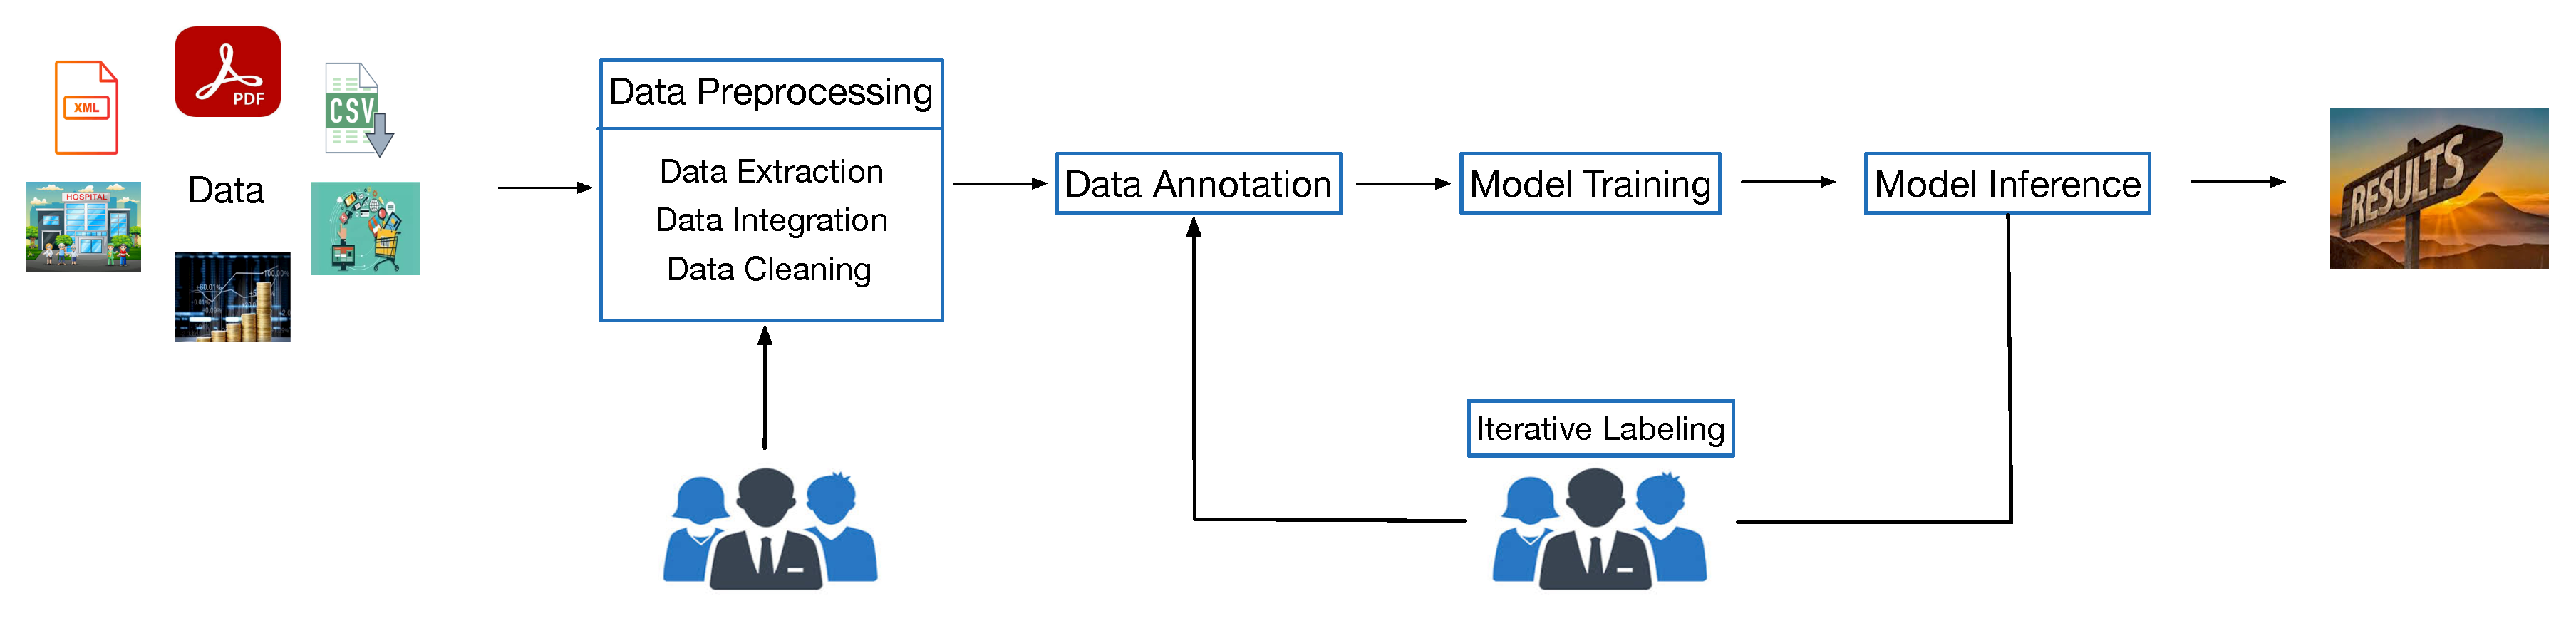
\includegraphics[width=0.65\textwidth]{
%NSFcore-2023/framework.pdf}
 %%\caption{Proposed Project}\label{project}
%\end{wrapfigure}



%We intend to propose complete, partial (either order or unordered), and various qualitative individual preference elicitation models.  An example of the first two would be having complete or only top-$k$ order of preferences over the candidates as inputs, whereas, an example of the last one  would be to bucketize candidates in different qualitative groups (recall the motivating example). For fairness, our effort would be to design group based fairness criteria designed over the protected attributes of the candidates that resemble group fairness criteria, such as, demographic parity, or statistical parity, studied in the context of classification~\cite{verma2018fairness}. To that end, we will adapt proportionate-fairness or p-fairness~\cite{pfair,chairman}  from resource allocation theory that ensures proportionate representation of every group based on a protected attribute in every position of the produced results, or its generalization~\cite{amer2009group} adapted from the social choice theory to promote affirmative action~\cite{fu2006theory} in the produced results.  
%Preference aggregation would be studied considering Kendall-Tau and Spearman's Footrule Distance functions~\cite{kemeny,diaconis1977spearman}, with the objective to minimize the sum of disagreement (Kemeny Optimization) or such, akin to existing {\em (fairness unaware) classical rank aggregation problem}~\cite{dwork2001rank,ailon2008aggregating, ailon2010aggregation}. Our goal would be to make these solutions fairness aware by investigating how to combine these two somewhat conflicting aspects in a systematic manner. For each of these proposed problem variants, we shall analyze the nature of the problem analytically and design scalable solutions with theoretical guarantees. Finally, we will perform both qualitative and quantitative study to develop actionable interventions by leveraging our proposed framework to promote fairness in two compelling applications: (i) Ranked Choice Voting (RCV)~\cite{rcv1,rcv2}, and (ii) Gender and diversity gap in the Oscars. We intend to fine-tune our proposed models based on these evaluations. 

\noindent {\bf Comparison with Existing Work.}
This contribution builds on our work recent works on fairness~\cite{islam2022satisfying, wei2022rank}, and prior works on preference aggregation~\cite{amer2009group, amer2015group, basu2015group}, studying robustness~\cite{roy2014exploiting}. We acknowledge that the existing popular group based fairness definition, such as, {\em statistical parity}~\cite{dwork2012fairness} is somewhat similar to one of our proposed fairness notion. However, the best adapted version of top-$k$ statistical parity studied in a recent paper~\cite{vldbrank} does not account for proportionate representation in every position of the top-$k$, limiting its applicability.  Studying computational challenges related to computing the margin of victory  has been a focus of recent research~\cite{stv1,stv2, stv3} in the context of electoral voting and related applications. But none of these existing works study the general version of the problem, which is, how to promote additional simple/complex constraints/criteria in the output, which is our primary focus. Other than these prior works, which are  much narrow in scope, we are unaware of any computational work that systematically studies different preference elicitation models, multiple output changing criteria, and preference aggregation combining these two.  

%Section~\ref{related} provides an in-depth comparison between our proposed work and existing work.  
%To the best of our knowledge, we are the first to investigate a generic framework that can minimally update original outcome of preference aggregation to satisfy complex constraints without any assumption on the relationship among the attributes.

%Using the aforementioned example, if $k=12$, existing work~\cite{vldbrank} only ensures p-fairness of the aggregated rank at position $12$, but not for the remaining positions (e.g., 1 to 11). {\em While p-fairness promotes stronger notion of fairness, and our proposed framework adapts to top-$k$ statistical parity, existing work does not adapt to our proposed optimization framework}.

%\smallskip \noindent {\bf Aim 1 - Fair Rank Aggregation.}
%We will begin our study in the context of ranking, which is a commonly used method to prioritize  desirable outcomes among a set of candidates and is an essential step in  many high impact applications. Here the members elicit a {\em complete preference order} over the candidates and the goal is to produce an aggregated ranked order over all candidates or produce top-$k$ results that minimize disagreements  among individual preferences. When fairness is studied, our goal would be to ensure fair representation of the candidates based on their one or more protected attributes (such as, gender, race, etc.) in the ranked order. 
%\smallskip \noindent {\bf Aim 2 - Fair Partial and Qualitative Preference Aggregation.}
%In this aim we shall consider scenarios where either qualitative preferences or partial rankings are elicited from the members. 
%We consider three such preferences: (1) top-$t$ ranking, where the input preference is a ranking of the top-$t$ items (candidates), (2) subset selection, where the input preference is an unordered subset of favorite elements, and (3) bucketing, where the input preference is a partition of the elements into three subsets: the ``yes'' set, ``ambivalent'' set, and the ``no'' set.  In our preliminary work, we consider the selection of council members or a committee of $k$ members from $n$ candidates considering the votes of $m$ judges (voters) ({\em ranked choice voting}~\cite{rank1} could be considered as a popular application of that).  The fairness criterion models affirmative action and includes a lower and upper bound on the number of elected candidates, for each value of the protected attributes(s). We intend to study the design choices of different preference elicitation models considering fairness, formalize the optimization problems and analyze them, and design principled solutions with guarantees.

%The mechanism we focus on to aggregate the top-$k$ rankings is {\em Ranked choice voting (RCV)}, and specifically RCV employing a single transferable vote (STV) system~\cite{rcvdesc}.
%We are going to follow the mechanism used in Cambridge MA to elect its city council. 

%\smallskip \noindent {\bf Aim 3 - Actionable Fair Preference Aggregation.}
%Although the proposed models and algorithms consider 
%fairness in its design, rather than an afterthought, the third aim will delve deeper into fairness considerations of compelling applications and develop actionable interventions. In particular, the third aim will provide a holistic large-scale study over two compelling applications and present actionable interventions to promote fairness. In the first application, we will study fairness in Ranked Choice Voting (RCV)\footnote{\small https://qz.com/1676718/the-pros-and-cons-of-ranked-choice-voting/} considering the data provided by the Cambridge, MA
%City Council Election 2019~\cite{RCV} to analytically answer important questions raised in recent research~\cite{rcv1,rcv2,rcv3, rcv4,rcv5}. 1. Does more choice lead to reduced racially polarized voting? 2. Does ranked choice voting enable minority representation?  Based on the analysis, {\em we will develop actionable interventions by leveraging our proposed framework to mitigate these risks}. We will perform both qualitative and quantitative analysis. For qualitative  analysis, we will recruit experienced workers from Amazon Mechanical Turk (the budget justification provided further details). A similar  study would be conducted to investigate the gender and diversity gap in the Academy of Motion Picture Arts and Sciences decisions by combining it with large scale Movielens~\cite{movielens} data and we will develop actionable recommendation to mitigate the gap. Further evaluation plan considering other datasets is described in Section~\ref{eval}.

%\section{Introduction}
\label{seC:intro}
% Interpretability and nutritional labels, generally

An essential ingredient of successful machine-assisted decision-making, particularly in high-stakes decisions, is interpretability --– allowing humans to understand, trust and, if necessary, contest, the computational process and its outcomes.   These decision-making processes are typically complex:  carried out in multiple steps, employing models with many hidden assumptions, and relying on datasets that are often repurposed --- used outside of the original context for which they were intended.\footnote{See Section 1.4 of Salganik's ``Bit by Bit''~\cite{salganik} for a discussion of data repurposing in the Digital Age, which he aptly describes as "mixing readymades with custommades.''}  In response, humans need to be able to determine the ``fitness for use'' of a given model or dataset, and to assess the methodology that was used to produce it.  

To address this need, we propose to develop interpretability and transparency tools based on the concept of a {\em nutritional label}, drawing an analogy to the food industry, where simple, standard labels convey information about the ingredients and production processes. Short of setting up a chemistry lab, the consumer would otherwise have no access to this information. Similarly, consumers of data products cannot be expected to reproduce the computational procedures just to understand fitness for their use.   Nutritional labels, in contrast, are designed to support specific decisions by the consumer rather than completeness of information.  A number of proposals for hand-designed nutritional labels for data, methods, or both have been suggested in the literature\cite{DBLP:journals/corr/abs-1803-09010,DBLP:journals/corr/abs-1805-03677,DBLP:conf/fat/MitchellWZBVHSR19}; we advocate deriving such labels automatically or semi-automatically as a side effect of the computational process itself, embodying the paradigm of {\em interpretability-by-design}. 

Interpretability means different things to different stakeholders, including individuals being affected by decisions, individuals making decisions with the help of machines, policy makers, regulators, auditors, vendors, data scientists who develop and deploy the systems, and members of the general public.  Designers of nutritional labels must therefore consider {\em what} they are explaining,  {\em to whom}, and {\em for what purpose}.  In the remainder of this section, we will briefly describe two regulatory frameworks that mandate interpretability of data collection and processing to members of the general public, auditors, and regulators,  where nutritional labels offer a compelling solution (Section~\ref{sec:intro:reg}).  We then discuss interpretability requirements in data sharing, particularly when data is altered to protect privacy or mitigate bias (Section~\ref{sec:intro:synth}).

\subsection{Regulatory Requirements for Interpretability}
\label{sec:intro:reg}

The European Union recently enacted a sweeping regulatory framework known as the General Data Protection Regulation, or the GDPR~\cite{gdpr}.  The regulation was adopted in April 2016, and became enforceable about two years later, on May 25, 2018.  The GDPR aims to protect the rights and freedoms of natural persons with regard to how their personal data is processed, moved, and exchanged (Article 1).  The GDPR is broad in scope, and applies to ``the processing of personal data wholly or partly by automated means'' (Article 2), both in the private sector and in the public sector.  Personal data is broadly construed, and refers to any information relating to an identified or identifiable natural person, called the {\em data subject} (Article 4).  

According to Article 4, lawful processing of data is predicated on the data subject's {\em informed consent}, stating whether their personal data can be used, and for what purpose (Articles 6, 7).
Further,  data subjects have {\em the right to be informed} about the collection and use of their data.~\footnote{\url{https://gdpr-info.eu/issues/right-to-be-informed/}}
Providing insight to data subjects about the collection and use of their data requires technical methods  that support interpretability.  

Regulatory frameworks that mandate interpretability are also starting to emerge in the US.  New York City was the first US municipality to pass a law (Local Law 49 of 2018)~\cite{Vacca}, requiring that a task force be put in place to survey the current use of ``automated decision systems'' (ADS) in city agencies. ADS are defined as ``computerized implementations of algorithms, including those derived from machine learning or other data processing or artificial intelligence techniques, which are used to make or assist in making decisions.''   The task force is developing recommendations for enacting algorithmic transparency by the agencies, and will propose procedures for: (i) requesting and receiving an explanation of an algorithmic decision affecting an individual (Section 3 (b) of Local Law 49); (ii) interrogating ADS for bias and discrimination against members of legally protected groups, and addressing instances in which a person is harmed based on membership in such groups (Sections 3 (c) and (d)); (iii) and assessing how ADS function and are used, and archiving the systems together with the data they use (Sections 3 (e) and (f)).

Other government entities in the US are following suit.  Vermont is convening an Artificial Intelligence Task Force to ``... make recommendations on the responsible growth of Vermont’s emerging technology markets, the use of artificial intelligence in State government, and State regulation of the artificial intelligence field.''~\cite{Vermont}.  Idaho’s legislature has passed a law that eliminates trade secret protections for algorithmic systems used in criminal justice~\cite{Idaho}.  In early April 2019, Senators Booker and Wyden introduced the Algorithmic Accountability Act of 2019 to the US Congress~\cite{BookerWydenClarke}. The Act, if passed, would use ``automated decision systems impact assessment'' to address and remedy harms caused by algorithmic systems to federally protected classes of people. The act empowers the Federal Trade Commission to issue regulations requiring larger companies to conduct impact assessments of their algorithmic systems.

The use of nutritional labels in response to these and similar regulatory requirements can benefit a variety of stakeholders.  The designer of a data-driven algorithmic method may use them to validate assumptions, check legal compliance, and tune parameters.  Government agencies may exchange labels to coordinate service delivery, for example when working to address the opioid epidemic, where  at least three sectors must coordinate: health care, criminal justice, and emergency housing, implying a global optimization problem to assign resources to patients effectively, fairly and transparently. The general public may review labels to hold agencies accountable to their commitment to equitable resource distribution. 


\subsection{Interpretability with Semi-synthetic Data}
\label{sec:intro:synth}

%Datasets are now increasingly used to train models to make decisions once made by humans.  In these automated systems, biases in the data are propagated and amplified with no human in the loop.  The bias, and the effect of the bias on the quality of decisions made, is not easily detectable due to the relative opacity of the system.  

A central issue in machine-assisted decision-making is its reliance on historical data, which often embeds results of historical discrimination, also known as {\em structural bias}.   As we have seen time and time again, models trained on data will appear to work well, but will silently and dangerously reinforce discrimination~\cite{propublicaJ,amazon_hiring,amazon_delivery}.  Worse yet, these models will legitimize the bias --- ``the computer said so.''  Nutritional labels for data and models are designed specifically to mitigate the harms implied by these scenarios, in contrast to the more general concept of ``data about data.''

Good datasets drive research: they inform new methods, focus attention on important problems, promote a culture of reproducibility, and facilitate communication across discipline boundaries.  But research-ready datasets are scarce due to the high potential for misuse. Researchers, analysts, and practitioners therefore too often find themselves compelled to use the data they have on hand rather than the data they would (or should) like to use.  For example, aggregate usage patterns of ride hailing services may overestimate demand in early-adopter (\ie wealthy) neighborhoods, creating a feedback loop that reduces service in poorer neighborhoods, which in turn reduces usage.  In this example, and in many others, there is a need to alter the input dataset to achieve specific properties in the output, while preserving all other relevant properties.  We refer to such altered datasets as \textit{semi-synthetic}.

Recent examples of methods that produce semi-synthetic data include database repair for causal fairness~\cite{DBLP:conf/sigmod/SalimiRHS19}, database augmentation for coverage enhancement~\cite{DBLP:conf/icde/AsudehJJ19}, and privacy-preserving and bias-correcting data release~\cite{DBLP:conf/ssdbm/PingSH17,DBLP:conf/vldb/RodriguezSPSH18}. A semi-synthetic datasets may be altered in different ways.  Noise may be added to it to protect privacy, or statistical bias may be removed or deliberately introduced.  When a dataset of this kind is released, its composition and the process by which it was derived must be made interpretable to a data scientist, helping determine fitness for use.  For example, datasets repaired for racial bias are unsuitable for studying discrimination mitigation methods, while datasets with bias deliberately introduced are less appropriate for research unrelated to fairness.   This gives another compelling use case for nutritional labels.

%To make our discussion more concrete, let us consider data scientists who must identify datasets appropriate for their task.  This is particularly important when semi-synthetic datasets are being released, to which noise is added to protect privacy, or statistical bias is removed or deliberately introduced.  For example, datasets repaired for racial bias are unsuitable for studying discrimination mitigation methods, while datasets with bias deliberately introduced are less appropriate for research unrelated to fairness.  



%\input{IEEE-data-engineering-IC1/preliminary}
\vspace{-0.2in}
\section{Formalism}\label{preliminary}
\vspace{-0.1in}
%The proposed work aims at developing an optimization guided computational framework that modifies an output obtained from a preference aggregation method applied on a preference elicitation model to produce a modified output that satisfies given criteria. The proposed work aims at developing this framework for a suite of preference elicitation models and preference aggregation methods.
%that satisfies with criteria that guides the need to change the original output minimally while producing a complete or top-$k$ (ordered or unordered) result aggregating individual preferences.

There are $4$ types of inputs that our proposed framework takes: (a)~a set $N$ of $n$ items, where each item has a set $\mathcal{A}$ of discrete attributes.  Each attribute $a\in \mathcal{A}$ has $\ell_a$ different values. (b)~a set of $m$ users, where the $i$-th user $u(i)$ provides her preference as $\sigma_i$. The users' preferences could be rank based, partial or full order, or non rank based. (c)~a distance function $\mathcal{F}$ (defined formally below) that measure the ``distance'' between a set of $m$ input preferences  $\sigma_1, \sigma_2,\ldots, \sigma_m$ and an output $\sigma$ with the required output form. The exact distance function depends on the underlying preference elicitation model and the required output form which may be either a complete ranking of the items or a subset of $k$ items, either ranked or not. (d)~a set $\mathcal{C}$ of output criteria/constraints. Some variants of our problem also include as input a budgetary constraint $B$.

%The proposed work aims at developing an optimization guided computational framework that suitably combines a suite of preference elicitation models with criteria that guides the need to change the original output minimally while producing a complete or top-$k$ (ordered or unordered) result aggregating individual preferences. %Next, we present some definitions that will be used throughout the proposal.  

\begin{definition}\label{def4}
\vspace{-0.1in}
{\bf Distance function $\mathcal{F}$.} Given $m$ input preferences  $\sigma_1, \sigma_2,\ldots, \sigma_m$ and an output $\sigma$ with the required output form, the function $\mathcal{F}(\sigma, \sigma_1, \sigma_2,\ldots, \sigma_m)$ is the distance of $\sigma$ from the input preferences  $\sigma_1, \sigma_2,\ldots, \sigma_m$.
In some cases the function $\mathcal{F}(\cdot)$ is an aggregation of a distance function between a single input preference and the output. Examples for such an aggregation are the sum of the pairwise distances and the maximum distance to any of the input preferences. In other cases $\mathcal{F}(\cdot)$ measures the minimum modification of the input preferences that would result in the preference aggregation method outputting the output $\sigma$. 
%$\mathcal{F}(\sigma, [\sigma_1, \sigma_2,\ldots, \sigma_m])$
\end{definition}

\vspace{-0.1in}
\begin{definition}\label{def1}
\vspace{-0.1in}
{\bf Output criteria/constraints.}  For an attribute $a\in \mathcal{A}$,  let $c(p_a)$ denote the cardinality constraints of items with value $p_a$ ($p_a$ is one of the $\ell_a$ possible values of attribute $a$). Given to the framework is a set $C$ of such cardinality constraints for each attribute value $p_a$, for every $a \in A$, $A \subset \mathcal{A}$. There are two explicit cases that we consider.
\begin{itemize}
    \item {\bf The output $\sigma$ is ordered and consists of $k\le n$ items.} 
    In this case the cardinality constraints are defined for every $\kappa \in [1..k]$ items, and for every  such $\kappa \in [1..k]$, the $\kappa$ top ranked items of output $\sigma$ have to satisfy these cardinality constraints.  
    %the $k$ top ranked items satisfy all cardinality constraints defined over $v$, i.e., it satisfies $c(p^v_{a_1}) \text{ AND } c(p^v_{a_2}) \text{ AND } \ldots \text{ AND } c(p^v_{a_A})$.  
     \item {\bf The output $\sigma$ is an unordered set of $k$ items.} In this case the cardinality constraints are defined for $k$ items and the items in the output set $\sigma$ have to satisfy these cardinality constraints. 
     \\ %$c(p_{a_1}) \text{ AND } c(p_{a_2}) \text{ AND }  \ldots \text{ AND } c(p_{a_A})$.  
\end{itemize}  
\end{definition}
\vspace{-0.1in}
\begin{definition}\label{def3}
\vspace{-0.1in}
{\bf A budgetary constraint.} A budgetary constraint $B$ is an upper bound on the distance of the output from the input preferences. 
%For a given distance function $\mathcal{F}(\cdot)$, 
The budgetary constraint implies that $\mathcal{F}(\sigma,\sigma_1,\sigma_2,\ldots,\sigma_m)\leq B$.  
\end{definition}

\vspace{-0.1in}
\begin{definition}\label{def2}
{\bf Preference Aggregation Considering Constraints.} 
We intend to study different types of problem definitions that require different algorithmic treatments.
Given either complete or partial preferences $\sigma_1,\sigma_2,\ldots,\sigma_m$ over the items in $N$, a preference aggregation method, a distance function $\mathcal{F}(\cdot)$, and a set of output criteria $\mathcal{C}$.
\vspace{-0.1in}
\begin{itemize}
    \item {\bf (Constrained optimization).} Produce an output $\sigma$ with the required form that minimizes $\mathcal{F}(\sigma,\sigma_1,\sigma_2,\ldots,\sigma_m)$ and satisfies $\mathcal{C}$.
    \vspace{-0.1in}
    \item {\bf (Optimization under budgetary constraints).} Produce an output $\sigma$ with the required form that optimizes $\mathcal{C}$,  while satisfying $\mathcal{F}(\sigma,\sigma_1,\sigma_2,\ldots,\sigma_m) \leq B$. (The objective function for optimizing $\mathcal{C}$ varies.)
    \vspace{-0.1in}
    \item {\bf (Bi-criteria optimization).} Given parameters $\alpha$ and $\beta$ produce an output $\sigma$ with the required form that satisfies both $\mathcal{F}(\sigma,\sigma_1,\ldots,\sigma_m) \le \alpha$ and $\mathcal{G}(\mathcal{C}) \le \beta$, where $\mathcal{G}$ is the objective function for optimizing $\mathcal{C}$.
\end{itemize}
\end{definition}
%The individual research aims will describe the various forms of preference elicitation from users and the details of the preference aggregation methods. We first delineate the need to change original output and the challenges that arise from there.
\vspace{-0.1in}
\subsection{Specifying Output Criteria}
We discuss orthogonal reasons where the original outputs coming out of the preference aggregation methods need to be ``massaged'' further. What unifies them is that these criteria are defined over one or more attributes of the items. Depending on how many attributes are involved in the definition and their relationship thereof gives rise to additional challenges.


%\vspace{-0.1in}
%\subsection{Important Concepts and Definitions}\label{pre}
%\vspace{-0.1in}
%\noindent \textbf{Database.} contains $n$ items or candidates. These two terms will be used interchangeably. The set of items will be denoted $V$, individual items will be denoted by $u$ and $v$. \\
%\noindent {\em \bf Individual preference Elicitation:} We consider the following individual preference elicitation models. \\
%\noindent (1) Complete preference: Each of the $4$ members (Judges) may provide a {\em complete order of preference} over the $12$ candidates (Refer to Table~\ref{tab:example_original_rank}). \\
%\noindent (2) Partial preference: 
%(2.1) Ordered. Member 1 (as well as other members) may provide a partial order over the first $5$ candidates and does not specify anything for the rest.\\
%(2.2) Unordered. Member 1 (as well as other members) may also specify that she likes the first $5$ candidates without specifying any order among them.\\
%\noindent (3) Qualitative Preference: Contrarily, Member 1 (as well as other members) may provide {\em qualitative preferences}: Molly and Amy are preferred, Abigail, Kim, Lee are acceptable, the remaining ones must not be considered. These are considered to be the inputs to the framework. Please note that 2.2 is a simplified variant of this last preference elicitation model.

%\noindent \textbf{Multiple Preferences.} The input consists $m$ different preference elicitation (based on the individual models described above). Using the motivating example, $m=4$.

\subsubsection{Fair Preference Aggregation}
We will study fairness in the context of group based protected attributes of the candidates. Output criteria/constraints for fairness (refer to Definition~\ref{def1}) are expressed over one or more {\em protected attributes}. Their protected attributes could be expressed over gender, ethnicity, race, or the state the candidates are living in. 

Formally speaking, each item/candidate $v\in N$ has one or more  {\em protected attributes}. When $\ell_a=2$, it is a binary protected attribute; when $\ell_a \geq 2$ it is a multi-valued protected attribute. As an example, race is (usually) a multi-valued protected attribute, and gender is sometimes a binary protected attribute.

%\begin{itemize}
%\item  {\bf p-fairness.} 
\smallskip \noindent \textbf{p-fairness.}
p-fairness has been studied in the context of resource allocation satisfying temporal fairness or proportionate progress~\cite{chairman, pfair}. It was introduced in the classical  {\em Chairman Assignment Problem}~\cite{baayen1964existence, chairman} that studies how to select a chairman of an union every year from a set of  $n$ states such that  that at any time the accumulated number of chairmen from each state is proportional to its weight. 

In the context of ranking, suppose that each of the $n$ ranked items has a {\em protected attribute} $a(\cdot)$ that can take any of $\ell_a$ different values. For $p_a\in [1..\ell_a]$, let $c'(p_a)$ denote the fraction of items with protected attribute value $p_a$, that is, $c'(p_a) = \frac 1n \sum_{i=1}^n \bbone_{a(i)=p_a}$. The goal is to ensure that $c'(p_a)$ fraction (rounded either up or down) of every top $\kappa$ items have protected attribute value $p_a$.
\iffalse
\vspace{-0.1in}
\item {\bf Generalization of p-fairness to promote affirmative action.} Instead of requiring $c'(p_a)$ fraction of every top $\kappa$ items to have protected attribute value $p_a$, we may want that certain values of the protected attribute get higher representation among the elements at the top, more than their overall proportion. Let $P$ be a non-negative doubly stochastic $n \cdot \ell_a$ matrix. The goal is to ensure that $P(\kappa,p_a)$ fractions (rounded either up or down) of the top $\kappa$ items to have value $p_a$, for every $\kappa \in [1..n]$ and $p_a\in [1..\ell_a]$ (if it is feasible).
It is not difficult to note that such a generalized notion can capture affirmative action.
%\end{itemize}
\fi


\subsubsection{Robust Preference Aggregation}
Output criteria/constraints for robustness on the other hand investigates the flip questions: Given either complete or partial preferences $\sigma_1,\sigma_2,\ldots,\sigma_m$ over $n$ items, let $\sigma$ be the output obtained by the preference aggregation method. Given a budget $B$, how to  make $B$ or less changes in the original preferences, such that the outcome is different from $\sigma$? This question is  related to finding the {\em margin} in electoral systems and quantifies how manipulable the underlying aggregation method is. We study this problem under different manipulation models -- addition only, deletion only, or substitution (addition + deletion).

\iffalse
\subsection{Challenges in Handling  Complex Output  Criteria}
In general, the output requirements/constraints are defined over a set $R$ of attributes. When $|R|=1$, as an example, the output requirement is defined on a single attribute (such as race). In a recent work, we demonstrated that for an aggregation method that models plurality voting, the problem of preference aggregation while satisfying output criteria defined by a single attribute is computationally easy. 
However, the nature of the problem changes when two or more attributes are involved in the output criteria. In Section~\ref{aim1} we discuss this more complicated case and refer to our recent work in which we showed evidence that in some cases it is computationally difficult even to find any output with the required form. 
\fi
%When there are two or more different attributes involved in outlining output criteria/constraints (such as certain representation from race and certain representation from gender), the PIs have proved in a recent work~\cite{islam2022satisfying} that the decision version of the preference aggregation problem under output constraint becomes (weakly) NP-hard by reducing the well known NP-hard Partition problem to our problem~\cite{garey1979computers}. We note that the existing practice of converting multiple attributes to a single multi-valued protected attribute by computing joint distribution over the attributes assumes independence among the attributes. When Independence among the attributes does not hold, this simplification leads to a heuristic process.  The PIs have also demonstrated that for three (or more) attributes (e.g., constraints defined over race, and gender, and ethnicity), even the question whether there exists a set of top-$k$ that satisfies the complex constraint is strongly NP-Hard where the reduction is fro 3 Dimensional Matching. On the positive side for the case of two  attributes, the PIs have designed an efficient algorithm a preference aggregation algorithm while satisfying fairness constraints defined over $2$ attributes and has designed a 2 approximation factor and runs in $O(n^2\ell \log m)$ time, by casting this problem as a min cost flow problem, where $\ell$ is the total number of possible attribute values. We intend to study these aspects in the proposal - as it turns out to be an intellectually demanding and independent  facet of the computational problem, irrespective of the specific reasons to change the output.


%\input{IEEE-data-engineering-IC1/aim1}
\vspace{-0.2in}
\section{Single Round Rank based Preference Aggregation}\label{aim1}
\vspace{-0.1in}
We outline two separate lines of algorithmic problems: (1) incorporating output criteria (e.g., p-fairness) in single round rank-based preference aggregation methods, and (2) satisfying complex constraints in single round rank-based preference aggregation methods.
\vspace{-0.1in}
\subsection{Incorporating output criteria in rank aggregation} 
\vspace{-0.1in}
The input to the classical {\em rank aggregation} problem consists of $m$ complete order of preferences over the $n$ items/candidates. Traditionally, producing the final ranking involves aggregating potentially conflicting preferences from multiple individuals, and is known as the rank aggregation problem~\cite{dwork2001rank,van2007deterministic, ailon2008aggregating}. Our goal is to  minimally change the aggregated output to enable fairness.
%p-fairness has been studied in the theory community to enable resource allocation satisfying temporal fairness or proportionate progress.
We will study p-fairness~\cite{chairman, pfair} that ensures proportionate representation of every group based on a protected attribute in every position of the aggregated ranked order.  The classical problem in this context is known as the {\em Chairman Assignment Problem}~\cite{baayen1964existence, chairman} which studies how to select a chairman of a union every year from a set of  $r$ states such that  that at any time the accumulated number of chairmen from each state is proportional to its weight. p-fairness generalizes other notions of fairness~\cite{islam2023equitable} that were considered in prior work, including the existing popular group based fairness definition {\em statistical parity}~\cite{dwork2012fairness}. 
%We start with some definitions and then describe both our preliminary research and the open problems we plan to investigate further.
\vspace{-0.1in}
\subsubsection{Research Directions}
\vspace{-0.1in}
%\noindent \textbf{Rank and Multiple Ranking.}  
Consider rankings of the items in a set $V$. Each such ranking can be viewed as a permutation. We will use the terms ranking and permutation interchangeably. 

\noindent \textbf{Kendall-Tau and Kemeny distances.}
	Given two rankings $\sigma,\eta: V \rightarrow [1..n]$, the
	Kendall-Tau distance between the two rankings is the sum of pairwise disagreements between $\sigma$ and $\eta$ (bubble-sort distance)
	\[
	\cK (\sigma,\eta) = \sum_{\{u,v\}\subseteq V} \bbone_{(\sigma(v)-\sigma(u))(\eta(v)-\eta(u))<0}.
	\]
	
	For a set of rankings
	$\{\eta_1,\eta_2,\ldots,\eta_m\}$ the {\em Kemeny distance} of the ranking
	$\sigma$ to this set as
	\[
	\kappa(\sigma,\eta_1,\eta_2,\ldots,\eta_m)= \sum_{i=1}^m \cK (\sigma,\eta_i).
	\]

 \noindent \textbf{Spearman's footrule distance.}
    Given two rankings $\sigma,\eta: V \rightarrow [1..n]$, the 	Spearman's footrule distance between the two rankings is the sum of the absolute values
  ($\ell_1$ distance) of the differences between rankings $\sigma$ and $\eta$.
	\[
	\cS (\sigma,\eta) = \sum_{u\in V} |(\sigma(u)-\eta(u)|
	\]
 
	For a set of rankings
	$\{\eta_1,\eta_2,\ldots,\eta_m\}$ the {\em Spearman's footrule distance} of the ranking
	$\sigma$ to this set is the sum of the pairwise distances.

    \noindent \textbf{Rank aggregation.} The aggregated ranking of a set of $m$ rankings $\{\rho_1,\rho_2,\ldots,\rho_m\}$ for a given distance function is a ranking that minimizes  the distance to this set.
    
    \noindent \textbf{p-fairness for a ranking.}
    For a permutation $\sigma, k\in [1..n], p\in [1..\ell]$, let $P(\sigma,k,p)$ denote
    the number of elements with protected attribute value $p$ among the $k$ top ranked elements
    in $\sigma$. A ranking $\sigma$ is {\em proportionate fair} or {\em p-fair} if
    \[
    \forall k\in [1..n]\, \forall p\in [1..\ell]:\  P(\sigma,k,p)\in \{\floor{f(p)\cdot k},\ceil{f(p)\cdot k}\}.
    \]

 
%We note that the best adapted version of top-$k$ statistical parity studied in a recent paper~\cite{vldbrank} does not account for proportionate representation in every position in the top-$k$ positions, but just to a small number of positions, thus limiting its applicability.
%As a matter of fact it can be shown that the algorithm Fair-ILP presented in~\cite{vldbrank} for the special case of a binary protected attribute in which the frequency of both values is the same may produce a very skewed output. This is because the algorithm Fair-ILP just considers the {\em total number of times} items with one value of protected attribute are ranked above items with the other value. p-fairness is  stronger because it ensures statistical parity for every position in the ranked order and considers, for every $k$, the number of times items in the top-$k$ with one value of protected attribute are ranked above items with the other value. This makes this notion of fairness significantly harder to implement and the existing solutions do not trivially adapt.


We formalized two optimization problems, individual p-fairness or {\bf IPF} and the rank aggregation problem subject to proportionate fairness ({\bf RAPF})  considering binary ($\ell=2$) and multi-valued ($\ell > 2$) protected attributes. These problems and associated algorithmic results could be found in~\cite{wei2022rank}.


\vspace{-0.1in}
\subsubsection{Open Problems}
\vspace{-0.1in}
We plan to investigate the following open problems.

\smallskip \noindent{\bf p-fairest aggregate ranking (PFAR).} 
The PFAR problem is defined as follows. Given a set of $m$ rankings %$\{\rho_1,\rho_2,\ldots,\rho_m\}$ 
choose the ``p-fairest'' ranking among all rankings that minimize the Kemeny distance to this set. 
We need to define ``p-fairest'' ranking or a distance measure to a p-fair ranking.
We propose the following distance measure (using the notations defined above).
For an integer $d \ge 0$, a ranking $\sigma$ is at distance $d$ from a {\em p-fair} ranking if
\[
\forall k\in [1..n]\, \forall p\in [1..\ell]:\  P(\sigma,k,p)\in \{\floor{f(p)\cdot k}-d,\ceil{f(p)\cdot k}+d\}.
\]

\iffalse
Another way to view the distance to a p-fair ranking is by considering the classical {\em p-processor cup game} defined by Liu~\cite{liu1969} that considered the notion of p-fairness in multi processor scheduling. The p-processor cup game (adapted to our case) is a multi-round game with two players, an {\em emptier} and a {\em filler}, that takes place on $\ell$ cups, each filled initially with a fixed amount of water, called {\em buffer}. At the beginning of each round,
the filler adds a total of 1 gallon of water to the cups. The distribution of this 1 gallon to the cups is determined by the filler.
The emptier then selects a single cup (that must have at least 1 gallon of water)
and removes 1 gallon from this cup. The emptier’s goal is to minimize the size of the buffer and the {\em backlog} which is the amount of water (on top of the initial amount) in the fullest cup.

It is easy to see the analogy to p-fairness. Consider a p-fair ranking of $n$ elements each with a protected attribute with $\ell$ possible values. Each cup represents a possible value of the protected attribute. The corresponding game has $n$ rounds. In each round $k\in [1..n]$ the filler
adds $f(p)$ gallons of water to cup $p$, for $p\in [1..\ell]$, and the emptier removes 1 gallon of water from the cup corresponding to the value of the protected attribute of the element ranked $k$.
The existence of a p-fair ranking implies that the emptier can always guarantee that the size of the buffer and the backlog is no more than 1 gallon.
For a ranking that is at distance $d$ from a p-fair ranking, the emptier can guarantee that the size of the buffer and the backlog is no more than $1+d$ gallons.
\fi

We observe that PFAR is also NP-Hard as directly follows from the fact that unconstrained rank aggregation is NP-hard when 
$m\ge 4$~\cite{ailon2008aggregating}. For some fixed $\alpha > 1$, We would like to find an algorithm that finds the p-fairest ranking among all rankings whose Kemeny distance from the set of input rankings is at most $\alpha$ times the minimum such distance. 
%Reasonable values of $\alpha$ to consider are 
%$\frac 85$ and $\frac 43$ since there are efficient $\frac 85$ and $\frac 43$ approximation algorithm for the rank aggregation problem~\cite{ailon2008aggregating}.

\smallskip \noindent {\bf Bi-criteria p-fair rank aggregation (BPFRA).} 
The most general problem that we plan to consider in this context is the bi-criteria optimization problem, that is, for a given pair $(\alpha>1 ,\beta>1)$ and a set of $m$ rankings %$\{\rho_1,\rho_2,\ldots,\rho_m\}$
find a ranking whose Kemeny distance to the set of rankings is at most $\alpha$ times the Kemeny distance of the aggregated rank from the set and its distance from a p-fair ranking is at most $\beta$, if such a ranking exists.

\smallskip \noindent{\bf p-fair rank aggregation with affirmative action.} 
We plan to consider a variant of p-fair rank aggregation that involves ``affirmative action''. This will be modeled by varying the proportion of the values of the protected attribute in the p-fair aggregated rank. For example, consider a binary protected attribute with values A and B each needs to appear the same number of times. Suppose that our goal is to promote the items with attribute value A. In this case we can vary the proportion of A making it higher in the top ranked elements and lower in the lower ranked elements so that overall items with attribute value A will appear the same number of times as items with attribute value B.

\smallskip \noindent{\bf The complexity of individual p-fair ranking (IPF).}  We plan to further investigate the IPF problem for multi valued protected attributes as it is open whether it can be solved accurately in polynomial time. We conjecture that this problem is NP-Hard. %and plan to look for a suitable reduction to prove this conjecture. 
We also plan to look for improved approximation algorithms for this problem.
%We note that the algorithm DetConstSort given in~\cite{kddrank} does not produce closest ranking to a given input ranking.

\smallskip \noindent {\bf Better approximation of rank aggregation subject to p-fairness (RAPF).}
We plan to develop more sophisticated RAPF algorithms with better approximation ratios,  %One approach for designing such algorithms is to apply the pivoting technique presented in~\cite{ailon2008aggregating} for rank aggregation. We also plan 
and to improve the computational aspects of the RAPF problem. This problem can be formulated as an Integer Programming (IP) problem. %and thus the RAPF problem of reasonable size can be solved in practice using an IP solver like Gurobi or CPLEX.
We plan to consider various IP formulations as well as various rounding techniques to accelerate the computation.

\smallskip \noindent{\bf Robust rank aggregation.} It is known that rank aggregation under Kemeny distance is NP-hard. We will explore other aggregation methods, such as Spearman's footrule and Borda, and study how manipulable these rank aggregation methods are -- that is, if only $x\%$ of the preferences are allowed to be changed, how easy it is to change the outcome.
\vspace{-0.1in}
\subsection{Complex Constraints} 
\vspace{-0.1in}
Our goal is to optimize preference substitution to satisfy complex top-$k$ fairness constraints, where the fairness requirement is defined over a set $R$ of protected attributes. One of the objectives we will consider is {\em minimizing the number of single ballot (ranking) substitutions that guarantee fairness in the top-$k$ results.} 
%In voting theory~\cite{cary2011estimating}, the concept of margin of victory (MOV) is designed to measure electoral competitiveness of the candidates. 
In a preliminary work we defined the problem of finding the smallest number of single ballot substitutions to promote a set of $k$ candidates that satisfy fairness requirements defined over a set $R$ of protected attributes to the top-$k$. 
\vspace{-0.1in}
\subsubsection{Research Directions}
\vspace{-0.1in}
We assume that there are $\ell$ protected attributes , denoted $A_1,\dots, A_\ell$. For $i\in [1..\ell]$, attribute $A_i$ has $\ell_i$ possible values, denoted $A[i,j]$, for $j\in [1..\ell_i]$. Each candidate is associated with a specific value from each attribute.
In addition, we are given target quantities $a[i,j]$, for $i\in [1..\ell]$, and  $j\in [1..\ell_i]$, with property that all row marginals sum to $k$. Namely, for every $i\in [1..\ell]$, $\sum_{j=1}^{\ell_i} a[i,j] = k$. A fair outcome should satisfy the fairness  condition that for $i\in [1..\ell]$, and  $j\in [1..\ell_i]$, exactly $a[i,j]$ candidates whose $A_i$ attribute value is $A[i,j]$ are elected. 

\noindent We note that one way to approach this problem is by converting the multiple protected attributes to a single multi-valued protected attribute by computing joint distribution over the attributes assuming their independence. For example, instead of considering two binary valued attributes $A_1$ and $A_2$ we consider a single attribute with 4 possible values and the requirement that the value $i*j$ should appear $a[1,i]\cdot a[2,j]/k$ times, for $i,j\in \{1,2\}$. The shortcomings of this approach are two-fold: First, this approach may yield that the problem is infeasible while there is still a solution without assuming independence. A solution that assumes independence may be inferior (require more substitutions) than a solution that does not assume independence.

\noindent In~\cite{islam2022satisfying}, we showed that the problem of finding the smallest number of single ballot substitutions (original preference) to promote a set of $k$ candidates that satisfy proportionate representation over a single protected attribute is computationally easy for any domain size of the protected attribute. On the other hand the same problem becomes computationally hard if we increase the number of protected attributes. When there are two different protected attributes involved in outlining the fairness requirement, we proved that the decision version of that problem is (weakly) NP-hard, %by reducing the well known NP-hard Partition problem to our problem~\cite{garey1979computers}. 
For three (or more) protected attribute, even the question whether there exists a set of top-$k$ that satisfies the complex fairness constraint is strongly NP-Hard by a reduction from 3 Dimensional Matching. On the positive side for the case of two protected attributes we designed an efficient algorithm that obtains a 2 approximation factor and runs in $O(n^2\ell \log m)$ time, 
%by casting this problem as a min cost flow problem, 
where $\ell$ is the number of possible attribute values. We also designed an exact algorithm with running time $n^c$, where $c$ is the size of the Cartesian product of all the attribute domains.

\vspace{-0.1in}
\subsubsection{Open Problems}
\vspace{-0.1in}
There propose two possible ways to extend these problems.

\smallskip \noindent {\bf Improved approximation ratio in the case of 2 protected attributes.} 
Since  the problem of minimizing the number of single ballot substitutions in the case of 2 attributes is currently proven to be weakly NP-Hard, it may admit a PTAS (Polynomial Time Approximation Scheme). We plan to investigate the existence of a better approximation algorithm. Alternatively, we will try to improve the hardness result and show that this problem is strongly NP-Hard or Max-SNP Complete. 

\smallskip \noindent {\bf Relaxed solutions in the case of 3 or more protected attributes.} 
Clearly, the hardness result of even checking the existence of a solution in case of 3 or more attributes precludes the existence of any approximation algorithm for this case. We plan to design an algorithm that will generate a relaxed set of items/candidates. The relaxation may be in two dimensions: (i) the generated set will be a top-$k$ set of candidates but the fairness requirements will not be fully satisfied for all protected attributes. (ii) the generated set will have size larger than $k$ but it will satisfy the (lower bounds of the) fairness constraints for top $k$. Clearly, the larger the generated set is the easier the problem. We will find the smallest such extended set that guarantees the fairness  constraints imposed by all protected attributes.


%\input{IEEE-data-engineering-IC1/Aim2}
\vspace{-0.1in}
\section{Multi Round Rank based Preference Aggregation}\label{aim2}
\vspace{-0.1in}
We study algorithmic challenges to satisfy  output constraints in multi-round rank based preference aggregation methods, popularly known as ranked choice voting or (RCV)~\cite{irv1}. 
\vspace{-0.1in}
\subsection{Research Directions}
\vspace{-0.1in}
We start by describing the STV (single transferable vote) method~\cite{stv-irv, stv1} that generalizes the IRV method, and selects a set of $k$ items/candidates as the winners. STV is gaining popularity as an electoral system. It is used to elect candidates to the Australian Senate, in all elections in Malta, in most elections in the Republic of Ireland, and in Cambridge, MA. There are also plans to use STV in other USA localities. As mentioned in Section~\ref{preliminary} this method of preference aggregation is also applicable in other settings.

The input to an STV preference aggregation method consists of $m$ either complete or partial rankings of the items/candidates. Suppose that the total number of items/candidates is $n$ out of which $k$ items need to be elected. The preference aggregation process requires a predefined {\em quota}. In most cases this quota is Droop quota~\cite{droop} defined as $\floor{\frac{n}{k+1}}+1$. The aggregation is done in rounds. In each round every item/candidate is associated a {\em tally}. Initially, the tally of every item is the number of rankings in which it is ranked highest. A round starts by considering the items whose tally is at least the quota. These items are elected in non-increasing order of their tally, as long as $k$ items/candidates have not been elected (which always holds for Droop quota). When an item is elected their ``surplus'' (the number by which their tally exceeds the quota) is distributed to the next preferred item in their ranking (that has not been eliminated yet). The exact way this ``surplus'' is allocated varies. In a most cases, this allocation is done either fractionally or by a random selection of the surplus rankings out of all the  rankings in which the elected item is top ranked. This is repeated as long as there are items whose tally is at least the quota (and $k$ items/candidates have not been elected). 
Then, if less than $k$ items/candidates are elected, the item/candidate with the smallest tally is eliminated from all the rankings, and the tallies are updated based on the new rankings. If the number of items/candidates remaining (not elected and not yet eliminated) equals the
number of items/candidates left to be elected, these candidates are elected and the STV process terminates, otherwise the process repeats.

There is evidence that IRV and thus also STV preference aggregation methods are computationally hard to manipulate. It is NP-Hard to decide whether an IRV method can be manipulated even by adding one complete ranking~\cite{stv2}. On the positive side, \cite{blom2016,blom2019,magrino2011} suggested branch and bound algorithms that use Integer Programming to compute the Margin of Victory (MOV) in IRV. 

\iffalse
In our preliminary work, 
we considered the selection of $k$ council members out of $n$ {\em candidates} by $m$ voters or {\em members} with no ranking among the $k$ selected candidates. The fairness criterion %for this scenario is quite straightforward: 
is to maintain the proportion of each value of the protected attributes(s) within the selected candidates as in the whole set of candidates, or its generalization that models affirmative action and includes a lower and upper bound on the number of elected candidates, for each value of the protected attributes(s). %Since sometimes affirmative action is required, we consider a generalization where for each value of the protected attributes(s) we are given a lower and upper bound on the number of candidates with this value who have to be elected to the committee.
The challenge is how to produce a fair (or close to fair) solution that accurately reflects the opinions of the voters.

One obvious way is to elicit preference from the members is to ask each member or voter to vote for (up to) a fixed number $t \in [1..k]$ candidates and choose the $k$ candidates who received the most votes, and satisfy the fairness constraints. A clear shortcoming of this simplistic approach is that some of the elected candidates may receive very little support by the voters. For example, in case each voter casts a vote for a single candidate and one of the candidates is endorsed by, say, $90\%$ of the voters, then the rest of the elected candidates would each be elected by less than $10\%$ of the voters. 

Another option is to ask the voters to rank the candidates and then use p-fair rank aggregation as discussed earlier to identify the top $k$ candidates. This option is also not desirable. First, it requires the voters to rank all candidates. Second, this method has some inherent shortcomings as per the celebrated Arrow's impossibility theorem~\cite{arrow,fishburn1970arrow}. These shortcomings are apparent in the specific rank aggregation method used earlier, as this method satisfies the {\em extended Condorcet criterion}, and thus may give total power to a slim majority, ignoring the opinion of a sizable minority. For example, consider the case of $100$ voters and $26$ candidates among whom 13 candidates need to be elected.
Denote the candidates by the letters $A,\ldots,Z$. Suppose that 51 of the voters rank the candidates in order from $A$ to $Z$ while 49 of the voters rank the candidates in reverse order from $Z$ to $A$. The aggregated rank will be $A,\ldots,Z$, implying that the 13 elected candidates will be $A,\ldots, M$, and none of the candidates preferred by 49 of the voters will be elected.

An alternative option that we explore and is regaining popularity recently is the {\em ranked choice voting (RCV)}~\cite{rank1}, and specifically RCV employing a {\em single transferable vote (STV)} system. An STV-RCV means an electoral system in which voters rank up to a fixed $t \in [1..k]$ candidates and ballots transfer to next‐ranked picks until all seats are filled. Broadly, such systems can facilitate majority winners in single‐seat elections, and majority rule with minority representation in multi‐seat elections. There are numerous mechanisms to determine the winners in an STV-RCV. We follow the mechanism used in Cambridge MA to elect its city council as described below (source~\cite{rcvdesc}).

Once ranked ballots have been collected, winners are determined in rounds that are repeated as long as there are still seats that need to be filled.
Each round is called a {\em count}. 
A {\em quota} is set to $q=\floor{n/(k+1)}+1$. %$q=\floor{\frac{n}{k+1}}+1$.
The process in each count is as follows. 
\begin{itemize}
    \item
    If the number of candidates remaining equals the number of seats left to be filled, then all remaining candidates are elected.
    \item 
    Else if the number of first-place votes for a specific candidate is at least the quota $q$, then this candidate is
    elected. The ``surplus'' first-place votes for this candidate, i.e., all votes over $q$ votes, are
    randomly\footnote{The selection is not actually random in the mechanism used in Cambridge MA}
    selected to be transferred to the next candidate(s), as explained below.
    This process is repeated for all candidates who got at least $q$ first-place votes.
    \item
    Otherwise, the candidate with the least first-place votes is eliminated. All the  of first-place votes for the eliminated candidate are transferred, as explained below.
\end{itemize}

The transfer of votes is done by simply erasing the first-place votes in all ballots in which votes need to be transferred,
and treating the second-place vote as the new first-place (if the second-place candidate has been elected or eliminated already, then the votes are transferred further).

This STV-RCV mechanism has the property that minority votes are reflected in the results. As a matter of fact it is shown in~\cite{rcv4} that if for some integer $k>0$ a coalition of at least $k\cdot q$ voters prefers $k$ candidates over the other candidates, then these candidates are guaranteed to be elected. 
\vspace{-0.1in}
\subsection{Open Problems}
\vspace{-0.1in}
\smallskip \noindent {\bf Fair STV-RCV.}
The goal is to develop a fairness aware STV-RCV, using the fairness criterion defined above that still maintains an adequate representation to coalitions. 

We note that the mechanism described above can be modified to satisfy fairness as follows. %First, define some notations.
For $p\in [1..\ell]$, let $\textsc{Cand}(p)$ be the set of all candidates whose protected attribute has value $p$, and let $Upper(p)$, and $Lower(p)$ be the upper and lower bounds on the number of elected candidates from $\textsc{Cand}(p)$ as dictated by the fairness requirement.
To achieve the fairness criterion each count needs to follow the following rules: 
(i) Whenever the number of currently elected candidates from $\textsc{Cand}(p)$ reaches $Upper(p)$, all the votes for other candidates in $\textsc{Cand}(p)$ are transferred. (ii) For any $p\in [1..\ell]$, if the number of currently elected and remaining candidates from $\textsc{Cand}(p)$ equals $Lower(p)$,
then all the remaining candidates from $\textsc{Cand}(p)$ are elected. 
(iii) Let $P\subseteq [1..\ell]$ be the set of all values $p\in [1..\ell]$ for which the number of currently elected candidates from $\textsc{Cand}(p)$ is strictly less than $Lower(p)$, and let $\bar{P}$ be the complement set. Define $S$ to be the sum the differences between $Lower(p)$ and the number of currently elected candidates from $\textsc{Cand}(p)$, for all values of $p\in P$. If $k$ minus the total number of currently elected candidates equals $S$, then the votes for all the remaining candidates in $\cup_{p\in \bar{P}} \textsc{Cand}(p)$ are transferred. 

Clearly, the coalition property of STV-RCV is not maintained in the fairness aware mechanism. We plan to investigate the trade-off between fairness and the power of coalitions and come up with bi-criteria optimized mechanisms.   

\smallskip \noindent {\bf Fair Unordered Partial Preference Aggregation.}
Next, we consider a scenario where partial rankings are elicited from the members (voters). Specifically, each voter specifies a subset of cardinality at most $t$ of elected candidates. Recall that the classical rank aggregation algorithms  are generalized to handle also ties (see, e.g.~\cite{fagin2004comparing}). 
We view each individual preference as a ranking with ties, where
all candidates in the selected subset are tied and above the candidates not in the subset which are also tied. 
We note that in this case the rank aggregation with ties algorithms will not give power to a slim majority as was the case for a complete order. Consider the scenario defined above of $100$ voters and $26$ candidates, $A,\ldots,Z$, among whom 13 candidates need to be elected.
Assume that 51 of the voters elect the subset $A,\ldots,M$ while 49 of the voters elect the complement subset $N,\ldots,Z$. The aggregated rank will be have 7 candidate from $A,\ldots,M$ and 6 from $N,\ldots,Z$. Thus, giving representation also to the minority.  

%\noindent {\bf Problem 2.2: Design a fairness aware mechanism for subset election.}
It can be shown that computing rank aggregation with ties subject to the fairness constraints defined above is NP-hard by reduction from MAX2SAT problem. Thus we plan to consider the problem of finding an efficient approximation algorithm for this problem. We also plan to consider the bi criteria version of this problem where we allow to relax the fairness constraints if it results in a better rank aggregation.

\smallskip \noindent {\bf Fair  Qualitative Preference Aggregation.}
The third scenario we consider is bucketing, in which each individual preference is a partition of the elements into three subsets: set $Y$ of the liked candidates,
set $A$ of the candidates for which there is no firm preference, and set $N$ of the disliked candidates. One obvious way to handle this case is again to consider it as an instance of rank aggregation with ties where we have all the candidates in $Y$ ranked above the candidates in $A\cup N$, and all the candidates in $A$ ranked above the candidates in $N$. The weakness of this approach is that it does not distinguish sometimes between the disliked candidates and the candidates with no firm preference. Specifically, the case of having $k$ candidates liked by a slim majority of the voters but disliked by the rest would be treated the same way as the case of having $k$ candidates liked by a slim majority of the voters and no firm preference by the rest.
Motivated by this example we propose to consider the {\em controversy} of a candidate $c$ and define it as the number of pairs of voters that have contradicting preference of $c$, i.e., the number of pairs of voters for which $c \in Y$ for one voter and $c\in N$ for the other. We intend to study this variant as an open problem.
\fi 

\smallskip \noindent {\bf Approximating the number of ranking substitutions in multi round methods.} 
We plan to develop approximation algorithms with proven performance for IRV and STV. The first step is to design such an algorithm for the simplest case which is approximating the minimum number of ranking substitutions required to change the outcome of an IRV preference aggregation method when every user is limited to input only two top items. From there we hope to be able to generalize to the IRV problem with no restriction on the ranking size, and eventually to the more general STV.

\smallskip \noindent {\bf Improved computational frameworks for minimizing number of ranking substitutions in multi round methods.} 
As mentioned above most of the existing computational frameworks are based on branch and bound algorithms. We plan to investigate other methods and possibly alternative formulation of the respective Integer Programming model that may result in more efficient computational frameworks.

\smallskip \noindent {\bf Heuristic algorithms for minimizing the number of ranking substitutions in multi round methods.} 
Another way to tackle the complex computational problem of minimizing number of ranking substitutions in multi round methods is designing heuristics for this task, analyzing and benchmarking these heuristics. One approach for designing such a heuristic for the problem of minimizing the number of ranking substitutions in STV to guarantee an elected set of $k$ items with a given requirement on their protected attribute is by first identifying the desired elected set and then computing the number of substitutions required to achieve this set. One way of fixing the desired set is as follows. Run the STV process, and whenever the number of the currently elected items/candidates with a given value of their protected attribute reaches its bound, eliminate all the items/candidates with this value of their protected attribute. A naive implementation of this rule may not even guarantee a feasible solution and thus we also need to add the option of reintroducing items/candidates that were already eliminated. Analyzing such an algorithm is a challenge.



%\input{IEEE-data-engineering-IC1/nonrank}
\vspace{-0.1in}
\section{Non-rank based Preference Aggregation}\label{nonrank}
\vspace{-0.1in}
Our goal is to study preference  models that allow users to elicit their choice not as a ranked order. When the input preferences are not ranked, the output produces a set of $k$ items that best reflects the users preferences. Akin to the previous two sections, our goal is to investigate which preference aggregation methods are suitable for such elicitation models, how to handle output constraints, and understand their computational implications. We identify the following research directions.
\vspace{-0.1in}
\subsection{Research Directions}
\vspace{-0.1in}
We begin by considering simple Boolean preference elicitation models, as``only likes'', ``likes and dislikes'' , or ``only dislikes''. Indeed, such preference elicitation models are realistic in a wide variety of applications, such as providing preferences over products, news articles, movies, songs, social media posts, to name a few.

The simplest form of preference elicitation comes in the following form - each user $u(i)$ provides $\sigma_i$ as preference, which is a Boolean vector of $1$'s and $0$'s over the set of $n$ items, and the underlying application \textit{only objective} is to find a set of $k$-items that are ``most liked'' by all the users. We propose to use Jaccard similarity or overlap similarity~\cite{roy2014exploiting} for measuring similarity (inverse of distance) between two vectors in such cases. Given two vectors $\sigma_i, \sigma_j$ their overlap similarity $S_{\sigma_i, \sigma_j} = \sum_{\forall \ell \in [n]} [\sigma_{i_\ell} \land \sigma_{j_\ell}]$, the number
of positive bits that are shared between $\sigma_i, \sigma_j$. When  the users provide both ``likes'' and ``dislikes'' and both have to be accounted for, we will use Hamming Distance  which measures the minimum number of substitutions required to change $\sigma_i$ to  $\sigma_j$. 

We have explored two alternative preference aggregation methods~\cite{amer2009group, roy2014exploiting} in the past that serve as the basis of this study.
\begin{itemize}
    \item \textbf{Aggregated Voting.} Produce $\sigma$, such that $\mathcal{F}(\sigma,\sigma_1) + \mathcal{F}(\sigma,\sigma_2) +\ldots \mathcal{F}(\sigma,\sigma_m)$ is minimized.
     \item \textbf{Least Misery.} Produce $\sigma$, such that $\mathbf{Maximum}\{\mathcal{F}(\sigma,\sigma_1), \mathcal{F}(\sigma,\sigma_2),\ldots \mathcal{F}(\sigma,\sigma_m)\}$ is minimized.
\end{itemize}
The goal is to produce $\sigma$, which is also a vector of length $n$ with exactly $k$ number of 1's and remaining $0's$ that minimizes the Inverse of overlap similarity/Hamming Distance, denoted $\mathcal{F}(\cdot,\cdot)$, between $\sigma$ and $\{\sigma_1,\sigma_2,....\ldots,\sigma_m\}$.

We realize that the overlap similarity function is monotone, as when a new item is considered in the mix, the overlap similarity can never decrease (or inverse overlap similarity can never increase). This is likely to make preference aggregation computationally tractable and give rise to polynomial time solution to produce optimal $\sigma$. Under Hamming distance, however, finding $\sigma$ considering either of the preference aggregation models is likely to be NP-hard, as a known NP-Complete problem Median String Problem could be reduced to a variant of this problem~\cite{de2000topology}. \\
{\bf Satisfying Output Constraints.}
The output constraints in this case are defined on the top-$k$ items/candidates and involve one or more protected attributes. When the output criteria is simple (designed on a single attribute),  the Preference Aggregation Problems Considering Constraints  defined in Section~\ref{preliminary} for aggregated voting under Overlap Similarity is likely to give rise to computationally tractable problem for all three variants - Constrained optimization, Optimization under budgetary constraints, and Bi-criteria optimization. On the other hand, these problems are likely to be computationally harder for least misery under Overlap Similarity. We will study how to exploit the monotonicity property of overlap similarity to see if it is possible to design greedy algorithms with provable approximation factors. Under Hamming Distance, irrespective of the underlying aggregation method, the Preference Aggregation Problems Considering Constraints are likely to be NP-hard, since the Preference Aggregation under Hamming Distance itself is NP-hard. We intend to study the possibility of designing approximation algorithms as well as efficient heuristics for these problems.
\subsection{Open Problems}
The applicability of the ordinal preference model is explored as one of the open problems - an ordinal value $g$ is defined on an $s$-point performance scale, that is totally ordered  ${g_1 \prec g_2 \prec \ldots \prec g_s}$. Given $m$ input ordinal preferences and an output criteria, goal is to produce $\sigma$ (an ordered list of $n$ items/ top-$k$ ordered/unordered set) that aggregates the preferences and satisfies the criteria. The input is studied as {\em ordered sorting} problem in decision aid literature~\cite{figueira2005choice}. Concretely speaking, each user's preference $\sigma_i$ corresponds to assignment of each item into a pre-defined ordered categories, such as {\em excellent, good, average, poor} and the aggregation problem intends to find the best set of $k$-items $\sigma$. When studied under output constraints, the general challenge is to minimally change the original outcome so as to satisfy the constraints. \\
{\bf Preference Aggregation Methods.}
One key challenge in ordinal preference elicitation model is to identify the appropriate aggregation method and/or distance functions. Per our initial investigation, we realize that an ordinal preference elicitation  could be expressed as a set of pairwise comparisons. As an example, if user $u(i)$ rates $i_1$ as excellent, $i_2$ as good, and $i_3$ as fair, this gives rise to the following $3$ pairwise comparisons: $i_1 \prec i_2, i_2 \prec i_3, i_1 \prec i_3$. 
Given two preferences $\sigma_i, \sigma_j$, one can compute Kendall-Tau distance between these two to quantify the {\em number of inversions} or {\em distance} between them. Given $m$ input preferences  $\sigma_1,\sigma_2,....\ldots,\sigma_m$, when the output is to produce an ordered outcome, the preference aggregation problem intends to produce a ranking $\sigma$ that optimizes (minimizes) the Kemeny Distance~\cite{wei2022rank} (sum of Kendall-Tau distance) between  $\sigma$ and $\{\sigma_1,\sigma_2,\ldots,\sigma_m\}$. 

Additionally, we will study partial net score~\cite{figueira2005choice} of an item $i$ ($PNS(i)$) that is proposed as an indicator of computing the overall ``worth'' of an item in decision aid literature. Based on the aforementioned pairwise representation, $PNS(i)$ can be expressed as 
%\begin{equation*}
    $PNS(i) =  \sum_{j \in [n]\setminus\{i\}} 
    \left(|u^{[i \prec j]}| - |u^{[j \prec i]}|\right)$.
%\end{equation*}
Basically, $PNS(i)$ is the number of times item $i$ is preferred over any other item $j$ by any user (represented as $u^{[i \prec j]}$) minus the number of times these other items are preferred over $i$ by any user (represented as $u^{[j \prec i]}$). By computing partial net score of each item one can design the outcome $\sigma$ easily and efficiently. If $\sigma$ needs to be ordered then the items will be ordered in decreasing order of partial net score; when the goal is to produce a top-$k$ set of items, this will contain the items with the top-$k$ highest partial net score.\\
{\bf Satisfying Output Constraints.}
We will study how to satisfy output constraints that are suitable to ordinal preference models. We will study both simple and complex output constraints, defined over single and multiple attributes, respectively. For the preference aggregation problem under output constraints, this is equivalent to producing a $\sigma$ that minimizes the partial net score or Kemeny Distance between  $\sigma$ and input preferences, while satisfying the output constraints. When studied as an optimization problem under budgetary constraints $B$ ($B$ is the upper bound of partial net score or Kemeny Distance), the goal will be to produce $\sigma$, such that partial net score or Kemeny Distance is at most $B$ and $\mathcal{C}$ is optimized. We anticipate most of these problems to be NP-hard. We will study how to design efficient approximation algorithms with provable guarantees, as well as effective heuristic algorithms.


\vspace{-0.1in}
\section{Conclusion}
\vspace{-0.1in}
The article lays a scientific foundation for systematically changing the outcome of a variety of preference aggregation methods to satisfy additional criteria related to fairness and robustness.  The article studies single-round rank based, multi-round rank based, and non rank based preference aggregation methods that are suitable to different preference elicitation models and investigates how to minimally modify them to promote fairness. It identifies underlying computational and algorithmic challenges, proposes research directions, and formalizes several open problems. 

\vspace{-0.1in}
\section{Acknowledgment}
\vspace{-0.1in}
The work is supported by the NSF CAREER Award \#1942913, IIS \#2007935,
IIS \#1814595, PPoSS:Planning \#2118458, and by the Office of Naval
Research Grants No: \#N000141812838, \#N000142112966.

\vspace{-0.2in}
\bibliographystyle{abbrv}
%\bibliography{BIB/mixed}
\bibliography{paperbib}



\end{document}



\end{article}

\begin{article}
{Towards Technology-Enabled Learning of Relational Query Processing}
{Sourav S.\ Bhowmick and Hui Li}
\documentclass[11pt]{article}
\usepackage{deauthor,times,graphicx}
\usepackage{subfig}
\graphicspath{{submissions/teach-qp-bhowmick/figs/}}

\usepackage{balance}
\usepackage{xspace}
\usepackage{url}
\usepackage{hyperref}
\usepackage{authblk}
\usepackage{cite}

\newcommand{\ie}{\emph{i.e.,}\xspace}
\newcommand{\eg}{\emph{e.g.,}\xspace}
\newcommand{\etc}{\emph{etc.}\xspace}
\newcommand{\wrt}{\emph{w.r.t.}\xspace}
\newcommand{\resp}{\emph{resp.,}\xspace}
\newcommand{\etal}{\emph{et al.}\xspace}
\newcommand{\btitle}[1]{\vspace{1ex}\noindent \textbf{#1}}
\newcommand{\eat}[1]{}
\def\EndOfProof{\nolinebreak\ \hfill\rule{1.5mm}{2.7mm}}

\begin{document}
\title{Towards Technology-Enabled Learning of Relational Query Processing}
\author{Sourav S.\ Bhowmick$\,^{\star}$~~~and~~~Hui Li$\,^{\diamond}$\\ $^{\star}$~Nanyang Technological University (NTU), Singapore, \texttt{assourav@ntu.edu.sg}\\
$^{\diamond}$~Xidian University, China, \texttt{hli@xidian.edu.cn}
}
\maketitle

\begin{abstract}
The database systems course has gained increasing prominence in academic institutions due to the convergence of widespread usage of relational database management system (\textsc{rdbms}) in the commercial world, the growth of Data Science, and the increasing importance of lifelong learning. A key learning goal of learners taking such a course is to learn how \textsc{sql} queries are processed in an \textsc{rdbms} in \emph{practice}. Most database courses supplement traditional modes of teaching with technologies such as off-the-shelf \textsc{rdbms} to provide hands-on opportunities to learn database concepts used in practice. Unfortunately, these systems are not designed for effective and efficient pedagogical support for the topic of relational query processing. In this vision paper, we identify novel problems and challenges that need to be addressed in order to provide effective and efficient technological supports for learning this topic. We also identify opportunities for \textit{data-driven} education brought by any effective solutions to these problems. Lastly, we briefly report the \textsc{truss} system that we are currently building to address these challenges.
\end{abstract}


%====================================================================================================
\section{Introduction}  %17
\label{sec1}
%====================================================================================================
Learning is the acquisition of knowledge or skills through study, experience, or being taught~\cite{Gross}.  It is not just listening and accepting what we are taught, but understanding and experiencing them. Education, on the other hand, is the acquisition of knowledge through a process of receiving or giving systematic instruction. Hence, although learning and education are closely related, the former has a broader scope and impact. Specifically, learning can be facilitated through education, personal development, schooling, training or experience. It is not limited to a certain age or period in life. Indeed, while formal education for young adult learners at universities has been the focus of educational provisions in the industrial age, the digital age is now seeing an increased experimentation of  ``lifelong learning''~\cite{unesco} with provisions such as  work-study programmes for early career and mid-career individuals, and digital learning initiatives.

The growing demand for lifelong learning coupled with the widespread use of relational database management system (\textsc{rdbms}) in the commercial world and the growth of Data Science as a discipline have generated increasing demand of database-related courses in academic institutions. Learners from diverse fields and experiences aspire to take these courses, even with limited Computer Science backgrounds~\cite{panel}. In a computer science degree program, the key goal of a database systems course is to teach learners how to \emph{build} a database system. On the other hand, the focus of the course in a data science program is to be able to \emph{control} a database system effectively. To facilitate both these goals, it is paramount for learners to learn  how \textsc{sql} queries are processed in an \textsc{rdbms} in practice. Traditionally, this learning goal is achieved through textbooks and lectures. Specifically, major database textbooks~\cite{dbtext,cow} introduce \textit{general} (\ie not tied to any specific \textsc{rdbms}) theories and principles associated with relational query processing and optimization using natural language-based narratives and visual examples. This allows a learner to gain a general understanding of \textsc{sql} query execution strategies. 

It is well-established in education that \textit{effective} use of technology has a positive impact on learning~\cite{HXK12}. It causes learners to be more motivated and engaged, thus, enabling them to retain more information. It also increases hands-on learning opportunities. In fact, technology is best used as \textit{``a supplement to normal teaching rather than as a replacement for it''}~\cite{HXK12}. Hence, in order to promote effective and efficient learning for diverse individuals in full recognition of the complexity of the topic of relational query processing,  \emph{learner-friendly} tools are paramount to  augment the traditional modes of learning (\ie textbook, lecture).  Indeed, database systems courses in major institutions around the world supplement traditional style of learning with the usage of off-the-shelf \textsc{rdbms}. Unfortunately, these \textsc{rdbms} are not designed for pedagogical support. Although they enable hands-on learning opportunities to build database applications and pose a wide variety of \textsc{sql} queries over it, very limited effective and efficient learner-friendly support, beyond the visualization of \textit{query execution plans}, is provided for understanding and experiencing the processing and optimization of these queries \textit{in practice} by the underlying relational query engine. 


Given the challenges faced by learners to learn \textsc{sql}~\cite{MAF21}, there has been increasing research efforts to build tools and techniques to facilitate comprehension of complex \textsc{sql} statements~\cite{KV+12,HM+22,MRY19,MF21,LZ+20,DG11}, automated grading of \textsc{sql} queries~\cite{BC+15}, and so on. However, scant attention has been paid to explore technologies that can enable learning of relational query processing~\cite{lantern,neuron,picasso}. In this paper, we articulate a vision shaped by the following fundamental questions: (a) What are the key problems that we need to address to facilitate technology-enabled learning of relational query processing in practice? (b) How can the potential solutions to these problems support data-driven education with the goal of making teaching and learning practices more effective and efficient?  Specifically, our vision calls for a \textit{learning-centric}, \textit{generic}, and \textit{psychology-aware} approach grounded on the \textit{theories} of motivation and learning to address these challenges. Note that by no means we claim that the list of problems discussed in this article is exhaustive. The pervasive desire here is to galvanize the data management community to explore this nascent inter-disciplinary topic at the intersection of learning sciences and data management by leveraging these problems as the seed.

The rest of the paper is organized as follows. In Section~\ref{back}, we briefly introduce relevant \textit{motivation theories} that are at the foundation of learning and may potentially impact the design of any learner-centric, technology-enabled solutions for learning. Section~\ref{sec:challenge} introduces the  key novel research challenges that need to be addressed in order to realize the vision. We briefly report the \textsc{truss} system which we are currently building to address these challenges in Section~\ref{sec:truss}. The last section concludes this paper.
  
%====================================================================================================
\section{Motivation Theories}
\label{back} 
%====================================================================================================

Learning is impacted by \textit{motivation}, which is the process that initiates, guides, and maintains goal-oriented behavior~\cite{kazdin}. Specifically, motivation impacts how likely a learner is willing to learn. Since effective use of technology in learning has positive impact on motivation,  we need to understand motivation theories and their impact on learning. These theories should underpin any effective technological solutions for facilitating learning. In this section, we first briefly describe key theories related to motivation proposed in the domain of education psychology. Next, we highlight how these theories can guide technology-enabled solutions for learning. In the next section, we shall identify novel research issues that are grounded on these theories to facilitate learning of relational query processing.

\vspace{1ex} \noindent \textbf{Motivation theories.} Motivation can be broadly characterised into two types,\textit{ intrinsic} and \textit{extrinsic}~\cite{RD00}.\textit{ Intrinsic motivation} is the act of doing an activity purely for the joy of doing it whereas \textit{extrinsic motivation} is to do something due to the influence of external  rewards or punishments (\eg good grades, jobs). Although the latter is not optimal for learning, research suggests that extrinsic motivation is prevalent~\cite{RD00,DV+91} and may pave the way to intrinsic motivation. That is, a learner may initiate learning due to external factors but the motivation may morph to an intrinsic one during task engagement. 
 
Regardless of the type of motivation, \textit{Achievement Goal Theory}~\cite{AP12} argues that all motivation are essentially linked to one's goals that can take two forms, namely \textit{performance goals} and \textit{mastery goals}. The former is caused by satisfaction of one's ego (\eg appearing superior to one's peers) whereas the latter is aligned with intrinsic motivation and is grounded on the pure desire to master a skill or concept. The \textit{Expectancy Value Theory}~\cite{WE00} postulates that expectation and value of learning a skill or concept have direct impact on the performance and task choice of a learner. To elaborate further,  an individual's effort and performance for a task are influenced by their expectation of success or failure.  Note that expectations and values themselves are influenced by how a learner assess their competency and perceived task difficulty.  If a learner has felt satisfaction in undertaking a similar task in the past, then it is more likely they will put effort to the current task.  However, if past experience shows the task is either too difficult to be completed or not sufficiently difficult enough then they may not engage with it. The \textit{Flow Theory}~\cite{NL09} describes a  psychological state in which an individual is purely intrinsically motivated to learn without any external factors. Such state is said to occur when the task is neither too difficult to cause helplessness or frustration nor too easy to make a learner bored. 

\vspace{1ex} \noindent\textbf{Motivation theories in technology-enabled learning frameworks.} Every learner has intrinsic or extrinsic motivation to reach their learning goals. Hence, any technology-enabled learning framework should be cognizant of the above theories in order to cultivate motivation to learn. Specifically, technologies to supplement learning of relational query processing and optimization should support the followings:

\begin{itemize} \itemsep = -0.5ex

\item Learners may learn relational query processing due to intrinsic or extrinsic motivation. It is important that any technological framework support both and facilitate transformation of extrinsic motivation to intrinsic one during the course of interacting with it. 

\item  Increase learners' satisfaction of successful completion of the task of learning relational query processing as well as facilitate flow state of learners to move to the Goldilock's zone (\ie learning relational query processing concepts is neither too difficult nor too easy). 

\end{itemize}

%====================================================================================================
\section{Research Issues}
\label{sec:challenge}
%====================================================================================================
In this section, we outline novel \textit{learner-centric} research issues in the burgeoning topic of technology-enabled learning of relational query processing.  It is worth noting that although technology engages and motivates learners, it is advantageous for learning only when it is aligned to with what is to be learned~\cite{HXK12}. Hence, the issues we focus for technological support are learning about query execution plans, exploration of \textit{alternative query plans} in a plan space, and cost estimation of a physical query plan. Observe that all these issues are typically covered by a database systems course.  A common theme that cuts across these issues is the pervasive desire for motivation theory-aware tools and techniques that aim to \emph{supplement} existing off-the-shelf \textsc{rdbms} to facilitate learning of these issues. We begin with a brief background on relational query plans that learners typically encounter in a database systems course. 

%====================================================================================================
\subsection{Query Plans}
%====================================================================================================

Given an arbitrary \textsc{sql} query, an \textsc{rdbms} generates a \textit{query execution plan} (\textsc{qep}) to execute it.  A \textsc{qep}  consists of a collection of physical operators organized in form of a tree, namely the \textit{physical operator tree} (\textit{operator tree} for brevity). Figure~\ref{fig:alter_plans}(a) depicts an example \textsc{qep} with a collection of physical operators. Each physical operator, \eg \texttt{SEQUENTIAL SCAN}, \texttt{INDEX SCAN}, takes as input one or more data streams and produces an output one. A \textsc{qep} explicitly describes how the underlying \textsc{rdbms} shall execute the given query. Notably, given an \textsc{sql} query, there are many different query plans, other than the \textsc{qep}, for executing it.  We refer to these different plans (other than the \textsc{qep}) as \textit{alternative query plans} (\textsc{aqp}).  Figures~\ref{fig:alter_plans}(b)-(c) depict two examples of \textsc{aqp}. 
 
 
 \begin{figure}[t]
	\centering
	\includegraphics[width=0.95\linewidth]{motieg.pdf}
	\vspace{0ex}\caption{Examples of \textsc{qep} and alternative query plans.}
	\label{fig:alter_plans}
	%\hrule
	\vspace{0ex} \end{figure}

%====================================================================================================
\subsection{Understanding Query Execution Plans (QEPs)} \label{sec:nlg}
%====================================================================================================
A key goal of learning relational query processing is to understand  how \textsc{sql} queries are processed in an \textsc{rdbms} in practice. This can be achieved by understanding the content of the \textsc{qep} of a given query.  Major database textbooks (\eg \cite{dbtext,cow})  typically illustrate \textsc{qep}s of simple \textsc{sql} queries, their costs, and  adverse impact on estimated cost if alternative physical operators are chosen (\eg merge join instead of hash join) for a \textsc{qep}. However, they are not interactive and the variety of examples they can discuss is constraint by the page limit and cost. Hence, only a very few simple, static examples of \textsc{qep}s are typically exposed to learners.

Off-the-shelf \textsc{rdbms} (\eg PostgreSQL) provide the opportunity to greatly mitigate the limitations of textbooks. A learner may implement a database application in an \textsc{rdbms}, pose queries over it, and peruse the associated \textsc{qep}s to comprehend how they are processed by an industrial-strength query engine in practice. Such interactivity provides learners the freedom to formulate a large number of queries with diverse complexities and view the contents of corresponding \textsc{qep}s in real-time. 

Most existing \textsc{rdbms} expose the \textsc{qep} of an \textsc{sql} query using \textit{visual} or \textit{textual} (\eg unstructured text, \textsc{json}, \textsc{xml}) format.  Unfortunately, comprehending these semistructured textual formats to learn about query execution strategies of \textsc{sql} queries in practice can be daunting for learners. In contrast to natural language-based narrations in database textbooks, they are not user-friendly and assume deep knowledge of vendor-specific implementation details.  On the other hand, the visual format is relatively more user-friendly but hides important details. Consequently, in consistent with the \textit{Expectancy-Value Theory}, the task difficulty may become a barrier for some learners to learn about query execution strategies in a specific \textsc{rdbms} from these \textsc{qep} formats.  

\begin{example} \label{eg:1}
Doreen is an undergraduate student in a data science program who is currently enrolled in a database course. She wishes to understand the execution steps of the following \textsc{sql} query in PostgreSQL on the IMDb benchmark dataset~\cite{imdb} by perusing the corresponding \textsc{qep} in Figure~\ref{fig:plan}(a) (partial view). 
\begin{quote}
\begin{verbatim}
SELECT mc.note AS production_note, 
	   t.title AS movie_title, 
	   t.production_year AS movie_year
FROM company_type AS ct, 
	 movie_companies AS mc, 
	 movie_info_idx AS mi_idx, 
	 title AS t
WHERE ct.kind = 'production companies'
	  and mc.note like '%(co-production)%'
	  AND ct.id = mc.company_type_id
	  AND t.id = mc.movie_id 
      AND mc.movie_id = mi_idx.movie_id;
\end{verbatim}
\end{quote}
 Unfortunately, Doreen finds it difficult to mentally construct a narrative of the overall execution steps by simply perusing it. This problem is further aggravated in more complex \textsc{sql} queries. Hence, she switches to the visual tree representation of the \textsc{qep} as shown in Figure~\ref{fig:plan}(b). Although relatively succinct, it simply depicts the sequence of operators used for processing the query, hiding additional details about the query execution (\eg sequential scan, join conditions).  In fact, Doreen needs to manually delve into details associated with each node in the tree for further information.
\EndOfProof
\end{example}

Since natural language (\textsc{nl})-based narratives aided with visual examples (as in textbooks and lectures) have been the traditional mode of learning for decades, we advocate that an  intuitive natural language (\textsc{nl})-based description of a \textsc{qep} can greatly augment learning of the execution strategies of \textsc{sql} queries by an \textsc{rdbms}. The intuition is that \textsc{nl}-based descriptions may facilitate the flow state of learners (\textit{Flow Theory}) to the Goldilock's zone. This can then effectively complement the current visual tree format generated by existing  \textsc{rdbms}.  Specifically, a learner may either use the visual \textsc{qep} to get a quick overview and then peruse the \textsc{nl} description or study them in parallel to acquire detailed understanding. To support this hypothesis, we surveyed 62 and 56 unpaid volunteers taking the undergraduate database course in NTU in two semesters (2019 and 2020).  We use the \textsc{tpc-h} v2.17.3 benchmark  and a  rule-based natural language generation tool for \textsc{qep}s ~\cite{neuron} to generate natural language descriptions of \textsc{qep}s for \textsc{sql} queries formulated by the volunteers.  The volunteers were asked: \textit{``which query plan format they prefer for learning?''} 53.2\% and 55.4\% preferred \textsc{nl}-based description, respectively. Very few (3\% and 5.4\%, respectively) preferred the text format. Hence, there is clear evidence that learners prefer to use \textsc{nl}-based and visual tree-based formats for learning about \textsc{qep}.

\begin{figure}[t]
\centering
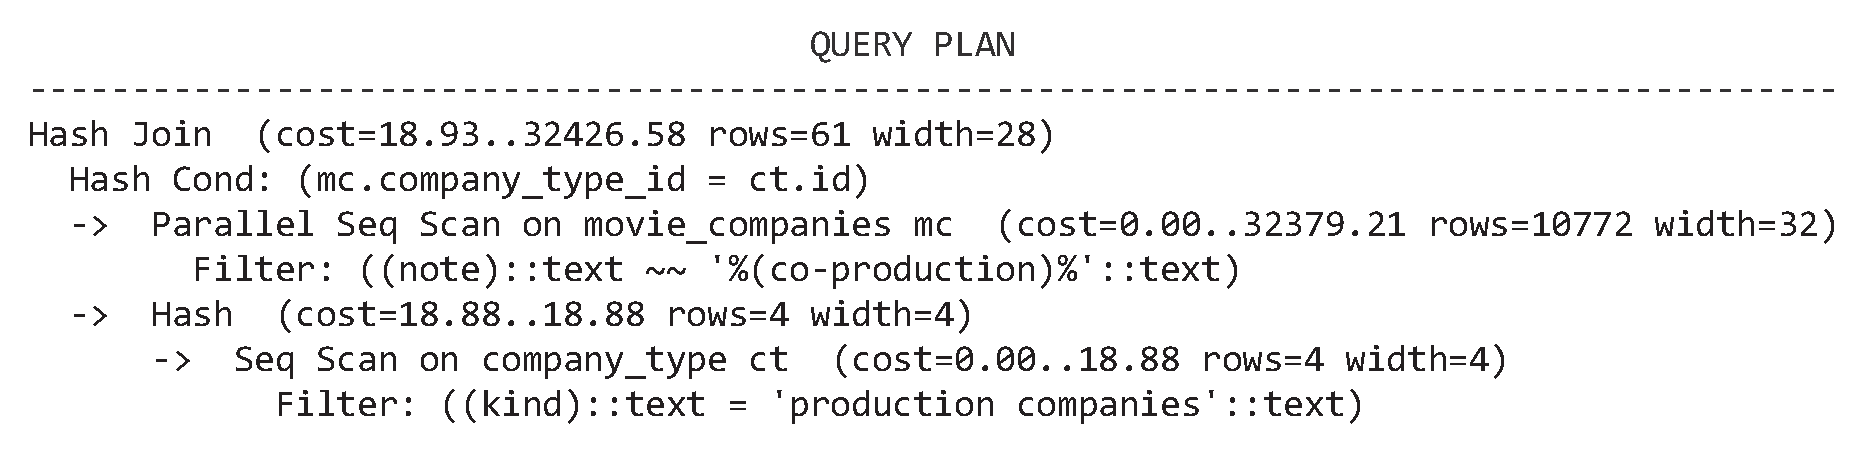
\includegraphics[width=0.45\linewidth]{newfig1.eps}
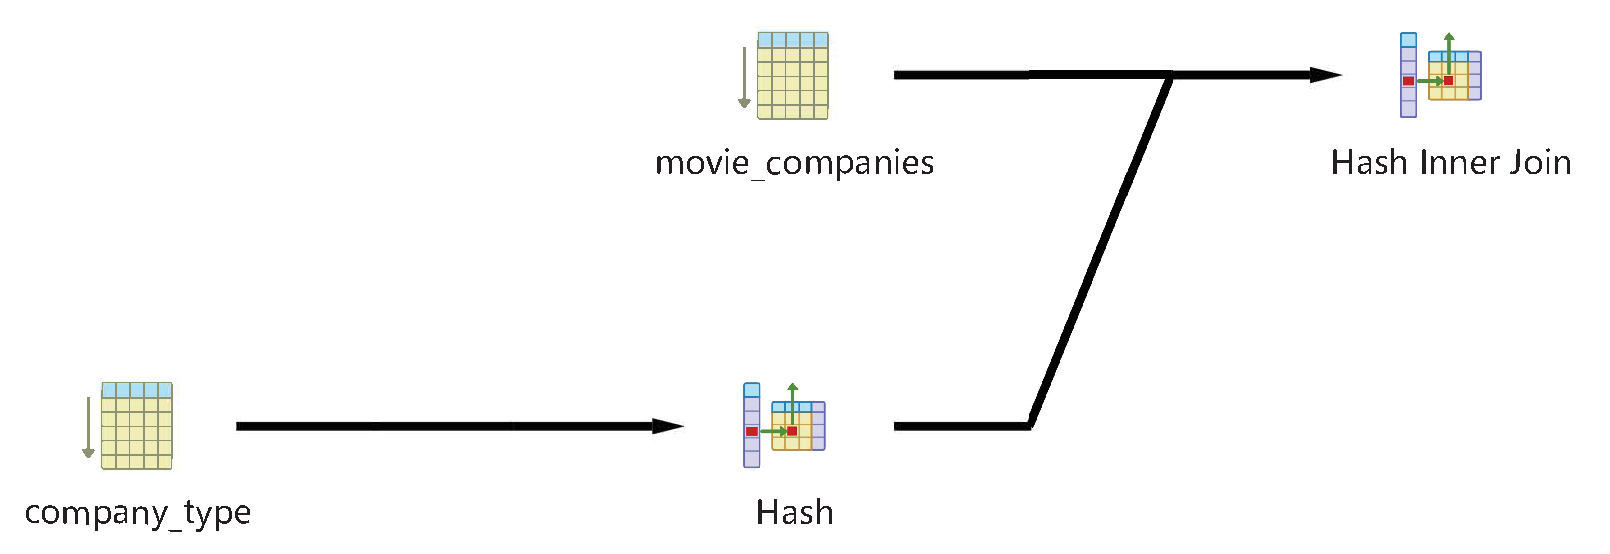
\includegraphics[width=0.5\linewidth]{sdf.eps}
\vspace{0ex}\caption{A \textsc{qep} in PostgreSQL and its visual tree representation.}
\label{fig:plan}
%\hrule
\vspace{0ex}\end{figure}


The majority of \textsc{nl} interfaces for \textsc{rdbms}~\cite{KS+20}, however, have focused either on translating natural language sentences to \textsc{sql} queries or narrating \textsc{sql} queries in a natural language. Scant attention has been paid for generating natural language descriptions of \textsc{qep}s~\cite{neuron,lantern}, which is a challenging problem.
Although deep learning techniques, which can learn task-specific representation of input data, are particularly effective for natural language processing, it has a major upfront cost. These techniques need massive training sets  of labeled examples to learn from. Such training sets in our context are prohibitively expensive to create as they demand database experts to translate thousands of \textsc{qep}s of a wide variety of \textsc{sql} queries.  Even  labeling using crowdsourcing is challenging as accurate natural language descriptions demand experts who understand \textsc{qep}s. Note that accuracy is critical here as low quality translation may adversely impact individuals' learning.

%====================================================================================================
\subsection{Learning Impact of Alternative Choices on QEP} \label{sec:impact}
%====================================================================================================
Natural language description of a \textsc{qep} enables a learner to understand the execution steps of a query. This may pique the interest of a learner to raise further questions related to query processing centred around a specific \textsc{qep}. Since major database textbooks typically discuss the adverse impact of choosing alternative physical operators or join ordering on the estimated cost, a learner may also like to delve deeper into the impact of these alternative choices on the estimated query processing cost of their queries.

\eat{This may be due to the shift from extrinsic motivation to intrinsic one to learn about relational query processing.}

\begin{example}  \label{eg:2} 
Reconsider Example~\ref{eg:1}. Doreen's course lectures and textbook discuss the impact of physical operator choices and join ordering  on the selection of a \textsc{qep}. Hence, after perusing the content of the \textsc{qep},  she wonders what will be the impact on the cost be if the hash join is replaced by a merge join? Is the estimated cost of the alternative query plan substantially higher compared to the \textsc{qep}? How much is the impact on the estimated cost if the join ordering is changed?   In this context, a narrative that explains why the \textsc{qep} is chosen by connecting its content with knowledge garnered from database textbooks will greatly benefit her learning. 
\EndOfProof
\end{example}

Unfortunately, as stated earlier, off-the-shelf \textsc{rdbms} are not developed for pedagogical support.  Typically, they do not expose the impact of alternative choices of various physical operators or join ordering on the \textsc{qep} in a \emph{user-friendly} manner to aid learning.  Note that such information is invaluable to learners as it not only facilitates hands-on inquire-driven learning on the impact of a choice of a physical operator  or a specific join ordering on the estimated cost of a \textsc{qep} but it also enables them to comprehend why a \textsc{qep} is chosen by the underlying \textsc{rdbms}. However,  an \textsc{rdbms} typically demands a learner to manually pose \textsc{sql} queries with various constraints on \textit{configuration parameters} (\textit{e.g.}, \texttt{enable\_hashjoin}, \texttt{enable\_nestloop} in PostgreSQL) to view the corresponding \textsc{qep} containing specific physical operators. Furthermore, one has to manually compare the generated plan with the original \textsc{qep} to understand the impact. Notably, a database course may not introduce these configuration parameters while exposing syntax and semantics of \textsc{sql}. It is also impractical to assume that learners will be familiar with them  when many are taking the course for the first time.  Clearly, based on the \textit{Expectancy-Value} and \textit{Flow} theories, a learner-friendly framework that can facilitate exploration of the impact of various physical operators and join ordering on a \textsc{qep} can greatly motivate learners to deeper engagement and learning of this topic. 

Intuitively,  given  an \textsc{sql} query and learner-specified \textit{preferences} (\eg merge join, index scan, specific join ordering), the goal is to automatically visualize the impact of these choices on the selected \textsc{qep}. In this context, it is important to generate a natural language-based explanation that goes beyond the conventional least-cost-based explanation to connect established knowledge related to usage scenarios of different physical operators from textbooks with the specified preferences. For instance, examples of some established knowledge are:  (a) index scan is the optimal access path for low selectivity whereas sequential scans perform better in high selectivity~\cite{borovicaGajic2018}; (b) merge join is preferred if the join inputs are large and are sorted on their join column~\cite{msdn}; (c) nested-loop join is ideal when one join input is small (\eg fewer than 10 rows) and the other join input is large and indexed on its join columns~\cite{msdn}. Such knowledge in the form of explanations will naturally facilitate learners' understanding of relational query processing. For instance, consider Example~\ref{eg:2}. Explanations such as (b) will help Doreen to understand why a hash join was chosen by the relational query engine.

The problem is challenging from several fronts. While under-the-hood it is straightforward to generate an \textsc{sql} query involving the learner-specified preferences and retrieve the corresponding \textsc{qep}, automatically generating appropriate visualization framework to aid learning is challenging. First, how should the results be presented in consistent with motivation theories to motivate learners to explore and learn? Note that a learner may want to view the impact of multiple physical operators and join ordering together instead of just a single operator or join ordering. Simply generating an \textsc{nl} description of the \textsc{aqp} is insufficient since this will demand a learner to manually compare the description of the original \textsc{qep} with it in order to understand the impact of various operators and join ordering. Naturally, this becomes tedious especially for complex queries.  Second, how can we generate  \textsc{nl} explanations that augment learning by connecting with textbook knowledge? It demands sophisticated text extraction, analytics, and summarization framework that connects the alternative query plans with relevant established knowledge embedded in online resources.   

%====================================================================================================
\subsection{Exploration of Informative Alternative Query Plans} 
%====================================================================================================
In the preceding challenge, a learner has clear preferences that they wish to explore with respect to a \textsc{qep}. However, this may not always be the case.  Some learners may not have clear idea of what alternative query plans they are interested in.\eat{ Consider the following example scenario.} 

\begin{example}\label{eg:3}
 Meng is another undergraduate student pursuing a degree in computer science and a classmate of Doreen in the database course. He also formulates the query in Example~\ref{eg:1}. After viewing the \textsc{qep}, he wonders what are the different alternative query plans (\textsc{aqp}s) considered by the underlying \textsc{rdbms} during the \textsc{qep} selection process. Specifically, are there alternative plan(s) that have similar (resp. different) structure and physical operators but very different (resp. similar) estimated cost? If there are, then how they look like? 
\EndOfProof
\end{example}


Off-the-shelf \textsc{rdbms} do not expose a \textit{representative} set of alternative query plans considered by the underlying query optimizer during the selection of a \textsc{qep} in a \emph{user-friendly} manner to aid learning. Hence, due to the lack of easy access to such information in \textsc{rdbms}, based on the \textit{Expectancy-Value Theory}, learners may restrict themselves to the simple and limited number of examples that are typically exposed in textbooks and lectures or simply abandon the effort. Clearly, a learner-friendly framework that can facilitate retrieval and exploration of ``informative'' alternative query plans associated with a given query can greatly aid in answering Meng's questions related to the query optimization process. 

Selecting a set of \textit{informative} \textsc{aqp}s to facilitate learning is a technically challenging problem. First, what is an ``informative'' \textsc{aqp} in the context of learning? To elaborate further, reconsider Example~\ref{eg:3}. Figures~\ref{fig:alter_plans}(b)-(c) depict two alternative plans for the query where the physical operator/join order differences are highlighted with red rectangles and significant cost differences are shown using yellow nodes. Specifically, \textit{AP1} has very similar structure as the \textsc{qep} but different join order involving \texttt{title} and \texttt{company\_type} relations and significantly different estimated cost. \textit{AP2}, on the other hand, displays similar estimated cost as the \textsc{qep}  but different join order. \textit{Which of these alternative plans should be revealed to Meng?} The overarching goal here is to  choose alternative plan(s)  that may enhance Meng's knowledge of the \textsc{qep} selection process (\ie informative) as well as motivate him to learn and explore. Certainly, any \textit{informativeness} measure needs to be cognizant of plans that a learner have already viewed for her query (including the \textsc{qep}) in order to avoid the exposure of highly similar information. It should also facilitate retrieval of plans that learners may be interested in as far as query optimization is concerned. Hence, it is paramount to take feedback from learners on the \textit{types} of \textsc{aqp}s that are potentially of interest to them and devise a mechanism to quantify \textit{informativeness} of a plan by mapping the knowledge acquired from the feedback to a \textit{utility} measure. Subsequently, we need to design techniques that can select informative plans that  \textit{maximize} the \textit{utility} as we cannot simply rely only on the estimated cost of alternative plans.  Second, the number of candidate \textsc{aqp}s for a given \textsc{sql} query is exponential in the worst case~\cite{SC98}. Hence, it is prohibitively expensive to scan all these plans to select informative ones. Note that the selection of \textsc{aqp} cannot be integrated into the plan enumeration step of the underlying query optimizer. We need to know the \textsc{qep} when computing \textsc{aqp} as they are selected with respect to the \textsc{qep} a learner has seen. 
	
At first glance, it may seem that we can select $k>1$ alternative query plans where $k$ is a value specified by a learner. Although this is a realistic assumption for many top-$k$ problems, learners may not necessarily be confident to specify the value of $k$ always. They may prefer to \textit{iteratively} view one plan-at-a-time and only cease exploration once they are satisfied with the understanding of the query optimization process for a specific query. Hence, $k$ may not only be unknown \textit{apriori} but also the selection of an \textsc{aqp} at each iteration to enhance learning of different plan choices depends on the plans viewed by a learner thus far. Clearly, it does not increase learners' understanding of the query optimization process or motivate them to use the framework if a plan with highly similar information of an already viewed plan is revealed to them in the subsequent iterations. This demands for a flexible solution framework that can select informative \textsc{aqp}s in absence or presence of the $k$ value. 


%====================================================================================================
\subsection{Understanding Cost Estimation of a Physical Query Plan}  \label{sec:cost}
%====================================================================================================
The preceding subsections introduce research issues that aim to facilitate learning of the execution strategy of an \textsc{sql} query and  interesting plan choices a relational query optimizer makes in practice. Another key knowledge that a learner needs to acquire is the cost estimation procedure of these plans.   

\begin{example}\label{eg:4}
 Doreen and Meng have learnt from textbooks and lectures how the cost of a physical query plan can be estimated. However, the number of queries considered in these modes of learning and their complexities are limited. They are motivated to experience cost estimation of plans associated with a wider variety of queries. Hence, they pose several queries with different degrees of complexity on the IMDb dataset in PostgreSQL. They can view the overall estimated cost of a \textsc{qep} as well as cost of different subtrees (\eg Figure~\ref{fig:alter_plans}). However, they cannot view step-by-step details of the input parameters and the formulas used by the underlying query optimizer to compute these numbers. For instance, in Figure~\ref{fig:alter_plans}(a), why is the cost of the first \texttt{HASH JOIN} \textit{2046.6}? By undertaking a back-of-the-envelope calculation using formulas learnt in the course, they could not replicate this value. Are some of the principles and formulas to compute cost different from what they have learnt from textbooks and lectures? If so, then why? 
 
 Doreen and Meng also wonder what the intermediate result sizes of different operations are here? When they execute one of the queries, they have to wait for a considerable amount of time to view the results. Does the estimated time cost of the \textsc{qep} differ significantly from the actual cost? Why? 
\EndOfProof
\end{example}

Existing \textsc{rdbms} do not provide any learner-friendly support to facilitate such learning. Consequently, based on motivation theories, learners may not pursue this direction of inquiry using an \textsc{rdbms}, surrendering valuable opportunity for hands-on acquisition of knowledge of the cost estimation process. It is challenging, however, to expose an interface to facilitate such learning and exploration. First, it demands automated analysis of the code base of the underlying query optimizer to extract various formulas used for cost estimation. These formulas may not necessarily be identical across all \textsc{rdbms} or textbooks. For instance, in~\cite{dbtext}, the cost of a selection involving inequality condition is approximated to be 1/3 of the input size independent of the selection condition. On the other hand, in~\cite{cow}, more accurate measure is used for estimating the selection cost.  Furthermore, a specific \textsc{rdbms} may implement variants of these formulas. Second, it is paramount to connect these formulas with specific input parameters for a query to reveal how the cost of a plan is estimated while emphasizing the similarity and differences with textbook knowledge. A framework that can support this in a palatable manner to facilitate learning is non-trivial as it may demand a sophisticated natural language generation framework that connects analysis of the code base with textbook content. Third, superior visualization and \textsc{nl}-based framework are necessary to explain to learners the reasons for the differences in estimated and actual cost of a query. Although tools such as~\cite{picasso} allow one to visualize the cost of different plans over the plan space,  they are not designed for explaining the \emph{cost differences} for a \emph{specific} query in a palatable manner. 

%====================================================================================================
\subsection{A Unifying Framework: Chatting with a Relational Query Engine} 
%====================================================================================================

\begin{figure}[t]
\centering
\includegraphics[width=\linewidth]{chatbot.pdf}
\vspace{0ex}\caption{An example of interaction between a learner and the chatbot.}
\label{fig:chatbot}
%\hrule
\vspace{0ex}\end{figure}

Although addressing the aforementioned issues has the potential to facilitate learning of relational query processing by providing learner-friendly platforms, a set of isolated platforms that address these different issues will make it cumbersome for learners to navigate and take advantage of them.  For instance, learners may find it overwhelming to operate three independent technology-enabled learning platforms targeting \textsc{nl} description generation of \textsc{qep}, exploration of \textsc{aqp}, and cost analysis of query plans, respectively. This may deter them to use such technology for learning. Given that young adults often interact through chat apps (\eg Whatsapp, WeChat), a natural language interaction framework (\ie chatbot) that can unify these solutions may bring practical benefits to learners.  A possible interaction between a learner and a hypothetical chatbot designed for interacting with a relational query engine are shown in Figure~\ref{fig:chatbot}.

Building a high-quality chatbot for a relational query engine to facilitate learning is non-trivial and challenging.  In addition to the challenges mentioned earlier for addressing individual components, a chatbot brings new challenges with respect to correct parsing and interpretation of a learner's statement, constructing correct (syntactically and semantically) responses in a natural language, engaging learners in conversations, and so on. While these challenges are long recognized in building a generic chatbot~\cite{GGL18}, the domain-specific nature of the problem brings in interesting flavor to it. Different from natural conversations, a learner’s questions usually have concrete objectives, actively requesting information, and an answer to every question should facilitate understanding of relational query processing. Furthermore, a learner's questions at each step are not only closely related to the chatbot’s current answers, but also need to take into account the context of the previous parts of the conversation. For example, consider the first three questions in Figure~\ref{fig:chatbot} from the learner. These questions are actively requesting information related to relational query processing. Observe that the third question is related to the preceding parts of the conversation.  

Any chatbot needs to consider two kinds of information in a learner's question: (1) the intent of the question (\eg understanding cost computation) and (2) the content of the question (\eg cost computation steps of zigzag join in a \textsc{qep}).  To this end, we can construct a \textit{query processing knowledge graph} semi-automatically to represent a collection of relational query processing concepts. Then the intent and content can be determined by \textit{mapping} the question to different concepts in the knowledge graph. Note that similar idea of knowledge graph has been recently exploited in the context of question generation for multi-party court debates for judicial education~\cite{ZJ+22}. Once the intent and content of a question are determined, the chatbot invokes the relevant component (Section~\ref{sec:nlg}-\ref{sec:cost}) to retrieve the answer for the specific question. The result returned by it is then \textit{transformed} into a natural language (supported by visual representations, if necessary) and presented to the learner.

   

  \begin{table*}[t]
\centering
 \caption{\label{tab:learn}Learning-centric issues.}
 \scriptsize
 \begin{tabular}{|p{70mm}|p{77mm}|}
  \hline
  \textbf{Issue} & \textbf{Questions to address}  \\
  \hline
 \textbf{ \textit{Rational for the impact of technologies on learning}} & Will learners work more efficiently, more effectively, more intensely? \\
 & Will the technology help them to learn for longer, more deeply, more productively? \\ \hline
\textbf{\textit{Role of technology in learning}} & Will it help learners to gain access to learning content? \\
& Will the technology provide feedback?\\ \hline
 \textbf{\textit{Technology should support effective interaction for learning}} & Does it support effective interaction with learners?\\ \hline
 \textbf{\textit{Identify what learners will stop doing}} & What it will replace or how the technology activities will be additional to what learners would normally experience?\\
  \hline
 \end{tabular}
\end{table*}
 
%====================================================================================================
\subsection{Learning-centric, Generic, and Psychology-Awareness of Solutions}  \label{sec:issue}
%====================================================================================================
In addition to the challenges within each aforementioned issues, any solution to them must ensure the following features.

\begin{itemize} \itemsep = -0.5ex

\item \textbf{Learning-centric.} The role, impact, and interaction of the platforms designed to address aforementioned issues have to be learning-centric, \ie they bring about improvement in learning. Table~\ref{tab:learn} lists the learning-centric issues~\cite{HXK12} that any technology-enabled solution needs to address. For instance, consider the last issue. An effective solution to \textsc{nl} descriptions of \textsc{qep}s will provide learners an additional interface to learn about query execution strategies to what they would normally experience. Similarly, consider the second issue. A solution to user-friendly exploration of \textsc{aqp}s will enable learners to gain easy access to informative plans to aid learning of the query optimization process. 
 
\item \textbf{Generalizability.}  Solutions must be \textit{generalizable} to different \textsc{rdbms} and applications. This will significantly reduce the cost of its deployment in different learning institutes and environments where different application-specific examples and \textsc{rdbms} may be used to teach database systems. For example, the natural language generation framework should be generalizable.  Ideally we would like to generate natural language descriptions of \textsc{qep}s using one application-specific dataset (\eg movies) and then use it for other applications (\eg hospital) on any off-the-shelf \textsc{rdbms}. 

\item  \textbf{Psychology-awareness.} Any technology-enabled learning framework has to be \textit{learner-centric}, \ie it has to be cognizant of the psychology of learners. Any deployable  solution has to be palatable and engaging to learners so that they are motivated to learn and explore. Hence, these solutions need to be consistent with various cognitive psychology and motivation theories to have practical impact. For example, the \textsc{nl} descriptions for different queries must not use the same language to describe various operations in \textsc{qep}s. Similarly, highly similar \textsc{aqp}s should not be exposed to the learners. Otherwise, learners may feel bored after viewing several \textsc{aqp}s or reading the \textsc{nl} descriptions for several queries. In fact, this is consistent with research in psychology that have found that repetition of messages can lead to annoyance and boredom~\cite{CP79} resulting in purposeful avoidance~\cite{HK13}, content blindness~\cite{HG+11}, and even lower motivation~\cite{SPC90}.
\end{itemize}


%====================================================================================================
\subsection{Towards Data-driven Education} 
%====================================================================================================
As remarked in Section 1, learning can be facilitated  by education. Hence, technological platforms that address the aforementioned challenges may pave the way for \emph{data-driven} education due to rich access to \textit{interaction log} data of learners.  Such log data may consists of access times of learners, history of queries formulated by learners, temporal information related to various interactions, among others. This provides a rich data source for building data-driven techniques to facilitate education by analyzing these data at both individual and group levels and correlating them with the performances of learners in tests (\ie academic outcomes).  A non-exhaustive list of questions that can be answered by exploiting the log data to facilitate data-driven education is as follows:

\begin{itemize} \itemsep = -0.5ex

\item How do the type and complexity of \textsc{sql} queries posed by learners evolve over time? What are the activity patterns of learners during a semester? Answers to these questions may provide insights on motivation and learning habits of learners.  

\item How do learners learn relational query processing? Numerous studies in cognitive psychology show that \textit{spacing} (\ie distributing practice over more sessions) significantly improves long-term learning compared to \textit{massing} (\ie practice in longer sessions)~\cite{BB11,BDK13,SB15,TR10}. The interaction data may enable us to build models to predict learners demonstrating massing, thereby enabling timely intervention to nudge them to more effective learning habits.

\item Research in education posits that technology can be used effectively as a short but focused intervention to improve learning especially when there is regular and frequent usage over a period of several weeks~\cite{HXK12}. In our context, it is expected that the platforms are also for focused usage over a period of few weeks. Do they help learners to perform better in tests and coursework? Is there any correlation between frequency of engagement with a platform and performance? Answer to this may provide data-driven insights to the effectiveness of these tools in learning. 

\item Do learners continue to use the platforms even after the end of a database course? This may indicate intrinsic motivation to learn relational query processing. 

\item Can the queries posed by learners over time shed light on the difficulties they face with respect to the learning and understanding of relational query processing and optimization? Answer to this question may facilitate the design of more effective and efficient pedagogical strategies to improve effectiveness of teaching.


\end{itemize} 

In summary, addressing the aforementioned research issues provide us a unique opportunity to take a data-driven approach to the education of relational query processing that may otherwise be infeasible through traditional mode of teaching.

\begin{figure}[t]
\centering
\includegraphics[width=0.4\linewidth]{truss.png}
\includegraphics[width=0.5\linewidth]{neuron-time.png}
\vspace{0ex}\caption{(a) Architecture of \textsc{truss} (left); (b) No. of queries versus time (right).}
\label{fig:neuron}
%\hrule
\vspace{0ex}\end{figure}


%====================================================================================================
\section{The TRUSS System}  
\label{sec:truss}
%====================================================================================================
 Figure~\ref{fig:neuron}(a) depicts the high-level architecture of the \textsc{truss} (\textbf{T}echnology-enabled Lea\textbf{R}ning of Q\textbf{U}ery Proce\textbf{SS}ing) system that we are currently building to address the challenges introduced in the preceding section.  The \textit{QEP-to-NL Generator}, \textit{Alternative Plan Explorer}, and \textit{Cost Explainer} components aim to address the challenges in Sections 3.2, 3.3 \& 3.4, and 3.5, respectively. The \textit{Conversation Manager} is to realize the unifying chatbot (Section 3.6) and the \textit{Learner Interaction Manager} is responsible to facilitate data-driven education (Section 3.8). In this section, we briefly describe our recent efforts to build three frameworks, \textsc{neuron}~\cite{neuron} and \textsc{lantern}~\cite{lantern-demo}, that aim to address the problem described in Section~\ref{sec:nlg} (\ie \textit{QEP-to-NL Generator}), and \textsc{mocha}~\cite{mocha} that takes an initial step to address the problem in Section~\ref{sec:impact} (\ie  \textit{Alternative Plan Explorer}).  The reader may refer to~\cite{neuron,lantern,lantern-demo,mocha} for details on these frameworks.
%====================================================================================================
\subsection{NEURON and LANTERN} %17
%====================================================================================================
\textsc{neuron}~\cite{neuron,neuron-soft} is the first system that exploits a rule-based interpretation engine to generate \textsc{nl} description for \textsc{qep} in PostgreSQL.  Specifically, given the \textsc{qep} of a \textsc{sql} query, \textsc{neuron} first parses and transforms the \textsc{qep} of an \textsc{sql} query into an operator tree where each node contains relevant information associated with a plan (\eg filter conditions). Next, it traverses the tree and generates a \textsc{nl} description of the node based on \textsc{nl} templates and the information it carries.  It also supports a preliminary \textit{natural language question answering}  system that allows a user to seek answers to a variety of concepts and features associated with a \textsc{qep}. 

\textsc{neuron} is a rule-based framework that is tightly integrated with PostgreSQL. Hence, it is not generalizable (Section~\ref{sec:issue}).  \textsc{lantern}~\cite{lantern,lantern-demo,lantern-soft} addresses this limitation by not only making the solution generalizable but also psychology-aware. It incorporates a \textit{declarative framework} called \textsc{pool} to empower \textit{subject matter experts} (\textsc{sme}s) create and manipulate the \textsc{nl} descriptions (\ie labels) of physical operators, which are the building blocks of \textsc{qep}s. The data definition in \textsc{pool} allows one to declaratively create physical operator objects associated with a specific \textsc{rdbms}. For example, one can create the definition of hash join operator in PostgreSQL (\texttt{pg}) as follows.

\begin{quote}
\begin{verbatim}
CREATE POPERATOR hashjoin FOR pg
(ALIAS = null,
TYPE = 'binary',
DEFN = null,
DESC = 'perform hash join',
COND = 'true',
TARGET = null)
\end{verbatim}
\end{quote}

In particular, the \texttt{TYPE} attribute can take either \textsf{`unary'} or \textsf{`binary'} value. The \texttt{DESC} attribute allows one to specify a natural language description of the operation performed by the operator.   The \texttt{COND} attribute takes a Boolean value to indicate whether a specified condition (\eg join condition) should be appended to the natural language description of an operator. Values of all attributes are taken from the atomic type \texttt{string} (possibly empty). Note that no relation or condition is specified in \texttt{DESC}. This is because these are added automatically to \texttt{DESC} by exploiting \texttt{TYPE} and \texttt{COND} attributes  of an operator. For instance, since \texttt{TYPE} is \textsf{`binary'} in the above definition, two variables representing join relations will be added automatically to the description of \texttt{hashjoin}.  Lastly, the \texttt{TARGET} attribute allows one to specify the operator name which is supported by the defined operator. For example, \texttt{TARGET} is set to \textsf{`hash join'} for the definition of \texttt{hash} operator.


The key goals of the data manipulation component of \textsc{pool} are to provide syntactical means to support (a) retrieval of specific properties (\ie attributes) of physical operators using \textsc{sql}-like \texttt{SELECT-FROM-WHERE} syntax, (b) generation of the \textit{template} for natural language description of  an operator using the \texttt{COMPOSE} clause, and (c) update properties of physical operator objects using  \texttt{UPDATE} and \texttt{REPLACE} clauses. Specifically, the \texttt{COMPOSE} clause uses the \textit{desc}, \textit{type}, and \textit{cond} attributes of operators to generate the template. For example, the template generation for the \texttt{hash} operator can be specified as follows.
\begin{quote}
\begin{verbatim}
COMPOSE hash FROM pg
\end{verbatim}
\end{quote}

The above statement will return the template \textit{``hash \$$R_1$\$''}, which can be subsequently used by \textsc{lantern} to generate specific description of the \texttt{hash} operator in a \textsc{qep}. Also, observe that $R_1$ is appended based on the \textit{type} attribute of the \texttt{hash} object. An example to generate the \textsc{nl} description template of the \texttt{hash join} operator is as follows.
\begin{quote}
\begin{verbatim}
COMPOSE hash, hashjoin FROM pg
USING hashjoin.desc = 'perform hash join'
\end{verbatim}
\end{quote}
The above statement generates the following template: \textit{``hash \$$R_1$\$ and perform hash join on \$$R_2$\$ and \$$R_1$\$ on condition \$$cond$\$''}. 

The update statement can be exploited to assign definition or description of an operator from one commercial database to another, thereby making it more efficient for an \textsc{sme} to specify properties of physical operators. The following example demonstrates how the description of hash join in PostgreSQL is transferred to the hash join operator in DB2.

\begin{quote}
\begin{verbatim}
UPDATE db2
SET desc = (SELECT desc
 FROM pg WHERE pg.name = 'hashjoin')
WHERE db2.name = 'hsjoin'
\end{verbatim}
\end{quote}

It can also be used along with the \texttt{REPLACE} clause to transfer definition or description of an operator object to another within the \emph{same} source. For example, one can transfer the description of hash join to nested loop join by replacing the word \textsf{`hash'} with \textsf{`nested loop'} as follows.

\begin{quote}
\begin{verbatim}
UPDATE pg
SET desc = REPLACE((SELECT desc FROM pg AS pg2
WHERE pg2.name = 'hashjoin'), 'hash', 'nested loop')
WHERE pg.name = 'nested loop join'
\end{verbatim}
\end{quote}

Note that the \texttt{REPLACE} clause takes three parameters as input, namely, the description or definition of an operator object, the string in it that needs to be replaced (\eg \textsf{`hash'}), and its new replacement string (\eg \textsf{`nested loop'}).

Once the physical operator objects for different \textsc{rdbms} are created in \textsc{pool} and stored, the physical operator tree of a given query in any \textsc{rdbms} can be augmented by automatically annotating relevant nodes with \textsc{nl} descriptions by leveraging the \texttt{COMPOSE} statement and replacing the place holders in \textsc{nl} templates with specific relations, attribute names, and predicates relevant to the query.  The \textsc{nl} description generation framework then utilizes this augmented operator tree and \textit{integrates} a rule-based and deep learning-based techniques. In particular, the latter infuses language variability in the descriptions opportunely. This strategy has been shown to mitigate the impact of boredom on learners that may arise due to repetitive statements in different \textsc{nl} descriptions~\cite{lantern}.
%====================================================================================================
\subsection{MOCHA} %17
%====================================================================================================
\textsc{mocha} (i\underline{M}pact of \underline{O}perator \underline{CH}oices visu\underline{A}lizer)~\cite{mocha, mocha-soft} aids learner-friendly interaction and visualization of the impact of alternative physical operator choices on a selected \textsc{qep} for a given \textsc{sql} query. It is built on top of PostgreSQL. Given  an \textsc{sql} query and learner-specified \textit{operator preferences} (\eg merge join, index scan), \textsc{mocha} automatically visualizes the impact of these choices on the selected \textsc{qep}.
Specifically, it exploits the \textit{planner method configuration}\footnote{\scriptsize \url{www.postgresql.org/docs/9.2/runtime-config-query.html\#RUNTIME-CONFIG-QUERY-CONSTANTS}.} feature of PostgreSQL to generate \textsc{aqp}s based on a user input. The configuration parameters in this feature provide a way to enforce the query optimizer to choose a query plan with certain user-specified physical operators. By default, all parameters are turned on during query processing. A query request is sent to PostgreSQL using the default settings to retrieve the \textsc{qep} of a query. 

In order to retrieve \textsc{aqp}s, a learner may select a subset of the configuration parameters (through a user-friendly visual interface) based on the physical operators that she intend to view in these plans. In this case, the corresponding parameters are set to \textsf{``true"} (\eg \texttt{SET enable\_mergejoin = \textsf{true}}) in the query request. \textsc{mocha} supports two modes for generating alternative plans, namely, \textit{single mode} and \textit{multiple mode}.  In the former mode, \textsc{mocha} sends a query request to PostgreSQL in which the \emph{unselected} parameters are set to \textsf{``false''} to generate an \textsc{aqp} containing the operators corresponding to the selected parameters that are relevant to the processing of the query. In the latter mode, every selected parameter is either set to \textsf{``true''} or \textsf{``false''} to create all possible combinations of these parameters. \textsc{mocha} iterates through these combinations and sends corresponding query requests to PostgreSQL. It only maintains all \emph{distinct} plans retrieved from these requests. To facilitate learning, it provides a learner-friendly \textsc{gui} to detect and visualize various structural and cost differences between a selected \textsc{aqp} and the \textsc{qep}. 

\textsc{mocha} also generates a natural language-based explanation that goes beyond the conventional least-cost-based explanation to connect established knowledge related to usage scenarios of different physical operators that a learner has learnt from textbooks with the operators in a \textsc{qep}. The current version manually extracts usage scenarios of different physical operators from the relevant literature. This is feasible since there is a small number of physical operators in PostgreSQL. Then a set of documents containing these usage scenarios is indexed using an inverted index where each document is associated with a single physical operator.
For a given \textsc{qep}, it identifies relevant operators and retrieves associated predicates and join conditions, if any. The text explanation is then generated for an operator by utilizing a rule-based template, the inverted index to retrieve corresponding usage scenario,  and database statistics information (\eg selectivity).  The generated explanation is visually displayed on the visual interface of \textsc{mocha}. For example, an explanation could be \textit{``the \textsc{qep} uses index scan on the \texttt{lineitem} table as it is faster due to the high selectivity of the predicate (\ie \texttt{l\_orderkey = orders.o\_orderkey})''}. 

In the future, we intend to generalize \textsc{mocha} to accommodate major \textsc{rdbms}, support visualization of the impact of join ordering, and automate the manual extraction of usage information of various physical operators in these \textsc{rdbms}. More importantly, we wish to deploy \textsc{mocha} in our learning environment and investigate its impact on students taking the database systems course.

%====================================================================================================
\subsection{Usage and Impact of NEURON}
%====================================================================================================
\textsc{neuron} and \textsc{lantern} are currently deployed in database systems courses in NTU and Xidian University. We now briefly describe our initial efforts to measure \textsc{neuron}'s impact on the learning  of \textsc{qep}. To this end, we introduced it to students taking the undergraduate database systems course (\textit{CZ4031}) in NTU in the August semester of 2021. 166 students were enrolled in this course. These students are  pursuing a variety of degrees such as computer science, computer engineering, data science and analytics, and business and computing. In particular, the topic of query processing and optimization was covered in 4 weeks (September-October) over eight 1-hour lectures. On October 28th, the students took a test on the topic of query processing and optimization. The following message was sent to the students on 14th October, 2021: \textit{``If you wish to understand query execution plans (\textsc{qep}) generated by PostgreSQL for different \textsc{sql} queries, you may use the software called \textsc{neuron} at \url{https://neuron.scse.ntu.edu.sg/}. \textsc{neuron} translates the \textsc{qep} of a query to natural language description.'' }  We did not nudge students any further on using \textsc{neuron} or give them any hints on whether questions related to natural language descriptions of query plans will appear in the test. Hence, students were not aware of any assessment-related rewards if they used the tool. The goal here is to observe whether learners will use it without any nudging or grades-related rewards and whether they will benefit from it.

\begin{figure}[t]
\centering
\includegraphics[width=0.7\linewidth]{neuron-no-query.png}
\vspace{0ex}\caption{No. of queries versus no. of users.}
\label{fig:query}
%\hrule
\vspace{0ex}\end{figure}

We observe the usage of \textsc{neuron} from 14th October to 2nd December by analyzing the log file. Note that 12th November was the last date of the course culminating with the submission of a course project. Since a user needs to access \textsc{neuron} by logging using an email address, we were able to match majority of the email addresses that accessed it with those registered for the course. There were 69 distinct learners (41.5\%) using \textsc{neuron} during this period. Figure~\ref{fig:neuron}(b) reports the number of queries posed by learners over time. In total, 888 valid \textsc{sql} queries (484 distinct queries) were executed on \textsc{neuron}. The distribution of the number of queries versus the number of distinct learners who posed that number of queries is shown in Figure~\ref{fig:query}. Observe that more than 85\% of them posed more than one query and the maximum number of queries posed by a single user is 93! Prior to October 28th (test date), the number of distinct users is 48 and the number of queries posed is 409 (211 distinct queries). Hence, the usage of \textsc{neuron} continued even after the test as learners may be using it to understand \textsc{qep}s for their project work. Some students used it even after the official end date of the course probably demonstrating intrinsic motivation to explore \textsc{qep}s. 

To investigate whether \textsc{neuron} may benefit learners to understand \textsc{qep}, we use the test as a proxy. In the test, a question was specifically set to this end. The students were asked to explain in natural language the visual format of a \textsc{qep}  (in PostgreSQL) for an \textsc{SQL} query on IMDb database involving two joins, scans, and sort operations. The question carried 10 marks. Observe that it matches very closely to \textsc{neuron}'s goal. This enables us to evaluate more accurately possible impact of \textsc{neuron} on the test performance.  

 In order to avoid any bias, a teaching assistant (TA) who is not involved with \textsc{neuron} graded the answers to this question.  The TA was given the solution and was allowed to set the marking scheme for the question. The number of students who took the test is 162. The average score of students who used (resp. not used) \textsc{neuron} prior to test is 8.43 (resp. 7.07). The maximum, minimum, and median scores of these two groups are (10, 6.5, 8) and (10, 0, 7.5), respectively. Among the non-\textsc{neuron} users, the percentage of students with scores lower than the minimum score in the \textsc{neuron} user group (\ie 6.5)  is 21.31\%.  Furthermore, the percentage of \textsc{neuron} users (resp. non-\textsc{neuron} users) with scores higher than the average score of 8 is 47.5\% (resp. 35.25\%). Some of the common errors made by students are (a) not describing in natural language; (b) incorrect sequence of steps; (c) not including filter conditions in the scan operations; and (d) unclear specifications of operators and intermediate results. Observe that these errors could have been mitigated with the usage of \textsc{neuron}.

 In summary, while we cannot infer causal link from the initial results, it is possible \textsc{neuron} may improve learning of query execution strategies. We are still in the early stages of understanding the impact of this tool on learning. We intend to use \textsc{neuron} and \textsc{lantern} in future semesters to gather sufficient longitudinal data for a more detailed investigation of technology-enabled learning and their impact on data-driven education.

%====================================================================================================
\section{Conclusions}
\label{concl}
%====================================================================================================
Impact of digital technologies on learning has consistently shown positive benefits when they are aligned.  With the advent of data science and lifelong learning, there has been growing interest in the database course from adult learners with diverse background. This necessitates us to revisit the traditional way we teach this course by supplementing it with technological support to improve learning. This paper contributes a vision of technology-enabled learning of the topic of relational query processing in a database systems course. Specifically, our vision attempts to carve out a substantially new research topic that is at the intersection of learning sciences and data management to improve learning of relational query processing.  To the best of our knowledge, this vision has not been systematically investigated before, prior to our recent publications.

\vspace{1ex}\noindent\textbf{Measures of success.} Successful realisation of this vision will improve learning and understanding of the complex topic of relational query processing. But several non-trivial and novel research challenges as articulated in the paper need to be overcome to realize  it. Adoption of the potential solutions by real-world learners as a supplement to traditional modes of learning will be another measure of success.

\vspace{1ex}\noindent\textbf{Wider applicability.} We focused on the topic of relational query processing since it is one of the most challenging topic in a database systems course. Nevertheless, it is easy to see that our vision of technology-enabled learning can be extended to other topics such as enabling technologies to facilitate learning of \textsc{sql} queries.


\begin{thebibliography}{10}
	\itemsep=1pt
	\begin{small}
	
	\bibitem{imdb} The IMDb database. \url{https://relational.fit.cvut.cz/dataset/IMDb}.
	
	\bibitem{msdn} Advanced query tuning concepts. \url{https://docs.microsoft.com/en-us/previous-versions/sql/sql-server-2008-r2/ms191426(v=sql.105)?redirectedfrom=MSDN}, 2012.
	
	\bibitem{lantern-soft} \textsc{lantern} software. \url{https://howardlee.cn/lantern/}.
	
	\bibitem{mocha-soft} \textsc{mocha} software. \url{https://howardlee.cn/mocha/}.
	
	\bibitem{neuron-soft} \textsc{neuron} software. \url{https://howardlee.cn/#/}.

\bibitem{unesco} USESCO Insititute of Lifelong Learning. UNESCO Global Network of Learning Cities. Accessible at \url{https://uil.unesco.org/lifelong-learning/learning-cities}, 2019.

\bibitem{AP12} E. M. Anderman, H. Patrick. Achievement goal theory, conceptualization of ability/intelligence, and classroom climate. \textit{In Handbook of research on student engagement},  Springer: Boston, MA, 2012.

\bibitem{BC+15} A. Bhangdiya, B. Chandra, B. Kar, B. Radhakrishnan, K. V. M. Reddy, S. Shah, S. Sudarshan.
The XDa-TA system for automated grading of SQL query assignments. \textit{In ICDE}, 2015.

\bibitem{BB11} E. L. Bjork, R. Bjork.  Making things hard on yourself, but in a good way. \textit{Psychology in the Real World}, 59-68, 2011.

\bibitem{BDK13} R. A. Bjork, J. Dunlosky, N. Kornell. Self-regulated learning: Beliefs, techniques, and illusions. \textit{Annual review of psychology}, 64, 417–444, 2013.

\bibitem{borovicaGajic2018} R. Borovica-Gajic, S. Idreos, A. Ailamaki, M. Zukowski, C. Fraser. Smooth scan: robust access path selection without cardinality estimation. \textit{The VLDB Journal}, 27(4):521-545, 2018.

\eat{\bibitem{BCR09} N. Bruno, S. Chaudhuri, R. Ramamurthy. Interactive plan hints for query optimization.\textit{ In SIGMOD}, 2009.}

\bibitem{CP79} J. T. Cacioppo and R. E. Petty. Effects of Message Repetition and Position on Cognitive Response, Recall, and Persuasion. \textit{Journal of Personality and Social Psychology} ,37, 1: 97-109, 1979.

\bibitem{SC98} S. Chaudhuri. An Overview of Query Optimization in Relational Systems. \textit{In PODS}, 1998.

\bibitem{lantern-demo} P. Chen, H. Li, S. S. Bhowmick, S. R. Joty, W. Wang. LANTERN: Boredom-conscious Natural Language Description Generation of Query Execution Plans for Database Education.\textit{ In SIGMOD}, 2022.

\bibitem{DG11} J. Danaparamita, W. Gatterbauer. QueryViz: Helping Users Understand SQL Queries and Their Patterns. \textit{In EDBT}, 2011.

\bibitem{DV+91} E. L. Deci, R. J. Vallerand, L. G. Pelletier, R. M. Ryan. Motivation and education: The self-determination perspective. Educational psychologist, 26(3-4), 325-346, 1991.

\bibitem{dbtext} H. Garcia-Molina, J. D. Ullman, J. Widom. Database Systems: The Complete Book. \textit{Prentice-Hall}, 2002.

\bibitem{GK12} M. Gawade, M. L. Kersten. Stethoscope: A platform for interactive visual analysis of query execution plans . \textit{PVLDB}, 5(12), 2012.

\bibitem{Gross} R. Gross. Psychology: The Science of Mind and Behaviour. \textit{Hachette UK}, ISBN 978-1-4441-6436-7.

\bibitem{GGL18} J. Gao, M. Galley, L. Li. Neural Approaches to Conversational AI. \textit{In ACL}, 2018.

\bibitem{picasso} J. R. Haritsa.  The Picasso Database Query Optimizer Visualizer. \textit{In PVLDB}, 3(2), 2010.

\bibitem{HK13} M. R. Hastall and S. Knobloch-Westerwick. Severity, Efficacy, and Evidence Type as Determinants of Health Message Exposure. \textit{Health Communication}, 28, 4: 378-388, 2013.

\bibitem{HG+11} G. Hervet, K. Guerard, S. Tremblay, M. Saber Chtourou. Is Banner Blindness Genuine? Eye Tracking Internet Text
Advertising. \textit{Applied Cognitive Psychology}, 25, 5: 708-716, 2011.

\bibitem{HXK12} S. Higgins, Z. M. Xiao, M. Katsipatak. The Impact of Digital Technology on Learning: A Summary for the Education. \textit{Education Endowment Foundation}, 2012.

\bibitem{HM+22} Y. Hu, Z. Miao, Z. Leong, H. Lim, Z. Zheng, S. Roy, K. Stephens-Martinez, J. Yang. I-Rex: An Interactive Relational Query Debugger for SQL. \textit{In ACM Technical Symposium on Computer Science Education (SIGCSE)}, 2022.

\bibitem{panel} Z. Ives,  J. Gehrke, J. Giceva, A. Kumar, R. Pottinger. VLDB Panel Summary: "The Future of Data(base) Education: Is the Cow Book Dead?". \textit{SIGMOD Rec.}, 50(3), 2021.

\bibitem{kazdin} A. E. Kazdin. Motivation: an overview. \textit{Encyclopedia of Psychology}, American Psychological Association,  ISBN 978-1-55798-187-5, 2000.

\bibitem{KS+20} H. Kim,  B.-H. So, W.-S. Han, H. Lee. Natural Language to SQL: Where Are We Today? \textit{PVLDB}, 13(10), 2020.

\bibitem{KV+12} A. Kokkalis, P. Vagenas, A. Zervakis, A. Simitsis, G. Koutrika, Y. E. Ioannidis. Logos: A System for Translating Queries into Narratives. \textit{In SIGMOD}, 2012.

\bibitem{LZ+20} A. Leventidis, J. Zhang, C. Dunne, W. Gatterbauer, H. V. Jagadish, M. Riedewald. QueryVis: Logic-based Diagrams help Users Understand Complicated SQL Queries Faster. \textit{In SIGMOD}, 2020.

\bibitem{neuron} S. Liu, S. S. Bhowmick, W. Zhang, S. Wang, W. Huang, S. Joty. NEURON: Query Optimization Meets Natural Language Processing For Augmenting Database Education. \textit{In SIGMOD}, 2019.

\bibitem{MRY19} Z. Miao, S. Roy, J. Yang. Explaining Wrong Queries Using Small Examples. \textit{In SIGMOD}, 2019.

\bibitem{MF21} D. Miedema, G. Fletcher. SQLVis: Visual Query Representations for Supporting SQL Learners. \textit{In VL/HCC}, 2021.


\bibitem{MAF21} D. Miedema, E. Aivaloglou, G. Fletcher. Identifying SQL Misconceptions of Novices: Findings from a Think-Aloud Study. \textit{In ICER}, 2021.

\bibitem{NL09} J. Nakamura, M. Csikszentmihalyi. Flow theory and research. \textit{Oxford Handbook of Positive Psychology}, Oxford University Press, 2009.

\bibitem{cow} R. Ramakrishna, J. Gehrke.  Database Management Systems. \textit{McGraw-Hill, Inc.}, USA, 2020.


\bibitem{RD00} R. M. Ryan, E. L. Deci. Intrinsic and extrinsic motivations: Classic definitions and new directions. \textit{Contemporary educational psychology}, 25(1), 54-67, 2000.

\bibitem{SPC90} D. W. Schumann, R. E. Petty, D. S. Clemons. Predicting the Effectiveness of Different Strategies of Advertising Variation: A Test of the Repetition-Variation Hypotheses. \textit{Journal of Consumer Research}, 17, 2: 192, 1990.

\bibitem{SB15} N. C. Soderstrom, R. A. Bjork.  Learning versus performance: An integrative review. \textit{Perspectives on Psychological Science}, 10(2), 176-199, 2015.

\bibitem{mocha} J. Tan,  D. Yeo, R. Neoh, H.-E. Chua, S. S. Bhowmick. MOCHA: A Tool for Visualizing Impact of Operator Choices in Query Execution Plans for Database Education.  \textit{PVLDB}, 15(12), 2022.

\bibitem{TR10} K. Taylor, D. Rohrer. The effects of interleaved practice. \textit{Applied Cognitive Psychology}, 24(6), 2010.

\bibitem{lantern} W. Wang, S. S. Bhowmick, H. Li, S. Joty, S. Liu, P. Chen. Towards Enhancing Database Education: Natural Language Generation Meets Query Execution Plans.\textit{ In SIGMOD}, 2021.


\bibitem{WE00} A. Wigfield, J. S. Eccles. Expectancy-value theory of achievement motivation. \textit{Contemporary educational psychology}, 25(1), 68-81, 2000.

\bibitem{ZJ+22} C. Zhu, C. Ji, Y. Zhang, X. Liu, A. Jatowt, S. S. Bhowmick, C. Sun, T. Zhao. Towards Automatic Support for Leading Court Debates: A Novel Task Proposal \& Effective Approach of Judicial Question Generation.  {\em To Appear in Neural Computing and Applications (NCAA)\/}, Springer, 2022.
	
	\end{small}
\end{thebibliography}


\end{document}
\end{article}

\begin{article}
{Principles of Query Visualization}
{Wolfgang Gatterbauer, Cody Dunne, H.V.\ Jagadish, and Mirek Riedewald}
\documentclass[letterpaper,11pt]{article}
\usepackage{deauthor}
\usepackage{times}
\usepackage{graphicx} 
\usepackage{amssymb}	%
\usepackage{amsmath}

\usepackage{xcolor,colortbl}    %
%
%
%
%
%
%
%

%
%
%
%
%




\usepackage{xspace}            %

\newcommand{\queryvis}{\textsf{QueryVis}\xspace}
\newcommand{\diagrams}{\textsf{Relational Diagrams}\xspace}

\newcommand{\sql}[1]{\textup{\textsf{\small#1}}}



%
%
\usepackage{scalerel}
\usepackage{tikz}

\usetikzlibrary{svg.path}

\definecolor{orcidlogocol}{HTML}{A6CE39}
\tikzset{
  orcidlogo/.pic={
    \fill[orcidlogocol] svg{M256,128c0,70.7-57.3,128-128,128C57.3,256,0,198.7,0,128C0,57.3,57.3,0,128,0C198.7,0,256,57.3,256,128z};
    \fill[white] svg{M86.3,186.2H70.9V79.1h15.4v48.4V186.2z}
                 svg{M108.9,79.1h41.6c39.6,0,57,28.3,57,53.6c0,27.5-21.5,53.6-56.8,53.6h-41.8V79.1z M124.3,172.4h24.5c34.9,0,42.9-26.5,42.9-39.7c0-21.5-13.7-39.7-43.7-39.7h-23.7V172.4z}
                 svg{M88.7,56.8c0,5.5-4.5,10.1-10.1,10.1c-5.6,0-10.1-4.6-10.1-10.1c0-5.6,4.5-10.1,10.1-10.1C84.2,46.7,88.7,51.3,88.7,56.8z};
  }
}

\DeclareRobustCommand{\orcidiconlink}[2]{%
    \hypersetup{urlcolor=black}%
    \href{https://orcid.org/#2}{#1 \mbox{\scalerel*{%
        \begin{tikzpicture}[yscale=-1,transform shape]%
            \pic{orcidlogo};%
        \end{tikzpicture}%
    }{|}}}%
}%
%
%



%\usepackage[caption=false]{subfig} 
\usepackage{subfig}

\newcommand{\smallsection}[1]{\vspace{5mm}\noindent\textbf{#1.}}	%
\newcommand{\introparagraph}[1]{\textbf{#1.}}        %






%
%

\newtoks\bsubfloattoks
\newdimen\bsubfloatht

\makeatletter
\newenvironment{bsubfloatrows}[1][\quad]
  {\def\bsubfloatspace{#1}\resetbsubfloatrows
   \def\\{\printbsubfloatrow\resetbsubfloatrows\par
     \@ifnextchar[{\bsubfloatvspace}{}}%
   \def\bsubfloatvspace[##1]{\vspace{##1}}%
  }
  {\printbsubfloatrow}
\newcommand{\bsubfloat}[2][]{%
  \sbox\z@{#2}%
  \ifdim\bsubfloatht<\ht\z@
    \bsubfloatht=\ht\z@
  \fi
  \bsubfloattoks=\expandafter{\the\bsubfloattoks
    \bsubfloatspace\subfloat[#1]{\vbox to\bsubfloatht{\hbox{#2}\vfill}}}%
}
\newcommand\resetbsubfloatrows{\bsubfloatht\z@\bsubfloattoks={\@gobble}}
\newcommand{\printbsubfloatrow}{\the\bsubfloattoks}
\makeatother
%



%
%
%
%
\renewcommand\topfraction{1}
\renewcommand\bottomfraction{1}
\renewcommand\textfraction{0}            %
\renewcommand\floatpagefraction{1}
\renewcommand\dbltopfraction{1}
\renewcommand\dblfloatpagefraction{1}
\setcounter{totalnumber}{50} %
\setcounter{topnumber}{50} %
\setcounter{dbltopnumber}{50} %
\setcounter{bottomnumber}{50}


\usepackage{url}
\urlstyle{rm}

		

%
%
%
%
%
%\newtheorem{theorem}{Theorem}  	%
\newtheorem{scenario}{Scenario}              	
%\newtheorem{definition}{Definition}    %



%\usepackage[colorlinks, allcolors=blue]{hyperref}
\usepackage{hyperref}

\def\scenarioautorefname{Scenario}%
\def\subfigureautorefname{Figure}%
\def\subsectionautorefname{Section}%




\newcommand{\osfpreprintplain}{osf.io/btszh}
\newcommand{\osfsupplementplain}{osf.io/mycr2}
\newcommand{\osfpreregplain}{osf.io/mycr2}
\newcommand{\osfpreprint}{\formattedurl{https://\osfpreprintplain}{\osfpreprintplain}}
\newcommand{\osfpreprintlong}{\formattedurl{https://\osfpreprintplain}{https://\osfpreprintplain}}
\newcommand{\osfsupplement}{\formattedurl{https://\osfsupplementplain}{\osfsupplementplain}}
\newcommand{\osfsupplementlong}{\formattedurl{https://\osfsupplementplain}{https://\osfsupplementplain}}
%
\newcommand{\osfprereg}{\url{https://\osfpreregplain}}
\newcommand{\formattedurl}[2]{\href{#1}{\small\texttt{#2}}\xspace}



\graphicspath{{submissions/query-vis-gatterbauer/}}


\begin{document}

\title{Principles of Query Visualization}

\author{
  \hspace{-15mm}\phantom{x}
  \texorpdfstring{\orcidiconlink{Wolfgang Gatterbauer}{0000-0002-9614-0504}}{Wolfgang Gatterbauer}
  \hspace{-15mm}\phantom{x}  
  \\
  \hspace{-6mm}\phantom{x}
  Northeastern University
  \hspace{-6mm}\phantom{x}
  \\
  \footnotesize
  \hspace{-15mm}\phantom{x}
  w.gatterbauer@northeastern.edu
  \hspace{-15mm}\phantom{x}  
\and
  \texorpdfstring{\orcidiconlink{Cody Dunne}{0000-0002-1609-9776}}{Cody Dunne}\\
  \hspace{-6mm}\phantom{x}
  Northeastern University
  \hspace{-6mm}\phantom{x}
  \\
  \footnotesize
  \hspace{-15mm}\phantom{x}
  c.dunne@northeastern.edu
  \hspace{-15mm}\phantom{x}  
\and
  \texorpdfstring{\orcidiconlink{H.V.\ Jagadish}{0000-0003-0724-5214}}{H.V.\ Jagadish}\\
  \hspace{-6mm}\phantom{x}
  University of Michigan
  \hspace{-6mm}\phantom{x}
  \\
  \footnotesize
  jag@umich.edu
\and
  \hspace{-15mm}\phantom{x}
  \texorpdfstring{\orcidiconlink{Mirek Riedewald}{0000-0002-6102-7472}}{Mirek Riedewald}
  \hspace{-15mm}\phantom{x}  
  \\
  \hspace{-6mm}\phantom{x}  
  Northeastern University
  \hspace{-6mm}\phantom{x}
  \\
  \footnotesize
  \hspace{-15mm}\phantom{x}  
  m.riedewald@northeastern.edu  
  \hspace{-15mm}\phantom{x}  
}

\maketitle





\begin{abstract}
Query Visualization (QV) is the problem of transforming a given query into a graphical representation
that helps humans understand its meaning.
This task is notably different from designing a Visual Query Language (VQL)
that helps a user compose a query.
This article discusses 
the principles of relational query visualization
and its potential for simplifying user interactions with relational data.



\end{abstract}





\section{What is Query Visualization (QV) and what is it for?} 
\label{sec:1}



%
%
%
%
%
%
%

The design of relational query languages and the difficulty for users to compose relational queries have
received much attention over the 
last 40 years~\cite{DBLP:journals/vlc/CatarciCLB97, 
ChanUserDatabaseInterface:1993,
GREENE1990303,
Harel:Nonprocedural:1985,
FrameworkForChoosingQueryLanguages:1985,
LEGGETT1984493,
DBLP:journals/csur/Reisner81, 
Reisner1975:HumanFactors,
Welty-Stemple:1981,
scamell:1993}.
A complementary and much-less-studied problem is that of helping users 
\emph{read and understand an existing query}.  
Reading code is hard, and SQL is no exception.  
With the proliferation of public data sources, and associated queries, users increasingly have a need to read other people's queries and scripts.  
Furthermore, it is usually much easier to modify a draft than to write something from scratch.  
As such, modifying an already existing query could be an effective way to write new queries.
However, modifying an existing query requires first to understand it (\autoref{Fig_TheVision}). 
For these reasons, it is valuable to help users understand queries,
and visualization is one obvious route.
In this paper, we study the problem of query visualization with a view towards improving query understanding.


Consider the following five scenarios that illustrate how query visualizations can assist users:




\begin{scenario}[Data scientists reusing past queries]\label{scenario:1}
	A group of data analysts 
	are collaboratively analyzing movie data.
	This data is stored in a shared data repository. 
	In addition to the data itself, they are also sharing their queries using a Collaborative Query Management System (CQMS)
	\cite{QueRIERecommendations:2010,
	ARZAMASOVA2021101646,
	DBLP:conf/ssdbm/ChatzopoulouEP09,
	Eirinaki:QueRie:2014,
	DBLP:conf/icde/FanLZ11,
	HoweC2010:SQLshare, SQLshare:2016,
	DBLP:conf/cidr/KhoussainovaBGKS09, KhoussainovaKBS:2011, LiFWWF2011:DBease,
	Marcel:QueryRecommendations:2011,
	Milo:REACT:2016}.	
	The query recommendation component of that tool suggests relevant previously-issued queries that the user can choose from, 
	rather than write a query from scratch.
	The tool shows the queries both in text (\autoref{Fig_KevinBacon_a})
	and as query visualization (\autoref{Fig_KevinBacon_b}).
	The visualization preserves the logical structure of the textual query.
	 %
	 There is also a one-to-one mapping between the query and its visualization:
	%
	As the user moves the mouse over components of the visualization, the corresponding component in the textual query is highlighted (and v.v.).
	The particular query used in 
	\autoref{Fig_KevinBacon}
	is over the IMDB movie database and finds all actors with Kevin Bacon number 2
	(i.e.\
	actors who have not played in a movie with Kevin Bacon directly, 
	but who have played with other actors who have played with Kevin Bacon).\footnote{See \url{https://youtu.be/kVFnQRGAQls?t=170} for an animated explanation of how to read and understand  this particular query.}
	%
%
	These diagrams require some training to understand (see our discussion in \autoref{sec:2} for how to read them). 
	However, in a controlled and pre-registered user study  (see \autoref{sec:userstudy})
	we found that even a few minutes of training
	suffice, and experienced SQL users could interpret queries \emph{in less time} and \emph{with fewer errors} 
	using these diagrams instead of using SQL alone \cite{DBLP:conf/sigmod/LeventidisZDGJR20}.




	A widely known example of such a shared data and query repository is the Sloan Digital Sky Survey (SDSS)~\cite{QueRIERecommendations:2010, SDSS}.
	Data about stars was put into a relational database and is freely available for access. 
	%
	Astronomers, who are mostly ``hobbyist" SQL users, 
	have to write queries to get the data they want.
	In most cases, the queries they wish to write are similar to queries others have written before.  So the standard workflow is for the user 
	%
	to look at previously issued queries, find one that is close to what they want, and then modify it to suit their analysis needs.
	In response, SDSS has added templates for commonly written query types.\footnote{\url{http://skyserver.sdss.org/dr8/en/help/docs/realquery.asp}} 
	
		%
	%


	%
	%
	%
	%
	%
\end{scenario}

	%
	%
	%


	%
	%




\begin{figure}[t]
%
   \centering
\subfloat[SQL query]{
	\includegraphics[scale=0.58]{figs/Fig_KevinBaconNew_a}
	\label{Fig_KevinBacon_a}}
\hspace{4mm}
\subfloat[Query Visualization]{
	\includegraphics[scale=0.58]{figs/Fig_KevinBaconNew_b}
	\label{Fig_KevinBacon_b}}	
%
	\caption{\autoref{scenario:1}: A user searches for a query by browsing through a repository 
	of previously-recorded SQL queries.
	For each query, she needs to \emph{quickly understand} its meaning. 
	A query visualization panel helps her understand the query by showing a 
	succinct representation of its relational query pattern. 
	The shown query returns actors with Bacon number 2.
	As she hovers her mouse over parts of the query, 
	both the textual and visualized query highlight corresponding parts in synchronization.
		%
		%
	%
}
\label{Fig_KevinBacon}
\end{figure}



\begin{scenario}[Visual feedback during query editing]
	As the user starts editing the SQL query (\autoref{Fig_KevinBacon_a}), the query visualization gets updated too
	(\autoref{Fig_KevinBacon_b}, updates are not shown).
	When a syntactically-correct query does not give the expected result,
	the query visualization can help the user understand that an incorrect join pattern was used between the various subqueries. 
		%
		%
\end{scenario}	








\begin{scenario}[Learning from galleries of relational query patterns]
	A data scientist wants to issue another query and looks for inspiration in a \emph{web gallery of SQL design patterns}.
	Similar to the way users of Matplotlib\footnote{\url{https://matplotlib.org/stable/gallery/index.html}},
	 D3\footnote{\url{https://d3-graph-gallery.com/}}, 
	and Altair\footnote{\url{https://altair-viz.github.io/gallery/index.html}} 
	%
	program new visualizations by browsing through, copying from, and adapting existing designs~\cite{10.1145/3503490}, 
	such galleries enhance the technical skills of data scientists and learners by 
	showing a range of possible relational patterns and design templates to learn from 
	that would be hard to browse and make sense of 
	based on text alone.
	Similar programmer behaviors are found outside of visualization, where existing code templates, examples, and idioms are extensively copied and adapted.
	%
	From IDE (Integrated Development Environment) logs of 81 developers, 
	Ciborowska et al.\ \cite{Ciborowska2018} identified many cases of opportunistic code reuse from the Web
	followed by editing the code. 
	%
	%
	LaToza et al.~\cite{Latoza2006} surveyed 157 programmers, 
	%
	and 56\% agreed that understanding code that someone else wrote is a serious problem.
	Yang et al.~\cite{Yang2017} found that many blocks of Python code are copied from Stack Overflow 
	into open-source projects with slight modifications. 
	Ahmed et al.~\cite{Ahmed2015} found that 24\%
	of copy-and-paste events 
	%
	%
	among 21,770 users of Eclipse were from sources external to the IDE, though this is likely an overestimate. 
	Brandt et al.~\cite{Brandt2009} found that such copy-and-paste programming is particularly beneficial for programmers working in new domains:
	In their study of students learning to use a new framework, one-third of the participants' code consisted of modified versions of examples from the documentation. 
	%
	%

	
	
	%
	
%
		%
		%
		%
		%
		%


		%
        %
        %
        %
        %
        %
        %
        %
        %
        %
        %
        %
        %
        %
        %
        %
        %
        %
        %
        %
        %
        %
        %
        %
        %
        %
        %
        %
        %
        %
        %
        %
        %
        %
        %
        %
	%
	%
	
		%
		%
		%
		%
\end{scenario}	


\begin{scenario}[Clustering pattern-identical queries]
	A teacher receives the SQL solutions for a homework from her 50 students. 
	An automatic correction tool, such as
	ADUSA~\cite{DBLP:conf/kbse/KhalekELK08},
	Cosette~\cite{DBLP:conf/cidr/ChuWWC17},
	Qex~\cite{DBLP:conf/lpar/VeanesTH10}
	TATest~\cite{MRJ:ExplainingWrongQueries:2019},
	or XData~\cite{DBLP:journals/vldb/ChandraCKRS015},
	%
	%
	determines that 40 of those solutions are correct. But those correct solutions ``look'' very different,
	even after applying some standard SQL pretty printer,
	such as sqlparse~\cite{sqlparse}.
	%
	%
	%
	%
	%
	%
	%
	The queries use different table aliases, nesting patterns, join sequences, and at times different syntactic constructs, 
	such as
	implicit joins in the WHERE clause
	or infixed SQL-92 join notation.
	%
	%
	%
	%
	%
	%
	%
	%
	%
	%
	%
	%
	%
	%
	The teacher would like to cluster the 40 correct solutions not by their syntactic variants, but 
	%
	by whether there
	%
	are `truly' 
	\emph{novel patterns} beyond the 3 she currently knows.
		%
		%
		%
		%
		%
		%
		%
		%
		%
	Query visualization makes it easier to cluster and compare the 40 queries, because a good visualization
	captures the essence of the query structure, abstracting away superficial
	syntactic differences.	
	And, indeed, the teacher finds 2 new patterns.
	She can now show and discuss 5 total patterns with the learners in the next class.
\end{scenario}	





\begin{scenario}[Visual feedback from voice assistants]
	\label{scenario:5}
	We now switch to the year 2045.
	%
	A data analyst 
	stands in her office analyzing some company data. 
	She directs possible queries to her voice assistant 
	which then visualizes on the walls the queries 
	together with the data (\autoref{Fig_SpeechAssistant}). 
	The visualization of the query provides immediate feedback on what the assistant understood.
\end{scenario}



	%
	%
	%
	%
	%
	%


\begin{figure}
    \centering
    \begin{minipage}{0.5\textwidth}
        \centering
        \includegraphics[scale=0.425]{figs/Fig_TheVision}
		\caption{The goal of query visualization is to complement (but not substitute) the composition of queries 
		by creating automatic visualizations of queries. 
		Composition of a query is still performed via unambiguous and expressive text. 
		The transformation from text into a visualization can abstract away from a concrete syntax and thus be non-injective. 
		Compare to the write-format-preview cycle used by LaTeX~\cite{latex} in that a user writes text, 
		the system then autoformats and renders a document, 
		which the user can then peview.
		%
		%
		%
		}
		\label{Fig_TheVision}
    \end{minipage}
	\hfill
    \begin{minipage}{0.45\textwidth}
        \centering
        \includegraphics[scale=0.36]{figs/Fig_SpeechAssistantv2}
		\caption{\autoref{scenario:5}: An analyst dictates queries to her voice assistant which then shows the query as understood 
		together with the query answers.}
		\label{Fig_SpeechAssistant}
    \end{minipage}
\end{figure}


	%
	%
	%
	%
	%
	%
	%
	%
	%
	%
	%
	%
	%
	%
	%
	%
	%
	%
	%
	%
	%
	%




Common to these 5 scenarios is that query visualization helps the users achieve new functionalities 
or increased efficiency in composing queries
as a \emph{complement} to query composition and 
\emph{not a substitute} for it.
%
	%
	%
	%
%
%
	%
	%
	%
	%


\begin{definition}[Query Visualization]
The term ``query visualization'' refers to both ($i$) a graphical representation of a query 
and ($ii$) the process of transforming a given query into a graphical representation.
The goal of query visualization is to help users more quickly understand the intent of a query,
as well as its relational query pattern.
\end{definition}

When we say ``query visualization", we will typically mean the end result. 
From context, it should be clear to the reader on the few occasions when we mean the process rather than the end result.

	%
	%
	%
	%
	%
	%
	%
	%
	%
	%
	%
	%
	%
	%
	%
	%
	%
	%
	%
	%
	%

	%
	%
	%
	%
	%
	%
	%











\section{What Query Visualization is not}
\label{section:whatisQVnot}


\subsection{Query Visualization is not the same as a Visual Query Language (VQL)}
\label{QVisnotVQL}

Visual Query Languages (VQLs) provide languages to express queries in a visual format.
Visual Query Systems (VQSs) implement VQLs and generate queries from visual representations constructed by users~\cite{DBLP:reference/db/Catarci18a}.
Such visual methods for specifying relational queries have been studied
extensively
(a 1997 survey by Catarci et al.~\cite{DBLP:journals/vlc/CatarciCLB97} 
cites over 150 references), and
many commercial database products offer some visual interface for users to write SQL queries.  
In parallel, there is a centuries-old history on the study of formal diagrammatic reasoning systems \cite{DBLP:conf/iccs/Howse08}
with the goal of helping humans to reason in terms of logical statements.\footnote{A relational query is a logical formula with free variables. 
A logical statement has no free variables and is intuitively the same as a Boolean query that returns a truth value of TRUE or FALSE. }
Yet despite their extensive study and intuitive appeal, successful visual tools today mostly only 
\emph{complement instead of 
replace}
%
text for specifying queries.
Why has visual query specification not yet replaced textual query specification?




\begin{figure}[t]
\centering
\begin{minipage}{0.50\textwidth}
	\includegraphics[scale=0.35]{figs/Fig_MatrixDataQueryNew}
	\caption{%
	    \emph{Composing} a query with a visual query language is as sequential as composing it with SQL. 
        \emph{Interpreting} a visualization (whether of information or a query) 
		is the only modus in which a user can act on information in parallel, 
		leveraging the speed of the human perceptual system 
		(orange = easier, blue = harder).
    }
    \label{Fig_MatrixDataQueryNew}
\end{minipage}
\hfill
\begin{minipage}{0.45\textwidth}
	\includegraphics[scale=0.35]{figs/Fig_MatrixTextGraphicsNew}
	\caption{%
	    \emph{Visual Query Languages} allow a user to compose queries. 
		They have been widely studied and have a rich history.
	    In contrast, \emph{Query Visualization} helps the user understand an existing query 
		just as \emph{Information Visualization} helps understand data 
		(orange = easier, blue = harder).
    }
	\label{Fig_MatrixTextGraphics}
\end{minipage}
\end{figure}




We believe that there are two primary reasons:
(1) First, humans are \emph{better in interpreting rather than composing visuals} because visual composition is an inherently sequential process (\autoref{Fig_MatrixDataQueryNew}).
All human input methods (composition) are sequential, whether resulting in text or a graphic. Visual perception is a remarkable human sense (interpretation) that can 
understand inputs
in parallel,
%
and it works dominantly by \emph{spatial arrangement of information}. 
While reading text is also a visual activity, the spatial arrangement of the letters requires a sequential scan of the text 
(though notice that pretty printers can spatially arrange text, \autoref{section:alternatives}).
Hence, visual interpretation of graphics is the fastest way to communicate with humans, 
and it only works well for understanding rather than composing.
Even in theory, there is no dramatic speed-up 
%
in
using a visual language for composition. 
In practice, the user interaction is quite cumbersome: 
users must be able to interactively construct and manipulate expressions in a visual language and connect graphical elements 
to establish graphical relationships. In turn, the program must provide appropriate interpretations
 of mouse, touch, and keyboard events, 
 and it is difficult to build formal grammars and compilers for two-dimensional drawing areas. 
In sum, solutions to these graphical requirements are intricate, inherently difficult to implement, and challenging to use~\cite{Zhang:2007zr}. 
%








(2) A second reason is that graphs are more ambiguous than text, i.e.\ it is more difficult to be precise with a visual representation than with text. 
In order to precisely specify a query, possible options
and specific details affecting query semantics must be presented. 
In contrast, 
understanding a query requires a focus on the high-level structure, abstracting
away low-level details and subtleties. 
In programming languages, this distinction is clearly made between \emph{visual programming} for developing a program
and \emph{program visualization} for analyzing an existing program~\cite{MYERS199097}.
%
%






This leads us to suggest a user-query interaction 
that separates the query composition from the visualization (\autoref{Fig_TheVision}):
Composition is unchanged and best done in text 
(or alternatively with exploratory input
formats like natural language).
But composition is augmented and \emph{complemented with a visual that helps interpretation}. 
%
%
%
%
%
%
Recall \autoref{scenario:5} where a digital voice assistant connects to omnipresent screens to show what it understood before executing a command (\autoref{Fig_SpeechAssistant}).
Compare to the way that many of us write research papers: we write LaTeX code in a text editor but prefer to read and verify the auto-compiled PDF using automatic or editor-specific build instructions (\autoref{Fig_TheVision}).
%
	%
	%

Finally notice that query visualization is related to \emph{Information Visualization}~\cite{Chen:2006vn},
which also focuses on helping users understand complex relationships, 
but in data instead of in query logic~(\autoref{Fig_MatrixTextGraphics}).

	%
	%
	%
	%
	%



	%

	%
	%








\subsection{Query Visualization is not the same as Query Plan Visualization}
\label{sec:queryplans}

Readers may be familiar with visualizations of query plans.
\autoref{Fig_explain_PersonBarDrink} shows a query plan chosen by PostgreSQL~\cite{postgres}
to run query $Q_{\textrm{some}}$ from \autoref{figure:sql_conjunctive} 
(\emph{Find persons who frequent some bar that serves a drink they like}).
Similarly, \autoref{Fig_DFQL_Drinkers} shows the same query expressed 
in DFQL (Dataflow Query Language) \cite{DBLP:journals/iam/ClarkW94} which is modeled after relational algebra.
Notice that neither visualization captures the cyclic nature of the joins in query $Q_{\textrm{some}}$.
%
A query plan visualization attempts to represent HOW a query is executed.
In contrast, a query visualization attempts to represent WHAT a query does (i.e.\ its intent) and possibly the relational pattern it uses.
See the query visualization in \autoref{Fig_ExampleExists} which shows the join pattern and that this query is cyclic.
Similarly, query visualizations are also different from 
visualizing and comparing the cost or speed of execution plans~\cite{DBLP:journals/pvldb/Haritsa10}. 










\subsection{Query Visualization is only partially related to Visal Query Debugging} 
\label{sec:querydebugging}

%

An important reason for why we want to help users understand HOW exactly a given query is executed
is for debugging a faulty query.
Visualizing software execution behavior
can be helpful for program debugging
\cite{DBLP:conf/chi/GathaniLB20,DBLP:journals/vlc/Reiss07},
but only if it helps explain WHY a query returns a particular result or WHY NOT~\cite{DBLP:conf/mud/MeliouGMS10}.
To achieve this more fine-grained understanding, state-of-the-art workflows for debugging SQL queries help users understand 
queries by somehow \emph{showing intermediate results}~\cite{
GrustKRS2011:SQLdebugging,
DBLP:journals/tods/GrustR13,
MRJ:ExplainingWrongQueries:2019,
DBLP:conf/sigmod/OlstonCS09}.
Thus it is helpful to see debugging as a spectrum of goals with different ``granularities.''
%
At one end of the spectrum, a query may be faulty because two incorrect tables are joined 
(a tool that answers WHAT the query actually does would help here).
At the other more-fine grained level, a query may be faulty because a DMBS implemented a particular SQL syntax for handling NULLS incorrectly\footnote{As example see \url{https://stackoverflow.com/questions/19686262/query-featuring-outer-joins-behaves-differently-in-oracle-12c}}, 
and it seems there is no way to avoid using data examples for effective debugging.





%
%
%
%
%



\begin{figure}[tb]
    \centering
	\subfloat[Postgres EXPLAIN command for $Q_{\textrm{some}}$]{
	\includegraphics[scale=0.5]{figs/Fig_explain_PersonBarDrink}
	    \label{Fig_explain_PersonBarDrink}
	}
	\hfill
	\subfloat[$Q_{\textrm{some}}$ in DFQL]{
	\includegraphics[scale=0.5]{figs/Fig_DFQL_Drinkers}
	    \label{Fig_DFQL_Drinkers}	
	}
    %
    %
    %
    %
    %
    %
    \caption{
	Query visualizations are not query plans nor data flow diagrams:
	(a) Visualized query plan by Postgres' EXPLAIN command~\cite{postgres} for query $Q_{\textrm{some}}$ from \autoref{figure:sql_conjunctive}.
	(b) Same query expressed in DFQL (Dataflow Query Language) \cite{DBLP:journals/iam/ClarkW94} which is modeled after relational algebra.
	Notice that neither visualization captures the cyclic nature of the joins 
	(see \autoref{Fig_ExampleExists}).
	%
	``\emph{Query visualization}'' to ``\emph{query plan visualization}'' 
	is the same as
	``\emph{intend of a query} (WHAT)'' to ``\emph{execution of a query} (HOW)''.
		} 
    \label{Fig_explain_PersonBarBeer}
\end{figure}




\subsection{Alternatives to Query Visualization for helping users understand existing queries} 
\label{section:alternatives}

There are three main alternative approaches for helping users understand existing queries:


\textbf{(1) Illustrating queries by examples}. 
Several papers suggest illustrating the semantics of operators in a data flow program or the semantics of queries by generating 
\emph{example input and output data}, and possibly \emph{intermediate data}.
The result is basically a list of tuples for each relational operator~\cite{DBLP:conf/uist/AbouziedHS12,
DBLP:journals/vldb/ChandraCKRS015,
GrustKRS2011:SQLdebugging,
DBLP:journals/tods/GrustR13,
DBLP:journals/pvldb/KhanX0H17,
MRJ:ExplainingWrongQueries:2019,
DBLP:conf/sigmod/OlstonCS09}.
%




	%
	%






\textbf{(2) Translating queries into Natural Language (NL)}.
Translating between SQL and NL is a heavily researched topic, and various ideas are proposed to explain queries in NL~\cite{DBLP:conf/inlg/GehrmannDER18,
DBLP:conf/nldb/Ioannidis08, 
DBLP:conf/icde/KoutrikaSI10,
DBLP:conf/cidr/SimitsisI09, 
DBLP:conf/emnlp/XuWWFS18}. 
Work in this area convincingly argues that automatically creating effective free-flowing text from queries is difficult and that the overall task is quite different from previous work on creating NL interfaces to DBMSs~\cite{Jarke:NL:1985}.
There is also recent work on translating query plans into NL~\cite{DBLP:conf/sigmod/WangBLJLC21}.





\textbf{(3) Pretty printing queries}.
Query editors for major DBMSs use 
\emph{syntax highlighting
and aligning} 
%
of query blocks and clauses. 
Pretty printers, such as sqlparse~\cite{sqlparse}, automatically arrange a SQL query in a supposedly easy-to-read form.
The most important dimensions are colors, capital vs.\ small letters, and indentation.



%
%
%
%
%
%
%
%
%
%
%
%
%
%



	%
	%
	%
	%
	%
	%
	%
	%
	%
	%
	%
	%
	%
	%
	%
	%
	%
	%
	%
	%


A key difference of alternatives to query visualization is 
that they are all inherently linear.
A list of tuples or a textual description do not readily reveal common logical pattern behind queries.
In particular, we are not aware of any SQL to NL tool available today that could translate our example from 
\autoref{fig:beerquery}
into an intuitive NL representation.
Patterns are naturally best shown visually,
%
and even the programming design patterns book~\cite{Gamma:1995ys} illustrates its patterns with intuitive diagrams.
A theory of relational query patterns, and a query-user interaction pattern inspired by ``mix-and-match'',
seems naturally supported by a visual approach.
	%
	%
	%
In addition, our recent work \cite{relationalDiagrams} has shown that certain types of relational patterns 
cannot be represented in an operator-style (thus sequential) model.


%











\section{Principles of Query Visualization and Design trade-offs} 
\label{sec:2}



%
%
The challenge of query visualization is to find appropriate visual metaphors 
that ($i$) allow users to quickly understand a query's intent, even for complex queries,
($ii$) can be easily learned by users,
and ($iii$) can be obtained from SQL by automatic translation, including a visually-appealing automatic arrangement of nodes of the visualization.
We believe that---with the right visual alphabet---users can learn to interpret visualized queries by seeing examples without much active focus. This is similar to what is known in language learning theory as the difference between the active and the generally larger passive vocabulary: Actively reproducing newly learned content is generally more difficult than passively recognizing such content. 


We next discuss the principles that led us to a particular design of a query visualization language (actually two variants, which we discuss later in more detail). We list those here to spark a healthy debate. Not all listed principles are universal, and deviations may lead to interesting alternative design decisions. These principles are also not MECE (Mutually Exclusive and Collectively Exhaustive), and some design decisions can be justified separately from other overlapping decisions.







\begin{figure}[tb]
\centering
\begin{bsubfloatrows}[\hspace{20mm}]
\bsubfloat[$Q_{\textrm{some}}$ in SQL]{%
	%
	\textup{\textsf{
	\footnotesize
	\setlength{\tabcolsep}{1mm}
	\begin{tabular}[t]{@{} l l l l l}
			& \\
			& \textcolor{blue}{select distinct} F.person\\
			& \textcolor{blue}{from}	Frequents F, Likes L, Serves S\\
			& \textcolor{blue}{where}	F.person = L.person \\ 
			& \textcolor{blue}{and}		F.bar = S.bar \\ 					
			& \textcolor{blue}{and}		L.drink = S.drink
	\end{tabular}
	}}	
	%
\label{figure:sql_conjunctive}	
}
\bsubfloat[$Q_{\textrm{some}}$ in \queryvis]{%
    \includegraphics[scale=0.4]{figs/Fig_ExampleExists}
    \label{Fig_ExampleExists}
}
\end{bsubfloatrows}
\caption{Principles 1 \& 2:
Visualizing a conjunctive query should follow a familiar UML notation:
\emph{Find persons who frequent some bar that serves some drink they like}. 
The only novelty is a dedicated output table on the left,
emphasizing the compositionality of the relational model, 
and supporting an output-oriented reading order.
	%
	%
	%
	%
	%
	%
	%
	%
	%
	%
	%
	%
	%
	%
	%
	%
}
%
\end{figure}





\textbf{(1) Existing metaphors as starting point}: 
Ideally, a query visualization can be learned ``on-the-fly'' by seeing visualizations of increasing complexity, starting from examples that are already familiar.
Most database users are familiar with the UML diagram notation for classes and their attributes~\cite{folwer:UMLdistilled:2003}
applied to database schemas: Table names on top of column names in rectangular bounding boxes, 
primary-foreign keys contraints represented by lines between column names.
The visualization of a conjunctive query should thus not depart too much from 
such deeply familiar visual metaphors
%
(e.g., see the conjunctive query $Q_{\textrm{some}}$ in \autoref{figure:sql_conjunctive}
and its visualization in \autoref{Fig_ExampleExists}).
%
More complicated queries then progressively extend such familiar visual metaphors.




\begin{figure}[t]
\centering
 \parbox{.34\textwidth}{	
    \subfloat[$Q_{\textrm{only}}$]{
        %
		\textup{\textsf{
		%
		\footnotesize
		\setlength{\tabcolsep}{1mm}
		\begin{tabular}{@{} l l l l l}
		\\[17mm]			
			& \multicolumn{4}{l}{\textcolor{blue}{select distinct} F.person}\\
			& \multicolumn{4}{l}{\textcolor{blue}{from}		Frequents F}\\
			& \multicolumn{4}{l}{\textcolor{blue}{where}	not exists} \\ 
			& \phantom{xx}	& \multicolumn{3}{l}{(\textcolor{blue}{select} 	*}\\
			& 	 			& \multicolumn{3}{l}{\textcolor{blue}{from}		Serves S}\\
			& 	 			& \multicolumn{3}{l}{\textcolor{blue}{where}	S.bar = F.bar}\\
			& 	 			& \multicolumn{3}{l}{\textcolor{blue}{and}		not exists}\\
			&				& \phantom{xx}	& (\textcolor{blue}{select} 	L.drink \\
			&				& 				& \textcolor{blue}{from}	Likes L \\
			&				& 				& \textcolor{blue}{where} 	L.person = F.person \\
			&				& 				& \textcolor{blue}{and} 	S.drink = L.drink))		
		\\[15mm]
		\end{tabular}
		}}	
		\label{figure:sql_nested}
    }
    %
	%
}
 \parbox{.63\textwidth}{	
    \subfloat[$Q_{\textrm{only}}$]{
        \includegraphics[scale=0.4]{figs/Fig_ExampleNotExists}
        %
        %
	}
    \hspace{1mm}
    \subfloat[$Q_{\textrm{only}}$]{
        \includegraphics[scale=0.4]{figs/Fig_ExampleAll}
        %
        \label{Fig_ExampleAll}
	}
    \hspace{1mm}
    \subfloat[$Q_{\textrm{only}}$]{
        \includegraphics[scale=0.4]{figs/Fig_ExampleNotExistsRD}
        \vspace{1mm}
        \label{Fig_ExampleNotExistsRD}
	}
    \hspace{4mm}	
    \subfloat[$Q_{\textrm{only}}$]{
        \includegraphics[scale=0.4]{figs/Fig_ExampleNotExistsRDShaded}
        \vspace{1mm}
        \label{Fig_ExampleNotExistsRDShaded}
	}		
}      
    \caption{
	Principles 3 \& 8:
	(a) \emph{Find persons who frequent some bar that serves 
	ONLY drinks they like}. 
	\queryvis:
	(b) Visualizing a nested query still follows familiar UML notations, 
	but now adds visual metaphors for $\nexists$ (dashed box) and 
	the reading order can be found by following the arrows.
	%
	%
	%
	%
	%
	%
	%
	%
	%
	(c) The reading can be further simplified by the use of the $\forall$ quantifier 
	(double-lined bounding box), a logical and intuitive operator that does not exist in SQL.
	The visualization asks for \emph{persons who frequent some bar so that 
	{ALL} drinks served are liked by them}.
	\diagrams are an alternative visualization that replaces arrows and reading orders by 
	explicit enclosure to express nesting relationships (d) and (e).
	}
    \label{Fig_ExampleVisualizations}
\end{figure}

%





\textbf{(2) Compositionality of the relational model}:
Inputs to queries are tables, and the output of a query is another table. 
Visualizations can (and we think should) emphasize this compositionality by explicitly showing an output table. 
This compositionality is also illustrated by the Relational Tuple Calculus expression for \autoref{figure:sql_conjunctive}:
\begin{align*}
	\{ q(\textit{person}) \mid \;
	& \exists f \in \textit{Frequents}, \exists l \in \textit{Likes}, \exists s \in \textit{Serves} 
	[
	q.\textit{person} = f.\textit{person} \wedge \\
	& 	
	f.\textit{person} = l.\textit{person} \wedge 
	l.\textit{drink} = s.\textit{drink} \wedge 	
	s.\textit{bar} = f.\textit{bar}
	] \}	
	%
\end{align*}
The expression makes use of 4 tables: 3 input tables (\textit{Frequents}, \textit{Likes}, and \textit{Serves}), and 1 output table called~$q$
(\autoref{Fig_ExampleExists} names the output table ``SELECT'').
In contrast, all interactive query tools listed in \autoref{sec:relatedWork} use either checkmarks, stars, or colors
%
to highlight a subset of attributes that are returned by the query.










\textbf{(3) Progressive visual complexity}: 
%
Entropy codes, such as Huffman codes~\cite{cover:thomas:2006}, 
compress data by encoding symbols with an amount of bits inversely proportional to the frequency of the symbols.
%
%
%
%
%
%
%
%
%
%
In the same spirit, a visual alphabet should be adapted to an overall expected workload and visual constructs for more common logical operators should be designed with lower visual complexity than less common ones. 
Starting from UML and its familiar notations for schemas and conjunctive queries, 
we can then enhance the visual representation in a \emph{progressive way}. 
For example, almost all database queries use the logical AND in their first-order logic translation (e.g.\ joins, \sql{EXISTS}, \sql{IN}), but only few use OR (e.g.\ \sql{OR}, \sql{UNION}). 
If infrequent query constructs become increasingly complex to read, this progression does not decrease the overall usability, but rather assures that more often used constructs are simple to read, in turn.
%
For example, the visualization of the query from \autoref{figure:sql_nested}
is expected to be at least as ``complicated'' as the query from \autoref{figure:sql_conjunctive}.

For increasing complexity of nested queries with negation, we are inspired by a body of work on \emph{diagrammatic reasoning systems}~\cite{DBLP:conf/iccs/Howse08}. 
Diagrammatic notations are in turn inspired by the influential \emph{existential graph notation} by Charles Sanders Peirce~\cite{peirce:1933,Roberts:1992,Shin:2002}.
These graphs exploit topological properties, such as enclosure, to represent logical expressions and set-theoretic relationships
%
%
(see description in \autoref{Fig_ExampleVisualizations}).






	%


	%









\textbf{(4) Expose (and not hide) relational patterns}:
We believe that a query visualization should expose the relational pattern used in a textual query,
instead of replacing it with an abstraction and concepts that go beyond the relational model.
This requires a visualization to use the same number of input tables of the textual query 
and to preserve a 1-to-1 mapping between them.
To illustrate, consider the SQL query in
\autoref{Fig_uniqueDrinkerTastSQL} asking for ``persons with a unique drink taste.''
The query uses 6 instances of the same table in a pattern that reads
``return any person, s.t.\ there does not exist any other person, s.t. there does not exist any drink liked by that other person 
that is not also liked by the returned person and there does not exist any drink liked by the returned person that is not also liked by the same other person.''
The visualization in \autoref{Fig_uniqueDrinkerTastQV1}
does not replace that relational pattern with another shorter construct, but rather 
makes it easier to inspect and reason about:
it complements the textual query
and preserves some traceable mapping between query and visualization. It preserves its relational pattern.







\begin{figure}[t]
\centering
\subfloat[SQL query]{
	\includegraphics[scale=0.4]{figs/Fig_uniqueDrinkerTasteSQL}
	\label{Fig_uniqueDrinkerTastSQL}}
\hspace{10mm}
\subfloat[Query Visualization]{
	\includegraphics[scale=0.45]{figs/Fig_uniqueDrinkerTastQV1}
	\label{Fig_uniqueDrinkerTastQV1}}	
%
%
%
%
\caption{Principles 4 \& 5: 
(a) Unique-set-query ``\emph{Find person with a unique drink taste}.''
(b)~\queryvis diagram with reading order encoded by arrows 
(please see \cite{DBLP:conf/sigmod/LeventidisZDGJR20} for a detailed discussion of the query and its visualization).
There is a 1-to-1 correspondence between the SQL query and its visualization. 
As the user moves the mouse over fragments of the query, the graphical representation highlights the corresponding visual elements.
%
%
%
%
%
}
\label{fig:beerquery}
\end{figure}









\textbf{(5) Minimal visual complexity}: 
A query visualization should fulfill some kind of minimality criteria.
Intuitively, we aim to minimize the ink-data ratio 
(thus we like to maximize its inverse: Edward Tufte's famous data-ink ratio defined as the proportion of a graphic’s “ink” devoted to the informative and thus non-redundant display of data information~\cite{tufte2001visual}).
	%
	%
Minimality can be interpreted in different ways:
For example, the visual alphabet could contain only a minimal set of different visual elements; removing an element would then render the visualization less expressive.
Or, for a given query, removing a particular visual element would render the query incomplete.
To achieve such minimality, one can take inspiration by comparative analysis of existing textual languages.
For example, 
($i$) Datalog does not require the use of table aliases (different occurrences of the same input relation can be distinguished by their join patterns), whereas SQL requires alias.
On the other hand, ($ii$) SQL (inspired by tuple relational calculus) does not reference any attribute that is not used by the query,
whereas Datalog uses positional information and thus requires to maintain positional information.
\autoref{Fig_uniqueDrinkerTastQV1}
shows an example \queryvis visualization that combines the best of both worlds: 
($i$) repeated relations do not require aliases, 
and ($ii$) each of those occurrences only displays attributes needed.\footnote{A visualization could still show aliases to make it easier to maintain a static correspondence between the query and it visualization. However those aliases are not needed to interpret the meaning of a visual diagram.}

	%
	%
	%
	%
	%
	%
	%











\textbf{(6) Abstract away from syntax details}:
%
A query visualization abstracts away from language-specific peculiarities.
It can thus be non-injective with regard to syntactic redundancy.
A prominent example is SQL's use of NULLs. 
While there has been a lot of work on putting SQL's use of NULL values on solid foundations,
there is no universally agreed standard, and 
SQL queries evaluated on databases with NULL ``may produce answers that are just plain wrong''~\cite{DBLP:journals/sigmod/GuagliardoL17}.
The goal of query visualization can't be to provide an unambiguous interpretation of queries in the presence of NULLs, 
and thereby as a side-product also fix issues that have vexed database theoreticians over decades.
Rather, the focus of query visualization on the underlying relational patterns means that query visualizations 
need to abstract away from such oddities and not preserve them
(see \autoref{Fig_CompleteExampleAmbiguous}).
Also, a query visualization is meant to complement a textual original query.
It thus does not have to preserve all the information from the query; it can be non-injective,
thereby dividing the work: a visualization for the overall pattern, the text for the details.
This point goes back to \autoref{section:whatisQVnot} and what query visualization does not try to achieve.
	%
The focus is on WHAT a query does, 
yet confined to the relational model and the particular underlying relational pattern
(including all the input tables used), not the syntax nor the HOW of a particular execution plan.
Tools that help users cope with the inherent syntactic difficulty of SQL fall under the category of SQL debugging (\autoref{sec:querydebugging}).
The common foundation of all relational query languages and the relational model is
First-Order Logic.
%
%
%
%
We thus believe that focusing on the \emph{logical interpretation} of queries~\cite{DBLP:journals/bsl/HalpernHIKVV01} and set semantics 
provides a solid and well-understood foundation for query visualization.
See \autoref{Fig_CompleteExampleAmbiguous} for an example.





	%


	%
	%







	%
	%
	%
	%
	%
	%
	%
	%
	%
	%
	%
	%
	%
	%
	%
	%
	%
	%
	%
	%
	%
	%
	%
	%
	%
	%
	%
	%
	%
	%
	%
	%
	%
	%
	%
	%
	%
	%
	%
	%
	%
	%
	%
	%
	%
	%
	%
	%
	%
	%
	%
	%
	%
	%
	%
	%
	%
	%
	%






\begin{figure}[tb]
\centering
\begin{bsubfloatrows}[\hspace{20mm}]
\bsubfloat[]{%
	%
	\textup{\textsf{
	\footnotesize
	\setlength{\tabcolsep}{1mm}
	\begin{tabular}{@{} l l l l l}
	%
	%
		& \multicolumn{4}{l}{\textcolor{blue}{select distinct} A}\\
		& \multicolumn{4}{l}{\textcolor{blue}{from}		R}\\
		& \multicolumn{4}{l}{\textcolor{blue}{where}	B not in} \\ 
		& \phantom{xx}	& \multicolumn{3}{l}{(\textcolor{blue}{select} 	C}\\
		& 	 			& \multicolumn{3}{l}{\textcolor{blue}{from}		S)}
	\\[23mm]
	\\
	\end{tabular}
	}}	
	%
\label{Fig_IntroductionExample_b_table}	
}
\bsubfloat[]{%
	%
	\textup{\textsf{
	\footnotesize
	\setlength{\tabcolsep}{1mm}
	\begin{tabular}{@{} l l l l l}
	%
	%
		& \multicolumn{4}{l}{\textcolor{blue}{select distinct} A}\\
		& \multicolumn{4}{l}{\textcolor{blue}{from}		R}\\
		& \multicolumn{4}{l}{\textcolor{blue}{where}	not exists} \\ 
		& \phantom{xx}	& \multicolumn{3}{l}{(\textcolor{blue}{select} 	*}\\
		& 	 			& \multicolumn{3}{l}{\textcolor{blue}{from}		S}\\
		& 	 			& \multicolumn{3}{l}{\textcolor{blue}{where}	B=C)}		
	%
	\\
	\end{tabular}
	}}	
	%
\label{Fig_IntroductionExample_c_table}
}
\bsubfloat[]{%
    %
	\begin{minipage}{45mm}	
	\vspace{5mm}
	\includegraphics[scale=0.4]{figs/Fig_ExampleNotExistsv2}
	\end{minipage}
	%
    \label{Fig_ExampleNotExists}
}
\end{bsubfloatrows}
\caption{Principles 6 \& 7: Queries (a) and (b) are equivalent except if column S.C contains NULL values. 
Thus ignoring NULL values in the database, they are equivalent and their \emph{query intent} can be represented by the same 
\queryvis representation shown in (c)
(example taken and slightly fixed from Fig.~4 in \cite{gatterbauer2011databases}).}
\label{Fig_CompleteExampleAmbiguous}
\end{figure}







\textbf{(7) Output-oriented reading order}:
Similar to a SQL query having an expected order of clauses (e.g.\ SELECT-FROM-WHERE),
also a query visualization benefits from having an expected arrangement and reading order.
Mirroring the design decision from SQL and calculus, we suggest a reading order left-to-right 
that starts with the result of the query (the output table) 
and then adds tables in horizontal layers in decreasing order of their relatedness to the output table (see \autoref{Fig_ExampleNotExists}). 
This suggests an arrangement where the input tables are placed at a horizontal distance from the output table that represents the shortest path join connection to the output table.
Furthermore, the arrangement of the input tables should 
be such as to simplify the reading and understanding of the query 
by following aesthetic heuristics (e.g.\ minimizing the number of line crossings).






\textbf{(8) Logic-based visual transformations}:
Nested negated quantifiers are particularly difficult to understand for users~\cite{DBLP:journals/csur/Reisner81,Reisner1975:HumanFactors}.
Simple visualizations of logical transformation can further help show the query in a more intuitive form.
Take a double negated query such as \autoref{Fig_ExampleVisualizations}:
\begin{align*}
	\{ q(\textit{person}) \mid \;
	& \exists f \in \textit{Frequents}
	[
	q.\textit{person} = f.\textit{person} \wedge
	\neg \exists s \in \textit{Serves} [s.\textit{bar} = f.\textit{bar} \wedge
	\\
	&\neg \exists l \in \textit{Likes} [
	l.\textit{drink} = s.\textit{drink} \wedge 	
	f.\textit{person} = l.\textit{person}	
	] \}	
\end{align*}
The same query can be arguably understood more easily by writing it as
\begin{align*}
	\{ q(\textit{person}) \mid \;
	& \exists f \in \textit{Frequents}
	[
	q.\textit{person} = f.\textit{person} \wedge
	\forall s \in \textit{Serves} [s.\textit{bar} = f.\textit{bar} \rightarrow
	\\
	&\exists l \in \textit{Likes} [
	l.\textit{drink} = s.\textit{drink} \wedge 	
	f.\textit{person} = l.\textit{person}	
	] \}	
\end{align*}



















%
\section{Our Suggestions: \queryvis and \diagrams}

When following the earlier listed design principles, a family of query visualizations naturally emerges.
%
We discuss here two instances that differ in the way they visually encode the \emph{nesting structure between query blocks}:

(1) \queryvis~\cite{DanaparamitaG2011:QueryViz,
gatterbauer2011databases,
DBLP:conf/sigmod/LeventidisZDGJR20}:
This earlier variant from 2011
%
%
%
borrows the idea of a ``default reading order''
from diagrammatic reasoning systems~\cite{DBLP:conf/diagrams/FishH04} 
and uses \emph{arrows} to indicate an implicit reading order between different nesting levels.
Take as example~\autoref{Fig_ExampleNotExists} and notice how the arrows between the relations correspond to the order in which 
they appear in the natural language translation
(``Find persons who FREQUENT some bar that SERVES only drinks they LIKE''). 
Without the arrows, there would be no natural order placed on the existential quantifiers 
and the visualization would be ambiguous.
\queryvis focuses on the non-disjunctive fragment of relational calculus and is guaranteed to represent connected nested queries unambiguously up to nesting level 3.
An interactive online version is available linked from \url{https://queryvis.com}.
	%
	%
	%
	%
	%



(2) \diagrams~\cite{relationalDiagrams}:
This more recent variant indicates the nesting structure of table variables by using \emph{nested negated bounding boxes} instead of arrows.
 %
The nesting of negation boxes is more closely inspired by Peirce's influence beta existential graphs~\cite{peirce:1933,Roberts:1992,Shin:2002}.
%
%
Interestingly, because \diagrams are based on Tuple Relational Calculus (instead of Domain Relational Calculus which is closer to First-Order Logic)
they solve interpretation problems of beta graphs that have been the focus of intense research in the diagrammatic reasoning communities.
The big advantage of this variant is that it has a provably unambiguous interpretation for any nesting depth, 
even for queries with disconnected components,
and for both Boolean and non-Boolean queries.
Furthermore, by adding one additional visual element, \diagrams can be made relationally complete even for non-Boolean queries.
The downside is that these diagrams need more ``ink'' for simple nested queries, 
and logical transformations (design decision 8) cannot be as easily applied anymore.
An alternative to such transformations, however, is using shading for alternating nesting depths
(see e.g.\ \autoref{Fig_ExampleNotExistsRDShaded}).



An interactive online version of \queryvis has been online at \url{https://queryVis.com} since 2011~\cite{DanaparamitaG2011:QueryViz}.
We encourage the reader to try it. 
It currently supports only a limited SQL grammar (see the web page for details). 
Still, this online demo shows that query visualization can have a very lightweight interaction. 
The user does not have to specify anything upfront and can just copy the SQL query and the schema into the two available forms
(notice that the relevant part of the schema could often be inferred from the query). 
	%





	%


	%
	%
	%
	%
	%
	%
	%
	%



	%
	%
	%
	%

	%
	%
	%
	%
	%










\subsection{User study showing users can interpreting queries faster with $\queryvis$}
\label{sec:userstudy}



We designed a user study to test whether our diagrams help users understand SQL queries \emph{in less time} and \emph{with fewer errors}, on average.
The study design and analysis plan was preregistered before we started the experiment and gathered data.  
Details on the study are available 
in \cite{DBLP:conf/sigmod/LeventidisZDGJR20} 
and on OSF at \osfprereg.


\begin{figure}[t]
\centering
\includegraphics[scale=0.6]{figs/study_screenshot_v6.pdf} 
\caption{
	\autoref{sec:userstudy}: 
	Example query from our user study.
    The query is shown in the \emph{Both} condition, in which a participant sees the query in both SQL (left) and 
	our \queryvis diagram (right).
	%
	}
\label{figure:study_screenshot}
\end{figure}


The study is an easily-scalable \emph{within-subjects study}~\cite{seltman2012experimental} 
(i.e., all study participants were exposed to all query interfaces).
%
%
%
The study consisted of 9 multiple-choice questions (MCQs).
 %
Each MCQ asked the participant to choose the best interpretation for a presented query from 4 choices.
Following best practices in MCQ creation~\cite{Zimmaro2010},
we created all 4 choices to read very similar to each other so that a participant with little knowledge of SQL would be incapable of eliminating any of the 4 choices.
Each query was presented to participants in one of 3 conditions: 
(1) seeing a query as SQL alone (``SQL''), 
(2) seeing a query as a logical diagram that was generated from SQL (``QV''), or 
(3) seeing both SQL and \queryvis at the same time (``Both'').
\autoref{figure:study_screenshot} shows the interface for the condition ``Both'' for one of the 9 questions.
Each participant answered \emph{all 9 questions in the same order} but
the condition for each question was 
randomized in a particular way that reduces potential biases in our analysis due to condition ordering effects
following a \emph{Latin square design}~\cite{Ledolter:2007fu,Montgomery:2013wq}.
We then tracked the time needed and errors made by each participant while trying to find the correct interpretation for each query.
%
%
%
Participants had to pass an SQL qualification exam to ensure that they had at least a basic proficiency with SQL.
We made the study available for 3 weeks from Jan 24, 2020--Feb 13, 2020 on Amazon Mechanical Turk (AMT),
during  which we recruited $n = 42$ legitimate participants.


\introparagraph{Results}
There is strong evidence that participants are meaningfully faster (-20\%) using \queryvis than {SQL} 
($p<0.001$). 
There is weak evidence that participants make meaningfully fewer errors (-21\%) using \queryvis than {SQL}
($p=0.15$).
\autoref{figure:differences_no_grouping}
shows the full time and error difference distribution across the 42 participants.








\begin{figure}[t]
\centering
\subfloat[]{
    \includegraphics[scale=0.44]{figs/Fig_time_differences_no_grouping_v2.pdf}
    \label{figure:time_differences_no_grouping}
}
\hspace{25mm}
\subfloat[]{
    \includegraphics[scale=0.44]{figs/Fig_error_differences_no_grouping_v2.pdf}
	\label{figure:error_differences_no_grouping}
}
\caption{\autoref{sec:userstudy}:
Distribution of (QV$-$SQL) time and error differences for each participant on 9 MCQs.
}
\label{figure:differences_no_grouping}
\end{figure}













	%
	%
	%
	%
	%
	%
	%
	%
	%
	%
	%
	%
	%
	%
	%
	%
	%
	%
	%
	%
	%
	%
	%
	%
	%
	%
	%
	%
	%
	%
	%
	%



	%
	%
	%
	%
	%
	%
	%
	%
	%
	%
	%
	%
	%
	%
	%
	%
	%
	%
	%
	%
	%
	%
	%
	%
	%
	%
	%
	%
	%
	%
	%
	%
	%
	%
	%
	%
	%
	%
	%
	%
	%



	%
	%
	%
	%
	%
	%
	%
	%
	%
	%
	%
	%














\section{Related work}
\label{sec:relatedWork}





For decades, SQL has been the main standard for issuing queries over relational databases.
There is a reasonable chance that this widely implemented interface won't be replaced anytime soon. 
Thus we do not propose new ways to write queries, 
but instead explore how to help users \emph{understand existing SQL queries}. 


\introparagraph{Visual Query Languages (VQL)}
Visual methods for expressing queries have been studied
extensively in the database literature~\cite{DBLP:journals/vlc/CatarciCLB97}, 
%
%
and
many commercial database products offer some visual interface for users to write simple SQL queries.
Query Visualization (QV) focuses on the problem of describing and \emph{interpreting a query that has already been written}, which is 
different from the problem of composing a new query (\autoref{QVisnotVQL}).



	%
	%





	%
	%
	%
	%
	%
	%

	%
	%
	%
	%
	%
	%
	%
	%
	%
	%
	%
	%

    %
    %






	%
	%
	%
	%
	%
	%
	%
	%
	%
	%
	%
	%



%
%
%



\textbf{Interactive query builders} employ 
visual diagrams that 
%
users can manipulate (most often in order to select tables and attributes)
%
while using \emph{a separate query configurator}
%
(similar to QBE's condition boxes~\cite{DBLP:journals/ibmsj/Zloof77}) 
to specify selection predicates, attributes, and sometimes nesting between queries.
dbForge~\cite{dbforge} is the most advanced and commercially supported tool we found for interactive query building.
Yet it does not show any visual indication for non-equi joins between tables 
and the actual filtering values and aggregation functions can only be added in a separate query configurator.
Moreover, it has limited support for nested queries: 
the inner and outer queries are built separately,
and the diagram for the inner query is \emph{presented separately and disjointly} 
from the diagram for the outer query.
Thus  \emph{no visual depiction of correlated subqueries is possible}.
%
Other graphical SQL editors like SQL Server Management Studio (SSMS)~\cite{ssms}, Active Query Builder~\cite{activequerybuilder}, QueryScope from SQLdep~\cite{queryscope}, MS Access \cite{msAccess}, and
PostgreSQL's pgAdmin3~\cite{pgadmin} lack in even more aspects of visual query representations: 
most do not allow nested queries, 
none has a single visual element for the logical quantifiers 
\texttt{NOT} \texttt{EXISTS} or \texttt{FOR} \texttt{ALL},
and all require specifying details of the query in SQL or across several tabbed views 
\emph{separate from a visual diagram}.
%
%
%
%
%
%
DataPlay~\cite{DBLP:conf/uist/AbouziedHS12} 
allows a user to specify their query by interactively modifying a \emph{query tree with quantifiers}
and observing changes in the matching/non-matching data.
%
%
%
%
%
%
	%
	%
	%
	%
	%
	%
	%
	%
%
Gestural query specification~\cite{10.14778/2732240.2732247}
allows a user to query databases using a series of gestures on a touchscreen.
In short, current graphical SQL editors \emph{do not provide a single encompassing visualization of a query}.
%
%
%
%
Thus they could not (even in theory) transform a complicated SQL query
into a single visual representation, which is the focus of query visualization.
%
%

 %





	%
	%

	%
	%
	%

	%
	%


	%
	%

	%
	%
	%
	%
	%
	%
	%

	%
	%
	%
	%
	%
	%
	%
	%
	%
	%
	%
	%
	%
	%
	%
	%
	%

	%
	%

	%
	%
	%
	%
	%
	%

%
%
%
%







\textbf{Query visualizations}
%
%
%
%
attempt to create succinct visual representations of existing queries.
%
%
This explicit reverse functionality for SQL has not drawn as much attention as visual query builders,
and there are only a handful of other systems we are aware of~\cite{gatterbauer:diagrams:tutorial:2022}.
%
%
Visual SQL~\cite{DBLP:conf/er/JaakkolaT03} is 
a visual query language that also support query visualization. 
With its focus on query specification, it maintains the one-to-one correspondence to SQL,
and syntactic variants of the same query lead to different representations (\autoref{Fig_CompleteExampleAmbiguous}).
SQLVis~\cite{DBLP:conf/vl/MiedemaF21} shares motivation with \queryvis. 
Similar to Visual SQL, it places a stronger focus on the actual syntax of a SQL query 
and syntactic variants like nested EXISTS queries change the visualization.
%
%
%
%
%
Snowflake join~\cite{snowflakejoin} is an open source project that visualizes join queries with optional grouping.
It does not have any consistent and unambiguous notation for nested queries.
%
GraphSQL~\cite{DBLP:conf/dexaw/CerulloP07} uses visual metaphors that are different from typical relational schema notations 
%
%
and visualizations, even simple conjunctive queries can look unfamiliar.
%
The Query Graph Model (QGM) developed for Starburst~\cite{DBLP:conf/sigmod/HaasFLP89}
helps users understand query plans, not query intent (\autoref{sec:queryplans}).
%
StreamTrace \cite{DBLP:conf/chi/BattleFDBCG16}
focuses on visualizing temporal queries
%
with
	 %
	%
workflow diagrams and a timeline.
It is an example of visualizations for spatio-temporal domains and not the logic behind general relational queries.


	%
	%
	%
	%
	%
	%
	%
	%
	%
	%
	%
	%
	%
	%
	%
	%
	%
	%
	%
	%
	%
	%
	%
	%
	%
	%
	%
	%
	%
	%
	%
	%
	%





	%
	%
	%
	%
	%
	%
	%
	%
	%
	%
	%
	%
	%
	%
	%
	%
	%
	%
	%
	%
	%
	%
	%
	%
	%
	%
	%
	%
	%
	%
	%
	%
	%
	%
	%
	%
	%

	%
	%
	%
	%
	%
	%
	%
	%
	%
	%





	%






	%
	%
	%



	%
	%
	%
	%
	%
	%
	%
	%
	%
	%
	%
	%
	%
	%
	%
	%
	%
	%
	%






%
%
%
%
%
%
%










\section{Various Challenges} 


A vision paper that some of us wrote in 2011 declared that ``Databases will visualize queries too''~\cite{gatterbauer2011databases}.
This has not yet widely happened.
Why so? Is it just a matter of time?  Or is it that we are missing something profound and Queries Visualizations (QV) will go the same route as Visual Query Languages (VQL):
intuitively attractive, but practically not as useful?
%
Instead, perhaps the foundations have been laid, yet there are still problems to be solved
to make that vision practical.
Here is a partial list of several such challenges:

%



\textbf{(1) Extensions}:
Expressing logical disjunction in diagrams is inherently more complicated than conjunction~\cite{Shin:2002}.
And while relational algebra, relational calculus, and Datalog all use set semantics, SQL uses bag semantics.
What are \emph{appropriate visual metaphors} for 
general disjunctions 
and non-logical constructs, such as 
groupings, aggregates, arithmetic predicates, bag semantics, outer joins, null values, and recursion?\footnote{The online \queryvis interface at \url{https://queryVis.com} has been quietly supporting limited forms of aggregates already since 2016.}



\textbf{(2) Relational patterns}:
Something not well understood or even formalized today is the vague concept of ``relational query patterns.''
What are query patterns?
	%
	%
	%
	%
We posit that identifying patterns in queries may have several advantages, 
akin to how formalizing best practices in software design patterns has aided software engineers \cite{Gamma:1995ys}.
General and reusable query patterns could assist in teaching students how to write complicated queries.
Queries written using common patterns could then potentially be easier to interpret quickly.
What is \emph{a rigorous semantic definition of relational query patterns}?
See \cite{relationalDiagrams} for first steps in that direction.



\textbf{(3) Measures of visual conciseness}: 
We listed minimal visual complexity as guiding principle. 
When comparing two languages one could likely develop metrics such as amount of ink used.
However, what is the ultimately right measure for quantifying visual complexity for a human user?
	%
Visual complexity also needs to take into account prior familiar notions (like UML) to a target audience.






\textbf{(4) Automatic layout algorithms}:
The online \queryvis demo uses a layered arrangement of tables that guarantees that any join conditions
are either between two adjacent layers or within the same layer.
It uses the standard Graphviz library for arranging the tables and their attributes~\cite{Ellson03graphvizand}.
However, existing graph layout algorithms are not suited for complicated layered graphs with nested hierarchies.
What are new outline algorithms that can optimize for existing visual metrics (such as minimum line overlap) 
and define novel metrics that capture visual homogeneity?
A possible route is 
encoding existing aesthetic heuristics (such as those in \cite[Table 1]{DBLP:conf/cae/BennettRSG07})
or novel ones
in quantitative metrics, and then
defining the layout problem as Integer Linear Program (ILP). 
A recent proposal that uses this route is STRATISFIMAL LAYOUT~\cite{DBLP:journals/tvcg/BartolomeoRGD22}.







\textbf{(5) Interactive diagrams}:
As already implied by \autoref{Fig_KevinBacon},
\autoref{Fig_TheVision}, 
\autoref{Fig_SpeechAssistant},and
\autoref{fig:beerquery},
the interaction between textual query and query visualization could be more involved beyond a simple one-way translation.
Interactive mouse-over can show correspondences. 
%
An interactive auto-complete feature could suggest possible query templates. 
And a user could be allowed to manipulate an existing template of a query, which then gets reflected in the text
(but notice that this last point would defeat the original idea to keep the visualization lightweight and as easy add-on to an existing query composition workflow).
What is the optimal end-to-end integration of visualization and text or alternative input forms
(recall \autoref{Fig_SpeechAssistant} and \autoref{Fig_TheVision})?


	%


\textbf{(6) Combinations with other modalities}:
We mentioned in \autoref{section:alternatives} alternative ways to help users understand their queries.
Such alternative modalities could possibly be combined with visualizations.
For example, Natural Language translations could possibly benefit from a graphical representation of a query.
Parts of a query could be replaced with an automatically created text and expanded with a click to the full pattern.
Query visualizations could be enhanced with example database instances, or operator-by-operator translations.
The query visualizations could be modified to display how individual records fit or don’t fit the query. 
This could again be done with interactive mouseover or choice from a menu.



\textbf{(7) User studies}: 
We believe that preregistered, within-subjects studies with multiple-choice questions in Latin square design studies, 
where the correctness of a user's answer can be determined automatically,
are the way to go to for easily scalable quantitative comparison between different interfaces. 
In our user study, users needed to pass a SQL qualifying exam and then started the test only after minimum exposure to \queryvis. 
One could only imagine the improvement after the users had chance to become more familiar with the visual language over an extended period of time.
 %
For such a longitudinal study that possibly instruments across control groups there is one big open challenge:
How to parameterize SQL queries and questions in the spirit of Gradiance
\cite{gradiance}
such that the same subjects can take the same test repeatedly?
Such new user study paradigms would allow us 
to observe the improvement in speed and accuracy over an extended period of time.


%

%



%
%
%
%
%
%
%
%
%
%






\textbf{(8) Declarative programming}:
Logical query interfaces have shown success also beyond relational data.
Examples include Datalog for networks
\cite{DBLP:conf/sigmod/HuangGL11,DBLP:journals/cacm/LooCGGHMRRS09,DBLP:conf/sosp/LooCHMRS05}
and Inductive Logic Programming~\cite{SchmidMuggleton:2017}. 
Such programs represent an explicit symbolic structure that can be inspected and understood, and the implied logic visualized.



	%
	%













\section{Conclusions and Future Work} 
\label{sec:conclusions_and_future_work}

We discussed the potential of query visualizations for a future, advanced user-query interaction
that visualizes relational patterns of a query with diagrams.
We delineated query visualization from visual query languages,
discussed a few principles for designing intuitive visual diagrams,
and gave two variants of a family of query visualizations.
Future work needs to  extend visual formalisms for the full relational model and beyond,
find algorithms for automatic arrangement of diagrams,
study novel and more interactive user interfaces 
with query visualizations being just one component, 
create more easily verifiable, large-scale user studies,
and find ways to apply logical representations to other logic-based languages such as Inductive Logic Programming.





\subsection*{Acknowledgements} 

This research is supported in part by NSF awards IIS-1762268, IIS-1956096, and IIS-2145382.
WG would also like to thank \href{https://www.linkedin.com/in/danaparamita/}{Jonathan Danaparamita} 
who created the original interactive QueryVis demo that has been online at 
\url{https://queryvis.com/} since 2011 and
without whom there would have been no \queryvis. 







\bibliographystyle{abbrv}
%

\begin{thebibliography}{100}

\bibitem{DBLP:conf/uist/AbouziedHS12}
A.~Abouzied, J.~M. Hellerstein, and A.~Silberschatz.
\newblock Dataplay: interactive tweaking and example-driven correction of
  graphical database queries.
\newblock In {\em Proceedings of the 25th annual ACM symposium on User
  interface software and technology ({UIST})}, pages 207--218, 2012.
\newblock \url{https://doi.org/10.1145/2380116.2380144}.

\bibitem{activequerybuilder}
{Active Query Builder}.
\newblock \url{https://www.activequerybuilder.com/}, 2019.

\bibitem{Ahmed2015}
T.~M. Ahmed, W.~Shang, and A.~E. Hassan.
\newblock An empirical study of the copy and paste behavior during development.
\newblock In {\em 2015 IEEE/ACM 12th Working Conference on Mining Software
  Repositories}, pages 99--110, 2015.
\newblock \url{https://doi.org/10.1109/MSR.2015.17}.

\bibitem{QueRIERecommendations:2010}
J.~Akbarnejad, G.~Chatzopoulou, M.~Eirinaki, S.~Koshy, S.~Mittal, D.~On,
  N.~Polyzotis, and J.~S.~V. Varman.
\newblock {SQL} {QueRIE} recommendations.
\newblock {\em PVLDB}, 3(1):1597--1600, 2010.
\newblock \url{https://doi.org/10.1145/2839509.2844640}.

\bibitem{ARZAMASOVA2021101646}
N.~Arzamasova and K.~B{\"o}hm.
\newblock Scalable and data-aware sql query recommendations.
\newblock {\em Information Systems}, 96:101646, 2021.
\newblock \url{https://doi.org/10.1016/j.is.2020.101646}.

\bibitem{DBLP:journals/tvcg/BartolomeoRGD22}
S.~D. Bartolomeo, M.~Riedewald, W.~Gatterbauer, and C.~Dunne.
\newblock {STRATISFIMAL} {LAYOUT:} {A} modular optimization model for laying
  out layered node-link network visualizations.
\newblock {\em {IEEE} Transactions on Visualization and Computer Graphics},
  28(1):324--334, 2022.
\newblock \url{https://doi.org/10.1109/TVCG.2021.3114756},
  \url{https://visdunneright.github.io/stratisfimal/}.

\bibitem{10.1145/3503490}
L.~Battle.
\newblock Analyzing online programming communities to enhance visualization
  languages.
\newblock {\em Interactions}, 29(1):27--29, jan 2022.
\newblock \url{https://doi.org/10.1145/3503490}.

\bibitem{DBLP:conf/chi/BattleFDBCG16}
L.~Battle, D.~Fisher, R.~DeLine, M.~Barnett, B.~Chandramouli, and J.~Goldstein.
\newblock Making sense of temporal queries with interactive visualization.
\newblock In {\em Proceedings of the 2016 CHI Conference on Human Factors in
  Computing Systems}, pages 5433--5443, 2016.
\newblock \url{https://doi.org/10.1145/2858036.2858408}.

\bibitem{DBLP:conf/cae/BennettRSG07}
C.~Bennett, J.~Ryall, L.~Spalteholz, and A.~Gooch.
\newblock The aesthetics of graph visualization.
\newblock In {\em 3rd International Symposium on Computational Aesthetics in
  Graphics, Visualization, and Imaging (CompAesth)}, pages 57--64. Eurographics
  Association, 2007.
\newblock \url{https://doi.org/10.2312/COMPAESTH/COMPAESTH07/057-064}.

\bibitem{Brandt2009}
J.~Brandt, P.~J. Guo, J.~Lewenstein, M.~Dontcheva, and S.~R. Klemmer.
\newblock Writing code to prototype, ideate, and discover.
\newblock {\em IEEE Software}, 26(5):18--24, 2009.
\newblock \url{https://doi.org/10.1109/MS.2009.147}.

\bibitem{DBLP:reference/db/Catarci18a}
T.~Catarci.
\newblock Visual query language.
\newblock In {\em Encyclopedia of Database Systems, Second Edition}. Springer,
  2018.
\newblock \url{https://doi.org/10.1007/978-1-4614-8265-9\_448}.

\bibitem{DBLP:journals/vlc/CatarciCLB97}
T.~Catarci, M.~F. Costabile, S.~Levialdi, and C.~Batini.
\newblock Visual query systems for databases: A survey.
\newblock {\em Journal of Visual Languages and Computing}, 8(2):215--260, 1997.
\newblock \url{https://doi.org/10.1006/jvlc.1997.0037}.

\bibitem{DBLP:conf/dexaw/CerulloP07}
C.~Cerullo and M.~Porta.
\newblock A system for database visual querying and query visualization:
  Complementing text and graphics to increase expressiveness.
\newblock In {\em International Workshop on Database and Expert Systems
  Applications (DEXA)}, pages 109--113. {IEEE}, 2007.
\newblock \url{https://doi.org/10.1109/DEXA.2007.91}.

\bibitem{ChanUserDatabaseInterface:1993}
H.~C. Chan, K.~K. Wei, and K.~L. Siau.
\newblock User-database interface: The effect of abstraction levels on query
  performance.
\newblock {\em MIS Quarterly}, 17(4):441--464, 1993.
\newblock \url{https://doi.org/10.2307/249587}.

\bibitem{DBLP:journals/vldb/ChandraCKRS015}
B.~Chandra, B.~Chawda, B.~Kar, K.~V.~M. Reddy, S.~Shah, and S.~Sudarshan.
\newblock Data generation for testing and grading {SQL} queries.
\newblock {\em {VLDB} J.}, 24(6):731--755, 2015.
\newblock \url{https://doi.org/10.1007/s00778-015-0395-0}.

\bibitem{DBLP:conf/ssdbm/ChatzopoulouEP09}
G.~Chatzopoulou, M.~Eirinaki, and N.~Polyzotis.
\newblock Query recommendations for interactive database exploration.
\newblock In {\em International Conference on Scientific and Statistical
  Database Management (SSDBM)}, volume 5566 of {\em LNCS}, pages 3--18.
  Springer, 2009.
\newblock \url{https://doi.org/10.1007/978-3-642-02279-1\_2}.

\bibitem{Chen:2006vn}
C.~Chen.
\newblock {\em Information visualization: beyond the horizon}.
\newblock Springer, New York, 2nd edition, 2006.
\newblock \url{https://doi.org/10.1007/1-84628-579-8}.

\bibitem{DBLP:conf/cidr/ChuWWC17}
S.~Chu, C.~Wang, K.~Weitz, and A.~Cheung.
\newblock Cosette: An automated prover for {SQL}.
\newblock In {\em 8th biennial Conference on Innovative Data Systems Research
  ({CIDR})}, 2017.
\newblock \url{http://cidrdb.org/cidr2017/papers/p51-chu-cidr17.pdf}.

\bibitem{Ciborowska2018}
A.~Ciborowska, N.~A. Kraft, and K.~Damevski.
\newblock Detecting and characterizing developer behavior following
  opportunistic reuse of code snippets from the {Web}.
\newblock In {\em Proceedings of the 15th International Conference on Mining
  Software Repositories (MSR)}, pages 94--97. ACM, 2018.
\newblock \url{https://doi.org/10.1145/3196398.3196467}.

\bibitem{DBLP:journals/iam/ClarkW94}
G.~J. Clark and C.~T. Wu.
\newblock {DFQL}: Dataflow query language for relational databases.
\newblock {\em Information \& Management}, 27(1):1--15, 1994.
\newblock \url{https://doi.org/10.1016/0378-7206(94)90098-1}.

\bibitem{cover:thomas:2006}
T.~M. Cover and J.~A. Thomas.
\newblock {\em Elements of Information Theory}.
\newblock Wiley-Interscience, USA, 2nd edition, 2006.
\newblock \url{https://doi.org/10.1002/047174882X}.

\bibitem{DanaparamitaG2011:QueryViz}
J.~Danaparamita and W.~Gatterbauer.
\newblock Queryviz: Helping users understand {SQL} queries and their patterns.
\newblock In {\em Proceedings of the 14th International Conference on Extending
  Database Technology ({EDBT})}, pages 558--561. ACM, 2011.
\newblock \url{https://doi.org/10.1145/1951365.1951440},
  \url{https://queryvis.com/}.

\bibitem{dbforge}
{dbForge}.
\newblock \url{https://www.devart.com/dbforge/mysql/querybuilder/}, 2019.

\bibitem{Eirinaki:QueRie:2014}
M.~Eirinaki, S.~Abraham, N.~Polyzotis, and N.~Shaikh.
\newblock {QueRIE}: Collaborative database exploration.
\newblock {\em IEEE Transactions on Knowledge and Data Engineering (TKDE)},
  26(7):1778--1790, 2014.
\newblock \url{https://doi.org/10.1109/TKDE.2013.79}.

\bibitem{Ellson03graphvizand}
J.~Ellson, E.~Gansner, E.~Koutsofios, S.~North, and G.~Woodhull.
\newblock {\em Graphviz and Dynagraph -- Static and Dynamic Graph Drawing
  Tools}, pages 127--148.
\newblock Springer, 2004.
\newblock \url{https://doi.org/10.1007/978-3-642-18638-7_6}.

\bibitem{DBLP:conf/icde/FanLZ11}
J.~Fan, G.~Li, and L.~Zhou.
\newblock Interactive {SQL} query suggestion: Making databases user-friendly.
\newblock In {\em 27th International Conference on Data Engineering (ICDE)},
  pages 351--362, 2011.
\newblock \url{https://doi.org/10.1109/ICDE.2011.5767843}.

\bibitem{DBLP:conf/diagrams/FishH04}
A.~Fish and J.~Howse.
\newblock Towards a default reading for constraint diagrams.
\newblock In {\em International Conference on Theory and Application of
  Diagrams ({DIAGRAMS})}, pages 51--65. Springer, 2004.
\newblock \url{https://doi.org/10.1007/978-3-540-25931-2\_8}.

\bibitem{folwer:UMLdistilled:2003}
M.~Fowler.
\newblock {\em UML Distilled: A Brief Guide to the Standard Object Modeling
  Language}.
\newblock Addison-Wesley Longman, 3rd edition, 2003.
\newblock \url{https://dl.acm.org/doi/10.5555/861282}.

\bibitem{Gamma:1995ys}
E.~Gamma.
\newblock {\em Design patterns: elements of reusable object-oriented software}.
\newblock Addison-Wesley, 1995.
\newblock \url{https://dl.acm.org/doi/book/10.5555/186897}.

\bibitem{DBLP:conf/chi/GathaniLB20}
S.~Gathani, P.~Lim, and L.~Battle.
\newblock Debugging database queries: {A} survey of tools, techniques, and
  users.
\newblock In {\em Conference on Human Factors in Computing Systems ({CHI})},
  pages 1--16, 2020.
\newblock \url{https://doi.org/10.1145/3313831.3376485}.

\bibitem{gatterbauer2011databases}
W.~Gatterbauer.
\newblock Databases will visualize queries too.
\newblock {\em PVLDB}, 4(12):1498--1501, 2011.
\newblock \url{https://doi.org/10.14778/3402755.3402805},
  \url{http://www.youtube.com/watch?v=kVFnQRGAQls}.

\bibitem{gatterbauer:diagrams:tutorial:2022}
W.~Gatterbauer.
\newblock Interpreting and understanding relational database queries using
  diagrams.
\newblock International Conference on Theory and Application of Diagrams
  ({DIAGRAMS}) -- Tutorials, 2022.
\newblock
  \url{http://www.diagrams-conference.org/2022/index.php/program/tutorials/}.

\bibitem{relationalDiagrams}
W.~Gatterbauer, C.~Dunne, and M.~Riedewald.
\newblock Relational diagrams: a pattern-preserving diagrammatic representation
  of non-disjunctive relational queries.
\newblock {\em Arxiv preprint arXiv:2203.07284}, 2022.
\newblock \url{https://arxiv.org/abs/2203.07284}.

\bibitem{DBLP:conf/inlg/GehrmannDER18}
S.~Gehrmann, F.~Z. Dai, H.~Elder, and A.~M. Rush.
\newblock End-to-end content and plan selection for data-to-text generation.
\newblock In {\em International Conference on Natural Language Generation
  (INLG)}, pages 46--56. ACM, 2018.
\newblock \url{https://doi.org/10.18653/v1/w18-6505}.

\bibitem{gradiance}
{Gradiance}.
\newblock \url{https://www.gradiance.com/services}, 2022.

\bibitem{GREENE1990303}
S.~L. Greene, S.~J. Devlin, P.~E. Cannata, and L.~M. Gomez.
\newblock No {IFs}, {ANDs}, or {ORs}: A study of database querying.
\newblock {\em International Journal of Man-Machine Studies}, 32(3):303--326,
  1990.
\newblock \url{https://doi.org/10.1016/S0020-7373(08)80005-3}.

\bibitem{GrustKRS2011:SQLdebugging}
T.~Grust, F.~Kliebhan, J.~Rittinger, and T.~Schreiber.
\newblock True language-level {SQL} debugging.
\newblock In {\em Proceedings of the 14th International Conference on Extending
  Database Technology ({EDBT})}, pages 562--565, 2011.
\newblock \url{https://doi.org/10.1145/1951365.1951441}.

\bibitem{DBLP:journals/tods/GrustR13}
T.~Grust and J.~Rittinger.
\newblock Observing {SQL} queries in their natural habitat.
\newblock {\em ACM Transactions on Database Systems (TODS)}, 38(1):3, 2013.
\newblock \url{https://doi.org/10.1145/2445583.2445586}.

\bibitem{DBLP:journals/sigmod/GuagliardoL17}
P.~Guagliardo and L.~Libkin.
\newblock Correctness of {SQL} queries on databases with nulls.
\newblock {\em {SIGMOD} Record}, 46(3):5--16, 2017.
\newblock \url{https://doi.org/10.1145/3156655.3156657}.

\bibitem{DBLP:conf/sigmod/HaasFLP89}
L.~M. Haas, J.~C. Freytag, G.~M. Lohman, and H.~Pirahesh.
\newblock Extensible query processing in {S}tarburst.
\newblock {\em SIGMOD Record}, 18(2):377--388, 1989.
\newblock \url{https://doi.org/10.1145/67544.66962}.

\bibitem{DBLP:journals/bsl/HalpernHIKVV01}
J.~Y. Halpern, R.~Harper, N.~Immerman, P.~G. Kolaitis, M.~Y. Vardi, and
  V.~Vianu.
\newblock On the unusual effectiveness of logic in computer science.
\newblock {\em Bulletin of Symbolic Logic}, 7(2):213--236, 2001.
\newblock \url{https://doi.org/10.2307/2687775}.

\bibitem{Harel:Nonprocedural:1985}
E.~C. Harel and E.~R. McLean.
\newblock The effects of using a nonprocedural computer language on programmer
  productivity.
\newblock {\em MIS Quarterly}, 9(2):109--120, jun 1985.
\newblock \url{https://doi.org/10.2307/249112}.

\bibitem{DBLP:journals/pvldb/Haritsa10}
J.~R. Haritsa.
\newblock The {Picasso} database query optimizer visualizer.
\newblock {\em PVLDB}, 3(2):1517--1520, 2010.
\newblock \url{https://doi.org/10.14778/1920841.1921027}.

\bibitem{HoweC2010:SQLshare}
B.~Howe and G.~Cole.
\newblock {SQL} is dead; long live {SQL}: Lightweight query services for ad hoc
  research data.
\newblock In {\em 4th Microsoft eScience Workshop}, 2010.
\newblock
  \url{https://homes.cs.washington.edu/~billhowe/projects/2014/03/22/SQLShare.html}.

\bibitem{DBLP:conf/iccs/Howse08}
J.~Howse.
\newblock Diagrammatic reasoning systems.
\newblock In {\em International Conference on Conceptual Structures (ICCS)},
  volume 5113 of {\em LNCS}, pages 1--20. Springer, 2008.
\newblock \url{https://doi.org/10.1007/978-3-540-70596-3\_1}.

\bibitem{DBLP:conf/sigmod/HuangGL11}
S.~S. Huang, T.~J. Green, and B.~T. Loo.
\newblock Datalog and emerging applications: an interactive tutorial.
\newblock In {\em Proceedings of the {ACM} {SIGMOD} International Conference on
  Management of Data ({SIGMOD})}, pages 1213--1216, 2011.
\newblock \url{https://doi.org/10.1145/1989323.1989456}.

\bibitem{DBLP:conf/nldb/Ioannidis08}
Y.~E. Ioannidis.
\newblock From databases to natural language: The unusual direction.
\newblock In {\em International Conference on Application of Natural Language
  to Information Systems (NLDB)}, volume 5039 of {\em LNCS}, pages 12--16.
  Springer, 2008.
\newblock \url{https://doi.org/10.1007/978-3-540-69858-6\_3}.

\bibitem{DBLP:conf/er/JaakkolaT03}
H.~Jaakkola and B.~Thalheim.
\newblock Visual sql -- high-quality er-based query treatment.
\newblock In {\em Workshops @ International Conference on Conceptual Modeling
  (ER)}, LNCS, pages 129--139. Springer, 2003.
\newblock \url{https://doi.org/10.1007/978-3-540-39597-3\_13}.

\bibitem{SQLshare:2016}
S.~Jain, D.~Moritz, D.~Halperin, B.~Howe, and E.~Lazowska.
\newblock {SQLShare}: Results from a multi-year {SQL}-as-a-service experiment.
\newblock In {\em Proceedings of the 2016 International Conference on
  Management of Data ({SIGMOD})}, pages 281--293, 2016.
\newblock \url{https://doi.org/10.1145/2882903.2882957}.

\bibitem{Jarke:NL:1985}
M.~Jarke, J.~Tuner, E.~Stohr, Y.~Vassiliou, N.~White, and K.~Michielsen.
\newblock A field evaluation of natural language for data retrieval.
\newblock {\em IEEE Transactions on Software Engineering}, SE-11(1):97--114,
  1985.
\newblock \url{https://doi.org/10.1109/TSE.1985.231847}.

\bibitem{FrameworkForChoosingQueryLanguages:1985}
M.~Jarke and Y.~Vassiliou.
\newblock A framework for choosing a database query language.
\newblock {\em ACM Computing Surveys}, 17(3):313--340, 1985.
\newblock \url{https://doi.org/10.1145/5505.5506}.

\bibitem{DBLP:conf/kbse/KhalekELK08}
S.~A. Khalek, B.~Elkarablieh, Y.~O. Laleye, and S.~Khurshid.
\newblock Query-aware test generation using a relational constraint solver.
\newblock In {\em 23rd {IEEE/ACM} International Conference on Automated
  Software Engineering {(ASE})}, pages 238--247, 2008.
\newblock \url{https://doi.org/10.1109/ASE.2008.34}.

\bibitem{DBLP:journals/pvldb/KhanX0H17}
M.~A. Khan, L.~Xu, A.~Nandi, and J.~M. Hellerstein.
\newblock Data tweening: Incremental visualization of data transforms.
\newblock {\em {PVLDB}}, 10(6):661--672, 2017.
\newblock \url{https://doi.org/10.14778/3055330.3055333}.

\bibitem{DBLP:conf/cidr/KhoussainovaBGKS09}
N.~Khoussainova, M.~Balazinska, W.~Gatterbauer, Y.~Kwon, and D.~Suciu.
\newblock A case for a collaborative query management system.
\newblock In {\em 4th biennial Conference on Innovative Data Systems Research
  ({CIDR})}, 2009.
\newblock \url{https://database.cs.wisc.edu/cidr/cidr2009/Paper\_94.pdf}.

\bibitem{KhoussainovaKBS:2011}
N.~Khoussainova, Y.~Kwon, M.~Balazinska, and D.~Suciu.
\newblock {SnipSuggest}: A context-aware {SQL}-autocomplete system.
\newblock {\em PVLDB}, 4(1):22--33, 2010.
\newblock \url{https://doi.org/10.14778/1880172.1880175}.

\bibitem{DBLP:conf/icde/KoutrikaSI10}
G.~Koutrika, A.~Simitsis, and Y.~E. Ioannidis.
\newblock Explaining structured queries in natural language.
\newblock In {\em International Conference on Data Engineering ({ICDE})}, pages
  333--344. {IEEE}, 2010.
\newblock \url{http://doi.org/10.1109/ICDE.2010.5447824}.

\bibitem{latex}
LaTeX.
\newblock \url{https://en.wikipedia.org/wiki/LaTeX}, 2022.

\bibitem{Latoza2006}
T.~D. LaToza, G.~Venolia, and R.~DeLine.
\newblock Maintaining mental models: A study of developer work habits.
\newblock In {\em Proceedings of the 28th International Conference on Software
  Engineering (ICSE)}, pages 492--501, 2006.
\newblock \url{https://doi.org/10.1145/1134285.1134355}.

\bibitem{Ledolter:2007fu}
J.~Ledolter and A.~J. Swersey.
\newblock {\em Testing 1-2-3: experimental design with applications in
  marketing and service operations}.
\newblock Stanford Business Books, 2007.
\newblock \url{https://www.sup.org/books/title/?id=4513}.

\bibitem{LEGGETT1984493}
J.~Leggett and G.~Williams.
\newblock An empirical investigation of voice as an input modality for computer
  programming.
\newblock {\em International Journal of Man-Machine Studies}, 21(6):493--520,
  1984.
\newblock \url{https://doi.org/10.1016/S0020-7373(84)80057-7}.

\bibitem{DBLP:conf/sigmod/LeventidisZDGJR20}
A.~Leventidis, J.~Zhang, C.~Dunne, W.~Gatterbauer, H.~V. Jagadish, and
  M.~Riedewald.
\newblock Queryvis: Logic-based diagrams help users understand complicated
  {SQL} queries faster.
\newblock In {\em Proceedings of the 2020 ACM SIGMOD International Conference
  on Management of Data}, pages 2303--2318, 2020.
\newblock \url{https://doi.org/10.1145/3318464.3389767}, Full version:
  \url{https://osf.io/btszh/}.

\bibitem{LiFWWF2011:DBease}
G.~Li, J.~Fan, H.~Wu, J.~Wang, and J.~Feng.
\newblock {DBease}: Making databases user-friendly and easily accessible.
\newblock In {\em 5th biennial Conference on Innovative Data Systems Research
  (CIDR)}, pages 45--56, 2011.
\newblock \url{http://cidrdb.org/cidr2011/Papers/CIDR11\_Paper6.pdf}.

\bibitem{DBLP:journals/cacm/LooCGGHMRRS09}
B.~T. Loo, T.~Condie, M.~N. Garofalakis, D.~E. Gay, J.~M. Hellerstein,
  P.~Maniatis, R.~Ramakrishnan, T.~Roscoe, and I.~Stoica.
\newblock Declarative networking.
\newblock {\em Communications of the ACM}, 52(11):87--95, 2009.
\newblock \url{https://doi.org/10.1145/1592761.1592785}.

\bibitem{DBLP:conf/sosp/LooCHMRS05}
B.~T. Loo, T.~Condie, J.~M. Hellerstein, P.~Maniatis, T.~Roscoe, and I.~Stoica.
\newblock Implementing declarative overlays.
\newblock In {\em Proceedings of the 20th {ACM} Symposium on Operating Systems
  Principles ({SOSP})}, pages 75--90, 2005.
\newblock \url{https://doi.org/10.1145/1095810.1095818}.

\bibitem{Marcel:QueryRecommendations:2011}
P.~Marcel and E.~Negre.
\newblock A survey of query recommendation techniques for datawarehouse
  exploration.
\newblock In {\em 7th Conference on Data Warehousing and On-Line Analysis
  (EDA)}, 2011.
\newblock \url{http://eda2011.cemagref.fr/}.

\bibitem{DBLP:conf/mud/MeliouGMS10}
A.~Meliou, W.~Gatterbauer, K.~F. Moore, and D.~Suciu.
\newblock {WHY} so? or {WHY} no? {F}unctional causality for explaining query
  answers.
\newblock In {\em Proceedings of the 4th International {VLDB} workshop on
  Management of Uncertain Data {(MUD})}, pages 3--17, 2010.
\newblock \url{http://arxiv.org/abs/0912.5340}.

\bibitem{MRJ:ExplainingWrongQueries:2019}
Z.~Miao, S.~Roy, and J.~Yang.
\newblock Explaining wrong queries using small examples.
\newblock In {\em Proceedings of the 2019 International Conference on
  Management of Data ({SIGMOD})}, pages 503--520, 2019.
\newblock \url{https://doi.org/10.1145/3299869.3319866}.

\bibitem{msAccess}
{Microsoft Access}.
\newblock \url{https://products.office.com/en-us/access}, 2019.

\bibitem{DBLP:conf/vl/MiedemaF21}
D.~Miedema and G.~Fletcher.
\newblock {SQLVis}: Visual query representations for supporting {SQL} learners.
\newblock In {\em Symposium on Visual Languages and Human-Centric Computing
  ({VL/HCC})}, pages 1--9. {IEEE}, 2021.
\newblock \url{https://doi.org/10.1109/VL/HCC51201.2021.9576431}.

\bibitem{Milo:REACT:2016}
T.~Milo and A.~Somech.
\newblock React: Context-sensitive recommendations for data analysis.
\newblock In {\em Proceedings of the 2016 International Conference on
  Management of Data ({SIGMOD})}, pages 2137--2140, 2016.
\newblock \url{https://doi.org/10.1145/2882903.2899392}.

\bibitem{Montgomery:2013wq}
D.~C. Montgomery.
\newblock {\em Design and analysis of experiments}.
\newblock John Wiley \& Sons, Inc., 8th edition, 2013.
\newblock \url{https://dl.acm.org/doi/book/10.5555/1206386}.

\bibitem{MYERS199097}
B.~A. Myers.
\newblock Taxonomies of visual programming and program visualization.
\newblock {\em Journal of Visual Languages \& Computing}, 1(1):97 -- 123, 1990.
\newblock \url{https://doi.org/10.1016/S1045-926X(05)80036-9}.

\bibitem{10.14778/2732240.2732247}
A.~Nandi, L.~Jiang, and M.~Mandel.
\newblock Gestural query specification.
\newblock {\em {PVLDB}}, 7(4):289--300, 2013.
\newblock \url{https://doi.org/10.14778/2732240.2732247}.

\bibitem{DBLP:conf/sigmod/OlstonCS09}
C.~Olston, S.~Chopra, and U.~Srivastava.
\newblock Generating example data for dataflow programs.
\newblock In {\em Proceedings of the 35th SIGMOD international conference on
  Management of data}, pages 245--256, 2009.
\newblock \url{https://doi.org/10.1145/1559845.1559873}.

\bibitem{peirce:1933}
C.~S. Peirce.
\newblock Charles {H}artshorne and {P}aul {W}eiss ({E}ditors). {C}ollected
  papers of {C}harles {S}anders {P}eirce. vol. 4.
\newblock {\em The ANNALS of the American Academy of Political and Social
  Science}, 1933.
\newblock \url{https://doi.org/10.1177/000271623417400185}.

\bibitem{pgadmin}
{pgAdmin}.
\newblock \url{https://www.pgadmin.org/}, 2019.

\bibitem{postgres}
{PostgreSQL}.
\newblock \url{https://www.postgresql.org/}, 2022.

\bibitem{queryscope}
{QueryScope}.
\newblock \url{https://sqldep.com/}, 2019.

\bibitem{DBLP:journals/csur/Reisner81}
P.~Reisner.
\newblock Human factors studies of database query languages: A survey and
  assessment.
\newblock {\em ACM Computing Surveys}, 13(1):13--31, 1981.
\newblock \url{https://doi.org/10.1145/356835.356837}.

\bibitem{Reisner1975:HumanFactors}
P.~Reisner, R.~F. Boyce, and D.~D. Chamberlin.
\newblock Human factors evaluation of two data base query languages: Square and
  sequel.
\newblock In {\em Proceedings of the May 19-22, 1975, national computer
  conference and exposition (AFIPS)}, pages 447--452. ACM, 1975.
\newblock \url{https:/doi.org/10.1145/1499949.1500036}.

\bibitem{DBLP:journals/vlc/Reiss07}
S.~P. Reiss.
\newblock Visual representations of executing programs.
\newblock {\em Journal of Visual Languages \& Computing}, 18(2):126--148, 2007.
\newblock \url{https://doi.org/10.1016/j.jvlc.2007.01.003}.

\bibitem{Roberts:1992}
D.~D. Roberts.
\newblock The existential graphs.
\newblock {\em Computers \& Mathematics with Applications}, 23(6):639--663,
  1992.
\newblock \url{https://doi.org/10.1016/0898-1221(92)90127-4}.

\bibitem{SchmidMuggleton:2017}
U.~Schmid, C.~Zeller, T.~Besold, A.~Tamaddoni-Nezhad, and S.~Muggleton.
\newblock How does predicate invention affect human comprehensibility?
\newblock In {\em International Conference on Inductive Logic Programming
  (ILP)}, volume 10326 of {\em LNCS}, pages 52--67. Springer, 2017.
\newblock \url{https://doi.org/10.1007/978-3-319-63342-8_5}.

\bibitem{seltman2012experimental}
H.~J. Seltman.
\newblock {\em Experimental design and analysis}.
\newblock Carnegie Mellon University, 2012.
\newblock \url{http://www.stat.cmu.edu/~hseltman/309/Book/Book.pdf}.

\bibitem{Shin:2002}
S.-J. Shin.
\newblock {\em The Iconic Logic of Peirce's Graphs}.
\newblock The MIT Press, 2002.
\newblock \url{https://doi.org/10.7551/mitpress/3633.001.0001}.

\bibitem{DBLP:conf/cidr/SimitsisI09}
A.~Simitsis and Y.~E. Ioannidis.
\newblock {DBMSs} should talk back too.
\newblock In {\em 4th biennial Conference on Innovative Data Systems Research
  ({CIDR})}, 2009.
\newblock \url{https://database.cs.wisc.edu/cidr/cidr2009/Paper\_119.pdf}.

\bibitem{SDSS}
{Sloan Digital Sky Survey (SDSS)}, 2022.
\newblock \url{https://www.sdss.org/}.

\bibitem{snowflakejoin}
{Snowflake join}.
\newblock \url{http://revj.sourceforge.net}, 2022.

\bibitem{ssms}
{SQL Server Management Studio}.
\newblock
  \url{https://www.microsoft.com/en-us/sql-server/sql-server-downloads}, 2019.

\bibitem{sqlparse}
{sqlparse}.
\newblock \url{https://pypi.org/project/sqlparse/}, 2022.

\bibitem{tufte2001visual}
E.~R. Tufte.
\newblock {\em The Visual Display of Quantitative Information}.
\newblock Graphics Press, 2nd edition, 2001.
\newblock \url{https://www.edwardtufte.com/tufte/books_vdqi}.

\bibitem{DBLP:conf/lpar/VeanesTH10}
M.~Veanes, N.~Tillmann, and J.~de~Halleux.
\newblock Qex: Symbolic {SQL} query explorer.
\newblock In {\em Proceedings of the 16th international conference on Logic for
  programming, artificial intelligence, and reasoning (LPAR)}, volume 6355 of
  {\em LNCS}, pages 425--446. Springer, 2010.
\newblock \url{https://doi.org/10.1007/978-3-642-17511-4\_24}.

\bibitem{DBLP:conf/sigmod/WangBLJLC21}
W.~Wang, S.~S. Bhowmick, H.~Li, S.~R. Joty, S.~Liu, and P.~Chen.
\newblock Towards enhancing database education: Natural language generation
  meets query execution plans.
\newblock In {\em Proceedings of the 2021 International Conference on
  Management of Data ({SIGMOD})}, pages 1933--1945, 2021.
\newblock \url{https://doi.org/10.1145/3448016.3452822}.

\bibitem{Welty-Stemple:1981}
C.~Welty and D.~W. Stemple.
\newblock Human factors comparison of a procedural and a nonprocedural query
  language.
\newblock {\em ACM Transactions on Database Systems (TODS)}, 6(4):626--649,
  1981.
\newblock \url{https://doi.org/10.1145/319628.319656}.

\bibitem{DBLP:conf/emnlp/XuWWFS18}
K.~Xu, L.~Wu, Z.~Wang, Y.~Feng, and V.~Sheinin.
\newblock {SQL}-to-text generation with graph-to-sequence model.
\newblock In {\em Proceedings of the 2018 Conference on Empirical Methods in
  Natural Language Processing ({EMNLP})}, pages 931--936. ACL, 2018.
\newblock \url{https://doi.org/10.18653/v1/d18-1112}.

\bibitem{Yang2017}
D.~Yang, P.~Martins, V.~Saini, and C.~Lopes.
\newblock Stack overflow in {Github}: Any snippets there?
\newblock In {\em 14th International Conference on Mining Software Repositories
  (MSR)}, pages 280--290, 2017.
\newblock \url{https://doi.org/10.1109/MSR.2017.13}.

\bibitem{scamell:1993}
M.-M. Yen and R.~Scamell.
\newblock A human factors experimental comparison of {SQL} and {QBE}.
\newblock {\em IEEE Transactions on Software Engineering}, 19(4):390--409,
  1993.
\newblock \url{https://doi.org/10.1109/32.223806}.

\bibitem{Zhang:2007zr}
K.~Zhang.
\newblock {\em Visual languages and applications}.
\newblock Springer, New York, 2007.
\newblock \url{https://doi.org/10.1007/978-0-387-68257-0}.

\bibitem{Zimmaro2010}
D.~M. Zimmaro.
\newblock {\em Writing Good Multiple-Choice Exams}.
\newblock Center for Teaching and Learning, UT Austin., 2010.
\newblock
  \url{https://facultyinnovate.utexas.edu/sites/default/files/writing-good-multiple-choice-exams-fic-120116.pdf}.

\bibitem{DBLP:journals/ibmsj/Zloof77}
M.~M. Zloof.
\newblock Query-by-example: A data base language.
\newblock {\em IBM Systems Journal}, 16(4):324--343, 1977.
\newblock \url{https://doi.org/10.1147/sj.164.0324}.

\end{thebibliography}


\end{document}

\end{article}

\begin{article}
{Structured Data Representation in Natural Language Interfaces}
{Yutong Shao, Arun Kumar, and Ndapa Nakashole}
% link to instruction: https://tc.computer.org/tcde/tcde-bulletin-author-instructions/
% \documentclass[11pt,dvipdfm]{article}
\documentclass[11pt]{article}
\usepackage{tabularx}
\usepackage{ragged2e}  % for '\RaggedRight' macro (allows hyphenation)
\usepackage{booktabs}  % for \toprule, \midrule, and \bottomrule macros
\usepackage{textcomp}
\usepackage{amsfonts,amsmath}
\usepackage{deauthor,times}
\usepackage{graphicx} % 
\usepackage{hyperref}
\usepackage{comment}
\graphicspath{{asudeh/}}
\usepackage{soul}
\usepackage{subcaption}
\usepackage{ulem}
\usepackage{wrapfig}
\usepackage{color}
\usepackage{xspace}
\newtheorem{problem}{Problem}

%\DeclareMathOperator*{\argmax}{arg\,max}

%remove the following commands/package b4 submission
\newcommand{\hide}[1]{}
\newcommand{\eat}[1]{}
\newcommand{\resolved}[1]{\hide{#1}}
\newcommand{\abol}[1]{\textcolor{red}{Abol: #1}}
\newcommand{\mahdi}[1]{\textcolor{red}{Mahdi: #1}}
\newcommand{\nima}[1]{\textcolor{red}{Nima: #1}}

\newcommand{\dee}{\mathcal{D}}
\newcommand{\Gee}{\mathcal{G}}
\newcommand{\gee}{\mathbf{g}}
\newcommand{\ee}{\mathbf{e}}
\newcommand{\es}{\mathcal{S}}
\newcommand{\el}{\mathcal{L}}
\newcommand{\xx}{\mathcal{x}}
\newcommand{\dist}{\xi}
\newcommand{\alg}{\mathsf{A}}
\newcommand{\qu}{\mathbf{q}}
\newcommand{\ex}{\mathbf{x}}
\newcommand{\ti}{\mathbf{t}}
\newcommand{\sdt}{\mathsf{SDT}}
\newcommand{\wdt}{\mathsf{WDT}}
\newcommand{\Qu}{\mathbf{Q}}
\newcommand{\pe}{\mathbb{P}}
\newcommand{\megam}{\mathcal{M}}
\newcommand{\eps}{\varepsilon}
\newcommand{\enet}{{$\varepsilon$-{\bf net}}\xspace}
\newcommand{\net}{{\tt net}\xspace}
\newcommand{\vcd}{VC-dimension\xspace}
\newcommand{\at}[1]{{\tt \small #1}\xspace}
\newcommand{\pr}{Pr}

\newcommand{\sharpP}{\mbox{\#P}}
\newcommand{\NP}{\mathsf{NP}}
\newcommand{\LP}{\mathsf{LP}}
\newcommand{\IP}{\mathsf{IP}}
\newcommand{\ru}{{\sc {RU}}\xspace}
\newcommand{\sru}{{\sc {strongRU}}\xspace}
\newcommand{\wru}{{\sc {weakRU}}\xspace}

\newcommand{\fmsystem}{{\sc Chameleon}\xspace}
\newcommand{\fm}{$\mathcal{F}$\xspace}

\newtheorem{experiment}{Experiment}

\begin{document}

\title{Coverage-based Data-centric Approaches for \\Responsible and Trustworthy AI\thanks{This research was supported by the National Science Foundation under grant No. 2107290.}}

\author{
\begin{tabular}[t]{c@{\extracolsep{2.4em}}c@{\extracolsep{2.4em}}c@{\extracolsep{2.3em}}c} 
Nima Shahbazi & Mahdi Erfanian & Abolfazl Asudeh \\ 
University of Illinois Chicago & University of Illinois Chicago & University of Illinois Chicago\\
 nshahb3@uic.edu & merfan2@uic.edu & asudeh@uic.edu
\end{tabular}
}

\maketitle


\begin{abstract}
The grand goal of data-driven decision systems is to help make decisions easier, more accurate, at a higher scale, and also just. However, data-driven algorithms are only as good as the data they work with. Yet, data sets, especially those with social data, often do not represent minorities. The paucity of training data is a perpetual problem for AI, and the outcome of ML models for cases not represented in their training data is often not reliable. 
Hence, without properly addressing the lack of representation issues in data, we cannot expect AI-based societal solutions to have responsible and trustworthy outcomes. 

This paper focuses on data coverage as a data-centric approach for identifying and resolving misrepresentation of minorities in data.
To achieve this goal, we propose novel algorithms that (a) {\it identify} and {\it resolve} insufficient data coverage across data with different modalities and (b) use lack of representation information to generate data-centric {\it reliability warnings}.
 \end{abstract}
 
 %%%%%%%%%%%%%%%%%%%%%%%%%%%%%%%% INTRO  %%%%%%%%%%%%%%%%%%%%%%%%%%%%%%%%
\section{Introduction}\label{sec:intro} % Abstract+Intro: up to 2.5 pages 
Data-driven decision-making has shaped every corner of human life, spanning from autonomous vehicles to healthcare and even predictive policing and criminal justice. A pivotal concern, especially in applications that affect individuals, revolves around the reliability of the decisions rendered by the system.
It is easy to see that the accuracy of a data-driven decision depends, first and foremost, on the data used to make it. Essentially, the system learns the phenomena that data represent. While we may desire that the data should represent the underlying data distribution from which the production data is drawn, this alone may be insufficient, as it merely enables the model to perform well for the average case.
As a result, a model with a high accuracy could fail for specific regions in the data with insufficient representation. These regions may matter because they frequently represent some minority population in society. They could also represent cases that may not happen very often but have a relevant impact on the correctness of a critical decision.
In short, if the data fails to sufficiently represent a specific population, the outcome of the decision system for that population may not be trustworthy.

The phenomenon known as \textit{Representation Bias} can arise from how the data was originally collected, or it could be the result of biases introduced post-collection—whether historically, cognitively, or statistically.

Representation bias is essentially inevitable without a systematic approach to data collection. 
For example, in the context of survey data collection, vital steps involve identifying all populations within the underlying distribution based on desired demographic information and ensuring comprehensive coverage with sufficient samples from each group. 
Even then, only an (uncontrolled) subset of the invitees will opt-in to respond to the survey.
Another challenge lies in the fact that data scientists often lack control over the data collection process, leading to the reliance on ``found data'' in the majority of data-driven systems. Therefore, with no guarantee on the aforementioned steps in the data collection process, the found data is most likely a biased sample.
Acknowledging the potential harms of representation bias, the notion of \textit{Data Coverage}~\cite{asudeh2019assessing,shahbazi2023representation} has been proposed to ensure the adequate representation of minority groups in data sets employed for decision-making and developing sophisticated data science tools. 

Addressing representation issues in data poses various challenges depending on the modality of the data. In this paper, we focus on identifying and resolving lack of coverage issues in data with different modalities.
We start by proposing a variety of techniques (spanning from geometric and combinatorial optimization to crowd-souring) aimed at efficiently detecting insufficient coverage on structured data sets with non-ordinal categorical and continuous attributes, as well as image data sets. Next, we propose a range of approaches grounded in data integration and generative data augmentation to address the lack of coverage by enriching the data sets with more data. However, with limited control over the data collection processes, it could be difficult and expensive to resolve all misrepresentations. 
Since adding more data is not always possible, we proceed to introduce data-centric preventive solutions that warn the user about the reliability of their predictions regarding representation bias issues. These warnings assist users in determining whether they trust the outcomes of the models or exercise caution. 

 %%%%%%%%%%%%%%%%%%%%%%%%%%%%%%%% IDENTIFICATION  %%%%%%%%%%%%%%%%%%%%%%%%%%%%%%%%
\section{Detecting Insufficient Representation of Minorities}\label{sec:identification} %up to 3.5 pages
Representation bias happens when the development (training data) population under-represents 
and subsequently fails to generalize well 
for some parts of the target population, due to historical bias, sampling bias, etc.
The notion of {\it data coverage} has been studied across different settings in \cite{shahbazi2023representation} as a metric to measure representation bias. At a high level, coverage is referred to as having enough similar entries for each object in a data set. 
For a better understanding, let us go over the definition of the generalized notion of coverage:

\begin{definition}[Data Coverage]\label{def:coverage}
Consider a data set $\dee$ with $n$ tuples, each consisting of $d$ attributes of interest $\mathbf{x}=\{x_1, x_2, \cdots,x_d\}$, such as {\tt gender}, {\tt race}, {\tt salary}, {\tt age}, etc, that are used for coverage identification.
The data set also contains target attributes $\mathbf{y} = \{ y_1,\cdots,y_{d'}\}$ that may or may not be considered for the coverage problem.
A query point $q$ is not covered by the data set $\dee$, if there are not ``enough'' data points in $\dee$ that are representative of $q$.
To generalize the notion of coverage, let us define $\gee(q)$ as the universe of tuples that would represent $q$ and let $\gee_\dee(q) = \gee(q)\cap \dee$. In other words, $\gee_\dee(q)$ are the set of tuples in $\dee$ that represent $q$.
Using this notation, we define the coverage of $q$ as the size of $\gee_\dee(q)$. That is,
$cov(q,\dee) = | \gee_\dee(q)|$.
Given a value $\tau$, $q$ is covered if $cov(q,\dee)>\tau$.
Similarly, a group $\gee$ is not covered if $\gee\cap \dee<\tau$.
The {\it uncovered region} in a data set is the collection of groups that are not covered by it.
\end{definition}

\subsection{Structured Data}
In this section, we focus on identifying representation bias in structured data.
Depending on the type of the attributes of interest, we categorize the techniques into two classes based on whether they target the problem for non-ordinal {\it categorical} (e.g. {\tt race}, {\tt gender}) or ordinal {\it continuous} (e.g. {\tt age}) attributes. The attributes of interest considered for representation bias often include sensitive attributes such as {\tt race} and {\tt gender} but are not necessarily limited to them.

\subsubsection{Categorical Attributes}

For cases where attributes of interest are non-ordinal categorical,
the cartesian product of values on a subset of attributes $\mathbf{x}'\subseteq \mathbf{x}$, form a set of (sub-)groups.
For example, $\{$ {\tt white male}, {\tt white female}, {\tt black male} $,\cdots\}$ are the subgroups defined on the attributes {\tt (race,gender)}.
We refer to the number of attributes used to specify a subgroup as the {\it level} of that subgroup.
For example, the level of the subgroup {\tt white male} is 2, while the level of the subgroup {\tt male} is 1.
We use $\ell(\gee)$, to refer to the level of a subgroup $\gee$.
Similarly, we say a subgroup $\gee'$ is a subset of $\gee$, if the groups specifying $\gee'$ are a superset of the ones for $\gee$. For example {\tt (married white male)} a subset of the more general group {\tt (white male)}. That is, the set of individuals in group {\tt (married white male)} are a subset of {\tt (white male)}.
Moreover, we say a subgroup $\gee$ is a {\it parent} of the subgroup $\gee'$, if $\gee'\subset \gee$ and $\ell(\gee)=\ell(\gee')+1$. For example, the subgroup {\tt (white male)} is a parent of the subgroup {\tt (married white male)}.
We use \textit{patterns} to refer to uncovered subgroups.
A pattern $P$ is a string of $d$ values, where $P[i]$ is either a value from the domain of $x_i$, or it is ``unspecified'', specified with $X$. 
For example, consider a data set with three binary attributes of interest $\mathbf{x}=\{x_1, x_2, x_3\}$. The pattern $P=X01$ specifies all the tuples for which $x_2=0$ and $x_3=1$ ($x_1$ can have any value).
The set of patterns that identify most general uncovered subgroups are called {\it Maximal Uncovered Patterns} (MUPs).

No polynomial time algorithm can guarantee the enumeration of the entire MUPs, however, several algorithms inspired by set enumeration and the Apriori algorithm for association rule mining are proposed to efficiently address this problem~\cite{asudeh2019assessing}.
In this regard, we introduce \textit{Pattern Graph} data structure that exploits the relationship between patterns to do less work than computing all uncovered patterns by removing the non-maximal ones. 
The parent-child relationship between the patterns is represented in a graph that can be used to find better algorithms. 
\textit{Pattern-Breaker} starts from the top of the graph where the general patterns are and moves down by breaking each pattern into more specific ones. If a pattern is uncovered, then all of its descendants are also uncovered and they can not be an MUP, even if they have a parent that is covered. Therefore, this subgraph of the pattern graph can be pruned. 
The issue with \textit{Pattern-Breaker} is that it explores the covered regions of the pattern graph and for the cases where there are a few uncovered patterns, it has to explore a large portion of the exponential-size graph. 
To tackle this, \textit{Pattern-Combiner} algorithm is proposed that performs a bottom-up traversal of the pattern graph. It uses an observation that the coverage of a node at the level of the pattern graph can be computed as the sum of the coverage values of its children. 
The problem with \textit{Pattern-Combiner} is that it traverses over the uncovered nodes first and therefore, it will not perform well for the cases in which most of the nodes in the graph are uncovered. 
In fact, for the cases where most of the MUPs are placed in the middle of the graph, both \textit{Pattern-Breaker} and \textit{Pattern-Combiner} will not be as efficient as they should traverse half of the graph. Therefore, we propose \textit{Deep-Diver}, a search algorithm based on Depth-First-Search that quickly finds the MUPs, and uses them to limit the search space by pruning the nodes both dominating and dominated by the discovered MUPs.

\begin{figure*}[!tb]
    \begin{minipage}[t]{0.31\linewidth}
        \centering
        \includegraphics[width=\textwidth]{submissions/submission1/shahbazi/covcube1.jpg}
        \caption{\small Categorical attributes: the uncovered region of a toy example, as the collection of three MUPs.}
        \label{fig:covcube1}
    \end{minipage}
    \hfill
    \begin{minipage}[t]{0.31\linewidth}
        \centering
        \includegraphics[width=\textwidth]{submissions/submission1/shahbazi/cvrg_2_1.jpg}
        \caption{\small Continuous attributes, 2D: identifying the covered region in the gray Voronoi cell.}
        \label{fig:cvrg_2_1}
    \end{minipage}
    \hfill
    \begin{minipage}[t]{0.31\linewidth}
        \centering
        \includegraphics[width=\textwidth]{submissions/submission1/shahbazi/cvrg_2_2.jpg}
        \caption{ \small Continuous attributes, 2D: Uncovered region marked in red.}
        \label{fig:cvrg_2_2}
    \end{minipage}
\vspace{-5mm}
\end{figure*}

\subsubsection{Continuous Attributes}
Data in the real world often consists of a combination of continuous and discrete values. While simple solutions like binning {\tt age} into {\tt young} and {\tt old} can transform the continuous space into discrete. However, they may lead to coarse groupings that are sensitive to the thresholds chosen. It may be inappropriate to treat a 35-yo as {\tt young} but a 36-yo as {\tt old}. 
Therefore, we extend the notion of coverage to continuous space. Particularly, given data set $\dee$ with $n$ tuples over $d$ attributes, and vicinity radius $\rho$ and coverage threshold $k$, we want to identify the uncovered region -- the universe of uncovered query points.
A query point in continuous data space is covered if there are enough (at least $k$) data points in its $\rho$-vicinity neighborhood. $\rho$-vicinity neighborhood is the circle centered at the query point with radius $\rho$.

Depending on the number of attributes in a data set, we propose two algorithms for identifying uncovered regions in data~\cite{asudeh2021coverage}. 
The first algorithm known as \textit{Uncovered-2D} studies coverage over two-dimensional data sets where $\mathbf{x}=\{x_1,x_2\}$. To find the number of circles that a query point falls into and consequently discover the uncovered region, \textit{Uncovered-2D} makes a connection to $k$-th order Voronoi diagrams.
Consider a data set $\mathcal{D}$ and its corresponding $k$-th order Voronoi diagram. For every tuple $t\in \mathcal{D}$, let $\circ_t$ be the $d$-dimensional sphere ($d$-sphere) with radius $\rho$ centered at $t$.
Consider a $k$-voronoi cell $\mathcal{V}(S)$ in the $k$-th order Voronoi diagram $V_k(\mathcal{D})$.
Any point $q$ inside the intersections of the $d$-spheres of tuples in $S$, i.e. $q\in \underset{\forall t\in S}{\cap ~\circ_t}$, is covered, while all other points in the region are uncovered.
 The algorithm starts by constructing the $k$-th order Voronoi diagram of the data set and then for each Voronoi cell $\mathcal{V}(S)$ in the diagram, it computes the intersection of the circles of the tuples in $S$ and marks the portion of $\mathcal{V}(S)$ that falls outside it as uncovered.
After identifying the uncovered region, a 2D map of $\{x_1,x_2\}$ value combinations is used to report the region to the user.
The algorithm for the 2D case can be extended to the general case by relaxing the assumption on the number of attributes to discover the exact uncovered region, however, due to the curse of dimensionality, the search size space explodes as the number of dimensions increases and as a result, the algorithm will not be practical. Therefore, we propose a randomized approximation algorithm based on the geometric notion of \enet. 
Let $\mathcal{X}$ be a set and $\mathcal{R}$ be a set of subsets of $\mathcal{X}$. A set $\mathcal{N}\subset \mathcal{X}$ is an \enet for $\mathcal{X}$ if for any range $r\in\mathcal{R}$, if  $|r\cap \chi|>\eps|\chi|$, then $r$ contains at least one point of $N$.
The idea, at a high level, is to draw enough random samples from the space of potential query points to form an \enet. 
We then label the sampled query points as $\{-1,+1\}$ depending on whether those are covered or not, and learn the uncovered regions using the samples.

\subsection{Image Data}
Many known incidents of machine failures due to the lack of representation were on image data.
We consider an image data set with a fixed number of low-cardinality sensitive attributes such as {\tt\small race} and {\tt\small gender}. 
It is common that image data sets {\it lack explicit values} for sensitive attributes, which are crucial for coverage identification. An image data set is often a collection of images from different domains with little to no information about their domain and which groups they belong to. As a result, even studying coverage over low-cardinality and categorical attributes of interests is challenging in these cases.

\begin{wrapfigure}{R}{0.42\textwidth}
\centering
\vspace{-3mm}
\scriptsize
\begin{tabular}{|@{}c|@{}c@{}|@{}c@{}|@{}c@{}|} 
 \hline
{\bf data set} & {\bf classifier} & {\bf accuracy} & {\bf precision} \\ 
 &  &  & {\bf on female} \\ \hline
UTKFace:~& DeepFace (opencv) & 93.56 & {52.02}\\\cline{2-4}
({\tt females}=200,& DeepFace (retinaface) & 94.16 & {56.15}\\\cline{2-4}
{\tt males}=2800) & BaseCNN & 97.6 & 74.8\\
\hline
UTKFace:~& DeepFace (opencv) & 96.53 & {\bf 8.0}\\\cline{2-4}
({\tt females}=20,& DeepFace (retinaface) & 96.43 & {\bf 10.09}\\\cline{2-4}
{\tt males}=2980)& BaseCNN & 97.6 & {\bf 21.59}\\
\hline
\end{tabular}
\vspace{-3mm}
\caption{\small ML models' low performance for females in the presence of representation bias.~\cite{mousavi2024data}}\label{fig:mlfails}
\vspace{-3mm}
\end{wrapfigure}

In Figure~\ref{fig:mlfails}, we show that due to the issues such {\it machine bias} and {\it lack of distribution generalizability},
solely relying on state-of-the-art machine learning (ML) techniques fail to effectively identify lack of coverage in image data sets. Therefore, we propose an approach based on combining crowdsouring with ML~\cite{mousavi2024data}. 
Crowdsourcing is particularly promising for image data, for tasks such as image labeling, which, while challenging for the machine, are "easy" for human beings to conduct with minimal error. 

A key observation that enables a cost-effective crowdsourcing approach is that, while studying coverage, we would only like to find out if there are {\it enough tuples from each subgroup}.
Suppose a subgroup is covered if there are $\tau=100$ instances of it in the data set. Assume the (majority) group $\gee_1$ contains $n_1 \gg 100$ objects in the data set. 
To verify that $\gee_1$ is covered, it is enough for the crowd to discover 100 of those objects, not the entire $n_1$. 
Following this, $O(\tau)$ provides a lower bound on the number of crowd tasks required to verify a given group is covered. 
Still, this lower bound only holds for the groups that are covered, i.e., there is at least $\tau$ of those in the data set.
Surprisingly, verifying that a minority group is indeed uncovered is cumbersome, unlike the majority group.
This is because even though discovering $\tau$ objects from a group is enough for verifying that it is covered, one cannot {\it verify} a group is uncovered until there is a chance that the data set might still have enough objects from that group. Thus, assuming a non-zero probability for each unlabeled object to belong to each group, {one might need to ask the crowd to label the entire data set before they can confirm that a specific group is uncovered}.

Our idea for addressing this challenge is to
design {\it a divide and conquer algorithm} that, instead of {point queries}, uses {\it set queries} to iteratively eliminate subsets of data that {does not include any object from the given group}.
At a high level, our idea is to ask a set query from the crowd, inquiring whether the selected set contains at least one object from the given group $\gee$.
The user may provide two responses (yes/no). 
Interestingly, {in either case}, the user response provides valuable information that helps efficiently identify the coverage.
If the answer is ``No'', the set does not include any object from the given group $\gee$. As a result, the algorithm can safely prune the set, asking no further questions about it. In particular, for a group that is not covered, one can expect to see no answers on large set queries helping to prune a significant portion of the data set quickly.
On the other hand, if the answer is ``yes'', the set contains {at least} one object from the group $\gee$. As a result, the algorithm cannot prune the subset since it can have any number (larger than one) of the objects in $\gee$.
At first glance, the queries with yes answers do not provide helpful information as the algorithm cannot prune the subset (hence it needs to divide it into smaller subsets).
However, a key observation is that {the algorithm will only observe a limited number of yes answers} before it stops.
The reason is that the number of set queries with yes answers provides a {lower-bound} on the number of objects from $\gee$ in the data set. As a result, the algorithm can stop as soon as the lower bound reaches $\tau$, knowing that $\gee$ is covered.
The D\&C approach verifies the data coverage for a given group, while our goal is to identify the uncovered regions for a given set of sensitive attributes. The next question is how to utilize this algorithm for efficient coverage identification on different scenarios of sensitive attributes, forming intersectional or non-intersectional groups.
In particular, how can we find maximal uncovered patterns?
Our idea is to apply sampling and aggregate estimation techniques to find the groups that even if merged are likely to still be uncovered. This will help reduce the coverage identification cost by running the D\&C approach for the merged groups once.
 %%%%%%%%%%%%%%%%%%%%%%%%%%%%%%%% RESOLUTION  %%%%%%%%%%%%%%%%%%%%%%%%%%%%%%%%
\section{Resolving Insufficient Representation}\label{sec:resolution}

Data integration~\cite{nargesian2021tailoring,nargesian2022responsible} and data augmentation~\cite{sharma2020data,DBLP:journals/jair/ChawlaBHK02,iosifidis2018dealing,celis2020data} are considered as the primary solutions for reducing data coverage issues in a data set. 
Data integration is promising when external sources of data are available. On the other hand, recent advancements in generative AI and foundation models have enabled efficient and effective augmentation of data sets with synthetic data. 
Therefore, in the following, we review two approaches, one from each category, in the context of lack of coverage resolution.

\subsection{Data Integration}\label{sec:resolution:integration}

Data integration is to consolidate data from different sources into a single, unified view. 
Although it is an effective solution to acquire additional data from different distributions,
there are sampling policy and cost-efficiency concerns that need to be examined.  
Therefore, {\it Data Distribution Tailoring ({\sc DT})} introduces data integration techniques for resolving insufficient representation of subgroups in a data set in the most cost-effective manner~\cite{nargesian2021tailoring}.
A query to {\sc DT} 
consists of a target schema, and a set of group distribution requirements in the form of the minimum counts (e.g., ``{\tt\small 1,000 breast cancer monitoring data in Chicago with at least 30\% label=positive, and at least 20\% black patients}''). 
Collecting a fresh sample from a data view is costly (monetary, human resources, and/or computation cost)~\cite{asudeh2022towards}.
Therefore, {\sc DT} focuses on satisfying the count requirements with minimum cost. 
Given an input query and a lake of available data sources, the first step is to discover a collection of candidate data views that satisfy the target schema.
Each data view $v_i$ is a projection-join $v_i = \Pi\big(D_{i1}\bowtie\cdots\bowtie D_{ik_i} \big)$, where $D_{ij}$ is a data set in a given data lake.
Let us suppose the data views are already discovered.
At a high level, {\sc DT} follows an iterative approach that at each iteration a data view is selected to be queried.
Each query to a data view has a fixed cost and returns a sample that may or may not satisfy the query constraints.
The samples that are either not fresh, or do not satisfy the query are discarded.
Hence, the essential question towards a cost-effective data integration is {\it what data view to query next}.
Depending on the available information about the data sources, various techniques may be employed. 

For the cases when the group distributions are known, the process of collecting the target data set is a sequence of iterative steps, where at every step, the algorithm chooses a data view, queries it, and if the obtained tuple contributes to one of the groups for which the count requirement is not yet fulfilled, it is kept, otherwise discarded. To do so, a {Dynamic Programming (DP)} algorithm is proposed. An optimal source at each iteration minimizes the sum of its sampling cost plus the expected cost of collecting the remaining required groups, based on its sampling outcome.
The DP algorithm, however, has a pseudo-polynomial time complexity. Hence, it quickly becomes intractable for cases where the minimum count requirements for the groups are not small. 
For cases where the (sensitive) attribute of interest is binary, such as (biological) {\tt sex}={\tt \{male, female\}}, and the cost to query data is similar from all sources, it turns out that the optimal strategy is to query the data source with {maximum probability of obtaining a sample from the minority group}.
Expanding the binary-attributes algorithm for non-binary cases, the problem can be modeled as an extension of the ``{\it coupon collector's}'' problem~\cite{motwani1995randomized}, where the goal is to collect $m_i$ instances from each coupon (group) $\gee_i$.
At each iteration, the coupon collector's algorithm identifies a data view as most promising and queries it. In simple terms, a data view with a smaller query cost and a higher chance of obtaining minority groups is more promising.


For the cases where the group distributions are unknown, we model DT as a {\it multi-armed bandit} problem, where every data view is modeled as an arm. 
Every arm has an unknown distribution of different groups while pulling an arm (i.e., querying the corresponding data view) has a cost.
During various iterations, the algorithms pull the arms in an order that its expected total {\it reward} is maximized.
Arguing that the reward of obtaining a tuple from a group is proportional to how rare this group is across different data views, 
we design the reward function based on the expected cost one needs to pay in order to collect a tuple from a specific group.  
As the bandit strategy, we adopt {\it Upper Confidence Bound (UCB)} to balance exploration and exploitation. At every iteration, for every arm, UCB computes confidence intervals for the expected reward and selects the arm with the maximum upper bound of reward to be explored next.

\subsection{Data Augmentation using Foundation Models}

While data integration provides a promising approach for resolving coverage issues in a data set, its effectiveness is limited to the availability of external data sources that are rich enough to find sufficient fresh samples from minority groups. This, however, is not always possible, especially since the minority samples are rare and not easy to obtain.
Fortunately, recent advancements in Generative AI and Foundation Models have enabled synthesizing samples that are otherwise challenging to obtain from the real world.

Therefore, as an alternative approach to data integration, we turn our attention to the Foundation Models and Generative AI for resolving the lack of coverage. 
Particularly, models such as {\sc DALL.E}\footnote{\url{https://openai.com/dall-e-2}} have emerged as powerful tools for generating multi-modal data such as image, audio, and video.
 
We formalize the foundation model \fm as a black-box function with the following inputs, that once queried synthesize an output tuple.
\begin{itemize}
    \item {\bf Prompt}: A natural language description providing instructions on the details of the tuple to be generated. For instance, a prompt for image generation might be ``A realistic photo of a white cat running in a backyard.''
    \item {\bf Guide}: In cases where only a prompt is provided, the foundation model uses its imagination to generate the requested tuple. For the previous example, the prompt of a cat image, the breed, size, background, and other details are generated based on the model's imagination. Alternatively, a guide can be provided to influence the generation process. The guide is formalized as a pair $(t,m)$ where $t$ is a tuple and $m$ is a mask specifying which parts of the guide tuple should be changed. Using the cat example, $t$ can be a cat image and $m$ can specify the foreground to be regenerated.
\end{itemize}

There are multiple challenges towards effective data set augmentations using foundation models. 
First, we have to determine the minimal set of synthetic tuples that once added to the original data set, under-representation issues are resolved.
Second, the generated images should follow the underlying distribution represented in the input data set. Third, the generated tuples should have high quality and look realistic to a human evaluator. Last but not least, given the (often monetary) cost associated with the queries to the foundation model, we should ensure the cost-effectiveness of the data set repair process.

\begin{wrapfigure}{L}{0.45\textwidth}
\centering
\vspace{-3mm}
\scriptsize
    \includegraphics[width=.45\textwidth]{submissions/submission1/shahbazi/enhanced_pipeline.png}
\vspace{-3mm}
\caption{\small Architecture of \fmsystem for image data augmentation for coverage enhancement.}\label{fig:chameleon}
% \vspace{-3mm}
\end{wrapfigure}

\noindent Figure~\ref{fig:chameleon} shows the architecture of our system \fmsystem \cite{chameleon} for coverage enhancement using DALL-E image generator.
To address the first challenge, we define the combinations-selection problem, which minimizes the total number of synthetic tuples for resolving lack of coverage of minorities at the most general level. We show the problem is {\sc NP}-hard, and propose a greedy approximation algorithm for it.
To address the second and third challenges, \fmsystem follows a {\it rejection sampling} strategy.
It views each tuple in the data set $\dee$ as an iid sample from the underlying distribution $\xi$ it represents. It uses the vector representations (embeddings) space to describe the distribution. Then, given a newly generated tuple, it employs the one-class support vector machine (OCSVM) approach proposed by Scholkopf et al.~\cite{scholkopf1999support} to reject the tuple if it does not follow $\xi$.
Moreover, it models the quality evaluation as hypothesis testing and rejects the samples that have a higher chance of being labeled as ``unrealistic'' by a random human evaluator.
Finally, to minimize the number of queries to the foundation model, we provide a guide tuple (and a mask), in addition to the prompt, to the foundation model. We model the guide-selection problem as {\it contextual multi-armed bandit} and propose a solution based on the contextual UCB for it.

Before concluding this section, let us provide some experiment results to demonstrate the effectiveness of data augmentation with \fmsystem. We use FERET DB \cite{phillips1998feret} for this experiment, which comprises 1199 individual images and serves as a standardized facial image database for researchers to develop algorithms and report results. All images in FERET DB share the same dimensions, pose, and facial expression.
First, we identified the (level-1) uncovered ethnicity groups, using the threshold 80. We then used \fmsystem and resolved the lack of coverage issues.
To evaluate the effectiveness of the system, we trained a CNN model to predict the race of each image within this dataset. We then retrained the identical CNN on the repaired training data. Importantly, our test dataset for both experiments remains consistent and is derived from real images.
Table~\ref{tab:lackofcoverage} presents the improvements in precision, recall, and F1 score metrics for under-represented groups after repairing the dataset. The results indicate an enhancement in performance metrics for all under-represented groups following the repair process.

\begin{table}[t]
    \centering
    \caption{Illustrating the effect of lack of coverage repair using \fmsystem on \texttt{FERTDB}}
    \label{tab:lackofcoverage}
    \vspace{-3mm}
    \begin{tabular}{lcccccccc}
        \toprule
         & \multicolumn{4}{c}{\textbf{Classifier Performance on \texttt{FERTDB}}} & \multicolumn{4}{c}{\textbf{Classifier Performance on Repaired}} \\
        \cmidrule(lr){2-5} \cmidrule(lr){6-9}
        \textbf{Ethnicity Groups}& \#Images & Precision & Recall & F1-Score & \#Images & Precision & Recall & F1-Score \\
        \midrule
        Overall          & 756 & 0.81 & 0.75 & 0.78 & 987 & 0.70 & 0.75 & 0.72 \\ \hline
        Black            & 40  & 0.19 & 0.22 & 0.16 & 100 & 0.48 & 0.56 & 0.52 \\
        Hispanic         & 19  & 0.50 & 0.17 & 0.25 & 100 & 0.62 & 0.36 & 0.45 \\
        Middle Eastern   & 10  & 0.00 & 0.00 & 0.00 & 100 & 0.20 & 0.41 & 0.27 \\
        \bottomrule
    \end{tabular}
\end{table}

 %%%%%%%%%%%%%%%%%%%%%%%%%%%%%%%% RELIABILITY  %%%%%%%%%%%%%%%%%%%%%%%%%%%%%%%%
\section{Generating Reliability Warnings}\label{sec:reliability}
% up to 2.5 pages
Interpretability is a necessity for data scientists who develop predictive models for critical decision-making.
In such settings, it is important to provide additional means to support the following question:
{\it is an individual prediction of the model reliable for decision-making?} Our goal is to use the lack of representation to help decision-makers find insights about this critical question.
To further motivate this, let us use the following example:

\vspace{1mm}
\begin{example}\label{ex-0}
{\bf(Part1):} Consider a judge who needs to decide whether to accept or deny a bail request. Using data-driven predictive models is prevalent in such cases for predicting recidivism~\cite{dressel2018accuracy}.
Indeed, such models can be beneficial to help the judge make wise decisions.
Suppose the model predicts the queried individual as high risk (or low risk).
The judge is aware and concerned about the critics surrounding such models.
A major question the judge faces is whether or not they should rely on the prediction outcome to take action for this case.
Furthermore, if, for instance, they decide to ignore the outcome and hence they need to provide a statement supporting their action, what evidence can they provide? 
\end{example}

In line with the recent trend on data-centric AI~\cite{ng2021mlops}, we design {novel approaches}, {complimentary} to the existing work on trustworthy AI~\cite{wing2021trustworthy,kentour2021analysis,liu2021trustworthy,singh2021trustworthy}, to address the aforementioned trust question through the lens of {\it data}.
In particular, unlike existing works that generate trust information from a {\it given \underline{model}}, we associate {\it \underline{data sets} with proper measurements} that specify their {\it the scope of use for predicting future cases}.
We note that a predictive model provides only probabilistic guarantees on the \underline{average} loss over the distribution represented by the data set used for training it.
As a result, these predictions may not be distribution generalizable~\cite{kulynych2022you}.
Consequently, if the query point is {\it not represented} by the data, the guarantees may not hold, hence one cannot rely on the prediction outcome.
Besides, an essential requirement for a learning algorithm is that its training data $\dee$ should represent the underlying distribution $\dist$.
Even if so, the trained model $h$ only provides a probabilistic guarantee on the {expected} loss on random samples from $\dist$.  
A model that performs well on {\it majority} of samples drawn from $\dist$ will have a high performance on average. Still, as we observed in Figure~\ref{fig:mlfails},
its performance for {\it minorities} and points that are not represented is questionable. Let us consider the following toy example:

\begin{figure*}[!b] 
    \begin{minipage}[t]{0.32\linewidth}
        	\centering
        	\includegraphics[width=\textwidth]{submissions/submission1/shahbazi/example_1.png} 
        	\vspace{-9mm}\caption{\small Data set $\dee$ generated using a Gaussian distribution; $x_1$ and $x_2$ are positively correlated}
            \label{fig:ex1:1}
    \end{minipage}
    \hfill
    \begin{minipage}[t]{0.32\linewidth}
        \centering
        	\includegraphics[width =\textwidth]{submissions/submission1/shahbazi/example_2.png} 
        	\vspace{-9mm}\caption{\small The decision boundary of learned model $h$ and query points $\qu^1$ to $\qu^4$}
            \label{fig:ex1:2}
    \end{minipage}
    \hfill
    \begin{minipage}[t]{0.32\linewidth}
        	\centering
        	\includegraphics[width =\textwidth]{submissions/submission1/shahbazi/example_3.png}
        	\vspace{-9mm}\caption{\small Ground-truth boundary, overlaid on the model decision boundary and query points}
            \label{fig:ex1:3}
    \end{minipage}
    \vspace{-5mm}
\end{figure*} 

\vspace{1mm}
\begin{example}\label{ex-1}
Consider a binary classification task where the input space is $\ex=\langle x_1, x_2\rangle$ and the output space is the binary label $y$ with values $\{-1$ (red) $,+1$ (blue)$\}$.
Suppose the underlying data distribution $\dist$ follows a 2D Gaussian, where $x_1$ and $x_2$ 
are positively correlated as shown in Figure~\ref{fig:ex1:1}.
The figure shows the data set $\dee$ drawn independently from the distribution $\dist$, along with their labels as their colors.
Using $\dee$, the prediction model $h$ is constructed as shown in Figure~\ref{fig:ex1:2}. 
The decision boundary is specified in the picture; while any point above the line is predicted as +1, a query point below it is labeled as -1.
The classifier has been evaluated using a test set that is an iid sample set drawn from the underlying data set $\dist$. The accuracy on the test set is high (above 90\%), and hence, the model gets deployed.
We cherry-picked four query points, $\qu^1$ to $\qu^4$, that are also included in Figure~\ref{fig:ex1:2}. Using $h$ for prediction, $h(\qu^1)=-1$, $h(\qu^2)=+1$,  $h(\qu^3)=+1$, and $h(\qu^4)=-1$.
Figure~\ref{fig:ex1:3} adds the ground-truth boundary to the search space, revealing the true label of the query points: every point inside the red circle has the true label $-1$ while any point outside of it is $+1$.
Looking at the figure, $y^1=+1$ while the model predicted it as $h(\qu^1)=-1$.  \hfill$\square$
\end{example}
\vspace{2mm}

Let us take a closer look at the four query points in this example and their placement with regard to the tuples in $\dee$ used for training $h$. 
$\qu^2$ belongs to a {\it dense region} with many training tuples in $\dee$ surrounding it. Besides, all of the tuples in its vicinity have the same label $y=+1$. As a result, one can expect that the model's outcome $h(\qu^2)=+1$ should be a reliable prediction.
Similar to $\qu^2$, $\qu^4$ also belongs to a dense region in $\dee$; however, $\qu^4$ belongs to an {\it uncertain region}, where some of the tuples in its vicinity have a label $y=+1$, and some others have the label $y=-1$. Considering the uncertainty in the vicinity of $\qu^4$, one cannot confidently rely on the outcome of the model $h$. 
On the other hand, the neighbors of $\qu^1$ (resp. $\qu^3$) are not uncertain, all having the label $y=-1$ (resp. $y=+1$).
However, the query points $\qu^1$ and $\qu^3$ are not well represented by $\dee$. In other words, $\qu^1$ and $\qu^3$ are unlikely to be generated according to the underlying distribution $\dist$, represented by $\dee$. As a result, following the no-free-lunch theorem~\cite{kakade2003sample}, one cannot expect the outcome of model $h$ to be reliable for these points.
Looking at the ground-truth boundary in Figure~\ref{fig:ex1:3}, $h$ luckily predicted the outcome for $\qu^3$ correctly, but it was not fortunate to predict the $y^1$ correctly.
Nevertheless, 
since the model is not reliably trained for these points, 
its outcome for these query points is not trustworthy.

From Example~\ref{ex-1}, we observe that the outcome of a model $h$, trained using a data set $\dee$ is not reliable for a query point $\qu$, if:
\begin{itemize}
    \item {\bf Lack of representation:} $\qu$ is not well-represented by $\dee$.
    In such cases, the model has not seen ``enough'' samples similar to $\qu$ to reliably learn and predict the outcome of $\qu$.
    \item {\bf Lack of certainty:} $\qu$ belongs to an uncertain region, where different tuples of $\dee$ in the vicinity of $\qu$ have different target values. $\qu$ belongs to a high-fluctuating area, where tuples in the vicinity of $\qu$ have a wide range of values.
\end{itemize} \vspace{2mm}

\noindent
Based on these two observations, we propose Representation-and-Uncertainty ({\bf RU}) measures.
To identify if a query suffers from uncertainty or lack of representation, one could use a deterministic approach using a fixed threshold. Then if the number of similar samples to (resp. label fluctuation in vicinity of) $\qu$ is larger than the threshold it is considered as unrepresented (resp. uncertain).
This approach, however, would be misleading since two numbers close to the threshold could be treated very differently. Also, all points on each side of the threshold would be considered equally represented (resp., certain). Instead, we consider {\it a randomized approach}, widely popular in the literature, including~\cite{dwork2012fairness}.
That is, instead of using fixed thresholds, a Bernoulli variable (a biased coin) is used that 
assigns $\qu$ as unrepresented (resp., uncertain) based on the number of samples similar to it (resp., its neighborhood uncertainty).
Given a query point $\qu$, let $\pe_o$ be the probability indicating if $\qu$ is not represented and let $\pe_u$ be the probability indicating if $\qu$ belongs to an uncertain region. 
We represent the probability of the Bernoulli variables for lack of representation or uncertainty components as $\pe_o$ and $\pe_u$, respectively. Note that the two Bernoulli variables $\pe_o$ and $\pe_u$ are independent from each other. That simply follows the argument that after specifying the number of similar samples to $\qu$ whether or not it should be considered as unrepresented does not depend on the uncertainty in the neighborhood of $\qu$.

\begin{definition}[\sru]\label{def:sdt}
The \sru is a probabilistic measure that considers the outcome of a model for a query point $\qu$ untrustworthy if $\qu$ is not represented by $\dee$ {\it and} it belongs to an uncertain region.
Formally, the \sru measure is:
\begin{align} 
    \nonumber
    SRU(\qu) &= \pe\big((\qu \mbox{ is outlier}) \wedge (\qu \mbox{ belongs to uncertain region})\big) 
\end{align}
Since $\pe_o$ and $\pe_u$ are independent:

\vspace{-13mm}
\begin{align} \label{eq:strong}
    SRU(\qu) &= \pe_o(\qu) \times \pe_u(\qu)
\end{align}
\end{definition}

\sru raises the warning signal only when the query point fails on {\it both} conditions of being represented by $\dee$ and not belonging to an uncertain region. 
For instance, in Example~\ref{ex-1} none of the query points fail both on representation and on uncertainty; hence neither has a high \sru score.
On the other hand, 
a high \sru score for a query point $\qu$ {\it provides a strong warning signal} that one should perhaps reject the model outcome and not consider it for decision-making.

\sru is a strong signal that raises warnings only for the fearfully concerning cases that fail both on representation and uncertainty.
However, as observed in Example~\ref{ex-1} a query points failing {\it at least} one of these conditions may also not be reliable, at least for critical decision making.
We define the \wru measure to raise a warning for such cases.

\begin{definition}[\wru]\label{def:wdt}
The \wru measure is a probabilistic measure that considers the outcome of a model for a query point $\qu$ untrustworthy if $\qu$ is not represented by $\dee$ {\bf or} it belongs to an uncertain region.
Formally, the \wru is computed as:
\begin{align} \label{eq:weak}
    WRU(\qu) = \pe\big((\qu \mbox{ is outlier}) \vee (\qu \mbox{ belongs to uncertain region})\big) 
    = \pe_o(\qu) + \pe_u(\qu) - \pe_o(\qu) \times \pe_u(\qu)
\end{align}
\end{definition}

Proposing quantitative probabilistic outcomes, \ru measures are interpretable for the users, since beyond the scores, the uncertainty and lack of representation components provide an explanation to justify them. 
Please refer to \cite{techrep} for more details on how to efficiently and effectively compute the representation ($\pe_o$) and uncertainty ($\pe_u$) probabilities, using only $\dee$.
In Example~\ref{ex-0}, let us see how the \ru measures can be helpful.

\noindent{\bf Example 1. (part 2):}
{\it RU measures \underline{raise warning} when
the fitness of the data set used for drawing a prediction is questionable, helping the judge to be cautious when taking action.
Besides, these measures provide \underline{quantitative evidence} to support the judge's action when they decide to ignore a prediction outcome that is not trustworthy.
The judge, for example, can argue to ignore a model outcome for a specific case, based on the insight that 
the model has been built using a
data set that fails to represent the given case.}
\hfill$\square$

Finally, let us demonstrate the efficacy of \ru measures through a series of experiments. Since the \ru measures are {\it data-centric},
those are applicable for both classification and regression tasks, irrespective of the model used.
We use {\it Adult} dataset~\cite{adult} for classification and {\it House Sales in King County} dataset for the validation of regression tasks. From each dataset, we uniformly sample two sets from the underlying distribution. The first set serves as the training set to compute the \ru values, and the second one is used as the test set from which the queries are drawn. We validate our proposal by providing the correlation between the \ru values and the performance of an ML model's prediction on the same data. 

We start by computing the \ru values for all the query points in the test set. Next, we bucketize the query points based on their \ru values in equi-width buckets of width 0.1. We repeat this for both \sru and \wru measures. Next, we train a model on the training data set and predict the target variable for the points in each range of \ru measure. The validation results for the classification task on the {\it Adult} dataset are presented in Figures \ref{fig:exp-adult-sdt} and \ref{fig:exp-adult-wdt}. Each figure corresponds to the accuracy/error measures of the classifier over each bucket of \ru values for \sru and \wru. As the \ru values increase, the accuracy of the model drops while the FPR rises, and therefore, the model fails to capture the ground truth for the points that fall into untrustworthy regions in the data set. By repeating the aforementioned steps for the regression task on the {\it House Sales in King County} dataset, we observe similar results presented in Figures \ref{fig:exp-hs-sdt} and \ref{fig:exp-hs-wdt}. 
As the \ru value increases, the RSS of the regression model follows the same trend denoting that the model fails to perform for tuples with a high \ru value.

\begin{figure}[!tb]
    \begin{minipage}[t]{0.24\linewidth}
        \centering
        \includegraphics[width=\textwidth]{submissions/submission1/shahbazi/sdt_adult.pdf}
        \vspace{-6mm}\caption{\small{\it Adult}, efficacy of \sru  on classification}
        \label{fig:exp-adult-sdt}
    \end{minipage}\hfill
    \begin{minipage}[t]{0.24\linewidth}
        \centering
        \includegraphics[width=\textwidth]{submissions/submission1/shahbazi/wdt_adult.pdf}
        \vspace{-6mm}\caption{\small{\it Adult}, efficacy of \wru  on classification}
        \label{fig:exp-adult-wdt}
    \end{minipage}\hfill
    \begin{minipage}[t]{0.24\linewidth}
        \centering
        \includegraphics[width=\textwidth]{submissions/submission1/shahbazi/sdt_regression_house.pdf}
        \vspace{-6mm}\caption{\small{\it House Sales in King County}, efficacy of \sru on regression}
        \label{fig:exp-hs-sdt}
    \end{minipage}\hfill
    \begin{minipage}[t]{0.24\linewidth}
        \centering
        \includegraphics[width=\textwidth]{submissions/submission1/shahbazi/wdt_regression_house.pdf}
        \vspace{-6mm}\caption{\small{\it House Sales in King County}, efficacy \wru on regression}
        \label{fig:exp-hs-wdt}
    \end{minipage}
\vspace{-5mm}
\end{figure}
 %%%%%%%%%%%%%%%%%%%%%%%%%%%%%%%% RELATED WORK  %%%%%%%%%%%%%%%%%%%%%%%%%%%%%%%%
\section{Related Work}\label{related} 

Bias in data has been looked at for a long time in statistical community~\cite{neyman1936contributions} but social data presents different challenges~\cite{olteanu2019social,fairmlbook,barocas2016big,jk2019bias,drosou2017diversity}.
The diversity and representativeness of data have been widely studied~\cite{drosou2017diversity}, in fields such as social science~\cite{berrey2015enigma, dobbin2016diversity,simpson1949measurement}, political science~\cite{surowiecki2005wisdom}, and information retrieval~\cite{agrawal2009diversifying}. 
Tracing back machine bias to its source, there have been major efforts to identify different types~\cite{mehrabi2021survey, olteanu2019social,friedman1996bias} and sources~\cite{torralba2011unbiased,crawford2013hidden,diakopoulos2015algorithmic} of biases in data. Efforts to satisfy {\it responsible data} requirements~\cite{nargesian2022responsible} extend to various stages of the data analysis pipeline, including data annotation~\cite{li2020towards,lazier2023fairness}, data cleaning and repair~\cite{SalimiRHS19,tae2019data,salimi2020database}, data imputation~\cite{martinez2019fairness}, entity resolution~\cite{shahbazi2023through,fanourakis2023fairer}, data integration~\cite{nargesian2022responsible,nargesian2021tailoring}, etc. 

\paragraph{Data Coverage:}The notion of data coverage has received extensive attention from different angles. Detecting lack of coverage has been studied for datasets with discrete~\cite{asudeh2019assessing} and continuous~\cite{asudeh2021coverage} attributes populated in single or multiple \cite{lin2020identifying} relations.
To resolve insufficient coverage, \cite{accinelli2020coverage, accinelli2021impact,shetiya2022fairness}
consider resolving representation bias in preprocessing pipelines by rewriting queries into the closest operation so that certain subgroups are sufficiently represented in the downstream tasks. Alternatively, ~\cite{asudeh2019assessing,tae2021slice} propose a data collection strategy to acquire as little additional data as possible (to minimize the associated costs) to meet the representation constraints. ~\cite{sharma2020data,iosifidis2018dealing,celis2020data} opt for a data augmentation approach by adding partially altered duplicates of already existing tuples or generating new synthetic entries from existing data. Consequently, the new data set has an equal number of elements for different groups, resulting in potentially resolving the under-representation issues. Finally,  \cite{nargesian2021tailoring} utilizes data integration techniques to consolidate data from different sources into a single dataset to resolve representation bias.
Related works also include ~\cite{chung2019slice,sagadeeva2021sliceline,tae2021slice} that seek to understand if the overall performance of the model fails to reflect and performs poorly on certain slices in the data.
As alternative approaches to measure representation bias, the notion of representation rate~\cite{celis2020data} (a.k.a. equal base rate~\cite{kleinberg2016inherent}) is introduced which compared with coverage, it is more restrictive as it requires almost equal ratios from different groups.
Please refer to \cite{shahbazi2023representation} for a comprehensive survey about representation bias in data. 

\paragraph{ML Reliability:} Model-centric works for uncertainty quantification such as 
probabilistic classifiers~\cite{zadrozny2001obtaining,zadrozny2002transforming,platt1999probabilistic,niculescu2005predicting},
prediction intervals (PIs) \cite{chatfield93predictionintervals,pearce2018high,khosravi2010lower} and conformal predictions (CP)~\cite{angelopoulos2021gentle,shafer2008tutorial} that are used for measuring prediction uncertainty, are built
by maximizing the {\it expected performance} on {\it random} sample from the underlying distribution.
As a result, while providing accurate estimations for the dense regions of data (e.g. majority groups), their estimation accuracy is questionable for the poorly represented regions.
In particular, \cite{angelopoulos2021gentle} recognizes the lack of guarantees in the performance of CP for such regions.
Besides, the bulk of work on trustworthy AI provides information that {\it supports} the outcome of an ML model. For example, existing work on explainable AI, including~\cite{harradon2018causal,ribeiro2016should,gunning2019darpa}, aims to find simple explanations and rules that justify the outcome of a model.
Conversely, we aim to {\it raise warning signals} when the outcome of a model is {\it not} trustworthy. That is, to provide reasons that {\it cast doubt} on the reliability of the model outcome {for a given query point}.

 %%%%%%%%%%%%%%%%%%%%%%%%%%%%%%%% FUTURE  %%%%%%%%%%%%%%%%%%%%%%%%%%%%%%%%
% \vspace{-3mm}
\section{Final Remarks}\label{sec:conclusion}
As Data-centric AI and Responsible AI emerge as focal points in data science research, the development of Data-centric methodologies for ensuring Responsible and Trustworthy AI attracts increasing attention.
While there is some excellent work on responsible data management to achieve this goal, there remain many challenges yet to be addressed.

In this paper, we focused on a crucial aspect of responsible data -- detecting and addressing the under-representation of minorities within a data set.
We formally defined the notion of data coverage and discussed various techniques for (a) identifying lack of representation issues across different data modalities, (b) ensuring proper representation of minorities in data, and (c) limiting the scope-of-use of data sets based on their representation issues by generating proper ({\sc RU}) warning signals.
Even though the research on detecting lack of coverage issues is relatively mature, resolution techniques are still understudied.
Considering the recent advancements in Generative AI, utilizing Foundation Models and Large Language Models, and studying their limitations, for data augmentation to improve the representation of minorities at the data level seems interesting to further explore.

 %%%%%%%%%%%%%%%%%%%%%%%%%%%%%%%% BIB  %%%%%%%%%%%%%%%%%%%%%%%%%%%%%%%%
\bibliographystyle{unsrt}
\small
% \bibliography{ref}
\begin{thebibliography}{10}

\bibitem{asudeh2019assessing}
A.~Asudeh, Z.~Jin, and H.~Jagadish.
\newblock Assessing and remedying coverage for a given dataset.
\newblock In {\em ICDE}, pages 554--565. IEEE, 2019.

\bibitem{shahbazi2023representation}
N.~Shahbazi, Y.~Lin, A.~Asudeh, and H.~Jagadish.
\newblock Representation bias in data: A survey on identification and resolution techniques.
\newblock {\em ACM Computing Surveys}, 2023.

\bibitem{asudeh2021coverage}
A.~Asudeh, N.~Shahbazi, Z.~Jin, and H.~V. Jagadish.
\newblock Identifying insufficient data coverage for ordinal continuous-valued attributes.
\newblock In {\em SIGMOD}. ACM, 2021.

\bibitem{mousavi2024data}
M.~Mousavi, N.~Shahbazi, and A.~Asudeh.
\newblock Data coverage for detecting representation bias in image datasets: {A} crowdsourcing approach.
\newblock In {\em {EDBT}}, pages 47--60, 2024.

\bibitem{nargesian2021tailoring}
F.~Nargesian, A.~Asudeh, and H.~Jagadish.
\newblock Tailoring data source distributions for fairness-aware data integration.
\newblock {\em Proceedings of the VLDB Endowment}, 14(11):2519--2532, 2021.

\bibitem{nargesian2022responsible}
F.~Nargesian, A.~Asudeh, and H.~V. Jagadish.
\newblock Responsible data integration: Next-generation challenges.
\newblock {\em SIGMOD}, 2022.

\bibitem{sharma2020data}
S.~Sharma, Y.~Zhang, J.~M. R{\'\i}os~Aliaga, D.~Bouneffouf, V.~Muthusamy, and K.~R. Varshney.
\newblock Data augmentation for discrimination prevention and bias disambiguation.
\newblock In {\em AIES}, pages 358--364, 2020.

\bibitem{DBLP:journals/jair/ChawlaBHK02}
N.~V. Chawla, K.~W. Bowyer, L.~O. Hall, and W.~P. Kegelmeyer.
\newblock {SMOTE:} synthetic minority over-sampling technique.
\newblock {\em J. Artif. Intell. Res.}, 16:321--357, 2002.

\bibitem{iosifidis2018dealing}
V.~Iosifidis and E.~Ntoutsi.
\newblock Dealing with bias via data augmentation in supervised learning scenarios.
\newblock {\em Jo Bates Paul D. Clough Robert J{\"a}schke}, 24, 2018.

\bibitem{celis2020data}
L.~E. Celis, V.~Keswani, and N.~Vishnoi.
\newblock Data preprocessing to mitigate bias: A maximum entropy based approach.
\newblock In {\em ICML}, pages 1349--1359. PMLR, 2020.

\bibitem{asudeh2022towards}
A.~Asudeh and F.~Nargesian.
\newblock Towards distribution-aware query answering in data markets.
\newblock {\em Proceedings of the VLDB Endowment}, 15(11):3137--3144, 2022.

\bibitem{motwani1995randomized}
R.~Motwani and P.~Raghavan.
\newblock {\em Randomized algorithms}.
\newblock Cambridge university press, 1995.

\bibitem{chameleon}
M.~Erfanian, H.~V. Jagadish, and A.~Asudeh.
\newblock Chameleon: Foundation models for fairness-aware multi-modal data augmentation to enhance coverage of minorities.
\newblock {\em arXiv preprint arXiv:2402.01071}, 2024.

\bibitem{scholkopf1999support}
B.~Sch{\"o}lkopf, R.~C. Williamson, A.~Smola, J.~Shawe-Taylor, and J.~Platt.
\newblock Support vector method for novelty detection.
\newblock {\em NeurIPS}, 12, 1999.

\bibitem{phillips1998feret}
P.~J. Phillips, H.~Wechsler, J.~Huang, and P.~J. Rauss.
\newblock The feret database and evaluation procedure for face-recognition algorithms.
\newblock {\em Image and vision computing}, 16(5):295--306, 1998.

\bibitem{dressel2018accuracy}
J.~Dressel and H.~Farid.
\newblock The accuracy, fairness, and limits of predicting recidivism.
\newblock {\em Science advances}, 4(1):eaao5580, 2018.

\bibitem{ng2021mlops}
A.~Ng.
\newblock Mlops: From model-centric to data-centric {AI}.
\newblock 2021.

\bibitem{wing2021trustworthy}
J.~M. Wing.
\newblock Trustworthy {AI}.
\newblock {\em CACM}, 64(10):64--71, 2021.

\bibitem{kentour2021analysis}
M.~Kentour and J.~Lu.
\newblock Analysis of trustworthiness in machine learning and deep learning.
\newblock {\em InfoComp}, 2021.

\bibitem{liu2021trustworthy}
H.~Liu, Y.~Wang, W.~Fan, X.~Liu, Y.~Li, S.~Jain, A.~K. Jain, and J.~Tang.
\newblock Trustworthy {AI}: A computational perspective.
\newblock {\em arXiv preprint arXiv:2107.06641}, 2021.

\bibitem{singh2021trustworthy}
R.~Singh, M.~Vatsa, and N.~Ratha.
\newblock Trustworthy {AI}.
\newblock In {\em 8th ACM IKDD CODS and 26th COMAD}, pages 449--453. 2021.

\bibitem{kulynych2022you}
B.~Kulynych, Y.-Y. Yang, Y.~Yu, J.~B{\l}asiok, and P.~Nakkiran.
\newblock What you see is what you get: Distributional generalization for algorithm design in deep learning.
\newblock {\em arXiv preprint arXiv:2204.03230}, 2022.

\bibitem{kakade2003sample}
S.~M. Kakade.
\newblock {\em On the sample complexity of reinforcement learning}.
\newblock University of London, University College London (United Kingdom), 2003.

\bibitem{dwork2012fairness}
C.~Dwork, M.~Hardt, T.~Pitassi, O.~Reingold, and R.~Zemel.
\newblock Fairness through awareness.
\newblock In {\em ITCS}, pages 214--226, 2012.

\bibitem{techrep}
N.~Shahbazi and A.~Asudeh.
\newblock Data-centric reliability evaluation of individual predictions.
\newblock {\em CoRR, abs/2204.07682}, 2022.

\bibitem{adult}
M.~Lichman.
\newblock Adult income dataset, {UCI} machine learning repository.
\newblock \url{https://archive.ics.uci.edu/ml/datasets/adult}, 2013.

\bibitem{neyman1936contributions}
J.~Neyman and E.~S. Pearson.
\newblock Contributions to the theory of testing statistical hypotheses.
\newblock {\em Statistical Research Memoirs}, 1936.

\bibitem{olteanu2019social}
A.~Olteanu, C.~Castillo, F.~Diaz, and E.~Kiciman.
\newblock Social data: Biases, methodological pitfalls, and ethical boundaries.
\newblock {\em Frontiers in Big Data}, 2:13, 2019.

\bibitem{fairmlbook}
S.~Barocas, M.~Hardt, and A.~Narayanan.
\newblock Fairness and machine learning: Limitations and opportunities.
\newblock \url{fairmlbook.org}, 2019.

\bibitem{barocas2016big}
S.~Barocas and A.~D. Selbst.
\newblock Big data's disparate impact.
\newblock {\em Calif. L. Rev.}, 104:671, 2016.

\bibitem{jk2019bias}
J.~Kleinberg.
\newblock Fairness, rankings, and behavioral biases.
\newblock FAT*, 2019.

\bibitem{drosou2017diversity}
M.~Drosou, H.~Jagadish, E.~Pitoura, and J.~Stoyanovich.
\newblock Diversity in big data: A review.
\newblock {\em Big data}, 5(2):73--84, 2017.

\bibitem{berrey2015enigma}
E.~Berrey.
\newblock {\em The enigma of diversity: The language of race and the limits of racial justice}.
\newblock University of Chicago Press, 2015.

\bibitem{dobbin2016diversity}
F.~Dobbin and A.~Kalev.
\newblock Why diversity programs fail and what works better.
\newblock {\em Harvard Business Review}, 94(7-8):52--60, 2016.

\bibitem{simpson1949measurement}
E.~H. Simpson.
\newblock Measurement of diversity.
\newblock {\em Nature}, 163(4148), 1949.

\bibitem{surowiecki2005wisdom}
J.~Surowiecki.
\newblock {\em The wisdom of crowds}.
\newblock Anchor, 2005.

\bibitem{agrawal2009diversifying}
R.~Agrawal, S.~Gollapudi, A.~Halverson, and S.~Ieong.
\newblock Diversifying search results.
\newblock In {\em WSDM}, pages 5--14. ACM, 2009.

\bibitem{mehrabi2021survey}
N.~Mehrabi, F.~Morstatter, N.~Saxena, K.~Lerman, and A.~Galstyan.
\newblock A survey on bias and fairness in machine learning.
\newblock {\em ACM Computing Surveys (CSUR)}, 54(6):1--35, 2021.

\bibitem{friedman1996bias}
B.~Friedman and H.~Nissenbaum.
\newblock Bias in computer systems.
\newblock {\em TOIS}, 14(3):330--347, 1996.

\bibitem{torralba2011unbiased}
A.~Torralba and A.~A. Efros.
\newblock Unbiased look at dataset bias.
\newblock In {\em CVPR 2011}, pages 1521--1528. IEEE, 2011.

\bibitem{crawford2013hidden}
K.~Crawford.
\newblock The hidden biases in big data.
\newblock {\em Harvard business review}, 1(4), 2013.

\bibitem{diakopoulos2015algorithmic}
N.~Diakopoulos.
\newblock Algorithmic accountability: Journalistic investigation of computational power structures.
\newblock {\em Digital journalism}, 3(3):398--415, 2015.

\bibitem{li2020towards}
Y.~Li, H.~Sun, and W.~H. Wang.
\newblock Towards fair truth discovery from biased crowdsourced answers.
\newblock In {\em SIGKDD}, pages 599--607, 2020.

\bibitem{lazier2023fairness}
S.~Lazier, S.~Thirumuruganathan, and H.~Anahideh.
\newblock Fairness and bias in truth discovery algorithms: An experimental analysis.
\newblock {\em arXiv preprint arXiv:2304.12573}, 2023.

\bibitem{SalimiRHS19}
B.~Salimi, L.~Rodriguez, B.~Howe, and D.~Suciu.
\newblock Interventional fairness: Causal database repair for algorithmic fairness.
\newblock In {\em {SIGMOD}}, pages 793--810. {ACM}, 2019.

\bibitem{tae2019data}
K.~H. Tae, Y.~Roh, Y.~H. Oh, H.~Kim, and S.~E. Whang.
\newblock Data cleaning for accurate, fair, and robust models: A big data-{AI} integration approach.
\newblock In {\em DEEM workshop}, pages 1--4, 2019.

\bibitem{salimi2020database}
B.~Salimi, B.~Howe, and D.~Suciu.
\newblock Database repair meets algorithmic fairness.
\newblock {\em ACM SIGMOD Record}, 49(1):34--41, 2020.

\bibitem{martinez2019fairness}
F.~Mart{\'\i}nez-Plumed, C.~Ferri, D.~Nieves, and J.~Hern{\'a}ndez-Orallo.
\newblock Fairness and missing values.
\newblock {\em arXiv preprint arXiv:1905.12728}, 2019.

\bibitem{shahbazi2023through}
N.~Shahbazi, N.~Danevski, F.~Nargesian, A.~Asudeh, and D.~Srivastava.
\newblock Through the fairness lens: Experimental analysis and evaluation of entity matching.
\newblock {\em Proceedings of the VLDB Endowment}, 16(11):3279--3292, 2023.

\bibitem{fanourakis2023fairer}
N.~Fanourakis, C.~Kontousias, V.~Efthymiou, V.~Christophides, and D.~Plexousakis.
\newblock Fairer demo: Fairness-aware and explainable entity resolution.
\newblock 2023.

\bibitem{lin2020identifying}
Y.~Lin, Y.~Guan, A.~Asudeh, and H.~Jagadish.
\newblock Identifying insufficient data coverage in databases with multiple relations.
\newblock {\em Proceedings of the VLDB Endowment}, 13(12):2229--2242, 2020.

\bibitem{accinelli2020coverage}
C.~Accinelli, S.~Minisi, and B.~Catania.
\newblock Coverage-based rewriting for data preparation.
\newblock In {\em EDBT Workshops}, 2020.

\bibitem{accinelli2021impact}
C.~Accinelli, B.~Catania, G.~Guerrini, and S.~Minisi.
\newblock The impact of rewriting on coverage constraint satisfaction.
\newblock In {\em EDBT Workshops}, 2021.

\bibitem{shetiya2022fairness}
S.~Shetiya, I.~P. Swift, A.~Asudeh, and G.~Das.
\newblock Fairness-aware range queries for selecting unbiased data.
\newblock In {\em ICDE}. IEEE, 2022.

\bibitem{tae2021slice}
K.~H. Tae and S.~E. Whang.
\newblock Slice tuner: A selective data acquisition framework for accurate and fair machine learning models.
\newblock In {\em SIGMOD}, pages 1771--1783, 2021.

\bibitem{chung2019slice}
Y.~Chung, T.~Kraska, N.~Polyzotis, K.~H. Tae, and S.~E. Whang.
\newblock Slice finder: Automated data slicing for model validation.
\newblock In {\em ICDE}, pages 1550--1553. IEEE, 2019.

\bibitem{sagadeeva2021sliceline}
S.~Sagadeeva and M.~Boehm.
\newblock Sliceline: Fast, linear-algebra-based slice finding for ml model debugging.
\newblock In {\em SIGMOD}, pages 2290--2299, 2021.

\bibitem{kleinberg2016inherent}
J.~Kleinberg, S.~Mullainathan, and M.~Raghavan.
\newblock Inherent trade-offs in the fair determination of risk scores.
\newblock {\em arXiv preprint arXiv:1609.05807}, 2016.

\bibitem{zadrozny2001obtaining}
B.~Zadrozny and C.~Elkan.
\newblock Obtaining calibrated probability estimates from decision trees and naive bayesian classifiers.
\newblock In {\em ICML}, volume~1, pages 609--616. Citeseer, 2001.

\bibitem{zadrozny2002transforming}
B.~Zadrozny and C.~Elkan.
\newblock Transforming classifier scores into accurate multiclass probability estimates.
\newblock In {\em SIGKDD}, pages 694--699, 2002.

\bibitem{platt1999probabilistic}
J.~Platt et~al.
\newblock Probabilistic outputs for support vector machines and comparisons to regularized likelihood methods.
\newblock {\em Advances in large margin classifiers}, 10(3):61--74, 1999.

\bibitem{niculescu2005predicting}
A.~Niculescu-Mizil and R.~Caruana.
\newblock Predicting good probabilities with supervised learning.
\newblock In {\em Proceedings of the 22nd international conference on Machine learning}, pages 625--632, 2005.

\bibitem{chatfield93predictionintervals}
C.~Chatfield.
\newblock Prediction intervals.
\newblock {\em Journal of Business and Economic Statistics}, 11:121--135, 1993.

\bibitem{pearce2018high}
T.~Pearce, A.~Brintrup, M.~Zaki, and A.~Neely.
\newblock High-quality prediction intervals for deep learning: A distribution-free, ensembled approach.
\newblock In {\em International conference on machine learning}, pages 4075--4084. PMLR, 2018.

\bibitem{khosravi2010lower}
A.~Khosravi, S.~Nahavandi, D.~Creighton, and A.~F. Atiya.
\newblock Lower upper bound estimation method for construction of neural network-based prediction intervals.
\newblock {\em IEEE transactions on neural networks}, 22(3):337--346, 2010.

\bibitem{angelopoulos2021gentle}
A.~N. Angelopoulos and S.~Bates.
\newblock A gentle introduction to conformal prediction and distribution-free uncertainty quantification.
\newblock {\em arXiv preprint arXiv:2107.07511}, 2021.

\bibitem{shafer2008tutorial}
G.~Shafer and V.~Vovk.
\newblock A tutorial on conformal prediction.
\newblock {\em Journal of Machine Learning Research}, 9(3), 2008.

\bibitem{harradon2018causal}
M.~Harradon, J.~Druce, and B.~Ruttenberg.
\newblock Causal learning and explanation of deep neural networks via autoencoded activations.
\newblock {\em arXiv preprint arXiv:1802.00541}, 2018.

\bibitem{ribeiro2016should}
M.~T. Ribeiro, S.~Singh, and C.~Guestrin.
\newblock " why should i trust you?" explaining the predictions of any classifier.
\newblock In {\em SIGKDD}, pages 1135--1144, 2016.

\bibitem{gunning2019darpa}
D.~Gunning and D.~Aha.
\newblock Darpa’s explainable artificial intelligence ({XAI}) program.
\newblock {\em AI Magazine}, 40(2):44--58, 2019.

\end{thebibliography}

\end{document}

\end{article}

\begin{article}
{Quill: A Declarative Approach for Accelerating Augmented Reality Application Development}
{Codi Burley, Ritesh Sarkhel, and Arnab Nandi}
% link to instruction: https://tc.computer.org/tcde/tcde-bulletin-author-instructions/
% \documentclass[11pt,dvipdfm]{article}
\documentclass[11pt]{article}
\usepackage{tabularx}
\usepackage{ragged2e}  % for '\RaggedRight' macro (allows hyphenation)
\usepackage{booktabs}  % for \toprule, \midrule, and \bottomrule macros
\usepackage{textcomp}
\usepackage{amsfonts,amsmath}
\usepackage{deauthor,times}
\usepackage{graphicx} % 
\usepackage{hyperref}
\usepackage{comment}
\graphicspath{{asudeh/}}
\usepackage{soul}
\usepackage{subcaption}
\usepackage{ulem}
\usepackage{wrapfig}
\usepackage{color}
\usepackage{xspace}
\newtheorem{problem}{Problem}

%\DeclareMathOperator*{\argmax}{arg\,max}

%remove the following commands/package b4 submission
\newcommand{\hide}[1]{}
\newcommand{\eat}[1]{}
\newcommand{\resolved}[1]{\hide{#1}}
\newcommand{\abol}[1]{\textcolor{red}{Abol: #1}}
\newcommand{\mahdi}[1]{\textcolor{red}{Mahdi: #1}}
\newcommand{\nima}[1]{\textcolor{red}{Nima: #1}}

\newcommand{\dee}{\mathcal{D}}
\newcommand{\Gee}{\mathcal{G}}
\newcommand{\gee}{\mathbf{g}}
\newcommand{\ee}{\mathbf{e}}
\newcommand{\es}{\mathcal{S}}
\newcommand{\el}{\mathcal{L}}
\newcommand{\xx}{\mathcal{x}}
\newcommand{\dist}{\xi}
\newcommand{\alg}{\mathsf{A}}
\newcommand{\qu}{\mathbf{q}}
\newcommand{\ex}{\mathbf{x}}
\newcommand{\ti}{\mathbf{t}}
\newcommand{\sdt}{\mathsf{SDT}}
\newcommand{\wdt}{\mathsf{WDT}}
\newcommand{\Qu}{\mathbf{Q}}
\newcommand{\pe}{\mathbb{P}}
\newcommand{\megam}{\mathcal{M}}
\newcommand{\eps}{\varepsilon}
\newcommand{\enet}{{$\varepsilon$-{\bf net}}\xspace}
\newcommand{\net}{{\tt net}\xspace}
\newcommand{\vcd}{VC-dimension\xspace}
\newcommand{\at}[1]{{\tt \small #1}\xspace}
\newcommand{\pr}{Pr}

\newcommand{\sharpP}{\mbox{\#P}}
\newcommand{\NP}{\mathsf{NP}}
\newcommand{\LP}{\mathsf{LP}}
\newcommand{\IP}{\mathsf{IP}}
\newcommand{\ru}{{\sc {RU}}\xspace}
\newcommand{\sru}{{\sc {strongRU}}\xspace}
\newcommand{\wru}{{\sc {weakRU}}\xspace}

\newcommand{\fmsystem}{{\sc Chameleon}\xspace}
\newcommand{\fm}{$\mathcal{F}$\xspace}

\newtheorem{experiment}{Experiment}

\begin{document}

\title{Coverage-based Data-centric Approaches for \\Responsible and Trustworthy AI\thanks{This research was supported by the National Science Foundation under grant No. 2107290.}}

\author{
\begin{tabular}[t]{c@{\extracolsep{2.4em}}c@{\extracolsep{2.4em}}c@{\extracolsep{2.3em}}c} 
Nima Shahbazi & Mahdi Erfanian & Abolfazl Asudeh \\ 
University of Illinois Chicago & University of Illinois Chicago & University of Illinois Chicago\\
 nshahb3@uic.edu & merfan2@uic.edu & asudeh@uic.edu
\end{tabular}
}

\maketitle


\begin{abstract}
The grand goal of data-driven decision systems is to help make decisions easier, more accurate, at a higher scale, and also just. However, data-driven algorithms are only as good as the data they work with. Yet, data sets, especially those with social data, often do not represent minorities. The paucity of training data is a perpetual problem for AI, and the outcome of ML models for cases not represented in their training data is often not reliable. 
Hence, without properly addressing the lack of representation issues in data, we cannot expect AI-based societal solutions to have responsible and trustworthy outcomes. 

This paper focuses on data coverage as a data-centric approach for identifying and resolving misrepresentation of minorities in data.
To achieve this goal, we propose novel algorithms that (a) {\it identify} and {\it resolve} insufficient data coverage across data with different modalities and (b) use lack of representation information to generate data-centric {\it reliability warnings}.
 \end{abstract}
 
 %%%%%%%%%%%%%%%%%%%%%%%%%%%%%%%% INTRO  %%%%%%%%%%%%%%%%%%%%%%%%%%%%%%%%
\section{Introduction}\label{sec:intro} % Abstract+Intro: up to 2.5 pages 
Data-driven decision-making has shaped every corner of human life, spanning from autonomous vehicles to healthcare and even predictive policing and criminal justice. A pivotal concern, especially in applications that affect individuals, revolves around the reliability of the decisions rendered by the system.
It is easy to see that the accuracy of a data-driven decision depends, first and foremost, on the data used to make it. Essentially, the system learns the phenomena that data represent. While we may desire that the data should represent the underlying data distribution from which the production data is drawn, this alone may be insufficient, as it merely enables the model to perform well for the average case.
As a result, a model with a high accuracy could fail for specific regions in the data with insufficient representation. These regions may matter because they frequently represent some minority population in society. They could also represent cases that may not happen very often but have a relevant impact on the correctness of a critical decision.
In short, if the data fails to sufficiently represent a specific population, the outcome of the decision system for that population may not be trustworthy.

The phenomenon known as \textit{Representation Bias} can arise from how the data was originally collected, or it could be the result of biases introduced post-collection—whether historically, cognitively, or statistically.

Representation bias is essentially inevitable without a systematic approach to data collection. 
For example, in the context of survey data collection, vital steps involve identifying all populations within the underlying distribution based on desired demographic information and ensuring comprehensive coverage with sufficient samples from each group. 
Even then, only an (uncontrolled) subset of the invitees will opt-in to respond to the survey.
Another challenge lies in the fact that data scientists often lack control over the data collection process, leading to the reliance on ``found data'' in the majority of data-driven systems. Therefore, with no guarantee on the aforementioned steps in the data collection process, the found data is most likely a biased sample.
Acknowledging the potential harms of representation bias, the notion of \textit{Data Coverage}~\cite{asudeh2019assessing,shahbazi2023representation} has been proposed to ensure the adequate representation of minority groups in data sets employed for decision-making and developing sophisticated data science tools. 

Addressing representation issues in data poses various challenges depending on the modality of the data. In this paper, we focus on identifying and resolving lack of coverage issues in data with different modalities.
We start by proposing a variety of techniques (spanning from geometric and combinatorial optimization to crowd-souring) aimed at efficiently detecting insufficient coverage on structured data sets with non-ordinal categorical and continuous attributes, as well as image data sets. Next, we propose a range of approaches grounded in data integration and generative data augmentation to address the lack of coverage by enriching the data sets with more data. However, with limited control over the data collection processes, it could be difficult and expensive to resolve all misrepresentations. 
Since adding more data is not always possible, we proceed to introduce data-centric preventive solutions that warn the user about the reliability of their predictions regarding representation bias issues. These warnings assist users in determining whether they trust the outcomes of the models or exercise caution. 

 %%%%%%%%%%%%%%%%%%%%%%%%%%%%%%%% IDENTIFICATION  %%%%%%%%%%%%%%%%%%%%%%%%%%%%%%%%
\section{Detecting Insufficient Representation of Minorities}\label{sec:identification} %up to 3.5 pages
Representation bias happens when the development (training data) population under-represents 
and subsequently fails to generalize well 
for some parts of the target population, due to historical bias, sampling bias, etc.
The notion of {\it data coverage} has been studied across different settings in \cite{shahbazi2023representation} as a metric to measure representation bias. At a high level, coverage is referred to as having enough similar entries for each object in a data set. 
For a better understanding, let us go over the definition of the generalized notion of coverage:

\begin{definition}[Data Coverage]\label{def:coverage}
Consider a data set $\dee$ with $n$ tuples, each consisting of $d$ attributes of interest $\mathbf{x}=\{x_1, x_2, \cdots,x_d\}$, such as {\tt gender}, {\tt race}, {\tt salary}, {\tt age}, etc, that are used for coverage identification.
The data set also contains target attributes $\mathbf{y} = \{ y_1,\cdots,y_{d'}\}$ that may or may not be considered for the coverage problem.
A query point $q$ is not covered by the data set $\dee$, if there are not ``enough'' data points in $\dee$ that are representative of $q$.
To generalize the notion of coverage, let us define $\gee(q)$ as the universe of tuples that would represent $q$ and let $\gee_\dee(q) = \gee(q)\cap \dee$. In other words, $\gee_\dee(q)$ are the set of tuples in $\dee$ that represent $q$.
Using this notation, we define the coverage of $q$ as the size of $\gee_\dee(q)$. That is,
$cov(q,\dee) = | \gee_\dee(q)|$.
Given a value $\tau$, $q$ is covered if $cov(q,\dee)>\tau$.
Similarly, a group $\gee$ is not covered if $\gee\cap \dee<\tau$.
The {\it uncovered region} in a data set is the collection of groups that are not covered by it.
\end{definition}

\subsection{Structured Data}
In this section, we focus on identifying representation bias in structured data.
Depending on the type of the attributes of interest, we categorize the techniques into two classes based on whether they target the problem for non-ordinal {\it categorical} (e.g. {\tt race}, {\tt gender}) or ordinal {\it continuous} (e.g. {\tt age}) attributes. The attributes of interest considered for representation bias often include sensitive attributes such as {\tt race} and {\tt gender} but are not necessarily limited to them.

\subsubsection{Categorical Attributes}

For cases where attributes of interest are non-ordinal categorical,
the cartesian product of values on a subset of attributes $\mathbf{x}'\subseteq \mathbf{x}$, form a set of (sub-)groups.
For example, $\{$ {\tt white male}, {\tt white female}, {\tt black male} $,\cdots\}$ are the subgroups defined on the attributes {\tt (race,gender)}.
We refer to the number of attributes used to specify a subgroup as the {\it level} of that subgroup.
For example, the level of the subgroup {\tt white male} is 2, while the level of the subgroup {\tt male} is 1.
We use $\ell(\gee)$, to refer to the level of a subgroup $\gee$.
Similarly, we say a subgroup $\gee'$ is a subset of $\gee$, if the groups specifying $\gee'$ are a superset of the ones for $\gee$. For example {\tt (married white male)} a subset of the more general group {\tt (white male)}. That is, the set of individuals in group {\tt (married white male)} are a subset of {\tt (white male)}.
Moreover, we say a subgroup $\gee$ is a {\it parent} of the subgroup $\gee'$, if $\gee'\subset \gee$ and $\ell(\gee)=\ell(\gee')+1$. For example, the subgroup {\tt (white male)} is a parent of the subgroup {\tt (married white male)}.
We use \textit{patterns} to refer to uncovered subgroups.
A pattern $P$ is a string of $d$ values, where $P[i]$ is either a value from the domain of $x_i$, or it is ``unspecified'', specified with $X$. 
For example, consider a data set with three binary attributes of interest $\mathbf{x}=\{x_1, x_2, x_3\}$. The pattern $P=X01$ specifies all the tuples for which $x_2=0$ and $x_3=1$ ($x_1$ can have any value).
The set of patterns that identify most general uncovered subgroups are called {\it Maximal Uncovered Patterns} (MUPs).

No polynomial time algorithm can guarantee the enumeration of the entire MUPs, however, several algorithms inspired by set enumeration and the Apriori algorithm for association rule mining are proposed to efficiently address this problem~\cite{asudeh2019assessing}.
In this regard, we introduce \textit{Pattern Graph} data structure that exploits the relationship between patterns to do less work than computing all uncovered patterns by removing the non-maximal ones. 
The parent-child relationship between the patterns is represented in a graph that can be used to find better algorithms. 
\textit{Pattern-Breaker} starts from the top of the graph where the general patterns are and moves down by breaking each pattern into more specific ones. If a pattern is uncovered, then all of its descendants are also uncovered and they can not be an MUP, even if they have a parent that is covered. Therefore, this subgraph of the pattern graph can be pruned. 
The issue with \textit{Pattern-Breaker} is that it explores the covered regions of the pattern graph and for the cases where there are a few uncovered patterns, it has to explore a large portion of the exponential-size graph. 
To tackle this, \textit{Pattern-Combiner} algorithm is proposed that performs a bottom-up traversal of the pattern graph. It uses an observation that the coverage of a node at the level of the pattern graph can be computed as the sum of the coverage values of its children. 
The problem with \textit{Pattern-Combiner} is that it traverses over the uncovered nodes first and therefore, it will not perform well for the cases in which most of the nodes in the graph are uncovered. 
In fact, for the cases where most of the MUPs are placed in the middle of the graph, both \textit{Pattern-Breaker} and \textit{Pattern-Combiner} will not be as efficient as they should traverse half of the graph. Therefore, we propose \textit{Deep-Diver}, a search algorithm based on Depth-First-Search that quickly finds the MUPs, and uses them to limit the search space by pruning the nodes both dominating and dominated by the discovered MUPs.

\begin{figure*}[!tb]
    \begin{minipage}[t]{0.31\linewidth}
        \centering
        \includegraphics[width=\textwidth]{submissions/submission1/shahbazi/covcube1.jpg}
        \caption{\small Categorical attributes: the uncovered region of a toy example, as the collection of three MUPs.}
        \label{fig:covcube1}
    \end{minipage}
    \hfill
    \begin{minipage}[t]{0.31\linewidth}
        \centering
        \includegraphics[width=\textwidth]{submissions/submission1/shahbazi/cvrg_2_1.jpg}
        \caption{\small Continuous attributes, 2D: identifying the covered region in the gray Voronoi cell.}
        \label{fig:cvrg_2_1}
    \end{minipage}
    \hfill
    \begin{minipage}[t]{0.31\linewidth}
        \centering
        \includegraphics[width=\textwidth]{submissions/submission1/shahbazi/cvrg_2_2.jpg}
        \caption{ \small Continuous attributes, 2D: Uncovered region marked in red.}
        \label{fig:cvrg_2_2}
    \end{minipage}
\vspace{-5mm}
\end{figure*}

\subsubsection{Continuous Attributes}
Data in the real world often consists of a combination of continuous and discrete values. While simple solutions like binning {\tt age} into {\tt young} and {\tt old} can transform the continuous space into discrete. However, they may lead to coarse groupings that are sensitive to the thresholds chosen. It may be inappropriate to treat a 35-yo as {\tt young} but a 36-yo as {\tt old}. 
Therefore, we extend the notion of coverage to continuous space. Particularly, given data set $\dee$ with $n$ tuples over $d$ attributes, and vicinity radius $\rho$ and coverage threshold $k$, we want to identify the uncovered region -- the universe of uncovered query points.
A query point in continuous data space is covered if there are enough (at least $k$) data points in its $\rho$-vicinity neighborhood. $\rho$-vicinity neighborhood is the circle centered at the query point with radius $\rho$.

Depending on the number of attributes in a data set, we propose two algorithms for identifying uncovered regions in data~\cite{asudeh2021coverage}. 
The first algorithm known as \textit{Uncovered-2D} studies coverage over two-dimensional data sets where $\mathbf{x}=\{x_1,x_2\}$. To find the number of circles that a query point falls into and consequently discover the uncovered region, \textit{Uncovered-2D} makes a connection to $k$-th order Voronoi diagrams.
Consider a data set $\mathcal{D}$ and its corresponding $k$-th order Voronoi diagram. For every tuple $t\in \mathcal{D}$, let $\circ_t$ be the $d$-dimensional sphere ($d$-sphere) with radius $\rho$ centered at $t$.
Consider a $k$-voronoi cell $\mathcal{V}(S)$ in the $k$-th order Voronoi diagram $V_k(\mathcal{D})$.
Any point $q$ inside the intersections of the $d$-spheres of tuples in $S$, i.e. $q\in \underset{\forall t\in S}{\cap ~\circ_t}$, is covered, while all other points in the region are uncovered.
 The algorithm starts by constructing the $k$-th order Voronoi diagram of the data set and then for each Voronoi cell $\mathcal{V}(S)$ in the diagram, it computes the intersection of the circles of the tuples in $S$ and marks the portion of $\mathcal{V}(S)$ that falls outside it as uncovered.
After identifying the uncovered region, a 2D map of $\{x_1,x_2\}$ value combinations is used to report the region to the user.
The algorithm for the 2D case can be extended to the general case by relaxing the assumption on the number of attributes to discover the exact uncovered region, however, due to the curse of dimensionality, the search size space explodes as the number of dimensions increases and as a result, the algorithm will not be practical. Therefore, we propose a randomized approximation algorithm based on the geometric notion of \enet. 
Let $\mathcal{X}$ be a set and $\mathcal{R}$ be a set of subsets of $\mathcal{X}$. A set $\mathcal{N}\subset \mathcal{X}$ is an \enet for $\mathcal{X}$ if for any range $r\in\mathcal{R}$, if  $|r\cap \chi|>\eps|\chi|$, then $r$ contains at least one point of $N$.
The idea, at a high level, is to draw enough random samples from the space of potential query points to form an \enet. 
We then label the sampled query points as $\{-1,+1\}$ depending on whether those are covered or not, and learn the uncovered regions using the samples.

\subsection{Image Data}
Many known incidents of machine failures due to the lack of representation were on image data.
We consider an image data set with a fixed number of low-cardinality sensitive attributes such as {\tt\small race} and {\tt\small gender}. 
It is common that image data sets {\it lack explicit values} for sensitive attributes, which are crucial for coverage identification. An image data set is often a collection of images from different domains with little to no information about their domain and which groups they belong to. As a result, even studying coverage over low-cardinality and categorical attributes of interests is challenging in these cases.

\begin{wrapfigure}{R}{0.42\textwidth}
\centering
\vspace{-3mm}
\scriptsize
\begin{tabular}{|@{}c|@{}c@{}|@{}c@{}|@{}c@{}|} 
 \hline
{\bf data set} & {\bf classifier} & {\bf accuracy} & {\bf precision} \\ 
 &  &  & {\bf on female} \\ \hline
UTKFace:~& DeepFace (opencv) & 93.56 & {52.02}\\\cline{2-4}
({\tt females}=200,& DeepFace (retinaface) & 94.16 & {56.15}\\\cline{2-4}
{\tt males}=2800) & BaseCNN & 97.6 & 74.8\\
\hline
UTKFace:~& DeepFace (opencv) & 96.53 & {\bf 8.0}\\\cline{2-4}
({\tt females}=20,& DeepFace (retinaface) & 96.43 & {\bf 10.09}\\\cline{2-4}
{\tt males}=2980)& BaseCNN & 97.6 & {\bf 21.59}\\
\hline
\end{tabular}
\vspace{-3mm}
\caption{\small ML models' low performance for females in the presence of representation bias.~\cite{mousavi2024data}}\label{fig:mlfails}
\vspace{-3mm}
\end{wrapfigure}

In Figure~\ref{fig:mlfails}, we show that due to the issues such {\it machine bias} and {\it lack of distribution generalizability},
solely relying on state-of-the-art machine learning (ML) techniques fail to effectively identify lack of coverage in image data sets. Therefore, we propose an approach based on combining crowdsouring with ML~\cite{mousavi2024data}. 
Crowdsourcing is particularly promising for image data, for tasks such as image labeling, which, while challenging for the machine, are "easy" for human beings to conduct with minimal error. 

A key observation that enables a cost-effective crowdsourcing approach is that, while studying coverage, we would only like to find out if there are {\it enough tuples from each subgroup}.
Suppose a subgroup is covered if there are $\tau=100$ instances of it in the data set. Assume the (majority) group $\gee_1$ contains $n_1 \gg 100$ objects in the data set. 
To verify that $\gee_1$ is covered, it is enough for the crowd to discover 100 of those objects, not the entire $n_1$. 
Following this, $O(\tau)$ provides a lower bound on the number of crowd tasks required to verify a given group is covered. 
Still, this lower bound only holds for the groups that are covered, i.e., there is at least $\tau$ of those in the data set.
Surprisingly, verifying that a minority group is indeed uncovered is cumbersome, unlike the majority group.
This is because even though discovering $\tau$ objects from a group is enough for verifying that it is covered, one cannot {\it verify} a group is uncovered until there is a chance that the data set might still have enough objects from that group. Thus, assuming a non-zero probability for each unlabeled object to belong to each group, {one might need to ask the crowd to label the entire data set before they can confirm that a specific group is uncovered}.

Our idea for addressing this challenge is to
design {\it a divide and conquer algorithm} that, instead of {point queries}, uses {\it set queries} to iteratively eliminate subsets of data that {does not include any object from the given group}.
At a high level, our idea is to ask a set query from the crowd, inquiring whether the selected set contains at least one object from the given group $\gee$.
The user may provide two responses (yes/no). 
Interestingly, {in either case}, the user response provides valuable information that helps efficiently identify the coverage.
If the answer is ``No'', the set does not include any object from the given group $\gee$. As a result, the algorithm can safely prune the set, asking no further questions about it. In particular, for a group that is not covered, one can expect to see no answers on large set queries helping to prune a significant portion of the data set quickly.
On the other hand, if the answer is ``yes'', the set contains {at least} one object from the group $\gee$. As a result, the algorithm cannot prune the subset since it can have any number (larger than one) of the objects in $\gee$.
At first glance, the queries with yes answers do not provide helpful information as the algorithm cannot prune the subset (hence it needs to divide it into smaller subsets).
However, a key observation is that {the algorithm will only observe a limited number of yes answers} before it stops.
The reason is that the number of set queries with yes answers provides a {lower-bound} on the number of objects from $\gee$ in the data set. As a result, the algorithm can stop as soon as the lower bound reaches $\tau$, knowing that $\gee$ is covered.
The D\&C approach verifies the data coverage for a given group, while our goal is to identify the uncovered regions for a given set of sensitive attributes. The next question is how to utilize this algorithm for efficient coverage identification on different scenarios of sensitive attributes, forming intersectional or non-intersectional groups.
In particular, how can we find maximal uncovered patterns?
Our idea is to apply sampling and aggregate estimation techniques to find the groups that even if merged are likely to still be uncovered. This will help reduce the coverage identification cost by running the D\&C approach for the merged groups once.
 %%%%%%%%%%%%%%%%%%%%%%%%%%%%%%%% RESOLUTION  %%%%%%%%%%%%%%%%%%%%%%%%%%%%%%%%
\section{Resolving Insufficient Representation}\label{sec:resolution}

Data integration~\cite{nargesian2021tailoring,nargesian2022responsible} and data augmentation~\cite{sharma2020data,DBLP:journals/jair/ChawlaBHK02,iosifidis2018dealing,celis2020data} are considered as the primary solutions for reducing data coverage issues in a data set. 
Data integration is promising when external sources of data are available. On the other hand, recent advancements in generative AI and foundation models have enabled efficient and effective augmentation of data sets with synthetic data. 
Therefore, in the following, we review two approaches, one from each category, in the context of lack of coverage resolution.

\subsection{Data Integration}\label{sec:resolution:integration}

Data integration is to consolidate data from different sources into a single, unified view. 
Although it is an effective solution to acquire additional data from different distributions,
there are sampling policy and cost-efficiency concerns that need to be examined.  
Therefore, {\it Data Distribution Tailoring ({\sc DT})} introduces data integration techniques for resolving insufficient representation of subgroups in a data set in the most cost-effective manner~\cite{nargesian2021tailoring}.
A query to {\sc DT} 
consists of a target schema, and a set of group distribution requirements in the form of the minimum counts (e.g., ``{\tt\small 1,000 breast cancer monitoring data in Chicago with at least 30\% label=positive, and at least 20\% black patients}''). 
Collecting a fresh sample from a data view is costly (monetary, human resources, and/or computation cost)~\cite{asudeh2022towards}.
Therefore, {\sc DT} focuses on satisfying the count requirements with minimum cost. 
Given an input query and a lake of available data sources, the first step is to discover a collection of candidate data views that satisfy the target schema.
Each data view $v_i$ is a projection-join $v_i = \Pi\big(D_{i1}\bowtie\cdots\bowtie D_{ik_i} \big)$, where $D_{ij}$ is a data set in a given data lake.
Let us suppose the data views are already discovered.
At a high level, {\sc DT} follows an iterative approach that at each iteration a data view is selected to be queried.
Each query to a data view has a fixed cost and returns a sample that may or may not satisfy the query constraints.
The samples that are either not fresh, or do not satisfy the query are discarded.
Hence, the essential question towards a cost-effective data integration is {\it what data view to query next}.
Depending on the available information about the data sources, various techniques may be employed. 

For the cases when the group distributions are known, the process of collecting the target data set is a sequence of iterative steps, where at every step, the algorithm chooses a data view, queries it, and if the obtained tuple contributes to one of the groups for which the count requirement is not yet fulfilled, it is kept, otherwise discarded. To do so, a {Dynamic Programming (DP)} algorithm is proposed. An optimal source at each iteration minimizes the sum of its sampling cost plus the expected cost of collecting the remaining required groups, based on its sampling outcome.
The DP algorithm, however, has a pseudo-polynomial time complexity. Hence, it quickly becomes intractable for cases where the minimum count requirements for the groups are not small. 
For cases where the (sensitive) attribute of interest is binary, such as (biological) {\tt sex}={\tt \{male, female\}}, and the cost to query data is similar from all sources, it turns out that the optimal strategy is to query the data source with {maximum probability of obtaining a sample from the minority group}.
Expanding the binary-attributes algorithm for non-binary cases, the problem can be modeled as an extension of the ``{\it coupon collector's}'' problem~\cite{motwani1995randomized}, where the goal is to collect $m_i$ instances from each coupon (group) $\gee_i$.
At each iteration, the coupon collector's algorithm identifies a data view as most promising and queries it. In simple terms, a data view with a smaller query cost and a higher chance of obtaining minority groups is more promising.


For the cases where the group distributions are unknown, we model DT as a {\it multi-armed bandit} problem, where every data view is modeled as an arm. 
Every arm has an unknown distribution of different groups while pulling an arm (i.e., querying the corresponding data view) has a cost.
During various iterations, the algorithms pull the arms in an order that its expected total {\it reward} is maximized.
Arguing that the reward of obtaining a tuple from a group is proportional to how rare this group is across different data views, 
we design the reward function based on the expected cost one needs to pay in order to collect a tuple from a specific group.  
As the bandit strategy, we adopt {\it Upper Confidence Bound (UCB)} to balance exploration and exploitation. At every iteration, for every arm, UCB computes confidence intervals for the expected reward and selects the arm with the maximum upper bound of reward to be explored next.

\subsection{Data Augmentation using Foundation Models}

While data integration provides a promising approach for resolving coverage issues in a data set, its effectiveness is limited to the availability of external data sources that are rich enough to find sufficient fresh samples from minority groups. This, however, is not always possible, especially since the minority samples are rare and not easy to obtain.
Fortunately, recent advancements in Generative AI and Foundation Models have enabled synthesizing samples that are otherwise challenging to obtain from the real world.

Therefore, as an alternative approach to data integration, we turn our attention to the Foundation Models and Generative AI for resolving the lack of coverage. 
Particularly, models such as {\sc DALL.E}\footnote{\url{https://openai.com/dall-e-2}} have emerged as powerful tools for generating multi-modal data such as image, audio, and video.
 
We formalize the foundation model \fm as a black-box function with the following inputs, that once queried synthesize an output tuple.
\begin{itemize}
    \item {\bf Prompt}: A natural language description providing instructions on the details of the tuple to be generated. For instance, a prompt for image generation might be ``A realistic photo of a white cat running in a backyard.''
    \item {\bf Guide}: In cases where only a prompt is provided, the foundation model uses its imagination to generate the requested tuple. For the previous example, the prompt of a cat image, the breed, size, background, and other details are generated based on the model's imagination. Alternatively, a guide can be provided to influence the generation process. The guide is formalized as a pair $(t,m)$ where $t$ is a tuple and $m$ is a mask specifying which parts of the guide tuple should be changed. Using the cat example, $t$ can be a cat image and $m$ can specify the foreground to be regenerated.
\end{itemize}

There are multiple challenges towards effective data set augmentations using foundation models. 
First, we have to determine the minimal set of synthetic tuples that once added to the original data set, under-representation issues are resolved.
Second, the generated images should follow the underlying distribution represented in the input data set. Third, the generated tuples should have high quality and look realistic to a human evaluator. Last but not least, given the (often monetary) cost associated with the queries to the foundation model, we should ensure the cost-effectiveness of the data set repair process.

\begin{wrapfigure}{L}{0.45\textwidth}
\centering
\vspace{-3mm}
\scriptsize
    \includegraphics[width=.45\textwidth]{submissions/submission1/shahbazi/enhanced_pipeline.png}
\vspace{-3mm}
\caption{\small Architecture of \fmsystem for image data augmentation for coverage enhancement.}\label{fig:chameleon}
% \vspace{-3mm}
\end{wrapfigure}

\noindent Figure~\ref{fig:chameleon} shows the architecture of our system \fmsystem \cite{chameleon} for coverage enhancement using DALL-E image generator.
To address the first challenge, we define the combinations-selection problem, which minimizes the total number of synthetic tuples for resolving lack of coverage of minorities at the most general level. We show the problem is {\sc NP}-hard, and propose a greedy approximation algorithm for it.
To address the second and third challenges, \fmsystem follows a {\it rejection sampling} strategy.
It views each tuple in the data set $\dee$ as an iid sample from the underlying distribution $\xi$ it represents. It uses the vector representations (embeddings) space to describe the distribution. Then, given a newly generated tuple, it employs the one-class support vector machine (OCSVM) approach proposed by Scholkopf et al.~\cite{scholkopf1999support} to reject the tuple if it does not follow $\xi$.
Moreover, it models the quality evaluation as hypothesis testing and rejects the samples that have a higher chance of being labeled as ``unrealistic'' by a random human evaluator.
Finally, to minimize the number of queries to the foundation model, we provide a guide tuple (and a mask), in addition to the prompt, to the foundation model. We model the guide-selection problem as {\it contextual multi-armed bandit} and propose a solution based on the contextual UCB for it.

Before concluding this section, let us provide some experiment results to demonstrate the effectiveness of data augmentation with \fmsystem. We use FERET DB \cite{phillips1998feret} for this experiment, which comprises 1199 individual images and serves as a standardized facial image database for researchers to develop algorithms and report results. All images in FERET DB share the same dimensions, pose, and facial expression.
First, we identified the (level-1) uncovered ethnicity groups, using the threshold 80. We then used \fmsystem and resolved the lack of coverage issues.
To evaluate the effectiveness of the system, we trained a CNN model to predict the race of each image within this dataset. We then retrained the identical CNN on the repaired training data. Importantly, our test dataset for both experiments remains consistent and is derived from real images.
Table~\ref{tab:lackofcoverage} presents the improvements in precision, recall, and F1 score metrics for under-represented groups after repairing the dataset. The results indicate an enhancement in performance metrics for all under-represented groups following the repair process.

\begin{table}[t]
    \centering
    \caption{Illustrating the effect of lack of coverage repair using \fmsystem on \texttt{FERTDB}}
    \label{tab:lackofcoverage}
    \vspace{-3mm}
    \begin{tabular}{lcccccccc}
        \toprule
         & \multicolumn{4}{c}{\textbf{Classifier Performance on \texttt{FERTDB}}} & \multicolumn{4}{c}{\textbf{Classifier Performance on Repaired}} \\
        \cmidrule(lr){2-5} \cmidrule(lr){6-9}
        \textbf{Ethnicity Groups}& \#Images & Precision & Recall & F1-Score & \#Images & Precision & Recall & F1-Score \\
        \midrule
        Overall          & 756 & 0.81 & 0.75 & 0.78 & 987 & 0.70 & 0.75 & 0.72 \\ \hline
        Black            & 40  & 0.19 & 0.22 & 0.16 & 100 & 0.48 & 0.56 & 0.52 \\
        Hispanic         & 19  & 0.50 & 0.17 & 0.25 & 100 & 0.62 & 0.36 & 0.45 \\
        Middle Eastern   & 10  & 0.00 & 0.00 & 0.00 & 100 & 0.20 & 0.41 & 0.27 \\
        \bottomrule
    \end{tabular}
\end{table}

 %%%%%%%%%%%%%%%%%%%%%%%%%%%%%%%% RELIABILITY  %%%%%%%%%%%%%%%%%%%%%%%%%%%%%%%%
\section{Generating Reliability Warnings}\label{sec:reliability}
% up to 2.5 pages
Interpretability is a necessity for data scientists who develop predictive models for critical decision-making.
In such settings, it is important to provide additional means to support the following question:
{\it is an individual prediction of the model reliable for decision-making?} Our goal is to use the lack of representation to help decision-makers find insights about this critical question.
To further motivate this, let us use the following example:

\vspace{1mm}
\begin{example}\label{ex-0}
{\bf(Part1):} Consider a judge who needs to decide whether to accept or deny a bail request. Using data-driven predictive models is prevalent in such cases for predicting recidivism~\cite{dressel2018accuracy}.
Indeed, such models can be beneficial to help the judge make wise decisions.
Suppose the model predicts the queried individual as high risk (or low risk).
The judge is aware and concerned about the critics surrounding such models.
A major question the judge faces is whether or not they should rely on the prediction outcome to take action for this case.
Furthermore, if, for instance, they decide to ignore the outcome and hence they need to provide a statement supporting their action, what evidence can they provide? 
\end{example}

In line with the recent trend on data-centric AI~\cite{ng2021mlops}, we design {novel approaches}, {complimentary} to the existing work on trustworthy AI~\cite{wing2021trustworthy,kentour2021analysis,liu2021trustworthy,singh2021trustworthy}, to address the aforementioned trust question through the lens of {\it data}.
In particular, unlike existing works that generate trust information from a {\it given \underline{model}}, we associate {\it \underline{data sets} with proper measurements} that specify their {\it the scope of use for predicting future cases}.
We note that a predictive model provides only probabilistic guarantees on the \underline{average} loss over the distribution represented by the data set used for training it.
As a result, these predictions may not be distribution generalizable~\cite{kulynych2022you}.
Consequently, if the query point is {\it not represented} by the data, the guarantees may not hold, hence one cannot rely on the prediction outcome.
Besides, an essential requirement for a learning algorithm is that its training data $\dee$ should represent the underlying distribution $\dist$.
Even if so, the trained model $h$ only provides a probabilistic guarantee on the {expected} loss on random samples from $\dist$.  
A model that performs well on {\it majority} of samples drawn from $\dist$ will have a high performance on average. Still, as we observed in Figure~\ref{fig:mlfails},
its performance for {\it minorities} and points that are not represented is questionable. Let us consider the following toy example:

\begin{figure*}[!b] 
    \begin{minipage}[t]{0.32\linewidth}
        	\centering
        	\includegraphics[width=\textwidth]{submissions/submission1/shahbazi/example_1.png} 
        	\vspace{-9mm}\caption{\small Data set $\dee$ generated using a Gaussian distribution; $x_1$ and $x_2$ are positively correlated}
            \label{fig:ex1:1}
    \end{minipage}
    \hfill
    \begin{minipage}[t]{0.32\linewidth}
        \centering
        	\includegraphics[width =\textwidth]{submissions/submission1/shahbazi/example_2.png} 
        	\vspace{-9mm}\caption{\small The decision boundary of learned model $h$ and query points $\qu^1$ to $\qu^4$}
            \label{fig:ex1:2}
    \end{minipage}
    \hfill
    \begin{minipage}[t]{0.32\linewidth}
        	\centering
        	\includegraphics[width =\textwidth]{submissions/submission1/shahbazi/example_3.png}
        	\vspace{-9mm}\caption{\small Ground-truth boundary, overlaid on the model decision boundary and query points}
            \label{fig:ex1:3}
    \end{minipage}
    \vspace{-5mm}
\end{figure*} 

\vspace{1mm}
\begin{example}\label{ex-1}
Consider a binary classification task where the input space is $\ex=\langle x_1, x_2\rangle$ and the output space is the binary label $y$ with values $\{-1$ (red) $,+1$ (blue)$\}$.
Suppose the underlying data distribution $\dist$ follows a 2D Gaussian, where $x_1$ and $x_2$ 
are positively correlated as shown in Figure~\ref{fig:ex1:1}.
The figure shows the data set $\dee$ drawn independently from the distribution $\dist$, along with their labels as their colors.
Using $\dee$, the prediction model $h$ is constructed as shown in Figure~\ref{fig:ex1:2}. 
The decision boundary is specified in the picture; while any point above the line is predicted as +1, a query point below it is labeled as -1.
The classifier has been evaluated using a test set that is an iid sample set drawn from the underlying data set $\dist$. The accuracy on the test set is high (above 90\%), and hence, the model gets deployed.
We cherry-picked four query points, $\qu^1$ to $\qu^4$, that are also included in Figure~\ref{fig:ex1:2}. Using $h$ for prediction, $h(\qu^1)=-1$, $h(\qu^2)=+1$,  $h(\qu^3)=+1$, and $h(\qu^4)=-1$.
Figure~\ref{fig:ex1:3} adds the ground-truth boundary to the search space, revealing the true label of the query points: every point inside the red circle has the true label $-1$ while any point outside of it is $+1$.
Looking at the figure, $y^1=+1$ while the model predicted it as $h(\qu^1)=-1$.  \hfill$\square$
\end{example}
\vspace{2mm}

Let us take a closer look at the four query points in this example and their placement with regard to the tuples in $\dee$ used for training $h$. 
$\qu^2$ belongs to a {\it dense region} with many training tuples in $\dee$ surrounding it. Besides, all of the tuples in its vicinity have the same label $y=+1$. As a result, one can expect that the model's outcome $h(\qu^2)=+1$ should be a reliable prediction.
Similar to $\qu^2$, $\qu^4$ also belongs to a dense region in $\dee$; however, $\qu^4$ belongs to an {\it uncertain region}, where some of the tuples in its vicinity have a label $y=+1$, and some others have the label $y=-1$. Considering the uncertainty in the vicinity of $\qu^4$, one cannot confidently rely on the outcome of the model $h$. 
On the other hand, the neighbors of $\qu^1$ (resp. $\qu^3$) are not uncertain, all having the label $y=-1$ (resp. $y=+1$).
However, the query points $\qu^1$ and $\qu^3$ are not well represented by $\dee$. In other words, $\qu^1$ and $\qu^3$ are unlikely to be generated according to the underlying distribution $\dist$, represented by $\dee$. As a result, following the no-free-lunch theorem~\cite{kakade2003sample}, one cannot expect the outcome of model $h$ to be reliable for these points.
Looking at the ground-truth boundary in Figure~\ref{fig:ex1:3}, $h$ luckily predicted the outcome for $\qu^3$ correctly, but it was not fortunate to predict the $y^1$ correctly.
Nevertheless, 
since the model is not reliably trained for these points, 
its outcome for these query points is not trustworthy.

From Example~\ref{ex-1}, we observe that the outcome of a model $h$, trained using a data set $\dee$ is not reliable for a query point $\qu$, if:
\begin{itemize}
    \item {\bf Lack of representation:} $\qu$ is not well-represented by $\dee$.
    In such cases, the model has not seen ``enough'' samples similar to $\qu$ to reliably learn and predict the outcome of $\qu$.
    \item {\bf Lack of certainty:} $\qu$ belongs to an uncertain region, where different tuples of $\dee$ in the vicinity of $\qu$ have different target values. $\qu$ belongs to a high-fluctuating area, where tuples in the vicinity of $\qu$ have a wide range of values.
\end{itemize} \vspace{2mm}

\noindent
Based on these two observations, we propose Representation-and-Uncertainty ({\bf RU}) measures.
To identify if a query suffers from uncertainty or lack of representation, one could use a deterministic approach using a fixed threshold. Then if the number of similar samples to (resp. label fluctuation in vicinity of) $\qu$ is larger than the threshold it is considered as unrepresented (resp. uncertain).
This approach, however, would be misleading since two numbers close to the threshold could be treated very differently. Also, all points on each side of the threshold would be considered equally represented (resp., certain). Instead, we consider {\it a randomized approach}, widely popular in the literature, including~\cite{dwork2012fairness}.
That is, instead of using fixed thresholds, a Bernoulli variable (a biased coin) is used that 
assigns $\qu$ as unrepresented (resp., uncertain) based on the number of samples similar to it (resp., its neighborhood uncertainty).
Given a query point $\qu$, let $\pe_o$ be the probability indicating if $\qu$ is not represented and let $\pe_u$ be the probability indicating if $\qu$ belongs to an uncertain region. 
We represent the probability of the Bernoulli variables for lack of representation or uncertainty components as $\pe_o$ and $\pe_u$, respectively. Note that the two Bernoulli variables $\pe_o$ and $\pe_u$ are independent from each other. That simply follows the argument that after specifying the number of similar samples to $\qu$ whether or not it should be considered as unrepresented does not depend on the uncertainty in the neighborhood of $\qu$.

\begin{definition}[\sru]\label{def:sdt}
The \sru is a probabilistic measure that considers the outcome of a model for a query point $\qu$ untrustworthy if $\qu$ is not represented by $\dee$ {\it and} it belongs to an uncertain region.
Formally, the \sru measure is:
\begin{align} 
    \nonumber
    SRU(\qu) &= \pe\big((\qu \mbox{ is outlier}) \wedge (\qu \mbox{ belongs to uncertain region})\big) 
\end{align}
Since $\pe_o$ and $\pe_u$ are independent:

\vspace{-13mm}
\begin{align} \label{eq:strong}
    SRU(\qu) &= \pe_o(\qu) \times \pe_u(\qu)
\end{align}
\end{definition}

\sru raises the warning signal only when the query point fails on {\it both} conditions of being represented by $\dee$ and not belonging to an uncertain region. 
For instance, in Example~\ref{ex-1} none of the query points fail both on representation and on uncertainty; hence neither has a high \sru score.
On the other hand, 
a high \sru score for a query point $\qu$ {\it provides a strong warning signal} that one should perhaps reject the model outcome and not consider it for decision-making.

\sru is a strong signal that raises warnings only for the fearfully concerning cases that fail both on representation and uncertainty.
However, as observed in Example~\ref{ex-1} a query points failing {\it at least} one of these conditions may also not be reliable, at least for critical decision making.
We define the \wru measure to raise a warning for such cases.

\begin{definition}[\wru]\label{def:wdt}
The \wru measure is a probabilistic measure that considers the outcome of a model for a query point $\qu$ untrustworthy if $\qu$ is not represented by $\dee$ {\bf or} it belongs to an uncertain region.
Formally, the \wru is computed as:
\begin{align} \label{eq:weak}
    WRU(\qu) = \pe\big((\qu \mbox{ is outlier}) \vee (\qu \mbox{ belongs to uncertain region})\big) 
    = \pe_o(\qu) + \pe_u(\qu) - \pe_o(\qu) \times \pe_u(\qu)
\end{align}
\end{definition}

Proposing quantitative probabilistic outcomes, \ru measures are interpretable for the users, since beyond the scores, the uncertainty and lack of representation components provide an explanation to justify them. 
Please refer to \cite{techrep} for more details on how to efficiently and effectively compute the representation ($\pe_o$) and uncertainty ($\pe_u$) probabilities, using only $\dee$.
In Example~\ref{ex-0}, let us see how the \ru measures can be helpful.

\noindent{\bf Example 1. (part 2):}
{\it RU measures \underline{raise warning} when
the fitness of the data set used for drawing a prediction is questionable, helping the judge to be cautious when taking action.
Besides, these measures provide \underline{quantitative evidence} to support the judge's action when they decide to ignore a prediction outcome that is not trustworthy.
The judge, for example, can argue to ignore a model outcome for a specific case, based on the insight that 
the model has been built using a
data set that fails to represent the given case.}
\hfill$\square$

Finally, let us demonstrate the efficacy of \ru measures through a series of experiments. Since the \ru measures are {\it data-centric},
those are applicable for both classification and regression tasks, irrespective of the model used.
We use {\it Adult} dataset~\cite{adult} for classification and {\it House Sales in King County} dataset for the validation of regression tasks. From each dataset, we uniformly sample two sets from the underlying distribution. The first set serves as the training set to compute the \ru values, and the second one is used as the test set from which the queries are drawn. We validate our proposal by providing the correlation between the \ru values and the performance of an ML model's prediction on the same data. 

We start by computing the \ru values for all the query points in the test set. Next, we bucketize the query points based on their \ru values in equi-width buckets of width 0.1. We repeat this for both \sru and \wru measures. Next, we train a model on the training data set and predict the target variable for the points in each range of \ru measure. The validation results for the classification task on the {\it Adult} dataset are presented in Figures \ref{fig:exp-adult-sdt} and \ref{fig:exp-adult-wdt}. Each figure corresponds to the accuracy/error measures of the classifier over each bucket of \ru values for \sru and \wru. As the \ru values increase, the accuracy of the model drops while the FPR rises, and therefore, the model fails to capture the ground truth for the points that fall into untrustworthy regions in the data set. By repeating the aforementioned steps for the regression task on the {\it House Sales in King County} dataset, we observe similar results presented in Figures \ref{fig:exp-hs-sdt} and \ref{fig:exp-hs-wdt}. 
As the \ru value increases, the RSS of the regression model follows the same trend denoting that the model fails to perform for tuples with a high \ru value.

\begin{figure}[!tb]
    \begin{minipage}[t]{0.24\linewidth}
        \centering
        \includegraphics[width=\textwidth]{submissions/submission1/shahbazi/sdt_adult.pdf}
        \vspace{-6mm}\caption{\small{\it Adult}, efficacy of \sru  on classification}
        \label{fig:exp-adult-sdt}
    \end{minipage}\hfill
    \begin{minipage}[t]{0.24\linewidth}
        \centering
        \includegraphics[width=\textwidth]{submissions/submission1/shahbazi/wdt_adult.pdf}
        \vspace{-6mm}\caption{\small{\it Adult}, efficacy of \wru  on classification}
        \label{fig:exp-adult-wdt}
    \end{minipage}\hfill
    \begin{minipage}[t]{0.24\linewidth}
        \centering
        \includegraphics[width=\textwidth]{submissions/submission1/shahbazi/sdt_regression_house.pdf}
        \vspace{-6mm}\caption{\small{\it House Sales in King County}, efficacy of \sru on regression}
        \label{fig:exp-hs-sdt}
    \end{minipage}\hfill
    \begin{minipage}[t]{0.24\linewidth}
        \centering
        \includegraphics[width=\textwidth]{submissions/submission1/shahbazi/wdt_regression_house.pdf}
        \vspace{-6mm}\caption{\small{\it House Sales in King County}, efficacy \wru on regression}
        \label{fig:exp-hs-wdt}
    \end{minipage}
\vspace{-5mm}
\end{figure}
 %%%%%%%%%%%%%%%%%%%%%%%%%%%%%%%% RELATED WORK  %%%%%%%%%%%%%%%%%%%%%%%%%%%%%%%%
\section{Related Work}\label{related} 

Bias in data has been looked at for a long time in statistical community~\cite{neyman1936contributions} but social data presents different challenges~\cite{olteanu2019social,fairmlbook,barocas2016big,jk2019bias,drosou2017diversity}.
The diversity and representativeness of data have been widely studied~\cite{drosou2017diversity}, in fields such as social science~\cite{berrey2015enigma, dobbin2016diversity,simpson1949measurement}, political science~\cite{surowiecki2005wisdom}, and information retrieval~\cite{agrawal2009diversifying}. 
Tracing back machine bias to its source, there have been major efforts to identify different types~\cite{mehrabi2021survey, olteanu2019social,friedman1996bias} and sources~\cite{torralba2011unbiased,crawford2013hidden,diakopoulos2015algorithmic} of biases in data. Efforts to satisfy {\it responsible data} requirements~\cite{nargesian2022responsible} extend to various stages of the data analysis pipeline, including data annotation~\cite{li2020towards,lazier2023fairness}, data cleaning and repair~\cite{SalimiRHS19,tae2019data,salimi2020database}, data imputation~\cite{martinez2019fairness}, entity resolution~\cite{shahbazi2023through,fanourakis2023fairer}, data integration~\cite{nargesian2022responsible,nargesian2021tailoring}, etc. 

\paragraph{Data Coverage:}The notion of data coverage has received extensive attention from different angles. Detecting lack of coverage has been studied for datasets with discrete~\cite{asudeh2019assessing} and continuous~\cite{asudeh2021coverage} attributes populated in single or multiple \cite{lin2020identifying} relations.
To resolve insufficient coverage, \cite{accinelli2020coverage, accinelli2021impact,shetiya2022fairness}
consider resolving representation bias in preprocessing pipelines by rewriting queries into the closest operation so that certain subgroups are sufficiently represented in the downstream tasks. Alternatively, ~\cite{asudeh2019assessing,tae2021slice} propose a data collection strategy to acquire as little additional data as possible (to minimize the associated costs) to meet the representation constraints. ~\cite{sharma2020data,iosifidis2018dealing,celis2020data} opt for a data augmentation approach by adding partially altered duplicates of already existing tuples or generating new synthetic entries from existing data. Consequently, the new data set has an equal number of elements for different groups, resulting in potentially resolving the under-representation issues. Finally,  \cite{nargesian2021tailoring} utilizes data integration techniques to consolidate data from different sources into a single dataset to resolve representation bias.
Related works also include ~\cite{chung2019slice,sagadeeva2021sliceline,tae2021slice} that seek to understand if the overall performance of the model fails to reflect and performs poorly on certain slices in the data.
As alternative approaches to measure representation bias, the notion of representation rate~\cite{celis2020data} (a.k.a. equal base rate~\cite{kleinberg2016inherent}) is introduced which compared with coverage, it is more restrictive as it requires almost equal ratios from different groups.
Please refer to \cite{shahbazi2023representation} for a comprehensive survey about representation bias in data. 

\paragraph{ML Reliability:} Model-centric works for uncertainty quantification such as 
probabilistic classifiers~\cite{zadrozny2001obtaining,zadrozny2002transforming,platt1999probabilistic,niculescu2005predicting},
prediction intervals (PIs) \cite{chatfield93predictionintervals,pearce2018high,khosravi2010lower} and conformal predictions (CP)~\cite{angelopoulos2021gentle,shafer2008tutorial} that are used for measuring prediction uncertainty, are built
by maximizing the {\it expected performance} on {\it random} sample from the underlying distribution.
As a result, while providing accurate estimations for the dense regions of data (e.g. majority groups), their estimation accuracy is questionable for the poorly represented regions.
In particular, \cite{angelopoulos2021gentle} recognizes the lack of guarantees in the performance of CP for such regions.
Besides, the bulk of work on trustworthy AI provides information that {\it supports} the outcome of an ML model. For example, existing work on explainable AI, including~\cite{harradon2018causal,ribeiro2016should,gunning2019darpa}, aims to find simple explanations and rules that justify the outcome of a model.
Conversely, we aim to {\it raise warning signals} when the outcome of a model is {\it not} trustworthy. That is, to provide reasons that {\it cast doubt} on the reliability of the model outcome {for a given query point}.

 %%%%%%%%%%%%%%%%%%%%%%%%%%%%%%%% FUTURE  %%%%%%%%%%%%%%%%%%%%%%%%%%%%%%%%
% \vspace{-3mm}
\section{Final Remarks}\label{sec:conclusion}
As Data-centric AI and Responsible AI emerge as focal points in data science research, the development of Data-centric methodologies for ensuring Responsible and Trustworthy AI attracts increasing attention.
While there is some excellent work on responsible data management to achieve this goal, there remain many challenges yet to be addressed.

In this paper, we focused on a crucial aspect of responsible data -- detecting and addressing the under-representation of minorities within a data set.
We formally defined the notion of data coverage and discussed various techniques for (a) identifying lack of representation issues across different data modalities, (b) ensuring proper representation of minorities in data, and (c) limiting the scope-of-use of data sets based on their representation issues by generating proper ({\sc RU}) warning signals.
Even though the research on detecting lack of coverage issues is relatively mature, resolution techniques are still understudied.
Considering the recent advancements in Generative AI, utilizing Foundation Models and Large Language Models, and studying their limitations, for data augmentation to improve the representation of minorities at the data level seems interesting to further explore.

 %%%%%%%%%%%%%%%%%%%%%%%%%%%%%%%% BIB  %%%%%%%%%%%%%%%%%%%%%%%%%%%%%%%%
\bibliographystyle{unsrt}
\small
% \bibliography{ref}
\begin{thebibliography}{10}

\bibitem{asudeh2019assessing}
A.~Asudeh, Z.~Jin, and H.~Jagadish.
\newblock Assessing and remedying coverage for a given dataset.
\newblock In {\em ICDE}, pages 554--565. IEEE, 2019.

\bibitem{shahbazi2023representation}
N.~Shahbazi, Y.~Lin, A.~Asudeh, and H.~Jagadish.
\newblock Representation bias in data: A survey on identification and resolution techniques.
\newblock {\em ACM Computing Surveys}, 2023.

\bibitem{asudeh2021coverage}
A.~Asudeh, N.~Shahbazi, Z.~Jin, and H.~V. Jagadish.
\newblock Identifying insufficient data coverage for ordinal continuous-valued attributes.
\newblock In {\em SIGMOD}. ACM, 2021.

\bibitem{mousavi2024data}
M.~Mousavi, N.~Shahbazi, and A.~Asudeh.
\newblock Data coverage for detecting representation bias in image datasets: {A} crowdsourcing approach.
\newblock In {\em {EDBT}}, pages 47--60, 2024.

\bibitem{nargesian2021tailoring}
F.~Nargesian, A.~Asudeh, and H.~Jagadish.
\newblock Tailoring data source distributions for fairness-aware data integration.
\newblock {\em Proceedings of the VLDB Endowment}, 14(11):2519--2532, 2021.

\bibitem{nargesian2022responsible}
F.~Nargesian, A.~Asudeh, and H.~V. Jagadish.
\newblock Responsible data integration: Next-generation challenges.
\newblock {\em SIGMOD}, 2022.

\bibitem{sharma2020data}
S.~Sharma, Y.~Zhang, J.~M. R{\'\i}os~Aliaga, D.~Bouneffouf, V.~Muthusamy, and K.~R. Varshney.
\newblock Data augmentation for discrimination prevention and bias disambiguation.
\newblock In {\em AIES}, pages 358--364, 2020.

\bibitem{DBLP:journals/jair/ChawlaBHK02}
N.~V. Chawla, K.~W. Bowyer, L.~O. Hall, and W.~P. Kegelmeyer.
\newblock {SMOTE:} synthetic minority over-sampling technique.
\newblock {\em J. Artif. Intell. Res.}, 16:321--357, 2002.

\bibitem{iosifidis2018dealing}
V.~Iosifidis and E.~Ntoutsi.
\newblock Dealing with bias via data augmentation in supervised learning scenarios.
\newblock {\em Jo Bates Paul D. Clough Robert J{\"a}schke}, 24, 2018.

\bibitem{celis2020data}
L.~E. Celis, V.~Keswani, and N.~Vishnoi.
\newblock Data preprocessing to mitigate bias: A maximum entropy based approach.
\newblock In {\em ICML}, pages 1349--1359. PMLR, 2020.

\bibitem{asudeh2022towards}
A.~Asudeh and F.~Nargesian.
\newblock Towards distribution-aware query answering in data markets.
\newblock {\em Proceedings of the VLDB Endowment}, 15(11):3137--3144, 2022.

\bibitem{motwani1995randomized}
R.~Motwani and P.~Raghavan.
\newblock {\em Randomized algorithms}.
\newblock Cambridge university press, 1995.

\bibitem{chameleon}
M.~Erfanian, H.~V. Jagadish, and A.~Asudeh.
\newblock Chameleon: Foundation models for fairness-aware multi-modal data augmentation to enhance coverage of minorities.
\newblock {\em arXiv preprint arXiv:2402.01071}, 2024.

\bibitem{scholkopf1999support}
B.~Sch{\"o}lkopf, R.~C. Williamson, A.~Smola, J.~Shawe-Taylor, and J.~Platt.
\newblock Support vector method for novelty detection.
\newblock {\em NeurIPS}, 12, 1999.

\bibitem{phillips1998feret}
P.~J. Phillips, H.~Wechsler, J.~Huang, and P.~J. Rauss.
\newblock The feret database and evaluation procedure for face-recognition algorithms.
\newblock {\em Image and vision computing}, 16(5):295--306, 1998.

\bibitem{dressel2018accuracy}
J.~Dressel and H.~Farid.
\newblock The accuracy, fairness, and limits of predicting recidivism.
\newblock {\em Science advances}, 4(1):eaao5580, 2018.

\bibitem{ng2021mlops}
A.~Ng.
\newblock Mlops: From model-centric to data-centric {AI}.
\newblock 2021.

\bibitem{wing2021trustworthy}
J.~M. Wing.
\newblock Trustworthy {AI}.
\newblock {\em CACM}, 64(10):64--71, 2021.

\bibitem{kentour2021analysis}
M.~Kentour and J.~Lu.
\newblock Analysis of trustworthiness in machine learning and deep learning.
\newblock {\em InfoComp}, 2021.

\bibitem{liu2021trustworthy}
H.~Liu, Y.~Wang, W.~Fan, X.~Liu, Y.~Li, S.~Jain, A.~K. Jain, and J.~Tang.
\newblock Trustworthy {AI}: A computational perspective.
\newblock {\em arXiv preprint arXiv:2107.06641}, 2021.

\bibitem{singh2021trustworthy}
R.~Singh, M.~Vatsa, and N.~Ratha.
\newblock Trustworthy {AI}.
\newblock In {\em 8th ACM IKDD CODS and 26th COMAD}, pages 449--453. 2021.

\bibitem{kulynych2022you}
B.~Kulynych, Y.-Y. Yang, Y.~Yu, J.~B{\l}asiok, and P.~Nakkiran.
\newblock What you see is what you get: Distributional generalization for algorithm design in deep learning.
\newblock {\em arXiv preprint arXiv:2204.03230}, 2022.

\bibitem{kakade2003sample}
S.~M. Kakade.
\newblock {\em On the sample complexity of reinforcement learning}.
\newblock University of London, University College London (United Kingdom), 2003.

\bibitem{dwork2012fairness}
C.~Dwork, M.~Hardt, T.~Pitassi, O.~Reingold, and R.~Zemel.
\newblock Fairness through awareness.
\newblock In {\em ITCS}, pages 214--226, 2012.

\bibitem{techrep}
N.~Shahbazi and A.~Asudeh.
\newblock Data-centric reliability evaluation of individual predictions.
\newblock {\em CoRR, abs/2204.07682}, 2022.

\bibitem{adult}
M.~Lichman.
\newblock Adult income dataset, {UCI} machine learning repository.
\newblock \url{https://archive.ics.uci.edu/ml/datasets/adult}, 2013.

\bibitem{neyman1936contributions}
J.~Neyman and E.~S. Pearson.
\newblock Contributions to the theory of testing statistical hypotheses.
\newblock {\em Statistical Research Memoirs}, 1936.

\bibitem{olteanu2019social}
A.~Olteanu, C.~Castillo, F.~Diaz, and E.~Kiciman.
\newblock Social data: Biases, methodological pitfalls, and ethical boundaries.
\newblock {\em Frontiers in Big Data}, 2:13, 2019.

\bibitem{fairmlbook}
S.~Barocas, M.~Hardt, and A.~Narayanan.
\newblock Fairness and machine learning: Limitations and opportunities.
\newblock \url{fairmlbook.org}, 2019.

\bibitem{barocas2016big}
S.~Barocas and A.~D. Selbst.
\newblock Big data's disparate impact.
\newblock {\em Calif. L. Rev.}, 104:671, 2016.

\bibitem{jk2019bias}
J.~Kleinberg.
\newblock Fairness, rankings, and behavioral biases.
\newblock FAT*, 2019.

\bibitem{drosou2017diversity}
M.~Drosou, H.~Jagadish, E.~Pitoura, and J.~Stoyanovich.
\newblock Diversity in big data: A review.
\newblock {\em Big data}, 5(2):73--84, 2017.

\bibitem{berrey2015enigma}
E.~Berrey.
\newblock {\em The enigma of diversity: The language of race and the limits of racial justice}.
\newblock University of Chicago Press, 2015.

\bibitem{dobbin2016diversity}
F.~Dobbin and A.~Kalev.
\newblock Why diversity programs fail and what works better.
\newblock {\em Harvard Business Review}, 94(7-8):52--60, 2016.

\bibitem{simpson1949measurement}
E.~H. Simpson.
\newblock Measurement of diversity.
\newblock {\em Nature}, 163(4148), 1949.

\bibitem{surowiecki2005wisdom}
J.~Surowiecki.
\newblock {\em The wisdom of crowds}.
\newblock Anchor, 2005.

\bibitem{agrawal2009diversifying}
R.~Agrawal, S.~Gollapudi, A.~Halverson, and S.~Ieong.
\newblock Diversifying search results.
\newblock In {\em WSDM}, pages 5--14. ACM, 2009.

\bibitem{mehrabi2021survey}
N.~Mehrabi, F.~Morstatter, N.~Saxena, K.~Lerman, and A.~Galstyan.
\newblock A survey on bias and fairness in machine learning.
\newblock {\em ACM Computing Surveys (CSUR)}, 54(6):1--35, 2021.

\bibitem{friedman1996bias}
B.~Friedman and H.~Nissenbaum.
\newblock Bias in computer systems.
\newblock {\em TOIS}, 14(3):330--347, 1996.

\bibitem{torralba2011unbiased}
A.~Torralba and A.~A. Efros.
\newblock Unbiased look at dataset bias.
\newblock In {\em CVPR 2011}, pages 1521--1528. IEEE, 2011.

\bibitem{crawford2013hidden}
K.~Crawford.
\newblock The hidden biases in big data.
\newblock {\em Harvard business review}, 1(4), 2013.

\bibitem{diakopoulos2015algorithmic}
N.~Diakopoulos.
\newblock Algorithmic accountability: Journalistic investigation of computational power structures.
\newblock {\em Digital journalism}, 3(3):398--415, 2015.

\bibitem{li2020towards}
Y.~Li, H.~Sun, and W.~H. Wang.
\newblock Towards fair truth discovery from biased crowdsourced answers.
\newblock In {\em SIGKDD}, pages 599--607, 2020.

\bibitem{lazier2023fairness}
S.~Lazier, S.~Thirumuruganathan, and H.~Anahideh.
\newblock Fairness and bias in truth discovery algorithms: An experimental analysis.
\newblock {\em arXiv preprint arXiv:2304.12573}, 2023.

\bibitem{SalimiRHS19}
B.~Salimi, L.~Rodriguez, B.~Howe, and D.~Suciu.
\newblock Interventional fairness: Causal database repair for algorithmic fairness.
\newblock In {\em {SIGMOD}}, pages 793--810. {ACM}, 2019.

\bibitem{tae2019data}
K.~H. Tae, Y.~Roh, Y.~H. Oh, H.~Kim, and S.~E. Whang.
\newblock Data cleaning for accurate, fair, and robust models: A big data-{AI} integration approach.
\newblock In {\em DEEM workshop}, pages 1--4, 2019.

\bibitem{salimi2020database}
B.~Salimi, B.~Howe, and D.~Suciu.
\newblock Database repair meets algorithmic fairness.
\newblock {\em ACM SIGMOD Record}, 49(1):34--41, 2020.

\bibitem{martinez2019fairness}
F.~Mart{\'\i}nez-Plumed, C.~Ferri, D.~Nieves, and J.~Hern{\'a}ndez-Orallo.
\newblock Fairness and missing values.
\newblock {\em arXiv preprint arXiv:1905.12728}, 2019.

\bibitem{shahbazi2023through}
N.~Shahbazi, N.~Danevski, F.~Nargesian, A.~Asudeh, and D.~Srivastava.
\newblock Through the fairness lens: Experimental analysis and evaluation of entity matching.
\newblock {\em Proceedings of the VLDB Endowment}, 16(11):3279--3292, 2023.

\bibitem{fanourakis2023fairer}
N.~Fanourakis, C.~Kontousias, V.~Efthymiou, V.~Christophides, and D.~Plexousakis.
\newblock Fairer demo: Fairness-aware and explainable entity resolution.
\newblock 2023.

\bibitem{lin2020identifying}
Y.~Lin, Y.~Guan, A.~Asudeh, and H.~Jagadish.
\newblock Identifying insufficient data coverage in databases with multiple relations.
\newblock {\em Proceedings of the VLDB Endowment}, 13(12):2229--2242, 2020.

\bibitem{accinelli2020coverage}
C.~Accinelli, S.~Minisi, and B.~Catania.
\newblock Coverage-based rewriting for data preparation.
\newblock In {\em EDBT Workshops}, 2020.

\bibitem{accinelli2021impact}
C.~Accinelli, B.~Catania, G.~Guerrini, and S.~Minisi.
\newblock The impact of rewriting on coverage constraint satisfaction.
\newblock In {\em EDBT Workshops}, 2021.

\bibitem{shetiya2022fairness}
S.~Shetiya, I.~P. Swift, A.~Asudeh, and G.~Das.
\newblock Fairness-aware range queries for selecting unbiased data.
\newblock In {\em ICDE}. IEEE, 2022.

\bibitem{tae2021slice}
K.~H. Tae and S.~E. Whang.
\newblock Slice tuner: A selective data acquisition framework for accurate and fair machine learning models.
\newblock In {\em SIGMOD}, pages 1771--1783, 2021.

\bibitem{chung2019slice}
Y.~Chung, T.~Kraska, N.~Polyzotis, K.~H. Tae, and S.~E. Whang.
\newblock Slice finder: Automated data slicing for model validation.
\newblock In {\em ICDE}, pages 1550--1553. IEEE, 2019.

\bibitem{sagadeeva2021sliceline}
S.~Sagadeeva and M.~Boehm.
\newblock Sliceline: Fast, linear-algebra-based slice finding for ml model debugging.
\newblock In {\em SIGMOD}, pages 2290--2299, 2021.

\bibitem{kleinberg2016inherent}
J.~Kleinberg, S.~Mullainathan, and M.~Raghavan.
\newblock Inherent trade-offs in the fair determination of risk scores.
\newblock {\em arXiv preprint arXiv:1609.05807}, 2016.

\bibitem{zadrozny2001obtaining}
B.~Zadrozny and C.~Elkan.
\newblock Obtaining calibrated probability estimates from decision trees and naive bayesian classifiers.
\newblock In {\em ICML}, volume~1, pages 609--616. Citeseer, 2001.

\bibitem{zadrozny2002transforming}
B.~Zadrozny and C.~Elkan.
\newblock Transforming classifier scores into accurate multiclass probability estimates.
\newblock In {\em SIGKDD}, pages 694--699, 2002.

\bibitem{platt1999probabilistic}
J.~Platt et~al.
\newblock Probabilistic outputs for support vector machines and comparisons to regularized likelihood methods.
\newblock {\em Advances in large margin classifiers}, 10(3):61--74, 1999.

\bibitem{niculescu2005predicting}
A.~Niculescu-Mizil and R.~Caruana.
\newblock Predicting good probabilities with supervised learning.
\newblock In {\em Proceedings of the 22nd international conference on Machine learning}, pages 625--632, 2005.

\bibitem{chatfield93predictionintervals}
C.~Chatfield.
\newblock Prediction intervals.
\newblock {\em Journal of Business and Economic Statistics}, 11:121--135, 1993.

\bibitem{pearce2018high}
T.~Pearce, A.~Brintrup, M.~Zaki, and A.~Neely.
\newblock High-quality prediction intervals for deep learning: A distribution-free, ensembled approach.
\newblock In {\em International conference on machine learning}, pages 4075--4084. PMLR, 2018.

\bibitem{khosravi2010lower}
A.~Khosravi, S.~Nahavandi, D.~Creighton, and A.~F. Atiya.
\newblock Lower upper bound estimation method for construction of neural network-based prediction intervals.
\newblock {\em IEEE transactions on neural networks}, 22(3):337--346, 2010.

\bibitem{angelopoulos2021gentle}
A.~N. Angelopoulos and S.~Bates.
\newblock A gentle introduction to conformal prediction and distribution-free uncertainty quantification.
\newblock {\em arXiv preprint arXiv:2107.07511}, 2021.

\bibitem{shafer2008tutorial}
G.~Shafer and V.~Vovk.
\newblock A tutorial on conformal prediction.
\newblock {\em Journal of Machine Learning Research}, 9(3), 2008.

\bibitem{harradon2018causal}
M.~Harradon, J.~Druce, and B.~Ruttenberg.
\newblock Causal learning and explanation of deep neural networks via autoencoded activations.
\newblock {\em arXiv preprint arXiv:1802.00541}, 2018.

\bibitem{ribeiro2016should}
M.~T. Ribeiro, S.~Singh, and C.~Guestrin.
\newblock " why should i trust you?" explaining the predictions of any classifier.
\newblock In {\em SIGKDD}, pages 1135--1144, 2016.

\bibitem{gunning2019darpa}
D.~Gunning and D.~Aha.
\newblock Darpa’s explainable artificial intelligence ({XAI}) program.
\newblock {\em AI Magazine}, 40(2):44--58, 2019.

\end{thebibliography}

\end{document}

\end{article}

\begin{article}
{In-Database Decision Support: Opportunities and Challenges}
{Azza Abouzied, Peter J.\ Haas, and Alexandra Meliou}
% link to instruction: https://tc.computer.org/tcde/tcde-bulletin-author-instructions/
% \documentclass[11pt,dvipdfm]{article}
\documentclass[11pt]{article}
\usepackage{tabularx}
\usepackage{ragged2e}  % for '\RaggedRight' macro (allows hyphenation)
\usepackage{booktabs}  % for \toprule, \midrule, and \bottomrule macros
\usepackage{textcomp}
\usepackage{amsfonts,amsmath}
\usepackage{deauthor,times}
\usepackage{graphicx} % 
\usepackage{hyperref}
\usepackage{comment}
\graphicspath{{asudeh/}}
\usepackage{soul}
\usepackage{subcaption}
\usepackage{ulem}
\usepackage{wrapfig}
\usepackage{color}
\usepackage{xspace}
\newtheorem{problem}{Problem}

%\DeclareMathOperator*{\argmax}{arg\,max}

%remove the following commands/package b4 submission
\newcommand{\hide}[1]{}
\newcommand{\eat}[1]{}
\newcommand{\resolved}[1]{\hide{#1}}
\newcommand{\abol}[1]{\textcolor{red}{Abol: #1}}
\newcommand{\mahdi}[1]{\textcolor{red}{Mahdi: #1}}
\newcommand{\nima}[1]{\textcolor{red}{Nima: #1}}

\newcommand{\dee}{\mathcal{D}}
\newcommand{\Gee}{\mathcal{G}}
\newcommand{\gee}{\mathbf{g}}
\newcommand{\ee}{\mathbf{e}}
\newcommand{\es}{\mathcal{S}}
\newcommand{\el}{\mathcal{L}}
\newcommand{\xx}{\mathcal{x}}
\newcommand{\dist}{\xi}
\newcommand{\alg}{\mathsf{A}}
\newcommand{\qu}{\mathbf{q}}
\newcommand{\ex}{\mathbf{x}}
\newcommand{\ti}{\mathbf{t}}
\newcommand{\sdt}{\mathsf{SDT}}
\newcommand{\wdt}{\mathsf{WDT}}
\newcommand{\Qu}{\mathbf{Q}}
\newcommand{\pe}{\mathbb{P}}
\newcommand{\megam}{\mathcal{M}}
\newcommand{\eps}{\varepsilon}
\newcommand{\enet}{{$\varepsilon$-{\bf net}}\xspace}
\newcommand{\net}{{\tt net}\xspace}
\newcommand{\vcd}{VC-dimension\xspace}
\newcommand{\at}[1]{{\tt \small #1}\xspace}
\newcommand{\pr}{Pr}

\newcommand{\sharpP}{\mbox{\#P}}
\newcommand{\NP}{\mathsf{NP}}
\newcommand{\LP}{\mathsf{LP}}
\newcommand{\IP}{\mathsf{IP}}
\newcommand{\ru}{{\sc {RU}}\xspace}
\newcommand{\sru}{{\sc {strongRU}}\xspace}
\newcommand{\wru}{{\sc {weakRU}}\xspace}

\newcommand{\fmsystem}{{\sc Chameleon}\xspace}
\newcommand{\fm}{$\mathcal{F}$\xspace}

\newtheorem{experiment}{Experiment}

\begin{document}

\title{Coverage-based Data-centric Approaches for \\Responsible and Trustworthy AI\thanks{This research was supported by the National Science Foundation under grant No. 2107290.}}

\author{
\begin{tabular}[t]{c@{\extracolsep{2.4em}}c@{\extracolsep{2.4em}}c@{\extracolsep{2.3em}}c} 
Nima Shahbazi & Mahdi Erfanian & Abolfazl Asudeh \\ 
University of Illinois Chicago & University of Illinois Chicago & University of Illinois Chicago\\
 nshahb3@uic.edu & merfan2@uic.edu & asudeh@uic.edu
\end{tabular}
}

\maketitle


\begin{abstract}
The grand goal of data-driven decision systems is to help make decisions easier, more accurate, at a higher scale, and also just. However, data-driven algorithms are only as good as the data they work with. Yet, data sets, especially those with social data, often do not represent minorities. The paucity of training data is a perpetual problem for AI, and the outcome of ML models for cases not represented in their training data is often not reliable. 
Hence, without properly addressing the lack of representation issues in data, we cannot expect AI-based societal solutions to have responsible and trustworthy outcomes. 

This paper focuses on data coverage as a data-centric approach for identifying and resolving misrepresentation of minorities in data.
To achieve this goal, we propose novel algorithms that (a) {\it identify} and {\it resolve} insufficient data coverage across data with different modalities and (b) use lack of representation information to generate data-centric {\it reliability warnings}.
 \end{abstract}
 
 %%%%%%%%%%%%%%%%%%%%%%%%%%%%%%%% INTRO  %%%%%%%%%%%%%%%%%%%%%%%%%%%%%%%%
\section{Introduction}\label{sec:intro} % Abstract+Intro: up to 2.5 pages 
Data-driven decision-making has shaped every corner of human life, spanning from autonomous vehicles to healthcare and even predictive policing and criminal justice. A pivotal concern, especially in applications that affect individuals, revolves around the reliability of the decisions rendered by the system.
It is easy to see that the accuracy of a data-driven decision depends, first and foremost, on the data used to make it. Essentially, the system learns the phenomena that data represent. While we may desire that the data should represent the underlying data distribution from which the production data is drawn, this alone may be insufficient, as it merely enables the model to perform well for the average case.
As a result, a model with a high accuracy could fail for specific regions in the data with insufficient representation. These regions may matter because they frequently represent some minority population in society. They could also represent cases that may not happen very often but have a relevant impact on the correctness of a critical decision.
In short, if the data fails to sufficiently represent a specific population, the outcome of the decision system for that population may not be trustworthy.

The phenomenon known as \textit{Representation Bias} can arise from how the data was originally collected, or it could be the result of biases introduced post-collection—whether historically, cognitively, or statistically.

Representation bias is essentially inevitable without a systematic approach to data collection. 
For example, in the context of survey data collection, vital steps involve identifying all populations within the underlying distribution based on desired demographic information and ensuring comprehensive coverage with sufficient samples from each group. 
Even then, only an (uncontrolled) subset of the invitees will opt-in to respond to the survey.
Another challenge lies in the fact that data scientists often lack control over the data collection process, leading to the reliance on ``found data'' in the majority of data-driven systems. Therefore, with no guarantee on the aforementioned steps in the data collection process, the found data is most likely a biased sample.
Acknowledging the potential harms of representation bias, the notion of \textit{Data Coverage}~\cite{asudeh2019assessing,shahbazi2023representation} has been proposed to ensure the adequate representation of minority groups in data sets employed for decision-making and developing sophisticated data science tools. 

Addressing representation issues in data poses various challenges depending on the modality of the data. In this paper, we focus on identifying and resolving lack of coverage issues in data with different modalities.
We start by proposing a variety of techniques (spanning from geometric and combinatorial optimization to crowd-souring) aimed at efficiently detecting insufficient coverage on structured data sets with non-ordinal categorical and continuous attributes, as well as image data sets. Next, we propose a range of approaches grounded in data integration and generative data augmentation to address the lack of coverage by enriching the data sets with more data. However, with limited control over the data collection processes, it could be difficult and expensive to resolve all misrepresentations. 
Since adding more data is not always possible, we proceed to introduce data-centric preventive solutions that warn the user about the reliability of their predictions regarding representation bias issues. These warnings assist users in determining whether they trust the outcomes of the models or exercise caution. 

 %%%%%%%%%%%%%%%%%%%%%%%%%%%%%%%% IDENTIFICATION  %%%%%%%%%%%%%%%%%%%%%%%%%%%%%%%%
\section{Detecting Insufficient Representation of Minorities}\label{sec:identification} %up to 3.5 pages
Representation bias happens when the development (training data) population under-represents 
and subsequently fails to generalize well 
for some parts of the target population, due to historical bias, sampling bias, etc.
The notion of {\it data coverage} has been studied across different settings in \cite{shahbazi2023representation} as a metric to measure representation bias. At a high level, coverage is referred to as having enough similar entries for each object in a data set. 
For a better understanding, let us go over the definition of the generalized notion of coverage:

\begin{definition}[Data Coverage]\label{def:coverage}
Consider a data set $\dee$ with $n$ tuples, each consisting of $d$ attributes of interest $\mathbf{x}=\{x_1, x_2, \cdots,x_d\}$, such as {\tt gender}, {\tt race}, {\tt salary}, {\tt age}, etc, that are used for coverage identification.
The data set also contains target attributes $\mathbf{y} = \{ y_1,\cdots,y_{d'}\}$ that may or may not be considered for the coverage problem.
A query point $q$ is not covered by the data set $\dee$, if there are not ``enough'' data points in $\dee$ that are representative of $q$.
To generalize the notion of coverage, let us define $\gee(q)$ as the universe of tuples that would represent $q$ and let $\gee_\dee(q) = \gee(q)\cap \dee$. In other words, $\gee_\dee(q)$ are the set of tuples in $\dee$ that represent $q$.
Using this notation, we define the coverage of $q$ as the size of $\gee_\dee(q)$. That is,
$cov(q,\dee) = | \gee_\dee(q)|$.
Given a value $\tau$, $q$ is covered if $cov(q,\dee)>\tau$.
Similarly, a group $\gee$ is not covered if $\gee\cap \dee<\tau$.
The {\it uncovered region} in a data set is the collection of groups that are not covered by it.
\end{definition}

\subsection{Structured Data}
In this section, we focus on identifying representation bias in structured data.
Depending on the type of the attributes of interest, we categorize the techniques into two classes based on whether they target the problem for non-ordinal {\it categorical} (e.g. {\tt race}, {\tt gender}) or ordinal {\it continuous} (e.g. {\tt age}) attributes. The attributes of interest considered for representation bias often include sensitive attributes such as {\tt race} and {\tt gender} but are not necessarily limited to them.

\subsubsection{Categorical Attributes}

For cases where attributes of interest are non-ordinal categorical,
the cartesian product of values on a subset of attributes $\mathbf{x}'\subseteq \mathbf{x}$, form a set of (sub-)groups.
For example, $\{$ {\tt white male}, {\tt white female}, {\tt black male} $,\cdots\}$ are the subgroups defined on the attributes {\tt (race,gender)}.
We refer to the number of attributes used to specify a subgroup as the {\it level} of that subgroup.
For example, the level of the subgroup {\tt white male} is 2, while the level of the subgroup {\tt male} is 1.
We use $\ell(\gee)$, to refer to the level of a subgroup $\gee$.
Similarly, we say a subgroup $\gee'$ is a subset of $\gee$, if the groups specifying $\gee'$ are a superset of the ones for $\gee$. For example {\tt (married white male)} a subset of the more general group {\tt (white male)}. That is, the set of individuals in group {\tt (married white male)} are a subset of {\tt (white male)}.
Moreover, we say a subgroup $\gee$ is a {\it parent} of the subgroup $\gee'$, if $\gee'\subset \gee$ and $\ell(\gee)=\ell(\gee')+1$. For example, the subgroup {\tt (white male)} is a parent of the subgroup {\tt (married white male)}.
We use \textit{patterns} to refer to uncovered subgroups.
A pattern $P$ is a string of $d$ values, where $P[i]$ is either a value from the domain of $x_i$, or it is ``unspecified'', specified with $X$. 
For example, consider a data set with three binary attributes of interest $\mathbf{x}=\{x_1, x_2, x_3\}$. The pattern $P=X01$ specifies all the tuples for which $x_2=0$ and $x_3=1$ ($x_1$ can have any value).
The set of patterns that identify most general uncovered subgroups are called {\it Maximal Uncovered Patterns} (MUPs).

No polynomial time algorithm can guarantee the enumeration of the entire MUPs, however, several algorithms inspired by set enumeration and the Apriori algorithm for association rule mining are proposed to efficiently address this problem~\cite{asudeh2019assessing}.
In this regard, we introduce \textit{Pattern Graph} data structure that exploits the relationship between patterns to do less work than computing all uncovered patterns by removing the non-maximal ones. 
The parent-child relationship between the patterns is represented in a graph that can be used to find better algorithms. 
\textit{Pattern-Breaker} starts from the top of the graph where the general patterns are and moves down by breaking each pattern into more specific ones. If a pattern is uncovered, then all of its descendants are also uncovered and they can not be an MUP, even if they have a parent that is covered. Therefore, this subgraph of the pattern graph can be pruned. 
The issue with \textit{Pattern-Breaker} is that it explores the covered regions of the pattern graph and for the cases where there are a few uncovered patterns, it has to explore a large portion of the exponential-size graph. 
To tackle this, \textit{Pattern-Combiner} algorithm is proposed that performs a bottom-up traversal of the pattern graph. It uses an observation that the coverage of a node at the level of the pattern graph can be computed as the sum of the coverage values of its children. 
The problem with \textit{Pattern-Combiner} is that it traverses over the uncovered nodes first and therefore, it will not perform well for the cases in which most of the nodes in the graph are uncovered. 
In fact, for the cases where most of the MUPs are placed in the middle of the graph, both \textit{Pattern-Breaker} and \textit{Pattern-Combiner} will not be as efficient as they should traverse half of the graph. Therefore, we propose \textit{Deep-Diver}, a search algorithm based on Depth-First-Search that quickly finds the MUPs, and uses them to limit the search space by pruning the nodes both dominating and dominated by the discovered MUPs.

\begin{figure*}[!tb]
    \begin{minipage}[t]{0.31\linewidth}
        \centering
        \includegraphics[width=\textwidth]{submissions/submission1/shahbazi/covcube1.jpg}
        \caption{\small Categorical attributes: the uncovered region of a toy example, as the collection of three MUPs.}
        \label{fig:covcube1}
    \end{minipage}
    \hfill
    \begin{minipage}[t]{0.31\linewidth}
        \centering
        \includegraphics[width=\textwidth]{submissions/submission1/shahbazi/cvrg_2_1.jpg}
        \caption{\small Continuous attributes, 2D: identifying the covered region in the gray Voronoi cell.}
        \label{fig:cvrg_2_1}
    \end{minipage}
    \hfill
    \begin{minipage}[t]{0.31\linewidth}
        \centering
        \includegraphics[width=\textwidth]{submissions/submission1/shahbazi/cvrg_2_2.jpg}
        \caption{ \small Continuous attributes, 2D: Uncovered region marked in red.}
        \label{fig:cvrg_2_2}
    \end{minipage}
\vspace{-5mm}
\end{figure*}

\subsubsection{Continuous Attributes}
Data in the real world often consists of a combination of continuous and discrete values. While simple solutions like binning {\tt age} into {\tt young} and {\tt old} can transform the continuous space into discrete. However, they may lead to coarse groupings that are sensitive to the thresholds chosen. It may be inappropriate to treat a 35-yo as {\tt young} but a 36-yo as {\tt old}. 
Therefore, we extend the notion of coverage to continuous space. Particularly, given data set $\dee$ with $n$ tuples over $d$ attributes, and vicinity radius $\rho$ and coverage threshold $k$, we want to identify the uncovered region -- the universe of uncovered query points.
A query point in continuous data space is covered if there are enough (at least $k$) data points in its $\rho$-vicinity neighborhood. $\rho$-vicinity neighborhood is the circle centered at the query point with radius $\rho$.

Depending on the number of attributes in a data set, we propose two algorithms for identifying uncovered regions in data~\cite{asudeh2021coverage}. 
The first algorithm known as \textit{Uncovered-2D} studies coverage over two-dimensional data sets where $\mathbf{x}=\{x_1,x_2\}$. To find the number of circles that a query point falls into and consequently discover the uncovered region, \textit{Uncovered-2D} makes a connection to $k$-th order Voronoi diagrams.
Consider a data set $\mathcal{D}$ and its corresponding $k$-th order Voronoi diagram. For every tuple $t\in \mathcal{D}$, let $\circ_t$ be the $d$-dimensional sphere ($d$-sphere) with radius $\rho$ centered at $t$.
Consider a $k$-voronoi cell $\mathcal{V}(S)$ in the $k$-th order Voronoi diagram $V_k(\mathcal{D})$.
Any point $q$ inside the intersections of the $d$-spheres of tuples in $S$, i.e. $q\in \underset{\forall t\in S}{\cap ~\circ_t}$, is covered, while all other points in the region are uncovered.
 The algorithm starts by constructing the $k$-th order Voronoi diagram of the data set and then for each Voronoi cell $\mathcal{V}(S)$ in the diagram, it computes the intersection of the circles of the tuples in $S$ and marks the portion of $\mathcal{V}(S)$ that falls outside it as uncovered.
After identifying the uncovered region, a 2D map of $\{x_1,x_2\}$ value combinations is used to report the region to the user.
The algorithm for the 2D case can be extended to the general case by relaxing the assumption on the number of attributes to discover the exact uncovered region, however, due to the curse of dimensionality, the search size space explodes as the number of dimensions increases and as a result, the algorithm will not be practical. Therefore, we propose a randomized approximation algorithm based on the geometric notion of \enet. 
Let $\mathcal{X}$ be a set and $\mathcal{R}$ be a set of subsets of $\mathcal{X}$. A set $\mathcal{N}\subset \mathcal{X}$ is an \enet for $\mathcal{X}$ if for any range $r\in\mathcal{R}$, if  $|r\cap \chi|>\eps|\chi|$, then $r$ contains at least one point of $N$.
The idea, at a high level, is to draw enough random samples from the space of potential query points to form an \enet. 
We then label the sampled query points as $\{-1,+1\}$ depending on whether those are covered or not, and learn the uncovered regions using the samples.

\subsection{Image Data}
Many known incidents of machine failures due to the lack of representation were on image data.
We consider an image data set with a fixed number of low-cardinality sensitive attributes such as {\tt\small race} and {\tt\small gender}. 
It is common that image data sets {\it lack explicit values} for sensitive attributes, which are crucial for coverage identification. An image data set is often a collection of images from different domains with little to no information about their domain and which groups they belong to. As a result, even studying coverage over low-cardinality and categorical attributes of interests is challenging in these cases.

\begin{wrapfigure}{R}{0.42\textwidth}
\centering
\vspace{-3mm}
\scriptsize
\begin{tabular}{|@{}c|@{}c@{}|@{}c@{}|@{}c@{}|} 
 \hline
{\bf data set} & {\bf classifier} & {\bf accuracy} & {\bf precision} \\ 
 &  &  & {\bf on female} \\ \hline
UTKFace:~& DeepFace (opencv) & 93.56 & {52.02}\\\cline{2-4}
({\tt females}=200,& DeepFace (retinaface) & 94.16 & {56.15}\\\cline{2-4}
{\tt males}=2800) & BaseCNN & 97.6 & 74.8\\
\hline
UTKFace:~& DeepFace (opencv) & 96.53 & {\bf 8.0}\\\cline{2-4}
({\tt females}=20,& DeepFace (retinaface) & 96.43 & {\bf 10.09}\\\cline{2-4}
{\tt males}=2980)& BaseCNN & 97.6 & {\bf 21.59}\\
\hline
\end{tabular}
\vspace{-3mm}
\caption{\small ML models' low performance for females in the presence of representation bias.~\cite{mousavi2024data}}\label{fig:mlfails}
\vspace{-3mm}
\end{wrapfigure}

In Figure~\ref{fig:mlfails}, we show that due to the issues such {\it machine bias} and {\it lack of distribution generalizability},
solely relying on state-of-the-art machine learning (ML) techniques fail to effectively identify lack of coverage in image data sets. Therefore, we propose an approach based on combining crowdsouring with ML~\cite{mousavi2024data}. 
Crowdsourcing is particularly promising for image data, for tasks such as image labeling, which, while challenging for the machine, are "easy" for human beings to conduct with minimal error. 

A key observation that enables a cost-effective crowdsourcing approach is that, while studying coverage, we would only like to find out if there are {\it enough tuples from each subgroup}.
Suppose a subgroup is covered if there are $\tau=100$ instances of it in the data set. Assume the (majority) group $\gee_1$ contains $n_1 \gg 100$ objects in the data set. 
To verify that $\gee_1$ is covered, it is enough for the crowd to discover 100 of those objects, not the entire $n_1$. 
Following this, $O(\tau)$ provides a lower bound on the number of crowd tasks required to verify a given group is covered. 
Still, this lower bound only holds for the groups that are covered, i.e., there is at least $\tau$ of those in the data set.
Surprisingly, verifying that a minority group is indeed uncovered is cumbersome, unlike the majority group.
This is because even though discovering $\tau$ objects from a group is enough for verifying that it is covered, one cannot {\it verify} a group is uncovered until there is a chance that the data set might still have enough objects from that group. Thus, assuming a non-zero probability for each unlabeled object to belong to each group, {one might need to ask the crowd to label the entire data set before they can confirm that a specific group is uncovered}.

Our idea for addressing this challenge is to
design {\it a divide and conquer algorithm} that, instead of {point queries}, uses {\it set queries} to iteratively eliminate subsets of data that {does not include any object from the given group}.
At a high level, our idea is to ask a set query from the crowd, inquiring whether the selected set contains at least one object from the given group $\gee$.
The user may provide two responses (yes/no). 
Interestingly, {in either case}, the user response provides valuable information that helps efficiently identify the coverage.
If the answer is ``No'', the set does not include any object from the given group $\gee$. As a result, the algorithm can safely prune the set, asking no further questions about it. In particular, for a group that is not covered, one can expect to see no answers on large set queries helping to prune a significant portion of the data set quickly.
On the other hand, if the answer is ``yes'', the set contains {at least} one object from the group $\gee$. As a result, the algorithm cannot prune the subset since it can have any number (larger than one) of the objects in $\gee$.
At first glance, the queries with yes answers do not provide helpful information as the algorithm cannot prune the subset (hence it needs to divide it into smaller subsets).
However, a key observation is that {the algorithm will only observe a limited number of yes answers} before it stops.
The reason is that the number of set queries with yes answers provides a {lower-bound} on the number of objects from $\gee$ in the data set. As a result, the algorithm can stop as soon as the lower bound reaches $\tau$, knowing that $\gee$ is covered.
The D\&C approach verifies the data coverage for a given group, while our goal is to identify the uncovered regions for a given set of sensitive attributes. The next question is how to utilize this algorithm for efficient coverage identification on different scenarios of sensitive attributes, forming intersectional or non-intersectional groups.
In particular, how can we find maximal uncovered patterns?
Our idea is to apply sampling and aggregate estimation techniques to find the groups that even if merged are likely to still be uncovered. This will help reduce the coverage identification cost by running the D\&C approach for the merged groups once.
 %%%%%%%%%%%%%%%%%%%%%%%%%%%%%%%% RESOLUTION  %%%%%%%%%%%%%%%%%%%%%%%%%%%%%%%%
\section{Resolving Insufficient Representation}\label{sec:resolution}

Data integration~\cite{nargesian2021tailoring,nargesian2022responsible} and data augmentation~\cite{sharma2020data,DBLP:journals/jair/ChawlaBHK02,iosifidis2018dealing,celis2020data} are considered as the primary solutions for reducing data coverage issues in a data set. 
Data integration is promising when external sources of data are available. On the other hand, recent advancements in generative AI and foundation models have enabled efficient and effective augmentation of data sets with synthetic data. 
Therefore, in the following, we review two approaches, one from each category, in the context of lack of coverage resolution.

\subsection{Data Integration}\label{sec:resolution:integration}

Data integration is to consolidate data from different sources into a single, unified view. 
Although it is an effective solution to acquire additional data from different distributions,
there are sampling policy and cost-efficiency concerns that need to be examined.  
Therefore, {\it Data Distribution Tailoring ({\sc DT})} introduces data integration techniques for resolving insufficient representation of subgroups in a data set in the most cost-effective manner~\cite{nargesian2021tailoring}.
A query to {\sc DT} 
consists of a target schema, and a set of group distribution requirements in the form of the minimum counts (e.g., ``{\tt\small 1,000 breast cancer monitoring data in Chicago with at least 30\% label=positive, and at least 20\% black patients}''). 
Collecting a fresh sample from a data view is costly (monetary, human resources, and/or computation cost)~\cite{asudeh2022towards}.
Therefore, {\sc DT} focuses on satisfying the count requirements with minimum cost. 
Given an input query and a lake of available data sources, the first step is to discover a collection of candidate data views that satisfy the target schema.
Each data view $v_i$ is a projection-join $v_i = \Pi\big(D_{i1}\bowtie\cdots\bowtie D_{ik_i} \big)$, where $D_{ij}$ is a data set in a given data lake.
Let us suppose the data views are already discovered.
At a high level, {\sc DT} follows an iterative approach that at each iteration a data view is selected to be queried.
Each query to a data view has a fixed cost and returns a sample that may or may not satisfy the query constraints.
The samples that are either not fresh, or do not satisfy the query are discarded.
Hence, the essential question towards a cost-effective data integration is {\it what data view to query next}.
Depending on the available information about the data sources, various techniques may be employed. 

For the cases when the group distributions are known, the process of collecting the target data set is a sequence of iterative steps, where at every step, the algorithm chooses a data view, queries it, and if the obtained tuple contributes to one of the groups for which the count requirement is not yet fulfilled, it is kept, otherwise discarded. To do so, a {Dynamic Programming (DP)} algorithm is proposed. An optimal source at each iteration minimizes the sum of its sampling cost plus the expected cost of collecting the remaining required groups, based on its sampling outcome.
The DP algorithm, however, has a pseudo-polynomial time complexity. Hence, it quickly becomes intractable for cases where the minimum count requirements for the groups are not small. 
For cases where the (sensitive) attribute of interest is binary, such as (biological) {\tt sex}={\tt \{male, female\}}, and the cost to query data is similar from all sources, it turns out that the optimal strategy is to query the data source with {maximum probability of obtaining a sample from the minority group}.
Expanding the binary-attributes algorithm for non-binary cases, the problem can be modeled as an extension of the ``{\it coupon collector's}'' problem~\cite{motwani1995randomized}, where the goal is to collect $m_i$ instances from each coupon (group) $\gee_i$.
At each iteration, the coupon collector's algorithm identifies a data view as most promising and queries it. In simple terms, a data view with a smaller query cost and a higher chance of obtaining minority groups is more promising.


For the cases where the group distributions are unknown, we model DT as a {\it multi-armed bandit} problem, where every data view is modeled as an arm. 
Every arm has an unknown distribution of different groups while pulling an arm (i.e., querying the corresponding data view) has a cost.
During various iterations, the algorithms pull the arms in an order that its expected total {\it reward} is maximized.
Arguing that the reward of obtaining a tuple from a group is proportional to how rare this group is across different data views, 
we design the reward function based on the expected cost one needs to pay in order to collect a tuple from a specific group.  
As the bandit strategy, we adopt {\it Upper Confidence Bound (UCB)} to balance exploration and exploitation. At every iteration, for every arm, UCB computes confidence intervals for the expected reward and selects the arm with the maximum upper bound of reward to be explored next.

\subsection{Data Augmentation using Foundation Models}

While data integration provides a promising approach for resolving coverage issues in a data set, its effectiveness is limited to the availability of external data sources that are rich enough to find sufficient fresh samples from minority groups. This, however, is not always possible, especially since the minority samples are rare and not easy to obtain.
Fortunately, recent advancements in Generative AI and Foundation Models have enabled synthesizing samples that are otherwise challenging to obtain from the real world.

Therefore, as an alternative approach to data integration, we turn our attention to the Foundation Models and Generative AI for resolving the lack of coverage. 
Particularly, models such as {\sc DALL.E}\footnote{\url{https://openai.com/dall-e-2}} have emerged as powerful tools for generating multi-modal data such as image, audio, and video.
 
We formalize the foundation model \fm as a black-box function with the following inputs, that once queried synthesize an output tuple.
\begin{itemize}
    \item {\bf Prompt}: A natural language description providing instructions on the details of the tuple to be generated. For instance, a prompt for image generation might be ``A realistic photo of a white cat running in a backyard.''
    \item {\bf Guide}: In cases where only a prompt is provided, the foundation model uses its imagination to generate the requested tuple. For the previous example, the prompt of a cat image, the breed, size, background, and other details are generated based on the model's imagination. Alternatively, a guide can be provided to influence the generation process. The guide is formalized as a pair $(t,m)$ where $t$ is a tuple and $m$ is a mask specifying which parts of the guide tuple should be changed. Using the cat example, $t$ can be a cat image and $m$ can specify the foreground to be regenerated.
\end{itemize}

There are multiple challenges towards effective data set augmentations using foundation models. 
First, we have to determine the minimal set of synthetic tuples that once added to the original data set, under-representation issues are resolved.
Second, the generated images should follow the underlying distribution represented in the input data set. Third, the generated tuples should have high quality and look realistic to a human evaluator. Last but not least, given the (often monetary) cost associated with the queries to the foundation model, we should ensure the cost-effectiveness of the data set repair process.

\begin{wrapfigure}{L}{0.45\textwidth}
\centering
\vspace{-3mm}
\scriptsize
    \includegraphics[width=.45\textwidth]{submissions/submission1/shahbazi/enhanced_pipeline.png}
\vspace{-3mm}
\caption{\small Architecture of \fmsystem for image data augmentation for coverage enhancement.}\label{fig:chameleon}
% \vspace{-3mm}
\end{wrapfigure}

\noindent Figure~\ref{fig:chameleon} shows the architecture of our system \fmsystem \cite{chameleon} for coverage enhancement using DALL-E image generator.
To address the first challenge, we define the combinations-selection problem, which minimizes the total number of synthetic tuples for resolving lack of coverage of minorities at the most general level. We show the problem is {\sc NP}-hard, and propose a greedy approximation algorithm for it.
To address the second and third challenges, \fmsystem follows a {\it rejection sampling} strategy.
It views each tuple in the data set $\dee$ as an iid sample from the underlying distribution $\xi$ it represents. It uses the vector representations (embeddings) space to describe the distribution. Then, given a newly generated tuple, it employs the one-class support vector machine (OCSVM) approach proposed by Scholkopf et al.~\cite{scholkopf1999support} to reject the tuple if it does not follow $\xi$.
Moreover, it models the quality evaluation as hypothesis testing and rejects the samples that have a higher chance of being labeled as ``unrealistic'' by a random human evaluator.
Finally, to minimize the number of queries to the foundation model, we provide a guide tuple (and a mask), in addition to the prompt, to the foundation model. We model the guide-selection problem as {\it contextual multi-armed bandit} and propose a solution based on the contextual UCB for it.

Before concluding this section, let us provide some experiment results to demonstrate the effectiveness of data augmentation with \fmsystem. We use FERET DB \cite{phillips1998feret} for this experiment, which comprises 1199 individual images and serves as a standardized facial image database for researchers to develop algorithms and report results. All images in FERET DB share the same dimensions, pose, and facial expression.
First, we identified the (level-1) uncovered ethnicity groups, using the threshold 80. We then used \fmsystem and resolved the lack of coverage issues.
To evaluate the effectiveness of the system, we trained a CNN model to predict the race of each image within this dataset. We then retrained the identical CNN on the repaired training data. Importantly, our test dataset for both experiments remains consistent and is derived from real images.
Table~\ref{tab:lackofcoverage} presents the improvements in precision, recall, and F1 score metrics for under-represented groups after repairing the dataset. The results indicate an enhancement in performance metrics for all under-represented groups following the repair process.

\begin{table}[t]
    \centering
    \caption{Illustrating the effect of lack of coverage repair using \fmsystem on \texttt{FERTDB}}
    \label{tab:lackofcoverage}
    \vspace{-3mm}
    \begin{tabular}{lcccccccc}
        \toprule
         & \multicolumn{4}{c}{\textbf{Classifier Performance on \texttt{FERTDB}}} & \multicolumn{4}{c}{\textbf{Classifier Performance on Repaired}} \\
        \cmidrule(lr){2-5} \cmidrule(lr){6-9}
        \textbf{Ethnicity Groups}& \#Images & Precision & Recall & F1-Score & \#Images & Precision & Recall & F1-Score \\
        \midrule
        Overall          & 756 & 0.81 & 0.75 & 0.78 & 987 & 0.70 & 0.75 & 0.72 \\ \hline
        Black            & 40  & 0.19 & 0.22 & 0.16 & 100 & 0.48 & 0.56 & 0.52 \\
        Hispanic         & 19  & 0.50 & 0.17 & 0.25 & 100 & 0.62 & 0.36 & 0.45 \\
        Middle Eastern   & 10  & 0.00 & 0.00 & 0.00 & 100 & 0.20 & 0.41 & 0.27 \\
        \bottomrule
    \end{tabular}
\end{table}

 %%%%%%%%%%%%%%%%%%%%%%%%%%%%%%%% RELIABILITY  %%%%%%%%%%%%%%%%%%%%%%%%%%%%%%%%
\section{Generating Reliability Warnings}\label{sec:reliability}
% up to 2.5 pages
Interpretability is a necessity for data scientists who develop predictive models for critical decision-making.
In such settings, it is important to provide additional means to support the following question:
{\it is an individual prediction of the model reliable for decision-making?} Our goal is to use the lack of representation to help decision-makers find insights about this critical question.
To further motivate this, let us use the following example:

\vspace{1mm}
\begin{example}\label{ex-0}
{\bf(Part1):} Consider a judge who needs to decide whether to accept or deny a bail request. Using data-driven predictive models is prevalent in such cases for predicting recidivism~\cite{dressel2018accuracy}.
Indeed, such models can be beneficial to help the judge make wise decisions.
Suppose the model predicts the queried individual as high risk (or low risk).
The judge is aware and concerned about the critics surrounding such models.
A major question the judge faces is whether or not they should rely on the prediction outcome to take action for this case.
Furthermore, if, for instance, they decide to ignore the outcome and hence they need to provide a statement supporting their action, what evidence can they provide? 
\end{example}

In line with the recent trend on data-centric AI~\cite{ng2021mlops}, we design {novel approaches}, {complimentary} to the existing work on trustworthy AI~\cite{wing2021trustworthy,kentour2021analysis,liu2021trustworthy,singh2021trustworthy}, to address the aforementioned trust question through the lens of {\it data}.
In particular, unlike existing works that generate trust information from a {\it given \underline{model}}, we associate {\it \underline{data sets} with proper measurements} that specify their {\it the scope of use for predicting future cases}.
We note that a predictive model provides only probabilistic guarantees on the \underline{average} loss over the distribution represented by the data set used for training it.
As a result, these predictions may not be distribution generalizable~\cite{kulynych2022you}.
Consequently, if the query point is {\it not represented} by the data, the guarantees may not hold, hence one cannot rely on the prediction outcome.
Besides, an essential requirement for a learning algorithm is that its training data $\dee$ should represent the underlying distribution $\dist$.
Even if so, the trained model $h$ only provides a probabilistic guarantee on the {expected} loss on random samples from $\dist$.  
A model that performs well on {\it majority} of samples drawn from $\dist$ will have a high performance on average. Still, as we observed in Figure~\ref{fig:mlfails},
its performance for {\it minorities} and points that are not represented is questionable. Let us consider the following toy example:

\begin{figure*}[!b] 
    \begin{minipage}[t]{0.32\linewidth}
        	\centering
        	\includegraphics[width=\textwidth]{submissions/submission1/shahbazi/example_1.png} 
        	\vspace{-9mm}\caption{\small Data set $\dee$ generated using a Gaussian distribution; $x_1$ and $x_2$ are positively correlated}
            \label{fig:ex1:1}
    \end{minipage}
    \hfill
    \begin{minipage}[t]{0.32\linewidth}
        \centering
        	\includegraphics[width =\textwidth]{submissions/submission1/shahbazi/example_2.png} 
        	\vspace{-9mm}\caption{\small The decision boundary of learned model $h$ and query points $\qu^1$ to $\qu^4$}
            \label{fig:ex1:2}
    \end{minipage}
    \hfill
    \begin{minipage}[t]{0.32\linewidth}
        	\centering
        	\includegraphics[width =\textwidth]{submissions/submission1/shahbazi/example_3.png}
        	\vspace{-9mm}\caption{\small Ground-truth boundary, overlaid on the model decision boundary and query points}
            \label{fig:ex1:3}
    \end{minipage}
    \vspace{-5mm}
\end{figure*} 

\vspace{1mm}
\begin{example}\label{ex-1}
Consider a binary classification task where the input space is $\ex=\langle x_1, x_2\rangle$ and the output space is the binary label $y$ with values $\{-1$ (red) $,+1$ (blue)$\}$.
Suppose the underlying data distribution $\dist$ follows a 2D Gaussian, where $x_1$ and $x_2$ 
are positively correlated as shown in Figure~\ref{fig:ex1:1}.
The figure shows the data set $\dee$ drawn independently from the distribution $\dist$, along with their labels as their colors.
Using $\dee$, the prediction model $h$ is constructed as shown in Figure~\ref{fig:ex1:2}. 
The decision boundary is specified in the picture; while any point above the line is predicted as +1, a query point below it is labeled as -1.
The classifier has been evaluated using a test set that is an iid sample set drawn from the underlying data set $\dist$. The accuracy on the test set is high (above 90\%), and hence, the model gets deployed.
We cherry-picked four query points, $\qu^1$ to $\qu^4$, that are also included in Figure~\ref{fig:ex1:2}. Using $h$ for prediction, $h(\qu^1)=-1$, $h(\qu^2)=+1$,  $h(\qu^3)=+1$, and $h(\qu^4)=-1$.
Figure~\ref{fig:ex1:3} adds the ground-truth boundary to the search space, revealing the true label of the query points: every point inside the red circle has the true label $-1$ while any point outside of it is $+1$.
Looking at the figure, $y^1=+1$ while the model predicted it as $h(\qu^1)=-1$.  \hfill$\square$
\end{example}
\vspace{2mm}

Let us take a closer look at the four query points in this example and their placement with regard to the tuples in $\dee$ used for training $h$. 
$\qu^2$ belongs to a {\it dense region} with many training tuples in $\dee$ surrounding it. Besides, all of the tuples in its vicinity have the same label $y=+1$. As a result, one can expect that the model's outcome $h(\qu^2)=+1$ should be a reliable prediction.
Similar to $\qu^2$, $\qu^4$ also belongs to a dense region in $\dee$; however, $\qu^4$ belongs to an {\it uncertain region}, where some of the tuples in its vicinity have a label $y=+1$, and some others have the label $y=-1$. Considering the uncertainty in the vicinity of $\qu^4$, one cannot confidently rely on the outcome of the model $h$. 
On the other hand, the neighbors of $\qu^1$ (resp. $\qu^3$) are not uncertain, all having the label $y=-1$ (resp. $y=+1$).
However, the query points $\qu^1$ and $\qu^3$ are not well represented by $\dee$. In other words, $\qu^1$ and $\qu^3$ are unlikely to be generated according to the underlying distribution $\dist$, represented by $\dee$. As a result, following the no-free-lunch theorem~\cite{kakade2003sample}, one cannot expect the outcome of model $h$ to be reliable for these points.
Looking at the ground-truth boundary in Figure~\ref{fig:ex1:3}, $h$ luckily predicted the outcome for $\qu^3$ correctly, but it was not fortunate to predict the $y^1$ correctly.
Nevertheless, 
since the model is not reliably trained for these points, 
its outcome for these query points is not trustworthy.

From Example~\ref{ex-1}, we observe that the outcome of a model $h$, trained using a data set $\dee$ is not reliable for a query point $\qu$, if:
\begin{itemize}
    \item {\bf Lack of representation:} $\qu$ is not well-represented by $\dee$.
    In such cases, the model has not seen ``enough'' samples similar to $\qu$ to reliably learn and predict the outcome of $\qu$.
    \item {\bf Lack of certainty:} $\qu$ belongs to an uncertain region, where different tuples of $\dee$ in the vicinity of $\qu$ have different target values. $\qu$ belongs to a high-fluctuating area, where tuples in the vicinity of $\qu$ have a wide range of values.
\end{itemize} \vspace{2mm}

\noindent
Based on these two observations, we propose Representation-and-Uncertainty ({\bf RU}) measures.
To identify if a query suffers from uncertainty or lack of representation, one could use a deterministic approach using a fixed threshold. Then if the number of similar samples to (resp. label fluctuation in vicinity of) $\qu$ is larger than the threshold it is considered as unrepresented (resp. uncertain).
This approach, however, would be misleading since two numbers close to the threshold could be treated very differently. Also, all points on each side of the threshold would be considered equally represented (resp., certain). Instead, we consider {\it a randomized approach}, widely popular in the literature, including~\cite{dwork2012fairness}.
That is, instead of using fixed thresholds, a Bernoulli variable (a biased coin) is used that 
assigns $\qu$ as unrepresented (resp., uncertain) based on the number of samples similar to it (resp., its neighborhood uncertainty).
Given a query point $\qu$, let $\pe_o$ be the probability indicating if $\qu$ is not represented and let $\pe_u$ be the probability indicating if $\qu$ belongs to an uncertain region. 
We represent the probability of the Bernoulli variables for lack of representation or uncertainty components as $\pe_o$ and $\pe_u$, respectively. Note that the two Bernoulli variables $\pe_o$ and $\pe_u$ are independent from each other. That simply follows the argument that after specifying the number of similar samples to $\qu$ whether or not it should be considered as unrepresented does not depend on the uncertainty in the neighborhood of $\qu$.

\begin{definition}[\sru]\label{def:sdt}
The \sru is a probabilistic measure that considers the outcome of a model for a query point $\qu$ untrustworthy if $\qu$ is not represented by $\dee$ {\it and} it belongs to an uncertain region.
Formally, the \sru measure is:
\begin{align} 
    \nonumber
    SRU(\qu) &= \pe\big((\qu \mbox{ is outlier}) \wedge (\qu \mbox{ belongs to uncertain region})\big) 
\end{align}
Since $\pe_o$ and $\pe_u$ are independent:

\vspace{-13mm}
\begin{align} \label{eq:strong}
    SRU(\qu) &= \pe_o(\qu) \times \pe_u(\qu)
\end{align}
\end{definition}

\sru raises the warning signal only when the query point fails on {\it both} conditions of being represented by $\dee$ and not belonging to an uncertain region. 
For instance, in Example~\ref{ex-1} none of the query points fail both on representation and on uncertainty; hence neither has a high \sru score.
On the other hand, 
a high \sru score for a query point $\qu$ {\it provides a strong warning signal} that one should perhaps reject the model outcome and not consider it for decision-making.

\sru is a strong signal that raises warnings only for the fearfully concerning cases that fail both on representation and uncertainty.
However, as observed in Example~\ref{ex-1} a query points failing {\it at least} one of these conditions may also not be reliable, at least for critical decision making.
We define the \wru measure to raise a warning for such cases.

\begin{definition}[\wru]\label{def:wdt}
The \wru measure is a probabilistic measure that considers the outcome of a model for a query point $\qu$ untrustworthy if $\qu$ is not represented by $\dee$ {\bf or} it belongs to an uncertain region.
Formally, the \wru is computed as:
\begin{align} \label{eq:weak}
    WRU(\qu) = \pe\big((\qu \mbox{ is outlier}) \vee (\qu \mbox{ belongs to uncertain region})\big) 
    = \pe_o(\qu) + \pe_u(\qu) - \pe_o(\qu) \times \pe_u(\qu)
\end{align}
\end{definition}

Proposing quantitative probabilistic outcomes, \ru measures are interpretable for the users, since beyond the scores, the uncertainty and lack of representation components provide an explanation to justify them. 
Please refer to \cite{techrep} for more details on how to efficiently and effectively compute the representation ($\pe_o$) and uncertainty ($\pe_u$) probabilities, using only $\dee$.
In Example~\ref{ex-0}, let us see how the \ru measures can be helpful.

\noindent{\bf Example 1. (part 2):}
{\it RU measures \underline{raise warning} when
the fitness of the data set used for drawing a prediction is questionable, helping the judge to be cautious when taking action.
Besides, these measures provide \underline{quantitative evidence} to support the judge's action when they decide to ignore a prediction outcome that is not trustworthy.
The judge, for example, can argue to ignore a model outcome for a specific case, based on the insight that 
the model has been built using a
data set that fails to represent the given case.}
\hfill$\square$

Finally, let us demonstrate the efficacy of \ru measures through a series of experiments. Since the \ru measures are {\it data-centric},
those are applicable for both classification and regression tasks, irrespective of the model used.
We use {\it Adult} dataset~\cite{adult} for classification and {\it House Sales in King County} dataset for the validation of regression tasks. From each dataset, we uniformly sample two sets from the underlying distribution. The first set serves as the training set to compute the \ru values, and the second one is used as the test set from which the queries are drawn. We validate our proposal by providing the correlation between the \ru values and the performance of an ML model's prediction on the same data. 

We start by computing the \ru values for all the query points in the test set. Next, we bucketize the query points based on their \ru values in equi-width buckets of width 0.1. We repeat this for both \sru and \wru measures. Next, we train a model on the training data set and predict the target variable for the points in each range of \ru measure. The validation results for the classification task on the {\it Adult} dataset are presented in Figures \ref{fig:exp-adult-sdt} and \ref{fig:exp-adult-wdt}. Each figure corresponds to the accuracy/error measures of the classifier over each bucket of \ru values for \sru and \wru. As the \ru values increase, the accuracy of the model drops while the FPR rises, and therefore, the model fails to capture the ground truth for the points that fall into untrustworthy regions in the data set. By repeating the aforementioned steps for the regression task on the {\it House Sales in King County} dataset, we observe similar results presented in Figures \ref{fig:exp-hs-sdt} and \ref{fig:exp-hs-wdt}. 
As the \ru value increases, the RSS of the regression model follows the same trend denoting that the model fails to perform for tuples with a high \ru value.

\begin{figure}[!tb]
    \begin{minipage}[t]{0.24\linewidth}
        \centering
        \includegraphics[width=\textwidth]{submissions/submission1/shahbazi/sdt_adult.pdf}
        \vspace{-6mm}\caption{\small{\it Adult}, efficacy of \sru  on classification}
        \label{fig:exp-adult-sdt}
    \end{minipage}\hfill
    \begin{minipage}[t]{0.24\linewidth}
        \centering
        \includegraphics[width=\textwidth]{submissions/submission1/shahbazi/wdt_adult.pdf}
        \vspace{-6mm}\caption{\small{\it Adult}, efficacy of \wru  on classification}
        \label{fig:exp-adult-wdt}
    \end{minipage}\hfill
    \begin{minipage}[t]{0.24\linewidth}
        \centering
        \includegraphics[width=\textwidth]{submissions/submission1/shahbazi/sdt_regression_house.pdf}
        \vspace{-6mm}\caption{\small{\it House Sales in King County}, efficacy of \sru on regression}
        \label{fig:exp-hs-sdt}
    \end{minipage}\hfill
    \begin{minipage}[t]{0.24\linewidth}
        \centering
        \includegraphics[width=\textwidth]{submissions/submission1/shahbazi/wdt_regression_house.pdf}
        \vspace{-6mm}\caption{\small{\it House Sales in King County}, efficacy \wru on regression}
        \label{fig:exp-hs-wdt}
    \end{minipage}
\vspace{-5mm}
\end{figure}
 %%%%%%%%%%%%%%%%%%%%%%%%%%%%%%%% RELATED WORK  %%%%%%%%%%%%%%%%%%%%%%%%%%%%%%%%
\section{Related Work}\label{related} 

Bias in data has been looked at for a long time in statistical community~\cite{neyman1936contributions} but social data presents different challenges~\cite{olteanu2019social,fairmlbook,barocas2016big,jk2019bias,drosou2017diversity}.
The diversity and representativeness of data have been widely studied~\cite{drosou2017diversity}, in fields such as social science~\cite{berrey2015enigma, dobbin2016diversity,simpson1949measurement}, political science~\cite{surowiecki2005wisdom}, and information retrieval~\cite{agrawal2009diversifying}. 
Tracing back machine bias to its source, there have been major efforts to identify different types~\cite{mehrabi2021survey, olteanu2019social,friedman1996bias} and sources~\cite{torralba2011unbiased,crawford2013hidden,diakopoulos2015algorithmic} of biases in data. Efforts to satisfy {\it responsible data} requirements~\cite{nargesian2022responsible} extend to various stages of the data analysis pipeline, including data annotation~\cite{li2020towards,lazier2023fairness}, data cleaning and repair~\cite{SalimiRHS19,tae2019data,salimi2020database}, data imputation~\cite{martinez2019fairness}, entity resolution~\cite{shahbazi2023through,fanourakis2023fairer}, data integration~\cite{nargesian2022responsible,nargesian2021tailoring}, etc. 

\paragraph{Data Coverage:}The notion of data coverage has received extensive attention from different angles. Detecting lack of coverage has been studied for datasets with discrete~\cite{asudeh2019assessing} and continuous~\cite{asudeh2021coverage} attributes populated in single or multiple \cite{lin2020identifying} relations.
To resolve insufficient coverage, \cite{accinelli2020coverage, accinelli2021impact,shetiya2022fairness}
consider resolving representation bias in preprocessing pipelines by rewriting queries into the closest operation so that certain subgroups are sufficiently represented in the downstream tasks. Alternatively, ~\cite{asudeh2019assessing,tae2021slice} propose a data collection strategy to acquire as little additional data as possible (to minimize the associated costs) to meet the representation constraints. ~\cite{sharma2020data,iosifidis2018dealing,celis2020data} opt for a data augmentation approach by adding partially altered duplicates of already existing tuples or generating new synthetic entries from existing data. Consequently, the new data set has an equal number of elements for different groups, resulting in potentially resolving the under-representation issues. Finally,  \cite{nargesian2021tailoring} utilizes data integration techniques to consolidate data from different sources into a single dataset to resolve representation bias.
Related works also include ~\cite{chung2019slice,sagadeeva2021sliceline,tae2021slice} that seek to understand if the overall performance of the model fails to reflect and performs poorly on certain slices in the data.
As alternative approaches to measure representation bias, the notion of representation rate~\cite{celis2020data} (a.k.a. equal base rate~\cite{kleinberg2016inherent}) is introduced which compared with coverage, it is more restrictive as it requires almost equal ratios from different groups.
Please refer to \cite{shahbazi2023representation} for a comprehensive survey about representation bias in data. 

\paragraph{ML Reliability:} Model-centric works for uncertainty quantification such as 
probabilistic classifiers~\cite{zadrozny2001obtaining,zadrozny2002transforming,platt1999probabilistic,niculescu2005predicting},
prediction intervals (PIs) \cite{chatfield93predictionintervals,pearce2018high,khosravi2010lower} and conformal predictions (CP)~\cite{angelopoulos2021gentle,shafer2008tutorial} that are used for measuring prediction uncertainty, are built
by maximizing the {\it expected performance} on {\it random} sample from the underlying distribution.
As a result, while providing accurate estimations for the dense regions of data (e.g. majority groups), their estimation accuracy is questionable for the poorly represented regions.
In particular, \cite{angelopoulos2021gentle} recognizes the lack of guarantees in the performance of CP for such regions.
Besides, the bulk of work on trustworthy AI provides information that {\it supports} the outcome of an ML model. For example, existing work on explainable AI, including~\cite{harradon2018causal,ribeiro2016should,gunning2019darpa}, aims to find simple explanations and rules that justify the outcome of a model.
Conversely, we aim to {\it raise warning signals} when the outcome of a model is {\it not} trustworthy. That is, to provide reasons that {\it cast doubt} on the reliability of the model outcome {for a given query point}.

 %%%%%%%%%%%%%%%%%%%%%%%%%%%%%%%% FUTURE  %%%%%%%%%%%%%%%%%%%%%%%%%%%%%%%%
% \vspace{-3mm}
\section{Final Remarks}\label{sec:conclusion}
As Data-centric AI and Responsible AI emerge as focal points in data science research, the development of Data-centric methodologies for ensuring Responsible and Trustworthy AI attracts increasing attention.
While there is some excellent work on responsible data management to achieve this goal, there remain many challenges yet to be addressed.

In this paper, we focused on a crucial aspect of responsible data -- detecting and addressing the under-representation of minorities within a data set.
We formally defined the notion of data coverage and discussed various techniques for (a) identifying lack of representation issues across different data modalities, (b) ensuring proper representation of minorities in data, and (c) limiting the scope-of-use of data sets based on their representation issues by generating proper ({\sc RU}) warning signals.
Even though the research on detecting lack of coverage issues is relatively mature, resolution techniques are still understudied.
Considering the recent advancements in Generative AI, utilizing Foundation Models and Large Language Models, and studying their limitations, for data augmentation to improve the representation of minorities at the data level seems interesting to further explore.

 %%%%%%%%%%%%%%%%%%%%%%%%%%%%%%%% BIB  %%%%%%%%%%%%%%%%%%%%%%%%%%%%%%%%
\bibliographystyle{unsrt}
\small
% \bibliography{ref}
\begin{thebibliography}{10}

\bibitem{asudeh2019assessing}
A.~Asudeh, Z.~Jin, and H.~Jagadish.
\newblock Assessing and remedying coverage for a given dataset.
\newblock In {\em ICDE}, pages 554--565. IEEE, 2019.

\bibitem{shahbazi2023representation}
N.~Shahbazi, Y.~Lin, A.~Asudeh, and H.~Jagadish.
\newblock Representation bias in data: A survey on identification and resolution techniques.
\newblock {\em ACM Computing Surveys}, 2023.

\bibitem{asudeh2021coverage}
A.~Asudeh, N.~Shahbazi, Z.~Jin, and H.~V. Jagadish.
\newblock Identifying insufficient data coverage for ordinal continuous-valued attributes.
\newblock In {\em SIGMOD}. ACM, 2021.

\bibitem{mousavi2024data}
M.~Mousavi, N.~Shahbazi, and A.~Asudeh.
\newblock Data coverage for detecting representation bias in image datasets: {A} crowdsourcing approach.
\newblock In {\em {EDBT}}, pages 47--60, 2024.

\bibitem{nargesian2021tailoring}
F.~Nargesian, A.~Asudeh, and H.~Jagadish.
\newblock Tailoring data source distributions for fairness-aware data integration.
\newblock {\em Proceedings of the VLDB Endowment}, 14(11):2519--2532, 2021.

\bibitem{nargesian2022responsible}
F.~Nargesian, A.~Asudeh, and H.~V. Jagadish.
\newblock Responsible data integration: Next-generation challenges.
\newblock {\em SIGMOD}, 2022.

\bibitem{sharma2020data}
S.~Sharma, Y.~Zhang, J.~M. R{\'\i}os~Aliaga, D.~Bouneffouf, V.~Muthusamy, and K.~R. Varshney.
\newblock Data augmentation for discrimination prevention and bias disambiguation.
\newblock In {\em AIES}, pages 358--364, 2020.

\bibitem{DBLP:journals/jair/ChawlaBHK02}
N.~V. Chawla, K.~W. Bowyer, L.~O. Hall, and W.~P. Kegelmeyer.
\newblock {SMOTE:} synthetic minority over-sampling technique.
\newblock {\em J. Artif. Intell. Res.}, 16:321--357, 2002.

\bibitem{iosifidis2018dealing}
V.~Iosifidis and E.~Ntoutsi.
\newblock Dealing with bias via data augmentation in supervised learning scenarios.
\newblock {\em Jo Bates Paul D. Clough Robert J{\"a}schke}, 24, 2018.

\bibitem{celis2020data}
L.~E. Celis, V.~Keswani, and N.~Vishnoi.
\newblock Data preprocessing to mitigate bias: A maximum entropy based approach.
\newblock In {\em ICML}, pages 1349--1359. PMLR, 2020.

\bibitem{asudeh2022towards}
A.~Asudeh and F.~Nargesian.
\newblock Towards distribution-aware query answering in data markets.
\newblock {\em Proceedings of the VLDB Endowment}, 15(11):3137--3144, 2022.

\bibitem{motwani1995randomized}
R.~Motwani and P.~Raghavan.
\newblock {\em Randomized algorithms}.
\newblock Cambridge university press, 1995.

\bibitem{chameleon}
M.~Erfanian, H.~V. Jagadish, and A.~Asudeh.
\newblock Chameleon: Foundation models for fairness-aware multi-modal data augmentation to enhance coverage of minorities.
\newblock {\em arXiv preprint arXiv:2402.01071}, 2024.

\bibitem{scholkopf1999support}
B.~Sch{\"o}lkopf, R.~C. Williamson, A.~Smola, J.~Shawe-Taylor, and J.~Platt.
\newblock Support vector method for novelty detection.
\newblock {\em NeurIPS}, 12, 1999.

\bibitem{phillips1998feret}
P.~J. Phillips, H.~Wechsler, J.~Huang, and P.~J. Rauss.
\newblock The feret database and evaluation procedure for face-recognition algorithms.
\newblock {\em Image and vision computing}, 16(5):295--306, 1998.

\bibitem{dressel2018accuracy}
J.~Dressel and H.~Farid.
\newblock The accuracy, fairness, and limits of predicting recidivism.
\newblock {\em Science advances}, 4(1):eaao5580, 2018.

\bibitem{ng2021mlops}
A.~Ng.
\newblock Mlops: From model-centric to data-centric {AI}.
\newblock 2021.

\bibitem{wing2021trustworthy}
J.~M. Wing.
\newblock Trustworthy {AI}.
\newblock {\em CACM}, 64(10):64--71, 2021.

\bibitem{kentour2021analysis}
M.~Kentour and J.~Lu.
\newblock Analysis of trustworthiness in machine learning and deep learning.
\newblock {\em InfoComp}, 2021.

\bibitem{liu2021trustworthy}
H.~Liu, Y.~Wang, W.~Fan, X.~Liu, Y.~Li, S.~Jain, A.~K. Jain, and J.~Tang.
\newblock Trustworthy {AI}: A computational perspective.
\newblock {\em arXiv preprint arXiv:2107.06641}, 2021.

\bibitem{singh2021trustworthy}
R.~Singh, M.~Vatsa, and N.~Ratha.
\newblock Trustworthy {AI}.
\newblock In {\em 8th ACM IKDD CODS and 26th COMAD}, pages 449--453. 2021.

\bibitem{kulynych2022you}
B.~Kulynych, Y.-Y. Yang, Y.~Yu, J.~B{\l}asiok, and P.~Nakkiran.
\newblock What you see is what you get: Distributional generalization for algorithm design in deep learning.
\newblock {\em arXiv preprint arXiv:2204.03230}, 2022.

\bibitem{kakade2003sample}
S.~M. Kakade.
\newblock {\em On the sample complexity of reinforcement learning}.
\newblock University of London, University College London (United Kingdom), 2003.

\bibitem{dwork2012fairness}
C.~Dwork, M.~Hardt, T.~Pitassi, O.~Reingold, and R.~Zemel.
\newblock Fairness through awareness.
\newblock In {\em ITCS}, pages 214--226, 2012.

\bibitem{techrep}
N.~Shahbazi and A.~Asudeh.
\newblock Data-centric reliability evaluation of individual predictions.
\newblock {\em CoRR, abs/2204.07682}, 2022.

\bibitem{adult}
M.~Lichman.
\newblock Adult income dataset, {UCI} machine learning repository.
\newblock \url{https://archive.ics.uci.edu/ml/datasets/adult}, 2013.

\bibitem{neyman1936contributions}
J.~Neyman and E.~S. Pearson.
\newblock Contributions to the theory of testing statistical hypotheses.
\newblock {\em Statistical Research Memoirs}, 1936.

\bibitem{olteanu2019social}
A.~Olteanu, C.~Castillo, F.~Diaz, and E.~Kiciman.
\newblock Social data: Biases, methodological pitfalls, and ethical boundaries.
\newblock {\em Frontiers in Big Data}, 2:13, 2019.

\bibitem{fairmlbook}
S.~Barocas, M.~Hardt, and A.~Narayanan.
\newblock Fairness and machine learning: Limitations and opportunities.
\newblock \url{fairmlbook.org}, 2019.

\bibitem{barocas2016big}
S.~Barocas and A.~D. Selbst.
\newblock Big data's disparate impact.
\newblock {\em Calif. L. Rev.}, 104:671, 2016.

\bibitem{jk2019bias}
J.~Kleinberg.
\newblock Fairness, rankings, and behavioral biases.
\newblock FAT*, 2019.

\bibitem{drosou2017diversity}
M.~Drosou, H.~Jagadish, E.~Pitoura, and J.~Stoyanovich.
\newblock Diversity in big data: A review.
\newblock {\em Big data}, 5(2):73--84, 2017.

\bibitem{berrey2015enigma}
E.~Berrey.
\newblock {\em The enigma of diversity: The language of race and the limits of racial justice}.
\newblock University of Chicago Press, 2015.

\bibitem{dobbin2016diversity}
F.~Dobbin and A.~Kalev.
\newblock Why diversity programs fail and what works better.
\newblock {\em Harvard Business Review}, 94(7-8):52--60, 2016.

\bibitem{simpson1949measurement}
E.~H. Simpson.
\newblock Measurement of diversity.
\newblock {\em Nature}, 163(4148), 1949.

\bibitem{surowiecki2005wisdom}
J.~Surowiecki.
\newblock {\em The wisdom of crowds}.
\newblock Anchor, 2005.

\bibitem{agrawal2009diversifying}
R.~Agrawal, S.~Gollapudi, A.~Halverson, and S.~Ieong.
\newblock Diversifying search results.
\newblock In {\em WSDM}, pages 5--14. ACM, 2009.

\bibitem{mehrabi2021survey}
N.~Mehrabi, F.~Morstatter, N.~Saxena, K.~Lerman, and A.~Galstyan.
\newblock A survey on bias and fairness in machine learning.
\newblock {\em ACM Computing Surveys (CSUR)}, 54(6):1--35, 2021.

\bibitem{friedman1996bias}
B.~Friedman and H.~Nissenbaum.
\newblock Bias in computer systems.
\newblock {\em TOIS}, 14(3):330--347, 1996.

\bibitem{torralba2011unbiased}
A.~Torralba and A.~A. Efros.
\newblock Unbiased look at dataset bias.
\newblock In {\em CVPR 2011}, pages 1521--1528. IEEE, 2011.

\bibitem{crawford2013hidden}
K.~Crawford.
\newblock The hidden biases in big data.
\newblock {\em Harvard business review}, 1(4), 2013.

\bibitem{diakopoulos2015algorithmic}
N.~Diakopoulos.
\newblock Algorithmic accountability: Journalistic investigation of computational power structures.
\newblock {\em Digital journalism}, 3(3):398--415, 2015.

\bibitem{li2020towards}
Y.~Li, H.~Sun, and W.~H. Wang.
\newblock Towards fair truth discovery from biased crowdsourced answers.
\newblock In {\em SIGKDD}, pages 599--607, 2020.

\bibitem{lazier2023fairness}
S.~Lazier, S.~Thirumuruganathan, and H.~Anahideh.
\newblock Fairness and bias in truth discovery algorithms: An experimental analysis.
\newblock {\em arXiv preprint arXiv:2304.12573}, 2023.

\bibitem{SalimiRHS19}
B.~Salimi, L.~Rodriguez, B.~Howe, and D.~Suciu.
\newblock Interventional fairness: Causal database repair for algorithmic fairness.
\newblock In {\em {SIGMOD}}, pages 793--810. {ACM}, 2019.

\bibitem{tae2019data}
K.~H. Tae, Y.~Roh, Y.~H. Oh, H.~Kim, and S.~E. Whang.
\newblock Data cleaning for accurate, fair, and robust models: A big data-{AI} integration approach.
\newblock In {\em DEEM workshop}, pages 1--4, 2019.

\bibitem{salimi2020database}
B.~Salimi, B.~Howe, and D.~Suciu.
\newblock Database repair meets algorithmic fairness.
\newblock {\em ACM SIGMOD Record}, 49(1):34--41, 2020.

\bibitem{martinez2019fairness}
F.~Mart{\'\i}nez-Plumed, C.~Ferri, D.~Nieves, and J.~Hern{\'a}ndez-Orallo.
\newblock Fairness and missing values.
\newblock {\em arXiv preprint arXiv:1905.12728}, 2019.

\bibitem{shahbazi2023through}
N.~Shahbazi, N.~Danevski, F.~Nargesian, A.~Asudeh, and D.~Srivastava.
\newblock Through the fairness lens: Experimental analysis and evaluation of entity matching.
\newblock {\em Proceedings of the VLDB Endowment}, 16(11):3279--3292, 2023.

\bibitem{fanourakis2023fairer}
N.~Fanourakis, C.~Kontousias, V.~Efthymiou, V.~Christophides, and D.~Plexousakis.
\newblock Fairer demo: Fairness-aware and explainable entity resolution.
\newblock 2023.

\bibitem{lin2020identifying}
Y.~Lin, Y.~Guan, A.~Asudeh, and H.~Jagadish.
\newblock Identifying insufficient data coverage in databases with multiple relations.
\newblock {\em Proceedings of the VLDB Endowment}, 13(12):2229--2242, 2020.

\bibitem{accinelli2020coverage}
C.~Accinelli, S.~Minisi, and B.~Catania.
\newblock Coverage-based rewriting for data preparation.
\newblock In {\em EDBT Workshops}, 2020.

\bibitem{accinelli2021impact}
C.~Accinelli, B.~Catania, G.~Guerrini, and S.~Minisi.
\newblock The impact of rewriting on coverage constraint satisfaction.
\newblock In {\em EDBT Workshops}, 2021.

\bibitem{shetiya2022fairness}
S.~Shetiya, I.~P. Swift, A.~Asudeh, and G.~Das.
\newblock Fairness-aware range queries for selecting unbiased data.
\newblock In {\em ICDE}. IEEE, 2022.

\bibitem{tae2021slice}
K.~H. Tae and S.~E. Whang.
\newblock Slice tuner: A selective data acquisition framework for accurate and fair machine learning models.
\newblock In {\em SIGMOD}, pages 1771--1783, 2021.

\bibitem{chung2019slice}
Y.~Chung, T.~Kraska, N.~Polyzotis, K.~H. Tae, and S.~E. Whang.
\newblock Slice finder: Automated data slicing for model validation.
\newblock In {\em ICDE}, pages 1550--1553. IEEE, 2019.

\bibitem{sagadeeva2021sliceline}
S.~Sagadeeva and M.~Boehm.
\newblock Sliceline: Fast, linear-algebra-based slice finding for ml model debugging.
\newblock In {\em SIGMOD}, pages 2290--2299, 2021.

\bibitem{kleinberg2016inherent}
J.~Kleinberg, S.~Mullainathan, and M.~Raghavan.
\newblock Inherent trade-offs in the fair determination of risk scores.
\newblock {\em arXiv preprint arXiv:1609.05807}, 2016.

\bibitem{zadrozny2001obtaining}
B.~Zadrozny and C.~Elkan.
\newblock Obtaining calibrated probability estimates from decision trees and naive bayesian classifiers.
\newblock In {\em ICML}, volume~1, pages 609--616. Citeseer, 2001.

\bibitem{zadrozny2002transforming}
B.~Zadrozny and C.~Elkan.
\newblock Transforming classifier scores into accurate multiclass probability estimates.
\newblock In {\em SIGKDD}, pages 694--699, 2002.

\bibitem{platt1999probabilistic}
J.~Platt et~al.
\newblock Probabilistic outputs for support vector machines and comparisons to regularized likelihood methods.
\newblock {\em Advances in large margin classifiers}, 10(3):61--74, 1999.

\bibitem{niculescu2005predicting}
A.~Niculescu-Mizil and R.~Caruana.
\newblock Predicting good probabilities with supervised learning.
\newblock In {\em Proceedings of the 22nd international conference on Machine learning}, pages 625--632, 2005.

\bibitem{chatfield93predictionintervals}
C.~Chatfield.
\newblock Prediction intervals.
\newblock {\em Journal of Business and Economic Statistics}, 11:121--135, 1993.

\bibitem{pearce2018high}
T.~Pearce, A.~Brintrup, M.~Zaki, and A.~Neely.
\newblock High-quality prediction intervals for deep learning: A distribution-free, ensembled approach.
\newblock In {\em International conference on machine learning}, pages 4075--4084. PMLR, 2018.

\bibitem{khosravi2010lower}
A.~Khosravi, S.~Nahavandi, D.~Creighton, and A.~F. Atiya.
\newblock Lower upper bound estimation method for construction of neural network-based prediction intervals.
\newblock {\em IEEE transactions on neural networks}, 22(3):337--346, 2010.

\bibitem{angelopoulos2021gentle}
A.~N. Angelopoulos and S.~Bates.
\newblock A gentle introduction to conformal prediction and distribution-free uncertainty quantification.
\newblock {\em arXiv preprint arXiv:2107.07511}, 2021.

\bibitem{shafer2008tutorial}
G.~Shafer and V.~Vovk.
\newblock A tutorial on conformal prediction.
\newblock {\em Journal of Machine Learning Research}, 9(3), 2008.

\bibitem{harradon2018causal}
M.~Harradon, J.~Druce, and B.~Ruttenberg.
\newblock Causal learning and explanation of deep neural networks via autoencoded activations.
\newblock {\em arXiv preprint arXiv:1802.00541}, 2018.

\bibitem{ribeiro2016should}
M.~T. Ribeiro, S.~Singh, and C.~Guestrin.
\newblock " why should i trust you?" explaining the predictions of any classifier.
\newblock In {\em SIGKDD}, pages 1135--1144, 2016.

\bibitem{gunning2019darpa}
D.~Gunning and D.~Aha.
\newblock Darpa’s explainable artificial intelligence ({XAI}) program.
\newblock {\em AI Magazine}, 40(2):44--58, 2019.

\end{thebibliography}

\end{document}

\end{article}

\begin{article}
{User Interfaces for Exploratory Data Analysis: A Survey of Open-Source and Commercial Tools}
{Jinglin Peng, Weiyuan Wu, Jing Nathan Yan, Danrui Qi, Jeffrey M.\ Rzeszotarski, and Jiannan Wang}
% link to instruction: https://tc.computer.org/tcde/tcde-bulletin-author-instructions/
% \documentclass[11pt,dvipdfm]{article}
\documentclass[11pt]{article}
\usepackage{tabularx}
\usepackage{ragged2e}  % for '\RaggedRight' macro (allows hyphenation)
\usepackage{booktabs}  % for \toprule, \midrule, and \bottomrule macros
\usepackage{textcomp}
\usepackage{amsfonts,amsmath}
\usepackage{deauthor,times}
\usepackage{graphicx} % 
\usepackage{hyperref}
\usepackage{comment}
\graphicspath{{asudeh/}}
\usepackage{soul}
\usepackage{subcaption}
\usepackage{ulem}
\usepackage{wrapfig}
\usepackage{color}
\usepackage{xspace}
\newtheorem{problem}{Problem}

%\DeclareMathOperator*{\argmax}{arg\,max}

%remove the following commands/package b4 submission
\newcommand{\hide}[1]{}
\newcommand{\eat}[1]{}
\newcommand{\resolved}[1]{\hide{#1}}
\newcommand{\abol}[1]{\textcolor{red}{Abol: #1}}
\newcommand{\mahdi}[1]{\textcolor{red}{Mahdi: #1}}
\newcommand{\nima}[1]{\textcolor{red}{Nima: #1}}

\newcommand{\dee}{\mathcal{D}}
\newcommand{\Gee}{\mathcal{G}}
\newcommand{\gee}{\mathbf{g}}
\newcommand{\ee}{\mathbf{e}}
\newcommand{\es}{\mathcal{S}}
\newcommand{\el}{\mathcal{L}}
\newcommand{\xx}{\mathcal{x}}
\newcommand{\dist}{\xi}
\newcommand{\alg}{\mathsf{A}}
\newcommand{\qu}{\mathbf{q}}
\newcommand{\ex}{\mathbf{x}}
\newcommand{\ti}{\mathbf{t}}
\newcommand{\sdt}{\mathsf{SDT}}
\newcommand{\wdt}{\mathsf{WDT}}
\newcommand{\Qu}{\mathbf{Q}}
\newcommand{\pe}{\mathbb{P}}
\newcommand{\megam}{\mathcal{M}}
\newcommand{\eps}{\varepsilon}
\newcommand{\enet}{{$\varepsilon$-{\bf net}}\xspace}
\newcommand{\net}{{\tt net}\xspace}
\newcommand{\vcd}{VC-dimension\xspace}
\newcommand{\at}[1]{{\tt \small #1}\xspace}
\newcommand{\pr}{Pr}

\newcommand{\sharpP}{\mbox{\#P}}
\newcommand{\NP}{\mathsf{NP}}
\newcommand{\LP}{\mathsf{LP}}
\newcommand{\IP}{\mathsf{IP}}
\newcommand{\ru}{{\sc {RU}}\xspace}
\newcommand{\sru}{{\sc {strongRU}}\xspace}
\newcommand{\wru}{{\sc {weakRU}}\xspace}

\newcommand{\fmsystem}{{\sc Chameleon}\xspace}
\newcommand{\fm}{$\mathcal{F}$\xspace}

\newtheorem{experiment}{Experiment}

\begin{document}

\title{Coverage-based Data-centric Approaches for \\Responsible and Trustworthy AI\thanks{This research was supported by the National Science Foundation under grant No. 2107290.}}

\author{
\begin{tabular}[t]{c@{\extracolsep{2.4em}}c@{\extracolsep{2.4em}}c@{\extracolsep{2.3em}}c} 
Nima Shahbazi & Mahdi Erfanian & Abolfazl Asudeh \\ 
University of Illinois Chicago & University of Illinois Chicago & University of Illinois Chicago\\
 nshahb3@uic.edu & merfan2@uic.edu & asudeh@uic.edu
\end{tabular}
}

\maketitle


\begin{abstract}
The grand goal of data-driven decision systems is to help make decisions easier, more accurate, at a higher scale, and also just. However, data-driven algorithms are only as good as the data they work with. Yet, data sets, especially those with social data, often do not represent minorities. The paucity of training data is a perpetual problem for AI, and the outcome of ML models for cases not represented in their training data is often not reliable. 
Hence, without properly addressing the lack of representation issues in data, we cannot expect AI-based societal solutions to have responsible and trustworthy outcomes. 

This paper focuses on data coverage as a data-centric approach for identifying and resolving misrepresentation of minorities in data.
To achieve this goal, we propose novel algorithms that (a) {\it identify} and {\it resolve} insufficient data coverage across data with different modalities and (b) use lack of representation information to generate data-centric {\it reliability warnings}.
 \end{abstract}
 
 %%%%%%%%%%%%%%%%%%%%%%%%%%%%%%%% INTRO  %%%%%%%%%%%%%%%%%%%%%%%%%%%%%%%%
\section{Introduction}\label{sec:intro} % Abstract+Intro: up to 2.5 pages 
Data-driven decision-making has shaped every corner of human life, spanning from autonomous vehicles to healthcare and even predictive policing and criminal justice. A pivotal concern, especially in applications that affect individuals, revolves around the reliability of the decisions rendered by the system.
It is easy to see that the accuracy of a data-driven decision depends, first and foremost, on the data used to make it. Essentially, the system learns the phenomena that data represent. While we may desire that the data should represent the underlying data distribution from which the production data is drawn, this alone may be insufficient, as it merely enables the model to perform well for the average case.
As a result, a model with a high accuracy could fail for specific regions in the data with insufficient representation. These regions may matter because they frequently represent some minority population in society. They could also represent cases that may not happen very often but have a relevant impact on the correctness of a critical decision.
In short, if the data fails to sufficiently represent a specific population, the outcome of the decision system for that population may not be trustworthy.

The phenomenon known as \textit{Representation Bias} can arise from how the data was originally collected, or it could be the result of biases introduced post-collection—whether historically, cognitively, or statistically.

Representation bias is essentially inevitable without a systematic approach to data collection. 
For example, in the context of survey data collection, vital steps involve identifying all populations within the underlying distribution based on desired demographic information and ensuring comprehensive coverage with sufficient samples from each group. 
Even then, only an (uncontrolled) subset of the invitees will opt-in to respond to the survey.
Another challenge lies in the fact that data scientists often lack control over the data collection process, leading to the reliance on ``found data'' in the majority of data-driven systems. Therefore, with no guarantee on the aforementioned steps in the data collection process, the found data is most likely a biased sample.
Acknowledging the potential harms of representation bias, the notion of \textit{Data Coverage}~\cite{asudeh2019assessing,shahbazi2023representation} has been proposed to ensure the adequate representation of minority groups in data sets employed for decision-making and developing sophisticated data science tools. 

Addressing representation issues in data poses various challenges depending on the modality of the data. In this paper, we focus on identifying and resolving lack of coverage issues in data with different modalities.
We start by proposing a variety of techniques (spanning from geometric and combinatorial optimization to crowd-souring) aimed at efficiently detecting insufficient coverage on structured data sets with non-ordinal categorical and continuous attributes, as well as image data sets. Next, we propose a range of approaches grounded in data integration and generative data augmentation to address the lack of coverage by enriching the data sets with more data. However, with limited control over the data collection processes, it could be difficult and expensive to resolve all misrepresentations. 
Since adding more data is not always possible, we proceed to introduce data-centric preventive solutions that warn the user about the reliability of their predictions regarding representation bias issues. These warnings assist users in determining whether they trust the outcomes of the models or exercise caution. 

 %%%%%%%%%%%%%%%%%%%%%%%%%%%%%%%% IDENTIFICATION  %%%%%%%%%%%%%%%%%%%%%%%%%%%%%%%%
\section{Detecting Insufficient Representation of Minorities}\label{sec:identification} %up to 3.5 pages
Representation bias happens when the development (training data) population under-represents 
and subsequently fails to generalize well 
for some parts of the target population, due to historical bias, sampling bias, etc.
The notion of {\it data coverage} has been studied across different settings in \cite{shahbazi2023representation} as a metric to measure representation bias. At a high level, coverage is referred to as having enough similar entries for each object in a data set. 
For a better understanding, let us go over the definition of the generalized notion of coverage:

\begin{definition}[Data Coverage]\label{def:coverage}
Consider a data set $\dee$ with $n$ tuples, each consisting of $d$ attributes of interest $\mathbf{x}=\{x_1, x_2, \cdots,x_d\}$, such as {\tt gender}, {\tt race}, {\tt salary}, {\tt age}, etc, that are used for coverage identification.
The data set also contains target attributes $\mathbf{y} = \{ y_1,\cdots,y_{d'}\}$ that may or may not be considered for the coverage problem.
A query point $q$ is not covered by the data set $\dee$, if there are not ``enough'' data points in $\dee$ that are representative of $q$.
To generalize the notion of coverage, let us define $\gee(q)$ as the universe of tuples that would represent $q$ and let $\gee_\dee(q) = \gee(q)\cap \dee$. In other words, $\gee_\dee(q)$ are the set of tuples in $\dee$ that represent $q$.
Using this notation, we define the coverage of $q$ as the size of $\gee_\dee(q)$. That is,
$cov(q,\dee) = | \gee_\dee(q)|$.
Given a value $\tau$, $q$ is covered if $cov(q,\dee)>\tau$.
Similarly, a group $\gee$ is not covered if $\gee\cap \dee<\tau$.
The {\it uncovered region} in a data set is the collection of groups that are not covered by it.
\end{definition}

\subsection{Structured Data}
In this section, we focus on identifying representation bias in structured data.
Depending on the type of the attributes of interest, we categorize the techniques into two classes based on whether they target the problem for non-ordinal {\it categorical} (e.g. {\tt race}, {\tt gender}) or ordinal {\it continuous} (e.g. {\tt age}) attributes. The attributes of interest considered for representation bias often include sensitive attributes such as {\tt race} and {\tt gender} but are not necessarily limited to them.

\subsubsection{Categorical Attributes}

For cases where attributes of interest are non-ordinal categorical,
the cartesian product of values on a subset of attributes $\mathbf{x}'\subseteq \mathbf{x}$, form a set of (sub-)groups.
For example, $\{$ {\tt white male}, {\tt white female}, {\tt black male} $,\cdots\}$ are the subgroups defined on the attributes {\tt (race,gender)}.
We refer to the number of attributes used to specify a subgroup as the {\it level} of that subgroup.
For example, the level of the subgroup {\tt white male} is 2, while the level of the subgroup {\tt male} is 1.
We use $\ell(\gee)$, to refer to the level of a subgroup $\gee$.
Similarly, we say a subgroup $\gee'$ is a subset of $\gee$, if the groups specifying $\gee'$ are a superset of the ones for $\gee$. For example {\tt (married white male)} a subset of the more general group {\tt (white male)}. That is, the set of individuals in group {\tt (married white male)} are a subset of {\tt (white male)}.
Moreover, we say a subgroup $\gee$ is a {\it parent} of the subgroup $\gee'$, if $\gee'\subset \gee$ and $\ell(\gee)=\ell(\gee')+1$. For example, the subgroup {\tt (white male)} is a parent of the subgroup {\tt (married white male)}.
We use \textit{patterns} to refer to uncovered subgroups.
A pattern $P$ is a string of $d$ values, where $P[i]$ is either a value from the domain of $x_i$, or it is ``unspecified'', specified with $X$. 
For example, consider a data set with three binary attributes of interest $\mathbf{x}=\{x_1, x_2, x_3\}$. The pattern $P=X01$ specifies all the tuples for which $x_2=0$ and $x_3=1$ ($x_1$ can have any value).
The set of patterns that identify most general uncovered subgroups are called {\it Maximal Uncovered Patterns} (MUPs).

No polynomial time algorithm can guarantee the enumeration of the entire MUPs, however, several algorithms inspired by set enumeration and the Apriori algorithm for association rule mining are proposed to efficiently address this problem~\cite{asudeh2019assessing}.
In this regard, we introduce \textit{Pattern Graph} data structure that exploits the relationship between patterns to do less work than computing all uncovered patterns by removing the non-maximal ones. 
The parent-child relationship between the patterns is represented in a graph that can be used to find better algorithms. 
\textit{Pattern-Breaker} starts from the top of the graph where the general patterns are and moves down by breaking each pattern into more specific ones. If a pattern is uncovered, then all of its descendants are also uncovered and they can not be an MUP, even if they have a parent that is covered. Therefore, this subgraph of the pattern graph can be pruned. 
The issue with \textit{Pattern-Breaker} is that it explores the covered regions of the pattern graph and for the cases where there are a few uncovered patterns, it has to explore a large portion of the exponential-size graph. 
To tackle this, \textit{Pattern-Combiner} algorithm is proposed that performs a bottom-up traversal of the pattern graph. It uses an observation that the coverage of a node at the level of the pattern graph can be computed as the sum of the coverage values of its children. 
The problem with \textit{Pattern-Combiner} is that it traverses over the uncovered nodes first and therefore, it will not perform well for the cases in which most of the nodes in the graph are uncovered. 
In fact, for the cases where most of the MUPs are placed in the middle of the graph, both \textit{Pattern-Breaker} and \textit{Pattern-Combiner} will not be as efficient as they should traverse half of the graph. Therefore, we propose \textit{Deep-Diver}, a search algorithm based on Depth-First-Search that quickly finds the MUPs, and uses them to limit the search space by pruning the nodes both dominating and dominated by the discovered MUPs.

\begin{figure*}[!tb]
    \begin{minipage}[t]{0.31\linewidth}
        \centering
        \includegraphics[width=\textwidth]{submissions/submission1/shahbazi/covcube1.jpg}
        \caption{\small Categorical attributes: the uncovered region of a toy example, as the collection of three MUPs.}
        \label{fig:covcube1}
    \end{minipage}
    \hfill
    \begin{minipage}[t]{0.31\linewidth}
        \centering
        \includegraphics[width=\textwidth]{submissions/submission1/shahbazi/cvrg_2_1.jpg}
        \caption{\small Continuous attributes, 2D: identifying the covered region in the gray Voronoi cell.}
        \label{fig:cvrg_2_1}
    \end{minipage}
    \hfill
    \begin{minipage}[t]{0.31\linewidth}
        \centering
        \includegraphics[width=\textwidth]{submissions/submission1/shahbazi/cvrg_2_2.jpg}
        \caption{ \small Continuous attributes, 2D: Uncovered region marked in red.}
        \label{fig:cvrg_2_2}
    \end{minipage}
\vspace{-5mm}
\end{figure*}

\subsubsection{Continuous Attributes}
Data in the real world often consists of a combination of continuous and discrete values. While simple solutions like binning {\tt age} into {\tt young} and {\tt old} can transform the continuous space into discrete. However, they may lead to coarse groupings that are sensitive to the thresholds chosen. It may be inappropriate to treat a 35-yo as {\tt young} but a 36-yo as {\tt old}. 
Therefore, we extend the notion of coverage to continuous space. Particularly, given data set $\dee$ with $n$ tuples over $d$ attributes, and vicinity radius $\rho$ and coverage threshold $k$, we want to identify the uncovered region -- the universe of uncovered query points.
A query point in continuous data space is covered if there are enough (at least $k$) data points in its $\rho$-vicinity neighborhood. $\rho$-vicinity neighborhood is the circle centered at the query point with radius $\rho$.

Depending on the number of attributes in a data set, we propose two algorithms for identifying uncovered regions in data~\cite{asudeh2021coverage}. 
The first algorithm known as \textit{Uncovered-2D} studies coverage over two-dimensional data sets where $\mathbf{x}=\{x_1,x_2\}$. To find the number of circles that a query point falls into and consequently discover the uncovered region, \textit{Uncovered-2D} makes a connection to $k$-th order Voronoi diagrams.
Consider a data set $\mathcal{D}$ and its corresponding $k$-th order Voronoi diagram. For every tuple $t\in \mathcal{D}$, let $\circ_t$ be the $d$-dimensional sphere ($d$-sphere) with radius $\rho$ centered at $t$.
Consider a $k$-voronoi cell $\mathcal{V}(S)$ in the $k$-th order Voronoi diagram $V_k(\mathcal{D})$.
Any point $q$ inside the intersections of the $d$-spheres of tuples in $S$, i.e. $q\in \underset{\forall t\in S}{\cap ~\circ_t}$, is covered, while all other points in the region are uncovered.
 The algorithm starts by constructing the $k$-th order Voronoi diagram of the data set and then for each Voronoi cell $\mathcal{V}(S)$ in the diagram, it computes the intersection of the circles of the tuples in $S$ and marks the portion of $\mathcal{V}(S)$ that falls outside it as uncovered.
After identifying the uncovered region, a 2D map of $\{x_1,x_2\}$ value combinations is used to report the region to the user.
The algorithm for the 2D case can be extended to the general case by relaxing the assumption on the number of attributes to discover the exact uncovered region, however, due to the curse of dimensionality, the search size space explodes as the number of dimensions increases and as a result, the algorithm will not be practical. Therefore, we propose a randomized approximation algorithm based on the geometric notion of \enet. 
Let $\mathcal{X}$ be a set and $\mathcal{R}$ be a set of subsets of $\mathcal{X}$. A set $\mathcal{N}\subset \mathcal{X}$ is an \enet for $\mathcal{X}$ if for any range $r\in\mathcal{R}$, if  $|r\cap \chi|>\eps|\chi|$, then $r$ contains at least one point of $N$.
The idea, at a high level, is to draw enough random samples from the space of potential query points to form an \enet. 
We then label the sampled query points as $\{-1,+1\}$ depending on whether those are covered or not, and learn the uncovered regions using the samples.

\subsection{Image Data}
Many known incidents of machine failures due to the lack of representation were on image data.
We consider an image data set with a fixed number of low-cardinality sensitive attributes such as {\tt\small race} and {\tt\small gender}. 
It is common that image data sets {\it lack explicit values} for sensitive attributes, which are crucial for coverage identification. An image data set is often a collection of images from different domains with little to no information about their domain and which groups they belong to. As a result, even studying coverage over low-cardinality and categorical attributes of interests is challenging in these cases.

\begin{wrapfigure}{R}{0.42\textwidth}
\centering
\vspace{-3mm}
\scriptsize
\begin{tabular}{|@{}c|@{}c@{}|@{}c@{}|@{}c@{}|} 
 \hline
{\bf data set} & {\bf classifier} & {\bf accuracy} & {\bf precision} \\ 
 &  &  & {\bf on female} \\ \hline
UTKFace:~& DeepFace (opencv) & 93.56 & {52.02}\\\cline{2-4}
({\tt females}=200,& DeepFace (retinaface) & 94.16 & {56.15}\\\cline{2-4}
{\tt males}=2800) & BaseCNN & 97.6 & 74.8\\
\hline
UTKFace:~& DeepFace (opencv) & 96.53 & {\bf 8.0}\\\cline{2-4}
({\tt females}=20,& DeepFace (retinaface) & 96.43 & {\bf 10.09}\\\cline{2-4}
{\tt males}=2980)& BaseCNN & 97.6 & {\bf 21.59}\\
\hline
\end{tabular}
\vspace{-3mm}
\caption{\small ML models' low performance for females in the presence of representation bias.~\cite{mousavi2024data}}\label{fig:mlfails}
\vspace{-3mm}
\end{wrapfigure}

In Figure~\ref{fig:mlfails}, we show that due to the issues such {\it machine bias} and {\it lack of distribution generalizability},
solely relying on state-of-the-art machine learning (ML) techniques fail to effectively identify lack of coverage in image data sets. Therefore, we propose an approach based on combining crowdsouring with ML~\cite{mousavi2024data}. 
Crowdsourcing is particularly promising for image data, for tasks such as image labeling, which, while challenging for the machine, are "easy" for human beings to conduct with minimal error. 

A key observation that enables a cost-effective crowdsourcing approach is that, while studying coverage, we would only like to find out if there are {\it enough tuples from each subgroup}.
Suppose a subgroup is covered if there are $\tau=100$ instances of it in the data set. Assume the (majority) group $\gee_1$ contains $n_1 \gg 100$ objects in the data set. 
To verify that $\gee_1$ is covered, it is enough for the crowd to discover 100 of those objects, not the entire $n_1$. 
Following this, $O(\tau)$ provides a lower bound on the number of crowd tasks required to verify a given group is covered. 
Still, this lower bound only holds for the groups that are covered, i.e., there is at least $\tau$ of those in the data set.
Surprisingly, verifying that a minority group is indeed uncovered is cumbersome, unlike the majority group.
This is because even though discovering $\tau$ objects from a group is enough for verifying that it is covered, one cannot {\it verify} a group is uncovered until there is a chance that the data set might still have enough objects from that group. Thus, assuming a non-zero probability for each unlabeled object to belong to each group, {one might need to ask the crowd to label the entire data set before they can confirm that a specific group is uncovered}.

Our idea for addressing this challenge is to
design {\it a divide and conquer algorithm} that, instead of {point queries}, uses {\it set queries} to iteratively eliminate subsets of data that {does not include any object from the given group}.
At a high level, our idea is to ask a set query from the crowd, inquiring whether the selected set contains at least one object from the given group $\gee$.
The user may provide two responses (yes/no). 
Interestingly, {in either case}, the user response provides valuable information that helps efficiently identify the coverage.
If the answer is ``No'', the set does not include any object from the given group $\gee$. As a result, the algorithm can safely prune the set, asking no further questions about it. In particular, for a group that is not covered, one can expect to see no answers on large set queries helping to prune a significant portion of the data set quickly.
On the other hand, if the answer is ``yes'', the set contains {at least} one object from the group $\gee$. As a result, the algorithm cannot prune the subset since it can have any number (larger than one) of the objects in $\gee$.
At first glance, the queries with yes answers do not provide helpful information as the algorithm cannot prune the subset (hence it needs to divide it into smaller subsets).
However, a key observation is that {the algorithm will only observe a limited number of yes answers} before it stops.
The reason is that the number of set queries with yes answers provides a {lower-bound} on the number of objects from $\gee$ in the data set. As a result, the algorithm can stop as soon as the lower bound reaches $\tau$, knowing that $\gee$ is covered.
The D\&C approach verifies the data coverage for a given group, while our goal is to identify the uncovered regions for a given set of sensitive attributes. The next question is how to utilize this algorithm for efficient coverage identification on different scenarios of sensitive attributes, forming intersectional or non-intersectional groups.
In particular, how can we find maximal uncovered patterns?
Our idea is to apply sampling and aggregate estimation techniques to find the groups that even if merged are likely to still be uncovered. This will help reduce the coverage identification cost by running the D\&C approach for the merged groups once.
 %%%%%%%%%%%%%%%%%%%%%%%%%%%%%%%% RESOLUTION  %%%%%%%%%%%%%%%%%%%%%%%%%%%%%%%%
\section{Resolving Insufficient Representation}\label{sec:resolution}

Data integration~\cite{nargesian2021tailoring,nargesian2022responsible} and data augmentation~\cite{sharma2020data,DBLP:journals/jair/ChawlaBHK02,iosifidis2018dealing,celis2020data} are considered as the primary solutions for reducing data coverage issues in a data set. 
Data integration is promising when external sources of data are available. On the other hand, recent advancements in generative AI and foundation models have enabled efficient and effective augmentation of data sets with synthetic data. 
Therefore, in the following, we review two approaches, one from each category, in the context of lack of coverage resolution.

\subsection{Data Integration}\label{sec:resolution:integration}

Data integration is to consolidate data from different sources into a single, unified view. 
Although it is an effective solution to acquire additional data from different distributions,
there are sampling policy and cost-efficiency concerns that need to be examined.  
Therefore, {\it Data Distribution Tailoring ({\sc DT})} introduces data integration techniques for resolving insufficient representation of subgroups in a data set in the most cost-effective manner~\cite{nargesian2021tailoring}.
A query to {\sc DT} 
consists of a target schema, and a set of group distribution requirements in the form of the minimum counts (e.g., ``{\tt\small 1,000 breast cancer monitoring data in Chicago with at least 30\% label=positive, and at least 20\% black patients}''). 
Collecting a fresh sample from a data view is costly (monetary, human resources, and/or computation cost)~\cite{asudeh2022towards}.
Therefore, {\sc DT} focuses on satisfying the count requirements with minimum cost. 
Given an input query and a lake of available data sources, the first step is to discover a collection of candidate data views that satisfy the target schema.
Each data view $v_i$ is a projection-join $v_i = \Pi\big(D_{i1}\bowtie\cdots\bowtie D_{ik_i} \big)$, where $D_{ij}$ is a data set in a given data lake.
Let us suppose the data views are already discovered.
At a high level, {\sc DT} follows an iterative approach that at each iteration a data view is selected to be queried.
Each query to a data view has a fixed cost and returns a sample that may or may not satisfy the query constraints.
The samples that are either not fresh, or do not satisfy the query are discarded.
Hence, the essential question towards a cost-effective data integration is {\it what data view to query next}.
Depending on the available information about the data sources, various techniques may be employed. 

For the cases when the group distributions are known, the process of collecting the target data set is a sequence of iterative steps, where at every step, the algorithm chooses a data view, queries it, and if the obtained tuple contributes to one of the groups for which the count requirement is not yet fulfilled, it is kept, otherwise discarded. To do so, a {Dynamic Programming (DP)} algorithm is proposed. An optimal source at each iteration minimizes the sum of its sampling cost plus the expected cost of collecting the remaining required groups, based on its sampling outcome.
The DP algorithm, however, has a pseudo-polynomial time complexity. Hence, it quickly becomes intractable for cases where the minimum count requirements for the groups are not small. 
For cases where the (sensitive) attribute of interest is binary, such as (biological) {\tt sex}={\tt \{male, female\}}, and the cost to query data is similar from all sources, it turns out that the optimal strategy is to query the data source with {maximum probability of obtaining a sample from the minority group}.
Expanding the binary-attributes algorithm for non-binary cases, the problem can be modeled as an extension of the ``{\it coupon collector's}'' problem~\cite{motwani1995randomized}, where the goal is to collect $m_i$ instances from each coupon (group) $\gee_i$.
At each iteration, the coupon collector's algorithm identifies a data view as most promising and queries it. In simple terms, a data view with a smaller query cost and a higher chance of obtaining minority groups is more promising.


For the cases where the group distributions are unknown, we model DT as a {\it multi-armed bandit} problem, where every data view is modeled as an arm. 
Every arm has an unknown distribution of different groups while pulling an arm (i.e., querying the corresponding data view) has a cost.
During various iterations, the algorithms pull the arms in an order that its expected total {\it reward} is maximized.
Arguing that the reward of obtaining a tuple from a group is proportional to how rare this group is across different data views, 
we design the reward function based on the expected cost one needs to pay in order to collect a tuple from a specific group.  
As the bandit strategy, we adopt {\it Upper Confidence Bound (UCB)} to balance exploration and exploitation. At every iteration, for every arm, UCB computes confidence intervals for the expected reward and selects the arm with the maximum upper bound of reward to be explored next.

\subsection{Data Augmentation using Foundation Models}

While data integration provides a promising approach for resolving coverage issues in a data set, its effectiveness is limited to the availability of external data sources that are rich enough to find sufficient fresh samples from minority groups. This, however, is not always possible, especially since the minority samples are rare and not easy to obtain.
Fortunately, recent advancements in Generative AI and Foundation Models have enabled synthesizing samples that are otherwise challenging to obtain from the real world.

Therefore, as an alternative approach to data integration, we turn our attention to the Foundation Models and Generative AI for resolving the lack of coverage. 
Particularly, models such as {\sc DALL.E}\footnote{\url{https://openai.com/dall-e-2}} have emerged as powerful tools for generating multi-modal data such as image, audio, and video.
 
We formalize the foundation model \fm as a black-box function with the following inputs, that once queried synthesize an output tuple.
\begin{itemize}
    \item {\bf Prompt}: A natural language description providing instructions on the details of the tuple to be generated. For instance, a prompt for image generation might be ``A realistic photo of a white cat running in a backyard.''
    \item {\bf Guide}: In cases where only a prompt is provided, the foundation model uses its imagination to generate the requested tuple. For the previous example, the prompt of a cat image, the breed, size, background, and other details are generated based on the model's imagination. Alternatively, a guide can be provided to influence the generation process. The guide is formalized as a pair $(t,m)$ where $t$ is a tuple and $m$ is a mask specifying which parts of the guide tuple should be changed. Using the cat example, $t$ can be a cat image and $m$ can specify the foreground to be regenerated.
\end{itemize}

There are multiple challenges towards effective data set augmentations using foundation models. 
First, we have to determine the minimal set of synthetic tuples that once added to the original data set, under-representation issues are resolved.
Second, the generated images should follow the underlying distribution represented in the input data set. Third, the generated tuples should have high quality and look realistic to a human evaluator. Last but not least, given the (often monetary) cost associated with the queries to the foundation model, we should ensure the cost-effectiveness of the data set repair process.

\begin{wrapfigure}{L}{0.45\textwidth}
\centering
\vspace{-3mm}
\scriptsize
    \includegraphics[width=.45\textwidth]{submissions/submission1/shahbazi/enhanced_pipeline.png}
\vspace{-3mm}
\caption{\small Architecture of \fmsystem for image data augmentation for coverage enhancement.}\label{fig:chameleon}
% \vspace{-3mm}
\end{wrapfigure}

\noindent Figure~\ref{fig:chameleon} shows the architecture of our system \fmsystem \cite{chameleon} for coverage enhancement using DALL-E image generator.
To address the first challenge, we define the combinations-selection problem, which minimizes the total number of synthetic tuples for resolving lack of coverage of minorities at the most general level. We show the problem is {\sc NP}-hard, and propose a greedy approximation algorithm for it.
To address the second and third challenges, \fmsystem follows a {\it rejection sampling} strategy.
It views each tuple in the data set $\dee$ as an iid sample from the underlying distribution $\xi$ it represents. It uses the vector representations (embeddings) space to describe the distribution. Then, given a newly generated tuple, it employs the one-class support vector machine (OCSVM) approach proposed by Scholkopf et al.~\cite{scholkopf1999support} to reject the tuple if it does not follow $\xi$.
Moreover, it models the quality evaluation as hypothesis testing and rejects the samples that have a higher chance of being labeled as ``unrealistic'' by a random human evaluator.
Finally, to minimize the number of queries to the foundation model, we provide a guide tuple (and a mask), in addition to the prompt, to the foundation model. We model the guide-selection problem as {\it contextual multi-armed bandit} and propose a solution based on the contextual UCB for it.

Before concluding this section, let us provide some experiment results to demonstrate the effectiveness of data augmentation with \fmsystem. We use FERET DB \cite{phillips1998feret} for this experiment, which comprises 1199 individual images and serves as a standardized facial image database for researchers to develop algorithms and report results. All images in FERET DB share the same dimensions, pose, and facial expression.
First, we identified the (level-1) uncovered ethnicity groups, using the threshold 80. We then used \fmsystem and resolved the lack of coverage issues.
To evaluate the effectiveness of the system, we trained a CNN model to predict the race of each image within this dataset. We then retrained the identical CNN on the repaired training data. Importantly, our test dataset for both experiments remains consistent and is derived from real images.
Table~\ref{tab:lackofcoverage} presents the improvements in precision, recall, and F1 score metrics for under-represented groups after repairing the dataset. The results indicate an enhancement in performance metrics for all under-represented groups following the repair process.

\begin{table}[t]
    \centering
    \caption{Illustrating the effect of lack of coverage repair using \fmsystem on \texttt{FERTDB}}
    \label{tab:lackofcoverage}
    \vspace{-3mm}
    \begin{tabular}{lcccccccc}
        \toprule
         & \multicolumn{4}{c}{\textbf{Classifier Performance on \texttt{FERTDB}}} & \multicolumn{4}{c}{\textbf{Classifier Performance on Repaired}} \\
        \cmidrule(lr){2-5} \cmidrule(lr){6-9}
        \textbf{Ethnicity Groups}& \#Images & Precision & Recall & F1-Score & \#Images & Precision & Recall & F1-Score \\
        \midrule
        Overall          & 756 & 0.81 & 0.75 & 0.78 & 987 & 0.70 & 0.75 & 0.72 \\ \hline
        Black            & 40  & 0.19 & 0.22 & 0.16 & 100 & 0.48 & 0.56 & 0.52 \\
        Hispanic         & 19  & 0.50 & 0.17 & 0.25 & 100 & 0.62 & 0.36 & 0.45 \\
        Middle Eastern   & 10  & 0.00 & 0.00 & 0.00 & 100 & 0.20 & 0.41 & 0.27 \\
        \bottomrule
    \end{tabular}
\end{table}

 %%%%%%%%%%%%%%%%%%%%%%%%%%%%%%%% RELIABILITY  %%%%%%%%%%%%%%%%%%%%%%%%%%%%%%%%
\section{Generating Reliability Warnings}\label{sec:reliability}
% up to 2.5 pages
Interpretability is a necessity for data scientists who develop predictive models for critical decision-making.
In such settings, it is important to provide additional means to support the following question:
{\it is an individual prediction of the model reliable for decision-making?} Our goal is to use the lack of representation to help decision-makers find insights about this critical question.
To further motivate this, let us use the following example:

\vspace{1mm}
\begin{example}\label{ex-0}
{\bf(Part1):} Consider a judge who needs to decide whether to accept or deny a bail request. Using data-driven predictive models is prevalent in such cases for predicting recidivism~\cite{dressel2018accuracy}.
Indeed, such models can be beneficial to help the judge make wise decisions.
Suppose the model predicts the queried individual as high risk (or low risk).
The judge is aware and concerned about the critics surrounding such models.
A major question the judge faces is whether or not they should rely on the prediction outcome to take action for this case.
Furthermore, if, for instance, they decide to ignore the outcome and hence they need to provide a statement supporting their action, what evidence can they provide? 
\end{example}

In line with the recent trend on data-centric AI~\cite{ng2021mlops}, we design {novel approaches}, {complimentary} to the existing work on trustworthy AI~\cite{wing2021trustworthy,kentour2021analysis,liu2021trustworthy,singh2021trustworthy}, to address the aforementioned trust question through the lens of {\it data}.
In particular, unlike existing works that generate trust information from a {\it given \underline{model}}, we associate {\it \underline{data sets} with proper measurements} that specify their {\it the scope of use for predicting future cases}.
We note that a predictive model provides only probabilistic guarantees on the \underline{average} loss over the distribution represented by the data set used for training it.
As a result, these predictions may not be distribution generalizable~\cite{kulynych2022you}.
Consequently, if the query point is {\it not represented} by the data, the guarantees may not hold, hence one cannot rely on the prediction outcome.
Besides, an essential requirement for a learning algorithm is that its training data $\dee$ should represent the underlying distribution $\dist$.
Even if so, the trained model $h$ only provides a probabilistic guarantee on the {expected} loss on random samples from $\dist$.  
A model that performs well on {\it majority} of samples drawn from $\dist$ will have a high performance on average. Still, as we observed in Figure~\ref{fig:mlfails},
its performance for {\it minorities} and points that are not represented is questionable. Let us consider the following toy example:

\begin{figure*}[!b] 
    \begin{minipage}[t]{0.32\linewidth}
        	\centering
        	\includegraphics[width=\textwidth]{submissions/submission1/shahbazi/example_1.png} 
        	\vspace{-9mm}\caption{\small Data set $\dee$ generated using a Gaussian distribution; $x_1$ and $x_2$ are positively correlated}
            \label{fig:ex1:1}
    \end{minipage}
    \hfill
    \begin{minipage}[t]{0.32\linewidth}
        \centering
        	\includegraphics[width =\textwidth]{submissions/submission1/shahbazi/example_2.png} 
        	\vspace{-9mm}\caption{\small The decision boundary of learned model $h$ and query points $\qu^1$ to $\qu^4$}
            \label{fig:ex1:2}
    \end{minipage}
    \hfill
    \begin{minipage}[t]{0.32\linewidth}
        	\centering
        	\includegraphics[width =\textwidth]{submissions/submission1/shahbazi/example_3.png}
        	\vspace{-9mm}\caption{\small Ground-truth boundary, overlaid on the model decision boundary and query points}
            \label{fig:ex1:3}
    \end{minipage}
    \vspace{-5mm}
\end{figure*} 

\vspace{1mm}
\begin{example}\label{ex-1}
Consider a binary classification task where the input space is $\ex=\langle x_1, x_2\rangle$ and the output space is the binary label $y$ with values $\{-1$ (red) $,+1$ (blue)$\}$.
Suppose the underlying data distribution $\dist$ follows a 2D Gaussian, where $x_1$ and $x_2$ 
are positively correlated as shown in Figure~\ref{fig:ex1:1}.
The figure shows the data set $\dee$ drawn independently from the distribution $\dist$, along with their labels as their colors.
Using $\dee$, the prediction model $h$ is constructed as shown in Figure~\ref{fig:ex1:2}. 
The decision boundary is specified in the picture; while any point above the line is predicted as +1, a query point below it is labeled as -1.
The classifier has been evaluated using a test set that is an iid sample set drawn from the underlying data set $\dist$. The accuracy on the test set is high (above 90\%), and hence, the model gets deployed.
We cherry-picked four query points, $\qu^1$ to $\qu^4$, that are also included in Figure~\ref{fig:ex1:2}. Using $h$ for prediction, $h(\qu^1)=-1$, $h(\qu^2)=+1$,  $h(\qu^3)=+1$, and $h(\qu^4)=-1$.
Figure~\ref{fig:ex1:3} adds the ground-truth boundary to the search space, revealing the true label of the query points: every point inside the red circle has the true label $-1$ while any point outside of it is $+1$.
Looking at the figure, $y^1=+1$ while the model predicted it as $h(\qu^1)=-1$.  \hfill$\square$
\end{example}
\vspace{2mm}

Let us take a closer look at the four query points in this example and their placement with regard to the tuples in $\dee$ used for training $h$. 
$\qu^2$ belongs to a {\it dense region} with many training tuples in $\dee$ surrounding it. Besides, all of the tuples in its vicinity have the same label $y=+1$. As a result, one can expect that the model's outcome $h(\qu^2)=+1$ should be a reliable prediction.
Similar to $\qu^2$, $\qu^4$ also belongs to a dense region in $\dee$; however, $\qu^4$ belongs to an {\it uncertain region}, where some of the tuples in its vicinity have a label $y=+1$, and some others have the label $y=-1$. Considering the uncertainty in the vicinity of $\qu^4$, one cannot confidently rely on the outcome of the model $h$. 
On the other hand, the neighbors of $\qu^1$ (resp. $\qu^3$) are not uncertain, all having the label $y=-1$ (resp. $y=+1$).
However, the query points $\qu^1$ and $\qu^3$ are not well represented by $\dee$. In other words, $\qu^1$ and $\qu^3$ are unlikely to be generated according to the underlying distribution $\dist$, represented by $\dee$. As a result, following the no-free-lunch theorem~\cite{kakade2003sample}, one cannot expect the outcome of model $h$ to be reliable for these points.
Looking at the ground-truth boundary in Figure~\ref{fig:ex1:3}, $h$ luckily predicted the outcome for $\qu^3$ correctly, but it was not fortunate to predict the $y^1$ correctly.
Nevertheless, 
since the model is not reliably trained for these points, 
its outcome for these query points is not trustworthy.

From Example~\ref{ex-1}, we observe that the outcome of a model $h$, trained using a data set $\dee$ is not reliable for a query point $\qu$, if:
\begin{itemize}
    \item {\bf Lack of representation:} $\qu$ is not well-represented by $\dee$.
    In such cases, the model has not seen ``enough'' samples similar to $\qu$ to reliably learn and predict the outcome of $\qu$.
    \item {\bf Lack of certainty:} $\qu$ belongs to an uncertain region, where different tuples of $\dee$ in the vicinity of $\qu$ have different target values. $\qu$ belongs to a high-fluctuating area, where tuples in the vicinity of $\qu$ have a wide range of values.
\end{itemize} \vspace{2mm}

\noindent
Based on these two observations, we propose Representation-and-Uncertainty ({\bf RU}) measures.
To identify if a query suffers from uncertainty or lack of representation, one could use a deterministic approach using a fixed threshold. Then if the number of similar samples to (resp. label fluctuation in vicinity of) $\qu$ is larger than the threshold it is considered as unrepresented (resp. uncertain).
This approach, however, would be misleading since two numbers close to the threshold could be treated very differently. Also, all points on each side of the threshold would be considered equally represented (resp., certain). Instead, we consider {\it a randomized approach}, widely popular in the literature, including~\cite{dwork2012fairness}.
That is, instead of using fixed thresholds, a Bernoulli variable (a biased coin) is used that 
assigns $\qu$ as unrepresented (resp., uncertain) based on the number of samples similar to it (resp., its neighborhood uncertainty).
Given a query point $\qu$, let $\pe_o$ be the probability indicating if $\qu$ is not represented and let $\pe_u$ be the probability indicating if $\qu$ belongs to an uncertain region. 
We represent the probability of the Bernoulli variables for lack of representation or uncertainty components as $\pe_o$ and $\pe_u$, respectively. Note that the two Bernoulli variables $\pe_o$ and $\pe_u$ are independent from each other. That simply follows the argument that after specifying the number of similar samples to $\qu$ whether or not it should be considered as unrepresented does not depend on the uncertainty in the neighborhood of $\qu$.

\begin{definition}[\sru]\label{def:sdt}
The \sru is a probabilistic measure that considers the outcome of a model for a query point $\qu$ untrustworthy if $\qu$ is not represented by $\dee$ {\it and} it belongs to an uncertain region.
Formally, the \sru measure is:
\begin{align} 
    \nonumber
    SRU(\qu) &= \pe\big((\qu \mbox{ is outlier}) \wedge (\qu \mbox{ belongs to uncertain region})\big) 
\end{align}
Since $\pe_o$ and $\pe_u$ are independent:

\vspace{-13mm}
\begin{align} \label{eq:strong}
    SRU(\qu) &= \pe_o(\qu) \times \pe_u(\qu)
\end{align}
\end{definition}

\sru raises the warning signal only when the query point fails on {\it both} conditions of being represented by $\dee$ and not belonging to an uncertain region. 
For instance, in Example~\ref{ex-1} none of the query points fail both on representation and on uncertainty; hence neither has a high \sru score.
On the other hand, 
a high \sru score for a query point $\qu$ {\it provides a strong warning signal} that one should perhaps reject the model outcome and not consider it for decision-making.

\sru is a strong signal that raises warnings only for the fearfully concerning cases that fail both on representation and uncertainty.
However, as observed in Example~\ref{ex-1} a query points failing {\it at least} one of these conditions may also not be reliable, at least for critical decision making.
We define the \wru measure to raise a warning for such cases.

\begin{definition}[\wru]\label{def:wdt}
The \wru measure is a probabilistic measure that considers the outcome of a model for a query point $\qu$ untrustworthy if $\qu$ is not represented by $\dee$ {\bf or} it belongs to an uncertain region.
Formally, the \wru is computed as:
\begin{align} \label{eq:weak}
    WRU(\qu) = \pe\big((\qu \mbox{ is outlier}) \vee (\qu \mbox{ belongs to uncertain region})\big) 
    = \pe_o(\qu) + \pe_u(\qu) - \pe_o(\qu) \times \pe_u(\qu)
\end{align}
\end{definition}

Proposing quantitative probabilistic outcomes, \ru measures are interpretable for the users, since beyond the scores, the uncertainty and lack of representation components provide an explanation to justify them. 
Please refer to \cite{techrep} for more details on how to efficiently and effectively compute the representation ($\pe_o$) and uncertainty ($\pe_u$) probabilities, using only $\dee$.
In Example~\ref{ex-0}, let us see how the \ru measures can be helpful.

\noindent{\bf Example 1. (part 2):}
{\it RU measures \underline{raise warning} when
the fitness of the data set used for drawing a prediction is questionable, helping the judge to be cautious when taking action.
Besides, these measures provide \underline{quantitative evidence} to support the judge's action when they decide to ignore a prediction outcome that is not trustworthy.
The judge, for example, can argue to ignore a model outcome for a specific case, based on the insight that 
the model has been built using a
data set that fails to represent the given case.}
\hfill$\square$

Finally, let us demonstrate the efficacy of \ru measures through a series of experiments. Since the \ru measures are {\it data-centric},
those are applicable for both classification and regression tasks, irrespective of the model used.
We use {\it Adult} dataset~\cite{adult} for classification and {\it House Sales in King County} dataset for the validation of regression tasks. From each dataset, we uniformly sample two sets from the underlying distribution. The first set serves as the training set to compute the \ru values, and the second one is used as the test set from which the queries are drawn. We validate our proposal by providing the correlation between the \ru values and the performance of an ML model's prediction on the same data. 

We start by computing the \ru values for all the query points in the test set. Next, we bucketize the query points based on their \ru values in equi-width buckets of width 0.1. We repeat this for both \sru and \wru measures. Next, we train a model on the training data set and predict the target variable for the points in each range of \ru measure. The validation results for the classification task on the {\it Adult} dataset are presented in Figures \ref{fig:exp-adult-sdt} and \ref{fig:exp-adult-wdt}. Each figure corresponds to the accuracy/error measures of the classifier over each bucket of \ru values for \sru and \wru. As the \ru values increase, the accuracy of the model drops while the FPR rises, and therefore, the model fails to capture the ground truth for the points that fall into untrustworthy regions in the data set. By repeating the aforementioned steps for the regression task on the {\it House Sales in King County} dataset, we observe similar results presented in Figures \ref{fig:exp-hs-sdt} and \ref{fig:exp-hs-wdt}. 
As the \ru value increases, the RSS of the regression model follows the same trend denoting that the model fails to perform for tuples with a high \ru value.

\begin{figure}[!tb]
    \begin{minipage}[t]{0.24\linewidth}
        \centering
        \includegraphics[width=\textwidth]{submissions/submission1/shahbazi/sdt_adult.pdf}
        \vspace{-6mm}\caption{\small{\it Adult}, efficacy of \sru  on classification}
        \label{fig:exp-adult-sdt}
    \end{minipage}\hfill
    \begin{minipage}[t]{0.24\linewidth}
        \centering
        \includegraphics[width=\textwidth]{submissions/submission1/shahbazi/wdt_adult.pdf}
        \vspace{-6mm}\caption{\small{\it Adult}, efficacy of \wru  on classification}
        \label{fig:exp-adult-wdt}
    \end{minipage}\hfill
    \begin{minipage}[t]{0.24\linewidth}
        \centering
        \includegraphics[width=\textwidth]{submissions/submission1/shahbazi/sdt_regression_house.pdf}
        \vspace{-6mm}\caption{\small{\it House Sales in King County}, efficacy of \sru on regression}
        \label{fig:exp-hs-sdt}
    \end{minipage}\hfill
    \begin{minipage}[t]{0.24\linewidth}
        \centering
        \includegraphics[width=\textwidth]{submissions/submission1/shahbazi/wdt_regression_house.pdf}
        \vspace{-6mm}\caption{\small{\it House Sales in King County}, efficacy \wru on regression}
        \label{fig:exp-hs-wdt}
    \end{minipage}
\vspace{-5mm}
\end{figure}
 %%%%%%%%%%%%%%%%%%%%%%%%%%%%%%%% RELATED WORK  %%%%%%%%%%%%%%%%%%%%%%%%%%%%%%%%
\section{Related Work}\label{related} 

Bias in data has been looked at for a long time in statistical community~\cite{neyman1936contributions} but social data presents different challenges~\cite{olteanu2019social,fairmlbook,barocas2016big,jk2019bias,drosou2017diversity}.
The diversity and representativeness of data have been widely studied~\cite{drosou2017diversity}, in fields such as social science~\cite{berrey2015enigma, dobbin2016diversity,simpson1949measurement}, political science~\cite{surowiecki2005wisdom}, and information retrieval~\cite{agrawal2009diversifying}. 
Tracing back machine bias to its source, there have been major efforts to identify different types~\cite{mehrabi2021survey, olteanu2019social,friedman1996bias} and sources~\cite{torralba2011unbiased,crawford2013hidden,diakopoulos2015algorithmic} of biases in data. Efforts to satisfy {\it responsible data} requirements~\cite{nargesian2022responsible} extend to various stages of the data analysis pipeline, including data annotation~\cite{li2020towards,lazier2023fairness}, data cleaning and repair~\cite{SalimiRHS19,tae2019data,salimi2020database}, data imputation~\cite{martinez2019fairness}, entity resolution~\cite{shahbazi2023through,fanourakis2023fairer}, data integration~\cite{nargesian2022responsible,nargesian2021tailoring}, etc. 

\paragraph{Data Coverage:}The notion of data coverage has received extensive attention from different angles. Detecting lack of coverage has been studied for datasets with discrete~\cite{asudeh2019assessing} and continuous~\cite{asudeh2021coverage} attributes populated in single or multiple \cite{lin2020identifying} relations.
To resolve insufficient coverage, \cite{accinelli2020coverage, accinelli2021impact,shetiya2022fairness}
consider resolving representation bias in preprocessing pipelines by rewriting queries into the closest operation so that certain subgroups are sufficiently represented in the downstream tasks. Alternatively, ~\cite{asudeh2019assessing,tae2021slice} propose a data collection strategy to acquire as little additional data as possible (to minimize the associated costs) to meet the representation constraints. ~\cite{sharma2020data,iosifidis2018dealing,celis2020data} opt for a data augmentation approach by adding partially altered duplicates of already existing tuples or generating new synthetic entries from existing data. Consequently, the new data set has an equal number of elements for different groups, resulting in potentially resolving the under-representation issues. Finally,  \cite{nargesian2021tailoring} utilizes data integration techniques to consolidate data from different sources into a single dataset to resolve representation bias.
Related works also include ~\cite{chung2019slice,sagadeeva2021sliceline,tae2021slice} that seek to understand if the overall performance of the model fails to reflect and performs poorly on certain slices in the data.
As alternative approaches to measure representation bias, the notion of representation rate~\cite{celis2020data} (a.k.a. equal base rate~\cite{kleinberg2016inherent}) is introduced which compared with coverage, it is more restrictive as it requires almost equal ratios from different groups.
Please refer to \cite{shahbazi2023representation} for a comprehensive survey about representation bias in data. 

\paragraph{ML Reliability:} Model-centric works for uncertainty quantification such as 
probabilistic classifiers~\cite{zadrozny2001obtaining,zadrozny2002transforming,platt1999probabilistic,niculescu2005predicting},
prediction intervals (PIs) \cite{chatfield93predictionintervals,pearce2018high,khosravi2010lower} and conformal predictions (CP)~\cite{angelopoulos2021gentle,shafer2008tutorial} that are used for measuring prediction uncertainty, are built
by maximizing the {\it expected performance} on {\it random} sample from the underlying distribution.
As a result, while providing accurate estimations for the dense regions of data (e.g. majority groups), their estimation accuracy is questionable for the poorly represented regions.
In particular, \cite{angelopoulos2021gentle} recognizes the lack of guarantees in the performance of CP for such regions.
Besides, the bulk of work on trustworthy AI provides information that {\it supports} the outcome of an ML model. For example, existing work on explainable AI, including~\cite{harradon2018causal,ribeiro2016should,gunning2019darpa}, aims to find simple explanations and rules that justify the outcome of a model.
Conversely, we aim to {\it raise warning signals} when the outcome of a model is {\it not} trustworthy. That is, to provide reasons that {\it cast doubt} on the reliability of the model outcome {for a given query point}.

 %%%%%%%%%%%%%%%%%%%%%%%%%%%%%%%% FUTURE  %%%%%%%%%%%%%%%%%%%%%%%%%%%%%%%%
% \vspace{-3mm}
\section{Final Remarks}\label{sec:conclusion}
As Data-centric AI and Responsible AI emerge as focal points in data science research, the development of Data-centric methodologies for ensuring Responsible and Trustworthy AI attracts increasing attention.
While there is some excellent work on responsible data management to achieve this goal, there remain many challenges yet to be addressed.

In this paper, we focused on a crucial aspect of responsible data -- detecting and addressing the under-representation of minorities within a data set.
We formally defined the notion of data coverage and discussed various techniques for (a) identifying lack of representation issues across different data modalities, (b) ensuring proper representation of minorities in data, and (c) limiting the scope-of-use of data sets based on their representation issues by generating proper ({\sc RU}) warning signals.
Even though the research on detecting lack of coverage issues is relatively mature, resolution techniques are still understudied.
Considering the recent advancements in Generative AI, utilizing Foundation Models and Large Language Models, and studying their limitations, for data augmentation to improve the representation of minorities at the data level seems interesting to further explore.

 %%%%%%%%%%%%%%%%%%%%%%%%%%%%%%%% BIB  %%%%%%%%%%%%%%%%%%%%%%%%%%%%%%%%
\bibliographystyle{unsrt}
\small
% \bibliography{ref}
\begin{thebibliography}{10}

\bibitem{asudeh2019assessing}
A.~Asudeh, Z.~Jin, and H.~Jagadish.
\newblock Assessing and remedying coverage for a given dataset.
\newblock In {\em ICDE}, pages 554--565. IEEE, 2019.

\bibitem{shahbazi2023representation}
N.~Shahbazi, Y.~Lin, A.~Asudeh, and H.~Jagadish.
\newblock Representation bias in data: A survey on identification and resolution techniques.
\newblock {\em ACM Computing Surveys}, 2023.

\bibitem{asudeh2021coverage}
A.~Asudeh, N.~Shahbazi, Z.~Jin, and H.~V. Jagadish.
\newblock Identifying insufficient data coverage for ordinal continuous-valued attributes.
\newblock In {\em SIGMOD}. ACM, 2021.

\bibitem{mousavi2024data}
M.~Mousavi, N.~Shahbazi, and A.~Asudeh.
\newblock Data coverage for detecting representation bias in image datasets: {A} crowdsourcing approach.
\newblock In {\em {EDBT}}, pages 47--60, 2024.

\bibitem{nargesian2021tailoring}
F.~Nargesian, A.~Asudeh, and H.~Jagadish.
\newblock Tailoring data source distributions for fairness-aware data integration.
\newblock {\em Proceedings of the VLDB Endowment}, 14(11):2519--2532, 2021.

\bibitem{nargesian2022responsible}
F.~Nargesian, A.~Asudeh, and H.~V. Jagadish.
\newblock Responsible data integration: Next-generation challenges.
\newblock {\em SIGMOD}, 2022.

\bibitem{sharma2020data}
S.~Sharma, Y.~Zhang, J.~M. R{\'\i}os~Aliaga, D.~Bouneffouf, V.~Muthusamy, and K.~R. Varshney.
\newblock Data augmentation for discrimination prevention and bias disambiguation.
\newblock In {\em AIES}, pages 358--364, 2020.

\bibitem{DBLP:journals/jair/ChawlaBHK02}
N.~V. Chawla, K.~W. Bowyer, L.~O. Hall, and W.~P. Kegelmeyer.
\newblock {SMOTE:} synthetic minority over-sampling technique.
\newblock {\em J. Artif. Intell. Res.}, 16:321--357, 2002.

\bibitem{iosifidis2018dealing}
V.~Iosifidis and E.~Ntoutsi.
\newblock Dealing with bias via data augmentation in supervised learning scenarios.
\newblock {\em Jo Bates Paul D. Clough Robert J{\"a}schke}, 24, 2018.

\bibitem{celis2020data}
L.~E. Celis, V.~Keswani, and N.~Vishnoi.
\newblock Data preprocessing to mitigate bias: A maximum entropy based approach.
\newblock In {\em ICML}, pages 1349--1359. PMLR, 2020.

\bibitem{asudeh2022towards}
A.~Asudeh and F.~Nargesian.
\newblock Towards distribution-aware query answering in data markets.
\newblock {\em Proceedings of the VLDB Endowment}, 15(11):3137--3144, 2022.

\bibitem{motwani1995randomized}
R.~Motwani and P.~Raghavan.
\newblock {\em Randomized algorithms}.
\newblock Cambridge university press, 1995.

\bibitem{chameleon}
M.~Erfanian, H.~V. Jagadish, and A.~Asudeh.
\newblock Chameleon: Foundation models for fairness-aware multi-modal data augmentation to enhance coverage of minorities.
\newblock {\em arXiv preprint arXiv:2402.01071}, 2024.

\bibitem{scholkopf1999support}
B.~Sch{\"o}lkopf, R.~C. Williamson, A.~Smola, J.~Shawe-Taylor, and J.~Platt.
\newblock Support vector method for novelty detection.
\newblock {\em NeurIPS}, 12, 1999.

\bibitem{phillips1998feret}
P.~J. Phillips, H.~Wechsler, J.~Huang, and P.~J. Rauss.
\newblock The feret database and evaluation procedure for face-recognition algorithms.
\newblock {\em Image and vision computing}, 16(5):295--306, 1998.

\bibitem{dressel2018accuracy}
J.~Dressel and H.~Farid.
\newblock The accuracy, fairness, and limits of predicting recidivism.
\newblock {\em Science advances}, 4(1):eaao5580, 2018.

\bibitem{ng2021mlops}
A.~Ng.
\newblock Mlops: From model-centric to data-centric {AI}.
\newblock 2021.

\bibitem{wing2021trustworthy}
J.~M. Wing.
\newblock Trustworthy {AI}.
\newblock {\em CACM}, 64(10):64--71, 2021.

\bibitem{kentour2021analysis}
M.~Kentour and J.~Lu.
\newblock Analysis of trustworthiness in machine learning and deep learning.
\newblock {\em InfoComp}, 2021.

\bibitem{liu2021trustworthy}
H.~Liu, Y.~Wang, W.~Fan, X.~Liu, Y.~Li, S.~Jain, A.~K. Jain, and J.~Tang.
\newblock Trustworthy {AI}: A computational perspective.
\newblock {\em arXiv preprint arXiv:2107.06641}, 2021.

\bibitem{singh2021trustworthy}
R.~Singh, M.~Vatsa, and N.~Ratha.
\newblock Trustworthy {AI}.
\newblock In {\em 8th ACM IKDD CODS and 26th COMAD}, pages 449--453. 2021.

\bibitem{kulynych2022you}
B.~Kulynych, Y.-Y. Yang, Y.~Yu, J.~B{\l}asiok, and P.~Nakkiran.
\newblock What you see is what you get: Distributional generalization for algorithm design in deep learning.
\newblock {\em arXiv preprint arXiv:2204.03230}, 2022.

\bibitem{kakade2003sample}
S.~M. Kakade.
\newblock {\em On the sample complexity of reinforcement learning}.
\newblock University of London, University College London (United Kingdom), 2003.

\bibitem{dwork2012fairness}
C.~Dwork, M.~Hardt, T.~Pitassi, O.~Reingold, and R.~Zemel.
\newblock Fairness through awareness.
\newblock In {\em ITCS}, pages 214--226, 2012.

\bibitem{techrep}
N.~Shahbazi and A.~Asudeh.
\newblock Data-centric reliability evaluation of individual predictions.
\newblock {\em CoRR, abs/2204.07682}, 2022.

\bibitem{adult}
M.~Lichman.
\newblock Adult income dataset, {UCI} machine learning repository.
\newblock \url{https://archive.ics.uci.edu/ml/datasets/adult}, 2013.

\bibitem{neyman1936contributions}
J.~Neyman and E.~S. Pearson.
\newblock Contributions to the theory of testing statistical hypotheses.
\newblock {\em Statistical Research Memoirs}, 1936.

\bibitem{olteanu2019social}
A.~Olteanu, C.~Castillo, F.~Diaz, and E.~Kiciman.
\newblock Social data: Biases, methodological pitfalls, and ethical boundaries.
\newblock {\em Frontiers in Big Data}, 2:13, 2019.

\bibitem{fairmlbook}
S.~Barocas, M.~Hardt, and A.~Narayanan.
\newblock Fairness and machine learning: Limitations and opportunities.
\newblock \url{fairmlbook.org}, 2019.

\bibitem{barocas2016big}
S.~Barocas and A.~D. Selbst.
\newblock Big data's disparate impact.
\newblock {\em Calif. L. Rev.}, 104:671, 2016.

\bibitem{jk2019bias}
J.~Kleinberg.
\newblock Fairness, rankings, and behavioral biases.
\newblock FAT*, 2019.

\bibitem{drosou2017diversity}
M.~Drosou, H.~Jagadish, E.~Pitoura, and J.~Stoyanovich.
\newblock Diversity in big data: A review.
\newblock {\em Big data}, 5(2):73--84, 2017.

\bibitem{berrey2015enigma}
E.~Berrey.
\newblock {\em The enigma of diversity: The language of race and the limits of racial justice}.
\newblock University of Chicago Press, 2015.

\bibitem{dobbin2016diversity}
F.~Dobbin and A.~Kalev.
\newblock Why diversity programs fail and what works better.
\newblock {\em Harvard Business Review}, 94(7-8):52--60, 2016.

\bibitem{simpson1949measurement}
E.~H. Simpson.
\newblock Measurement of diversity.
\newblock {\em Nature}, 163(4148), 1949.

\bibitem{surowiecki2005wisdom}
J.~Surowiecki.
\newblock {\em The wisdom of crowds}.
\newblock Anchor, 2005.

\bibitem{agrawal2009diversifying}
R.~Agrawal, S.~Gollapudi, A.~Halverson, and S.~Ieong.
\newblock Diversifying search results.
\newblock In {\em WSDM}, pages 5--14. ACM, 2009.

\bibitem{mehrabi2021survey}
N.~Mehrabi, F.~Morstatter, N.~Saxena, K.~Lerman, and A.~Galstyan.
\newblock A survey on bias and fairness in machine learning.
\newblock {\em ACM Computing Surveys (CSUR)}, 54(6):1--35, 2021.

\bibitem{friedman1996bias}
B.~Friedman and H.~Nissenbaum.
\newblock Bias in computer systems.
\newblock {\em TOIS}, 14(3):330--347, 1996.

\bibitem{torralba2011unbiased}
A.~Torralba and A.~A. Efros.
\newblock Unbiased look at dataset bias.
\newblock In {\em CVPR 2011}, pages 1521--1528. IEEE, 2011.

\bibitem{crawford2013hidden}
K.~Crawford.
\newblock The hidden biases in big data.
\newblock {\em Harvard business review}, 1(4), 2013.

\bibitem{diakopoulos2015algorithmic}
N.~Diakopoulos.
\newblock Algorithmic accountability: Journalistic investigation of computational power structures.
\newblock {\em Digital journalism}, 3(3):398--415, 2015.

\bibitem{li2020towards}
Y.~Li, H.~Sun, and W.~H. Wang.
\newblock Towards fair truth discovery from biased crowdsourced answers.
\newblock In {\em SIGKDD}, pages 599--607, 2020.

\bibitem{lazier2023fairness}
S.~Lazier, S.~Thirumuruganathan, and H.~Anahideh.
\newblock Fairness and bias in truth discovery algorithms: An experimental analysis.
\newblock {\em arXiv preprint arXiv:2304.12573}, 2023.

\bibitem{SalimiRHS19}
B.~Salimi, L.~Rodriguez, B.~Howe, and D.~Suciu.
\newblock Interventional fairness: Causal database repair for algorithmic fairness.
\newblock In {\em {SIGMOD}}, pages 793--810. {ACM}, 2019.

\bibitem{tae2019data}
K.~H. Tae, Y.~Roh, Y.~H. Oh, H.~Kim, and S.~E. Whang.
\newblock Data cleaning for accurate, fair, and robust models: A big data-{AI} integration approach.
\newblock In {\em DEEM workshop}, pages 1--4, 2019.

\bibitem{salimi2020database}
B.~Salimi, B.~Howe, and D.~Suciu.
\newblock Database repair meets algorithmic fairness.
\newblock {\em ACM SIGMOD Record}, 49(1):34--41, 2020.

\bibitem{martinez2019fairness}
F.~Mart{\'\i}nez-Plumed, C.~Ferri, D.~Nieves, and J.~Hern{\'a}ndez-Orallo.
\newblock Fairness and missing values.
\newblock {\em arXiv preprint arXiv:1905.12728}, 2019.

\bibitem{shahbazi2023through}
N.~Shahbazi, N.~Danevski, F.~Nargesian, A.~Asudeh, and D.~Srivastava.
\newblock Through the fairness lens: Experimental analysis and evaluation of entity matching.
\newblock {\em Proceedings of the VLDB Endowment}, 16(11):3279--3292, 2023.

\bibitem{fanourakis2023fairer}
N.~Fanourakis, C.~Kontousias, V.~Efthymiou, V.~Christophides, and D.~Plexousakis.
\newblock Fairer demo: Fairness-aware and explainable entity resolution.
\newblock 2023.

\bibitem{lin2020identifying}
Y.~Lin, Y.~Guan, A.~Asudeh, and H.~Jagadish.
\newblock Identifying insufficient data coverage in databases with multiple relations.
\newblock {\em Proceedings of the VLDB Endowment}, 13(12):2229--2242, 2020.

\bibitem{accinelli2020coverage}
C.~Accinelli, S.~Minisi, and B.~Catania.
\newblock Coverage-based rewriting for data preparation.
\newblock In {\em EDBT Workshops}, 2020.

\bibitem{accinelli2021impact}
C.~Accinelli, B.~Catania, G.~Guerrini, and S.~Minisi.
\newblock The impact of rewriting on coverage constraint satisfaction.
\newblock In {\em EDBT Workshops}, 2021.

\bibitem{shetiya2022fairness}
S.~Shetiya, I.~P. Swift, A.~Asudeh, and G.~Das.
\newblock Fairness-aware range queries for selecting unbiased data.
\newblock In {\em ICDE}. IEEE, 2022.

\bibitem{tae2021slice}
K.~H. Tae and S.~E. Whang.
\newblock Slice tuner: A selective data acquisition framework for accurate and fair machine learning models.
\newblock In {\em SIGMOD}, pages 1771--1783, 2021.

\bibitem{chung2019slice}
Y.~Chung, T.~Kraska, N.~Polyzotis, K.~H. Tae, and S.~E. Whang.
\newblock Slice finder: Automated data slicing for model validation.
\newblock In {\em ICDE}, pages 1550--1553. IEEE, 2019.

\bibitem{sagadeeva2021sliceline}
S.~Sagadeeva and M.~Boehm.
\newblock Sliceline: Fast, linear-algebra-based slice finding for ml model debugging.
\newblock In {\em SIGMOD}, pages 2290--2299, 2021.

\bibitem{kleinberg2016inherent}
J.~Kleinberg, S.~Mullainathan, and M.~Raghavan.
\newblock Inherent trade-offs in the fair determination of risk scores.
\newblock {\em arXiv preprint arXiv:1609.05807}, 2016.

\bibitem{zadrozny2001obtaining}
B.~Zadrozny and C.~Elkan.
\newblock Obtaining calibrated probability estimates from decision trees and naive bayesian classifiers.
\newblock In {\em ICML}, volume~1, pages 609--616. Citeseer, 2001.

\bibitem{zadrozny2002transforming}
B.~Zadrozny and C.~Elkan.
\newblock Transforming classifier scores into accurate multiclass probability estimates.
\newblock In {\em SIGKDD}, pages 694--699, 2002.

\bibitem{platt1999probabilistic}
J.~Platt et~al.
\newblock Probabilistic outputs for support vector machines and comparisons to regularized likelihood methods.
\newblock {\em Advances in large margin classifiers}, 10(3):61--74, 1999.

\bibitem{niculescu2005predicting}
A.~Niculescu-Mizil and R.~Caruana.
\newblock Predicting good probabilities with supervised learning.
\newblock In {\em Proceedings of the 22nd international conference on Machine learning}, pages 625--632, 2005.

\bibitem{chatfield93predictionintervals}
C.~Chatfield.
\newblock Prediction intervals.
\newblock {\em Journal of Business and Economic Statistics}, 11:121--135, 1993.

\bibitem{pearce2018high}
T.~Pearce, A.~Brintrup, M.~Zaki, and A.~Neely.
\newblock High-quality prediction intervals for deep learning: A distribution-free, ensembled approach.
\newblock In {\em International conference on machine learning}, pages 4075--4084. PMLR, 2018.

\bibitem{khosravi2010lower}
A.~Khosravi, S.~Nahavandi, D.~Creighton, and A.~F. Atiya.
\newblock Lower upper bound estimation method for construction of neural network-based prediction intervals.
\newblock {\em IEEE transactions on neural networks}, 22(3):337--346, 2010.

\bibitem{angelopoulos2021gentle}
A.~N. Angelopoulos and S.~Bates.
\newblock A gentle introduction to conformal prediction and distribution-free uncertainty quantification.
\newblock {\em arXiv preprint arXiv:2107.07511}, 2021.

\bibitem{shafer2008tutorial}
G.~Shafer and V.~Vovk.
\newblock A tutorial on conformal prediction.
\newblock {\em Journal of Machine Learning Research}, 9(3), 2008.

\bibitem{harradon2018causal}
M.~Harradon, J.~Druce, and B.~Ruttenberg.
\newblock Causal learning and explanation of deep neural networks via autoencoded activations.
\newblock {\em arXiv preprint arXiv:1802.00541}, 2018.

\bibitem{ribeiro2016should}
M.~T. Ribeiro, S.~Singh, and C.~Guestrin.
\newblock " why should i trust you?" explaining the predictions of any classifier.
\newblock In {\em SIGKDD}, pages 1135--1144, 2016.

\bibitem{gunning2019darpa}
D.~Gunning and D.~Aha.
\newblock Darpa’s explainable artificial intelligence ({XAI}) program.
\newblock {\em AI Magazine}, 40(2):44--58, 2019.

\end{thebibliography}

\end{document}

\end{article}

\begin{article}
{The Right Tool for the Job: Data-Centric Workflows in Vizier}
{Oliver Kennedy, Boris Glavic, Juliana Freire, and Michael Brachmann}
\documentclass[11pt]{article}

\usepackage{deauthor,times,graphicx}
\usepackage{color,colortbl}
% \usepackage[dvipsnames]{xcolor}
% \usepackage{hyperref}
\usepackage{amsmath}
\usepackage{amssymb}
\let\proof\relax
\let\endproof\relax
\usepackage{amsthm}
\usepackage{cleveref}
\usepackage{wrapfig}
\usepackage{url}
\usepackage{stmaryrd,amssymb}
\usepackage{listings}
\usepackage{algorithm}
% \usepackage[noend]{algorithmic}
\usepackage{fancybox}


%%%%%%%%%%%%%%%%%%%%%%%%%%%%%%%%%%%%%%%%
% Theorems, Definitions, Examples
%%%%%%%%%%%%%%%%%%%%%%%%%%%%%%%%%%%%%%%%
\newtheorem{theo}{Theorem}
\numberwithin{theo}{section}
\newtheorem{lem}[theo]{Lemma}
\newtheorem{propo}[theo]{Proposition}
\newtheorem{coll}[theo]{Corollary}
\newtheorem{exam}{Example}
\numberwithin{exam}{section}
\newtheorem{defi}{Definition}
\numberwithin{defi}{section}


%%%%%%%%%%%%%%%%%%%%%%%%%%%%%%%%%%%%%%%%%%%%%%%%%%%%%%%%%%%%%%%%%%%%%%%%%%%%%%%%
\usepackage{todonotes}
\newcommand{\BG}[1]{\todo[inline]{\textbf{Boris:} #1}}
\newcommand{\OK}[1]{\todo[inline]{\textbf{Oliver:} #1}}
\newcommand{\JF}[1]{\todo[inline]{\textbf{Juliana:} #1}}
\newcommand{\MB}[1]{\todo[inline]{\textbf{Mike:} #1}}

\newcommand{\jfedit}[1]{\textcolor{red} {#1}}


%%%%%%%%%%%%%%%%%%%%%%%%%%%%%%%%%%%%%%%%%%%%%%%%%%%%%%%%%%%%%%%%%%%%%%%%%%%%%%%%
% OUR SETUP
\newcommand{\mypara}[1]{\medskip\noindent\textbf{{#1}.}}

\ifdefined\thead
\else
  \newcommand{\thead}[1]{\textbf{#1}}
\fi
\newcommand{\rowcaveat}{\textbf{\textcolor{red}{$\ast$}}}
\newcommand{\pdb}{\mathcal{D}}

%%%%%%%%%%%%%%%%%%%%%%%%%%%%%%%%%%%%%%%%%%%%%%%%%%%%%%%%%%%%%%%%%%%%%%%%%%%%%%%%
% DOCUMENT
\begin{document}

%%%%%%%%%%%%%%%%%%%%%%%%%%%%%%%%%%%%%%%%%%%%%%%%%%%%%%%%%%%%%%%%%%%%%%%%%%%%%%%%
% LST DEFS

%%%%%%%%%%%%%%%%%%%%%%%%%%%%%%%%%%%%%%%%
% Colors
%%%%%%%%%%%%%%%%%%%%%%%%%%%%%%%%%%%%%%%%
\definecolor{lstpurple}{rgb}{0.5,0,0.5}
\definecolor{lstred}{rgb}{1,0,0}
\definecolor{lstreddark}{rgb}{0.7,0,0}
\definecolor{lstredl}{rgb}{0.64,0.08,0.08}
\definecolor{lstmildblue}{rgb}{0.66,0.72,0.78}
\definecolor{lstblue}{rgb}{0,0,1}
\definecolor{lstmildgreen}{rgb}{0.42,0.53,0.39}
\definecolor{lstgreen}{rgb}{0,0.5,0}
\definecolor{lstorangedark}{rgb}{0.6,0.3,0}
\definecolor{lstorange}{rgb}{0.75,0.52,0.005}
\definecolor{lstorangelight}{rgb}{0.89,0.81,0.67}
\definecolor{lstbeige}{rgb}{0.90,0.86,0.45}


% Declare bold typewriter font with Computer Modern
\DeclareFontShape{OT1}{cmtt}{bx}{n}{<5><6><7><8><9><10><10.95><12><14.4><17.28><20.74><24.88>cmttb10}{}

%%%%%%%%%% SQL + proveannce listing settings
\lstdefinestyle{psql}
{
tabsize=2,
basicstyle=\small\upshape\ttfamily,
language=SQL,
morekeywords={PROVENANCE,BASERELATION,INFLUENCE,COPY,ON,TRANSPROV,TRANSSQL,TRANSXML,CONTRIBUTION,COMPLETE,TRANSITIVE,NONTRANSITIVE,EXPLAIN,SQLTEXT,GRAPH,IS,ANNOT,THIS,XSLT,MAPPROV,cxpath,OF,TRANSACTION,SERIALIZABLE,COMMITTED,INSERT,INTO,WITH,SCN,UPDATED,PARTITION,BY,PRECEDING,FOLLOWING,CURRENT,ROW,ROWS,RANGE,GROUPING,SETS,CUBE,ROLL,UP},
extendedchars=false,
keywordstyle=\bfseries,
mathescape=true,
escapechar=@,
sensitive=true
}


%%%%%%%%%% SQL + proveannce listing settings - colorful version
\lstdefinestyle{psqlcolor}
{
tabsize=2,
basicstyle=\small\upshape\ttfamily,
language=SQL,
morekeywords={PROVENANCE,BASERELATION,INFLUENCE,COPY,ON,TRANSPROV,TRANSSQL,TRANSXML,CONTRIBUTION,COMPLETE,TRANSITIVE,NONTRANSITIVE,EXPLAIN,SQLTEXT,GRAPH,IS,ANNOT,THIS,XSLT,MAPPROV,OF,TRANSACTION,SERIALIZABLE,COMMITTED,INSERT,INTO,WITH,SCN,UPDATED},
extendedchars=false,
keywordstyle=\bfseries\color{lstpurple},
deletekeywords={count,min,max,avg,sum},
keywords=[2]{count,min,max,avg,sum,first,last,lead,lag,cxpath},
keywordstyle=[2]\color{lstblue},
stringstyle=\color{lstreddark},
commentstyle=\color{lstgreen},
mathescape=true,
escapechar=@,
sensitive=true
}


%%%%%%%%%% DATALOG style
\lstdefinestyle{datalog}
{
basicstyle=\footnotesize\upshape\ttfamily,
language=prolog
}




%%%%%%%%%% listings settings for pseudo code
\lstdefinestyle{pseudocode}
{
  tabsize=3,
  basicstyle=\small,
  language=c,
  morekeywords={if,else,foreach,case,return,in,or},
  extendedchars=true,
  mathescape=true,
  literate={:=}{{$\gets$}}1 {<=}{{$\leq$}}1 {!=}{{$\neq$}}1 {append}{{$\listconcat$}}1 {calP}{{$\cal P$}}{2},
  keywordstyle=\color{lstpurple},
  escapechar=&,
  numbers=left,
  numberstyle=\color{lstgreen}\small\bfseries,
  stepnumber=1,
  numbersep=5pt,
}

% \definecolor{pynotebookcellbg}{RGB}{247,247,247}
\definecolor{pynotebookcellbg}{gray}{0.95}

\lstdefinestyle{pynotebook}
{
  tabsize=3,
  basicstyle=\small\upshape\ttfamily,
  language=python,
  extendedchars=true,
  mathescape=true,
  morekeywords={show,read_csv,read_geojson,groupby,spatial_join,geocode,count},
  keywordstyle=\color{Blue},
  stringstyle=\itshape\color{Sepia},
  identifierstyle=\bfseries\color{OliveGreen},
  escapechar=&,
  numbers=left,
  numberstyle=\tiny\bfseries\ttfamily\color[gray]{0.7},
  stepnumber=1,
  numbersep=5pt,
  frame=single,
  frameround=tttt,
  backgroundcolor=\color{pynotebookcellbg}
}

\lstset{style=psqlcolor}

%%%%%%%%%%%%%%%%%%%%%%%%%%%%%%%%%%%%%%%%%%%%%%%%%%%%%%%%%%%%%%%%%%%%%%%%%%%%%%%%

\newcommand{\tinysection}[1]{
  \medskip \noindent \textbf{#1}.
}

%%%%%%%%%%%%%%%%%%%%%%%%%%%%%%%%%%%%%%%%%%%%%%%%%%%%%%%%%%%%%%%%%%%%%%%%%%%%%%%%
% TITLE AND AUTHORS
\title{The Right Tool for the Job: Data-Centric Workflows in Vizier}
%\title{It's a Notebook, It's a Spreadsheet, \ldots It's Vizier!}

\author{Oliver Kennedy,$^{\star}$~~Boris Glavic,$^{\diamond}$~~Juliana Freire,$^{\dagger}$~~and~~Michael Brachmann$\,^{\star}$\\
$^{\star}$~University at Buffalo, USA\\
$^{\diamond}$~Illinois Institute of Technology, USA\\
$^{\dagger}$~New York University, USA
}

\maketitle

\graphicspath{{submissions/workflow-vizier-glavic/}}

%%%%%%%%%%%%%%%%%%%%%%%%%%%%%%%%%%%%%%%%%%%%%%%%%%%%%%%%%%%%%%%%%%%%%%%%%%%%%%%%
% ABSTRACT
\begin{abstract}
  Data scientists use a wide variety of systems with a wide variety of
  user interfaces such as spreadsheets and notebooks for their data
  exploration, discovery, preprocessing, and analysis
  tasks. % For instance, spreadsheet interfaces are used for manual curation and simple types of analysis; notebook interfaces are used for data preprocessing, analysis, and visualization; and big data platforms, workflow systems, and database systems are used for more advanced querying and for deploying data analysis pipelines that were prototyped using notebooks.
  While this wide selection of tools offers data scientists the
  freedom to pick the right tool for each task, each of these tools
  has limitations (e.g., the lack of
  reproducibility % and automatic refresh of outdated results in
  of
  notebooks), % or the limited support of spreadsheets to specify batch data transformations),
  data needs to be translated between tool-specific formats, and
  common functionality such as versioning, provenance, and dealing
  with data errors often has to be implemented for each
  system. We argue that rather than alternating between task-specific
  tools, a superior approach is to build multiple user-interfaces on top
  of a single incremental workflow / dataflow platform with built-in
  support for versioning, provenance, error \& tracking, and data
  cleaning. We discuss Vizier, a notebook system that implements this
  approach, introduce the challenges that arose in building such a
  system, % , and compare the approach against state-of-the-art systems. Furthermore, we
  and highlight how our work on Vizier lead to novel research in
  uncertain data management and incremental execution of workflows.
\end{abstract}
%%%%%%%%%%%%%%%%%%%%%%%%%%%%%%%%%%%%%%%%%%%%%%%%%%%%%%%%%%%%%%%%%%%%%%%%%%%%%%%%


%%%%%%%%%%%%%%%%%%%%%%%%%%%%%%%%%%%%%%%%%%%%%%%%%%%%%%%%%%%%%%%%%%%%%%%%%%%%%%%%
\section{Introduction}

Information Retrieval (IR) involves retrieving a set of candidates from a large document collection
given a user query. The retrieved candidates may be further reranked to bring the most relevant ones to the top, constituting a typical retrieve-and-rerank (R\&R) framework \cite{wang2018evidence, hu2019retrieve}.
Reranking generally improves the ranks of relevant candidates among those retrieved, thus improving on metrics such as Mean Reciprocal Rank (MRR) \cite{Craswell2009} and Normalized Discounted Cumulative Gain (nDCG) \cite{jarvelin2002cumulated}, which assign better scores when relevant results are ranked higher. 
However, retrieval metrics like Recall@K, which mainly evaluate the presence of relevant candidates in the top $K$ retrieved results, remain unaffected.
Increasing Recall@K can be key, especially when the retrieved results are used in downstream knowledge-intensive tasks \cite{petroni2021kilt} such as open-domain question answering \cite{chen2017reading, chen2020open, gangi2021synthetic}, fact-checking \cite{thorne2018fever}, entity linking \cite{hoffart2011robust,sil2013re,sil2018neural} and dialog generation \cite{dinan2018wizard, komeili2022internet}.

Most existing neural IR methods use a dual-encoder retriever \cite{karpukhin2020dense, khattab2020colbert} and a subsequent cross-encoder reranker \cite{nogueira2019passage}. 
Dual-encoder\footnote{We use the terms bi-encoder and dual-encoder interchangeably in this paper.} models leverage separate query and passage encoders and perform a late interaction between the query and passage output representations. This enables them to perform inference at scale as passage representations can be pre-computed. Cross-encoder models, on the other hand, accept the query and the passage together as input, leaving out scope for pre-computation. The cross-encoder typically provides better ranking than the dual-encoder---thanks to its more elaborate computation of query-passage similarity informed by cross-attention---but is limited to seeing only the retrieved candidates in an R\&R
framework.


\begin{wrapfigure}{r}{0.42\linewidth}
    \centering
    \includegraphics[width=1.0\linewidth]{submissions/Revanth2024/figures/cross_encoder_feedback_2.png}
    \caption{\textsc{ReFIT}: The proposed method for reranker relevance feedback. We introduce an inference-time distillation process (step 3) into the traditional retrieve-and-rerank framework (steps 1 and 2) to compute a new query vector, which improves recall when used for a second retrieval step (step 4).}
    \label{fig:overall_framework}
    \vspace{-1em}
\end{wrapfigure}

Since the more sophisticated reranker often generalizes better at passage scoring than the simpler, but more efficient retriever, here we propose to use relevance feedback from the former to improve the quality of query representations for the latter directly \textit{at inference}.
Concretely, after the R\&R pipeline is invoked for a test instance, we update the retriever's corresponding query vector by minimizing a distillation loss that brings its score distribution over the retrieved passages closer to that of the reranker.
The new query vector is then used to retrieve documents for the second time. 
This process effectively teaches the retriever how to rank passages like the reranker---a stronger model---for the given test instance.
Our approach, \textsc{ReFIT}\footnote{\textsc{ReFIT} stands for \textbf{Re}ranker \textbf{F}eedback at \textbf{I}nference \textbf{T}ime}, is lightweight as only the output query vectors (and no model parameters) are updated, ensuring comparable inference-time latency when incorporated into the R\&R framework. 
Figure \ref{fig:overall_framework} shows a schematic diagram of our approach, which introduces a distillation and a second retrieval step into the R\&R framework.
By operating exclusively in the representation space---as we only update the query vectors---our framework yields a parameter-free and architecture-agnostic solution, thereby providing flexibility along important application dimensions, e.g., the language, domain, and modality of retrieval. 
We empirically demonstrate this effect by showing improvements in retrieval on multiple English domains, across 26 languages in multilingual and cross-lingual settings, and in different modalities such as text and video retrieval.
 

Our main contributions are as follows:
\begin{itemize}
    \item We propose \textsc{ReFIT}, an inference-time mechanism to improve the recall of retrieval in IR using relevance feedback from a reranker.
    \item Empirically, \textsc{ReFIT} improves retrieval performance in multi-domain, multilingual, cross-lingual and multi-modal evaluation.
    \item The proposed distillation step is fast, considerably increasing recall without any loss in ranking performance over a standard R\&R pipeline with comparable latency.
\end{itemize}



% \section{Requirements for a Multi-modal Data Science Platform}
\label{sec:requ-holist-data}

In this section we outline the requirements of a multi-modal data science platform and then introduce Vizier as a solution fulfilling these requirements. We start by discussing existing modalities that are widely used to interact with data in data science and their advantages and disadvantages. Converging on a set of modalities we deem to be essential, we then cover several cross-cutting concerns such as reproducibility and dealing with errors that are important no matter what modality is used to interact with data.

%%%%%%%%%%%%%%%%%%%%%%%%%%%%%%%%%%%%%%%%%%%%%%%%%%%%%%%%%%%%%%%%%%%%%%%%%%%%%%%%
\subsection{Modalities for Interacting with Data}
\label{sec:modal-inter-with}

Data scientists often employ several tools during the life-cycle of building a data pipelines. During data discovery, search engines (e.g., open data repositories) and dataset discovery tools (e.g., metadata management tools for data lakes) are used to identify data internal to an organization, data available for purchase, or openly available data that could be used to fulfill the goal the data scientist has in mind. The next step is typically to profile the data and understand its semantics and fitness for the task at hand. At this stage, data visualization is used, either in the form of specialized visualization systems or by employing visualization libraries written in, e.g., Python. This is often done from within notebook environments like Jupyter which can show visualizations inline with the users code. Afterwards, data is curated and integrated. Spreadsheets are often used for manual inspection of smaller datasets, repair of one-off errors, and to calculate basic statistics. Task-specific data cleaning systems or libraries written in a general purpose programming language are employed to (partially) automate this process. The cleaned and integrated data is then used in data analysis (e.g., building and evaluating machine learning models, running analytical queries, \ldots) and the final results of the analysis are visualized. Building a data pipeline is often an iterative process where the user revisits previous steps in the pipeline to deal with errors and to refine the processing.

%%%%%%%%%%%%%%%%%%%%%%%%%%%%%%%%%%%%%%%%%%%%%%%%%%%%%%%%%%%%%%%%%%%%%%%%%%%%%%%%
\subsubsection{Notebooks for Interactive Pipeline Development with Immediate Feedback}
\label{sec:noteb-inter-pipel}
%
Notebook systems like Jupyter and Apache Zeppelin to name just a few have become the quasi-standard for developing data science pipelines. One major advantage of notebooks is their highly interactive nature: users can run pieces of code and immediately observe their results. This makes it easy to debug steps in the pipeline and aids iterative development of pipelines. The outputs recorded in a notebook serve as a documentation of the data preparation and analysis process. Furthermore, most notebook system allow support documentation (typically written in a markup language such as markdown) to be interleaved with code. Even notebook interfaces have become prevalent, most existing implementations are suffer from poor reproducibility, do not support iterative development well, and are not suited well for large and complex pipelines. A recent study~\cite{PM19} on Jupyter notebooks collected from github observed that only 4\% of these notebooks are reproducibly in the sense that they can be rerun without errors and produce the same result as recorded in the notebook. We have argued in \cite{BS20, DG22} that these shortcomings are not inherent to the notebook model, but rather are the result of the architecture of notebook systems which use a long running kernel (e.g., a Python interpreter) and when the user runs a cell in a notebook send the cell's code to the kernel for execution. The kernels state, however, is hidden from the user and except for cell outputs is not encoded in the notebook itself. This leads to unreproducible behavior where the results recorded in the notebook no longer agree with a serial (top-down) execution of the notebook's cells. Furthermore, this can lead to stale results, if the user forgets to rerun cells whose code does dependent on the code in a cell that has been changed. Given the many benefits of and broad use of notebooks, support for a notebook interface is a must for any data science platform. We argue that by providing a notebook interface on top of a specialized workflow engine we can avoid the pitfalls of notebook systems which are thin wrappers around a kernel (Python interpreter). Specifically, we want a solution that supports a notebook interface (\textbf{requirement (N)} which fulfills the following conditions:
\begin{itemize}
\item \textbf{(N1) Serial Execution Semantics:} At any point in time, the results for the cells of the notebook agree with the results produced by a serial execution of the notebook.
\item \textbf{(N2) No Stale Outputs:} The outputs of each cell in the notebook should correctly reflect the current version of the notebook's code.
\item \textbf{(N3) Reproducibility:} The execution of a pipeline (notebook) does not depend on any hidden state. That is, as long as the code in the notebook is deterministic, rerunning a pipeline produces the same output as the original execution.
\end{itemize}

Note that any system that guarantees serial execution of notebooks as defined above, automatically guarantees that there are no stale outputs and that the execution of a notebook is reproducible.


%%%%%%%%%%%%%%%%%%%%%%%%%%%%%%%%%%%%%%%%%%%%%%%%%%%%%%%%%%%%%%%%%%%%%%%%%%%%%%%%
\subsubsection{Spreadsheets for Manual Curation and Exploration}
\label{sec:spre-manu-curat}
%
While notebooks are suited well for programmatic transformation and exploration of data, spreadsheet interfaces enable manual exploration and one-off transformations and fixes~\cite{FG16}. For instance, a user may search for and correct a few mistyped attributes values through a spreadsheet interface. Spreadsheets are also suited well for testing simple data transformations on a few rows using formulas and then once the transformation is satisfactory apply the transformation to a large number of rows by applying the same formula to many rows. Many spreadsheet systems have support for tracking changes made to the spreadsheet, but lack mechanisms to navigate the version history of a spreadsheet and to create branches, e.g., to try out a crazy idea without breaking a deployed version of a data science pipeline. As observed elsewhere~\cite{bendre-19-fhs}, spreadsheet systems do not typically scale to large datasets. While it is anyways infeasible to manually clean and curate large datasets, developing manual fixes on a sample / subset of a large dataset and then deploying the fixes to the dataset can be quite effective. Most spreadsheet systems use a data model that is incompatible with other structured data models such as the relational data model or data frames (which are essentially relations with row indexes) in that (i) columns do not have to be declared but are used by inserting a value into one cell of a column, (ii) the values of a column do not need to belong to a single datatype (e.g., some cells in a column may store strings while others are integers), and (iii) some operations  change the row and column positions rather than their content (e.g., inserting a row, changes the positions of all following rows). To support spreadsheets as a modality (\textbf{requirement (S)}, data science platforms should:
\begin{itemize}
\item \textbf{(S1) Translating between Relations and Spreadsheets:} It should be possible to manipulate standard relations through a spreadsheet view as well as process spreadsheets in other modalities.
\item \textbf{(S2) Supporting Spreadsheet Operations over Relations:} It should be possible to apply spreadsheet operations such as inserting / deleting rows / columns.
\item \textbf{(S3) Scalability:} It should be possible access large datasets through a spreadsheet interface.
\end{itemize}

%%%%%%%%%%%%%%%%%%%%%%%%%%%%%%%%%%%%%%%%%%%%%%%%%%%%%%%%%%%%%%%%%%%%%%%%%%%%%%%%
\subsubsection{Profiling and Interactive Visualizations}
\label{sec:inter-visu}
%
Data profiling and visualization are important tools for data scientists to explore data, understands its semantics, and identify problems with the data.
Data science platforms should support visualizations (\textbf{requirement (V)}). For example, a typical task in the initial data exploration phase of constructing a pipeline is to analyze and visualize the data distributions of columns in a dataset, e.g., by computing histograms for individual columns or by calculating the number of null values per column. Another common approach is to visualize correlations between columns. Both the spreadsheet and notebook modalities discussed so far, do support creation of plots and other data visualizations. Visualization recommendation~\cite{lee-21-l, hu-19-v} guide the user in exploring visualizations that help them to understand their data. A data science platform should support out-of-the-box visualizations  for common tasks (\textbf{requirement (V1)}, e.g., accessing data distributions as histograms as well as provide access to more general visualization tools (\textbf{requirement (V2)} to enable creation of custom visualization of, e.g., analysis results.

%%%%%%%%%%%%%%%%%%%%%%%%%%%%%%%%%%%%%%%%%%%%%%%%%%%%%%%%%%%%%%%%%%%%%%%%%%%%%%%%
\subsubsection{Semi-automated Data Cleaning, Curation, and Integration}
\label{sec:semi-automated-data}
%
As has been observed repeatedly in the past~\cite{nyt:wrangling}, data scientists spend the majority of their time in data discovery, preparation, and curation. Data cleaning, integration, and curation are complex tasks that are time consuming and error-prone. While full automation of these tasks is typically not an option, a plethora of semi-automated tools (e.g., constraint-based data cleaning~\cite{ilyas-15-tcrd}, schema matching~\cite{RB01}, and data integration~\cite{HR06}) which rely on heuristics and often involve the user in curation decisions have been proposed and exist in the form of stand-alone tools and libraries available for languages such as Python. Data science platforms should enable users to use such tools and algorithms in their data science pipelines (\textbf{requirement (C)}. Most approaches for automating data wrangling rely on heuristics to clean data. This is due to the fact that typically insufficient information is available to determine what the correct repair for a dataset is. For instance, when repairing a primary key constraint by tuple deletion~\cite{ilyas-15-tcrd}, one has to retain at most one tuple from each group of tuples with the same primary key value, however, we typically lack information to decide which tuple is the correct one to keep. Thus, data repair algorithms instead use heuristics such as preferring tuples with values that are common in the dataset or optimizing a global metric~\cite{RC17}. Data science platforms should track changes made based on heuristics and how they affect downstream operations as well as provide the user with an overview of what other choices did exist and how different choices would have affected the user's analysis results (\textbf{requirement (U)}):
\begin{itemize}
\item \textbf{(C) (Semi-)automated Data Curation and Integration:} Data science platforms should empower users to access (automated) data curation, cleaning, and integration techniques.
\item \textbf{(U) Tracking the Impact of Uncertain Choices:}  The impact of heuristic choices should be tracked through the operations in a data pipeline to aide the user in understanding how these choices have affected their analysis results and how the results would be affected if another alternative would have been chosen during data cleaning.
\end{itemize}

In summary, all modalities we have discussed so far have in common that they provide ways for the user to interact with data by applying transformations that create new data artifacts or update existing data artifacts and by viewing artifacts through user interfaces. For instance, plotting a histogram of the value distribution of an attribute in a csv file involves several transformations: (i) load the CSV file into a suitable in-memory data structure (e.g., a Pandas dataframe); (ii) aggregate the data to create a histogram; (iii) transform the histogram into a plot. We argue that it is feasible to build multiple modalities as ``views'' on top of a single dataflow platform. This approach has the advantage that the user does not have to to manually transform data between different formats expected by systems implementing the different modalities. Even more important, critical orthogonal functionality  such as versioning (that we will discuss next) has to only be implemented once.

%%%%%%%%%%%%%%%%%%%%%%%%%%%%%%%%%%%%%%%%%%%%%%%%%%%%%%%%%%%%%%%%%%%%%%%%%%%%%%%%
\subsection{Cross-cutting Concerns}
\label{sec:cross-cutt-conc}

Independent of which modality is used to interact with the data, there are important cross-cutting concerns such as reproducibility, supporting the user in iterative development of their data pipelines, dealing with data errors and uncertainty, and how to document data which need to be addressed. Some of the issues with implementing these cross-cutting functionality for specific modalities was already discussing in \Cref{sec:modal-inter-with}, but here we

\begin{itemize}
\item \textbf{(R) Reproducibility and Versioning:} Developing a data science pipeline typically requires several rounds of iterative development and refinement and may involve more than one developer. Keeping track of versions of the pipeline (and the associated results) in a version control manner is critical for aiding users in their development process (e.g., roll back to a past working version of the pipeline or test an experimental idea in a separate branch). However, we argue that unlike in version control systems where the user decides which versions of their code are persisted, for data science platforms it is beneficial if by default all past versions are retained (\textbf{requirement (R1)}). That is there should be no difference between the state kept for supporting undo as well as state kept for versioning. Furthermore, for reproducibility, unless the user's code contains non-deterministic operations, repeated executions of a pipeline should return the same result. Since we want to support interactive modalities like spreadsheets, modifications made through such modalities (e.g., manual edits of cell values or inserting and deleting rows in a spreadsheet) have to be translated into steps in the pipeline (\textbf{requirement (R2)}).
\item \textbf{(I) Supporting Iterative Refinement of Pipelines:} Data pipelines are typically constructed in an iterative fashion by adding additional steps and revisiting prior steps in the pipeline. For example, if an analysis returns unexpected results, the user may backtrack and modify steps in the pipeline which clean the data that is used in the analysis. A data science platform should support users in this process by (i) providing an overview of the structure of the pipeline to help the user to navigate between different parts of the pipeline (\textbf{requirement (O)}), (ii) by providing coarse-grained provenance to help the user identify which steps affected the data used by a pipeline step (\textbf{requirement (P)}), and (iii) ensure that outputs of pipeline steps are always up to date when upstream steps are modified. Note that the last requirement is the ``no stale outputs'' requirement (\textbf{requirement (N2)}) we have already discussed in \Cref{sec:noteb-inter-pipel}.
\item \textbf{(D) Documenting Data and Operations:} One advantage of notebook style interfaces is that they allow code and data to be documented using a markup language. For instance, a user may use this feature to document some insights into the semantics of their data or to explain why they selected a particular cleaning or learning technique. However, documentation in notebooks is associated with steps in the pipeline (cells in the notebook) rather than with pieces of data. While this type of documentation should be support (\textbf{requirement (D1)}), data documentation serves a wide range of purposes such as documenting data semantics (e.g., the year for a column storing dates as a month and day of the month), encoding information of how data was collected and processed, and recording information about issues with the data (e.g., a heart rate measurement is outside of the physically possible range). In \cite{kumari:2021:cidr:datasense} we argued that documentation pertaining to data is mission critical should be associated with the data (\textbf{requirement (D2)}) and should persist through operations (\textbf{requirement (D3)}). For instance, if the user annotated some values in a dataset with a note explaining that these values are suspicious, then aggregated summaries derived from the data should also be associated with these notes.
\item \textbf{(E) Dealing with Errors and Uncertainty:} Uncertainty and errors are prevalent in many application domains due to sensor, outliers~\cite{HA04}, and data entry errors, heuristics applied during data curation, integration~\cite{AS10, FK11b}, and cleaning~\cite{YM15, BS10a}, and misinterpretation of data semantics. Data science platforms should help users in identifying errors, should provide access to semi-automated (heuristic) methods for cleaning and curating data such as the data repair techniques~\cite{B19, ilyas-15-tcrd}. Furthermore, the platform should help the user to determine how choices made during cleaning (whether by a human or an algorithm) affect the results of analyzing the data.
\end{itemize}

In this section we have outlined a set of requirements, both to support specific modalities of interacting with data as well as general requirements that any system for building data science pipelines should support.


%%% Local Variables:
%%% mode: latex
%%% TeX-master: "../2022_IEEE_DEB_Vizier"
%%% End:

%!TEX root=../2022_IEEE_DEB_Vizier.tex

% %%%%%%%%%%%%%%%%%%%%%%%%%%%%%%%%%%%%%%%%
% \begin{figure}[t]
%   \centering
%   \includegraphics[width=0.7\textwidth]{graphics/systemarch}\\[-5mm]
%   \caption{Vizier's architecture, comprised of a user-facing frontend component and a backend component.}\label{fig:vizier-architecture}
% \end{figure}
% %%%%%%%%%%%%%%%%%%%%%%%%%%%%%%%%%%%%%%%%

%%%%%%%%%%%%%%%%%%%%%%%%%%%%%%%%%%%%%%%%%%%%%%%%%%%%%%%%%%%%%%%%%%%%%%%%%%%%%%%%
\pagebreak[4]
\subsection{Solution Overview}
\label{sec:solution-overview}

%%%%%%%%%%%%%%%%%%%%%%%%%%%%%%%%%%%%%%%%
\begin{wrapfigure}[12]{r}[0pt]{12cm}
  \centering
  \includegraphics[width=0.7\textwidth]{graphics/systemarch}\\[-5mm]
  \caption{Vizier's architecture, comprised of a user-facing frontend component and a backend component.}\label{fig:vizier-architecture}
\end{wrapfigure}
%%%%%%%%%%%%%%%%%%%%%%%%%%%%%%%%%%%%%%%%
An overview of Vizier's architecture is shown in \Cref{fig:vizier-architecture}.
Addressing requirement \textbf{W1}, the central abstraction in Vizier is a workflow: a linear sequence of steps. % taken by the user in pursuit of a specific objective.
Unlike classical workflow systems, Vizier does not require users to explicitly declare information flow between steps.
Rather Vizier borrows the model employed in popular computational notebooks like Jupyter, where inter-cell communication occurs through a global state (artifacts) passed sequentially through steps.
Following notebook conventions, we refer to these steps as \emph{cells}, and the global state as a \emph{scope}, a map from artifact name to the version of the artifact valid at this point in the workflow. Vizier stores artifacts in common formats through a versioned \textbf{Artifact Store} (\Cref{sec:data-artifacts}), addressing requirement \textbf{A2}.
In \Cref{sec:vizier-workflows}, we formalize Vizier's workflow model, and show how we satisfy requirement \textbf{W3} by instrumenting how each cell interacts with the scope, allowing us to determine what artifact versions are valid.

Vizier's workflow semantics, paired with the versioned artifact store and workflow versioning (\Cref{sec:vizier-history}) addresses requirement \textbf{W2}. % as notebooks have a natural concept of logical order (the order of cells in the notebook) that can be adjusted over time.
% Adding workflow versioning  is sufficient to fully address the requirement.
In contrast, classical notebooks like Jupyter or Zeppelin rely on the global state of an interpreter for inter-cell communication.
Reverting this state to an earlier revision is challenging~\cite{zelnicki:2017:nodebook}, limiting their ability to satisfy requirement \textbf{W3}.
Vizier instead relies on its versioning system, allowing its \textbf{Scheduler} to automatically detect and re-evaluate stale cells (\Cref{sec:vizier-scheduler}).
To address requirement \textbf{A3}, we designed a light-weight uncertain data model that is implemented in Vizier in the form of \textit{caveats}, annotations on data that indicate uncertain values and rows  (\Cref{sec:data-docum-error}).

Addressing requirement \textbf{A1} requires modularity in both Vizier's front- and back-end components.
First, the user's interactions with a workflow and artifacts, whether through a scripting language, graphical interaction, or any other modality, need to be captured for replay (simultaneously addressing requirement \textbf{A4}). In Vizier this is achieved by requiring that every update to an artifact made through a particular modality has to be reflected as an operation in the workflow, i.e., a data update is translated into a workflow update.
Vizier manages a collection of \textbf{Command Implementations} that implement the logic behind these artifact transformations (\Cref{sec:multimodality}).
To streamline the implementation of commands, Vizier's data formats and transformations are built over standard \textbf{Data Processing Backends} like Apache Spark.
% For example, Vizier supports fine-grained provenance over datasets by encoding them as Spark data frames.

The frontend is implemented over a \textbf{Workflow Mirror} that uses websockets to reflect a live view of the workflow the user is editing.
Vizier automatically derives a default \textbf{Artifact Manipulation User Interface} for its notebook interface from each command's parameter schemas. This interface suffices for many templated commands, but the frontend can be further extended to provide a more customized experience, for example for Spreadsheet-style direct manipulation of data (\Cref{sec:spreadsheets}).
As illustrated in \Cref{fig:screenshot}, the frontend displays three \textbf{Workflow Interaction User Interfaces} by default: (i) A direct display of the workflow as a notebook, (ii) a table of contents summary of the notebook, including highlighting from documentation, and (iii) a list of artifacts derived by the notebook.
Several of these components, including the notebook and the artifact list provide access to direct manipulation interfaces.
Additional views currently implemented in Vizier include: (iv) A caveat view (\Cref{sec:data-docum-error}) that shows and tracks potential errors in the workflow and data, (v) a history view that shows the evolution of the workflow over time, and (vi) a data provenance subway diagram view.

%%%%%%%%%%%%%%%%%%%%%%%%%%%%%%%%%%%%%%%%%%%%%%%%%%%%%%%%%%%%%%%%%%%%%%%%%%%%%%%%
\begin{figure}
  \includegraphics[width=\textwidth]{graphics/screenshot.pdf} 
  \caption{The Vizier User Interface}
  \label{fig:screenshot}
\end{figure}
%%%%%%%%%%%%%%%%%%%%%%%%%%%%%%%%%%%%%%%%%%%%%%%%%%%%%%%%%%%%%%%%%%%%%%%%%%%%%%%%

%%% Local Variables:
%%% mode: latex
%%% TeX-master: "../2022_IEEE_DEB_Vizier"
%%% End:

%!TEX root=../2022_IEEE_DEB_Vizier.tex
%%%%%%%%%%%%%%%%%%%%%%%%%%%%%%%%%%%%%%%%%%%%%%%%%%%%%%%%%%%%%%%%%%%%%%%%%%%%%%%%
\section{Versioned Data Artifact Store}
\label{sec:data-artifacts}

Steps in Vizier workflows create, read, and update \textit{``data artifacts''} or artifacts for short.
To maximize interoperability between cells, Vizier establishes standards for how these artifacts are serialized, which we now discuss. Versions of artifacts are immutable. 
An update to an artifact creates a new object representing the updated artifact. Immutability greatly simplifies handling of state in Vizier and enables us to share artifact versions across multiple revisions of a workflow.

\mypara{Dataset Artifacts}
Tabular data is represented by Vizier as a Spark dataframe~\cite{AX15}, a logical encoding of how a dataset is derived from source data.
The choice to store datasets through a logical representation (specifying the computation instead of its result) is driven largely by the need for managing annotations (requirement \textbf{A3} which is implemented by rewriting the computation to handle annotations), but also results in lower space consumption.
% Because data frames are not serializable, Vizier instead stores dataframe constructors: standardized logic for instantiating a data frame, e.g. by transforming or applying other artifacts.

% Vizier's dataframe constructors are a close analog of SparkML's \texttt{Pipeline}s, which provide a serializable representation of data frame transformation logic.
% Although Vizier provides a pipeline data frame constructor, Pipelines are strictly a representation of transformations, normally requiring glue code to apply the pipeline to an independently loaded dataset;
% Constructors completely capture the logic needed to instantiate a dataframe.

\mypara{Parameter Artifacts}
A parameter artifact can be any primitive value of any data type supported by Apache Spark; We note that this includes simple nested collections like Arrays and Maps.
This type of artifact provides a way to parameterize scripts and other system components, particularly for non-technical users.
% Vizier provides a ``Set Parameter'' command that allows users to specify parameters;
and parameter artifacts are used to pass simple data (e.g., simple constants in Python) between cells.

In addition to these two artifact types, Vizier also supports plots (stored in the vegalite~ \cite{DBLP:journals/tvcg/SatyanarayanMWH17} format), blobs and uninterpreted files, and language-specific constructs, e.g., Python function definitions. For lack of space, we do not further  discuss these other artifact types.

% \mypara{Chart Artifacts}
% Although Vizier provides means for plot generation (e.g., Bokeh, Matplotlib) through messages emitted by a cell, a standardized vegalite~\cite{DBLP:journals/tvcg/SatyanarayanMWH17} artifact format allows multiple cells to collaboratively edit a plot.
% For example, a ``Chart'' command makes it easy for users to quickly visualize a dataset, and then a Spark or Python cell can refine the resulting visualization by tweaking labels, adding markers, or adjusting colors.

% \mypara{Blob and File Artifacts}
% As a fallback to other data formats, Vizier allows cells to export state through a simple blob format.
% For example, Python falls back to encoding global state in `pickle' format, which is stored as a simple blob.
% The blob store is encoded as an in-memory array; If the artifact is large enough to warrant disk IO (e.g., a large model), requires a directory structure (e.g., parquet files), or is otherwise tied to the filesystem, Vizier provide a file artifact format.
% File artifacts are stored in a unique location tied to the artifact identifier.

% \mypara{Function Artifacts}
% Symbols representing language-specific constructs like functions, classes, and imported modules are encoded as raw code.
% Each artifact stores condains code that defines a single symbol under a specific name.
% At time of writing, support for function artifacts requires explicit cross-platform implementation support, although efforts are under way to provide a standardized cross-language interface.




%%% Local Variables:
%%% mode: latex
%%% TeX-master: "../2022_IEEE_DEB_Vizier"
%%% End:

% %!TEX root=../2022_IEEE_DEB_Vizier.tex
\section{Microkernel Notebooks}
As we outline above, a typical computational notebook relies on a kernel, a long-lived interpreter for a scripting language for a scripting language like python that retains the notebook's intermediate state.
When a cell is executed by the user, its contents are evaluated by the long running interpreter; the interpreter's state changes, and any output produced by the cell (e.g., console logs, charts, or maps) is displayed alongside the cell.
This behavior is independent of the order in which the cell appears in the notebook: The user may return to an earlier cell and modify it, but this cell is simply run against the current state of the interpreter.

Although this design allows users to revise cells in the notebook without being forced to re-run all of the notebooks code from scratch, it does pose several problems.
Most notably that it forces users to reason about the internal state of the kernel, for example by manually adopting a single static assignment variable allocation pattern.
Second, it also requires users to manually keep track of how different notebook cells relate to one-another; When a cell is modified, other cells that depend on it may also need revision.
Finally, in this design, persistence (e.g., of the results of a slow-running computation) must be managed entirely by the user.
Moreover, it is up to the user to manually manage this state to ensure consistent versioning, and portability.

One class of systems including Vizier~\cite{BS20,BB19} and Nodebook address these challenges by checkpointing global notebook state in between cell executions and restoring it when a cell is re-executed.
Thus, the cell is always evaluated on the state version emitted by the preceding cell, and changes to the state can be identified so that subsequent cells that depend on modified outputs can be re-evaluated.
This model 


\begin{itemize}
	\item Standard API for interacting with notebook state facilitates multi-modality
	\begin{itemize}
		\item No $N^2$ problem like for jupyter kernels
		\item Not just notebooks
	\end{itemize}
	\item Typed API allows fine-grained provenance
	\begin{itemize}
		\item Reproducibility
		\item Automatic refresh
		\item No hidden (mystical) dependencies
	\end{itemize}
	\item Challenges:
	\begin{itemize}
		\item Communicating state between kernels
		\item 2-dimensional version model (cell-order vs historical-order <- better name for this exists)
		\item Input/output changes in history vs Operation changes in history
		\begin{itemize}
			\item Vizier: Module vs Cell vs Result
			\item The Vizier execution state-model
		\end{itemize}
		\item Scheduling / Deciding state
	\end{itemize}
\end{itemize}

%%% Local Variables:
%%% mode: latex
%%% TeX-master: "../2022_IEEE_DEB_Vizier"
%%% End:

%!TEX root=../2022_IEEE_DEB_Vizier.tex
\section{Workflow Provenance Model and Runtime}
\label{sec:vizier-workflows}

In this section, we outline Vizier's workflow and versioning model, how we determine which cells of a workflow need to be re-executed if a cell is changed, and introduce the parallel scheduler of the system.

% multi-tiered, two-dimensional provenance model.
% We first relate the model to both classical workflow provenance and modern computational notebooks, then discuss how Vizier's model incorporates a temporal dimension, and finally discuss state invalidation and re-evaluation.

\newcommand{\notebook}{\mathcal N}
\newcommand{\workflow}{\mathcal W}
\newcommand{\artifact}{a}
\newcommand{\nbcell}{c}
\newcommand{\outputval}{o}
\newcommand{\readset}{\vec r}
\newcommand{\writeset}{\vec w}
\newcommand{\globalscope}{\mathcal G}
\newcommand{\outputdomain}{\mathcal O}
\newcommand{\valuedomain}{\mathcal D}
\newcommand{\undefinedval}{\bot}
\newcommand{\unknownval}{\circledcirc}
\newcommand{\keyset}{\texttt{keys}}
\newcommand{\changeset}{\Delta}
\newcommand{\variabledomain}{\Sigma}
\newcommand{\diff}[2]{\Delta(#1, #2)}
\newcommand{\evalnb}[1]{\llbracket #1 \rrbracket}

\begin{figure}
  \centering
  \begin{minipage}{0.9\textwidth}
  \begin{lstlisting}[style=pynotebook]
data = read_csv("social_data.csv")
show(data)
  \end{lstlisting}

  \begin{lstlisting}[style=pynotebook]
data["latlon"] = geocode(data["address"])
show(data)
  \end{lstlisting}

  \begin{lstlisting}[style=pynotebook]
censusblocks = read_geojson("blocks.json")
show(censusblocks)
  \end{lstlisting}

  \begin{lstlisting}[style=pynotebook]
data = spatial_join(data, censusblocks, ["latlon", "geometry"])
count_per_block = data.groupby("block_id").count()
show(count_per_block)
  \end{lstlisting}
  \end{minipage}\\[-4mm]
  \caption{A simplified example notebook}
  \label{fig:exampleNotebook}
\end{figure}

%%%%%%%%%%%%%%%%%%%%%%%%%%%%%%%%%%%%%%%%%%%%%%%%%%%%%%%%%%%%%%%%%%%%%%%%%%%%
%%%%%%%%%%%%%%%%%%%%%%%%%%%%%%%%%%%%%%%%%%%%%%%%%%%%%%%%%%%%%%%%%%%%%%%%%%%%
\subsection{Workflow Model}
\label{sec:vizier:eval}

A workflow in Vizier is a sequence of workflow steps (cells) that can read and write artifacts. 
Artifacts are versioned at the granularity of cells. 
A cell writing an artifact $\artifact$ causes a new version of $\artifact$ to be created. 
We will discuss the APIs Vizier exposes to the data interaction modalities for accessing artifacts in \Cref{sec:multimodality}. 
The semantics of a Vizier workflow is the serial execution of the cells of the workflow, where the latest version of each artifact is passed as input to the cell that will be executed next. 
Thus, as long as the cells themselves are deterministic, the artifact versions created by the execution of a workflow are uniquely determined by the workflow itself.

%%%%%%%%%%%%%%%%%%%%%%%%%%%%%%%%%%%%%%%%%%%%%%%%%%%%%%%%%%%%%%%%%%%%%%%%%%%%%%%%
\begin{exam}
  \label{ex:introduction}
  \Cref{fig:exampleNotebook} shows a notebook with a simplified data ingestion, cleaning, and analysis task.
  The notebook loads the dataset (cell 1), geocodes listed street addresses (cell 2), loads a collection of census blocks (cell 3), and computes summary statistics for each census block (cell 4).
  We use this  notebook to illustrate a key challenge of traditional  notebook architectures.
  %
  The user modifies cell 2 to switch to a different geocoder, potentially requiring re-evaluation of the notebook.
  In this specific notebook, the user had the foresight to write in an idempotent style, making it unnecessary to re-run cell 1 to recover the state needed to run cell 2 correctly.
  It is also unnecessary to re-run cell 3, as it does not depend on the output of cell 2.
  However, in traditional notebooks like Jupyter the burden of deciding which cells to re-evaluate rests on the user, creating added overhead and increasing the chance of errors.
\end{exam}
%%%%%%%%%%%%%%%%%%%%%%%%%%%%%%%%%%%%%%%%%%%%%%%%%%%%%%%%%%%%%%%%%%%%%%%%%%%%%%%%

Formally, a Vizier workflow is a sequence $\notebook = \{ \nbcell_1, \ldots, \nbcell_N \}$ of cells. 
The versions of artifacts valid after execution of cell $\nbcell_i$ are modeled as a global scope $\globalscope$ that maps artifact names to artifact versions or the distinguished symbol $\undefinedval$, which indicates that no version of the artifact has been produced yet.  
A cell $\nbcell$ is a function that takes a scope $\globalscope$ as input and produces an updated scope $\globalscope'$: $\nbcell (\globalscope) = \globalscope'$. 
We use $\readset_{\globalscope,i}$ to denote the names of artifacts accessed by cell $\nbcell_i$ applied to $\globalscope_i$. 
The scope parameter is necessary, because a cell may dynamically decide which artifacts to read based on the content of other artifacts.
%
The result $\evalnb{\notebook}$ of  evaluating workflow $\notebook = \{ \nbcell_1, \ldots, \nbcell_N \}$ is defined as the scope $\globalscope_n$ produced by starting with an empty scope $\globalscope_0$ (where all artifact names are mapped to $\undefinedval$), and by computing $\globalscope_{i} = \nbcell_{i}(\globalscope_{i-1})$.








% Cell evaluation in Vizier happens in notebook-order.

% Each cell is (conceptually) evaluated on the scope emitted by the preceding cell.
% Like the workflow systems that inspired it, Vizier retains inter-cell snapshots of scope to preserve notebook-order evaluation semantics while still allowing users to backtrack.


% Denote by $\globalscope$ a global scope that we will formalize shortly;

% We model a cell $\nbcell (\globalscope) = (\globalscope', \readset, \outputval)$ as a deterministic function applied to a global scope that returns a new global scope $\globalscope'$, a read set $\readset$, and an opaque output object $\outputval$ in $\outputdomain$.
% Evaluating the notebook $\evalnb{\notebook} = (\globalscope_N, [\outputval_1, \ldots, \outputval_N)$ produces a final scope $\globalscope_N$ and a sequence of outputs $\outputval_1, \ldots, \outputval_N$ through straightforward composition, starting with an empty scope $\globalscope_0$.
% %  formalized as:
% % $$(\globalscope_i, \readset_i, \outputval_i) = \nbcell_i(\globalscope_{i-1})$$
% % In the above,

%%%%%%%%%%%%%%%%%%%%%%%%%%%%%%%%%%%%%%%%
\begin{wrapfigure}[8]{r}[0pt]{11cm}
  \centering
  \vspace{-4mm}
  \includegraphics[width=10.5cm]{graphics/eval.pdf}\\[-5mm]
  \caption{Evaluation logic for the example notebook in \Cref{fig:exampleNotebook}.  Edges are labeled with global scope versions.  Cells that are (re-)evaluated are highlighted, dotted lines represent simulated state flow.}
  \label{fig:exampleEval}
\end{wrapfigure}
%%%%%%%%%%%%%%%%%%%%%%%%%%%%%%%%%%%%%%%%
If workflow $\notebook$ is modified by replacing a cell $\nbcell_i$ with a cell $\nbcell_i'$ (denoted as $\notebook[\nbcell_i \backslash \nbcell_i']$), we need to obtain the updated scope $\evalnb{\notebook[\nbcell_i \backslash \nbcell_i']}$. Of course this can be achieved by evaluating $\notebook[\nbcell_i \backslash \nbcell_i']$.
% In lieu of naively re-evaluating the notebook from scratch,
However, to improve performance,  Vizier attempts to update the output of $\evalnb{\notebook}$ by only re-evaluating a subset of the cells.
First, observe that $\globalscope_1, \ldots, \globalscope_{i-1}$ are independent of $\nbcell_i$; and remain unchanged if $\nbcell_i$ is modified.
It is still necessary to have $\globalscope_{i-1}$ to evaluate $\nbcell_i'$; so Vizier caches all intermediate global scopes after evaluating each workflow revision.

% \begin{figure}
%   \centering
%   \includegraphics[width=0.7\textwidth]{graphics/eval.pdf}
%   \caption{Evaluation logic for the example notebook in \Cref{fig:exampleNotebook}.  Edges are labeled with global scope versions.  Cells that are (re-)evaluated are highlighted, dotted lines represent simulated state flow.}
%   \label{fig:exampleEval}
% \end{figure}

Naively, we have to still re-evaluate $\nbcell_{i+1}, \ldots, \nbcell_{N}$ using the new scope produced by $\nbcell_i'$. Let us denote the scopes produced by this evaluation as
$\globalscope_{i+1}', \ldots, \globalscope_{n}$.
% $\outputval_{i+1}', \ldots, \outputval_{N}'$.
Vizier uses the readsets $\readset_{\globalscope, i+1}, \ldots, \readset_{\globalscope, N}$, to identify cells $\nbcell_{j}$ for which the same output (artifact versions written by the cell) in $\evalnb{\notebook[\nbcell_i \backslash \nbcell_i']}$ is guaranteed. 
Denote by $\changeset(\globalscope, \globalscope') = \{ k |  \globalscope(k) \neq \globalscope'(k)\}$ the names of artifacts that differ between $\globalscope$ and $\globalscope'$. 
We have to re-execute cell $\nbcell_{i+1}$ if an artifact read by $\nbcell_{i+1}$ has changed, which is the case if $\changeset(\globalscope_i, \globalscope_i') \cap \readset_{\globalscope,i+1} \neq \emptyset$. If $\nbcell_{i+1}$ needs to be re-executed, then we set $\globalscope_{i+1}' = \nbcell_{i+1}(\globalscope_{i}')$. Otherwise, we generate $\globalscope_{i+1}$ by merging the changes made by $\nbcell_{i+1}$ in $\notebook$ to $\globalscope_{i}$ into $\globalscope_{i}'$. That is, for all artifacts $k$ we set
$\globalscope_{i+1}'(k) =   \globalscope_{i+1}(k)$ if $k \in \changeset(\globalscope_i, \globalscope_{i+1})$
and $\globalscope_{i+1}'(k) = \globalscope_{i}'(k)$ otherwise.
% begin{cases}
%   \globalscope_{i+1}(k) &\;\;\;\text{\textbf{if}}\,k \in \changeset(\globalscope_i, \globalscope_{i+1})\\
%   \globalscope_{i}'(k) &\;\;\;\text{\textbf{otherwise}}\\
% \end{cases}$$
 The same approach is applied to decide whether to evaluate or skip the remaining cells in $\notebook[\nbcell_i \backslash {\nbcell_i}']$.


% We formalize a global scope $\globalscope = \{ k_1 \rightarrow v_1, k_2 \rightarrow v_2, \ldots \}$ as a total mapping from an infinite alphabet of variable names $k \in \variabledomain$ to a set of domain values $v \in \valuedomain \cup \{\undefinedval\}$.
% The distinguished symbol $\undefinedval$ denotes an ``undefined'' value, and we assume that finitely many elements of $\variabledomain$ are mapped to non-$\undefinedval$ values (i.e., that $\globalscope$ has finite support).
% Denote by $\keyset(\globalscope) = \{ k | (k \rightarrow v) \in \writeset \wedge v \neq \undefinedval\}$ the keys of the finite support of $\globalscope$.
% Denote by $\changeset(\globalscope, \globalscope') = \{ k |  \globalscope(k) \neq \globalscope'\}$ the change set between $\globalscope$ and $\globalscope'$.

% Given the newly computed $\globalscope_i'$, we want to know if $\nbcell_{i+1}$ needs to be evaluated as well;
% If $\nbcell_{i+1}(\globalscope_i') = (\globalscope_{i+1}', \readset_{i+1}', \outputval_{i+1}')$, we can avoid re-evaluating $\nbcell_{i+1}$ if we can prove that $\outputval_{i+1} = \outputval_{i+1}'$.
% Under the assumption that $\nbcell_{i+1}$ is deterministic with respect to inputs $\readset_{i+1}$, we can guarantee that $\outputval_{i+1} = \outputval_{i+1}'$ when $\readset_{i+1} \cap \changeset(\globalscope_{i}, \globalscope_{i}')$ is empty.
% If we do not need to re-evaluate $\nbcell_{i+1}$, we can reconstruct its output by considering how the original evaluation affected the scope: the write set $\writeset_{i+1} = \changeset(\globalscope_{i}, \globalscope_{i+1})$.
% Concretely $\outputval_{i+1}' = \outputval_{i+1}$, $\readset_{i+1}' = \readset_{i+1}$ and
% $$\globalscope_{i+1}'(k) = \begin{cases}
% \globalscope_{i+1}(k) \textbf{ if } k \in \writeset_{i+1}\\
% \globalscope_{i}'(k) \textbf{ otherwise}
% \end{cases}$$
% \noindent The remaining cells of the notebook are processed in a like manner.

 %%%%%%%%%%%%%%%%%%%%%%%%%%%%%%%%%%%%%%%%%%%%%%%%%%%%%%%%%%%%%%%%%%%%%%%%%%%%%%%%
\begin{exam}
  \Cref{fig:exampleEval} continues the running example from \Cref{ex:introduction}.
  The user has replaced the initial version of cell $\nbcell_2$ with an updated version ${\nbcell_2}'$.
  The global scope produced by preceding cells ($\globalscope_1$) may be re-used unchanged to evaluate ${\nbcell_2}'$, producing scope $\globalscope_2'$.
  $\changeset(\globalscope_2, \globalscope_2')$ is the \lstinline{data} artifact, but the readset of $\nbcell_3$ is empty, and so this cell does not need to be re-evaluated.
  Instead $\globalscope_3'$ is derived by merging variables the cell previously changed (i.e., $\changeset(\globalscope_2, \globalscope_3)$) into the current global scope.
  Finally, Vizier identifies that an element of $\readset_{\globalscope,4}$ (the \lstinline{data} variable) has changed between $\globalscope_3$ and $\globalscope_3'$, necessitating a re-evaluation of cell 4.
\end{exam}
 %%%%%%%%%%%%%%%%%%%%%%%%%%%%%%%%%%%%%%%%%%%%%%%%%%%%%%%%%%%%%%%%%%%%%%%%%%%%%%%%

% \mypara{Frozen Cells}
% Vizier allows users to ``freeze'' cells, temporarily replacing them with no-op commands, but preserving all user-interface elements (including cell outputs), and allowing the cell to be easily re-inserted into the notebook.
% This allows users to quickly disable cells with transient purposes (e.g., sampling cells), or avoid triggering expensive computations while working on an earlier part of the notebook.

% \begin{figure}
%   \centering
%   \includegraphics[width=0.45\textwidth]{graphics/history.pdf}\\[-3mm]
%   \caption{History for the running example, assuming cell B was changed as in \Cref{fig:exampleEval}.}
%   \label{fig:exampleHistory}
% \end{figure}

%%%%%%%%%%%%%%%%%%%%%%%%%%%%%%%%%%%%%%%%%%%%%%%%%%%%%%%%%%%%%%%%%%%%%%%%%%%%
%%%%%%%%%%%%%%%%%%%%%%%%%%%%%%%%%%%%%%%%%%%%%%%%%%%%%%%%%%%%%%%%%%%%%%%%%%%%
\subsection{Versioning Workflows}
\label{sec:vizier-history}

%%%%%%%%%%%%%%%%%%%%%%%%%%%%%%%%%%%%%%%%
\begin{wrapfigure}[10]{r}[0pt]{8cm}
  \centering
  \includegraphics[width=0.45\textwidth]{graphics/history.pdf}\\[-3mm]
  \caption{History for the running example, assuming cell 2 was changed as in \Cref{fig:exampleEval}.}
  \label{fig:exampleHistory}
\end{wrapfigure}
%%%%%%%%%%%%%%%%%%%%%%%%%%%%%%%%%%%%%%%%
Vizier maintains a branching history of the evolution of the notebook.
% We use the term workflow ($\workflow = c_1, \ldots, c_N$) to denote a single state of the notebook.
A cell is further subdivided into (i) \textbf{cell metadata} ($c_i$) that is unique to the workflow (e.g., timestamps and execution status), (ii) \textbf{results} ($r_i$) of executing the cell, and (iii) a \textbf{module} ($m_i$) describing the command executed in the cell.
The latter two components (results and modules) may be shared across workflows.
% In other words, a single cell object acts as a many-to-many-to-many (i.e., 3-ary) relationship between workflow, module, and result entities.
A module object describes the command to be evaluated in a cell.  
This includes its type (e.g., Python or Scala script; SQL query; or one of the graphical widgets), as well as any parameters to the command (e.g., the script itself, or the artifact name to materialize query results as). 
A results object stores references to versions of artifacts in the artifact store created by the execution of the cell. 
We do not materialize the full global scope after each cell, but rather only the changes made to the global scope by the cell (i.e., the cell's write set). 
Any global scope $\globalscope_i$ can be reconstructed from the preceding write sets.

% A results object consists of three items: (i) Messages output by the cell (i.e., $\outputval$), (ii) The cell's readset as a list of name/artifact pairs, and (iii) The cell's writeset as a list of name/artifact pairs.
% Deletion is encoded by writing the distinguished value \texttt{null} to a name.
% As a performance optimization, name/artifact pairs do not embed the artifact literal, but rather a unique artifact identifier.
% This allows for efficient equivalence testing, while avoiding duplication; For example, a ``copy artifact" instruction only needs to clone the artifact identifier under a new name, and not the entire artifact.

% \mypara{Global scope}
% Note that the organizational structure used to persist history information differs from the global scope model used to reason about cell re-use.
% However, the two representations are equivalent.
% Denote by $m_1 \circ m_2$ the right-preferenced composition of \emph{partial} maps $m_1$ and $m_2$ as follows:
% $$m_1 \circ m_2 = \{ k\rightarrow v | (k \rightarrow v) \in m_1 \wedge \not\exists v' \text{ s.t. } (k \rightarrow v') \in m_2 \} \cup m_2$$
% Any global scope $\globalscope_N$ can be recovered by composing the preceding writesets: $\globalscope_N = \globalscope_0 \circ \writeset_1 \circ \ldots \circ \writeset_N$


\begin{exam}
 \Cref{fig:exampleHistory} continues our running example, which in our new terminology is a single branch comprised of two workflows $\workflow_1$ and $\workflow_2$.
  Both notebooks are comprised of four cell objects each.
  Cells 1, 3, and 4 were unchanged between workflows, and so the corresponding cell objects for $\workflow_2$ reference the same module description object as the corresponding cell for $\workflow_1$, while the module descriptions referenced by $\nbcell_2$ and ${\nbcell_2}'$ differ.
  Cells 1 and 3 do not need to be re-evaluated, and so can share their result objects, while Cells 2 and 4 both require re-evaluation and create new result objects.
\end{exam}

%%%%%%%%%%%%%%%%%%%%%%%%%%%%%%%%%%%%%%%%%%%%%%%%%%%%%%%%%%%%%%%%%%%%%%%%%%%%%%%%
\mypara{Workflow and Branch History}
Similar to version control systems like git, each workflow version in Vizier stores a reference to the workflow version it was derived from.
% The difference between workflow versions can be computed by comparing the sequence of modules referenced by the workflow's cells; but simple summary information including the type of change (insert, delete, update) and the affected module (if appropriate) is cached with the workflow object.
A branch is an append-only sequence of workflow versions. % with associated metadata (e.g., a branch name).
The branch contains a reference to the most recent workflow version in the branch. % prior versions are tracked through the series of derived-from references in the workflows themselves.
A new branch may be created from any existing workflow version, including a historical one.

%%%%%%%%%%%%%%%%%%%%%%%%%%%%%%%%%%%%%%%%%%%%%%%%%%%%%%%%%%%%%%%%%%%%%%%%%%%%
%%%%%%%%%%%%%%%%%%%%%%%%%%%%%%%%%%%%%%%%%%%%%%%%%%%%%%%%%%%%%%%%%%%%%%%%%%%%
\subsection{Parallel Scheduler}\label{sec:vizier-scheduler}

The evaluation model presented in \Cref{sec:vizier:eval} relies exclusively on \textit{dynamic provenance}, where Vizier is informed about the readset and writeset of a cell at runtime when the cell accesses artifacts through Vizier's API.
% that assist in determining whether a cell needs to be re-evaluated.
However, dynamic provenance is not always sufficient.
For example, Vizier evaluates cells in parallel where possible, but dynamic provenance is not available until the cell has already been evaluated.
Static provenance, which can derive a cell's read and write sets through static dataflow analysis of its source code, can be computed upfront.
However, static dataflow analysis is of necessity an approximation for some cell types; language features like control flow and dynamic code evaluation can lead to over- (or under-) estimates of the cell's read and write sets. % , especially with respect to a specific global scope.
Vizier uses a novel approach which refines static provenance at runtime using dynamic provenance~\cite{DG22}.

Fundamentally, Vizier's scheduler needs to assign each cell in a running workflow to one of four lifecycle stages: (i) \textbf{DONE} when the cell has a valid result object, (ii) \textbf{PENDING} when the cell depends (directly or transitively) on a cell that does not have a result object, and (iii) \textbf{RUNNING} when the cell's dependencies have a valid result object but the cell itself does not.
We further distinguish as (iv) \textbf{STALE} those cells in the \textbf{PENDING} stage for which we can conclusively determine that re-evaluation is required.
% Lifecycle stage transitions are monotonic.

To manage lifecycle transitions, Vizier's scheduler relies on a combination of static and dynamic provenance~\cite{DG22}.
It uses static provenance to generate an over-approximation on the read and write dependencies of a cell\footnote{As we argue in~\cite{DG22}, to deal with languages that support dynamic code evaluation such as Python, it would be necessary to allow under-approximations of read and write sets (missed data dependencies) and compensate for them at runtime. However, this not implemented in Vizier yet; attempts to dynamically read variables not in the maximal readset are flagged as errors.}.
  % Vizier does not presently support purely dynamic dependencies through e.g., dynamic code evaluation.  A read or write access on a variable not discovered through static analysis triggers an execution error.}.
Accordingly, the scheduler tracks an over-approximation of the read and writesets at each step of the workflow, and refines them when the execution of cell finishes and we know its precise read and write set. 
This approximation is used by Vizier's scheduler to omit cells from re-execution or schedule them for parallel execution if we can determine that it is safe to do so based on these over-approximations.

% Approximate global scopes generalize our prior definition of a global scope by extending the value domain to include the value $\unknownval$, denoting an unresolved value (i.e. variables in an approximate global scope are drawn from $\valuedomain \cup \{\undefinedval, \unknownval\}$).
% Like a regular global scope, an approximate global scope is derived by concatenating writesets ($\globalscope_i = \globalscope_{i-1} \circ \writeset_i$).
% However, if the cell is in a lifecycle stage other than \textbf{DONE}, its previous writeset is not valid.
% Instead, Vizier uses static analysis to derive an upper bound on the writeset $\writeset_{\max} \subseteq \variabledomain$, the maximal set of variables that the cell is allowed to write to.
% When the cell's writeset is not (or may not be) valid, the approximate global scope is instead updated by making each element of $\writeset_{\max}$ an unknown:
% $\globalscope_{i} = \globalscope_{i-1} \circ \{ k \rightarrow \unknownval | k \in \writeset_{\max, i} \}$

% \Cref{alg:lifecycleStage} explains how Vizier derives the lifecycle stage of a cell from the global scope emitted by the preceding cell, the cell's readset (if it exists), and the bound on the readset derived from static analysis.
% The first consideration is whether the cell's prior result object is still valid.
% If there is no prior result object (e.g., because the cell is newly inserted), or if the prior result object is definitely invalid (i.e., because a previously read value was definitely overwritten by a re-evaluated cell), the cell must be re-evaluated.
% What remains is whether the cell can be immediately evaluated (all variables in the upper bound on the readset are defined), or not.

% \begin{algorithm}
% \caption{\lstinline{lifecycle_stage}($\globalscope$, $\readset$, $\readset_{\max}$)}
% \label{alg:lifecycleStage}
% \begin{algorithmic}
%   \REQUIRE{$\globalscope$: The approximate global scope from the prior cell.}
%   \REQUIRE{$\readset$: Either a partial map from $\variabledomain$ to $\valuedomain$ denoting the actual read set if one exists, or $\unknownval$ if the cell is new.}
%   \REQUIRE{$\readset_{\max}$: A set over $\variabledomain$, denoting the statically derived upper bound on the cell's read set.}
%   \ENSURE{$\ell$: The current lifecycle stage of the cell.}
%   \IF{$\readset = \unknownval$ or there exists a $(k \rightarrow v) \in \readset$ such that $\globalscope(k) \neq \unknownval$ and $\globalscope(k) \neq v$}
%     \IF{there exists a $k \in \readset_{\max}$ such that $\globalscope(k) = \unknownval$}
%       \STATE $\ell = \textbf{STALE}$
%         \COMMENT{The cell needs to be re-evaluated, but is missing a dependency}
%     \ELSE
%       \STATE $\ell = \textbf{RUNNING}$
%         \COMMENT{The cell needs to be re-evaluated, and is ready to run}

%     \ENDIF
%   \ELSIF{there exists a $(k \rightarrow v) \in \readset$ where $\globalscope(k) = \unknownval$}
%     \STATE $\ell = \textbf{PENDING}$
%       \COMMENT{The cell may not need re-evaluation, but we don't know yet.}
%   \ELSE
%     \STATE $\ell = \textbf{DONE}$
%       \COMMENT{We can guarantee that the cell does not need re-evaluation.}
%   \ENDIF
% \end{algorithmic}
% \end{algorithm}

% When a cell transitions into the \textbf{RUNNING} state, the scheduler starts the corresponding cell.
% When the cell finishes, it has a state that matches the preceding global state, and transitions into the \textbf{DONE} state.

%%% Local Variables:
%%% mode: latex
%%% TeX-master: "../2022_IEEE_DEB_Vizier"
%%% End:
% %!TEX root=../2022_IEEE_DEB_Vizier.tex
\section{Microkernel Notebooks}
As we outline above, a typical computational notebook relies on a kernel, a long-lived interpreter for a scripting language for a scripting language like python that retains the notebook's intermediate state.
When a cell is executed by the user, its contents are evaluated by the long running interpreter; the interpreter's state changes, and any output produced by the cell (e.g., console logs, charts, or maps) is displayed alongside the cell.
This behavior is independent of the order in which the cell appears in the notebook: The user may return to an earlier cell and modify it, but this cell is simply run against the current state of the interpreter.

Although this design allows users to revise cells in the notebook without being forced to re-run all of the notebooks code from scratch, it does pose several problems.
Most notably that it forces users to reason about the internal state of the kernel, for example by manually adopting a single static assignment variable allocation pattern.
Second, it also requires users to manually keep track of how different notebook cells relate to one-another; When a cell is modified, other cells that depend on it may also need revision.
Finally, in this design, persistence (e.g., of the results of a slow-running computation) must be managed entirely by the user.
Moreover, it is up to the user to manually manage this state to ensure consistent versioning, and portability.

One class of systems including Vizier~\cite{BS20,BB19} and Nodebook address these challenges by checkpointing global notebook state in between cell executions and restoring it when a cell is re-executed.
Thus, the cell is always evaluated on the state version emitted by the preceding cell, and changes to the state can be identified so that subsequent cells that depend on modified outputs can be re-evaluated.
This model 


\begin{itemize}
	\item Standard API for interacting with notebook state facilitates multi-modality
	\begin{itemize}
		\item No $N^2$ problem like for jupyter kernels
		\item Not just notebooks
	\end{itemize}
	\item Typed API allows fine-grained provenance
	\begin{itemize}
		\item Reproducibility
		\item Automatic refresh
		\item No hidden (mystical) dependencies
	\end{itemize}
	\item Challenges:
	\begin{itemize}
		\item Communicating state between kernels
		\item 2-dimensional version model (cell-order vs historical-order <- better name for this exists)
		\item Input/output changes in history vs Operation changes in history
		\begin{itemize}
			\item Vizier: Module vs Cell vs Result
			\item The Vizier execution state-model
		\end{itemize}
		\item Scheduling / Deciding state
	\end{itemize}
\end{itemize}

%%% Local Variables:
%%% mode: latex
%%% TeX-master: "../2022_IEEE_DEB_Vizier"
%%% End:

%!TEX root=../2022_IEEE_DEB_Vizier.tex

\section{Multimodality}
\label{sec:multimodality}

As noted in \Cref{sec:vizier-history}, cells in Vizier implement a variety of different modalities, including scripting languages (e.g., Python, Scala), query languages (e.g., SQL), as well as graphical widgets for data ingestion, transformation, and curation (e.g., Load Dataset, Pivot Table, Repair Key).
We refer to the evaluation logic for each modality as \emph{cell command}.
Each cell in a Vizier workflow identifies the command that should run to evaluate the cell, along with a set of arguments to that command.
For example, the SQL cell (\texttt{sql.query}) takes two arguments: the text of a SQL query, and an optional name to materialize the result table as. In this section, we discuss how these modalities are implemented as cell types in Vizier. % and how they are presented in Vizier's notebook view.

A command is defined by the following methods:
(i) \textbf{schema}: Returns a schema for the arguments the command accepts;
(ii) \textbf{summary(arguments)}: Returns a textual description of the behavior of the command when parameterized by the provided arguments;
(iii) \textbf{dependencies(arguments)}: Returns the over-approximation of the set of names of artifacts read (resp., written) by the cell as parameterized by the provided arguments, or indicates that either or both bounds can not be computed; and
(iv) \textbf{evaluate(arguments, context)}: Evaluates the cell on the command, parameterized by the provided arguments and a context object.

The context object on which commands are evaluated provides a read/write interface to the global scope and a way to emit messages to be displayed alongside the cell in the notebook view.
As we discuss in \Cref{sec:vizier-workflows}, the global scope maps artifact names to artifact versions.
Artifacts are not persisted directly as part of the global scope, but rather are references to our write-only artifact store.\footnote{As mentioned before, artifact versions are immutable in Vizier which simplifies version management. We leave optimizations that selectively violate this policy and update artifacts or store deltas instead of creating full updated versions of artifacts to future work.}
When a cell implementation writes an artifact through the context, the artifact version is serialized and written into the artifact store.
The artifact store assigns the artifact (version) a unique identifier, which is then saved into the scope.
Similarly, to read an artifact, a cell implementation first reads the artifact identifier out of the scope, and then accesses the corresponding artifact version from the store.


%\subsection{Language APIs}
% \mypara{Language APIs}
Cells implementing runtimes for general-purpose languages need to provide users of those languages with a way to interact with the global notebook state.
This entails (i) providing a mechanism to reference the scope and import artifacts within a language-specific format, and (ii) predicting how the user-provided code will interact with the state to bound provenance.

\mypara{Python}
%
Python cells are evaluated in an independent interpreter to avoid concurrency bottlenecks from the global interpreter lock (GIL).
Thus, a key challenge is minimizing the volume of state transferred into and out of each interpreter.
Global scope is lazily loaded by populating the global state with a set of proxy objects, one for each artifact in the scope. % We discuss this based on the example of Python and SQL cells.
%
% When a variable is accessed, the proxy object is ``hydrated'' from the artifact store; From that point on, the proxy object routes all function invocations, property accesses, and operator overload invocations to the hydrated artifact.
% Several small values, including primitive constants and module references, are not compatible with proxy objects, but are small enough to allow them to be hydrated in all cells with negiligible performance cost.
%
Access to the Vizier context for messaging and artifact access occurs through a control bus that, by default, operates over the python process' standard input and output streams.
% Python's normal standard output and error streams are overridden and any output over these channels is converted into control messages; Standard input is disabled for the user-provided script.
Vizier defines a special `show' command within the module to produce structured messages (analogous to placing an item on the last line of a Jupyter cell).
The show command includes support for most Vizier-defined types, matplotlib and bokeh plots, and provides fallbacks using the Jupyter-standard \texttt{\_repr\_html\_} method, or direct stringification as a final resort.
% Vizier also discourages direct file IO by overriding the \texttt{open} command to print a warning message.
%
For predictive dependency tracking, and to identify variables that are modified, Vizier relies on Python's \texttt{ast} module, which provides an introspective compilation and code analysis framework.
Vizier performs lightweight dependency analysis~\cite{DG22} to bound the cell's read and write dependencies.

% identify variables accessed or modified by the cell's code.
% This analysis is used both to bound the read and write dependencies, as well as to determine which variables are exported into the global scope at the end of the cell.
% The AST module is also used to extract code for exported function, module, and class symbols.

\mypara{SQL}
%
SQL cells are parsed and evaluated by Apache Spark.
% Spark provides a convenient global catalog, allowing access to named functions, tables, and other values.
% However, because the specific assignment of names to values varies depending on position in the notebook, relying on the global catalog is not thread-safe.
% Instead,
Vizier intercepts the parsed SQL query AST and manually injects references to the corresponding artifacts --- either datasets or python functions --- where needed.
Spark-provided view name decorators make it possible for the injected views to retain their names from the query, avoiding incomprehensible error messages.
The same injection logic is also used to statically identify exact read and write dependencies.

% Spark has native support for Python User-Defined Functions, but this support is geared towards users accessing spark through its python frontend (\texttt{pyspark}).
% Crucially, it relies on a customized serialization format (\texttt{cloud-pickle}) that is not portable across versions of the serialization library or python.
% When Vizier identifies a reference to a python-defined UDF in a SQL query, it spins up a python interpreter, serializes the UDF, and caches it for subsequent use.

% \mypara{Scala}
% Scala cells are run directly within the Vizier JVM through the Scala reflection toolbox.
% % This feature of Scala allows scala code to be compiled and evaluated at runtime; including support for access to global state.
% % The evaluated code does not have access to local variables; Vizier works around this by passing state in through a thread-local global variable.
% % Like Python cells, Vizier overrides the \texttt{print} and \texttt{println} methods to produce messages rather than standard out.
% At present, access to global state in a scala cell occurs manually; A \texttt{vizierdb} object is created to allow cells to interact with the global scope, or to display more elaborate messages than text allows.
% Similarly, at time of writing, dependency analysis is not yet supported.


%%% Local Variables:
%%% mode: latex
%%% TeX-master: "../2022_IEEE_DEB_Vizier"
%%% End:

% 
\section{The Notebook Modality}\label{sec:notebook-modality}



%%% Local Variables:
%%% mode: latex
%%% TeX-master: "../2022_IEEE_DEB_Vizier"
%%% End:

%!TEX root=../2022_IEEE_DEB_Vizier.tex
\section{Interactive Spreadsheets}
\label{sec:spreadsheets}

A key feature of Vizier is support for direct interaction with artifacts~\cite{BS20}, most notably a spreadsheet-like interface for interacting with Spark Data Frames.
Spreadsheets provide a data exploration experience that is distinct from notebooks.
Users are limited to a single dataset, but have significantly more flexibility when exploring the data.
For example, it is common on small datasets (e.g., under 1000 rows) for users to complete preliminary data cleaning tasks like outlier detection, data integration, repair of typos and outliers, and even some limited computation (e.g., deriving new fields) in a spreadsheet prior to working with the data further (e.g., in a notebook).
Another common use case is manual data entry; The user may enter the entire dataset, or may generate a data entry template (e.g., with a script) and import the resulting file into another tool.

% In both cases, the relationship to the original dataset, and any consequent provenance information is lost.
Vizier's spreadsheet interface is intended to provide a view over a subset of the notebook, allowing users to interact with the dataset in the appropriate modality, while simultaneously preserving workflow provenance  through interactions.
% Furthermore, our goal is to present the spreadsheet as a View over a subset of the notebook.
As the user interacts with the spreadsheet, their edits are reflected in the notebook as new cells.
As the user edits the notebook, their edits are likewise reflected in the spreadsheet --- If the source data frame is updated in the notebook, Vizier attempts to re-apply the user's edits to the updated data.

\mypara{Track Changes as a View}
%
To support bi-directional interaction between spreadsheet and notebook views, Vizier implements a series of specialized cell types that mimic SQL DDL and DML operations, allowing for inserting, deleting, or reordering columns and rows, or for updating individual cell values.
We refer to the operations described by these cell types collectively as the Vizual language~\cite{FG16,BS20}.

Vizual is based on the principle that the user's interactions with a database  can be modeled as views over an original version of the data.
As prior work has shown, a view defined over a table can mimic the effects of any DDL~\cite{DBLP:journals/pvldb/CurinoMZ08} or DML~\cite{DBLP:journals/pvldb/NiuALFZGKLG17} operation applied to the table.
Analogously, each Vizual cell in the notebook uses Spark's standard data frame manipulation language to apply a successive transformation to the dataset that mimics the user's interaction.
To ensure that the spreadsheet remains responsive, a shim layer tentatively injects predicted updates to the user's interactions until the effects of the user's edit are fully applied~(e.g., as \cite{DBLP:conf/icde/GuptaDGUW09}).

In SQL DML, update operations specify target rows by a predicate.
By contrast, operations in a spreadsheet explicitly target specific rows of data, requiring Vizier to assign unique identifiers to each record to encode their order in the spreadsheet\footnote{We assume that the number of columns will remain manageable and reference them purely by name}.
To allow Vizual operations to be replayed as source data changes, these identifiers should remain stable through data transformations.
For derived data, Vizier uses a row identity model similar to GProM's~\cite{DBLP:journals/debu/ArabFGLNZ17} encoding of provenance.
Derived rows, such as those produced by declaratively specified table updates, are identified by an appropriate combination of input tuple identifiers. For example, rows in the output of a join are identified by combining identifiers from the source rows that produced them into a single identifier, and rows in the output of a projection or selection use the identifier of the source row that produced them.
% as follows:
% (i) Rows in the output of a projection or selection use the identifier of the source row that produced them;
% (ii) Rows in the output of a \texttt{UNION ALL} are identified by merging the identifier of the source row with an identifier marking which side of the union the row came from (note that this change renders the \texttt{UNION} operator non-commutative).
% (iii) Rows in the output of a cross product or join are identified by combining identifiers from the source rows that produced them into a single identifier; and (iv) Rows in the output of an aggregate are identified by each row's group-by attribute values.

The remaining challenge is assigning row identifiers to source data, which we want to remain stable through changes to the source data so that spreadsheet operations can be replayed.
Ideally, the data would include a unique identifier that we can leverage; but this is not always the case.
Storing the data in a revision control system~\cite{DBLP:conf/cidr/BhardwajBCDEMP15,DBLP:journals/pvldb/HuangXLEP17}, is not always a viable option~\cite{DBLP:conf/sigmod/AlagiannisBBIA12}.
A more heavyweight approach is to link records across revisions of a dataset~\cite{DBLP:conf/sigmod/YilmazWXNEP18}, but this adds non-negligible overhead to common-case data revisions.
Vizier presently supports persistent identifiers through append- or edit-only revisions by assigning each record a unique identifier based on its position, and a hash of its contents.
This approach has the benefit of being lightweight (it can be applied in a single pass), and resilient.
In contrast to simply using a hash-based identifier, the approach supports duplicate records.
Conversely, solely using a position-based identifier could lead to spreadsheet operations being applied to the wrong row in case of insertions.
%
While techniques for creating identifiers that are stable under updates has been studied extensively for XML databases (e.g., ORDPATH~\cite{DBLP:conf/sigmod/ONeilOPCSW04}) and recently also for spreadsheet views of relational databases~\cite{DBLP:journals/pvldb/BendreSZZCP15}, the main challenge we face in Vizier is how to retain row identity when a new version of a dataset is loaded into Vizier, as opposed to keeping identity consistent once the data is already in the system.
% In this scenario we only have access to two (identifier-free) snapshots of the dataset and no further information on how they relate to each other.

%% Local Variables:
%%% mode: latex
%%% TeX-master: "../2022_IEEE_DEB_Vizier"
%%% End:

%!TEX root=../2022_IEEE_DEB_Vizier.tex

%%%%%%%%%%%%%%%%%%%%%%%%%%%%%%%%%%%%%%%%%%%%%%%%%%%%%%%%%%%%%%%%%%%%%%%%%%%%%%%%
\section{Data Documentation, Error, and Uncertainty Management with Caveats}
\label{sec:data-docum-error}

Like notebook systems, Vizier enables users to document their workflow through markdown cells which do not manipulate artifacts, but simply serve as documentation. 
However, some documentation is specific to individual artifacts, or their component parts (e.g., rows, or columns); 
We would like such documentation to accompany the data as it is transformed~\cite{kumari:2021:cidr:datasense}.
Like other annotation management systems including Mondrian~\cite{GK05} and DBNotes~\cite{bhagwat-05-anmsrd},
Vizier empowers users to annotate data with textual comments. 
However, in contrast to these systems, in Vizier these annotations also have a precise semantics: they encode uncertainty about an attribute value of a row or the existence of a row. 
This is important, because uncertainty arises naturally in most data science pipelines (e.g., because of errors in the data or because of heuristic choices during data cleaning) and if data analysis ignores the uncertainty in the data, it can lead to analysis results that cannot be trusted.
To address this issue, caveats are propagated through operations on dataset artifacts in Vizier using an efficient uncertain query semantics we have developed~\cite{FH19, FH21}. 
Thus, caveats on values and rows in the result of an analysis conducted using Vizier encode information about how data cleaning and curation operations on the data used in the analysis affect the analysis result. 
Furthermore, Vizier's implementation of data cleaning operations introduce caveats to encode information about other possible repairs.

%%%%%%%%%%%%%%%%%%%%%%%%%%%%%%%%%%%%%%%%%%%%%%%%%%%%%%%%%%%%%%%%%%%%%%%%%%%%%%%%
\subsection{Incomplete Databases}
\label{sec:incomplete-databases}

Formally, caveats in Vizier are based on an approximation of incomplete databases. An incomplete database $\pdb = \{D_1, \ldots, D_n\}$ is a set of deterministic databases called possible worlds that encode alternative possibilities for the state of the real world: one possible world corresponds to the actual state of the real world, but we do not know which. 
As an example, consider an analyst that has to find the names of important customers (e.g., who ordered products totaling more than \$500). 
An example instance is shown in \Cref{fig:example-customer-database}. 
A common method for primary key repair is to group rows by their PK values and select one row from each group to be retained. 
However, typically we have insufficient information to know which row is the correct choice and will have to rely on heuristics (e.g., selecting the most recently updated row if this information is available). 
Incomplete databases can be used to model this uncertainty: we create an incomplete database whose worlds are all the repairs of the database violating the constraint~\cite{DBLP:journals/vldb/BeskalesIGG14}.
\Cref{fig:example-customer-database} shows two (out of 4) possible repairs for this dataset.

%%%%%%%%%%%%%%%%%%%%%%%%%%%%%%%%%%%%%%%%
\begin{figure}[t]
  \centering

  \begin{minipage}[b]{0.31\linewidth}
\centering
    \textbf{Customer Relation}\\[3mm]
    %%%%%%%%%%%%%%%%%%%%%%%%%%%%%%%%%%%%%%%%
    \begin{tabular}{c|c|c}
      \thead{cid} & \thead{name} & \thead{total} \\     \hline
      1         & Peter          Petersen        & 1000 \\
      1         & Peter          Petersen        & 950  \\
      2         & Bob            Smith           & 300  \\
      3         & Alice          Smith           & 400  \\
      3         & Alice          Smith           & 600  \\
    \end{tabular}
    %%%%%%%%%%%%%%%%%%%%%%%%%%%%%%%%%%%%%%%%
  \end{minipage}
%
  \begin{minipage}[b]{0.31\linewidth}
\centering
    \textbf{Possible       World           (Repair) $D_1$}\\[3mm]
    %%%%%%%%%%%%%%%%%%%%%%%%%%%%%%%%%%%%%%%
    \begin{tabular}{c|c|c}
      \thead{cid} & \thead{name} & \thead{total} \\       \hline
      1         & Peter          Petersen        & 1000   \\
      2         & Bob            Smith           & 300    \\
      3         & Alice          Smith           & 400    \\
    \end{tabular}
    %%%%%%%%%%%%%%%%%%%%%%%%%%%%%%%%%%%%%%%%
  \end{minipage}
%
  \begin{minipage}[b]{0.31\linewidth}
\centering
    \textbf{Possible       World           (Repqir) $D_2$}\\[3mm]
    %%%%%%%%%%%%%%%%%%%%%%%%%%%%%%%%%%%%%%%
    \begin{tabular}{c|c|c}
      \thead{cid}   & \thead{name} & \thead{total} \\       \hline
      1           & Peter          Petersen        & 1000   \\
      2           & Bob            Smith           & 300    \\
      3           & Alice          Smith           & 600    \\
    \end{tabular}
    %%%%%%%%%%%%%%%%%%%%%%%%%%%%%%%%%%%%%%%%
  \end{minipage}


  %%%%%%%%%%%%%%%%%%%%%%%%%%%%%%%%%%%%%%%%
  \begin{minipage}{0.31 \textwidth}
    \centering
    \textbf{Certain Answers}\\[3mm]
    %%%%%%%%%%%%%%%%%%%%%%%%%%%%%%%%%%%%%%%%
    \begin{tabular}{c}
      \thead{name}\\ \hline
      Peter Petersen \\
    \end{tabular}
    %%%%%%%%%%%%%%%%%%%%%%%%%%%%%%%%%%%%%%%%
  \end{minipage}
  %%%%%%%%%%%%%%%%%%%%%%%%%%%%%%%%%%%%%%%%
  %
  %%%%%%%%%%%%%%%%%%%%%%%%%%%%%%%%%%%%%%%%
  \begin{minipage}{0.31 \textwidth}
    \centering
    \textbf{Answers in $D_1$}\\[3mm]
    %%%%%%%%%%%%%%%%%%%%%%%%%%%%%%%%%%%%%%%%
    \begin{tabular}{c}
      \thead{name}\\ \hline
      Peter Petersen \\
    \end{tabular}
    %%%%%%%%%%%%%%%%%%%%%%%%%%%%%%%%%%%%%%%%
  \end{minipage}
  %%%%%%%%%%%%%%%%%%%%%%%%%%%%%%%%%%%%%%%%
  %
  %%%%%%%%%%%%%%%%%%%%%%%%%%%%%%%%%%%%%%%%
  \begin{minipage}{0.31 \textwidth}
    \centering
    \textbf{Answers in $D_2$}\\[3mm]
    %%%%%%%%%%%%%%%%%%%%%%%%%%%%%%%%%%%%%%%%
    \begin{tabular}{c}
      \thead{name}\\ \hline
      Peter Petersen \\
      Alice Smith\\
    \end{tabular}
    %%%%%%%%%%%%%%%%%%%%%%%%%%%%%%%%%%%%%%%%
  \end{minipage}
  %%%%%%%%%%%%%%%%%%%%%%%%%%%%%%%%%%%%%%%%


  \caption{Example customer database violating the primary key constraint that cid is unique and two possible worlds corresponding to some of the possible repairs of the database achieved by selecting one row among each group of rows with the same primary key value.}\label{fig:example-customer-database}
\end{figure}
%%%%%%%%%%%%%%%%%%%%%%%%%%%%%%%%%%%%%%%%

Typical constraint-repair algorithms will select one repair (one possible world) based on a heuristic like selecting the row whose values are most common in the dataset~\cite{RC17}. For instance, the cleaning algorithm may choose $D_1$ and the user would then evaluate their query (shown below) over $D_1$.

\begin{lstlisting}
                  SELECT name FROM Customer WHERE total > 500;
\end{lstlisting}

%%%%%%%%%%%%%%%%%%%%%%%%%%%%%%%%%%%%%%%%
\begin{wrapfigure}[15]{r}[0pt]{8cm}
  \centering
    % \textbf{UA-DB with Selected Guess $D_1$}\\[3mm]
    %%%%%%%%%%%%%%%%%%%%%%%%%%%%%%%%%%%%%%%
    \includegraphics[width=8cm]{graphics/caveatted_data.png}
    % \begin{tabular}{c|c|c|c}
    %   \thead{cid} & \thead{name} & \thead{total} & \\       \hline
    %   1         & Peter          Petersen        & 1000 &   \\
    %   2         & Bob            Smith           & 300  & \rowcaveat  \\
    %   3         & Alice          Smith           & 400  & \rowcaveat  \\
    % \end{tabular}
    %%%%%%%%%%%%%%%%%%%%%%%%%%%%%%%%%%%%%%%%
  \caption{A UB-DB in Vizier encoding $D_1$ with possibly uncertain cells marked with caveats.}\label{fig:ub-db-encoding-d-2-with-p}
\end{wrapfigure}
%%%%%%%%%%%%%%%%%%%%%%%%%%%%%%%%%%%%%%%%
While such heuristics may be quite effective on average and are certainly superior to just randomly selecting a world, it is unavoidable that they fail for some cleaning scenarios. 
An alternative approach called consistent query answering~\cite{B11} takes a conservative stance, instead of selecting one repair, we reason about all possible repairs and only return query answers (the so-called \textit{certain answers}) that are in the query's results for every repair (i.e., are guaranteed to be in the result independent of which repair is correct). 
This approach has the advantage that only correct query answers are returned, but is computationally expensive, may exclude many very likely answers (if they are not 100\% certain), and is not closed (it is not possible to evaluate queries with certain answer semantics over the certain answers of a query).


%%%%%%%%%%%%%%%%%%%%%%%%%%%%%%%%%%%%%%%%%%%%%%%%%%%%%%%%%%%%%%%%%%%%%%%%%%%%%%%%
\subsection{Attribute- and Row-level Caveats and\\ Uncertainty-Annotated Databases}
\label{sec:attribute-row-level}
%
\begin{wrapfigure}[6]{r}[0pt]{8cm}
  \vspace*{-5mm}
  \centering
  \vspace*{-14mm}
  \includegraphics[width=8cm]{graphics/caveats.png}
  \caption{Caveats annotating the relation $D_1$}
\end{wrapfigure}
%


For Vizier, we developed an uncertain data model called
uncertainty-annotated databases~\cite{FH19} that annotates one
possible world (the so-called \textit{selected-guess world}) with an under-approximation  of certain answers (if we claim that a row is certain, then it is certain) that can be computed efficiently. This is encoded by annotating a subset of a dataset's rows with row-level caveats to mark them as not being certain.  The reason that we use an under-approximation is to be able to evaluate complex queries (full relational algebra including aggregation) efficiently (with PTIME data complexity and small overhead over deterministic query processing). Furthermore, attribute-level caveats are used to mark attribute values as uncertain (they may not be the same in every possible world) which is similar in nature to certain answers with nulls~\cite{L16a}.

% %%%%%%%%%%%%%%%%%%%%%%%%%%%%%%%%%%%%%%%%
% \begin{figure}[t]
%   \centering

% \begin{minipage}[b]{0.31\linewidth}
% \centering
%     \textbf{UA-DB with Selected Guess $D_1$}\\[3mm]
%     %%%%%%%%%%%%%%%%%%%%%%%%%%%%%%%%%%%%%%%
%     \begin{tabular}{c|c|c|c}
%       \thead{cid} & \thead{name} & \thead{total} & \\       \hline
%       1         & Peter          Petersen        & 1000 & \rowcaveat  \\
%       2         & Bob            Smith           & 300  & \rowcaveat  \\
%       3         & Alice          Smith           & 400  & \rowcaveat  \\
%     \end{tabular}
%     %%%%%%%%%%%%%%%%%%%%%%%%%%%%%%%%%%%%%%%%
%   \end{minipage}

%   \caption{UB-DB encoding $D_2$ with possibly uncertain rows marked with caveats (aster ix).}\label{fig:ub-db-encoding-d-2-with-p}
% \end{figure}
% %%%%%%%%%%%%%%%%%%%%%%%%%%%%%%%%%%%%%%%%

%%%%%%%%%%%%%%%%%%%%%%%%%%%%%%%%%%%%%%%%%%%%%%%%%%%%%%%%%%%%%%%%%%%%%%%%%%%%%%%%
% \subsection{Queries over Uncertainty-Annotated Databases}
% \label{sec:uncert-annot-datab}

% In~\cite{FH19} we introduced a query semantics for UA-DBs that

% %%%%%%%%%%%%%%%%%%%%%%%%%%%%%%%%%%%%%%%%%%%%%%%%%%%%%%%%%%%%%%%%%%%%%%%%%%%%%%%%
% \subsection{Implementation in Spark}
% \label{sec:implementation-spark}





%%% Local Variables:
%%% mode: latex
%%% TeX-master: "../2022_IEEE_DEB_Vizier"
%%% End:


%%%%%%%%%%%%%%%%%%%%%%%%%%%%%%%%%%%%%%%%%%%%%%%%%%%%%%%%%%%%%%%%%%%%%%%%%%%%%%%%
\section{Conclusions and Future Work}
\label{sec:conclusions}

In this paper, we have made the case for a multi-modal data science platform built on top of an incremental, data-centric workflow engine and have introduced the reader to Vizier, our system implementing this vision. 
Because each modality (notebooks, spreadsheets, the caveat view, etc\ldots) is a ``view'' interacting with the same underlying workflow and datasets, it is easy to extend the system to support new interaction paradigms in the future.  Building our system so that cells execute in isolation and only interact through dataflow makes it easy to add new cell types to the system, because we only have to worry about the interaction of the new cell type with  data artifacts. 
Thus, adding support for other interaction modalities (e.g., new programming languages) into the system is straight-forward: we implement a new cell type and an API to access Vizier artifacts from within the modality.

As demonstrated in recent preliminary work, having a scheduler that revises its schedule based on dependencies discovered at runtime and using static dataflow analysis, we can execute notebook cells in parallel and avoid re-executing cells that are guaranteed not to change during automatic refresh.
Significantly more opportunities for avoiding work exist, in particular by leveraging Vizier's standardized representation of artifacts.
For example, by representing updates to dataset artifacts as change sets, existing approaches for incremental view maintenance can reduce the runtime overhead of recomputing workflow steps, as well as the space costs of preserving multiple artifact versions. Another interesting direction for future work is to study incremental maintenance of workflow results when the definition of a workflow step changes. This is an novel variation of the traditional incremental view maintenance problem where we have to update the result based on a change to the query rather than based on a change to the data.

Similarly, standard representations of artifacts can be used to help users better understand the outputs of their workflows.
For example, numerous efforts have explored causal explanations in database query results (\cite{DBLP:conf/sigmod/KanagalLD11,DBLP:journals/pvldb/MeliouGMS11,DBLP:journals/pvldb/MeliouRS14,DBLP:journals/ftdb/GlavicMR21}, and explainability in machine learning has recently become an area of active research.
For such techniques to be truly valuable, they need to operate across artifact types. For example, what would it take to link a sudden change in predictions made by a model to the addition of a new category in source data five transformations removed from the model training step. With Vizier's uncertainty model and provenance tracking we lay the ground work to develop methods for generating explanations that span multiple steps in a workflow. 

Finally, we note that Vizier provides a ``ground-up'' approach to stitching different interaction modalities into a single workflow.
Tools implemented as views over Vizier's workflow model seamlessly interact with each other, with coarse-grained provenance, reactive cell execution, and repeatability/reproducibility.
However, these capabilities are limited to a single Vizier instance, and are of limited value to already existing tools.
An important open challenge is the design of a federated infrastructure for data analytics workflows, allowing multiple Vizier instances or unrelated tools to interoperate.


%%%%%%%%%%%%%%%%%%%%%%%%%%%%%%%%%%%%%%%%%%%%%%%%%%%%%%%%%%%%%%%%%%%%%%%%%%%%%%%%
% ACKNOWLEDGEMENTS
\mypara{Acknowledgements} This work was supported by NSF Awards ACI-1640864, IIS-1750460, IIS-1956149, and IIS-2125516. % and \ldots

%%%%%%%%%%%%%%%%%%%%%%%%%%%%%%%%%%%%%%%%%%%%%%%%%%%%%%%%%%%%%%%%%%%%%%%%%%%%%%%%
% BIBLIOGRAPHY
%\bibliographystyle{abbrv}
%\bibliography{2022_IEEE_DEB_Vizier.bib}

\documentclass[11pt]{article}

\usepackage{deauthor,times,graphicx}
\usepackage{color,colortbl}
% \usepackage[dvipsnames]{xcolor}
% \usepackage{hyperref}
\usepackage{amsmath}
\usepackage{amssymb}
\let\proof\relax
\let\endproof\relax
\usepackage{amsthm}
\usepackage{cleveref}
\usepackage{wrapfig}
\usepackage{url}
\usepackage{stmaryrd,amssymb}
\usepackage{listings}
\usepackage{algorithm}
% \usepackage[noend]{algorithmic}
\usepackage{fancybox}


%%%%%%%%%%%%%%%%%%%%%%%%%%%%%%%%%%%%%%%%
% Theorems, Definitions, Examples
%%%%%%%%%%%%%%%%%%%%%%%%%%%%%%%%%%%%%%%%
\newtheorem{theo}{Theorem}
\numberwithin{theo}{section}
\newtheorem{lem}[theo]{Lemma}
\newtheorem{propo}[theo]{Proposition}
\newtheorem{coll}[theo]{Corollary}
\newtheorem{exam}{Example}
\numberwithin{exam}{section}
\newtheorem{defi}{Definition}
\numberwithin{defi}{section}


%%%%%%%%%%%%%%%%%%%%%%%%%%%%%%%%%%%%%%%%%%%%%%%%%%%%%%%%%%%%%%%%%%%%%%%%%%%%%%%%
\usepackage{todonotes}
\newcommand{\BG}[1]{\todo[inline]{\textbf{Boris:} #1}}
\newcommand{\OK}[1]{\todo[inline]{\textbf{Oliver:} #1}}
\newcommand{\JF}[1]{\todo[inline]{\textbf{Juliana:} #1}}
\newcommand{\MB}[1]{\todo[inline]{\textbf{Mike:} #1}}

\newcommand{\jfedit}[1]{\textcolor{red} {#1}}


%%%%%%%%%%%%%%%%%%%%%%%%%%%%%%%%%%%%%%%%%%%%%%%%%%%%%%%%%%%%%%%%%%%%%%%%%%%%%%%%
% OUR SETUP
\newcommand{\mypara}[1]{\medskip\noindent\textbf{{#1}.}}

\ifdefined\thead
\else
  \newcommand{\thead}[1]{\textbf{#1}}
\fi
\newcommand{\rowcaveat}{\textbf{\textcolor{red}{$\ast$}}}
\newcommand{\pdb}{\mathcal{D}}

%%%%%%%%%%%%%%%%%%%%%%%%%%%%%%%%%%%%%%%%%%%%%%%%%%%%%%%%%%%%%%%%%%%%%%%%%%%%%%%%
% DOCUMENT
\begin{document}

%%%%%%%%%%%%%%%%%%%%%%%%%%%%%%%%%%%%%%%%%%%%%%%%%%%%%%%%%%%%%%%%%%%%%%%%%%%%%%%%
% LST DEFS

%%%%%%%%%%%%%%%%%%%%%%%%%%%%%%%%%%%%%%%%
% Colors
%%%%%%%%%%%%%%%%%%%%%%%%%%%%%%%%%%%%%%%%
\definecolor{lstpurple}{rgb}{0.5,0,0.5}
\definecolor{lstred}{rgb}{1,0,0}
\definecolor{lstreddark}{rgb}{0.7,0,0}
\definecolor{lstredl}{rgb}{0.64,0.08,0.08}
\definecolor{lstmildblue}{rgb}{0.66,0.72,0.78}
\definecolor{lstblue}{rgb}{0,0,1}
\definecolor{lstmildgreen}{rgb}{0.42,0.53,0.39}
\definecolor{lstgreen}{rgb}{0,0.5,0}
\definecolor{lstorangedark}{rgb}{0.6,0.3,0}
\definecolor{lstorange}{rgb}{0.75,0.52,0.005}
\definecolor{lstorangelight}{rgb}{0.89,0.81,0.67}
\definecolor{lstbeige}{rgb}{0.90,0.86,0.45}


% Declare bold typewriter font with Computer Modern
\DeclareFontShape{OT1}{cmtt}{bx}{n}{<5><6><7><8><9><10><10.95><12><14.4><17.28><20.74><24.88>cmttb10}{}

%%%%%%%%%% SQL + proveannce listing settings
\lstdefinestyle{psql}
{
tabsize=2,
basicstyle=\small\upshape\ttfamily,
language=SQL,
morekeywords={PROVENANCE,BASERELATION,INFLUENCE,COPY,ON,TRANSPROV,TRANSSQL,TRANSXML,CONTRIBUTION,COMPLETE,TRANSITIVE,NONTRANSITIVE,EXPLAIN,SQLTEXT,GRAPH,IS,ANNOT,THIS,XSLT,MAPPROV,cxpath,OF,TRANSACTION,SERIALIZABLE,COMMITTED,INSERT,INTO,WITH,SCN,UPDATED,PARTITION,BY,PRECEDING,FOLLOWING,CURRENT,ROW,ROWS,RANGE,GROUPING,SETS,CUBE,ROLL,UP},
extendedchars=false,
keywordstyle=\bfseries,
mathescape=true,
escapechar=@,
sensitive=true
}


%%%%%%%%%% SQL + proveannce listing settings - colorful version
\lstdefinestyle{psqlcolor}
{
tabsize=2,
basicstyle=\small\upshape\ttfamily,
language=SQL,
morekeywords={PROVENANCE,BASERELATION,INFLUENCE,COPY,ON,TRANSPROV,TRANSSQL,TRANSXML,CONTRIBUTION,COMPLETE,TRANSITIVE,NONTRANSITIVE,EXPLAIN,SQLTEXT,GRAPH,IS,ANNOT,THIS,XSLT,MAPPROV,OF,TRANSACTION,SERIALIZABLE,COMMITTED,INSERT,INTO,WITH,SCN,UPDATED},
extendedchars=false,
keywordstyle=\bfseries\color{lstpurple},
deletekeywords={count,min,max,avg,sum},
keywords=[2]{count,min,max,avg,sum,first,last,lead,lag,cxpath},
keywordstyle=[2]\color{lstblue},
stringstyle=\color{lstreddark},
commentstyle=\color{lstgreen},
mathescape=true,
escapechar=@,
sensitive=true
}


%%%%%%%%%% DATALOG style
\lstdefinestyle{datalog}
{
basicstyle=\footnotesize\upshape\ttfamily,
language=prolog
}




%%%%%%%%%% listings settings for pseudo code
\lstdefinestyle{pseudocode}
{
  tabsize=3,
  basicstyle=\small,
  language=c,
  morekeywords={if,else,foreach,case,return,in,or},
  extendedchars=true,
  mathescape=true,
  literate={:=}{{$\gets$}}1 {<=}{{$\leq$}}1 {!=}{{$\neq$}}1 {append}{{$\listconcat$}}1 {calP}{{$\cal P$}}{2},
  keywordstyle=\color{lstpurple},
  escapechar=&,
  numbers=left,
  numberstyle=\color{lstgreen}\small\bfseries,
  stepnumber=1,
  numbersep=5pt,
}

% \definecolor{pynotebookcellbg}{RGB}{247,247,247}
\definecolor{pynotebookcellbg}{gray}{0.95}

\lstdefinestyle{pynotebook}
{
  tabsize=3,
  basicstyle=\small\upshape\ttfamily,
  language=python,
  extendedchars=true,
  mathescape=true,
  morekeywords={show,read_csv,read_geojson,groupby,spatial_join,geocode,count},
  keywordstyle=\color{Blue},
  stringstyle=\itshape\color{Sepia},
  identifierstyle=\bfseries\color{OliveGreen},
  escapechar=&,
  numbers=left,
  numberstyle=\tiny\bfseries\ttfamily\color[gray]{0.7},
  stepnumber=1,
  numbersep=5pt,
  frame=single,
  frameround=tttt,
  backgroundcolor=\color{pynotebookcellbg}
}

\lstset{style=psqlcolor}

%%%%%%%%%%%%%%%%%%%%%%%%%%%%%%%%%%%%%%%%%%%%%%%%%%%%%%%%%%%%%%%%%%%%%%%%%%%%%%%%

\newcommand{\tinysection}[1]{
  \medskip \noindent \textbf{#1}.
}

%%%%%%%%%%%%%%%%%%%%%%%%%%%%%%%%%%%%%%%%%%%%%%%%%%%%%%%%%%%%%%%%%%%%%%%%%%%%%%%%
% TITLE AND AUTHORS
\title{The Right Tool for the Job: Data-Centric Workflows in Vizier}
%\title{It's a Notebook, It's a Spreadsheet, \ldots It's Vizier!}

\author{Oliver Kennedy,$^{\star}$~~Boris Glavic,$^{\diamond}$~~Juliana Freire,$^{\dagger}$~~and~~Michael Brachmann$\,^{\star}$\\
$^{\star}$~University at Buffalo, USA\\
$^{\diamond}$~Illinois Institute of Technology, USA\\
$^{\dagger}$~New York University, USA
}

\maketitle

\graphicspath{{submissions/workflow-vizier-glavic/}}

%%%%%%%%%%%%%%%%%%%%%%%%%%%%%%%%%%%%%%%%%%%%%%%%%%%%%%%%%%%%%%%%%%%%%%%%%%%%%%%%
% ABSTRACT
\begin{abstract}
  Data scientists use a wide variety of systems with a wide variety of
  user interfaces such as spreadsheets and notebooks for their data
  exploration, discovery, preprocessing, and analysis
  tasks. % For instance, spreadsheet interfaces are used for manual curation and simple types of analysis; notebook interfaces are used for data preprocessing, analysis, and visualization; and big data platforms, workflow systems, and database systems are used for more advanced querying and for deploying data analysis pipelines that were prototyped using notebooks.
  While this wide selection of tools offers data scientists the
  freedom to pick the right tool for each task, each of these tools
  has limitations (e.g., the lack of
  reproducibility % and automatic refresh of outdated results in
  of
  notebooks), % or the limited support of spreadsheets to specify batch data transformations),
  data needs to be translated between tool-specific formats, and
  common functionality such as versioning, provenance, and dealing
  with data errors often has to be implemented for each
  system. We argue that rather than alternating between task-specific
  tools, a superior approach is to build multiple user-interfaces on top
  of a single incremental workflow / dataflow platform with built-in
  support for versioning, provenance, error \& tracking, and data
  cleaning. We discuss Vizier, a notebook system that implements this
  approach, introduce the challenges that arose in building such a
  system, % , and compare the approach against state-of-the-art systems. Furthermore, we
  and highlight how our work on Vizier lead to novel research in
  uncertain data management and incremental execution of workflows.
\end{abstract}
%%%%%%%%%%%%%%%%%%%%%%%%%%%%%%%%%%%%%%%%%%%%%%%%%%%%%%%%%%%%%%%%%%%%%%%%%%%%%%%%


%%%%%%%%%%%%%%%%%%%%%%%%%%%%%%%%%%%%%%%%%%%%%%%%%%%%%%%%%%%%%%%%%%%%%%%%%%%%%%%%
\section{Introduction}

Information Retrieval (IR) involves retrieving a set of candidates from a large document collection
given a user query. The retrieved candidates may be further reranked to bring the most relevant ones to the top, constituting a typical retrieve-and-rerank (R\&R) framework \cite{wang2018evidence, hu2019retrieve}.
Reranking generally improves the ranks of relevant candidates among those retrieved, thus improving on metrics such as Mean Reciprocal Rank (MRR) \cite{Craswell2009} and Normalized Discounted Cumulative Gain (nDCG) \cite{jarvelin2002cumulated}, which assign better scores when relevant results are ranked higher. 
However, retrieval metrics like Recall@K, which mainly evaluate the presence of relevant candidates in the top $K$ retrieved results, remain unaffected.
Increasing Recall@K can be key, especially when the retrieved results are used in downstream knowledge-intensive tasks \cite{petroni2021kilt} such as open-domain question answering \cite{chen2017reading, chen2020open, gangi2021synthetic}, fact-checking \cite{thorne2018fever}, entity linking \cite{hoffart2011robust,sil2013re,sil2018neural} and dialog generation \cite{dinan2018wizard, komeili2022internet}.

Most existing neural IR methods use a dual-encoder retriever \cite{karpukhin2020dense, khattab2020colbert} and a subsequent cross-encoder reranker \cite{nogueira2019passage}. 
Dual-encoder\footnote{We use the terms bi-encoder and dual-encoder interchangeably in this paper.} models leverage separate query and passage encoders and perform a late interaction between the query and passage output representations. This enables them to perform inference at scale as passage representations can be pre-computed. Cross-encoder models, on the other hand, accept the query and the passage together as input, leaving out scope for pre-computation. The cross-encoder typically provides better ranking than the dual-encoder---thanks to its more elaborate computation of query-passage similarity informed by cross-attention---but is limited to seeing only the retrieved candidates in an R\&R
framework.


\begin{wrapfigure}{r}{0.42\linewidth}
    \centering
    \includegraphics[width=1.0\linewidth]{submissions/Revanth2024/figures/cross_encoder_feedback_2.png}
    \caption{\textsc{ReFIT}: The proposed method for reranker relevance feedback. We introduce an inference-time distillation process (step 3) into the traditional retrieve-and-rerank framework (steps 1 and 2) to compute a new query vector, which improves recall when used for a second retrieval step (step 4).}
    \label{fig:overall_framework}
    \vspace{-1em}
\end{wrapfigure}

Since the more sophisticated reranker often generalizes better at passage scoring than the simpler, but more efficient retriever, here we propose to use relevance feedback from the former to improve the quality of query representations for the latter directly \textit{at inference}.
Concretely, after the R\&R pipeline is invoked for a test instance, we update the retriever's corresponding query vector by minimizing a distillation loss that brings its score distribution over the retrieved passages closer to that of the reranker.
The new query vector is then used to retrieve documents for the second time. 
This process effectively teaches the retriever how to rank passages like the reranker---a stronger model---for the given test instance.
Our approach, \textsc{ReFIT}\footnote{\textsc{ReFIT} stands for \textbf{Re}ranker \textbf{F}eedback at \textbf{I}nference \textbf{T}ime}, is lightweight as only the output query vectors (and no model parameters) are updated, ensuring comparable inference-time latency when incorporated into the R\&R framework. 
Figure \ref{fig:overall_framework} shows a schematic diagram of our approach, which introduces a distillation and a second retrieval step into the R\&R framework.
By operating exclusively in the representation space---as we only update the query vectors---our framework yields a parameter-free and architecture-agnostic solution, thereby providing flexibility along important application dimensions, e.g., the language, domain, and modality of retrieval. 
We empirically demonstrate this effect by showing improvements in retrieval on multiple English domains, across 26 languages in multilingual and cross-lingual settings, and in different modalities such as text and video retrieval.
 

Our main contributions are as follows:
\begin{itemize}
    \item We propose \textsc{ReFIT}, an inference-time mechanism to improve the recall of retrieval in IR using relevance feedback from a reranker.
    \item Empirically, \textsc{ReFIT} improves retrieval performance in multi-domain, multilingual, cross-lingual and multi-modal evaluation.
    \item The proposed distillation step is fast, considerably increasing recall without any loss in ranking performance over a standard R\&R pipeline with comparable latency.
\end{itemize}



% \section{Requirements for a Multi-modal Data Science Platform}
\label{sec:requ-holist-data}

In this section we outline the requirements of a multi-modal data science platform and then introduce Vizier as a solution fulfilling these requirements. We start by discussing existing modalities that are widely used to interact with data in data science and their advantages and disadvantages. Converging on a set of modalities we deem to be essential, we then cover several cross-cutting concerns such as reproducibility and dealing with errors that are important no matter what modality is used to interact with data.

%%%%%%%%%%%%%%%%%%%%%%%%%%%%%%%%%%%%%%%%%%%%%%%%%%%%%%%%%%%%%%%%%%%%%%%%%%%%%%%%
\subsection{Modalities for Interacting with Data}
\label{sec:modal-inter-with}

Data scientists often employ several tools during the life-cycle of building a data pipelines. During data discovery, search engines (e.g., open data repositories) and dataset discovery tools (e.g., metadata management tools for data lakes) are used to identify data internal to an organization, data available for purchase, or openly available data that could be used to fulfill the goal the data scientist has in mind. The next step is typically to profile the data and understand its semantics and fitness for the task at hand. At this stage, data visualization is used, either in the form of specialized visualization systems or by employing visualization libraries written in, e.g., Python. This is often done from within notebook environments like Jupyter which can show visualizations inline with the users code. Afterwards, data is curated and integrated. Spreadsheets are often used for manual inspection of smaller datasets, repair of one-off errors, and to calculate basic statistics. Task-specific data cleaning systems or libraries written in a general purpose programming language are employed to (partially) automate this process. The cleaned and integrated data is then used in data analysis (e.g., building and evaluating machine learning models, running analytical queries, \ldots) and the final results of the analysis are visualized. Building a data pipeline is often an iterative process where the user revisits previous steps in the pipeline to deal with errors and to refine the processing.

%%%%%%%%%%%%%%%%%%%%%%%%%%%%%%%%%%%%%%%%%%%%%%%%%%%%%%%%%%%%%%%%%%%%%%%%%%%%%%%%
\subsubsection{Notebooks for Interactive Pipeline Development with Immediate Feedback}
\label{sec:noteb-inter-pipel}
%
Notebook systems like Jupyter and Apache Zeppelin to name just a few have become the quasi-standard for developing data science pipelines. One major advantage of notebooks is their highly interactive nature: users can run pieces of code and immediately observe their results. This makes it easy to debug steps in the pipeline and aids iterative development of pipelines. The outputs recorded in a notebook serve as a documentation of the data preparation and analysis process. Furthermore, most notebook system allow support documentation (typically written in a markup language such as markdown) to be interleaved with code. Even notebook interfaces have become prevalent, most existing implementations are suffer from poor reproducibility, do not support iterative development well, and are not suited well for large and complex pipelines. A recent study~\cite{PM19} on Jupyter notebooks collected from github observed that only 4\% of these notebooks are reproducibly in the sense that they can be rerun without errors and produce the same result as recorded in the notebook. We have argued in \cite{BS20, DG22} that these shortcomings are not inherent to the notebook model, but rather are the result of the architecture of notebook systems which use a long running kernel (e.g., a Python interpreter) and when the user runs a cell in a notebook send the cell's code to the kernel for execution. The kernels state, however, is hidden from the user and except for cell outputs is not encoded in the notebook itself. This leads to unreproducible behavior where the results recorded in the notebook no longer agree with a serial (top-down) execution of the notebook's cells. Furthermore, this can lead to stale results, if the user forgets to rerun cells whose code does dependent on the code in a cell that has been changed. Given the many benefits of and broad use of notebooks, support for a notebook interface is a must for any data science platform. We argue that by providing a notebook interface on top of a specialized workflow engine we can avoid the pitfalls of notebook systems which are thin wrappers around a kernel (Python interpreter). Specifically, we want a solution that supports a notebook interface (\textbf{requirement (N)} which fulfills the following conditions:
\begin{itemize}
\item \textbf{(N1) Serial Execution Semantics:} At any point in time, the results for the cells of the notebook agree with the results produced by a serial execution of the notebook.
\item \textbf{(N2) No Stale Outputs:} The outputs of each cell in the notebook should correctly reflect the current version of the notebook's code.
\item \textbf{(N3) Reproducibility:} The execution of a pipeline (notebook) does not depend on any hidden state. That is, as long as the code in the notebook is deterministic, rerunning a pipeline produces the same output as the original execution.
\end{itemize}

Note that any system that guarantees serial execution of notebooks as defined above, automatically guarantees that there are no stale outputs and that the execution of a notebook is reproducible.


%%%%%%%%%%%%%%%%%%%%%%%%%%%%%%%%%%%%%%%%%%%%%%%%%%%%%%%%%%%%%%%%%%%%%%%%%%%%%%%%
\subsubsection{Spreadsheets for Manual Curation and Exploration}
\label{sec:spre-manu-curat}
%
While notebooks are suited well for programmatic transformation and exploration of data, spreadsheet interfaces enable manual exploration and one-off transformations and fixes~\cite{FG16}. For instance, a user may search for and correct a few mistyped attributes values through a spreadsheet interface. Spreadsheets are also suited well for testing simple data transformations on a few rows using formulas and then once the transformation is satisfactory apply the transformation to a large number of rows by applying the same formula to many rows. Many spreadsheet systems have support for tracking changes made to the spreadsheet, but lack mechanisms to navigate the version history of a spreadsheet and to create branches, e.g., to try out a crazy idea without breaking a deployed version of a data science pipeline. As observed elsewhere~\cite{bendre-19-fhs}, spreadsheet systems do not typically scale to large datasets. While it is anyways infeasible to manually clean and curate large datasets, developing manual fixes on a sample / subset of a large dataset and then deploying the fixes to the dataset can be quite effective. Most spreadsheet systems use a data model that is incompatible with other structured data models such as the relational data model or data frames (which are essentially relations with row indexes) in that (i) columns do not have to be declared but are used by inserting a value into one cell of a column, (ii) the values of a column do not need to belong to a single datatype (e.g., some cells in a column may store strings while others are integers), and (iii) some operations  change the row and column positions rather than their content (e.g., inserting a row, changes the positions of all following rows). To support spreadsheets as a modality (\textbf{requirement (S)}, data science platforms should:
\begin{itemize}
\item \textbf{(S1) Translating between Relations and Spreadsheets:} It should be possible to manipulate standard relations through a spreadsheet view as well as process spreadsheets in other modalities.
\item \textbf{(S2) Supporting Spreadsheet Operations over Relations:} It should be possible to apply spreadsheet operations such as inserting / deleting rows / columns.
\item \textbf{(S3) Scalability:} It should be possible access large datasets through a spreadsheet interface.
\end{itemize}

%%%%%%%%%%%%%%%%%%%%%%%%%%%%%%%%%%%%%%%%%%%%%%%%%%%%%%%%%%%%%%%%%%%%%%%%%%%%%%%%
\subsubsection{Profiling and Interactive Visualizations}
\label{sec:inter-visu}
%
Data profiling and visualization are important tools for data scientists to explore data, understands its semantics, and identify problems with the data.
Data science platforms should support visualizations (\textbf{requirement (V)}). For example, a typical task in the initial data exploration phase of constructing a pipeline is to analyze and visualize the data distributions of columns in a dataset, e.g., by computing histograms for individual columns or by calculating the number of null values per column. Another common approach is to visualize correlations between columns. Both the spreadsheet and notebook modalities discussed so far, do support creation of plots and other data visualizations. Visualization recommendation~\cite{lee-21-l, hu-19-v} guide the user in exploring visualizations that help them to understand their data. A data science platform should support out-of-the-box visualizations  for common tasks (\textbf{requirement (V1)}, e.g., accessing data distributions as histograms as well as provide access to more general visualization tools (\textbf{requirement (V2)} to enable creation of custom visualization of, e.g., analysis results.

%%%%%%%%%%%%%%%%%%%%%%%%%%%%%%%%%%%%%%%%%%%%%%%%%%%%%%%%%%%%%%%%%%%%%%%%%%%%%%%%
\subsubsection{Semi-automated Data Cleaning, Curation, and Integration}
\label{sec:semi-automated-data}
%
As has been observed repeatedly in the past~\cite{nyt:wrangling}, data scientists spend the majority of their time in data discovery, preparation, and curation. Data cleaning, integration, and curation are complex tasks that are time consuming and error-prone. While full automation of these tasks is typically not an option, a plethora of semi-automated tools (e.g., constraint-based data cleaning~\cite{ilyas-15-tcrd}, schema matching~\cite{RB01}, and data integration~\cite{HR06}) which rely on heuristics and often involve the user in curation decisions have been proposed and exist in the form of stand-alone tools and libraries available for languages such as Python. Data science platforms should enable users to use such tools and algorithms in their data science pipelines (\textbf{requirement (C)}. Most approaches for automating data wrangling rely on heuristics to clean data. This is due to the fact that typically insufficient information is available to determine what the correct repair for a dataset is. For instance, when repairing a primary key constraint by tuple deletion~\cite{ilyas-15-tcrd}, one has to retain at most one tuple from each group of tuples with the same primary key value, however, we typically lack information to decide which tuple is the correct one to keep. Thus, data repair algorithms instead use heuristics such as preferring tuples with values that are common in the dataset or optimizing a global metric~\cite{RC17}. Data science platforms should track changes made based on heuristics and how they affect downstream operations as well as provide the user with an overview of what other choices did exist and how different choices would have affected the user's analysis results (\textbf{requirement (U)}):
\begin{itemize}
\item \textbf{(C) (Semi-)automated Data Curation and Integration:} Data science platforms should empower users to access (automated) data curation, cleaning, and integration techniques.
\item \textbf{(U) Tracking the Impact of Uncertain Choices:}  The impact of heuristic choices should be tracked through the operations in a data pipeline to aide the user in understanding how these choices have affected their analysis results and how the results would be affected if another alternative would have been chosen during data cleaning.
\end{itemize}

In summary, all modalities we have discussed so far have in common that they provide ways for the user to interact with data by applying transformations that create new data artifacts or update existing data artifacts and by viewing artifacts through user interfaces. For instance, plotting a histogram of the value distribution of an attribute in a csv file involves several transformations: (i) load the CSV file into a suitable in-memory data structure (e.g., a Pandas dataframe); (ii) aggregate the data to create a histogram; (iii) transform the histogram into a plot. We argue that it is feasible to build multiple modalities as ``views'' on top of a single dataflow platform. This approach has the advantage that the user does not have to to manually transform data between different formats expected by systems implementing the different modalities. Even more important, critical orthogonal functionality  such as versioning (that we will discuss next) has to only be implemented once.

%%%%%%%%%%%%%%%%%%%%%%%%%%%%%%%%%%%%%%%%%%%%%%%%%%%%%%%%%%%%%%%%%%%%%%%%%%%%%%%%
\subsection{Cross-cutting Concerns}
\label{sec:cross-cutt-conc}

Independent of which modality is used to interact with the data, there are important cross-cutting concerns such as reproducibility, supporting the user in iterative development of their data pipelines, dealing with data errors and uncertainty, and how to document data which need to be addressed. Some of the issues with implementing these cross-cutting functionality for specific modalities was already discussing in \Cref{sec:modal-inter-with}, but here we

\begin{itemize}
\item \textbf{(R) Reproducibility and Versioning:} Developing a data science pipeline typically requires several rounds of iterative development and refinement and may involve more than one developer. Keeping track of versions of the pipeline (and the associated results) in a version control manner is critical for aiding users in their development process (e.g., roll back to a past working version of the pipeline or test an experimental idea in a separate branch). However, we argue that unlike in version control systems where the user decides which versions of their code are persisted, for data science platforms it is beneficial if by default all past versions are retained (\textbf{requirement (R1)}). That is there should be no difference between the state kept for supporting undo as well as state kept for versioning. Furthermore, for reproducibility, unless the user's code contains non-deterministic operations, repeated executions of a pipeline should return the same result. Since we want to support interactive modalities like spreadsheets, modifications made through such modalities (e.g., manual edits of cell values or inserting and deleting rows in a spreadsheet) have to be translated into steps in the pipeline (\textbf{requirement (R2)}).
\item \textbf{(I) Supporting Iterative Refinement of Pipelines:} Data pipelines are typically constructed in an iterative fashion by adding additional steps and revisiting prior steps in the pipeline. For example, if an analysis returns unexpected results, the user may backtrack and modify steps in the pipeline which clean the data that is used in the analysis. A data science platform should support users in this process by (i) providing an overview of the structure of the pipeline to help the user to navigate between different parts of the pipeline (\textbf{requirement (O)}), (ii) by providing coarse-grained provenance to help the user identify which steps affected the data used by a pipeline step (\textbf{requirement (P)}), and (iii) ensure that outputs of pipeline steps are always up to date when upstream steps are modified. Note that the last requirement is the ``no stale outputs'' requirement (\textbf{requirement (N2)}) we have already discussed in \Cref{sec:noteb-inter-pipel}.
\item \textbf{(D) Documenting Data and Operations:} One advantage of notebook style interfaces is that they allow code and data to be documented using a markup language. For instance, a user may use this feature to document some insights into the semantics of their data or to explain why they selected a particular cleaning or learning technique. However, documentation in notebooks is associated with steps in the pipeline (cells in the notebook) rather than with pieces of data. While this type of documentation should be support (\textbf{requirement (D1)}), data documentation serves a wide range of purposes such as documenting data semantics (e.g., the year for a column storing dates as a month and day of the month), encoding information of how data was collected and processed, and recording information about issues with the data (e.g., a heart rate measurement is outside of the physically possible range). In \cite{kumari:2021:cidr:datasense} we argued that documentation pertaining to data is mission critical should be associated with the data (\textbf{requirement (D2)}) and should persist through operations (\textbf{requirement (D3)}). For instance, if the user annotated some values in a dataset with a note explaining that these values are suspicious, then aggregated summaries derived from the data should also be associated with these notes.
\item \textbf{(E) Dealing with Errors and Uncertainty:} Uncertainty and errors are prevalent in many application domains due to sensor, outliers~\cite{HA04}, and data entry errors, heuristics applied during data curation, integration~\cite{AS10, FK11b}, and cleaning~\cite{YM15, BS10a}, and misinterpretation of data semantics. Data science platforms should help users in identifying errors, should provide access to semi-automated (heuristic) methods for cleaning and curating data such as the data repair techniques~\cite{B19, ilyas-15-tcrd}. Furthermore, the platform should help the user to determine how choices made during cleaning (whether by a human or an algorithm) affect the results of analyzing the data.
\end{itemize}

In this section we have outlined a set of requirements, both to support specific modalities of interacting with data as well as general requirements that any system for building data science pipelines should support.


%%% Local Variables:
%%% mode: latex
%%% TeX-master: "../2022_IEEE_DEB_Vizier"
%%% End:

%!TEX root=../2022_IEEE_DEB_Vizier.tex

% %%%%%%%%%%%%%%%%%%%%%%%%%%%%%%%%%%%%%%%%
% \begin{figure}[t]
%   \centering
%   \includegraphics[width=0.7\textwidth]{graphics/systemarch}\\[-5mm]
%   \caption{Vizier's architecture, comprised of a user-facing frontend component and a backend component.}\label{fig:vizier-architecture}
% \end{figure}
% %%%%%%%%%%%%%%%%%%%%%%%%%%%%%%%%%%%%%%%%

%%%%%%%%%%%%%%%%%%%%%%%%%%%%%%%%%%%%%%%%%%%%%%%%%%%%%%%%%%%%%%%%%%%%%%%%%%%%%%%%
\pagebreak[4]
\subsection{Solution Overview}
\label{sec:solution-overview}

%%%%%%%%%%%%%%%%%%%%%%%%%%%%%%%%%%%%%%%%
\begin{wrapfigure}[12]{r}[0pt]{12cm}
  \centering
  \includegraphics[width=0.7\textwidth]{graphics/systemarch}\\[-5mm]
  \caption{Vizier's architecture, comprised of a user-facing frontend component and a backend component.}\label{fig:vizier-architecture}
\end{wrapfigure}
%%%%%%%%%%%%%%%%%%%%%%%%%%%%%%%%%%%%%%%%
An overview of Vizier's architecture is shown in \Cref{fig:vizier-architecture}.
Addressing requirement \textbf{W1}, the central abstraction in Vizier is a workflow: a linear sequence of steps. % taken by the user in pursuit of a specific objective.
Unlike classical workflow systems, Vizier does not require users to explicitly declare information flow between steps.
Rather Vizier borrows the model employed in popular computational notebooks like Jupyter, where inter-cell communication occurs through a global state (artifacts) passed sequentially through steps.
Following notebook conventions, we refer to these steps as \emph{cells}, and the global state as a \emph{scope}, a map from artifact name to the version of the artifact valid at this point in the workflow. Vizier stores artifacts in common formats through a versioned \textbf{Artifact Store} (\Cref{sec:data-artifacts}), addressing requirement \textbf{A2}.
In \Cref{sec:vizier-workflows}, we formalize Vizier's workflow model, and show how we satisfy requirement \textbf{W3} by instrumenting how each cell interacts with the scope, allowing us to determine what artifact versions are valid.

Vizier's workflow semantics, paired with the versioned artifact store and workflow versioning (\Cref{sec:vizier-history}) addresses requirement \textbf{W2}. % as notebooks have a natural concept of logical order (the order of cells in the notebook) that can be adjusted over time.
% Adding workflow versioning  is sufficient to fully address the requirement.
In contrast, classical notebooks like Jupyter or Zeppelin rely on the global state of an interpreter for inter-cell communication.
Reverting this state to an earlier revision is challenging~\cite{zelnicki:2017:nodebook}, limiting their ability to satisfy requirement \textbf{W3}.
Vizier instead relies on its versioning system, allowing its \textbf{Scheduler} to automatically detect and re-evaluate stale cells (\Cref{sec:vizier-scheduler}).
To address requirement \textbf{A3}, we designed a light-weight uncertain data model that is implemented in Vizier in the form of \textit{caveats}, annotations on data that indicate uncertain values and rows  (\Cref{sec:data-docum-error}).

Addressing requirement \textbf{A1} requires modularity in both Vizier's front- and back-end components.
First, the user's interactions with a workflow and artifacts, whether through a scripting language, graphical interaction, or any other modality, need to be captured for replay (simultaneously addressing requirement \textbf{A4}). In Vizier this is achieved by requiring that every update to an artifact made through a particular modality has to be reflected as an operation in the workflow, i.e., a data update is translated into a workflow update.
Vizier manages a collection of \textbf{Command Implementations} that implement the logic behind these artifact transformations (\Cref{sec:multimodality}).
To streamline the implementation of commands, Vizier's data formats and transformations are built over standard \textbf{Data Processing Backends} like Apache Spark.
% For example, Vizier supports fine-grained provenance over datasets by encoding them as Spark data frames.

The frontend is implemented over a \textbf{Workflow Mirror} that uses websockets to reflect a live view of the workflow the user is editing.
Vizier automatically derives a default \textbf{Artifact Manipulation User Interface} for its notebook interface from each command's parameter schemas. This interface suffices for many templated commands, but the frontend can be further extended to provide a more customized experience, for example for Spreadsheet-style direct manipulation of data (\Cref{sec:spreadsheets}).
As illustrated in \Cref{fig:screenshot}, the frontend displays three \textbf{Workflow Interaction User Interfaces} by default: (i) A direct display of the workflow as a notebook, (ii) a table of contents summary of the notebook, including highlighting from documentation, and (iii) a list of artifacts derived by the notebook.
Several of these components, including the notebook and the artifact list provide access to direct manipulation interfaces.
Additional views currently implemented in Vizier include: (iv) A caveat view (\Cref{sec:data-docum-error}) that shows and tracks potential errors in the workflow and data, (v) a history view that shows the evolution of the workflow over time, and (vi) a data provenance subway diagram view.

%%%%%%%%%%%%%%%%%%%%%%%%%%%%%%%%%%%%%%%%%%%%%%%%%%%%%%%%%%%%%%%%%%%%%%%%%%%%%%%%
\begin{figure}
  \includegraphics[width=\textwidth]{graphics/screenshot.pdf} 
  \caption{The Vizier User Interface}
  \label{fig:screenshot}
\end{figure}
%%%%%%%%%%%%%%%%%%%%%%%%%%%%%%%%%%%%%%%%%%%%%%%%%%%%%%%%%%%%%%%%%%%%%%%%%%%%%%%%

%%% Local Variables:
%%% mode: latex
%%% TeX-master: "../2022_IEEE_DEB_Vizier"
%%% End:

%!TEX root=../2022_IEEE_DEB_Vizier.tex
%%%%%%%%%%%%%%%%%%%%%%%%%%%%%%%%%%%%%%%%%%%%%%%%%%%%%%%%%%%%%%%%%%%%%%%%%%%%%%%%
\section{Versioned Data Artifact Store}
\label{sec:data-artifacts}

Steps in Vizier workflows create, read, and update \textit{``data artifacts''} or artifacts for short.
To maximize interoperability between cells, Vizier establishes standards for how these artifacts are serialized, which we now discuss. Versions of artifacts are immutable. 
An update to an artifact creates a new object representing the updated artifact. Immutability greatly simplifies handling of state in Vizier and enables us to share artifact versions across multiple revisions of a workflow.

\mypara{Dataset Artifacts}
Tabular data is represented by Vizier as a Spark dataframe~\cite{AX15}, a logical encoding of how a dataset is derived from source data.
The choice to store datasets through a logical representation (specifying the computation instead of its result) is driven largely by the need for managing annotations (requirement \textbf{A3} which is implemented by rewriting the computation to handle annotations), but also results in lower space consumption.
% Because data frames are not serializable, Vizier instead stores dataframe constructors: standardized logic for instantiating a data frame, e.g. by transforming or applying other artifacts.

% Vizier's dataframe constructors are a close analog of SparkML's \texttt{Pipeline}s, which provide a serializable representation of data frame transformation logic.
% Although Vizier provides a pipeline data frame constructor, Pipelines are strictly a representation of transformations, normally requiring glue code to apply the pipeline to an independently loaded dataset;
% Constructors completely capture the logic needed to instantiate a dataframe.

\mypara{Parameter Artifacts}
A parameter artifact can be any primitive value of any data type supported by Apache Spark; We note that this includes simple nested collections like Arrays and Maps.
This type of artifact provides a way to parameterize scripts and other system components, particularly for non-technical users.
% Vizier provides a ``Set Parameter'' command that allows users to specify parameters;
and parameter artifacts are used to pass simple data (e.g., simple constants in Python) between cells.

In addition to these two artifact types, Vizier also supports plots (stored in the vegalite~ \cite{DBLP:journals/tvcg/SatyanarayanMWH17} format), blobs and uninterpreted files, and language-specific constructs, e.g., Python function definitions. For lack of space, we do not further  discuss these other artifact types.

% \mypara{Chart Artifacts}
% Although Vizier provides means for plot generation (e.g., Bokeh, Matplotlib) through messages emitted by a cell, a standardized vegalite~\cite{DBLP:journals/tvcg/SatyanarayanMWH17} artifact format allows multiple cells to collaboratively edit a plot.
% For example, a ``Chart'' command makes it easy for users to quickly visualize a dataset, and then a Spark or Python cell can refine the resulting visualization by tweaking labels, adding markers, or adjusting colors.

% \mypara{Blob and File Artifacts}
% As a fallback to other data formats, Vizier allows cells to export state through a simple blob format.
% For example, Python falls back to encoding global state in `pickle' format, which is stored as a simple blob.
% The blob store is encoded as an in-memory array; If the artifact is large enough to warrant disk IO (e.g., a large model), requires a directory structure (e.g., parquet files), or is otherwise tied to the filesystem, Vizier provide a file artifact format.
% File artifacts are stored in a unique location tied to the artifact identifier.

% \mypara{Function Artifacts}
% Symbols representing language-specific constructs like functions, classes, and imported modules are encoded as raw code.
% Each artifact stores condains code that defines a single symbol under a specific name.
% At time of writing, support for function artifacts requires explicit cross-platform implementation support, although efforts are under way to provide a standardized cross-language interface.




%%% Local Variables:
%%% mode: latex
%%% TeX-master: "../2022_IEEE_DEB_Vizier"
%%% End:

% %!TEX root=../2022_IEEE_DEB_Vizier.tex
\section{Microkernel Notebooks}
As we outline above, a typical computational notebook relies on a kernel, a long-lived interpreter for a scripting language for a scripting language like python that retains the notebook's intermediate state.
When a cell is executed by the user, its contents are evaluated by the long running interpreter; the interpreter's state changes, and any output produced by the cell (e.g., console logs, charts, or maps) is displayed alongside the cell.
This behavior is independent of the order in which the cell appears in the notebook: The user may return to an earlier cell and modify it, but this cell is simply run against the current state of the interpreter.

Although this design allows users to revise cells in the notebook without being forced to re-run all of the notebooks code from scratch, it does pose several problems.
Most notably that it forces users to reason about the internal state of the kernel, for example by manually adopting a single static assignment variable allocation pattern.
Second, it also requires users to manually keep track of how different notebook cells relate to one-another; When a cell is modified, other cells that depend on it may also need revision.
Finally, in this design, persistence (e.g., of the results of a slow-running computation) must be managed entirely by the user.
Moreover, it is up to the user to manually manage this state to ensure consistent versioning, and portability.

One class of systems including Vizier~\cite{BS20,BB19} and Nodebook address these challenges by checkpointing global notebook state in between cell executions and restoring it when a cell is re-executed.
Thus, the cell is always evaluated on the state version emitted by the preceding cell, and changes to the state can be identified so that subsequent cells that depend on modified outputs can be re-evaluated.
This model 


\begin{itemize}
	\item Standard API for interacting with notebook state facilitates multi-modality
	\begin{itemize}
		\item No $N^2$ problem like for jupyter kernels
		\item Not just notebooks
	\end{itemize}
	\item Typed API allows fine-grained provenance
	\begin{itemize}
		\item Reproducibility
		\item Automatic refresh
		\item No hidden (mystical) dependencies
	\end{itemize}
	\item Challenges:
	\begin{itemize}
		\item Communicating state between kernels
		\item 2-dimensional version model (cell-order vs historical-order <- better name for this exists)
		\item Input/output changes in history vs Operation changes in history
		\begin{itemize}
			\item Vizier: Module vs Cell vs Result
			\item The Vizier execution state-model
		\end{itemize}
		\item Scheduling / Deciding state
	\end{itemize}
\end{itemize}

%%% Local Variables:
%%% mode: latex
%%% TeX-master: "../2022_IEEE_DEB_Vizier"
%%% End:

%!TEX root=../2022_IEEE_DEB_Vizier.tex
\section{Workflow Provenance Model and Runtime}
\label{sec:vizier-workflows}

In this section, we outline Vizier's workflow and versioning model, how we determine which cells of a workflow need to be re-executed if a cell is changed, and introduce the parallel scheduler of the system.

% multi-tiered, two-dimensional provenance model.
% We first relate the model to both classical workflow provenance and modern computational notebooks, then discuss how Vizier's model incorporates a temporal dimension, and finally discuss state invalidation and re-evaluation.

\newcommand{\notebook}{\mathcal N}
\newcommand{\workflow}{\mathcal W}
\newcommand{\artifact}{a}
\newcommand{\nbcell}{c}
\newcommand{\outputval}{o}
\newcommand{\readset}{\vec r}
\newcommand{\writeset}{\vec w}
\newcommand{\globalscope}{\mathcal G}
\newcommand{\outputdomain}{\mathcal O}
\newcommand{\valuedomain}{\mathcal D}
\newcommand{\undefinedval}{\bot}
\newcommand{\unknownval}{\circledcirc}
\newcommand{\keyset}{\texttt{keys}}
\newcommand{\changeset}{\Delta}
\newcommand{\variabledomain}{\Sigma}
\newcommand{\diff}[2]{\Delta(#1, #2)}
\newcommand{\evalnb}[1]{\llbracket #1 \rrbracket}

\begin{figure}
  \centering
  \begin{minipage}{0.9\textwidth}
  \begin{lstlisting}[style=pynotebook]
data = read_csv("social_data.csv")
show(data)
  \end{lstlisting}

  \begin{lstlisting}[style=pynotebook]
data["latlon"] = geocode(data["address"])
show(data)
  \end{lstlisting}

  \begin{lstlisting}[style=pynotebook]
censusblocks = read_geojson("blocks.json")
show(censusblocks)
  \end{lstlisting}

  \begin{lstlisting}[style=pynotebook]
data = spatial_join(data, censusblocks, ["latlon", "geometry"])
count_per_block = data.groupby("block_id").count()
show(count_per_block)
  \end{lstlisting}
  \end{minipage}\\[-4mm]
  \caption{A simplified example notebook}
  \label{fig:exampleNotebook}
\end{figure}

%%%%%%%%%%%%%%%%%%%%%%%%%%%%%%%%%%%%%%%%%%%%%%%%%%%%%%%%%%%%%%%%%%%%%%%%%%%%
%%%%%%%%%%%%%%%%%%%%%%%%%%%%%%%%%%%%%%%%%%%%%%%%%%%%%%%%%%%%%%%%%%%%%%%%%%%%
\subsection{Workflow Model}
\label{sec:vizier:eval}

A workflow in Vizier is a sequence of workflow steps (cells) that can read and write artifacts. 
Artifacts are versioned at the granularity of cells. 
A cell writing an artifact $\artifact$ causes a new version of $\artifact$ to be created. 
We will discuss the APIs Vizier exposes to the data interaction modalities for accessing artifacts in \Cref{sec:multimodality}. 
The semantics of a Vizier workflow is the serial execution of the cells of the workflow, where the latest version of each artifact is passed as input to the cell that will be executed next. 
Thus, as long as the cells themselves are deterministic, the artifact versions created by the execution of a workflow are uniquely determined by the workflow itself.

%%%%%%%%%%%%%%%%%%%%%%%%%%%%%%%%%%%%%%%%%%%%%%%%%%%%%%%%%%%%%%%%%%%%%%%%%%%%%%%%
\begin{exam}
  \label{ex:introduction}
  \Cref{fig:exampleNotebook} shows a notebook with a simplified data ingestion, cleaning, and analysis task.
  The notebook loads the dataset (cell 1), geocodes listed street addresses (cell 2), loads a collection of census blocks (cell 3), and computes summary statistics for each census block (cell 4).
  We use this  notebook to illustrate a key challenge of traditional  notebook architectures.
  %
  The user modifies cell 2 to switch to a different geocoder, potentially requiring re-evaluation of the notebook.
  In this specific notebook, the user had the foresight to write in an idempotent style, making it unnecessary to re-run cell 1 to recover the state needed to run cell 2 correctly.
  It is also unnecessary to re-run cell 3, as it does not depend on the output of cell 2.
  However, in traditional notebooks like Jupyter the burden of deciding which cells to re-evaluate rests on the user, creating added overhead and increasing the chance of errors.
\end{exam}
%%%%%%%%%%%%%%%%%%%%%%%%%%%%%%%%%%%%%%%%%%%%%%%%%%%%%%%%%%%%%%%%%%%%%%%%%%%%%%%%

Formally, a Vizier workflow is a sequence $\notebook = \{ \nbcell_1, \ldots, \nbcell_N \}$ of cells. 
The versions of artifacts valid after execution of cell $\nbcell_i$ are modeled as a global scope $\globalscope$ that maps artifact names to artifact versions or the distinguished symbol $\undefinedval$, which indicates that no version of the artifact has been produced yet.  
A cell $\nbcell$ is a function that takes a scope $\globalscope$ as input and produces an updated scope $\globalscope'$: $\nbcell (\globalscope) = \globalscope'$. 
We use $\readset_{\globalscope,i}$ to denote the names of artifacts accessed by cell $\nbcell_i$ applied to $\globalscope_i$. 
The scope parameter is necessary, because a cell may dynamically decide which artifacts to read based on the content of other artifacts.
%
The result $\evalnb{\notebook}$ of  evaluating workflow $\notebook = \{ \nbcell_1, \ldots, \nbcell_N \}$ is defined as the scope $\globalscope_n$ produced by starting with an empty scope $\globalscope_0$ (where all artifact names are mapped to $\undefinedval$), and by computing $\globalscope_{i} = \nbcell_{i}(\globalscope_{i-1})$.








% Cell evaluation in Vizier happens in notebook-order.

% Each cell is (conceptually) evaluated on the scope emitted by the preceding cell.
% Like the workflow systems that inspired it, Vizier retains inter-cell snapshots of scope to preserve notebook-order evaluation semantics while still allowing users to backtrack.


% Denote by $\globalscope$ a global scope that we will formalize shortly;

% We model a cell $\nbcell (\globalscope) = (\globalscope', \readset, \outputval)$ as a deterministic function applied to a global scope that returns a new global scope $\globalscope'$, a read set $\readset$, and an opaque output object $\outputval$ in $\outputdomain$.
% Evaluating the notebook $\evalnb{\notebook} = (\globalscope_N, [\outputval_1, \ldots, \outputval_N)$ produces a final scope $\globalscope_N$ and a sequence of outputs $\outputval_1, \ldots, \outputval_N$ through straightforward composition, starting with an empty scope $\globalscope_0$.
% %  formalized as:
% % $$(\globalscope_i, \readset_i, \outputval_i) = \nbcell_i(\globalscope_{i-1})$$
% % In the above,

%%%%%%%%%%%%%%%%%%%%%%%%%%%%%%%%%%%%%%%%
\begin{wrapfigure}[8]{r}[0pt]{11cm}
  \centering
  \vspace{-4mm}
  \includegraphics[width=10.5cm]{graphics/eval.pdf}\\[-5mm]
  \caption{Evaluation logic for the example notebook in \Cref{fig:exampleNotebook}.  Edges are labeled with global scope versions.  Cells that are (re-)evaluated are highlighted, dotted lines represent simulated state flow.}
  \label{fig:exampleEval}
\end{wrapfigure}
%%%%%%%%%%%%%%%%%%%%%%%%%%%%%%%%%%%%%%%%
If workflow $\notebook$ is modified by replacing a cell $\nbcell_i$ with a cell $\nbcell_i'$ (denoted as $\notebook[\nbcell_i \backslash \nbcell_i']$), we need to obtain the updated scope $\evalnb{\notebook[\nbcell_i \backslash \nbcell_i']}$. Of course this can be achieved by evaluating $\notebook[\nbcell_i \backslash \nbcell_i']$.
% In lieu of naively re-evaluating the notebook from scratch,
However, to improve performance,  Vizier attempts to update the output of $\evalnb{\notebook}$ by only re-evaluating a subset of the cells.
First, observe that $\globalscope_1, \ldots, \globalscope_{i-1}$ are independent of $\nbcell_i$; and remain unchanged if $\nbcell_i$ is modified.
It is still necessary to have $\globalscope_{i-1}$ to evaluate $\nbcell_i'$; so Vizier caches all intermediate global scopes after evaluating each workflow revision.

% \begin{figure}
%   \centering
%   \includegraphics[width=0.7\textwidth]{graphics/eval.pdf}
%   \caption{Evaluation logic for the example notebook in \Cref{fig:exampleNotebook}.  Edges are labeled with global scope versions.  Cells that are (re-)evaluated are highlighted, dotted lines represent simulated state flow.}
%   \label{fig:exampleEval}
% \end{figure}

Naively, we have to still re-evaluate $\nbcell_{i+1}, \ldots, \nbcell_{N}$ using the new scope produced by $\nbcell_i'$. Let us denote the scopes produced by this evaluation as
$\globalscope_{i+1}', \ldots, \globalscope_{n}$.
% $\outputval_{i+1}', \ldots, \outputval_{N}'$.
Vizier uses the readsets $\readset_{\globalscope, i+1}, \ldots, \readset_{\globalscope, N}$, to identify cells $\nbcell_{j}$ for which the same output (artifact versions written by the cell) in $\evalnb{\notebook[\nbcell_i \backslash \nbcell_i']}$ is guaranteed. 
Denote by $\changeset(\globalscope, \globalscope') = \{ k |  \globalscope(k) \neq \globalscope'(k)\}$ the names of artifacts that differ between $\globalscope$ and $\globalscope'$. 
We have to re-execute cell $\nbcell_{i+1}$ if an artifact read by $\nbcell_{i+1}$ has changed, which is the case if $\changeset(\globalscope_i, \globalscope_i') \cap \readset_{\globalscope,i+1} \neq \emptyset$. If $\nbcell_{i+1}$ needs to be re-executed, then we set $\globalscope_{i+1}' = \nbcell_{i+1}(\globalscope_{i}')$. Otherwise, we generate $\globalscope_{i+1}$ by merging the changes made by $\nbcell_{i+1}$ in $\notebook$ to $\globalscope_{i}$ into $\globalscope_{i}'$. That is, for all artifacts $k$ we set
$\globalscope_{i+1}'(k) =   \globalscope_{i+1}(k)$ if $k \in \changeset(\globalscope_i, \globalscope_{i+1})$
and $\globalscope_{i+1}'(k) = \globalscope_{i}'(k)$ otherwise.
% begin{cases}
%   \globalscope_{i+1}(k) &\;\;\;\text{\textbf{if}}\,k \in \changeset(\globalscope_i, \globalscope_{i+1})\\
%   \globalscope_{i}'(k) &\;\;\;\text{\textbf{otherwise}}\\
% \end{cases}$$
 The same approach is applied to decide whether to evaluate or skip the remaining cells in $\notebook[\nbcell_i \backslash {\nbcell_i}']$.


% We formalize a global scope $\globalscope = \{ k_1 \rightarrow v_1, k_2 \rightarrow v_2, \ldots \}$ as a total mapping from an infinite alphabet of variable names $k \in \variabledomain$ to a set of domain values $v \in \valuedomain \cup \{\undefinedval\}$.
% The distinguished symbol $\undefinedval$ denotes an ``undefined'' value, and we assume that finitely many elements of $\variabledomain$ are mapped to non-$\undefinedval$ values (i.e., that $\globalscope$ has finite support).
% Denote by $\keyset(\globalscope) = \{ k | (k \rightarrow v) \in \writeset \wedge v \neq \undefinedval\}$ the keys of the finite support of $\globalscope$.
% Denote by $\changeset(\globalscope, \globalscope') = \{ k |  \globalscope(k) \neq \globalscope'\}$ the change set between $\globalscope$ and $\globalscope'$.

% Given the newly computed $\globalscope_i'$, we want to know if $\nbcell_{i+1}$ needs to be evaluated as well;
% If $\nbcell_{i+1}(\globalscope_i') = (\globalscope_{i+1}', \readset_{i+1}', \outputval_{i+1}')$, we can avoid re-evaluating $\nbcell_{i+1}$ if we can prove that $\outputval_{i+1} = \outputval_{i+1}'$.
% Under the assumption that $\nbcell_{i+1}$ is deterministic with respect to inputs $\readset_{i+1}$, we can guarantee that $\outputval_{i+1} = \outputval_{i+1}'$ when $\readset_{i+1} \cap \changeset(\globalscope_{i}, \globalscope_{i}')$ is empty.
% If we do not need to re-evaluate $\nbcell_{i+1}$, we can reconstruct its output by considering how the original evaluation affected the scope: the write set $\writeset_{i+1} = \changeset(\globalscope_{i}, \globalscope_{i+1})$.
% Concretely $\outputval_{i+1}' = \outputval_{i+1}$, $\readset_{i+1}' = \readset_{i+1}$ and
% $$\globalscope_{i+1}'(k) = \begin{cases}
% \globalscope_{i+1}(k) \textbf{ if } k \in \writeset_{i+1}\\
% \globalscope_{i}'(k) \textbf{ otherwise}
% \end{cases}$$
% \noindent The remaining cells of the notebook are processed in a like manner.

 %%%%%%%%%%%%%%%%%%%%%%%%%%%%%%%%%%%%%%%%%%%%%%%%%%%%%%%%%%%%%%%%%%%%%%%%%%%%%%%%
\begin{exam}
  \Cref{fig:exampleEval} continues the running example from \Cref{ex:introduction}.
  The user has replaced the initial version of cell $\nbcell_2$ with an updated version ${\nbcell_2}'$.
  The global scope produced by preceding cells ($\globalscope_1$) may be re-used unchanged to evaluate ${\nbcell_2}'$, producing scope $\globalscope_2'$.
  $\changeset(\globalscope_2, \globalscope_2')$ is the \lstinline{data} artifact, but the readset of $\nbcell_3$ is empty, and so this cell does not need to be re-evaluated.
  Instead $\globalscope_3'$ is derived by merging variables the cell previously changed (i.e., $\changeset(\globalscope_2, \globalscope_3)$) into the current global scope.
  Finally, Vizier identifies that an element of $\readset_{\globalscope,4}$ (the \lstinline{data} variable) has changed between $\globalscope_3$ and $\globalscope_3'$, necessitating a re-evaluation of cell 4.
\end{exam}
 %%%%%%%%%%%%%%%%%%%%%%%%%%%%%%%%%%%%%%%%%%%%%%%%%%%%%%%%%%%%%%%%%%%%%%%%%%%%%%%%

% \mypara{Frozen Cells}
% Vizier allows users to ``freeze'' cells, temporarily replacing them with no-op commands, but preserving all user-interface elements (including cell outputs), and allowing the cell to be easily re-inserted into the notebook.
% This allows users to quickly disable cells with transient purposes (e.g., sampling cells), or avoid triggering expensive computations while working on an earlier part of the notebook.

% \begin{figure}
%   \centering
%   \includegraphics[width=0.45\textwidth]{graphics/history.pdf}\\[-3mm]
%   \caption{History for the running example, assuming cell B was changed as in \Cref{fig:exampleEval}.}
%   \label{fig:exampleHistory}
% \end{figure}

%%%%%%%%%%%%%%%%%%%%%%%%%%%%%%%%%%%%%%%%%%%%%%%%%%%%%%%%%%%%%%%%%%%%%%%%%%%%
%%%%%%%%%%%%%%%%%%%%%%%%%%%%%%%%%%%%%%%%%%%%%%%%%%%%%%%%%%%%%%%%%%%%%%%%%%%%
\subsection{Versioning Workflows}
\label{sec:vizier-history}

%%%%%%%%%%%%%%%%%%%%%%%%%%%%%%%%%%%%%%%%
\begin{wrapfigure}[10]{r}[0pt]{8cm}
  \centering
  \includegraphics[width=0.45\textwidth]{graphics/history.pdf}\\[-3mm]
  \caption{History for the running example, assuming cell 2 was changed as in \Cref{fig:exampleEval}.}
  \label{fig:exampleHistory}
\end{wrapfigure}
%%%%%%%%%%%%%%%%%%%%%%%%%%%%%%%%%%%%%%%%
Vizier maintains a branching history of the evolution of the notebook.
% We use the term workflow ($\workflow = c_1, \ldots, c_N$) to denote a single state of the notebook.
A cell is further subdivided into (i) \textbf{cell metadata} ($c_i$) that is unique to the workflow (e.g., timestamps and execution status), (ii) \textbf{results} ($r_i$) of executing the cell, and (iii) a \textbf{module} ($m_i$) describing the command executed in the cell.
The latter two components (results and modules) may be shared across workflows.
% In other words, a single cell object acts as a many-to-many-to-many (i.e., 3-ary) relationship between workflow, module, and result entities.
A module object describes the command to be evaluated in a cell.  
This includes its type (e.g., Python or Scala script; SQL query; or one of the graphical widgets), as well as any parameters to the command (e.g., the script itself, or the artifact name to materialize query results as). 
A results object stores references to versions of artifacts in the artifact store created by the execution of the cell. 
We do not materialize the full global scope after each cell, but rather only the changes made to the global scope by the cell (i.e., the cell's write set). 
Any global scope $\globalscope_i$ can be reconstructed from the preceding write sets.

% A results object consists of three items: (i) Messages output by the cell (i.e., $\outputval$), (ii) The cell's readset as a list of name/artifact pairs, and (iii) The cell's writeset as a list of name/artifact pairs.
% Deletion is encoded by writing the distinguished value \texttt{null} to a name.
% As a performance optimization, name/artifact pairs do not embed the artifact literal, but rather a unique artifact identifier.
% This allows for efficient equivalence testing, while avoiding duplication; For example, a ``copy artifact" instruction only needs to clone the artifact identifier under a new name, and not the entire artifact.

% \mypara{Global scope}
% Note that the organizational structure used to persist history information differs from the global scope model used to reason about cell re-use.
% However, the two representations are equivalent.
% Denote by $m_1 \circ m_2$ the right-preferenced composition of \emph{partial} maps $m_1$ and $m_2$ as follows:
% $$m_1 \circ m_2 = \{ k\rightarrow v | (k \rightarrow v) \in m_1 \wedge \not\exists v' \text{ s.t. } (k \rightarrow v') \in m_2 \} \cup m_2$$
% Any global scope $\globalscope_N$ can be recovered by composing the preceding writesets: $\globalscope_N = \globalscope_0 \circ \writeset_1 \circ \ldots \circ \writeset_N$


\begin{exam}
 \Cref{fig:exampleHistory} continues our running example, which in our new terminology is a single branch comprised of two workflows $\workflow_1$ and $\workflow_2$.
  Both notebooks are comprised of four cell objects each.
  Cells 1, 3, and 4 were unchanged between workflows, and so the corresponding cell objects for $\workflow_2$ reference the same module description object as the corresponding cell for $\workflow_1$, while the module descriptions referenced by $\nbcell_2$ and ${\nbcell_2}'$ differ.
  Cells 1 and 3 do not need to be re-evaluated, and so can share their result objects, while Cells 2 and 4 both require re-evaluation and create new result objects.
\end{exam}

%%%%%%%%%%%%%%%%%%%%%%%%%%%%%%%%%%%%%%%%%%%%%%%%%%%%%%%%%%%%%%%%%%%%%%%%%%%%%%%%
\mypara{Workflow and Branch History}
Similar to version control systems like git, each workflow version in Vizier stores a reference to the workflow version it was derived from.
% The difference between workflow versions can be computed by comparing the sequence of modules referenced by the workflow's cells; but simple summary information including the type of change (insert, delete, update) and the affected module (if appropriate) is cached with the workflow object.
A branch is an append-only sequence of workflow versions. % with associated metadata (e.g., a branch name).
The branch contains a reference to the most recent workflow version in the branch. % prior versions are tracked through the series of derived-from references in the workflows themselves.
A new branch may be created from any existing workflow version, including a historical one.

%%%%%%%%%%%%%%%%%%%%%%%%%%%%%%%%%%%%%%%%%%%%%%%%%%%%%%%%%%%%%%%%%%%%%%%%%%%%
%%%%%%%%%%%%%%%%%%%%%%%%%%%%%%%%%%%%%%%%%%%%%%%%%%%%%%%%%%%%%%%%%%%%%%%%%%%%
\subsection{Parallel Scheduler}\label{sec:vizier-scheduler}

The evaluation model presented in \Cref{sec:vizier:eval} relies exclusively on \textit{dynamic provenance}, where Vizier is informed about the readset and writeset of a cell at runtime when the cell accesses artifacts through Vizier's API.
% that assist in determining whether a cell needs to be re-evaluated.
However, dynamic provenance is not always sufficient.
For example, Vizier evaluates cells in parallel where possible, but dynamic provenance is not available until the cell has already been evaluated.
Static provenance, which can derive a cell's read and write sets through static dataflow analysis of its source code, can be computed upfront.
However, static dataflow analysis is of necessity an approximation for some cell types; language features like control flow and dynamic code evaluation can lead to over- (or under-) estimates of the cell's read and write sets. % , especially with respect to a specific global scope.
Vizier uses a novel approach which refines static provenance at runtime using dynamic provenance~\cite{DG22}.

Fundamentally, Vizier's scheduler needs to assign each cell in a running workflow to one of four lifecycle stages: (i) \textbf{DONE} when the cell has a valid result object, (ii) \textbf{PENDING} when the cell depends (directly or transitively) on a cell that does not have a result object, and (iii) \textbf{RUNNING} when the cell's dependencies have a valid result object but the cell itself does not.
We further distinguish as (iv) \textbf{STALE} those cells in the \textbf{PENDING} stage for which we can conclusively determine that re-evaluation is required.
% Lifecycle stage transitions are monotonic.

To manage lifecycle transitions, Vizier's scheduler relies on a combination of static and dynamic provenance~\cite{DG22}.
It uses static provenance to generate an over-approximation on the read and write dependencies of a cell\footnote{As we argue in~\cite{DG22}, to deal with languages that support dynamic code evaluation such as Python, it would be necessary to allow under-approximations of read and write sets (missed data dependencies) and compensate for them at runtime. However, this not implemented in Vizier yet; attempts to dynamically read variables not in the maximal readset are flagged as errors.}.
  % Vizier does not presently support purely dynamic dependencies through e.g., dynamic code evaluation.  A read or write access on a variable not discovered through static analysis triggers an execution error.}.
Accordingly, the scheduler tracks an over-approximation of the read and writesets at each step of the workflow, and refines them when the execution of cell finishes and we know its precise read and write set. 
This approximation is used by Vizier's scheduler to omit cells from re-execution or schedule them for parallel execution if we can determine that it is safe to do so based on these over-approximations.

% Approximate global scopes generalize our prior definition of a global scope by extending the value domain to include the value $\unknownval$, denoting an unresolved value (i.e. variables in an approximate global scope are drawn from $\valuedomain \cup \{\undefinedval, \unknownval\}$).
% Like a regular global scope, an approximate global scope is derived by concatenating writesets ($\globalscope_i = \globalscope_{i-1} \circ \writeset_i$).
% However, if the cell is in a lifecycle stage other than \textbf{DONE}, its previous writeset is not valid.
% Instead, Vizier uses static analysis to derive an upper bound on the writeset $\writeset_{\max} \subseteq \variabledomain$, the maximal set of variables that the cell is allowed to write to.
% When the cell's writeset is not (or may not be) valid, the approximate global scope is instead updated by making each element of $\writeset_{\max}$ an unknown:
% $\globalscope_{i} = \globalscope_{i-1} \circ \{ k \rightarrow \unknownval | k \in \writeset_{\max, i} \}$

% \Cref{alg:lifecycleStage} explains how Vizier derives the lifecycle stage of a cell from the global scope emitted by the preceding cell, the cell's readset (if it exists), and the bound on the readset derived from static analysis.
% The first consideration is whether the cell's prior result object is still valid.
% If there is no prior result object (e.g., because the cell is newly inserted), or if the prior result object is definitely invalid (i.e., because a previously read value was definitely overwritten by a re-evaluated cell), the cell must be re-evaluated.
% What remains is whether the cell can be immediately evaluated (all variables in the upper bound on the readset are defined), or not.

% \begin{algorithm}
% \caption{\lstinline{lifecycle_stage}($\globalscope$, $\readset$, $\readset_{\max}$)}
% \label{alg:lifecycleStage}
% \begin{algorithmic}
%   \REQUIRE{$\globalscope$: The approximate global scope from the prior cell.}
%   \REQUIRE{$\readset$: Either a partial map from $\variabledomain$ to $\valuedomain$ denoting the actual read set if one exists, or $\unknownval$ if the cell is new.}
%   \REQUIRE{$\readset_{\max}$: A set over $\variabledomain$, denoting the statically derived upper bound on the cell's read set.}
%   \ENSURE{$\ell$: The current lifecycle stage of the cell.}
%   \IF{$\readset = \unknownval$ or there exists a $(k \rightarrow v) \in \readset$ such that $\globalscope(k) \neq \unknownval$ and $\globalscope(k) \neq v$}
%     \IF{there exists a $k \in \readset_{\max}$ such that $\globalscope(k) = \unknownval$}
%       \STATE $\ell = \textbf{STALE}$
%         \COMMENT{The cell needs to be re-evaluated, but is missing a dependency}
%     \ELSE
%       \STATE $\ell = \textbf{RUNNING}$
%         \COMMENT{The cell needs to be re-evaluated, and is ready to run}

%     \ENDIF
%   \ELSIF{there exists a $(k \rightarrow v) \in \readset$ where $\globalscope(k) = \unknownval$}
%     \STATE $\ell = \textbf{PENDING}$
%       \COMMENT{The cell may not need re-evaluation, but we don't know yet.}
%   \ELSE
%     \STATE $\ell = \textbf{DONE}$
%       \COMMENT{We can guarantee that the cell does not need re-evaluation.}
%   \ENDIF
% \end{algorithmic}
% \end{algorithm}

% When a cell transitions into the \textbf{RUNNING} state, the scheduler starts the corresponding cell.
% When the cell finishes, it has a state that matches the preceding global state, and transitions into the \textbf{DONE} state.

%%% Local Variables:
%%% mode: latex
%%% TeX-master: "../2022_IEEE_DEB_Vizier"
%%% End:
% %!TEX root=../2022_IEEE_DEB_Vizier.tex
\section{Microkernel Notebooks}
As we outline above, a typical computational notebook relies on a kernel, a long-lived interpreter for a scripting language for a scripting language like python that retains the notebook's intermediate state.
When a cell is executed by the user, its contents are evaluated by the long running interpreter; the interpreter's state changes, and any output produced by the cell (e.g., console logs, charts, or maps) is displayed alongside the cell.
This behavior is independent of the order in which the cell appears in the notebook: The user may return to an earlier cell and modify it, but this cell is simply run against the current state of the interpreter.

Although this design allows users to revise cells in the notebook without being forced to re-run all of the notebooks code from scratch, it does pose several problems.
Most notably that it forces users to reason about the internal state of the kernel, for example by manually adopting a single static assignment variable allocation pattern.
Second, it also requires users to manually keep track of how different notebook cells relate to one-another; When a cell is modified, other cells that depend on it may also need revision.
Finally, in this design, persistence (e.g., of the results of a slow-running computation) must be managed entirely by the user.
Moreover, it is up to the user to manually manage this state to ensure consistent versioning, and portability.

One class of systems including Vizier~\cite{BS20,BB19} and Nodebook address these challenges by checkpointing global notebook state in between cell executions and restoring it when a cell is re-executed.
Thus, the cell is always evaluated on the state version emitted by the preceding cell, and changes to the state can be identified so that subsequent cells that depend on modified outputs can be re-evaluated.
This model 


\begin{itemize}
	\item Standard API for interacting with notebook state facilitates multi-modality
	\begin{itemize}
		\item No $N^2$ problem like for jupyter kernels
		\item Not just notebooks
	\end{itemize}
	\item Typed API allows fine-grained provenance
	\begin{itemize}
		\item Reproducibility
		\item Automatic refresh
		\item No hidden (mystical) dependencies
	\end{itemize}
	\item Challenges:
	\begin{itemize}
		\item Communicating state between kernels
		\item 2-dimensional version model (cell-order vs historical-order <- better name for this exists)
		\item Input/output changes in history vs Operation changes in history
		\begin{itemize}
			\item Vizier: Module vs Cell vs Result
			\item The Vizier execution state-model
		\end{itemize}
		\item Scheduling / Deciding state
	\end{itemize}
\end{itemize}

%%% Local Variables:
%%% mode: latex
%%% TeX-master: "../2022_IEEE_DEB_Vizier"
%%% End:

%!TEX root=../2022_IEEE_DEB_Vizier.tex

\section{Multimodality}
\label{sec:multimodality}

As noted in \Cref{sec:vizier-history}, cells in Vizier implement a variety of different modalities, including scripting languages (e.g., Python, Scala), query languages (e.g., SQL), as well as graphical widgets for data ingestion, transformation, and curation (e.g., Load Dataset, Pivot Table, Repair Key).
We refer to the evaluation logic for each modality as \emph{cell command}.
Each cell in a Vizier workflow identifies the command that should run to evaluate the cell, along with a set of arguments to that command.
For example, the SQL cell (\texttt{sql.query}) takes two arguments: the text of a SQL query, and an optional name to materialize the result table as. In this section, we discuss how these modalities are implemented as cell types in Vizier. % and how they are presented in Vizier's notebook view.

A command is defined by the following methods:
(i) \textbf{schema}: Returns a schema for the arguments the command accepts;
(ii) \textbf{summary(arguments)}: Returns a textual description of the behavior of the command when parameterized by the provided arguments;
(iii) \textbf{dependencies(arguments)}: Returns the over-approximation of the set of names of artifacts read (resp., written) by the cell as parameterized by the provided arguments, or indicates that either or both bounds can not be computed; and
(iv) \textbf{evaluate(arguments, context)}: Evaluates the cell on the command, parameterized by the provided arguments and a context object.

The context object on which commands are evaluated provides a read/write interface to the global scope and a way to emit messages to be displayed alongside the cell in the notebook view.
As we discuss in \Cref{sec:vizier-workflows}, the global scope maps artifact names to artifact versions.
Artifacts are not persisted directly as part of the global scope, but rather are references to our write-only artifact store.\footnote{As mentioned before, artifact versions are immutable in Vizier which simplifies version management. We leave optimizations that selectively violate this policy and update artifacts or store deltas instead of creating full updated versions of artifacts to future work.}
When a cell implementation writes an artifact through the context, the artifact version is serialized and written into the artifact store.
The artifact store assigns the artifact (version) a unique identifier, which is then saved into the scope.
Similarly, to read an artifact, a cell implementation first reads the artifact identifier out of the scope, and then accesses the corresponding artifact version from the store.


%\subsection{Language APIs}
% \mypara{Language APIs}
Cells implementing runtimes for general-purpose languages need to provide users of those languages with a way to interact with the global notebook state.
This entails (i) providing a mechanism to reference the scope and import artifacts within a language-specific format, and (ii) predicting how the user-provided code will interact with the state to bound provenance.

\mypara{Python}
%
Python cells are evaluated in an independent interpreter to avoid concurrency bottlenecks from the global interpreter lock (GIL).
Thus, a key challenge is minimizing the volume of state transferred into and out of each interpreter.
Global scope is lazily loaded by populating the global state with a set of proxy objects, one for each artifact in the scope. % We discuss this based on the example of Python and SQL cells.
%
% When a variable is accessed, the proxy object is ``hydrated'' from the artifact store; From that point on, the proxy object routes all function invocations, property accesses, and operator overload invocations to the hydrated artifact.
% Several small values, including primitive constants and module references, are not compatible with proxy objects, but are small enough to allow them to be hydrated in all cells with negiligible performance cost.
%
Access to the Vizier context for messaging and artifact access occurs through a control bus that, by default, operates over the python process' standard input and output streams.
% Python's normal standard output and error streams are overridden and any output over these channels is converted into control messages; Standard input is disabled for the user-provided script.
Vizier defines a special `show' command within the module to produce structured messages (analogous to placing an item on the last line of a Jupyter cell).
The show command includes support for most Vizier-defined types, matplotlib and bokeh plots, and provides fallbacks using the Jupyter-standard \texttt{\_repr\_html\_} method, or direct stringification as a final resort.
% Vizier also discourages direct file IO by overriding the \texttt{open} command to print a warning message.
%
For predictive dependency tracking, and to identify variables that are modified, Vizier relies on Python's \texttt{ast} module, which provides an introspective compilation and code analysis framework.
Vizier performs lightweight dependency analysis~\cite{DG22} to bound the cell's read and write dependencies.

% identify variables accessed or modified by the cell's code.
% This analysis is used both to bound the read and write dependencies, as well as to determine which variables are exported into the global scope at the end of the cell.
% The AST module is also used to extract code for exported function, module, and class symbols.

\mypara{SQL}
%
SQL cells are parsed and evaluated by Apache Spark.
% Spark provides a convenient global catalog, allowing access to named functions, tables, and other values.
% However, because the specific assignment of names to values varies depending on position in the notebook, relying on the global catalog is not thread-safe.
% Instead,
Vizier intercepts the parsed SQL query AST and manually injects references to the corresponding artifacts --- either datasets or python functions --- where needed.
Spark-provided view name decorators make it possible for the injected views to retain their names from the query, avoiding incomprehensible error messages.
The same injection logic is also used to statically identify exact read and write dependencies.

% Spark has native support for Python User-Defined Functions, but this support is geared towards users accessing spark through its python frontend (\texttt{pyspark}).
% Crucially, it relies on a customized serialization format (\texttt{cloud-pickle}) that is not portable across versions of the serialization library or python.
% When Vizier identifies a reference to a python-defined UDF in a SQL query, it spins up a python interpreter, serializes the UDF, and caches it for subsequent use.

% \mypara{Scala}
% Scala cells are run directly within the Vizier JVM through the Scala reflection toolbox.
% % This feature of Scala allows scala code to be compiled and evaluated at runtime; including support for access to global state.
% % The evaluated code does not have access to local variables; Vizier works around this by passing state in through a thread-local global variable.
% % Like Python cells, Vizier overrides the \texttt{print} and \texttt{println} methods to produce messages rather than standard out.
% At present, access to global state in a scala cell occurs manually; A \texttt{vizierdb} object is created to allow cells to interact with the global scope, or to display more elaborate messages than text allows.
% Similarly, at time of writing, dependency analysis is not yet supported.


%%% Local Variables:
%%% mode: latex
%%% TeX-master: "../2022_IEEE_DEB_Vizier"
%%% End:

% 
\section{The Notebook Modality}\label{sec:notebook-modality}



%%% Local Variables:
%%% mode: latex
%%% TeX-master: "../2022_IEEE_DEB_Vizier"
%%% End:

%!TEX root=../2022_IEEE_DEB_Vizier.tex
\section{Interactive Spreadsheets}
\label{sec:spreadsheets}

A key feature of Vizier is support for direct interaction with artifacts~\cite{BS20}, most notably a spreadsheet-like interface for interacting with Spark Data Frames.
Spreadsheets provide a data exploration experience that is distinct from notebooks.
Users are limited to a single dataset, but have significantly more flexibility when exploring the data.
For example, it is common on small datasets (e.g., under 1000 rows) for users to complete preliminary data cleaning tasks like outlier detection, data integration, repair of typos and outliers, and even some limited computation (e.g., deriving new fields) in a spreadsheet prior to working with the data further (e.g., in a notebook).
Another common use case is manual data entry; The user may enter the entire dataset, or may generate a data entry template (e.g., with a script) and import the resulting file into another tool.

% In both cases, the relationship to the original dataset, and any consequent provenance information is lost.
Vizier's spreadsheet interface is intended to provide a view over a subset of the notebook, allowing users to interact with the dataset in the appropriate modality, while simultaneously preserving workflow provenance  through interactions.
% Furthermore, our goal is to present the spreadsheet as a View over a subset of the notebook.
As the user interacts with the spreadsheet, their edits are reflected in the notebook as new cells.
As the user edits the notebook, their edits are likewise reflected in the spreadsheet --- If the source data frame is updated in the notebook, Vizier attempts to re-apply the user's edits to the updated data.

\mypara{Track Changes as a View}
%
To support bi-directional interaction between spreadsheet and notebook views, Vizier implements a series of specialized cell types that mimic SQL DDL and DML operations, allowing for inserting, deleting, or reordering columns and rows, or for updating individual cell values.
We refer to the operations described by these cell types collectively as the Vizual language~\cite{FG16,BS20}.

Vizual is based on the principle that the user's interactions with a database  can be modeled as views over an original version of the data.
As prior work has shown, a view defined over a table can mimic the effects of any DDL~\cite{DBLP:journals/pvldb/CurinoMZ08} or DML~\cite{DBLP:journals/pvldb/NiuALFZGKLG17} operation applied to the table.
Analogously, each Vizual cell in the notebook uses Spark's standard data frame manipulation language to apply a successive transformation to the dataset that mimics the user's interaction.
To ensure that the spreadsheet remains responsive, a shim layer tentatively injects predicted updates to the user's interactions until the effects of the user's edit are fully applied~(e.g., as \cite{DBLP:conf/icde/GuptaDGUW09}).

In SQL DML, update operations specify target rows by a predicate.
By contrast, operations in a spreadsheet explicitly target specific rows of data, requiring Vizier to assign unique identifiers to each record to encode their order in the spreadsheet\footnote{We assume that the number of columns will remain manageable and reference them purely by name}.
To allow Vizual operations to be replayed as source data changes, these identifiers should remain stable through data transformations.
For derived data, Vizier uses a row identity model similar to GProM's~\cite{DBLP:journals/debu/ArabFGLNZ17} encoding of provenance.
Derived rows, such as those produced by declaratively specified table updates, are identified by an appropriate combination of input tuple identifiers. For example, rows in the output of a join are identified by combining identifiers from the source rows that produced them into a single identifier, and rows in the output of a projection or selection use the identifier of the source row that produced them.
% as follows:
% (i) Rows in the output of a projection or selection use the identifier of the source row that produced them;
% (ii) Rows in the output of a \texttt{UNION ALL} are identified by merging the identifier of the source row with an identifier marking which side of the union the row came from (note that this change renders the \texttt{UNION} operator non-commutative).
% (iii) Rows in the output of a cross product or join are identified by combining identifiers from the source rows that produced them into a single identifier; and (iv) Rows in the output of an aggregate are identified by each row's group-by attribute values.

The remaining challenge is assigning row identifiers to source data, which we want to remain stable through changes to the source data so that spreadsheet operations can be replayed.
Ideally, the data would include a unique identifier that we can leverage; but this is not always the case.
Storing the data in a revision control system~\cite{DBLP:conf/cidr/BhardwajBCDEMP15,DBLP:journals/pvldb/HuangXLEP17}, is not always a viable option~\cite{DBLP:conf/sigmod/AlagiannisBBIA12}.
A more heavyweight approach is to link records across revisions of a dataset~\cite{DBLP:conf/sigmod/YilmazWXNEP18}, but this adds non-negligible overhead to common-case data revisions.
Vizier presently supports persistent identifiers through append- or edit-only revisions by assigning each record a unique identifier based on its position, and a hash of its contents.
This approach has the benefit of being lightweight (it can be applied in a single pass), and resilient.
In contrast to simply using a hash-based identifier, the approach supports duplicate records.
Conversely, solely using a position-based identifier could lead to spreadsheet operations being applied to the wrong row in case of insertions.
%
While techniques for creating identifiers that are stable under updates has been studied extensively for XML databases (e.g., ORDPATH~\cite{DBLP:conf/sigmod/ONeilOPCSW04}) and recently also for spreadsheet views of relational databases~\cite{DBLP:journals/pvldb/BendreSZZCP15}, the main challenge we face in Vizier is how to retain row identity when a new version of a dataset is loaded into Vizier, as opposed to keeping identity consistent once the data is already in the system.
% In this scenario we only have access to two (identifier-free) snapshots of the dataset and no further information on how they relate to each other.

%% Local Variables:
%%% mode: latex
%%% TeX-master: "../2022_IEEE_DEB_Vizier"
%%% End:

%!TEX root=../2022_IEEE_DEB_Vizier.tex

%%%%%%%%%%%%%%%%%%%%%%%%%%%%%%%%%%%%%%%%%%%%%%%%%%%%%%%%%%%%%%%%%%%%%%%%%%%%%%%%
\section{Data Documentation, Error, and Uncertainty Management with Caveats}
\label{sec:data-docum-error}

Like notebook systems, Vizier enables users to document their workflow through markdown cells which do not manipulate artifacts, but simply serve as documentation. 
However, some documentation is specific to individual artifacts, or their component parts (e.g., rows, or columns); 
We would like such documentation to accompany the data as it is transformed~\cite{kumari:2021:cidr:datasense}.
Like other annotation management systems including Mondrian~\cite{GK05} and DBNotes~\cite{bhagwat-05-anmsrd},
Vizier empowers users to annotate data with textual comments. 
However, in contrast to these systems, in Vizier these annotations also have a precise semantics: they encode uncertainty about an attribute value of a row or the existence of a row. 
This is important, because uncertainty arises naturally in most data science pipelines (e.g., because of errors in the data or because of heuristic choices during data cleaning) and if data analysis ignores the uncertainty in the data, it can lead to analysis results that cannot be trusted.
To address this issue, caveats are propagated through operations on dataset artifacts in Vizier using an efficient uncertain query semantics we have developed~\cite{FH19, FH21}. 
Thus, caveats on values and rows in the result of an analysis conducted using Vizier encode information about how data cleaning and curation operations on the data used in the analysis affect the analysis result. 
Furthermore, Vizier's implementation of data cleaning operations introduce caveats to encode information about other possible repairs.

%%%%%%%%%%%%%%%%%%%%%%%%%%%%%%%%%%%%%%%%%%%%%%%%%%%%%%%%%%%%%%%%%%%%%%%%%%%%%%%%
\subsection{Incomplete Databases}
\label{sec:incomplete-databases}

Formally, caveats in Vizier are based on an approximation of incomplete databases. An incomplete database $\pdb = \{D_1, \ldots, D_n\}$ is a set of deterministic databases called possible worlds that encode alternative possibilities for the state of the real world: one possible world corresponds to the actual state of the real world, but we do not know which. 
As an example, consider an analyst that has to find the names of important customers (e.g., who ordered products totaling more than \$500). 
An example instance is shown in \Cref{fig:example-customer-database}. 
A common method for primary key repair is to group rows by their PK values and select one row from each group to be retained. 
However, typically we have insufficient information to know which row is the correct choice and will have to rely on heuristics (e.g., selecting the most recently updated row if this information is available). 
Incomplete databases can be used to model this uncertainty: we create an incomplete database whose worlds are all the repairs of the database violating the constraint~\cite{DBLP:journals/vldb/BeskalesIGG14}.
\Cref{fig:example-customer-database} shows two (out of 4) possible repairs for this dataset.

%%%%%%%%%%%%%%%%%%%%%%%%%%%%%%%%%%%%%%%%
\begin{figure}[t]
  \centering

  \begin{minipage}[b]{0.31\linewidth}
\centering
    \textbf{Customer Relation}\\[3mm]
    %%%%%%%%%%%%%%%%%%%%%%%%%%%%%%%%%%%%%%%%
    \begin{tabular}{c|c|c}
      \thead{cid} & \thead{name} & \thead{total} \\     \hline
      1         & Peter          Petersen        & 1000 \\
      1         & Peter          Petersen        & 950  \\
      2         & Bob            Smith           & 300  \\
      3         & Alice          Smith           & 400  \\
      3         & Alice          Smith           & 600  \\
    \end{tabular}
    %%%%%%%%%%%%%%%%%%%%%%%%%%%%%%%%%%%%%%%%
  \end{minipage}
%
  \begin{minipage}[b]{0.31\linewidth}
\centering
    \textbf{Possible       World           (Repair) $D_1$}\\[3mm]
    %%%%%%%%%%%%%%%%%%%%%%%%%%%%%%%%%%%%%%%
    \begin{tabular}{c|c|c}
      \thead{cid} & \thead{name} & \thead{total} \\       \hline
      1         & Peter          Petersen        & 1000   \\
      2         & Bob            Smith           & 300    \\
      3         & Alice          Smith           & 400    \\
    \end{tabular}
    %%%%%%%%%%%%%%%%%%%%%%%%%%%%%%%%%%%%%%%%
  \end{minipage}
%
  \begin{minipage}[b]{0.31\linewidth}
\centering
    \textbf{Possible       World           (Repqir) $D_2$}\\[3mm]
    %%%%%%%%%%%%%%%%%%%%%%%%%%%%%%%%%%%%%%%
    \begin{tabular}{c|c|c}
      \thead{cid}   & \thead{name} & \thead{total} \\       \hline
      1           & Peter          Petersen        & 1000   \\
      2           & Bob            Smith           & 300    \\
      3           & Alice          Smith           & 600    \\
    \end{tabular}
    %%%%%%%%%%%%%%%%%%%%%%%%%%%%%%%%%%%%%%%%
  \end{minipage}


  %%%%%%%%%%%%%%%%%%%%%%%%%%%%%%%%%%%%%%%%
  \begin{minipage}{0.31 \textwidth}
    \centering
    \textbf{Certain Answers}\\[3mm]
    %%%%%%%%%%%%%%%%%%%%%%%%%%%%%%%%%%%%%%%%
    \begin{tabular}{c}
      \thead{name}\\ \hline
      Peter Petersen \\
    \end{tabular}
    %%%%%%%%%%%%%%%%%%%%%%%%%%%%%%%%%%%%%%%%
  \end{minipage}
  %%%%%%%%%%%%%%%%%%%%%%%%%%%%%%%%%%%%%%%%
  %
  %%%%%%%%%%%%%%%%%%%%%%%%%%%%%%%%%%%%%%%%
  \begin{minipage}{0.31 \textwidth}
    \centering
    \textbf{Answers in $D_1$}\\[3mm]
    %%%%%%%%%%%%%%%%%%%%%%%%%%%%%%%%%%%%%%%%
    \begin{tabular}{c}
      \thead{name}\\ \hline
      Peter Petersen \\
    \end{tabular}
    %%%%%%%%%%%%%%%%%%%%%%%%%%%%%%%%%%%%%%%%
  \end{minipage}
  %%%%%%%%%%%%%%%%%%%%%%%%%%%%%%%%%%%%%%%%
  %
  %%%%%%%%%%%%%%%%%%%%%%%%%%%%%%%%%%%%%%%%
  \begin{minipage}{0.31 \textwidth}
    \centering
    \textbf{Answers in $D_2$}\\[3mm]
    %%%%%%%%%%%%%%%%%%%%%%%%%%%%%%%%%%%%%%%%
    \begin{tabular}{c}
      \thead{name}\\ \hline
      Peter Petersen \\
      Alice Smith\\
    \end{tabular}
    %%%%%%%%%%%%%%%%%%%%%%%%%%%%%%%%%%%%%%%%
  \end{minipage}
  %%%%%%%%%%%%%%%%%%%%%%%%%%%%%%%%%%%%%%%%


  \caption{Example customer database violating the primary key constraint that cid is unique and two possible worlds corresponding to some of the possible repairs of the database achieved by selecting one row among each group of rows with the same primary key value.}\label{fig:example-customer-database}
\end{figure}
%%%%%%%%%%%%%%%%%%%%%%%%%%%%%%%%%%%%%%%%

Typical constraint-repair algorithms will select one repair (one possible world) based on a heuristic like selecting the row whose values are most common in the dataset~\cite{RC17}. For instance, the cleaning algorithm may choose $D_1$ and the user would then evaluate their query (shown below) over $D_1$.

\begin{lstlisting}
                  SELECT name FROM Customer WHERE total > 500;
\end{lstlisting}

%%%%%%%%%%%%%%%%%%%%%%%%%%%%%%%%%%%%%%%%
\begin{wrapfigure}[15]{r}[0pt]{8cm}
  \centering
    % \textbf{UA-DB with Selected Guess $D_1$}\\[3mm]
    %%%%%%%%%%%%%%%%%%%%%%%%%%%%%%%%%%%%%%%
    \includegraphics[width=8cm]{graphics/caveatted_data.png}
    % \begin{tabular}{c|c|c|c}
    %   \thead{cid} & \thead{name} & \thead{total} & \\       \hline
    %   1         & Peter          Petersen        & 1000 &   \\
    %   2         & Bob            Smith           & 300  & \rowcaveat  \\
    %   3         & Alice          Smith           & 400  & \rowcaveat  \\
    % \end{tabular}
    %%%%%%%%%%%%%%%%%%%%%%%%%%%%%%%%%%%%%%%%
  \caption{A UB-DB in Vizier encoding $D_1$ with possibly uncertain cells marked with caveats.}\label{fig:ub-db-encoding-d-2-with-p}
\end{wrapfigure}
%%%%%%%%%%%%%%%%%%%%%%%%%%%%%%%%%%%%%%%%
While such heuristics may be quite effective on average and are certainly superior to just randomly selecting a world, it is unavoidable that they fail for some cleaning scenarios. 
An alternative approach called consistent query answering~\cite{B11} takes a conservative stance, instead of selecting one repair, we reason about all possible repairs and only return query answers (the so-called \textit{certain answers}) that are in the query's results for every repair (i.e., are guaranteed to be in the result independent of which repair is correct). 
This approach has the advantage that only correct query answers are returned, but is computationally expensive, may exclude many very likely answers (if they are not 100\% certain), and is not closed (it is not possible to evaluate queries with certain answer semantics over the certain answers of a query).


%%%%%%%%%%%%%%%%%%%%%%%%%%%%%%%%%%%%%%%%%%%%%%%%%%%%%%%%%%%%%%%%%%%%%%%%%%%%%%%%
\subsection{Attribute- and Row-level Caveats and\\ Uncertainty-Annotated Databases}
\label{sec:attribute-row-level}
%
\begin{wrapfigure}[6]{r}[0pt]{8cm}
  \vspace*{-5mm}
  \centering
  \vspace*{-14mm}
  \includegraphics[width=8cm]{graphics/caveats.png}
  \caption{Caveats annotating the relation $D_1$}
\end{wrapfigure}
%


For Vizier, we developed an uncertain data model called
uncertainty-annotated databases~\cite{FH19} that annotates one
possible world (the so-called \textit{selected-guess world}) with an under-approximation  of certain answers (if we claim that a row is certain, then it is certain) that can be computed efficiently. This is encoded by annotating a subset of a dataset's rows with row-level caveats to mark them as not being certain.  The reason that we use an under-approximation is to be able to evaluate complex queries (full relational algebra including aggregation) efficiently (with PTIME data complexity and small overhead over deterministic query processing). Furthermore, attribute-level caveats are used to mark attribute values as uncertain (they may not be the same in every possible world) which is similar in nature to certain answers with nulls~\cite{L16a}.

% %%%%%%%%%%%%%%%%%%%%%%%%%%%%%%%%%%%%%%%%
% \begin{figure}[t]
%   \centering

% \begin{minipage}[b]{0.31\linewidth}
% \centering
%     \textbf{UA-DB with Selected Guess $D_1$}\\[3mm]
%     %%%%%%%%%%%%%%%%%%%%%%%%%%%%%%%%%%%%%%%
%     \begin{tabular}{c|c|c|c}
%       \thead{cid} & \thead{name} & \thead{total} & \\       \hline
%       1         & Peter          Petersen        & 1000 & \rowcaveat  \\
%       2         & Bob            Smith           & 300  & \rowcaveat  \\
%       3         & Alice          Smith           & 400  & \rowcaveat  \\
%     \end{tabular}
%     %%%%%%%%%%%%%%%%%%%%%%%%%%%%%%%%%%%%%%%%
%   \end{minipage}

%   \caption{UB-DB encoding $D_2$ with possibly uncertain rows marked with caveats (aster ix).}\label{fig:ub-db-encoding-d-2-with-p}
% \end{figure}
% %%%%%%%%%%%%%%%%%%%%%%%%%%%%%%%%%%%%%%%%

%%%%%%%%%%%%%%%%%%%%%%%%%%%%%%%%%%%%%%%%%%%%%%%%%%%%%%%%%%%%%%%%%%%%%%%%%%%%%%%%
% \subsection{Queries over Uncertainty-Annotated Databases}
% \label{sec:uncert-annot-datab}

% In~\cite{FH19} we introduced a query semantics for UA-DBs that

% %%%%%%%%%%%%%%%%%%%%%%%%%%%%%%%%%%%%%%%%%%%%%%%%%%%%%%%%%%%%%%%%%%%%%%%%%%%%%%%%
% \subsection{Implementation in Spark}
% \label{sec:implementation-spark}





%%% Local Variables:
%%% mode: latex
%%% TeX-master: "../2022_IEEE_DEB_Vizier"
%%% End:


%%%%%%%%%%%%%%%%%%%%%%%%%%%%%%%%%%%%%%%%%%%%%%%%%%%%%%%%%%%%%%%%%%%%%%%%%%%%%%%%
\section{Conclusions and Future Work}
\label{sec:conclusions}

In this paper, we have made the case for a multi-modal data science platform built on top of an incremental, data-centric workflow engine and have introduced the reader to Vizier, our system implementing this vision. 
Because each modality (notebooks, spreadsheets, the caveat view, etc\ldots) is a ``view'' interacting with the same underlying workflow and datasets, it is easy to extend the system to support new interaction paradigms in the future.  Building our system so that cells execute in isolation and only interact through dataflow makes it easy to add new cell types to the system, because we only have to worry about the interaction of the new cell type with  data artifacts. 
Thus, adding support for other interaction modalities (e.g., new programming languages) into the system is straight-forward: we implement a new cell type and an API to access Vizier artifacts from within the modality.

As demonstrated in recent preliminary work, having a scheduler that revises its schedule based on dependencies discovered at runtime and using static dataflow analysis, we can execute notebook cells in parallel and avoid re-executing cells that are guaranteed not to change during automatic refresh.
Significantly more opportunities for avoiding work exist, in particular by leveraging Vizier's standardized representation of artifacts.
For example, by representing updates to dataset artifacts as change sets, existing approaches for incremental view maintenance can reduce the runtime overhead of recomputing workflow steps, as well as the space costs of preserving multiple artifact versions. Another interesting direction for future work is to study incremental maintenance of workflow results when the definition of a workflow step changes. This is an novel variation of the traditional incremental view maintenance problem where we have to update the result based on a change to the query rather than based on a change to the data.

Similarly, standard representations of artifacts can be used to help users better understand the outputs of their workflows.
For example, numerous efforts have explored causal explanations in database query results (\cite{DBLP:conf/sigmod/KanagalLD11,DBLP:journals/pvldb/MeliouGMS11,DBLP:journals/pvldb/MeliouRS14,DBLP:journals/ftdb/GlavicMR21}, and explainability in machine learning has recently become an area of active research.
For such techniques to be truly valuable, they need to operate across artifact types. For example, what would it take to link a sudden change in predictions made by a model to the addition of a new category in source data five transformations removed from the model training step. With Vizier's uncertainty model and provenance tracking we lay the ground work to develop methods for generating explanations that span multiple steps in a workflow. 

Finally, we note that Vizier provides a ``ground-up'' approach to stitching different interaction modalities into a single workflow.
Tools implemented as views over Vizier's workflow model seamlessly interact with each other, with coarse-grained provenance, reactive cell execution, and repeatability/reproducibility.
However, these capabilities are limited to a single Vizier instance, and are of limited value to already existing tools.
An important open challenge is the design of a federated infrastructure for data analytics workflows, allowing multiple Vizier instances or unrelated tools to interoperate.


%%%%%%%%%%%%%%%%%%%%%%%%%%%%%%%%%%%%%%%%%%%%%%%%%%%%%%%%%%%%%%%%%%%%%%%%%%%%%%%%
% ACKNOWLEDGEMENTS
\mypara{Acknowledgements} This work was supported by NSF Awards ACI-1640864, IIS-1750460, IIS-1956149, and IIS-2125516. % and \ldots

%%%%%%%%%%%%%%%%%%%%%%%%%%%%%%%%%%%%%%%%%%%%%%%%%%%%%%%%%%%%%%%%%%%%%%%%%%%%%%%%
% BIBLIOGRAPHY
%\bibliographystyle{abbrv}
%\bibliography{2022_IEEE_DEB_Vizier.bib}

\documentclass[11pt]{article}

\usepackage{deauthor,times,graphicx}
\usepackage{color,colortbl}
% \usepackage[dvipsnames]{xcolor}
% \usepackage{hyperref}
\usepackage{amsmath}
\usepackage{amssymb}
\let\proof\relax
\let\endproof\relax
\usepackage{amsthm}
\usepackage{cleveref}
\usepackage{wrapfig}
\usepackage{url}
\usepackage{stmaryrd,amssymb}
\usepackage{listings}
\usepackage{algorithm}
% \usepackage[noend]{algorithmic}
\usepackage{fancybox}


%%%%%%%%%%%%%%%%%%%%%%%%%%%%%%%%%%%%%%%%
% Theorems, Definitions, Examples
%%%%%%%%%%%%%%%%%%%%%%%%%%%%%%%%%%%%%%%%
\newtheorem{theo}{Theorem}
\numberwithin{theo}{section}
\newtheorem{lem}[theo]{Lemma}
\newtheorem{propo}[theo]{Proposition}
\newtheorem{coll}[theo]{Corollary}
\newtheorem{exam}{Example}
\numberwithin{exam}{section}
\newtheorem{defi}{Definition}
\numberwithin{defi}{section}


%%%%%%%%%%%%%%%%%%%%%%%%%%%%%%%%%%%%%%%%%%%%%%%%%%%%%%%%%%%%%%%%%%%%%%%%%%%%%%%%
\usepackage{todonotes}
\newcommand{\BG}[1]{\todo[inline]{\textbf{Boris:} #1}}
\newcommand{\OK}[1]{\todo[inline]{\textbf{Oliver:} #1}}
\newcommand{\JF}[1]{\todo[inline]{\textbf{Juliana:} #1}}
\newcommand{\MB}[1]{\todo[inline]{\textbf{Mike:} #1}}

\newcommand{\jfedit}[1]{\textcolor{red} {#1}}


%%%%%%%%%%%%%%%%%%%%%%%%%%%%%%%%%%%%%%%%%%%%%%%%%%%%%%%%%%%%%%%%%%%%%%%%%%%%%%%%
% OUR SETUP
\newcommand{\mypara}[1]{\medskip\noindent\textbf{{#1}.}}

\ifdefined\thead
\else
  \newcommand{\thead}[1]{\textbf{#1}}
\fi
\newcommand{\rowcaveat}{\textbf{\textcolor{red}{$\ast$}}}
\newcommand{\pdb}{\mathcal{D}}

%%%%%%%%%%%%%%%%%%%%%%%%%%%%%%%%%%%%%%%%%%%%%%%%%%%%%%%%%%%%%%%%%%%%%%%%%%%%%%%%
% DOCUMENT
\begin{document}

%%%%%%%%%%%%%%%%%%%%%%%%%%%%%%%%%%%%%%%%%%%%%%%%%%%%%%%%%%%%%%%%%%%%%%%%%%%%%%%%
% LST DEFS

%%%%%%%%%%%%%%%%%%%%%%%%%%%%%%%%%%%%%%%%
% Colors
%%%%%%%%%%%%%%%%%%%%%%%%%%%%%%%%%%%%%%%%
\definecolor{lstpurple}{rgb}{0.5,0,0.5}
\definecolor{lstred}{rgb}{1,0,0}
\definecolor{lstreddark}{rgb}{0.7,0,0}
\definecolor{lstredl}{rgb}{0.64,0.08,0.08}
\definecolor{lstmildblue}{rgb}{0.66,0.72,0.78}
\definecolor{lstblue}{rgb}{0,0,1}
\definecolor{lstmildgreen}{rgb}{0.42,0.53,0.39}
\definecolor{lstgreen}{rgb}{0,0.5,0}
\definecolor{lstorangedark}{rgb}{0.6,0.3,0}
\definecolor{lstorange}{rgb}{0.75,0.52,0.005}
\definecolor{lstorangelight}{rgb}{0.89,0.81,0.67}
\definecolor{lstbeige}{rgb}{0.90,0.86,0.45}


% Declare bold typewriter font with Computer Modern
\DeclareFontShape{OT1}{cmtt}{bx}{n}{<5><6><7><8><9><10><10.95><12><14.4><17.28><20.74><24.88>cmttb10}{}

%%%%%%%%%% SQL + proveannce listing settings
\lstdefinestyle{psql}
{
tabsize=2,
basicstyle=\small\upshape\ttfamily,
language=SQL,
morekeywords={PROVENANCE,BASERELATION,INFLUENCE,COPY,ON,TRANSPROV,TRANSSQL,TRANSXML,CONTRIBUTION,COMPLETE,TRANSITIVE,NONTRANSITIVE,EXPLAIN,SQLTEXT,GRAPH,IS,ANNOT,THIS,XSLT,MAPPROV,cxpath,OF,TRANSACTION,SERIALIZABLE,COMMITTED,INSERT,INTO,WITH,SCN,UPDATED,PARTITION,BY,PRECEDING,FOLLOWING,CURRENT,ROW,ROWS,RANGE,GROUPING,SETS,CUBE,ROLL,UP},
extendedchars=false,
keywordstyle=\bfseries,
mathescape=true,
escapechar=@,
sensitive=true
}


%%%%%%%%%% SQL + proveannce listing settings - colorful version
\lstdefinestyle{psqlcolor}
{
tabsize=2,
basicstyle=\small\upshape\ttfamily,
language=SQL,
morekeywords={PROVENANCE,BASERELATION,INFLUENCE,COPY,ON,TRANSPROV,TRANSSQL,TRANSXML,CONTRIBUTION,COMPLETE,TRANSITIVE,NONTRANSITIVE,EXPLAIN,SQLTEXT,GRAPH,IS,ANNOT,THIS,XSLT,MAPPROV,OF,TRANSACTION,SERIALIZABLE,COMMITTED,INSERT,INTO,WITH,SCN,UPDATED},
extendedchars=false,
keywordstyle=\bfseries\color{lstpurple},
deletekeywords={count,min,max,avg,sum},
keywords=[2]{count,min,max,avg,sum,first,last,lead,lag,cxpath},
keywordstyle=[2]\color{lstblue},
stringstyle=\color{lstreddark},
commentstyle=\color{lstgreen},
mathescape=true,
escapechar=@,
sensitive=true
}


%%%%%%%%%% DATALOG style
\lstdefinestyle{datalog}
{
basicstyle=\footnotesize\upshape\ttfamily,
language=prolog
}




%%%%%%%%%% listings settings for pseudo code
\lstdefinestyle{pseudocode}
{
  tabsize=3,
  basicstyle=\small,
  language=c,
  morekeywords={if,else,foreach,case,return,in,or},
  extendedchars=true,
  mathescape=true,
  literate={:=}{{$\gets$}}1 {<=}{{$\leq$}}1 {!=}{{$\neq$}}1 {append}{{$\listconcat$}}1 {calP}{{$\cal P$}}{2},
  keywordstyle=\color{lstpurple},
  escapechar=&,
  numbers=left,
  numberstyle=\color{lstgreen}\small\bfseries,
  stepnumber=1,
  numbersep=5pt,
}

% \definecolor{pynotebookcellbg}{RGB}{247,247,247}
\definecolor{pynotebookcellbg}{gray}{0.95}

\lstdefinestyle{pynotebook}
{
  tabsize=3,
  basicstyle=\small\upshape\ttfamily,
  language=python,
  extendedchars=true,
  mathescape=true,
  morekeywords={show,read_csv,read_geojson,groupby,spatial_join,geocode,count},
  keywordstyle=\color{Blue},
  stringstyle=\itshape\color{Sepia},
  identifierstyle=\bfseries\color{OliveGreen},
  escapechar=&,
  numbers=left,
  numberstyle=\tiny\bfseries\ttfamily\color[gray]{0.7},
  stepnumber=1,
  numbersep=5pt,
  frame=single,
  frameround=tttt,
  backgroundcolor=\color{pynotebookcellbg}
}

\lstset{style=psqlcolor}

%%%%%%%%%%%%%%%%%%%%%%%%%%%%%%%%%%%%%%%%%%%%%%%%%%%%%%%%%%%%%%%%%%%%%%%%%%%%%%%%

\newcommand{\tinysection}[1]{
  \medskip \noindent \textbf{#1}.
}

%%%%%%%%%%%%%%%%%%%%%%%%%%%%%%%%%%%%%%%%%%%%%%%%%%%%%%%%%%%%%%%%%%%%%%%%%%%%%%%%
% TITLE AND AUTHORS
\title{The Right Tool for the Job: Data-Centric Workflows in Vizier}
%\title{It's a Notebook, It's a Spreadsheet, \ldots It's Vizier!}

\author{Oliver Kennedy,$^{\star}$~~Boris Glavic,$^{\diamond}$~~Juliana Freire,$^{\dagger}$~~and~~Michael Brachmann$\,^{\star}$\\
$^{\star}$~University at Buffalo, USA\\
$^{\diamond}$~Illinois Institute of Technology, USA\\
$^{\dagger}$~New York University, USA
}

\maketitle

\graphicspath{{submissions/workflow-vizier-glavic/}}

%%%%%%%%%%%%%%%%%%%%%%%%%%%%%%%%%%%%%%%%%%%%%%%%%%%%%%%%%%%%%%%%%%%%%%%%%%%%%%%%
% ABSTRACT
\begin{abstract}
  Data scientists use a wide variety of systems with a wide variety of
  user interfaces such as spreadsheets and notebooks for their data
  exploration, discovery, preprocessing, and analysis
  tasks. % For instance, spreadsheet interfaces are used for manual curation and simple types of analysis; notebook interfaces are used for data preprocessing, analysis, and visualization; and big data platforms, workflow systems, and database systems are used for more advanced querying and for deploying data analysis pipelines that were prototyped using notebooks.
  While this wide selection of tools offers data scientists the
  freedom to pick the right tool for each task, each of these tools
  has limitations (e.g., the lack of
  reproducibility % and automatic refresh of outdated results in
  of
  notebooks), % or the limited support of spreadsheets to specify batch data transformations),
  data needs to be translated between tool-specific formats, and
  common functionality such as versioning, provenance, and dealing
  with data errors often has to be implemented for each
  system. We argue that rather than alternating between task-specific
  tools, a superior approach is to build multiple user-interfaces on top
  of a single incremental workflow / dataflow platform with built-in
  support for versioning, provenance, error \& tracking, and data
  cleaning. We discuss Vizier, a notebook system that implements this
  approach, introduce the challenges that arose in building such a
  system, % , and compare the approach against state-of-the-art systems. Furthermore, we
  and highlight how our work on Vizier lead to novel research in
  uncertain data management and incremental execution of workflows.
\end{abstract}
%%%%%%%%%%%%%%%%%%%%%%%%%%%%%%%%%%%%%%%%%%%%%%%%%%%%%%%%%%%%%%%%%%%%%%%%%%%%%%%%


%%%%%%%%%%%%%%%%%%%%%%%%%%%%%%%%%%%%%%%%%%%%%%%%%%%%%%%%%%%%%%%%%%%%%%%%%%%%%%%%
\input{submissions/workflow-vizier-glavic/sections/introduction}
% \input{sections/requirements}
\input{submissions/workflow-vizier-glavic/sections/overview}
\input{submissions/workflow-vizier-glavic/sections/artifacts}
% \input{sections/microkernel_architecture}
\input{submissions/workflow-vizier-glavic/sections/vizier}
% \input{sections/microkernel_architecture}
\input{submissions/workflow-vizier-glavic/sections/symbolic_artifacts}
% \input{sections/notebook_view}
\input{submissions/workflow-vizier-glavic/sections/spreadsheets}
\input{submissions/workflow-vizier-glavic/sections/caveats}

%%%%%%%%%%%%%%%%%%%%%%%%%%%%%%%%%%%%%%%%%%%%%%%%%%%%%%%%%%%%%%%%%%%%%%%%%%%%%%%%
\section{Conclusions and Future Work}
\label{sec:conclusions}

In this paper, we have made the case for a multi-modal data science platform built on top of an incremental, data-centric workflow engine and have introduced the reader to Vizier, our system implementing this vision. 
Because each modality (notebooks, spreadsheets, the caveat view, etc\ldots) is a ``view'' interacting with the same underlying workflow and datasets, it is easy to extend the system to support new interaction paradigms in the future.  Building our system so that cells execute in isolation and only interact through dataflow makes it easy to add new cell types to the system, because we only have to worry about the interaction of the new cell type with  data artifacts. 
Thus, adding support for other interaction modalities (e.g., new programming languages) into the system is straight-forward: we implement a new cell type and an API to access Vizier artifacts from within the modality.

As demonstrated in recent preliminary work, having a scheduler that revises its schedule based on dependencies discovered at runtime and using static dataflow analysis, we can execute notebook cells in parallel and avoid re-executing cells that are guaranteed not to change during automatic refresh.
Significantly more opportunities for avoiding work exist, in particular by leveraging Vizier's standardized representation of artifacts.
For example, by representing updates to dataset artifacts as change sets, existing approaches for incremental view maintenance can reduce the runtime overhead of recomputing workflow steps, as well as the space costs of preserving multiple artifact versions. Another interesting direction for future work is to study incremental maintenance of workflow results when the definition of a workflow step changes. This is an novel variation of the traditional incremental view maintenance problem where we have to update the result based on a change to the query rather than based on a change to the data.

Similarly, standard representations of artifacts can be used to help users better understand the outputs of their workflows.
For example, numerous efforts have explored causal explanations in database query results (\cite{DBLP:conf/sigmod/KanagalLD11,DBLP:journals/pvldb/MeliouGMS11,DBLP:journals/pvldb/MeliouRS14,DBLP:journals/ftdb/GlavicMR21}, and explainability in machine learning has recently become an area of active research.
For such techniques to be truly valuable, they need to operate across artifact types. For example, what would it take to link a sudden change in predictions made by a model to the addition of a new category in source data five transformations removed from the model training step. With Vizier's uncertainty model and provenance tracking we lay the ground work to develop methods for generating explanations that span multiple steps in a workflow. 

Finally, we note that Vizier provides a ``ground-up'' approach to stitching different interaction modalities into a single workflow.
Tools implemented as views over Vizier's workflow model seamlessly interact with each other, with coarse-grained provenance, reactive cell execution, and repeatability/reproducibility.
However, these capabilities are limited to a single Vizier instance, and are of limited value to already existing tools.
An important open challenge is the design of a federated infrastructure for data analytics workflows, allowing multiple Vizier instances or unrelated tools to interoperate.


%%%%%%%%%%%%%%%%%%%%%%%%%%%%%%%%%%%%%%%%%%%%%%%%%%%%%%%%%%%%%%%%%%%%%%%%%%%%%%%%
% ACKNOWLEDGEMENTS
\mypara{Acknowledgements} This work was supported by NSF Awards ACI-1640864, IIS-1750460, IIS-1956149, and IIS-2125516. % and \ldots

%%%%%%%%%%%%%%%%%%%%%%%%%%%%%%%%%%%%%%%%%%%%%%%%%%%%%%%%%%%%%%%%%%%%%%%%%%%%%%%%
% BIBLIOGRAPHY
%\bibliographystyle{abbrv}
%\bibliography{2022_IEEE_DEB_Vizier.bib}

\input{submissions/workflow-vizier-glavic/2022_IEEE_DEB_Vizier.bbl}

\end{document}


\end{document}


\end{document}

\end{article}

\end{articlesection}

% \begin{awardsection}
% \begin{award}{Letter from the Impact Award Winner}
% {Divesh Srivastava}{AT\&T, USA}
% \documentclass[11pt]{article}
\usepackage{deauthor,times}

\begin{document}

%\noindent
%\textbf{\Large Letter from the 2021 IEEE TCDE Impact Award Winner}
%\newline
%\newline
\textbf{\Large Higher, Faster, Stronger: A Research Journey}
\newline

% \title{Letter from the 2021 IEEE TCDE Impact Award Winner}
% \maketitle

Earlier this year, I received an email from the TCDE Awards
Committee Chair informing me that I was the recipient of the 2021 IEEE
TCDE Impact Award, with the citation 
``for contributions to deductive databases, streaming algorithms, and 
data integration.''
My first thought upon receiving this email was ``Wow, this is a great honor!''
My second thought was ``Who on earth remembers my contributions to 
deductive databases?''

To put my cited contributions into the context of my research journey over
the past three decades, and explain my use of ``Higher, Faster, 
Stronger''\footnote{Adapted from the Olympic Games motto, \emph{Citius - 
Altius - Fortius}.} in the title of this letter, I summarize my cited
contributions below.

\begin{description}
\item [Higher:] 
My research in Deductive Databases had the goal of \emph{elevating} 
query functionality in databases.

\item [Faster:]
My research on Streaming Algorithms focused on \emph{quickly} 
analyzing data streams in one pass.

\item [Stronger:]
My research on Data Integration sought to make data combined from 
multiple web sources \emph{robust}.

\end{description}

\paragraph{Deductive Databases: Ph.D. Studies}
I joined the University of Wisconsin--Madison to do my Ph.D.\ studies in 
1987 after completing my B.Tech.\ in Computer Science \& Engineering from 
IIT Bombay, India.
Raghu Ramakrishnan had just joined the faculty there and he offered me 
the opportunity to work with him as a Research Assistant on a new 
deductive database system, CORAL, which he had started to build.

Deductive databases seek to enhance relational databases by adding the 
power of recursion to a relational query language with selection, 
projection, join, union and aggregation.
This elevated declarative query language allows easy expression of 
a variety of natural problems, including shortest paths in graphs and 
bill of materials to assemble complex products.
This enhanced query language expressiveness calls for time- and 
space-efficient query processing strategies,  
Along with Raghu and my fellow Ph.D.\ student, S. Sudarshan, we proposed
and implemented many efficient and innovative strategies in CORAL.
My Ph.D. thesis on ``Representing and Querying Complex Information in the 
CORAL Deductive Database System'' emerged from this body of work.
I would like to thank Raghu for giving me the intellectual freedom to 
work on a research topic of my choice and Sudarshan for the many 
collaborations during our Ph.D.\ studies.

Since its heydays in the early 1990s, recursive query languages used in
deductive databases have seen a resurgence in recent years, with diverse
uses ranging from data integration and information extraction to 
networking, program analysis and security.
It is intellectually satisfying to see research that I had done find 
new and interesting uses 2-3 decades later!

\paragraph{Streaming Algorithms: Processing Network Data at Scale}
After completing my Ph.D.\ from the University of Wisconsin--Madison 
in 1993, I joined AT\&T Bell Labs in Murray Hill, New Jersey as a 
research scientist.
When AT\&T Bell Labs split up into AT\&T Labs and Bell Labs in 1996, my
affiliation changed to AT\&T Labs, but my email address stayed the same, 
possibly offering a solution to the metaphysical identity problem of 
the Ship of Theseus.
A few years later, I became the Head of Database Research at AT\&T, 
with the good fortune of 
managing and working with a team of outstanding researchers.

Around the year 2000, many of us at AT\&T were inspired by the idea of 
monitoring and analyzing streams of IP network packet headers 
using SQL-style declarative query languages, even though the high volume 
and velocity of the data precluded the possibility of persistently 
storing all the data flowing through AT\&T's IP network.
This idea inspired many of us to do a significant body of algorithms 
and systems research in the nascent area of data stream management 
systems over the next two decades, and it continues to be an active 
research topic even today.
Since the data could not be persisted, it had to be processed and 
analyzed quickly in a single pass, using a limited amount of memory.
A variety of natural queries (such as finding quantiles of the 
distribution of round-trip times in the IP network) could be 
answered with approximation guarantees, but not exactly in the data 
stream model.
The key researchers working on this topic were 
Graham Cormode, Lukasz Golab, Theodore Johnson, Flip Korn, 
S. Muthukrishnan, Vladislav Shkapenyuk and Oliver Spatscheck.
We designed and implemented a large variety of streaming algorithms
for fundamental query primitives, which were included in the GS 
data stream management
system developed at AT\&T and used to monitor network traffic.
I would like to thank all of them for the fruitful collaborative
research that we have engaged in over the years and decades.

Our ability to deploy streaming algorithms in a live system and tune 
their performance to operate at scale on AT\&T's network data streams
was crucial to make sure that these algorithms were both theoretically
elegant and practically useful.
These algorithms are now widely used to process data in a single pass 
in databases, networking, finance, e-commerce, and other domains.

\paragraph{Data Integration: Dealing with Web-Scale Heterogeneity}
Around the time that I joined AT\&T Bell Labs in 1993,
the World Wide Web was taking off -- the first website was published 
in 1991 and the first web browser was released in 1992.
With websites being built and independently populated with heterogeneous 
content, the challenge of building global 
information systems that could integrate data from multiple web sources 
and deal with web-scale heterogeneity inspired a new generation of 
researchers.

Web-scale heterogeneity comes in many flavors, ranging from schematic
heterogeneity (where different web sources use different schemas to 
represent information) to syntactic data heterogeneity (where the 
same data values might be represented in different ways across web
sources, e.g., typographical errors) to semantic data heterogeneity 
(where the web sources might even disagree on the correct values of 
data items).
Robustly dealing with this range of web-scale heterogeneity has kept 
the data integration community busy for 25+ years now. 
Again, I have been extremely fortunate to work with very smart 
researchers on this challenging topic over the years.
With Alon Halevy, we did some early work on resolving schematic 
heterogeneity, using the idea of ``Local as View'' mappings and 
answering queries using views in virtual data integration.
With Marios Hadjieleftheriou, H.V. Jagadish and Nick Koudas, we 
developed efficient algorithms and tools for effectively dealing with 
syntactic data heterogeneity in data integration.
With Laure Berti-\'{E}quille and Xin Luna Dong, we have conducted
foundational research on resolving semantic data heterogeneity to
perform truth discovery.
I would like to thank all of them for the enjoyable and productive
research collaborations over the last 25 years.

This body of data integration research has had considerable impact 
in academia and industry.
As one example, the work on resolving semantic data heterogeneity
to perform truth discovery influenced research on knowledge fusion 
and identifying trustworthy web sources at Google.

\paragraph{Research Journey: What is Next?}
Much of my current research is focused around data technologies for
responsible data science and engineering.
As society increasingly relies on data-driven decisions, we need
to make sure that this decision making is trustworthy.
Ongoing research ranges from timely, responsible data collection 
and data sharing, robust data curation for data to be fit for use,
and responsible, transparent data use.
There are enough important challenges here to keep me busy for a while!

\vspace*{0.1in}

In conclusion, I would like to thank those who nominated and endorsed
me for this award as well as the TCDE Awards Committee.
But most of all, I would like to thank my many collaborators over the
years for making this research journey exciting and productive,
and AT\&T for giving me the opportunity and freedom to engage in
curiosity-driven research!


%\begin{flushright}
%Divesh Srivastava \\
%AT\&T
%\end{flushright}

\end{document}

% \end{award}
% \newpage
% \begin{award}{Letter from the Rising Star Award Winner}
% {Arun Kumar}{UCSD, USA}
% \documentclass[11pt]{article}
\usepackage{deauthor,times}

\begin{document}

%\noindent
%\textbf{\Large Letter from the 2019 IEEE TCDE Impact Award Winner}
%\newline

%\title{Letter from the 2021 IEEE TCDE Rising Star Award Winner}
%\maketitle

I am delighted and honored to receive this award ``for designing and deploying data analytics systems powered by innovative machine learning and artificial intelligence algorithms.'' 
I am thankful to my nominator, letter writers, and the award committee, as well as my students, mentors, and colleagues who helped me in my work. 
This letter lays out my research worldview at the exciting intersection of DB+ML systems. My hope is to rouse more interest in this intersection, 
which is fast growing in importance within the wider computing landscape.

\paragraph{Past Waves of DB+ML Systems Work.} The DB world has studied ML systems issues for over 20 years. I have seen, and 
contributed to, three waves. The first wave (late 1990s to late 2000s) saw the rise of \textit{in-RDBMS data mining tools}. Their main 
focus was to scale ML algorithms to DB-resident data without modifying RDBMS internal code. A key example is Oracle Data Mining.
The second wave (late 2000s to mid 2010s) saw the rise of \textit{unified ML system templates}. Their main focus was to simplify ML 
implementation on RDBMSs and dataflow systems. Key examples are MADlib, the Bismarck system from Wisconsin, and Spark MLlib.

\paragraph{What is New Now?} The third wave, from mid 2010s, is a much bigger tidal wave. What changed? 
First, ML and AI have now become a ubiquitous business-critical need, not some arcane academic curiosity.
Second, ``Big Data'' and cloud computing have expanded the variety, complexity, and scale of DB+ML problems. 
Third, deep learning has revolutionized ML itself, unlocking unstructured data for analytics. And last but not least, 
this third wave is characterized by ``thinking outside the DBMS box'' to study problems in \textit{contexts that matter 
for more ML users}, viz., bringing DB ideas to ML systems and applications, not just bringing ML to DBMSs.

\paragraph{The New DBfication of ML/AI.} 
I have interacted with over three dozen data/ML practitioners across enterprise companies, Web companies, and domain sciences, as 
well as many DBMS and cloud vendors, both to help deploy my research to practice and to learn about new problems and bottlenecks.
In my opinion, this third wave is not a one off but a historic tectonic realignment in computing: \textit{ML/AI is being fundamentally 
re-imagined as DB-style workloads}. This requires new science to more deeply understand the phenomena, processes, and 
tradeoffs involved, as well as new technology rooted in that science to raise ML user productivity, reduce resource needs and costs, 
enable new applications, ensure compliance with laws and societal values, etc. 
The closest analogy is how the ``RDBMS research community'' formed around the relational model and SQL c.~1980s. 

DB problems exist across the \textit{entire end-to-end lifecycle of ML/AI} applications. Based on my conversations I split that 
lifecycle into three main stages: \textit{Sourcing} of data for ML, \textit{Building} of prediction functions, and \textit{Deployment}
of such prediction functions. Let me give a few key examples of DB problems in each stage. In the Sourcing stage, we need 
new tools for easier data acquisition for ML on data lakes, less manual data preparation tools for ML, and higher throughput data 
labeling tools. In the Building stage, we need new model+data debugging schemes and query optimization techniques to improve
resource efficiency of ML systems. In the Deploy stage, we need less manual monitoring of predictions and orchestration
of complex data+ML pipelines.

\paragraph{Becoming a DBesque ML/AI ``Savior.''}
The above problems are not ``pure ML'' problems or ``pure DB'' problems' but ``DB+ML problems.'' But ML folks cannot tackle 
them on their own without painfully reinventing ideas already familiar to DB folks, e.g., metadata management, query optimization, 
provenance, etc. If the DB world fails to help the ML/AI world, is it not a shirking of our intellectual responsibility to the 
computing field, to science itself, and to broader society? Of course, other computing communities (e.g., systems, HCI, and PL) 
are also studying some of these problems. But the DB community has a unique expansive role to play due to two major reasons: 
(1) it has the most \textit{successful track record in commodification} of data-centric software, and 
(2) it is a \textit{vertical slice of all of computing} to study data-centric software in an eclectic and holistic way spanning 
systems, theory, algorithmics, empiricism, hardware, interfaces, applications, and benchmarking.

\vspace{6mm}
In conclusion, I hope this letter gave you a new perspective on DB+ML systems work. My own work, recognized by this award, 
is but one part of this tidal wave. It will take a whole research community to unlock the full potential of data-centric computing 
for our modern data-driven world. I hope the DB community can rise to this occasion, reach out with humility to the ML/AI world 
to learn and engage deeply with ML/AI applications, build solid systems, work with practitioners, and translate our research 
to impact on practice.


%\begin{flushright}
%Arun Kumar\\
%University of California, San Diego
%\end{flushright}

\end{document}

% \end{award}
% \end{awardsection}


\begin{callsection}

%  This section will be empty for your version
%
%  Calls for papers section.  Use the callsection environment.
%  Each call for papers is contained in an call environment, where the single 
%  required options to \begin{call} is the name of the conference.
% typically calls are stored in a "calls" directory
%
\begin{call}{TCDE Membership Form}
\centerline{\includegraphics[width=\textwidth, bb= 0 0 590 760] {tcde.pdf}}
\end{call}

\end{callsection}

\end{bulletin}
\end{document}
